\pdfoutput=1
\pdfinclusioncopyfonts=1
%% Author: PGL  Porta Mana
%% Created: 2015-05-01T20:53:34+0200
%% Last-Updated: 2024-10-17T16:31:10+0200
%%%%%%%%%%%%%%%%%%%%%%%%%%%%%%%%%%%%%%%%%%%%%%%%%%%%%%%%%%%%%%%%%%%%%%%%%%%%
\newif\ifanon
\anontrue
\newif\ifarxiv
\arxivfalse
%\iftrue\pdfmapfile{+classico.map}\fi
\newif\ifafour
\afourtrue% true = A4, false = A5
\newif\iftypodisclaim % typographical disclaim on the side
\typodisclaimfalse
\newcommand*{\memfontfamily}{zpl}
%\newcommand*{\memfontenc}{T1}
\newcommand*{\memfontpack}{newpx}
\documentclass[a4paper,12pt,%extrafontsizes,%
onecolumn,oneside,titlepage,%french,italian,german,swedish,latin,
british%
]{memoir}
\newcommand*{\firstdraft}{26 May 2023}
\newcommand*{\version}{0.2}
\newcommand*{\updated}{\ifarxiv***\else\today\fi}
\newcommand*{\propertitle}{The Seven Wonders of the World\\[\jot]\Large Notes on 21st-century physics}
%\newcommand*{\propertitle}{The Seven Wonders of the World\\[\jot]\Large Lecture notes for ING\,175}
\newcommand*{\pdftitle}{The Seven Wonders of the World: Notes on 21st-century physics}
\newcommand*{\headtitle}{21st-century physics (ING\,175)}
\newcommand*{\pdfauthor}{P.G.L.  Porta Mana}
\newcommand*{\headauthor}{\nameref}
\newcommand*{\reporthead}{\iftrue\else Open Science Framework \href{https://doi.org/10.31219/osf.io/***}{\textsc{doi}:10.31219/osf.io/***}\fi}% Report number

%%%%%%%%%%%%%%%%%%%%%%%%%%%%%%%%%%%%%%%%%%%%%%%%%%%%%%%%%%%%%%%%%%%%%%%%%%%%
%%% Calls to packages (uncomment as needed)
%%%%%%%%%%%%%%%%%%%%%%%%%%%%%%%%%%%%%%%%%%%%%%%%%%%%%%%%%%%%%%%%%%%%%%%%%%%%

%\usepackage{pifont}

%\usepackage{fontawesome}
\PassOptionsToPackage{obeyspaces}{url}
\usepackage[T1]{fontenc}
\input{glyphtounicode} \pdfgentounicode=1

\usepackage[utf8]{inputenx}

%\usepackage{newunicodechar}
% \newunicodechar{Ĕ}{\u{E}}
% \newunicodechar{ĕ}{\u{e}}
% \newunicodechar{Ĭ}{\u{I}}
% \newunicodechar{ĭ}{\u{\i}}
% \newunicodechar{Ŏ}{\u{O}}
% \newunicodechar{ŏ}{\u{o}}
% \newunicodechar{Ŭ}{\u{U}}
% \newunicodechar{ŭ}{\u{u}}
% \newunicodechar{Ā}{\=A}
% \newunicodechar{ā}{\=a}
% \newunicodechar{Ē}{\=E}
% \newunicodechar{ē}{\=e}
% \newunicodechar{Ī}{\=I}
% \newunicodechar{ī}{\={\i}}
% \newunicodechar{Ō}{\=O}
% \newunicodechar{ō}{\=o}
% \newunicodechar{Ū}{\=U}
% \newunicodechar{ū}{\=u}
% \newunicodechar{Ȳ}{\=Y}
% \newunicodechar{ȳ}{\=y}

\newcommand*{\bmmax}{3} % reduce number of bold fonts, before font packages
\newcommand*{\hmmax}{0} % reduce number of heavy fonts, before font packages

\usepackage{textcomp}

%\usepackage[normalem]{ulem}% package for underlining
% \makeatletter
% \def\ssout{\bgroup \ULdepth=-.35ex%\UL@setULdepth
%  \markoverwith{\lower\ULdepth\hbox
%    {\kern-.03em\vbox{\hrule width.2em\kern1.2\p@\hrule}\kern-.03em}}%
%  \ULon}
% \makeatother

\usepackage{amsmath}

\usepackage{mathtools}
%\addtolength{\jot}{\jot} % increase spacing in multiline formulae
\setlength{\multlinegap}{0pt}

%\usepackage{empheq}% automatically calls amsmath and mathtools
%\newcommand*{\widefbox}[1]{\fbox{\hspace{1em}#1\hspace{1em}}}

%%%% empheq above seems more versatile than these:
%\usepackage{fancybox}
%\usepackage{framed}

% \usepackage[misc]{ifsym} % for dice
% \newcommand*{\diceone}{{\scriptsize\Cube{1}}}

\usepackage{amssymb}

\usepackage{amsxtra}

\usepackage[main=british]{babel}\selectlanguage{british}
%\newcommand*{\langnohyph}{\foreignlanguage{nohyphenation}}
\newcommand{\langnohyph}[1]{\begin{hyphenrules}{nohyphenation}#1\end{hyphenrules}}

\usepackage[autostyle=false,autopunct=false,english=british]{csquotes}
\setquotestyle{american}
\newcommand*{\defquote}[1]{`\,#1\,'}

% \makeatletter
% \renewenvironment{quotation}%
%                {\list{}{\listparindent 1.5em%
%                         \itemindent    \listparindent
%                         \rightmargin=1em   \leftmargin=1em
%                         \parsep        \z@ \@plus\p@}%
%                 \item[]\footnotesize}%
%                 {\endlist}
% \makeatother


\usepackage{amsthm}
%% from https://tex.stackexchange.com/a/404680/97039
\makeatletter
\def\@endtheorem{\endtrivlist}
\makeatother

% \newcommand*{\QED}{\textsc{q.e.d.}}
% \renewcommand*{\qedsymbol}{\QED}
% \theoremstyle{remark}
% \newtheorem{note}{Note}
% \newtheorem*{remark}{Note}
% \newtheoremstyle{innote}{\parsep}{\parsep}{\footnotesize}{}{}{}{0pt}{}
% \theoremstyle{innote}
% \newtheorem*{innote}{}

\usepackage[shortlabels,inline]{enumitem}
\SetEnumitemKey{para}{itemindent=\parindent,leftmargin=0pt,listparindent=\parindent,parsep=0pt,itemsep=\topsep}
\SetEnumitemKey{shift}{leftmargin=1em}
\SetEnumitemKey{exerc}{leftmargin=1em,label=\bfseries\arabic*.}
% \begin{asparaenum} = \begin{enumerate}[para]
% \begin{inparaenum} = \begin{enumerate*}
\setlist{itemsep=0pt,topsep=\parsep}
\setlist[enumerate,2]{label=(\roman*)}
\setlist[enumerate]{label=(\alph*),leftmargin=1.5\parindent}
\setlist[itemize]{leftmargin=1.5\parindent}
\setlist[description]{leftmargin=1.5\parindent,font=\sffamily\bfseries}
% old alternative:
% \setlist[enumerate,2]{label=\alph*.}
% \setlist[enumerate]{leftmargin=\parindent}
% \setlist[itemize]{leftmargin=\parindent}
% \setlist[description]{leftmargin=\parindent}

\usepackage[babel,theoremfont,largesc,smallerops,nosymbolsc]{newpx}

% For Baskerville see https://ctan.org/tex-archive/fonts/baskervillef?lang=en
% and http://mirrors.ctan.org/fonts/baskervillef/doc/baskervillef-doc.pdf
% \usepackage[p]{baskervillef}
% \usepackage[varqu,varl,var0]{inconsolata}
% \usepackage[scale=.95,type1]{cabin}
% \usepackage[baskerville,vvarbb]{newtxmath}
% \usepackage[cal=boondoxo]{mathalfa}


% \usepackage[bigdelims,nosymbolsc%,smallerops % probably arXiv doesn't have it
% ]{newpxmath}
%\useosf
%\linespread{1.083}%
%\linespread{1.05}% widely used
\linespread{1.1}% best for text with maths
%% smaller operators for old version of newpxmath
\makeatletter
\def\re@DeclareMathSymbol#1#2#3#4{%
    \let#1=\undefined
    \DeclareMathSymbol{#1}{#2}{#3}{#4}}
%\re@DeclareMathSymbol{\bigsqcupop}{\mathop}{largesymbols}{"46}
%\re@DeclareMathSymbol{\bigodotop}{\mathop}{largesymbols}{"4A}
\re@DeclareMathSymbol{\bigoplusop}{\mathop}{largesymbols}{"4C}
\re@DeclareMathSymbol{\bigotimesop}{\mathop}{largesymbols}{"4E}
\re@DeclareMathSymbol{\sumop}{\mathop}{largesymbols}{"50}
\re@DeclareMathSymbol{\prodop}{\mathop}{largesymbols}{"51}
\re@DeclareMathSymbol{\bigcupop}{\mathop}{largesymbols}{"53}
\re@DeclareMathSymbol{\bigcapop}{\mathop}{largesymbols}{"54}
%\re@DeclareMathSymbol{\biguplusop}{\mathop}{largesymbols}{"55}
\re@DeclareMathSymbol{\bigwedgeop}{\mathop}{largesymbols}{"56}
\re@DeclareMathSymbol{\bigveeop}{\mathop}{largesymbols}{"57}
%\re@DeclareMathSymbol{\bigcupdotop}{\mathop}{largesymbols}{"DF}
%\re@DeclareMathSymbol{\bigcapplusop}{\mathop}{largesymbolsPXA}{"00}
%\re@DeclareMathSymbol{\bigsqcupplusop}{\mathop}{largesymbolsPXA}{"02}
%\re@DeclareMathSymbol{\bigsqcapplusop}{\mathop}{largesymbolsPXA}{"04}
%\re@DeclareMathSymbol{\bigsqcapop}{\mathop}{largesymbolsPXA}{"06}
\re@DeclareMathSymbol{\bigtimesop}{\mathop}{largesymbolsPXA}{"10}
%\re@DeclareMathSymbol{\coprodop}{\mathop}{largesymbols}{"60}
%\re@DeclareMathSymbol{\varprod}{\mathop}{largesymbolsPXA}{16}
\makeatother
%%
%% With euler font cursive for Greek letters - the [1] means 100% scaling
\DeclareFontFamily{U}{egreek}{\skewchar\font'177}%
\DeclareFontShape{U}{egreek}{m}{n}{<-6>s*[1]eurm5 <6-8>s*[1]eurm7 <8->s*[1]eurm10}{}%
\DeclareFontShape{U}{egreek}{m}{it}{<->s*[1]eurmo10}{}%
\DeclareFontShape{U}{egreek}{b}{n}{<-6>s*[1]eurb5 <6-8>s*[1]eurb7 <8->s*[1]eurb10}{}%
\DeclareFontShape{U}{egreek}{b}{it}{<->s*[1]eurbo10}{}%
\DeclareSymbolFont{egreeki}{U}{egreek}{m}{it}%
\SetSymbolFont{egreeki}{bold}{U}{egreek}{b}{it}% from the amsfonts package
\DeclareSymbolFont{egreekr}{U}{egreek}{m}{n}%
\SetSymbolFont{egreekr}{bold}{U}{egreek}{b}{n}% from the amsfonts package
% Take also \sum, \prod, \coprod symbols from Euler fonts
\DeclareFontFamily{U}{egreekx}{\skewchar\font'177}
\DeclareFontShape{U}{egreekx}{m}{n}{%
       <-7.5>s*[0.9]euex7%
    <7.5-8.5>s*[0.9]euex8%
    <8.5-9.5>s*[0.9]euex9%
    <9.5->s*[0.9]euex10%
}{}
\DeclareSymbolFont{egreekx}{U}{egreekx}{m}{n}
\DeclareMathSymbol{\sumop}{\mathop}{egreekx}{"50}
\DeclareMathSymbol{\prodop}{\mathop}{egreekx}{"51}
\DeclareMathSymbol{\coprodop}{\mathop}{egreekx}{"60}
\makeatletter
\def\sum{\DOTSI\sumop\slimits@}
\def\prod{\DOTSI\prodop\slimits@}
\def\coprod{\DOTSI\coprodop\slimits@}
\makeatother
%%%% Greek letters not usually given in LaTeX
%%%% best to uncomment only the ones needed
%% %% \input{definegreek.tex} % originally in a separate file
\DeclareMathSymbol{\varpartial}{\mathalpha}{egreeki}{"40}
%\DeclareMathSymbol{\partialup}{\mathalpha}{egreekr}{"40}
% \DeclareMathSymbol{\alpha}{\mathalpha}{egreeki}{"0B}
% \DeclareMathSymbol{\beta}{\mathalpha}{egreeki}{"0C}
% \DeclareMathSymbol{\gamma}{\mathalpha}{egreeki}{"0D}
% \DeclareMathSymbol{\delta}{\mathalpha}{egreeki}{"0E}
% \DeclareMathSymbol{\epsilon}{\mathalpha}{egreeki}{"0F}
% \DeclareMathSymbol{\zeta}{\mathalpha}{egreeki}{"10}
% \DeclareMathSymbol{\eta}{\mathalpha}{egreeki}{"11}
% \DeclareMathSymbol{\theta}{\mathalpha}{egreeki}{"12}
% \DeclareMathSymbol{\iota}{\mathalpha}{egreeki}{"13}
% \DeclareMathSymbol{\kappa}{\mathalpha}{egreeki}{"14}
% \DeclareMathSymbol{\lambda}{\mathalpha}{egreeki}{"15}
% \DeclareMathSymbol{\mu}{\mathalpha}{egreeki}{"16}
% \DeclareMathSymbol{\nu}{\mathalpha}{egreeki}{"17}
% \DeclareMathSymbol{\xi}{\mathalpha}{egreeki}{"18}
% \DeclareMathSymbol{\omicron}{\mathalpha}{egreeki}{"6F}
% \DeclareMathSymbol{\pi}{\mathalpha}{egreeki}{"19}
% \DeclareMathSymbol{\rho}{\mathalpha}{egreeki}{"1A}
% \DeclareMathSymbol{\sigma}{\mathalpha}{egreeki}{"1B}
% \DeclareMathSymbol{\tau}{\mathalpha}{egreeki}{"1C}
% \DeclareMathSymbol{\upsilon}{\mathalpha}{egreeki}{"1D}
% \DeclareMathSymbol{\phi}{\mathalpha}{egreeki}{"1E}
% \DeclareMathSymbol{\chi}{\mathalpha}{egreeki}{"1F}
% \DeclareMathSymbol{\psi}{\mathalpha}{egreeki}{"20}
% \DeclareMathSymbol{\omega}{\mathalpha}{egreeki}{"21}
% \DeclareMathSymbol{\varepsilon}{\mathalpha}{egreeki}{"22}
% \DeclareMathSymbol{\vartheta}{\mathalpha}{egreeki}{"23}
% \DeclareMathSymbol{\varpi}{\mathalpha}{egreeki}{"24}
% \let\varrho\rho
% \let\varsigma\sigma
% \let\varkappa\kappa
% \DeclareMathSymbol{\varphi}{\mathalpha}{egreeki}{"27}
% %
\DeclareMathSymbol{\varAlpha}{\mathalpha}{egreeki}{"41}
% \DeclareMathSymbol{\varBeta}{\mathalpha}{egreeki}{"42}
% \DeclareMathSymbol{\varGamma}{\mathalpha}{egreeki}{"00}
% \DeclareMathSymbol{\varDelta}{\mathalpha}{egreeki}{"01}
% \DeclareMathSymbol{\varEpsilon}{\mathalpha}{egreeki}{"45}
% \DeclareMathSymbol{\varZeta}{\mathalpha}{egreeki}{"5A}
% \DeclareMathSymbol{\varEta}{\mathalpha}{egreeki}{"48}
% \DeclareMathSymbol{\varTheta}{\mathalpha}{egreeki}{"02}
% \DeclareMathSymbol{\varIota}{\mathalpha}{egreeki}{"49}
% \DeclareMathSymbol{\varKappa}{\mathalpha}{egreeki}{"4B}
% \DeclareMathSymbol{\varLambda}{\mathalpha}{egreeki}{"03}
% \DeclareMathSymbol{\varMu}{\mathalpha}{egreeki}{"4D}
% \DeclareMathSymbol{\varNu}{\mathalpha}{egreeki}{"4E}
% \DeclareMathSymbol{\varXi}{\mathalpha}{egreeki}{"04}
% \DeclareMathSymbol{\varOmicron}{\mathalpha}{egreeki}{"4F}
% \DeclareMathSymbol{\varPi}{\mathalpha}{egreeki}{"05}
% \DeclareMathSymbol{\varRho}{\mathalpha}{egreeki}{"50}
% \DeclareMathSymbol{\varSigma}{\mathalpha}{egreeki}{"06}
% \DeclareMathSymbol{\varTau}{\mathalpha}{egreeki}{"54}
% \DeclareMathSymbol{\varUpsilon}{\mathalpha}{egreeki}{"07}
% \DeclareMathSymbol{\varPhi}{\mathalpha}{egreeki}{"08}
% \DeclareMathSymbol{\varChi}{\mathalpha}{egreeki}{"58}
% \DeclareMathSymbol{\varPsi}{\mathalpha}{egreeki}{"09}
% \DeclareMathSymbol{\varOmega}{\mathalpha}{egreeki}{"0A}
% %
% \DeclareMathSymbol{\Alpha}{\mathalpha}{egreekr}{"41}
% \DeclareMathSymbol{\Beta}{\mathalpha}{egreekr}{"42}
% \DeclareMathSymbol{\Gamma}{\mathalpha}{egreekr}{"00}
% \DeclareMathSymbol{\Delta}{\mathalpha}{egreekr}{"01}
% \DeclareMathSymbol{\Epsilon}{\mathalpha}{egreekr}{"45}
% \DeclareMathSymbol{\Zeta}{\mathalpha}{egreekr}{"5A}
% \DeclareMathSymbol{\Eta}{\mathalpha}{egreekr}{"48}
% \DeclareMathSymbol{\Theta}{\mathalpha}{egreekr}{"02}
% \DeclareMathSymbol{\Iota}{\mathalpha}{egreekr}{"49}
% \DeclareMathSymbol{\Kappa}{\mathalpha}{egreekr}{"4B}
% \DeclareMathSymbol{\Lambda}{\mathalpha}{egreekr}{"03}
% \DeclareMathSymbol{\Mu}{\mathalpha}{egreekr}{"4D}
% \DeclareMathSymbol{\Nu}{\mathalpha}{egreekr}{"4E}
% \DeclareMathSymbol{\Xi}{\mathalpha}{egreekr}{"04}
% \DeclareMathSymbol{\Omicron}{\mathalpha}{egreekr}{"4F}
% \DeclareMathSymbol{\Pi}{\mathalpha}{egreekr}{"05}
% \DeclareMathSymbol{\Rho}{\mathalpha}{egreekr}{"50}
% \DeclareMathSymbol{\Sigma}{\mathalpha}{egreekr}{"06}
% \DeclareMathSymbol{\Tau}{\mathalpha}{egreekr}{"54}
% \DeclareMathSymbol{\Upsilon}{\mathalpha}{egreekr}{"07}
% \DeclareMathSymbol{\Phi}{\mathalpha}{egreekr}{"08}
% \DeclareMathSymbol{\Chi}{\mathalpha}{egreekr}{"58}
% \DeclareMathSymbol{\Psi}{\mathalpha}{egreekr}{"09}
% \DeclareMathSymbol{\Omega}{\mathalpha}{egreekr}{"0A}
% %
% \DeclareMathSymbol{\alphaup}{\mathalpha}{egreekr}{"0B}
% \DeclareMathSymbol{\betaup}{\mathalpha}{egreekr}{"0C}
% \DeclareMathSymbol{\gammaup}{\mathalpha}{egreekr}{"0D}
\DeclareMathSymbol{\deltaup}{\mathalpha}{egreekr}{"0E}
% \DeclareMathSymbol{\epsilonup}{\mathalpha}{egreekr}{"0F}
% \DeclareMathSymbol{\zetaup}{\mathalpha}{egreekr}{"10}
% \DeclareMathSymbol{\etaup}{\mathalpha}{egreekr}{"11}
% \DeclareMathSymbol{\thetaup}{\mathalpha}{egreekr}{"12}
% \DeclareMathSymbol{\iotaup}{\mathalpha}{egreekr}{"13}
% \DeclareMathSymbol{\kappaup}{\mathalpha}{egreekr}{"14}
% \DeclareMathSymbol{\lambdaup}{\mathalpha}{egreekr}{"15}
% \DeclareMathSymbol{\muup}{\mathalpha}{egreekr}{"16}
% \DeclareMathSymbol{\nuup}{\mathalpha}{egreekr}{"17}
% \DeclareMathSymbol{\xiup}{\mathalpha}{egreekr}{"18}
% \DeclareMathSymbol{\omicronup}{\mathalpha}{egreekr}{"6F}
\DeclareMathSymbol{\piup}{\mathalpha}{egreekr}{"19}
% \DeclareMathSymbol{\rhoup}{\mathalpha}{egreekr}{"1A}
% \DeclareMathSymbol{\sigmaup}{\mathalpha}{egreekr}{"1B}
% \DeclareMathSymbol{\tauup}{\mathalpha}{egreekr}{"1C}
% \DeclareMathSymbol{\upsilonup}{\mathalpha}{egreekr}{"1D}
% \DeclareMathSymbol{\phiup}{\mathalpha}{egreekr}{"1E}
% \DeclareMathSymbol{\chiup}{\mathalpha}{egreekr}{"1F}
% \DeclareMathSymbol{\psiup}{\mathalpha}{egreekr}{"20}
% \DeclareMathSymbol{\omegaup}{\mathalpha}{egreekr}{"21}
% \DeclareMathSymbol{\varepsilonup}{\mathalpha}{egreekr}{"22}
% \DeclareMathSymbol{\varthetaup}{\mathalpha}{egreekr}{"23}
% \DeclareMathSymbol{\varpiup}{\mathalpha}{egreekr}{"24}
% \let\varrhoup\rhoup
% \let\varsigmaup\sigmaup
% \let\varkappaup\kappaup
% \DeclareMathSymbol{\varphiup}{\mathalpha}{egreekr}{"27}


% \usepackage%[scaled=0.9]%
% {classico}%  Optima as sans-serif font
\renewcommand\sfdefault{uop}
\DeclareMathAlphabet{\mathsf}  {T1}{\sfdefault}{m}{sl}
\SetMathAlphabet{\mathsf}{bold}{T1}{\sfdefault}{b}{sl}
%\newcommand*{\mathte}[1]{\textbf{\textit{\textsf{#1}}}}
% Upright sans-serif math alphabet
% \DeclareMathAlphabet{\mathsu}  {T1}{\sfdefault}{m}{n}
% \SetMathAlphabet{\mathsu}{bold}{T1}{\sfdefault}{b}{n}

% DejaVu Mono as typewriter text
\usepackage[scaled=0.83]{DejaVuSansMono}

\usepackage{mathdots}

\usepackage[usenames]{xcolor}
% Tol (2012) colour-blind-, print-, screen-friendly colours, alternative scheme; Munsell terminology
\definecolor{blue}{HTML}{4477AA}
\definecolor{cyan}{HTML}{66CCEE}
\definecolor{green}{HTML}{228833}
\definecolor{yellow}{HTML}{CCBB44}
\definecolor{red}{HTML}{EE6677}
\definecolor{purple}{HTML}{AA3377}
\definecolor{grey}{HTML}{BBBBBB}
\definecolor{midgrey}{HTML}{888888}
\definecolor{darkgrey}{HTML}{555555}
\definecolor{lgrey}{HTML}{DDDDDD}
%\newcommand*\mycolourbox[1]{%
%\colorbox{grey}{\hspace{1em}#1\hspace{1em}}}
\colorlet{shadecolor}{lgrey}

\usepackage{bm}


\usepackage{microtype}

\usepackage[backend=biber,mcite,%subentry,
citestyle=authoryear-comp,bibstyle=pglpm_latex/pglpm-authoryear,autopunct=false,sorting=ny,sortcites=false,natbib=false,maxcitenames=2,maxbibnames=8,minbibnames=8,giveninits=true,uniquename=false,uniquelist=false,maxalphanames=1,block=space,hyperref=true,defernumbers=false,useprefix=true,sortupper=false,language=british,parentracker=false,autocite=inline]{biblatex}
\DeclareSortingTemplate{ny}{\sort{\field{sortname}\field{author}\field{editor}}\sort{\field{year}}}
\DeclareFieldFormat{postnote}{#1}
\iffalse\makeatletter%%% replace parenthesis with brackets
\newrobustcmd*{\parentexttrack}[1]{%
  \begingroup
  \blx@blxinit
  \blx@setsfcodes
  \blx@bibopenparen#1\blx@bibcloseparen
  \endgroup}
\AtEveryCite{%
  \let\parentext=\parentexttrack%
  \let\bibopenparen=\bibopenbracket%
  \let\bibcloseparen=\bibclosebracket}
\makeatother\fi
\DefineBibliographyExtras{british}{\def\finalandcomma{\addcomma}}
\renewcommand*{\finalnamedelim}{\addspace\amp\space}
% \renewcommand*{\finalnamedelim}{\addcomma\space}
\renewcommand*{\textcitedelim}{\addcomma\space}
% \setcounter{biburlnumpenalty}{1} % to allow url breaks anywhere
% \setcounter{biburlucpenalty}{0}
% \setcounter{biburllcpenalty}{1}
\setcounter{biburlucpenalty}{1}  %break URL after uppercase character
\setcounter{biburlnumpenalty}{1} %break URL after number
\setcounter{biburllcpenalty}{1}  %break URL after lowercase character
\DeclareDelimFormat{multicitedelim}{\addsemicolon\addspace\space}
\DeclareDelimFormat{compcitedelim}{\addsemicolon\addspace\space}
\DeclareDelimFormat{postnotedelim}{\addspace}
\ifarxiv\else\addbibresource{portamanabib.bib}\fi
\renewcommand{\nameyeardelim}{~}
\renewcommand{\bibfont}{\footnotesize}
%\appto{\citesetup}{\footnotesize}% smaller font for citations
\defbibheading{bibliography}[\bibname]{\chapter*{#1}\label{sec:biblio}\addcontentsline{toc}{chapter}{#1}%\markboth{#1}{#1}
}
\newcommand*{\citep}{\footcites}
\newcommand*{\citey}{\footcites}%{\parencites*}
\newcommand*{\ibid}{\unspace\addtocounter{footnote}{-1}\footnotemark{}}
%\renewcommand*{\cite}{\parencite}
%\renewcommand*{\cites}{\parencites}
\providecommand{\href}[2]{#2}
\providecommand{\eprint}[2]{\texttt{\href{#1}{#2}}}
\newcommand*{\amp}{\&}
% \newcommand*{\citein}[2][]{\textnormal{\textcite[#1]{#2}}%\addtocategory{extras}{#2}
% }
\newcommand*{\citein}[2][]{\textnormal{\textcite[#1]{#2}}%\addtocategory{extras}{#2}
}
\newcommand*{\citebi}[2][]{\textcite[#1]{#2}%\addtocategory{extras}{#2}
}
\newcommand*{\subtitleproc}[1]{}
\newcommand*{\chapb}{ch.}
%
%\def\UrlOrds{\do\*\do\-\do\~\do\'\do\"\do\-}%
% \def\myUrlOrds{\do\0\do\1\do\2\do\3\do\4\do\5\do\6\do\7\do\8\do\9\do\a\do\b\do\c\do\d\do\e\do\f\do\g\do\h\do\i\do\j\do\k\do\l\do\m\do\n\do\o\do\p\do\q\do\r\do\s\do\t\do\u\do\v\do\w\do\x\do\y\do\z\do\A\do\B\do\C\do\D\do\E\do\F\do\G\do\H\do\I\do\J\do\K\do\L\do\M\do\N\do\O\do\P\do\Q\do\R\do\S\do\T\do\U\do\V\do\W\do\X\do\Y\do\Z}%
\makeatletter
%\g@addto@macro\UrlSpecials{\do={\newline}}
\g@addto@macro{\UrlBreaks}{%
\do\0\do\1\do\2\do\3\do\4\do\5\do\6\do\7\do\8\do\9\do\a\do\b\do\c\do\d\do\e\do\f\do\g\do\h\do\i\do\j\do\k\do\l\do\m\do\n\do\o\do\p\do\q\do\r\do\s\do\t\do\u\do\v\do\w\do\x\do\y\do\z\do\A\do\B\do\C\do\D\do\E\do\F\do\G\do\H\do\I\do\J\do\K\do\L\do\M\do\N\do\O\do\P\do\Q\do\R\do\S\do\T\do\U\do\V\do\W\do\X\do\Y\do\Z%
}
% \g@addto@macro\UrlSpecials{%
% \do\/{\mbox{\UrlFont/}\hskip 0pt plus 10pt}%
% }
\makeatother
\newcommand*{\arxiveprint}[1]{%
arXiv \doi{10.48550/arXiv.#1}%
}
\newcommand*{\mparceprint}[1]{%
\href{http://www.ma.utexas.edu/mp_arc-bin/mpa?yn=#1}{mp_arc:\allowbreak\nolinkurl{#1}}%
}
\newcommand*{\haleprint}[1]{%
\href{https://hal.archives-ouvertes.fr/#1}{\textsc{hal}:\allowbreak\nolinkurl{#1}}%
}
\newcommand*{\philscieprint}[1]{%
\href{http://philsci-archive.pitt.edu/archive/#1}{PhilSci:\allowbreak\nolinkurl{#1}}%
}
\newcommand*{\doi}[1]{%
\href{https://doi.org/#1}{\textsc{doi}:\allowbreak\nolinkurl{#1}}%
}
\newcommand*{\biorxiveprint}[1]{%
bioRxiv \doi{10.1101/#1}%
}
\newcommand*{\osfeprint}[1]{%
Open Science Framework \doi{10.31219/osf.io/#1}%
}
\newcommand*{\osfproj}[1]{%
Open Science Framework \doi{10.17605/osf.io/#1}%
}

\usepackage{graphicx}
\usepackage{graphbox}

%\usepackage{tikz-cd}

\PassOptionsToPackage{hyphens}{url}\usepackage[hypertexnames=false,pdfencoding=unicode,psdextra]{hyperref}

\usepackage{pdfrender}
\newcommand*{\textxbf}[1]{\textpdfrender{TextRenderingMode=2,LineWidth=0.3pt}{\textbf{#1}}}
\renewcommand*{\bm}[1]{\textpdfrender{TextRenderingMode=2,LineWidth=0.3pt}{\boldsymbol{#1}}}


\usepackage[depth=4]{bookmark}
\hypersetup{%
colorlinks=true,
%pdfborderstyle={/S/U/W 0.5},
bookmarksnumbered,pdfborder={0 0 0.25},
citebordercolor=blue,citecolor=blue,linkbordercolor=blue,linkcolor=blue,urlbordercolor=cyan,urlcolor=cyan,breaklinks=true,pdftitle={\pdftitle},pdfauthor={\pdfauthor}}
% \usepackage[vertfit=local]{breakurl}% only for arXiv
\providecommand*{\urlalt}{\href}
% \makeatletter
% \DeclareUrlCommand\ULurl@@{%
%   \def\UrlFont{\ttfamily\color{cyan}}%
%   \def\UrlLeft{\uline\bgroup}%
%   \def\UrlRight{\egroup}}
% \def\ULurl@#1{\hyper@linkurl{\ULurl@@{#1}}{#1}}
% \DeclareRobustCommand*\ULurl{\hyper@normalise\ULurl@}
% \makeatother

\usepackage{tensor}

\usepackage[british]{datetime2}
\DTMnewdatestyle{mydate}%
{% definitions
\renewcommand*{\DTMdisplaydate}[4]{%
\number##3\ \DTMenglishmonthname{##2} ##1}%
\renewcommand*{\DTMDisplaydate}{\DTMdisplaydate}%
}
\DTMsetdatestyle{mydate}

%%%%%%%%%%%%%%%%%%%%%%%%%%%%%%%%%%%%%%%%%%%%%%%%%%%%%%%%%%%%%%%%%%%%%%%%%%%%
%%% Layout. I do not know on which kind of paper the reader will print the
%%% paper on (A4? letter? one-sided? double-sided?). So I choose A5, which
%%% provides a good layout for reading on screen and save paper if printed
%%% two pages per sheet. Average length line is 66 characters and page
%%% numbers are centred.
%%%%%%%%%%%%%%%%%%%%%%%%%%%%%%%%%%%%%%%%%%%%%%%%%%%%%%%%%%%%%%%%%%%%%%%%%%%%
\ifafour\setstocksize{297mm}{210mm}%{*}% A4
\else\setstocksize{210mm}{5.5in}%{*}% 210x139.7
%\else\setstocksize{210mm}{148mm}%{*}% A5
\fi
\settrimmedsize{\stockheight}{\stockwidth}{*}
% \newlength{\mylen} % a length
% \newcommand{\alphabet}{abcdefghijklmnopqrstuvwxyz} % the lowercase alphabet
% \begingroup % keep font change local
% \normalfont% font specification e.g., \Large\sffamily
% \settowidth{\mylen}{\alphabet}
% %The length of this alphabet is \the\mylen. % print in document
% \typeout{The length of the normal alphabet is \the\mylen} % put in log file
% \endgroup  % end the grouping
%     66       70
% 10 {26.1408, 27.872}, 133.05988pt
% 11 {28.1023, 29.9307}, 145.70042pt
% 12 {30.3586, 32.2944}, 159.6719pt
% % alphabet 133.05988pt, 66 ch/line = 26.1408pc
% % alphabet 133.05988pt, 69 ch/line = 27.431pc
% % alphabet 133.05988pt, 70 ch/line = 27.872pc
% % alphabet 133.05988pt, 71 ch/line = 28.3186pc
%
%\setlxvchars[\normalfont] %313.3632pt for a 66-characters line
% \setxlvchars[\normalfont]
% \setlength{\lxvchars}{28pc}
% \typeout{lxvchars is \the\lxvchars}
% \setlength{\trimtop}{0pt}
% \setlength{\trimedge}{\stockwidth}
% \addtolength{\trimedge}{-\paperwidth}
% \settrims{0pt}{0pt}
% The length of the normalsize alphabet is 133.05988pt - 10 pt = 26.1408pc
% The length of the normalsize alphabet is 159.6719pt - 12pt = 30.3586pc
% Bringhurst gives 32pc as boundary optimal with 69 ch per line
% The length of the normalsize alphabet is 191.60612pt - 14pt = 35.8634pc
%\ifafour\settypeblocksize{*}{32pc}{1.618} % A4
%\setulmargins{*}{*}{1.667}%gives 5/3 margins % 2 or 1.667
%\settypeblocksize{*}{\lxvchars}{2}% nearer to a 66-line newpx and preserves GR
%\settypeblocksize{*}{32pc}{2}% nearer to a 66-line newpx and preserves GR
\settypeblocksize{*}{32pc}{1.618}% nearer to a 66-line newpx and preserves GR
%\settypeblocksize{*}{27pc}{1.414}% nearer to a 70-line newpx and preserves sqrt2
%\fi
\setulmargins{*}{*}{1}%gives equal margins
\setlrmargins{*}{*}{4}
\setheadfoot{\onelineskip}{2.5\onelineskip}
\setheaderspaces{*}{2\onelineskip}{*}
\setmarginnotes{\parindent}{0.33\textwidth}{1em}
\checkandfixthelayout[nearest]
%%% End layout
%% this fixes missing white spaces
%\pdfmapline{+dummy-space <dummy-space.pfb}
%\pdfinterwordspaceon% seems to add a white margin to Sumatrapdf

%%% Sectioning
% \newcommand*{\asudedication}[1]{%
% {\par\centering\textit{#1}\par}}
% \newenvironment{acknowledgements}{\section*{Thanks}\addcontentsline{toc}{section}{Thanks}}{\par}
\makeatletter\renewcommand{\appendix}{\par
  \bigskip{\centering
   \interlinepenalty \@M
   \normalfont
   \printchaptertitle{\sffamily\appendixpagename}\par}
  \setcounter{chapter}{0}%
  \gdef\@chapapp{\appendixname}%
  \gdef\thesection{\@Alph\c@section}%
  \anappendixtrue}\makeatother
% \counterwithout{section}{chapter}
\chapterstyle{bianchi}
\setsecnumdepth{subsection}
\setsecnumformat{\upshape\csname the#1\endcsname\quad}
\setsecheadstyle{\Large\bfseries\sffamily%
\centering}
% \setsecheadstyle{\bfseries\sffamily%
% \raggedright}
%\setbeforesecskip{-1.5ex plus 1ex minus .2ex}% plus 1ex minus .2ex}
%\setaftersecskip{1.3ex plus .2ex }% plus 1ex minus .2ex}
%\setsubsubsecheadstyle{\bfseries\sffamily\slshape\raggedright}
%\setbeforesubsecskip{1.25ex plus 1ex minus .2ex }% plus 1ex minus .2ex}
%\setaftersubsecskip{-1em}%{-0.5ex plus .2ex}% plus 1ex minus .2ex}
\setsecindent{0pt}%0ex plus 1ex minus .2ex}
\setsubsecheadstyle{\large\bfseries\sffamily%
\centering}
\setparaheadstyle{\itshape\bfseries\sffamily%
\raggedright}
\setlength{\headwidth}{\textwidth}
\newcommand{\addchap}[1]{\chapter*[#1]{#1}\addcontentsline{toc}{chapter}{#1}}
\newcommand{\addsec}[1]{\section*{#1}\addcontentsline{toc}{section}{#1}}
\newcommand{\addsubsec}[1]{\subsection*{#1}\addcontentsline{toc}{subsection}{#1}}
\newcommand{\addpara}[1]{\paragraph*{#1.}\addcontentsline{toc}{subsubsection}{#1}}
\newcommand{\addparap}[1]{\paragraph*{#1}\addcontentsline{toc}{subsubsection}{#1}}

% \newcommand{\exsubsec}[1]{\subsection*{\color{green}\faIcon{puzzle-piece}\ Exercise for \sect\,#1}}

% \newcommand{\exsubsec}[1]{\subsection*{\color{green}\faIcon{puzzle-piece}\ Exercise for \sect\,#1}}

%%% Headers, footers, pagestyle
\copypagestyle{manaart}{plain}
% \newlength{\newheadwidth}
% \setlength{\newheadwidth}{\headwidth}
% \addtolength{\newheadwidth}{\marginparsep}
% \addtolength{\newheadwidth}{\marginparwidth}
\makeheadrule{manaart}{\headwidth}{0.5\normalrulethickness}
\makeoddhead{manaart}{%
{\footnotesize%
\sffamily\leftmark}}{}{{\footnotesize\sffamily\itshape%
\rightmark}}
\makeoddfoot{manaart}{}{\thepage}{}
%\newcommand*\autanet{
\includegraphics[height=\heightof{M}]{autanet.pdf}}
\definecolor{mygray}{gray}{0.333}
\iftypodisclaim%
\ifafour\newcommand\addprintnote{\begin{picture}(0,0)%
\put(245,149){\makebox(0,0){\rotatebox{90}{\tiny\color{mygray}\textsf{This
            document is designed for screen reading and
            two-up printing on A4 or Letter paper}}}}%
\end{picture}}% A4
\else\newcommand\addprintnote{\begin{picture}(0,0)%
\put(176,112){\makebox(0,0){\rotatebox{90}{\tiny\color{mygray}\textsf{This
            document is designed for screen reading and
            two-up printing on A4 or Letter paper}}}}%
\end{picture}}\fi%afourtrue
\makeoddfoot{plain}{}{\makebox[0pt]{\thepage}\addprintnote}{}
\else
\makeoddfoot{plain}{}{\makebox[0pt]{\thepage}}{}
\fi%typodisclaimtrue
\makeoddhead{plain}{\scriptsize\reporthead}{}{}

%\setmpjustification{\flushleftright}{\flushleftright}
\setfloatadjustment{marginfigure}{\flushleftright}

% \copypagestyle{manainitial}{plain}
% \makeheadrule{manainitial}{\headwidth}{0.5\normalrulethickness}
% \makeoddhead{manainitial}{%
% \footnotesize\sffamily%
% \scshape\headauthor}{}{\footnotesize\sffamily%
% \headtitle}
% \makeoddfoot{manaart}{}{\thepage}{}

% \makepsmarks{headings}{%
% \createmark{section}{both}{shownumber}{}{. }
% %\createmark{subsection}{both}{shownumber}{}{. \ }
% % \createplainmark{toc}{both}{\contentsname}
% % \createplainmark{lof}{both}{\listfigurename}
% % \createplainmark{lot}{both}{\listtablename}
% \createplainmark{bib}{both}{\bibname}
% % \createplainmark{index}{both}{\indexname}
% % \createplainmark{glossary}{both}{\glossaryname}
% }
% \nouppercaseheads
% \makeheadrule{headings}{\headwidth}{0.5\normalrulethickness}
% \makeoddfoot{headings}{}{\thepage}{}
\makepsmarks{manaart}{%
\createmark{chapter}{left}{shownumber}{}{. }
\createmark{section}{right}{shownumber}{}{. }
}
\nouppercaseheads
\pagestyle{manaart}

%\setlength{\droptitle}{-3.9\onelineskip}
\pretitle{\begin{center}
% \smash{
\includegraphics[align=t,width=\textwidth]{images/palebluedot2.png}}
\huge\sffamily%
\bfseries\color{white}}
\posttitle{\par\end{center}\bigskip}

\makeatletter\newcommand*{\atf}{
\includegraphics[totalheight=\heightof{@}]{pglpm_latex/atblack.png}}\makeatother
% \providecommand{\affiliation}[1]{\textsl{\textsf{\footnotesize #1}}}
\providecommand{\epost}[1]{\texttt{\footnotesize\textless#1\textgreater}}
\providecommand{\email}[2]{\href{mailto:#1ZZ@#2 ((remove ZZ))}{#1\protect\atf#2}}
%\providecommand{\email}[2]{\href{mailto:#1@#2}{#1@#2}}

\preauthor{\begin{center}\color{white}
\Large\sffamily%
}
\postauthor{\par\end{center}}
\predate{\DTMsetdatestyle{mydate}\begin{center}\footnotesize\color{white}}
\postdate{\par\end{center}}

\setfloatadjustment{figure}{\footnotesize}
\captiondelim{\quad}
\captionnamefont{\footnotesize\sffamily%
}
\captiontitlefont{\footnotesize}
%\firmlists*
\midsloppy
% handling orphan/widow lines, memman.pdf
% \clubpenalty=10000
% \widowpenalty=10000
% \raggedbottom
% Downes, memman.pdf
\clubpenalty=9996
\widowpenalty=9999
\brokenpenalty=4991
\predisplaypenalty=10000
\postdisplaypenalty=1549
\displaywidowpenalty=1602
\raggedbottom

\paragraphfootnotes
\setlength{\footmarkwidth}{2ex}
% \threecolumnfootnotes
%\setlength{\footmarksep}{0em}
\footmarkstyle{\textsuperscript{%\color{red}
\scriptsize\bfseries#1}~}
%\footmarkstyle{\textsuperscript{\color{red}\scriptsize\bfseries#1}~}
%\footmarkstyle{\textsuperscript{[#1]}~}

\selectlanguage{british}\frenchspacing
\usepackage{fontawesome5}

% \usepackage{wrapfig2}
% \newlength{\wfwidth}
% \setlength{\wfwidth}{0.4\linewidth}

\colorlet{mpcolor}{green}
%\newcommand*{\puzzle}{\maltese}
% \newcommand*{\puzzle}{{\fontencoding{U}\fontfamily{fontawesometwo}\selectfont\symbol{225}}}
% \newcommand*{\wrench}{{\fontencoding{U}\fontfamily{fontawesomethree}\selectfont\symbol{114}}}
% \newcommand*{\pencil}{{\fontencoding{U}\fontfamily{fontawesometwo}\selectfont\symbol{210}}}
\newcommand{\mynotew}[1]{{\footnotesize\color{midgrey}\faIcon{tools}\ #1}}
% \newcommand{\mynotep}[1]{{\footnotesize\color{notecolour}\pencil\ #1}}
% \newcommand{\mynotez}[1]{{\footnotesize\color{notecolour}\puzzle\ #1}}

%%%%%%%%%%%%%%%%%%%%%%%%%%%%%%%%%%%%%%%%%%%%%%%%%%%%%%%%%%%%%%%%%%%%%%%%%%%%
%%% Paper's details
%%%%%%%%%%%%%%%%%%%%%%%%%%%%%%%%%%%%%%%%%%%%%%%%%%%%%%%%%%%%%%%%%%%%%%%%%%%%
\title{\propertitle}
\ifanon\else\author{%
\hspace*{\stretch{1}}%
%% uncomment if additional authors present
% \parbox{0.5\linewidth}%\makebox[0pt][c]%
% {\protect\centering ***\\%
% \footnotesize\epost{\email{***}{***}}}%
% \hspace*{\stretch{1}}%
\parbox{1\linewidth}%\makebox[0pt][c]%
{\protect\centering P.G.L.  Porta\,Mana
 %\href{https://orcid.org/0000-0002-6070-0784}{\raisebox{0.5ex}{\protect
\includegraphics[height=1ex]{pglpm_latex/orcid_32x32.png}}}%
% \\\footnotesize
% Western Norway University of Applied Sciences%
% \quad\epost{\email{pgl}{portamana.org}}%
}%
%% uncomment if additional authors present
% \hspace*{\stretch{1}}%
% \parbox{0.5\linewidth}%\makebox[0pt][c]%
% {\protect\centering ***\\%
% \footnotesize\epost{\email{***}{***}}}%
\hspace*{\stretch{1}}%
}\fi

%\date{Draft of \today\ (first drafted \firstdraft)}
\date{\textbf{Working draft} version \version, updated \updated\\[\jot]\href{https://pglpm.github.io/7wonders/}{pglpm.github.io/7wonders}}

%%%%%%%%%%%%%%%%%%%%%%%%%%%%%%%%%%%%%%%%%%%%%%%%%%%%%%%%%%%%%%%%%%%%%%%%%%%%
%%% Macros @@@
%%%%%%%%%%%%%%%%%%%%%%%%%%%%%%%%%%%%%%%%%%%%%%%%%%%%%%%%%%%%%%%%%%%%%%%%%%%%

% Common ones - uncomment as needed
%\providecommand{\nequiv}{\not\equiv}
%\providecommand{\coloneqq}{\mathrel{\mathop:}=}
%\providecommand{\eqqcolon}{=\mathrel{\mathop:}}
%\providecommand{\varprod}{\prod}
\newcommand*{\de}{\uppartial}%partial diff
\newcommand*{\pu}{\piup}%constant pi
\newcommand*{\delt}{\deltaup}%Kronecker, Dirac
%\newcommand*{\eps}{\varepsilonup}%Levi-Civita, Heaviside
%\newcommand*{\riem}{\zetaup}%Riemann zeta
%\providecommand{\degree}{\textdegree}% degree
%\newcommand*{\celsius}{\textcelsius}% degree Celsius
%\newcommand*{\micro}{\textmu}% degree Celsius
% \newcommand*{\I}{\mathrm{i}}%imaginary unit
\newcommand*{\I}{\ensuremath{\mathrm{i}}}
% \newcommand*{\e}{\mathrm{e}}%Neper
\newcommand*{\e}{\ensuremath{\mathrm{e}}}
\newcommand*{\di}{\mathrm{d}}%differential
% \newcommand*{\dii}{\ensuremath{\mathrm{d}}}
% %% From TUGboat 18 (1997) 1 - leads to very strange spacing
% \makeatletter
% \providecommand*{\di}%
% {\@ifnextchar^{\DIfF}{\DIfF^{}}}
% \def\DIfF^#1{%
% \mathop{\mathrm{\mathstrut d}}%
% \nolimits^{#1}\gobblespace}
% \def\gobblespace{%
% \futurelet\diffarg\opspace}
% \def\opspace{%
% \let\DiffSpace\!%
% \ifx\diffarg(%
% \let\DiffSpace\relax
% \else
% \ifx\diffarg[%
% \let\DiffSpace\relax
% \else
% \ifx\diffarg\{%
% \let\DiffSpace\relax
% \fi\fi\fi\DiffSpace}
% \makeatother

% \newcommand*{\Di}{\mathrm{D}}%capital differential
%\newcommand*{\Li}{\mathrm{L}}%Lie derivative
%\newcommand*{\planckc}{\hslash}
%\newcommand*{\avogn}{N_{\textrm{A}}}
%\newcommand*{\NN}{\bm{\mathrm{N}}}
%\newcommand*{\ZZ}{\bm{\mathrm{Z}}}
%\newcommand*{\QQ}{\bm{\mathrm{Q}}}
\newcommand*{\RR}{\bm{\mathrm{R}}}
%\newcommand*{\CC}{\bm{\mathrm{C}}}
%\newcommand*{\nabl}{\bm{\nabla}}%nabla
%\DeclareMathOperator{\lb}{lb}%base 2 log
%\DeclareMathOperator{\tr}{tr}%trace
%\DeclareMathOperator{\card}{card}%cardinality
%% From TUGboat 18 (1997) 1
% \renewoperator{\Re}{\mathrm{Re}}{\nolimits}
% \renewoperator{\Im}{\mathrm{Im}}{\nolimits}
\DeclareMathOperator{\im}{Im}%im part
\DeclareMathOperator{\re}{Re}%re part
%\DeclareMathOperator{\sgn}{sgn}%signum
%\DeclareMathOperator{\ent}{ent}%integer less or equal to
%\DeclareMathOperator{\Ord}{O}%same order as
%\DeclareMathOperator{\ord}{o}%lower order than
% \newcommand*{\incr}{\triangle}%finite increment
\newcommand*{\incr}{\Delta}%finite increment
\newcommand*{\defd}{\coloneqq}
\newcommand*{\defs}{\eqqcolon}
%\newcommand*{\Land}{\bigwedge}
%\newcommand*{\Lor}{\bigvee}
%\newcommand*{\lland}{\DOTSB\;\land\;}
%\newcommand*{\llor}{\DOTSB\;\lor\;}
\newcommand*{\limplies}{\mathbin{\Rightarrow}}%implies
%\newcommand*{\suchthat}{\mid}%{\mathpunct{|}}%such that (eg in sets)
%\newcommand*{\with}{\colon}%with (list of indices)
%\newcommand*{\mul}{\times}%multiplication
%\newcommand*{\inn}{\cdot}%inner product
%\newcommand*{\dotv}{\mathord{\,\cdot\,}}%variable place
%\newcommand*{\comp}{\circ}%composition of functions
%\newcommand*{\con}{\mathbin{:}}%scal prod of tensors
%\newcommand*{\equi}{\sim}%equivalent to
\renewcommand*{\asymp}{\simeq}%equivalent to
%\newcommand*{\corr}{\mathrel{\hat{=}}}%corresponds to
%\providecommand{\varparallel}{\ensuremath{\mathbin{/\mkern-7mu/}}}%parallel (tentative symbol)
% \renewcommand*{\le}{\leqslant}%less or equal
% \renewcommand*{\ge}{\geqslant}%greater or equal
%\DeclarePairedDelimiter\clcl{[}{]}
%\DeclarePairedDelimiter\clop{[}{[}
%\DeclarePairedDelimiter\opcl{]}{]}
%\DeclarePairedDelimiter\opop{]}{[}%}
\DeclarePairedDelimiter\abs{\lvert}{\rvert}
%\DeclarePairedDelimiter\norm{\lVert}{\rVert}
\DeclarePairedDelimiter\set{\{}{\}} %}
%\DeclareMathOperator{\pr}{P}%probability
\newcommand*{\p}{\mathrm{p}}%probability
\renewcommand*{\P}{\mathrm{P}}%probability
%\newcommand*{\E}{\mathrm{E}}
%% The "\:" space is chosen to correctly separate inner binary and external rels
\renewcommand*{\|}[1][]{\nonscript\:#1\vert\nonscript\:\mathopen{}}
%\DeclarePairedDelimiterX{\cp}[2]{(}{)}{#1\nonscript\:\delimsize\vert\nonscript\:\mathopen{}#2}
%\DeclarePairedDelimiterX{\ct}[2]{[}{]}{#1\nonscript\;\delimsize\vert\nonscript\:\mathopen{}#2}
%\DeclarePairedDelimiterX{\cs}[2]{\{}{\}}{#1\nonscript\:\delimsize\vert\nonscript\:\mathopen{}#2}
%\newcommand*{\+}{\lor}
%\renewcommand{\*}{\land}
%% symbol = for equality statements within probabilities
%% from https://tex.stackexchange.com/a/484142/97039
% \newcommand*{\eq}{\mathrel{\!=\!}}
% \let\texteq\=
% \renewcommand*{\=}{\TextOrMath\texteq\eq}
% \newcommand*{\eq}[1][=]{\mathrel{\!#1\!}}
\newcommand*{\mo}[1][=]{\mathclose{}\mathord{\nonscript\mkern0.5mu#1\nonscript\mkern0.5mu}\mathopen{}}
%%
\newcommand*{\sect}{\S}% Sect.~
\newcommand*{\sects}{\S\S}% Sect.~
\newcommand*{\chap}{Chapter}%
\newcommand*{\chaps}{chs}%
\newcommand*{\bref}{ref.}%
\newcommand*{\brefs}{refs}%
%\newcommand*{\fn}{fn}%
\newcommand*{\eqn}{eq.}%
\newcommand*{\eqns}{eqs}%
\newcommand*{\fig}{fig.}%
\newcommand*{\figs}{figs}%
\newcommand*{\vs}{{vs}}
\newcommand*{\eg}{{e.g.}}
\newcommand*{\etc}{{etc.}}
\newcommand*{\ie}{{i.e.}}
%\newcommand*{\ca}{{c.}}
\newcommand*{\foll}{{ff.}}
%\newcommand*{\viz}{{viz}}
\newcommand*{\cf}{{cf.}}
%\newcommand*{\Cf}{{Cf.}}
%\newcommand*{\vd}{{v.}}
\newcommand*{\etal}{{et al.}}
%\newcommand*{\etsim}{{et sim.}}
%\newcommand*{\ibid}{{ibid.}}
%\newcommand*{\sic}{{sic}}
%\newcommand*{\id}{\mathte{I}}%id matrix
%\newcommand*{\nbd}{\nobreakdash}%
%\newcommand*{\bd}{\hspace{0pt}}%
%\def\hy{-\penalty0\hskip0pt\relax}
%\newcommand*{\labelbis}[1]{\tag*{(\ref{#1})$_\text{r}$}}
%\newcommand*{\mathbox}[2][.8]{\parbox[t]{#1\columnwidth}{#2}}
\newcommand*{\zerob}[1]{\makebox[0pt][c]{#1}}
\newcommand*{\tprod}{\mathop{\textstyle\prod}\nolimits}
\newcommand*{\tsum}{\mathop{\textstyle\sum}\nolimits}
%\newcommand*{\tint}{\begingroup\textstyle\int\endgroup\nolimits}
%\newcommand*{\tland}{\mathop{\textstyle\bigwedge}\nolimits}
%\newcommand*{\tlor}{\mathop{\textstyle\bigvee}\nolimits}
%\newcommand*{\sprod}{\mathop{\textstyle\prod}}
%\newcommand*{\ssum}{\mathop{\textstyle\sum}}
%\newcommand*{\sint}{\begingroup\textstyle\int\endgroup}
%\newcommand*{\sland}{\mathop{\textstyle\bigwedge}}
%\newcommand*{\slor}{\mathop{\textstyle\bigvee}}
%\newcommand*{\T}{^\transp}%transpose
%%\newcommand*{\QEM}%{\textnormal{$\Box$}}%{\ding{167}}
%\newcommand*{\qem}{\leavevmode\unskip\penalty9999 \hbox{}\nobreak\hfill
%\quad\hbox{\QEM}}
%% from TUGboat 18 (1997) 1:
%\providecommand*{\unit}[1]{\ensuremath{\mathrm{\,#1}}}

%%%%%%%%%%%%%%%%%%%%%%%%%%%%%%%%%%%%%%%%%%%%%%%%%%%%%%%%%%%%%%%%%%%%%%%%%%%%
%%% Custom macros for this file @@@
%%%%%%%%%%%%%%%%%%%%%%%%%%%%%%%%%%%%%%%%%%%%%%%%%%%%%%%%%%%%%%%%%%%%%%%%%%%%

\newcommand*{\widebar}[1]{{\mkern1.5mu\skew{2}\overline{\mkern-1.5mu#1\mkern-1.5mu}\mkern 1.5mu}}

% \newcommand{\explanation}[4][t]{%\setlength{\tabcolsep}{-1ex}
% %\smash{
% \begin{tabular}[#1]{c}#2\\[0.5\jot]\rule{1pt}{#3}\\#4\end{tabular}}%}
% \newcommand*{\ptext}[1]{\text{\small #1}}% for propositions
% \DeclareMathOperator*{\argsup}{arg\,sup}
\newcommand*{\furl}[2]{\href{#1}{#2}\pagenote{\url{#1}}}
\renewcommand*{\autoref}[2]{\sidepar{\vspace{-1ex}\footnotesize{\color{blue}\faIcon{%
angle-right%
%hand-point-right%
%undo%
%undo-alt%
%reply%
%history%
}\enspace\sect\,\ref{#1} page\,\pageref{#1}}}\textcolor{blue}{#2}}

%% auxiliary
\newcommand*{\energym}{energy-mass}
\newcommand*{\masse}{mass-energy}
\newcommand*{\tot}{_{\textrm{tot}}}

%% constants
%% R % molar gas constant
\newcommand*{\yc}{c_{0}} % lightspeed, according to SI
\newcommand*{\yfri}{\mu} % friction coeff
\newcommand*{\yfris}{\mu_{\text{s}}}
\newcommand*{\yfrik}{\mu_{\text{k}}}
\newcommand*{\yvis}{\mu} % viscosity coeff
\newcommand*{\yhea}{h} % heat-transfer coeff
\newcommand*{\yg}{\bm{g}} % gravitational acceleration


%% time and space
\newcommand*{\ye}{\bm{e}} % unit vector
\newcommand*{\yuu}{\bm{u}}
\newcommand*{\yww}{\bm{w}}
\newcommand*{\yr}{\bm{r}}
\newcommand*{\yra}{\yr_{a}}
\newcommand*{\yrb}{\yr_{b}}
\newcommand*{\yxa}{x_{a}}%
\newcommand*{\yxb}{x_{b}}%
\newcommand*{\yv}{\bm{v}}
\newcommand*{\yva}{\yv_{a}}
\newcommand*{\yvb}{\yv_{b}}
\newcommand*{\yvs}{\bm{v}_{\text{s}}}
\newcommand*{\yns}{\bm{n}_{\text{s}}}
\newcommand*{\yst}{\bm{\sigma}}
\newcommand*{\ylo}{l_{\textrm{n}}}
\newcommand*{\yle}{l}
\newcommand*{\ydl}{\incr\bm{l}}
\newcommand*{\ydlm}{\incr l}
\newcommand*{\yti}{t_{0}}
\newcommand*{\ytf}{t_{1}}
\newcommand*{\yxi}{x_{0}}
\newcommand*{\yyi}{y_{0}}
\newcommand*{\yzi}{z_{0}}
\newcommand*{\Dt}{\incr t}
\newcommand*{\Dx}{\incr x}
\newcommand*{\Dy}{\incr y}
\newcommand*{\Dz}{\incr z}
\newcommand*{\Dth}{\tfrac{\incr t}{2}}
\newcommand*{\Dxh}{\tfrac{\incr x}{2}}
\newcommand*{\Dyh}{\tfrac{\incr y}{2}}
\newcommand*{\Dzh}{\tfrac{\incr z}{2}}

%% matter
\newcommand*{\yN}{N}
\newcommand*{\yJ}{J}
\newcommand*{\yn}{n}
\newcommand*{\yj}{\bm{j}}
\newcommand*{\ya}{\varAlpha}
\newcommand*{\yrho}{\rho}

%% energy
\newcommand*{\yM}{m}% m, and q_m for mass flow
\newcommand*{\yMa}{\yM_{a}}
\newcommand*{\yMb}{\yM_{b}}
\newcommand*{\yE}{E}
\newcommand*{\yU}{U}
\newcommand*{\yUd}{u}
\newcommand*{\yUr}{U_{\text{new}}}
\newcommand*{\yUo}{\yU_{0}}
\newcommand*{\yEk}{\yE_{\textrm{k}}}%T
\newcommand*{\yEp}{\yE_{\textrm{p}}}%V
\newcommand*{\yH}{\varPhi}% really used for heat-flow
\newcommand*{\yHs}{\yH_{s}}%
% \newcommand*{\yEp}{\yE_{\text{p}}}
\newcommand*{\yHfl}{\yH_{\text{floor}}}
\newcommand*{\yHc}{\yH_{\text{crate}}}
\newcommand*{\yQ}{Q}% Q really for time-integral
\newcommand*{\yQb}{Q_{\text{bot}}}%
\newcommand*{\yQp}{Q^{+}}%
\newcommand*{\yQm}{Q^{-}}%
\newcommand*{\yQc}{\yQ_{\text{crate}}}
\newcommand*{\yQfl}{\yQ_{\text{floor}}}
\newcommand*{\yhe}{\incr H}% integrated heat flux
\newcommand*{\yhep}{\incr H^{+}}%
\newcommand*{\yhem}{\incr H^{-}}%
\newcommand*{\yW}{\incr W}% work
\newcommand*{\yR}{R}% for energy source

%% momentum
\newcommand*{\yP}{\bm{P}}
\newcommand*{\yPa}{\yP_{a}}
\newcommand*{\yPb}{\yP_{b}}
\newcommand*{\yp}{\bm{p}}
\newcommand*{\yF}{\bm{F}}
\newcommand*{\yFab}{\yF_{as}}
\newcommand*{\yFba}{\yF_{bs}}
\newcommand*{\yFpg}{F_{\text{pg}}}
\newcommand*{\yFgp}{F_{\text{gp}}}
\newcommand*{\yFatm}{F_{\text{atm}}}
\newcommand*{\yFc}{\yF_{\text{c}}}
\newcommand*{\yFn}{F_{\text{n}}}
\newcommand*{\yFs}{F_{\text{s}}}
\newcommand*{\yFk}{\yF_{\text{k}}}
\newcommand*{\yFr}{\yF_{\text{other}}}
\newcommand*{\yFrx}{F_{\text{other},x}}
\newcommand*{\yFrz}{F_{\text{other},z}}
\newcommand*{\yFp}{F_{\text{p}}}
\newcommand*{\yFf}{F_{\text{f}}}
\newcommand*{\ypr}{p} % pressure
\newcommand*{\ypv}{\bm{\ypr}} % pressure vector
\newcommand*{\yG}{\bm{G}}
\newcommand*{\yGa}{\yG_{a}}
\newcommand*{\yGb}{\yG_{b}}

%% angular momentum
\newcommand*{\yL}{\bm{L}}% L or H
%\newcommand*{\yl}{\bm{L}}
\newcommand*{\yto}{\bm{\tau}}% M or T or M_Q
\newcommand*{\ym}{\bm{M}}% M or T or M_Q
%\newcommand*{\yt}{\bm{\tau}}

%% entropy and temperature
\newcommand*{\yS}{S}
\newcommand*{\yB}{\varPi}
\newcommand*{\yT}{T}%temperature
\newcommand*{\yTce}{T_{\text{C}}}%
\newcommand*{\yTp}{\yT^{+}}%
\newcommand*{\yTm}{\yT^{-}}%
\newcommand*{\yTa}{\yT_{a}}%
\newcommand*{\yTb}{\yT_{b}}%
\newcommand*{\yTe}{\yT_{\text(ext)}}%

%% electric charge and magnetic flux
\newcommand*{\yC}{\mathcal{Q}}
\newcommand*{\yI}{\mathcal{I}}
\newcommand*{\yBf}{\mathcal{B}}
\newcommand*{\yEv}{\mathcal{E}}


%%% Custom macros end @@@

% % https://latex.org/forum/viewtopic.php?t=878
% \newenvironment{widepar}%
% {\setlength{\rightskip}{-\marginparsep}\addtolength{\rightskip}{-\marginparwidth}}{\par}


\usepackage[print-unity-mantissa=true,retain-explicit-plus,quantity-product=\:]{siunitx}
%\sisetup{input-digits = 0123456789\piup}

\usepackage{listings}
\lstdefinestyle{mycode}{
  basicstyle=\ttfamily\footnotesize\color{blue},
  moredelim=**[is][\color{grey}]{\%@}{\%@},
  frame=single,
  numbers=left,
  numberstyle=\sffamily\scriptsize,
  xleftmargin=\parindent
}

% \usepackage{multimedia}
\usepackage[breakable,skins]{tcolorbox}

\newtcolorbox{myframe}{enhanced, no shadow, colback=white, colframe=midgrey, boxrule=1pt, breakable, after={\smallskip}}

\newtcolorbox[auto counter, number within=chapter]{exercise}[1][]{enhanced, no shadow, sharp corners, parbox=false, colback=yellow!5!white, colframe=yellow, boxrule=1pt, breakable,
  % fontupper=\small,
  fonttitle=\bfseries, after={\smallskip}, title=\hspace{-2ex}\faIcon{puzzle-piece}\enspace Exercise~\thetcbcounter,#1}

\newtcolorbox{warning}[1][]{enhanced, no shadow, parbox=false, colback=red!5!white, colframe=red, left=1ex, right=1ex, leftrule=0pt, rightrule=0pt, bottomrule=0.5pt, toprule=0pt, breakable,
% fontupper=\small, fonttitle=\bfseries\small,
fonttitle=\bfseries\footnotesize,
after={\smallskip}, title=\hspace{0ex}\faIcon{exclamation-circle}\enspace#1}

% \newtcolorbox{critique}[1][Critique]{enhanced, no shadow,parbox=false,center,
% width=0.9\linewidth, colback=blue!5!white, colframe=blue, boxrule=1pt, breakable, fontupper=\small, fonttitle=\bfseries\small, after={\smallskip}, title=\hspace{-2ex}\faIcon{microscope}\enspace#1}

\newtcolorbox{definition}[1]{enhanced, no shadow, colback=green!5!white, colframe=green, leftrule=0pt, rightrule=0pt, bottomrule=0.5pt, toprule=0pt, breakable, fonttitle=\bfseries\sffamily\footnotesize, after={\smallskip}, title=\hspace{-2ex}\faIcon{bookmark}\enspace#1}
%map-marker-alt

\newtcolorbox{extra}[1]{enhanced, no shadow, parbox=false,width=0.975\linewidth, center, colback=blue!5!white, colframe=blue, boxrule=0.5pt, breakable, fontupper=\small, fonttitle=\bfseries\small, after={\smallskip}, title=\hspace{-2ex}\faIcon{user-astronaut}\enspace#1}
% \newtcolorbox[auto counter, number within=chapter]{extra}[2][]{enhanced, no shadow, parbox=false,width=0.975\linewidth, flush right, colback=blue!5!white, colframe=blue, boxrule=0.5pt, breakable, fontupper=\small, fonttitle=\bfseries\small, after={\smallskip}, title=\hspace{-2ex}\faIcon{rocket}\enspace Curiosity~\thetcbcounter\enspace#2,#1}

%%%%%%%%%%%%%%%%%%%%%%%%%%%%%%%%%%%%%%%%%%%%%%%%%%%%%%%%%%%%%%%%%%%%%%%%%%%%
%%% Beginning of document
%%%%%%%%%%%%%%%%%%%%%%%%%%%%%%%%%%%%%%%%%%%%%%%%%%%%%%%%%%%%%%%%%%%%%%%%%%%%
% \firmlists

% \setlength{\wrapoverhang}{\parindent}
% \setlength{\intextsep}{1ex}% with wrapfigure
% % \setlength{\columnsep}{2em}% with wrapfigure

\makepagenote
\renewcommand*{\notedivision}{}
\renewcommand*{\pagenotesubhead}[3]{\clearpage\addsec{URLs for chapter #2}}
\renewcommand*{\pagenotesubheadstarred}[3]{\clearpage\addsec{URLs for chapter \textit{#3}}}
\renewcommand*{\notenuminnotes}[1]{\footnotesize #1.\space}
% \renewcommand{\prenotetext}{\begingroup\footnotesize}
% \renewcommand{\postnotetext}{\endgroup}
\sideparmargin{right}

% \newlength{\pagewidth}
% \setlength{\pagewidth}{\linewidth}
% \addtolength{\pagewidth}{\marginparsep}
% \addtolength{\pagewidth}{\marginparwidth}

%\usepackage{cancel}

\usepackage{eso-pic}
\newcommand\BackgroundPic{%
\put(0,0){%
\parbox[b][\paperheight]{\paperwidth}{%
\vfill
\centering
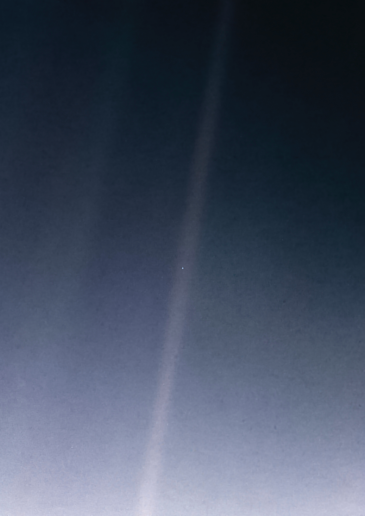
\includegraphics[width=\paperwidth,height=\paperheight,%
keepaspectratio]{images/palebluedotA4s.png}%
\vfill
}}}

%\usepackage[6-73,105-107]{pagesel}
\usepackage{tikz}
\usetikzlibrary{tikzmark}
\usetikzlibrary{arrows.meta}
% \usetikzlibrary{positioning}
% \newcommand{\tikzmark}[1]{\tikz[overlay,remember picture] \node (#1) {};}

\begin{document}
\AddToShipoutPicture*{\BackgroundPic}
\captiondelim{\quad}\captionnamefont{\footnotesize}\captiontitlefont{\footnotesize}
\selectlanguage{british}\frenchspacing

\begin{titlingpage}
\calccentering{\unitlength}
\begin{adjustwidth}{\unitlength}{-\unitlength}
  \centering
  % c6ddff % color of Earth in the Pale Blue Dot picture
  \color[HTML]{C6DDFF}
  \maketitle
\end{adjustwidth}
\end{titlingpage}
\killtitle

\calccentering{\unitlength}
\begin{adjustwidth*}{\unitlength}{-\unitlength}\thispagestyle{empty}
  \centering
  
\includegraphics[align=c,height=1em]{images/cc_by_sa.png} Licence

  \smallskip

  %%% ***%%% Luca\enspace\href{https://orcid.org/0000-0002-6070-0784}{\raisebox{0.5ex}{\protect
\includegraphics[height=1ex]{pglpm_latex/orcid_32x32.png}}}{\footnotesize\url{https://orcid.org/0000-0002-6070-0784}}

\smallskip

Typeset with \LaTeX%\ using 12\,pt Palatino and Optima fonts

\bigskip

Cover image: the \enquote{Pale Blue Dot} image of the Earth taken by Voyager~1,
\\from right outside Pluto's orbit\\
\url{https://science.nasa.gov/resource/voyager-1s-pale-blue-dot/}
\end{adjustwidth*}
\setcounter{page}{2}


%%%%%%%%%%%%%%%%%%%%%%%%%%%%%%%%%%%%%%%%%%%%%%%%%%%%%%%%%%%%%%%%%%%%%%%%%%%%
%%% Abstract
%%%%%%%%%%%%%%%%%%%%%%%%%%%%%%%%%%%%%%%%%%%%%%%%%%%%%%%%%%%%%%%%%%%%%%%%%%%%
% \abstractrunin
% \abslabeldelim{}
% \renewcommand*{\abstractname}{}
% \setlength{\absleftindent}{0pt}
% \setlength{\absrightindent}{0pt}
% \setlength{\abstitleskip}{-\absparindent}
% \begin{abstract}\labelsep 0pt%
%   \noindent Lecture notes on introductory mechanics and thermodynamics (ING175)
% % \\\noindent\emph{\footnotesize Note: Dear Reader
% %     \amp\ Peer, this manuscript is being peer-reviewed by you. Thank you.}
% % \par%\\[\jot]
% % \noindent
% % {\footnotesize PACS: ***}\qquad%
% % {\footnotesize MSC: ***}%
% %\qquad{\footnotesize Keywords: ***}
% \end{abstract}
\selectlanguage{british}\frenchspacing

%%%%%%%%%%%%%%%%%%%%%%%%%%%%%%%%%%%%%%%%%%%%%%%%%%%%%%%%%%%%%%%%%%%%%%%%%%%%
%%% Epigraph
%%%%%%%%%%%%%%%%%%%%%%%%%%%%%%%%%%%%%%%%%%%%%%%%%%%%%%%%%%%%%%%%%%%%%%%%%%%%
% \asudedication{\small ***}
% \vspace{\bigskipamount}
\setlength{\epigraphwidth}{0.66\linewidth}
% \epigraphtextposition{flushright}
% %\epigraphsourceposition{flushright}
\epigraphfontsize{\footnotesize}
\setlength{\epigraphrule}{0pt}
% % \epigraphposition{flushright}
% %\setlength{\beforeepigraphskip}{0pt}
%\setlength{\afterepigraphskip}{2em}



%%%%%%%%%%%%%%%%%%%%%%%%%%%%%%%%%%%%%%%%%%%%%%%%%%%%%%%%%%%%%%%%%%%%%%%%%%%%
%%% BEGINNING OF MAIN TEXT
%%%%%%%%%%%%%%%%%%%%%%%%%%%%%%%%%%%%%%%%%%%%%%%%%%%%%%%%%%%%%%%%%%%%%%%%%%%%

\clearpage
\phantomsection\pdfbookmark{\contentsname}{toc}
\tableofcontents*
\label{sec:toc}

\setcounter{chapter}{-1}


%%%%%%%%%%%%%%%%%%%%%%%%%%%%%%%%%%%%%%%%%%%%%%%%%%%%%%%%%%%%%%%%%%%%%%%%%%%%
%%% Preface
%%%%%%%%%%%%%%%%%%%%%%%%%%%%%%%%%%%%%%%%%%%%%%%%%%%%%%%%%%%%%%%%%%%%%%%%%%%%
\printpagenotes*
\clearpage
\addchap{Preface}
\label{cha:preface}

These notes are aimed at undergraduate students in Physics and in Engineering programmes, but graduate students may also find them useful.

You are probably aware of the variety of physics branches, such as mechanics, thermodynamics, chemistry, electromagnetics, fluid mechanics, statics, nuclear physics, and many others. Maybe you are acquainted with some of them. Probably you are also aware of the existence of different physical theories, like Newtonian Mechanics, General Relativity, Quantum Theory, which give different explanations and formulae for the same physical phenomena. Some physical theories are said to be more exact or more approximate than others; Newtonian mechanics, for instance, is an approximation of General Relativity. Does this wild variety of branches and theories also mean a wild variety of principles, methods, mathematical formulae -- which you'll have to learn if you want or need to study any particular branch or theory?

Yes, it does. But there is also a core of very few principles and one method that apply \emph{universally} to every branch and every theory known today, be it mechanics or thermodynamics, Newtonian Mechanics or General Relativity. If you learn these principles and this method, you'll be able to \emph{immediately} work with, and understand, at least the general features of \emph{every} new physical discipline, phenomenon, or technology that you might meet.

\medskip

The main goal of these notes is to make you acquainted with this core of few physical principles and this method.

How few are these principles? Around \emph{seven} (the exact number depends on how we arbitrarily group or separate them). This is the reason for the title of these notes. These seven principles are quite amazing for various reasons:
\begin{itemize}
\item They apply to \emph{every} physical phenomenon, as already mentioned.
\item Their meaning is very intuitive: each of them expresses a sort of budget.
\item They are responsible for, so to speak, \enquote{driving the universe forward in time}. More precisely, they are the basic principles that allow us to make predictions about physical phenomena.
\item Their mathematical formulation is \emph{exactly the same} in all our main approximate and exact theories, like Newtonian mechanics and General Relativity. This means that if you learn how to apply them to a tennis ball, then you are also able to apply them to a black hole.
\end{itemize}

\medskip

These universal principles are obviously expressed mathematically. Their consequences and applications can be studied, to some degree, by using analytical methods; that is, by methods involving mathematical operations that we can do by hand. But their most fascinating and practical applications need numerical methods, that is, methods involving some programming and computer simulation.

In my opinion, if you learn how to apply these universal principles in simple simulations, then you also better understand their meaning and the way they work. For this reason these notes mainly take a computational approach. We shall learn how to implement these universal principles in simple computer code, and see the fun variety of physical phenomena they lead to. Programs that accompany these notes can be found at
\begin{center}
  \url{https://pglpm.github.io/7wonders/}
\end{center}

\iftrue
\addsec{Thanks}
\label{sec:thanks}

I am deeply indebted to the students attending the ING\,175 course, Spring-term 2024, at the Western Norway University of Applied Sciences (HVL) in Bergen. They allowed me to experiment presenting physics as done in these notes, and gave invaluable feedback about what's easy and what's difficult, what's clear and what's unclear, with many suggestions for improvement, and also moral support with their curiosity and enthusiasm. In particular, in alphabetic order: %
Amalie Solberg Magnussen Rege, %
% Azzat Ammar Kouzi, %
Bodil Markhus, %
% Cristopher Gerald Rojas, %
Dag Åsmund Ørnes, %
% Erlend Vitsø, %
Iver Thoresen Malme, %
% Jonas Pytte, %
Josefine Björk Jarlesdottir Gjerde, %
Leonard Rogardt Heldal, %
Nicolai Lindløkken, %
Nikolai Ringereide, %
Oda Skagsoset Kristiansen, %
Rebecca Sahlem, %
Rudi Nathaniel Stødle, %
Severin Johannessen, %
% Sondre Moa Risnes, %
% Stein Olav Løset Frey, %
Vegard Aa Albretsen, %
William Sæther. %
Mats Øinas deserves a special thank for his thorough feedback, questions, suggestions, and encouragement.

A heartfelt thank goes to Yu-Chung Wang for his assistance in teaching and his feedback and continuous moral support.
\fi

% \addsec{Guide to the text}
% \label{sec:guide}
%
% \addsubsec{Physics prerequisites}
% \label{sec:guide_physics}
%
% Just some vague reminiscences of secondary/high-school physics should be enough.
%
% It can be beneficial if you are familiar with basic physics notions like \emph{velocity}, \emph{mass}, \emph{force}, and similar ones.
%
% \addsubsec{Maths prerequisites}
% \label{sec:guide_maths}
%
% \begin{itemize}
% \item Working familiarity with algebra, its operations and their properties.
% \item Working familiarity with solving equations and inequalities, linear and non-linear.
% \item Working familiarity with the study of functions of one real variable.
% \item Working familiarity with derivatives.
% \item Understanding of what an integral is, even if you won't be required to solve integrals.
% \item Working familiarity with vector calculus.
% \item Some familiarity with functions of many variables.
% \item Understanding of what partial derivatives are.
% \end{itemize}
%
%
% \addsubsec{Programming prerequisites}
% \label{sec:guide_program}
%
% \begin{itemize}
% \item Knowing what a computer program is.
% \item Working familiarity with variables in a computer program.
% \item Working familiarity with \texttt{for}- and \texttt{while}-loops.
% \item Working familiarity with outputting and plotting the results of a computer program.
% \end{itemize}
%
%
% \addsubsec{Structure of this text}
% \label{sec:guide_text}
%
% \subsubsection{\faIcon{hand-point-right}\enspace Graphical devices}
%
% The text includes the following graphical devices:
% \begin{itemize}[para]
% \item Important notions and definitions are also given in \textbf{boldface}.
%
% \item\label{sec:self-reference}
%   % \subsection*{\faIcon{hand-point-right}\enspace References to previous topics}
%
% The side margins often report clickable references to \autoref{sec:self-reference}{previous topics, emphasized in blue}.
%
% \item Important-notion boxes:
%   \begin{definition}{Some important notion or definition}
%     This is a definition or explanation of Something.
%   \end{definition}
% \item Warnings and important points that require careful thinking:
%   % \colorlet{shadecolor}{red}
%   % \begin{shaded}
%   %   Something you must be careful about.
%   % \end{shaded}
%   \begin{warning}[Careful!]
%     Something you must be careful about.
%   \end{warning}
% \item Exercises:
%   \begin{exercise}
%     This isn't really an exercise
%   \end{exercise}
% % \item Possible objections you might be thinking about:
% %   \begin{critique}[This isn't right!]
% %     I have an objection here.
% %   \end{critique}
% \item Discussions and connections with more advanced physics:
%   \begin{extra}{How things really are in quantum physics}
%     Just for your curiosity.
%   \end{extra}
% \end{itemize}
%
% \subsubsection{\faIcon{hand-point-right}\enspace Side pictures and quotes}
%
% \marginpar{\centering%
% 
\includegraphics[align=c,width=0.5\linewidth]{images/saitama_image.png}%
% \\[\jot]\footnotesize\flushleftright{\color{green}%
% This is an image of Saitama, which actually has nothing to do with the text on the left.}
% }%
% Pictures, graphs, or quotes related to the material are displayed on the right.
%
%
% \subsubsection{\faIcon{hand-point-right}\enspace Hyperlinks and bibliography}
%
% Some words are hyperlinks, like this one about \furl{https://onepunchman.fandom.com}{One Punch Man}; you also recognize them because they have a little footnote number. The links' URLs are listed at the end of each chapter, just in case you're reading a printed copy and wonder what the link was.
%
% \medskip
%
% The text gives bibliographic references, like \enquote{\cites{einstein1905c}}, to scientific literature. The references are listed in the final Bibliography on page~\pageref{sec:biblio}.
%
% These references are given for two reasons:
% \begin{itemize}
% \item For your own curiosity.
%
% \item
% \marginpar{\vspace{-3\baselineskip}\raggedright\footnotesize\color{mpcolor}\emph{%
% \enquote{Believe nothing, O monks, merely because you have been told it, or because it is traditional, or because you yourselves have imagined it. Do not believe what your teacher tells you merely out of respect for the teacher.}}
% \\[\jot](attributed to Gautama Buddha)
% }%
% To back up what's written in the text.
% In science you should not believe something just because you've read it somewhere. You should, as much as possible, \emph{go and check for yourself how the logic behind the statement is proved and what is the experimental evidence behind the statement}.
% \end{itemize}
%
% \subsubsection{\faIcon{hand-point-right}\enspace Notation and terminology}
%
% Mathematical notation, as well as notation for physical dimensions, strictly follows the standards given by the \furl{https://www.nist.gov/pml/special-publication-811}{International System of Units (SI)}, listed for example in \cites{iso2009} and \cites{iso2019}.











\clearpage
\addchap{Guide to the text}
\label{cha:guide}

\addsec{Physics prerequisites}
\label{sec:guide_physics}

Just some vague reminiscences of secondary/high-school physics should be enough.

It can be beneficial if you are familiar with basic physics notions like \emph{velocity}, \emph{mass}, \emph{force}, and similar ones.

\addsec{Maths prerequisites}
\label{sec:guide_maths}

\begin{itemize}
\item Working familiarity with algebra, its operations and their properties.
\item Working familiarity with solving equations and inequalities, linear and non-linear.
\item Working familiarity with the study of functions of one real variable.
\item Working familiarity with derivatives.
\item Understanding of what an integral is, even if you won't be required to solve integrals.
\item Working familiarity with vector calculus.
\item Some familiarity with functions of many variables.
\item Understanding of what partial derivatives are.
\end{itemize}


\addsec{Programming prerequisites}
\label{sec:guide_program}

\begin{itemize}
\item Knowing what a computer program is.
\item Working familiarity with variables in a computer program.
\item Working familiarity with \texttt{for}- and \texttt{while}-loops.
\item Working familiarity with outputting and plotting the results of a computer program.
\end{itemize}


\addsec{Structure of this text}
\label{sec:guide_text}

\subsubsection{\faIcon{hand-point-right}\enspace Graphical devices}

The text includes the following graphical devices:
\begin{itemize}[para]
\item Important notions and definitions are also given in \textbf{boldface}.

\item\label{sec:self-reference}
  % \subsubsection{\faIcon{hand-point-right}\enspace References to previous topics}

The side margins often report clickable references to \autoref{sec:self-reference}{previous topics, emphasized in blue}.

\item Important-notion boxes:
  \begin{definition}{Some important notion or definition}
    This is a definition or explanation of Something.
  \end{definition}
\item Warnings and important points that require careful thinking:
  % \colorlet{shadecolor}{red}
  % \begin{shaded}
  %   Something you must be careful about.
  % \end{shaded}
  \begin{warning}[Careful!]
    Something you must be careful about.
  \end{warning}
\item Exercises:
  \begin{exercise}
    This isn't really an exercise
  \end{exercise}
% \item Possible objections you might be thinking about:
%   \begin{critique}[This isn't right!]
%     I have an objection here.
%   \end{critique}
\item Discussions and connections with more advanced physics:
  \begin{extra}{How things really are in quantum physics}
    Just for your curiosity.
  \end{extra}
\end{itemize}

\subsubsection{\faIcon{hand-point-right}\enspace Side pictures and quotes}

\marginpar{\vspace{-4\baselineskip}\centering%

\includegraphics[width=0.5\linewidth]{images/saitama_image.png}%
\\[\jot]\footnotesize\flushleftright{\color{green}%
This is an image of Saitama, which actually has nothing to do with the text on the left.}
}%
Pictures, graphs, or quotes related to the material are displayed on the right.


\subsubsection{\faIcon{hand-point-right}\enspace Cross-references}

The text gives cross-references to the main section where a topic was discussed or will be discussed. Cross-references appear as section number and page listed on the margin, like this cross-reference to \autoref{sec:conservation_laws}{conservation laws}.


\subsubsection{\faIcon{hand-point-right}\enspace Hyperlinks and bibliography}

Some pieces of text are hyperlinks, like this one about \furl{https://onepunchman.fandom.com}{One Punch Man}. You recognize them from their different colour and from the little footnote number that follows them. The links' URLs are also listed at the end of each chapter, in case you're reading a printed copy of these notes.

\medskip

The text gives bibliographic references, like \enquote{\cites{einstein1905c}}, to scientific literature. The references are listed in the final Bibliography on page~\pageref{sec:biblio}.

These references are given for two reasons:
\begin{itemize}
\item For your own curiosity.

\item
\marginpar{\vspace{-1\baselineskip}\raggedright\footnotesize\color{mpcolor}\emph{%
\enquote{Believe nothing, O monks, merely because you have been told it, or because it is traditional, or because you yourselves have imagined it. Do not believe what your teacher tells you merely out of respect for the teacher.}}
\\[\jot](attributed to Gautama Buddha)
}%
To back up what's written in the text.
In science you should not believe something just because you've read it somewhere. You should, as much as possible, \emph{go and check for yourself how the logic behind the statement is proved and what is the experimental evidence behind the statement}.
\end{itemize}

\subsubsection{\faIcon{hand-point-right}\enspace Notation and terminology}

Mathematical notation, as well as notation for physical dimensions, strictly follows the standards given by the \furl{https://www.nist.gov/pml/special-publication-811}{International System of Units (SI)}, listed for example in \cites{iso2009} and \cites{iso2019}.


\printpagenotes*
\clearpage
\chapter{Overview}
\label{cha:overview}

\addsec{The plan of these notes}

After some very general remarks about physics, we recall the notions of \textbf{physical quantity}, unit, and physical dimension. This is really just a reminder; it's assumed that you are already familiar with these general notions.

We then survey two cardinal physical notions: \textbf{time} and \textbf{space}. We briefly examine their fascinating nature as we today understand it. The notion of \textbf{coordinate system} is also introduced.

Thereafter we take an overview of the main seven physical quantities we shall work with: \textbf{matter}, \textbf{energy-mass}, \textbf{momentum}, \textbf{angular momentum}, \textbf{entropy},  \textbf{electric charge}, \textbf{magnetic flux}, discussing some features common to all of them. Other important quantities such as \textbf{temperature} are also introduced.

The most important feature of the main seven quantities is that we can measure their amount within any volume, and the amount that passes through any surface. We therefore study the intuitive ideas of \textbf{control volume} and \textbf{volume content}, \textbf{control surface} and \textbf{flux}, and \textbf{supply}.

At this point the stage is ready for the introduction of seven physical laws which are just expressions of \textbf{balances} of volume contents, fluxes, and supplies of the seven quantities introduced earlier. These seven balance laws are universal. They are connected by mathematical expressions called \textbf{constitutive relations}, which are not universal but depend on the particular physical phenomenon, and on the particular physical theory we use to describe it.

The balance laws are the ones that allow us to predict how the values of different quantities change with time. We show this by exploiting them to build simple computer code that can in principle be applied to any physical system. The role that constitutive relations have in connecting the seven balances also becomes quite clear in the code.

Five of the seven universal balances are then examined in turn. For each balance, we study some constitutive relations that are often used together with it, as well as some of its physical applications.

\addsec{Physics?}
\label{sec:physics_general}

% \section{Magic}
% \label{sec:magic}

If you think about it, many things we ordinarily do every day are some sort of magic. Think of how you can instantaneously see and speak with a person living on another continent, in real time, using just a small widget in the palm of your hand. Think of how you can instantaneously see where you are on the Earth, using the same widget. Think of how fast you can go to another country, by flying in a huge metal thing. Think of how you can command and interact with a purely fictitious animated world when you play on your computer. The list can go on forever. Other things are luckily less ordinary, but still inspire a lot of awe: think of the devastating power unleashed by something roughly as small as a tennis ball, in an atomic bomb.

We can do these astonishing things thanks to our understanding of how the world works. That's Physics.

\medskip

Many things can be said and have been said about science and physics. Rather than repeating what's been already written in many excellent books, I invite you to take a break here and go read their introductions. Choose as you please; compare what they say; don't limit yourself to popular books.

% \begin{center}
%   \textellipsis
%   \textellipsis
%   \textellipsis
% \end{center}



\addsec{What is \enquote{fundamental} physics?}
\label{sec:fundamental_physics}

But what's the \enquote{ultimate} goal of physics? What's \enquote{fundamental} physics? The answer to this question is again subjective -- also in this case physics lets you express your proclivities and personality. In the history of physics one can probably identify two main conceptions of \enquote{fundamental} physics.

For some physicists it is about finding the ultimate building blocks, so that one day we can say \enquote{\textellipsis and these are the constituents, and they obey these equations}. The history of physics seems to show that this goal is overturned every few generations. And yet every generation says \enquote{\emph{Now} we almost have the complete picture -- it's right behind the corner. It's true that previous generations thought they almost had it, and turned out to be wrong. But \emph{this time} is different, this time we have the real deal!}. The theoretical and particle physicist \furl{https://www.physics.lbl.gov/rememberinggeoffreychew/}{Geffrey Chew} depicted this situation as in \fig\,\ref{fig:chew1}. For this reason some physicists are a little sceptical about this goal; maybe it's a never-ending structure, with surprises at every deeper look.

So for other physicists fundamental physics is about finding some point of view or mathematical structure that is rich enough to make useful predictions, and yet flexible enough to accommodate any new patterns or objects that we might discover. In a manner of speaking, it is about finding \enquote{patterns of patterns} or \enquote{laws about physical laws}.

The two conceptions above are not mutually exclusive, and both are always pursued, even if time-changing fashions may emphasize the one or the other.

In these notes we take a point of view slightly closer to the second conception. This will also be reflected in the main division between physical laws that we'll draw in \chap\,\ref{cha:laws}.


\begin{figure}[p]
  \centering
  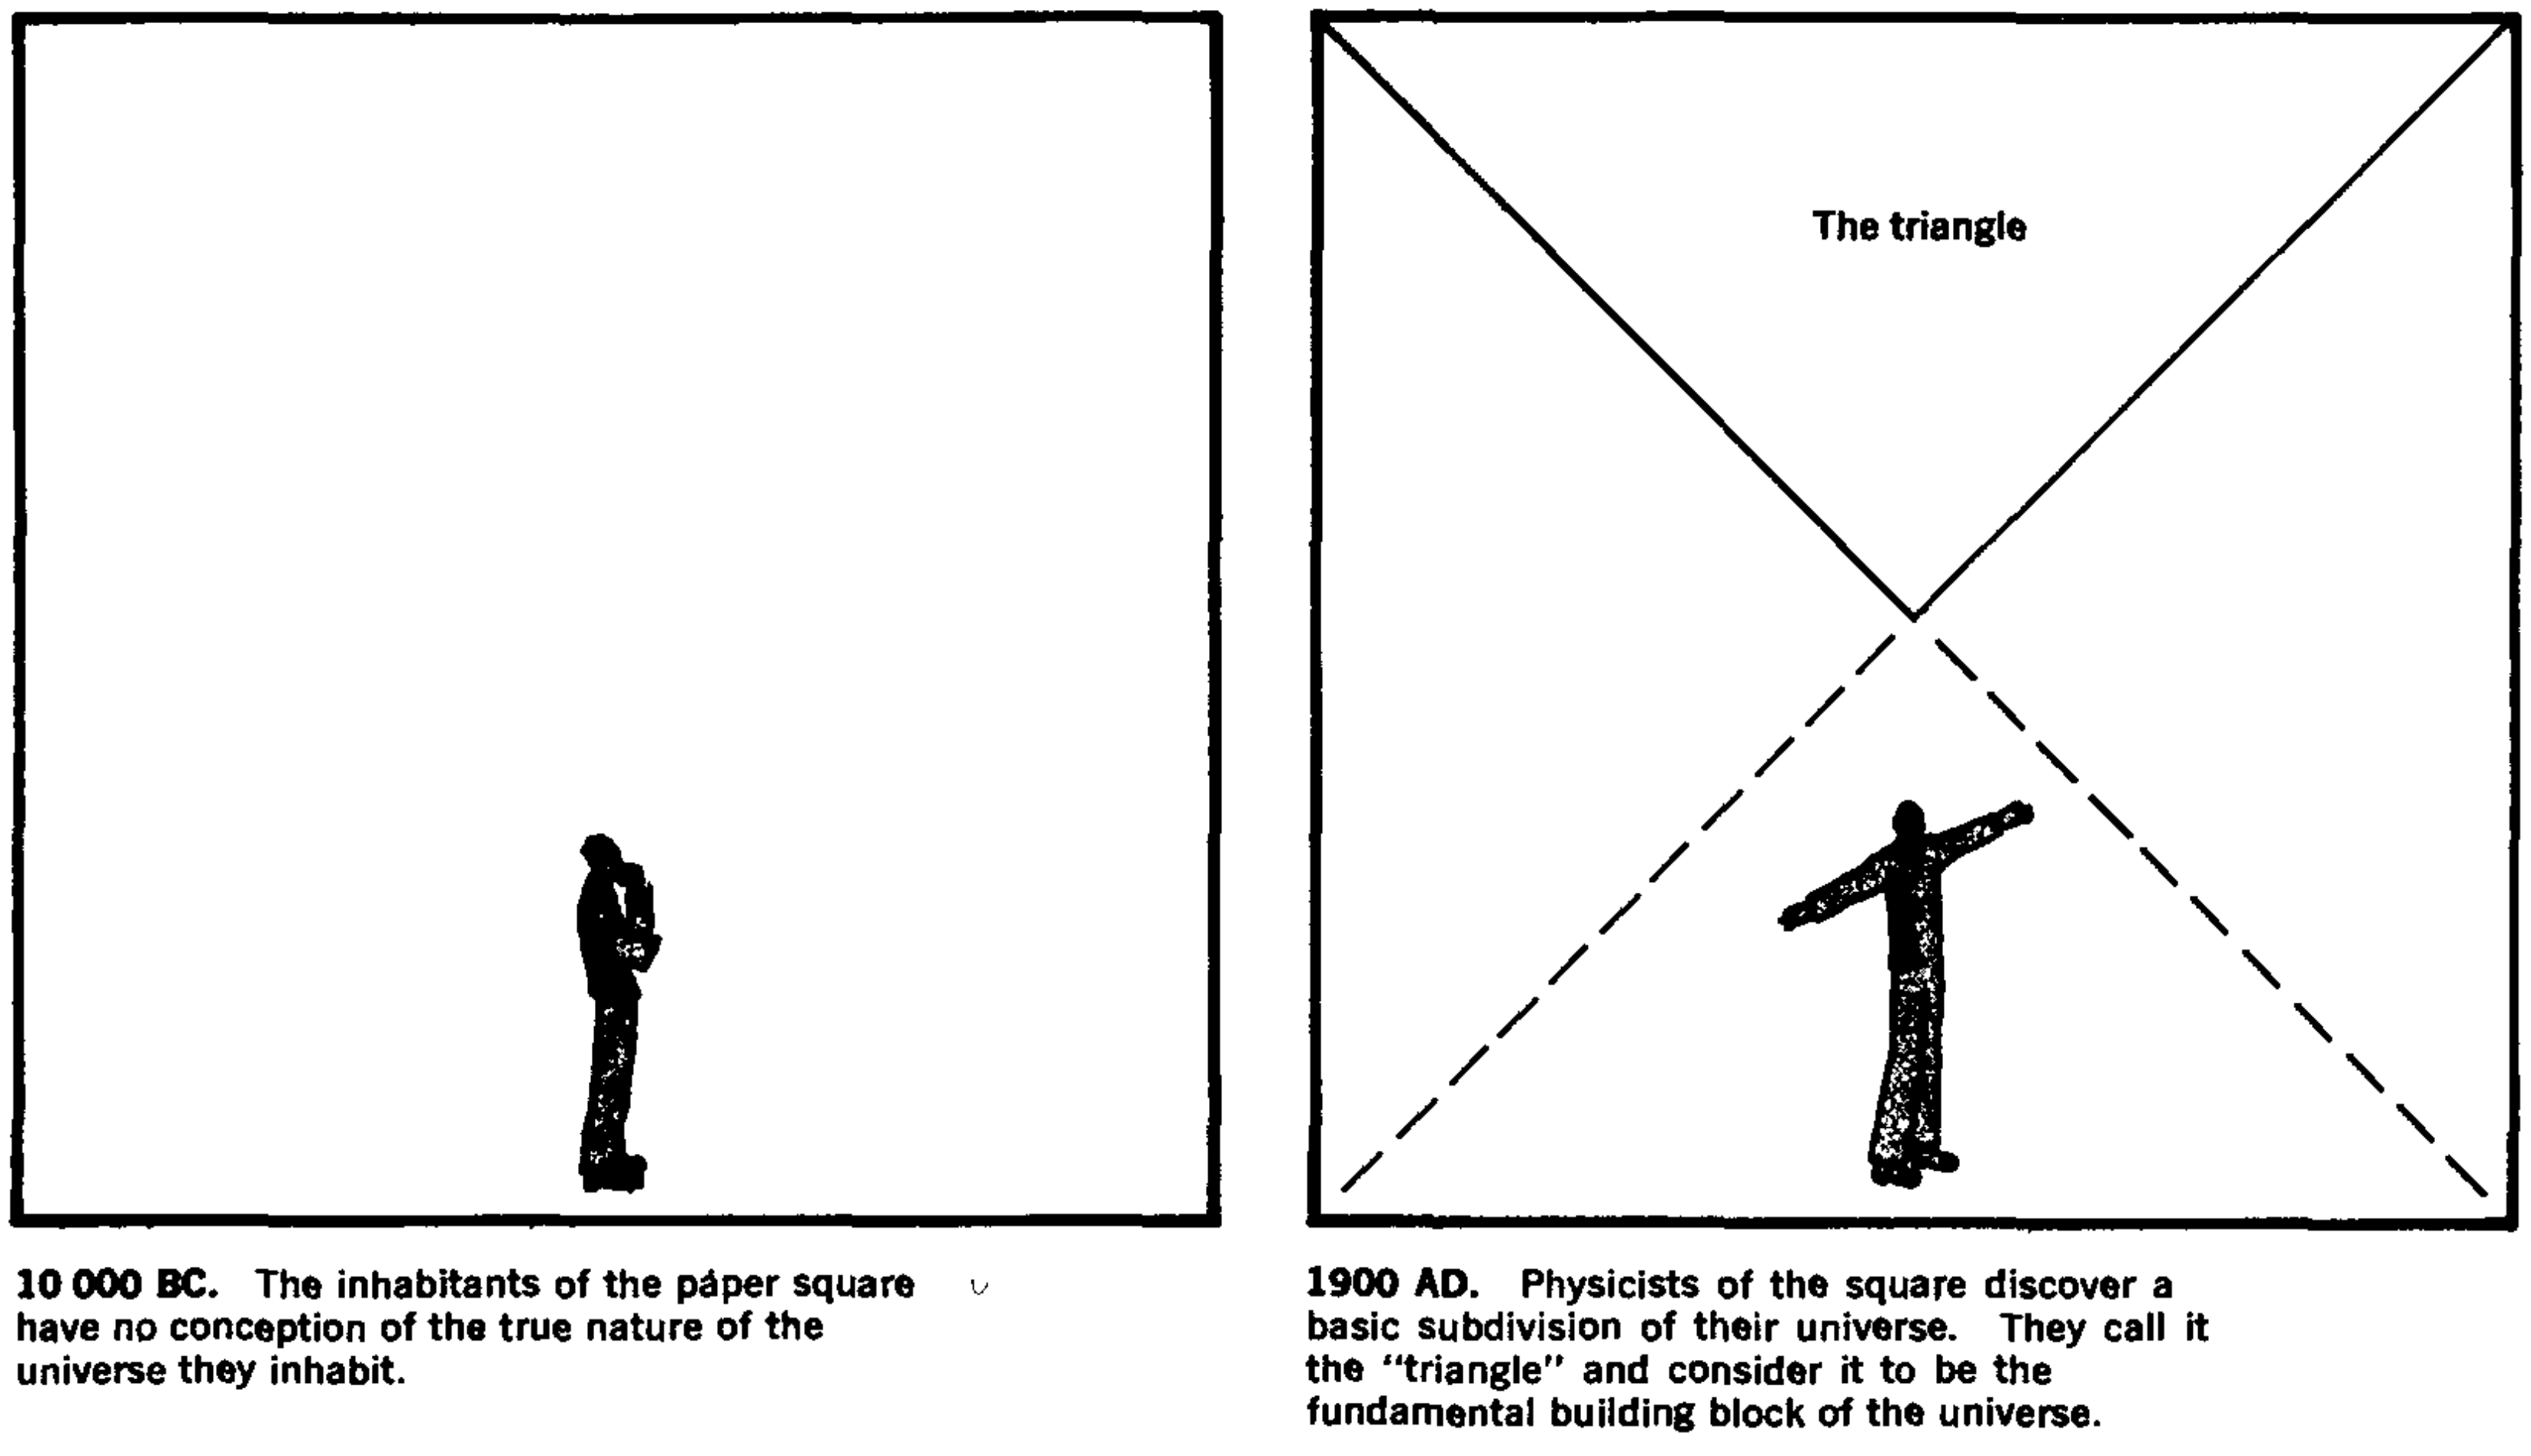
\includegraphics[width=1.2\textwidth]{images/chew1.png}
  \\[1em]  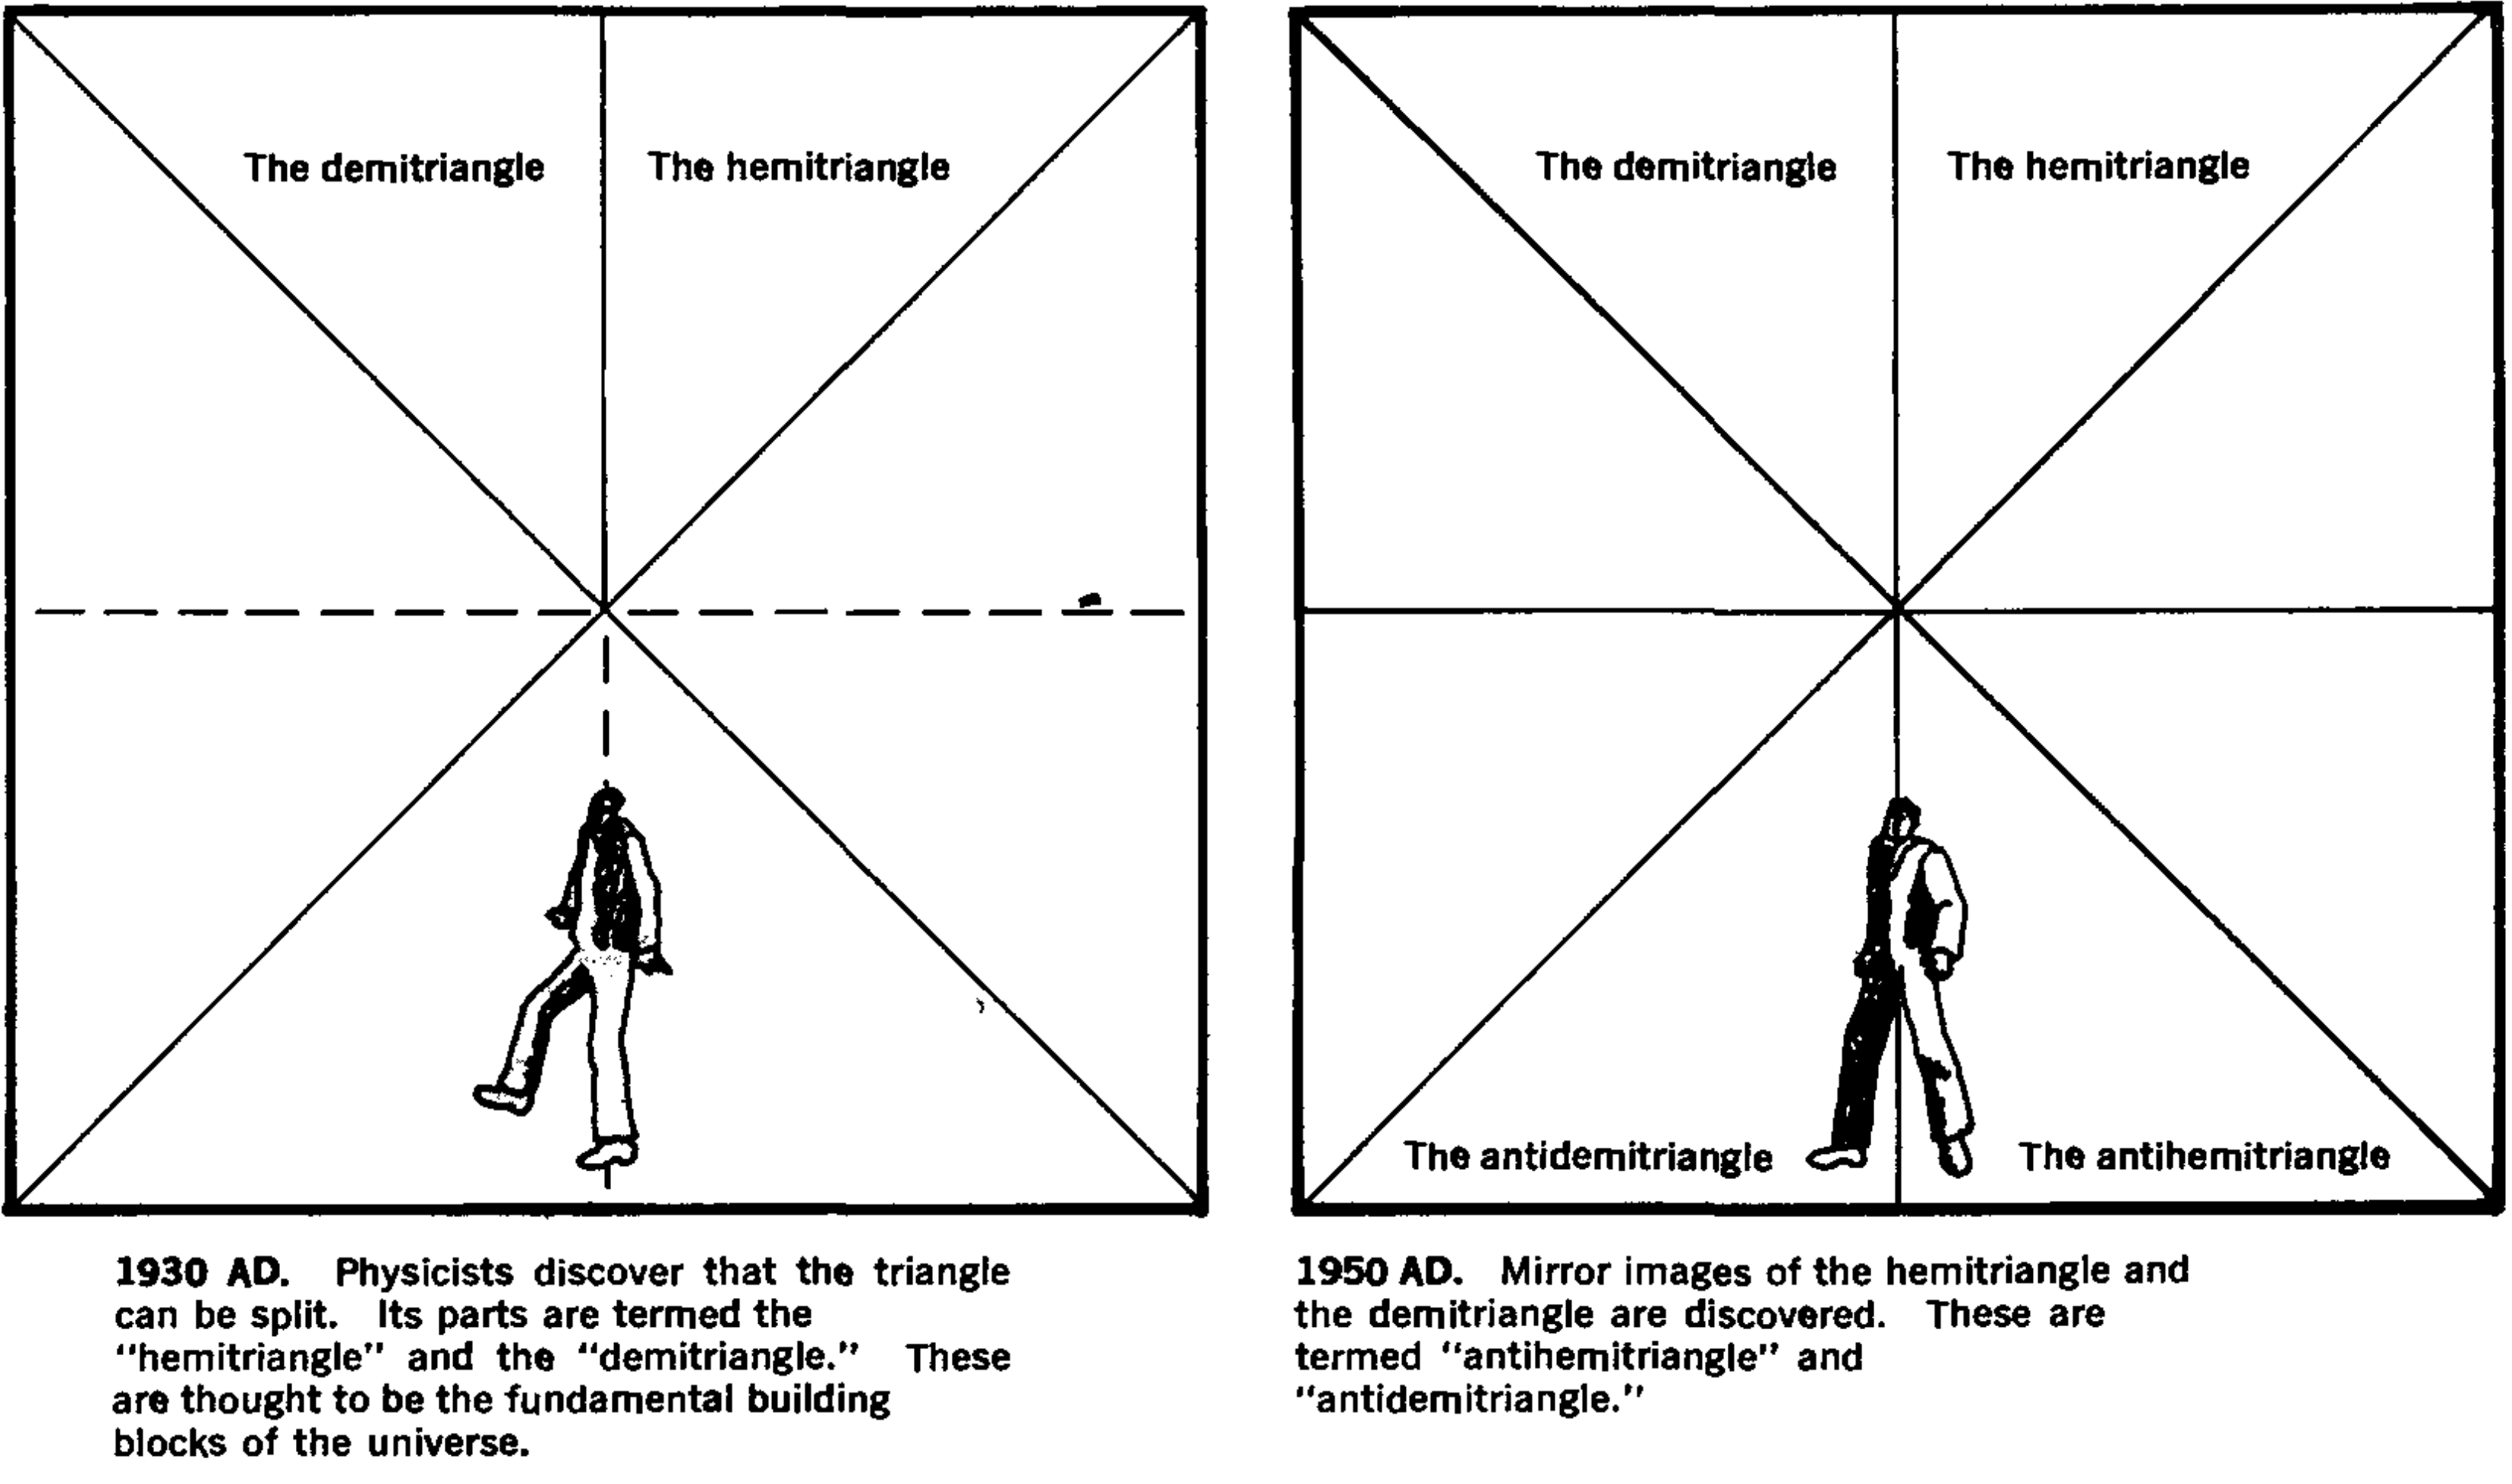
\includegraphics[width=1.2\textwidth]{images/chew2.png}
  \caption{(Continues on p.\,\pageref{fig:chew2}) \emph{The progress of \enquote{fundamental} physics}, from \cites{chew1970} as reproduced in \cites{truesdell1984_r1987}}
  \label{fig:chew1}
\end{figure}
\begin{figure}[p]
  \centering
  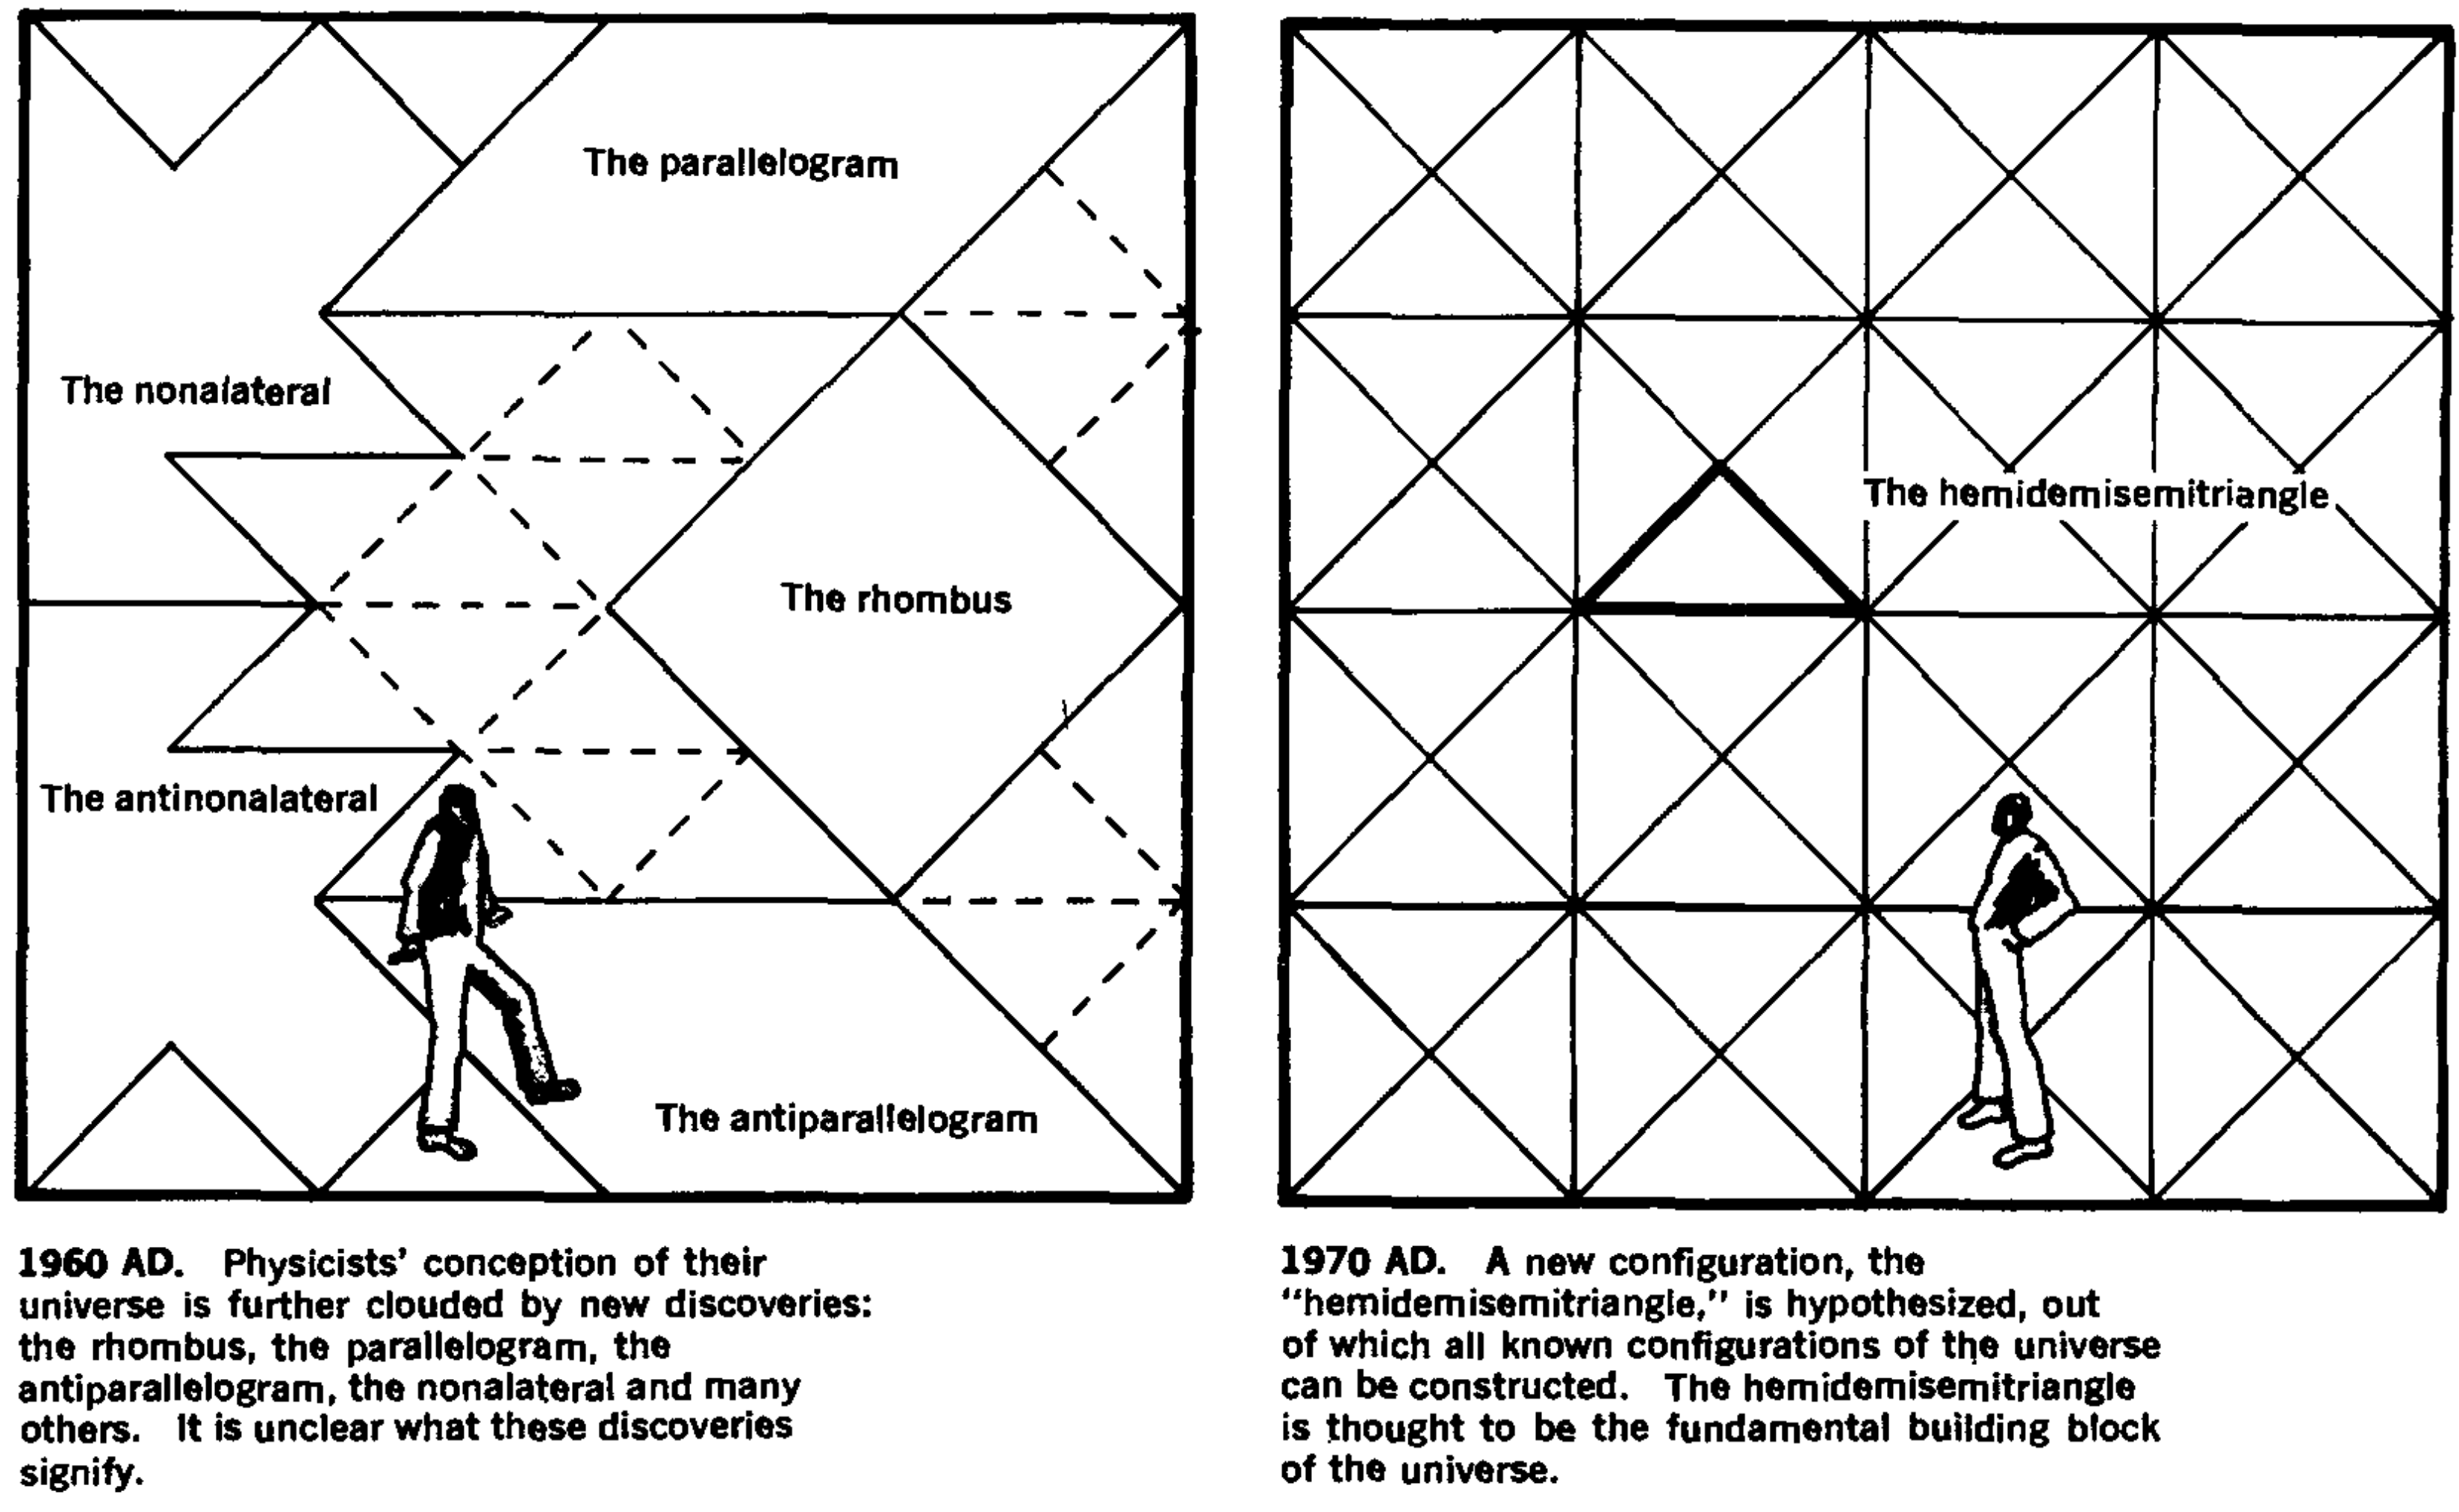
\includegraphics[width=1.2\linewidth]{images/chew3.png}
\\[1em]  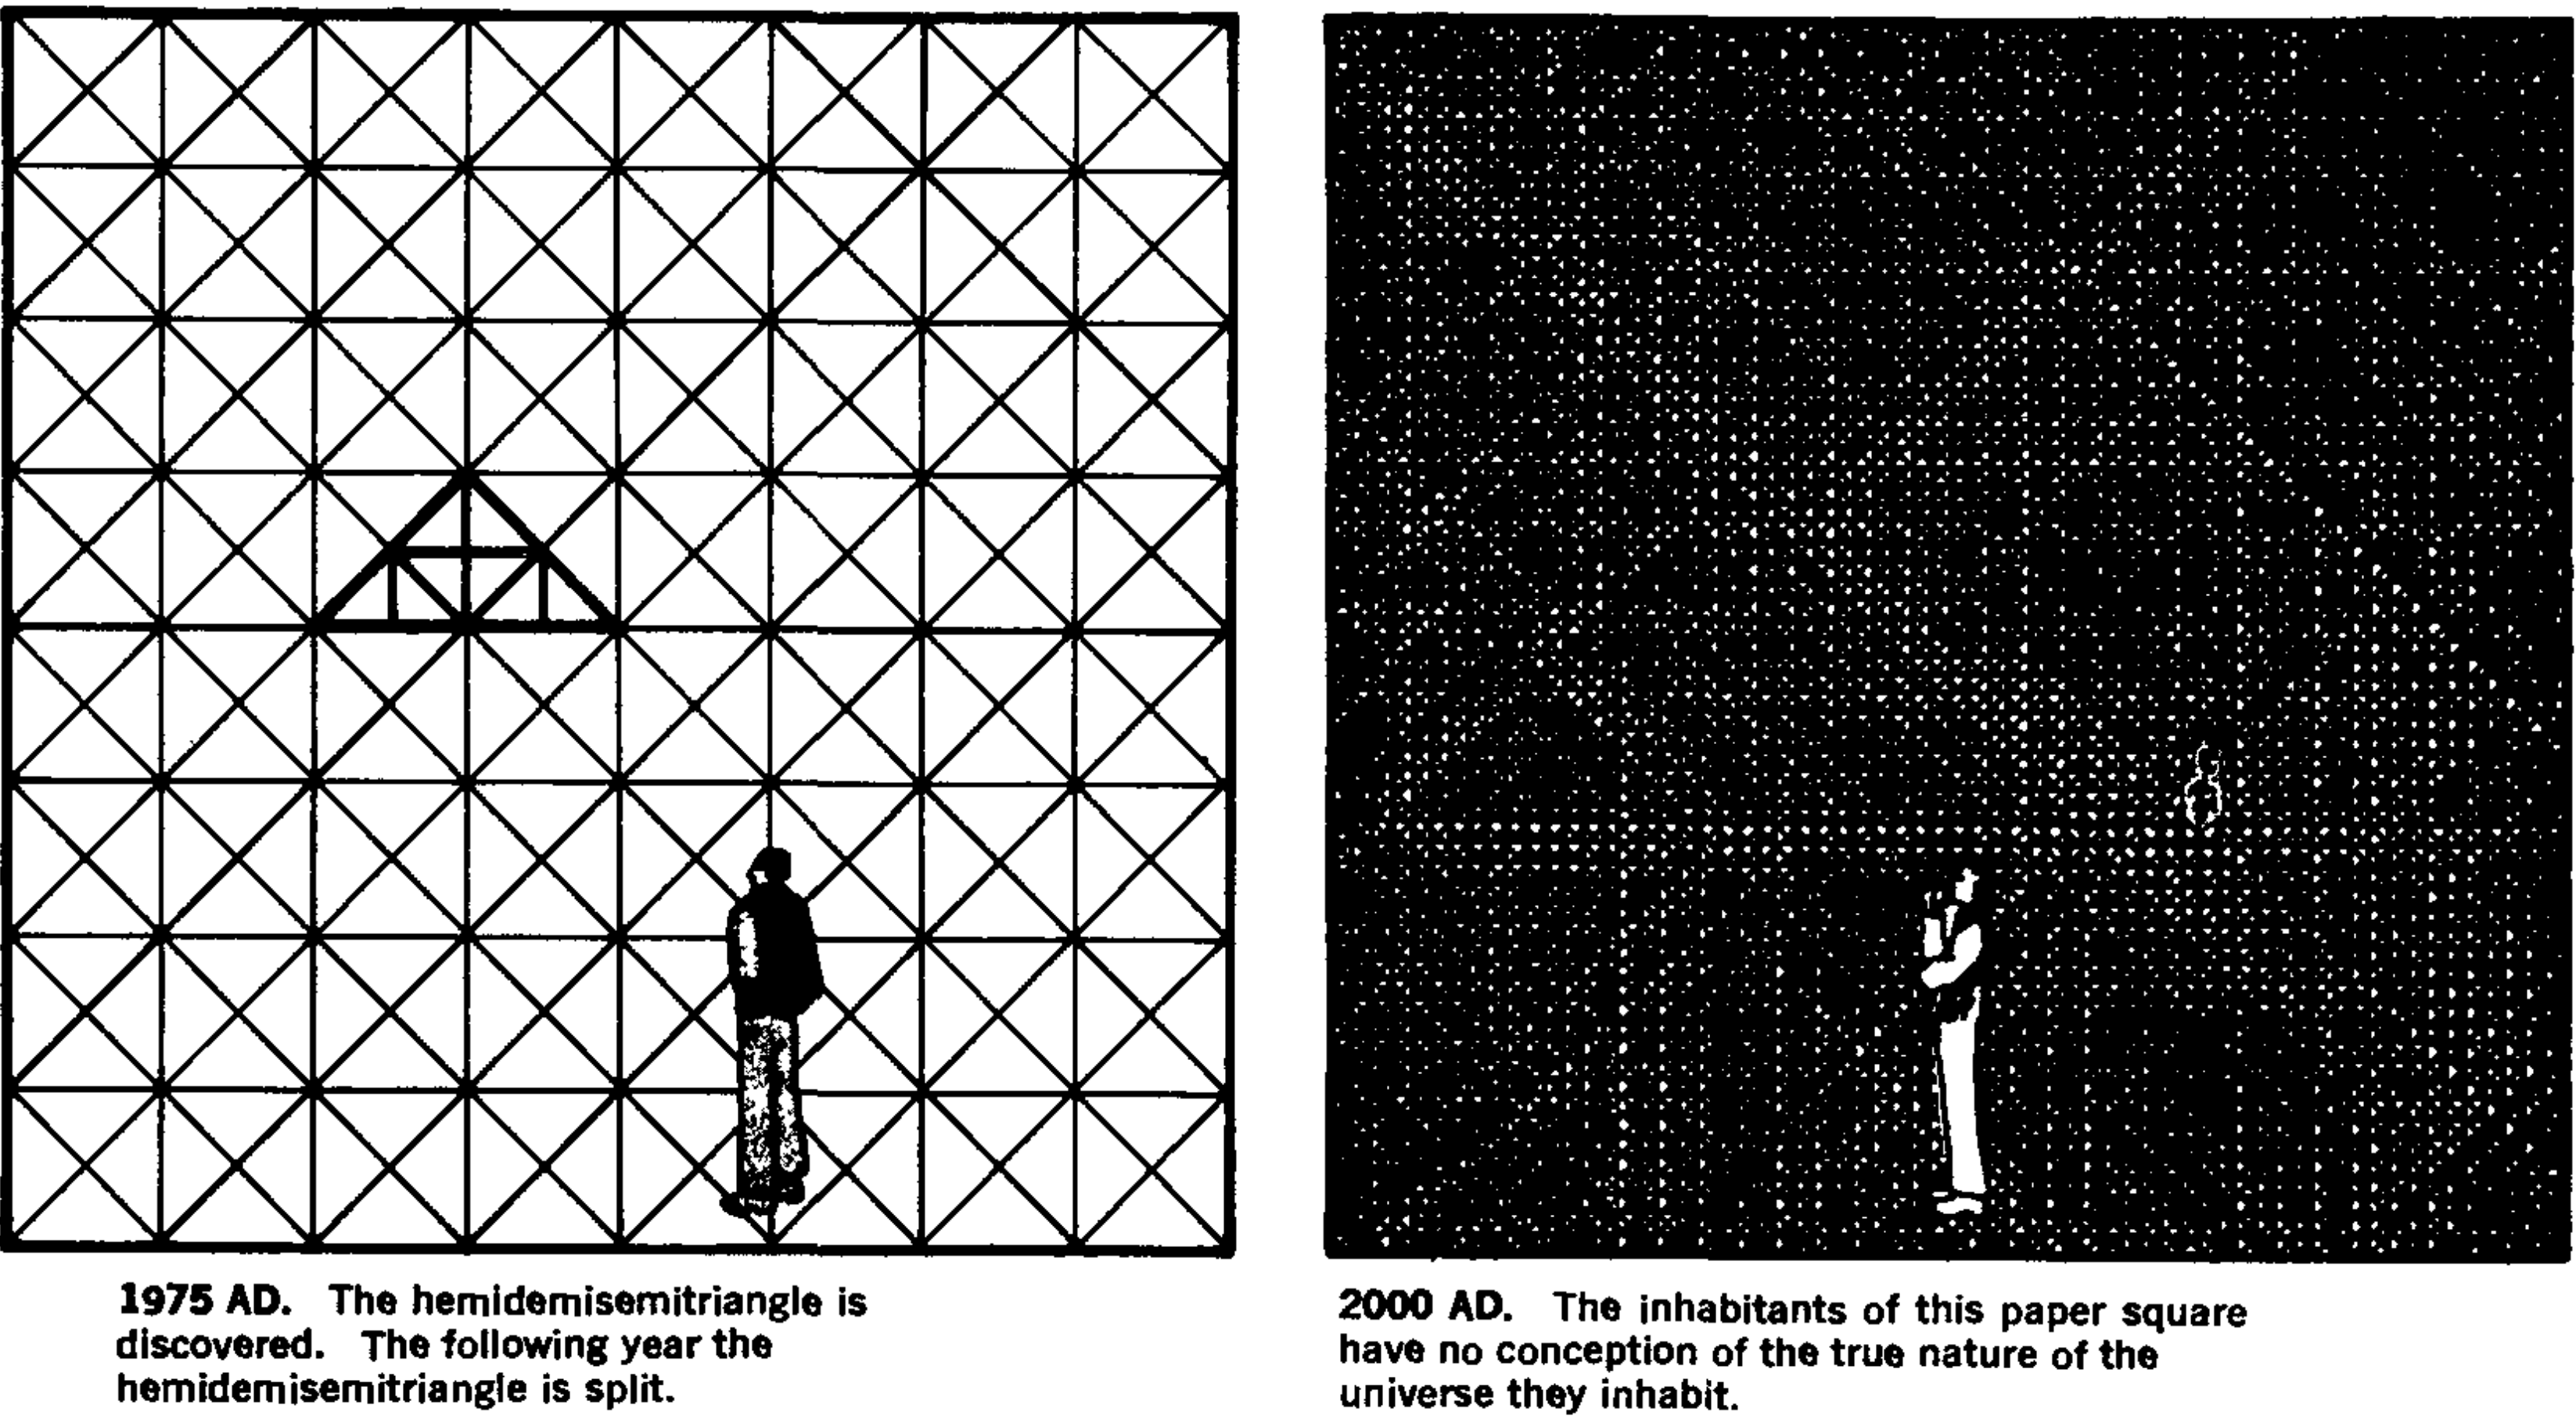
\includegraphics[width=1.2\linewidth]{images/chew4.png}
  % \caption{\emph{\enquote{The progress of \enquote*{fundamental} physics, conceived by Berkeley Chew, published in 1970 by his father, Professor Geoffrey F. Chew.}} Reproduced from  \cites{truesdell1984_r1987}}
  \label{fig:chew2}
\end{figure}


\printpagenotes*
\clearpage
\chapter{Physical quantities}
\label{cha:physical_quantities}

\epigraph{Philosophy is written in this grand book, the universe, which stands continually open to our gaze. But the book cannot be understood unless one first learns to comprehend the language and read the letters in which it is composed. It is written in the language of mathematics, and its characters are triangles, circles, and other geometric figures without which it is humanly impossible to understand a single word of it.}{G. Galilei \cites*{galilei1623}}


\section{Several possible formalisms or \enquote{languages}}
\label{sec:languages}

% Welcome back! The only thing about physics that I need to say here is that
Physics can be expressed and written from wildly different points of view, using wildly different principles. Let's call these \enquote{different physics languages}; a more technical name is \enquote{physics formalisms}. One may approach a physics phenomenon or problem in terms of \emph{Lagrangeans}, or \emph{Hamiltonians}, or \emph{fibre bundles}, or \emph{categories}, or \emph{action principles}, or many other formalisms.
\marginpar{\normalsize%
  \begin{gather*}
    \color{red}\delt\!\!\int\!\!L\,\di t = 0 \quad L=\frac12 m v^{2}
    \\
    \color{cyan}\bm{F}=\frac{\di}{\di t}m\bm{v} \quad \bm{F}=0
  \end{gather*}
%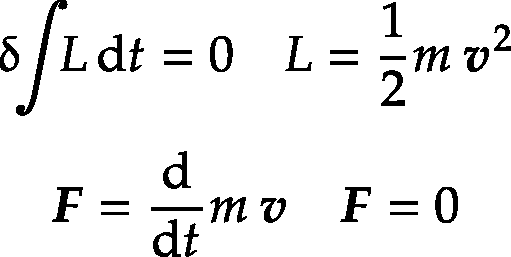
\includegraphics[align=t,width=\linewidth]{images/eg_languages.png}
\footnotesize\color{mpcolor}%
Example of two different formalisms (\textcolor{red}{red}, \textcolor{cyan}{blue}) expressing the same physical phenomenon.%
}
These formalisms or languages are not completely separated; we know how to translate among them. In \enquote{doing} physics, one may jump among formalisms, because some ideas may be easier to express, or some results easier to find, in one formalism than another. No matter which physics formalism you choose, the results and the concrete applications are still the same. The choice is to a great extent subjective, based on your aesthetic tastes. You see that in \enquote{doing} physics you can express your personality and put your own artistic touch; this is why it's such a cool subject (and other scientific subjects are like this too).

In these notes I'm choosing one particular formalism: the one that for me is the most easily \emph{visualizable}; because I believe that visualization can be beneficial in learning new things. Or maybe I'm choosing it just because I like it best. I encourage you to explore how the physics you've learned is expressed in other physics formalisms; maybe you'll like another physics formalism better.

The formalism we'll be using might be called \enquote{field theory}. Roughly speaking it takes as starting point the ideas of space and time, or better spacetime, in which there are different kinds of \enquote{stuff}. It expresses the regularity and patterns that we observe in physical phenomena as \enquote{budgets} about the different kinds of stuff, and of relations between these kinds. Please don't take the description just given too literally; it's just meant to give you a very vague idea of the field-theoretical viewpoint.

\medskip

% \marginpar{\footnotesize%
% \color{mpcolor}\enquote{\emph{this grand book, the universe, which stands continually open to our gaze. But the book cannot be understood unless one first learns to comprehend the language and read the
% letters in which it is composed. It is written in the language of
% mathematics}}\sourceatright{\cites{galilei1623}}
% }
It goes without saying that all these \enquote{physics languages} are to a great extent mathematical.

One reason is that numbers allow us to convey information in a concise and precise way. Imagine you have to tell someone, who doesn't know
Bergen, where in Bergen you are right now, to within 10\,m. You can do that with a description, \enquote{\textellipsis\ and there's a building called so-and-so which looks like so-and-so\textellipsis}, which would be lengthy and tricky. Or you can just give two numbers: latitude and longitude:
\begin{equation*}
  \num{60.36940},\ \num{5.3518} \ .
\end{equation*}
And in these two numbers all digits are important; for instance, the latitude is not \ensuremath{60.369\,4\bm{7}}.

But the most important reason is that mathematics allows us to describe and follow the patters and variety of physical phenomena in a greatly concise and precise way. And to develop their relationships in a rigorous way.
\marginpar{\footnotesize%
\color{mpcolor}\enquote{\emph{There is nothing that can be said by mathematical symbols and relations which cannot also be said by words. The converse, however, is false. Much that can be and is said by words cannot successfully be put into equations, because it is nonsense.}}\sourceatright{\cites{truesdell1966}}
}
All our present technology would have been impossible to discover, and would be impossible to realize, without the mathematical language of physics.

I invite you again to read what many good texts say about the relationship between physics and mathematics. No point repeating here what is said better elsewhere.

\section{Quantities: primitive and derived}
\label{sec:primitives}

One topic must be briefly discussed because it's important for understanding the notes that follow. It's the distinction between \emph{primitive} and \emph{derived} quantities.

I shall assume that you already know what a \textbf{physical quantity} is. Examples are: position, duration, velocity, pressure, energy, temperature.

A \textbf{derived quantity} is one that is defined in terms of other quantities. For example, velocity $\bm{v}$ (more precisely: average velocity) is defined as the ratio between a distance $\bm{d}$ (a vector) and a time duration $\bm{t}$:
\begin{equation*}
  \bm{v} \defd \frac{\bm{d}}{t}
\end{equation*}
where the symbol \enquote{$\defd$} means \enquote{is defined as} or \enquote{is defined by}. This means that in principle we could avoid using the word \enquote{velocity} and the symbol \enquote{$\bm{v}$} altogether, and instead always speak about distance and duration, using their symbols. It would lead to very long sentences and formulae and would be extremely inconvenient, but it could be done. The definition of a derived quantity often tells us how that quantity can be measured.

A derived quantity is defined in terms of other quantities, and these may in turn be derived quantities, that is, defined in terms of still other quantities, and so on. But at some point this chain of definitions must come to an end, otherwise we would go around in circles.
\marginpar{\vspace{-\baselineskip}\centering%
\href{https://www.youtube.com/watch?v=nYg6jzotiAc&t=893s}{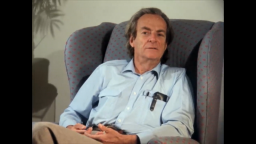
\includegraphics[width=\linewidth]{images/feynman_why2.png}}%
\\[\jot]%
\flushleftright\footnotesize\color{mpcolor}%
\emph{\enquote{you have to be in some framework that you allow something to be true. Otherwise you're perpetually asking \enquote*{why}}.}
(\furl{https://www.youtube.com/watch?v=nYg6jzotiAc&t=893s}{see video}).%
}%

A \textbf{primitive quantity} is one that we do not define in terms of other quantities. Primitive quantities are the building blocks from which we define all others. That they are not defined in terms of others doesn't mean that we cannot try to explain them. But such explanations must be taken as informal and heuristic. Primitive quantities are often explained through metaphors and by appealing to intuition. You must always be wary of such explanations, because they may fail you spectacularly in some situations.

Often we have a choice about which quantities should be primitive and which should be derived. For instance, \emph{energy} can be defined, in a somewhat complicated way, in terms of quantities like \emph{work} and \emph{heat}, which would then need to be taken as primitive. Or we can take \emph{energy} as primitive, and define \emph{work} and \emph{heat} in terms of it. This second choice can be more convenient to develop a physical theory. It often happens that a quantity is very convenient for building a theory, if used as primitive; but difficult to understand intuitively. Vice versa,  a quantity can be very intuitive but lead to a complicated theory.
Among quantities which we'll take as primitive are:
\emph{time}, \emph{space} and \emph{length}, \emph{matter}, \emph{energy}, \emph{momentum},
% , \emph{rotational momentum},
\emph{entropy}, \emph{temperature}, and several others. All will be discussed soon.

 \section{Physical dimensions and units}
\label{sec:units}

\textbf{Measurement} is the process by which we determine the value of a physical quantity. Measurements can be extremely complex, and can extremely different even if they are about the same quantity. Consider the ways we can measure the mass of a football, compared to the ways we can measure the mass of the Sun.

To each quantity we associate a \textbf{physical dimension}. The term \enquote*{dimension} here has nothing to do with physical extension, as in \enquote{the dimensions of this box}; be careful not to confuse the two. Usually it's clear which one is meant from the context. Physical dimensions help us avoid making operations that don't make sense with some quantities. For example, it doesn't make sense to sum up the volume of a body of water with its temperature; and indeed the volume has dimension $\mathsf{length^{3}}$, whereas temperature has dimension $\mathsf{temperature}$, and quantities with different dimensions cannot be added up.

With each physical dimension we can associate a measurement \textbf{unit}, which expresses a basic standard for comparing the measurement results of similar quantities. For example, we could use the \emph{minute} or the \emph{second} as units to measure $\mathsf{time}$.

One can choose a basic set of physical dimensions from which to define all others, and for these a set of standard units. Here we shall follow the
\furl{https://www.nist.gov/pml/owm/metric-si/si-units}{International System of Units (SI)} (see also \furl{https://www.nist.gov/pml/special-publication-811}{NIST Special Publication 811}).

The topics of measurement and physical dimensions, which are studied in \emph{metrology} and in \emph{dimensional analysis}, could occupy an entire course by themselves. I shall assume that you already know their basics notions and that you read about the SI.

\smallskip

The measurement of some physical quantities consists in just one number with associated physical dimension; we shall call such quantity a \textbf{scalar}. The measurement of other physical quantities consists instead in a triplet of numbers with associated physical dimension; we shall call such quantity a \textbf{vector}.
\begin{warning}[What's scalar or vector depends on the theory]
  \emph{Scalar} and \emph{vector} have very specific and slightly different meanings in different theories, so don't take the definitions used here as universal. For example, in these notes and in Newtonian mechanics we call \emph{energy density} a scalar, but in General Relativity it cannot be called a scalar.
\end{warning}

\section{Informal tips about units and maths}
\label{sec:units_maths}

\subsection{Importance of units}
\label{sec:importance_units}

Units are very important and must always be written for several reasons.

First, a number without units doesn't tell us anything. If I tell you \enquote{the place is at a distance 100 from here}, you have no idea how far the place is. \enquote{100} what? 100~metres? 100~kilometres? These are completely different distances.

Second, units give us useful information about mathematical objects and their physical relationships and measurement. If you see the expression \enquote{\qty{3}{m/s}}, then there's a strong possibility that that's a velocity. If you see the expression \enquote{\qty{5}{J/m^2}}, then you have a hint that it could be measured by measuring an energy and then dividing by an area.

Third, because of the previous reason, keeping track of units often allows us to quickly catch errors in solving a physical problem.

\subsection{Variables and units}
\label{sec:variables_units}

When a physical quantity is denoted by a symbol or variable, keep in mind that a unit is \enquote{contained} in the symbol, so to speak. For example if the variable $t$ denotes a time, then it includes some time unit, say seconds. This becomes apparent when we write the value of the symbol, for instance \enquote{$t=\qty{120}{s}$}. The unit is not predetermined, but it must correspond to the dimension of that quantity. We could for instance write \enquote{$t=\qty{2}{min}$} instead; the two expressions are completely equivalent.

This fact must be kept in mind when combining symbols. For example, if $d$ is a distance and $t$ is a time, then writing $v=d/t$ tells us that $v$ is a velocity, and it has appropriate units that come from $d$ and $t$, for instance \unit{m/s}.

Units otherwise behave just like \emph{literal constants} for all mathematical purposes, just like the letter \enquote*{$a$} in the expression \enquote*{$a\, x$}. This is why they can be simplified; for instance:
\begin{equation*}
  \qty{3}{mol/s} \cdot \qty{5}{s} =
  \num{3}\:\frac{\unit{mol}}{\mathcolor{red}{\not}\!\unit{s}} \cdot \num{5}\:\mathcolor{red}{\not}\!\unit{s} = \qty{15}{mol} \ .
\end{equation*}

\subsection{Mathematical functions and units}
\label{sec:functions_units}

Particular care must be taken with trigonometric and exponential functions, like $\sin()$, $\cos()$, $\tan()$, $\exp()$, $\log()$; \textbf{these functions only admit a dimensionless argument} (which for the trigonometric ones corresponds to \emph{radians}). So there cannot be units like \enquote*{\unit{s}} or \enquote*{\unit{m}} within these functions: we must make sure that any units present within cancel out.

This makes sense, because we wouldn't know how to interpret the argument otherwise. Suppose you read \enquote{$\cos(\qty{60}{s})$} somewhere: how much is that? If we say \enquote{just discard the unit}, we would have
\begin{equation*}
  \cos(\qty{60}{s}) \stackrel{?}{=} \cos(60) \approx -0.95
\end{equation*}
but wait: $\qty{60}{s}\equiv\qty{1}{min}$, so we could equivalently write \enquote{$\cos(\qty{1}{min})$}. Then, according to the hypothetical rule \enquote{just discard the unit}, we would have
\begin{equation*}
  \cos(\qty{60}{s}) \equiv \cos(\qty{1}{min})\stackrel{?}{=} \cos(1) \approx +0.54
\end{equation*}
a completely different result!

For this reason an expression like \enquote*{$\cos(t)$}, with $t$ denoting time, doesn't make sense: there's a time unit in the argument of $\cos()$. If we want to express an oscillation with time, we must write instead something like
\begin{equation*}
  \cos\biggl(\frac{t}{T}\biggr)
\end{equation*}
where $T$ is the period of the oscillation, a symbol which also includes a time unit, which simplifies with the one in $t$. If the period of the oscillation is $T=\qty{1}{s}$ then we can also simply write
\begin{equation*}
  \cos(t/\unit{s})
\end{equation*}
This expression is now unambiguous: suppose that $t=\qty{60}{s}\equiv\qty{1}{min}$, then
\begin{equation*}
  \begin{aligned}
    \cos(t/\unit{s})
    &= \cos(\qty{60}{s}/\unit{s}) =\cos(60) \approx -0.95
    \\
    &= \cos(\qty{1}{min}/\unit{s}) =\cos(1\cdot 60\:\mathcolor{red}{\not}\!\unit{s}/\mathcolor{red}{\not}\!\unit{s}\bigr)
=\cos(60) \approx -0.95
  \end{aligned}
\end{equation*}

\smallskip

Also remember that \textbf{the results of trigonometric and exponential functions are dimensionless numbers}, so an expression like \enquote*{$3\,\cos(\dotso)$} denotes a pure number, with no units. If you want to express that the result is a length, the appropriate units must appear. We can for instance write
\begin{equation*}
  L\,\cos(\dotso)
\end{equation*}
where $L$ is a length, and therefore includes some kind of length unit such as \enquote*{\unit{m}}. If this length is, say, $L=\qty{2}{m}$ we can also simply write
\begin{equation*}
  2\,\cos(\dotso)\:\unit{m}
\end{equation*}

\subsection{Units and derivatives}
\label{sec:units_derivatives}

When we follow the rules above, all other mathematical operations automatically take care of everything. The derivative, for instance, is calculated in the usual way, treating any visible units as literal constants. Let's see a concrete example. This expression
\begin{equation*}
x(t) = 2\,\cos(t/\unit{s})\:\unit{m}
\end{equation*}
says that the position of some object oscillates with time, between the values \qty{-2}{m} and \qty{+2}{m}. When $t=\qty{0}{s}$, the position is $x=\qty{+2}{m}$. The position $x=\qty{-2}{m}$ is reached when the argument of $\cos()$ is $\pu$, that is
\begin{equation*}
  t/\unit{s} = \pu \quad\limplies\quad t\approx \qty{3.14}{s} \ .
\end{equation*}

The \autoref{sec:velocity}{velocity} of the object is given by the derivative of this expression with respect to $t$. Let's calculate it treating all unit symbols as literal constants:
\begin{equation*}
  \frac{\di x(t)}{\di t} = \frac{\di}{\di t}\Bigl(
  2\,\cos(t/\unit{s})\:\unit{m}
  \Bigr)
  =
  2\,\Bigl[
  \mathcolor{grey}{\underbracket{\color{black}-\sin(t/\unit{s})\cdot\frac{1}{\unit{s}}}_{\zerob{\color{grey}\footnotesize chain rule}}}
  \Bigr]\:\unit{m}
  =
 -2\,\sin(t/\unit{s})\:\unit{m/s}
\end{equation*}
and you see that the correct units for velocity have automatically appeared.



% ** 7
% *** Experimental characteristics of time measurement:
% **** time is not universal; for many purposes we must use a time _coordinate_ (maybe a simple spacetime diagram)
% **** GPS?
% **** luckily for many phenomena on Earth the difference is small
% *** Coordinate systems; vectors
% *** Experimental characteristic of quantities:
% **** quantities are "primitives"
% **** dependence on coordinate system

\printpagenotes*
\clearpage
\chapter{Time and space}
\label{cha:time_space}

\epigraph{If we want to describe the \emph{motion} of a material point, we give the values of its coordinates as a function of time. However, we should keep in mind that for such a mathematical description to have physical meaning, we first have to clarify what is to be understood here by \enquote{time}. We have to bear in mind that all our propositions involving time are always propositions about \emph{simultaneous events}. If, for example, I say that \enquote{the train arrives here at 7 o'clock}, that means, more or less, \enquote{the pointing of the small hand of my clock to~7 and the arrival of the train are simultaneous events}.}{A. Einstein \cites*{einstein1905c}}

\section{Time}
\label{sec:time}

\emph{Time} is a primitive quantity. We understand the notion of time intuitively, even if it is difficult to explain (that's why it is taken as primitive). In 1905, with the theory of relativity, part of our everyday intuition about this notion was seriously shaken. For many years afterwards our old intuition could still be used in practice and in applications. But the new, correct intuition is becoming more and more important in everyday life and technologies. GPS navigation, for example -- which we use every day in leisure activities like hiking or sightseeing, as well as in more critical ones like aeroplane landing -- crucially depends on the correct notion and intuition of time. But the new intuition of time is also becoming more and more common knowledge thanks to films and mass-media; think of movies like \furl{https://www.imdb.com/title/tt0816692/}{\emph{Interstellar}}.

Let's see, by means of a thought experiment, how our traditional intuition about time can go astray. Here's Alice, Bob, and Charlie. They have extremely precise clocks, built in exactly the same way. They synchronize their clocks and stay very close to one another. Keeping close, they go around, maybe on an aeroplane or on a space ship, and all the time they compare their three clocks. They notice that their clocks stay perfectly synchronized all the time, no matter where they go and what they do.

At some point they separate, and each one goes around independently. One of them might stay in place, another might take a helicopter, and another might go for a trip to Mars and back.

Alice and Bob at some point meet again, and compare their clocks. They see that their clocks are not synchronized anymore; the difference could be as small as microseconds, or as large as years. In fact, if this time discrepancy is large, they also notice that they themselves have aged differently: the time difference is not only apparent in their clocks, but also in their bodies. Let's say for concreteness that Alice's clock is ahead of Bob's, or equivalently that Bob's clock is behind Alice's. Note the following aspects:

First, both Alice and Bob can say \enquote{my clock has been working fire, so it should be correct}: neither has noticed anything strange about the passage of time.

Second, if they now stay together, they see that their clocks remain exactly synchronized, besides the time discrepancy they noticed when they met again. This discrepancy doesn't increase or decrease. They might even retrace together Alice's and Bob's previous trips; their clocks will still remain synchronized.

Third, they might wonder what the time is on Charlie's clock. But Charlie is at some distance away. They could decide to contact Charlie, say via radio, and ask \enquote{what does your clock show, right \emph{now}?}. But they would notice that there's a delay, even if extremely small, in the radio transmission; so it's unclear to what time Charlie's answer would apply. If we say \enquote{let's account for the radio-signal speed}, we see that there's a logical problem: speed is distance divided by \emph{time}, and here we have a problem in exactly determining what's the \enquote{correct} time! So we would be reasoning in circles. But even neglecting these difficulties, Charlie's answer could reveal a time that is completely different from Alice's and from Bob's -- it could be years ahead or behind both of theirs!

The experience just described will occur again any time two or more of them meet. There could be a hundred observers like Alice, Bob, Charlie, initially at the same place and with synchronized clocks. Whenever two or more of them meet after having been separated, they will notice discrepancies in their clocks (and in the ageing of their bodies). But their clocks will have exactly the same time lapses as long as they stay together. See the illustration in \fig\,\ref{fig:ABC_spacetime}

\begin{figure}[p]
  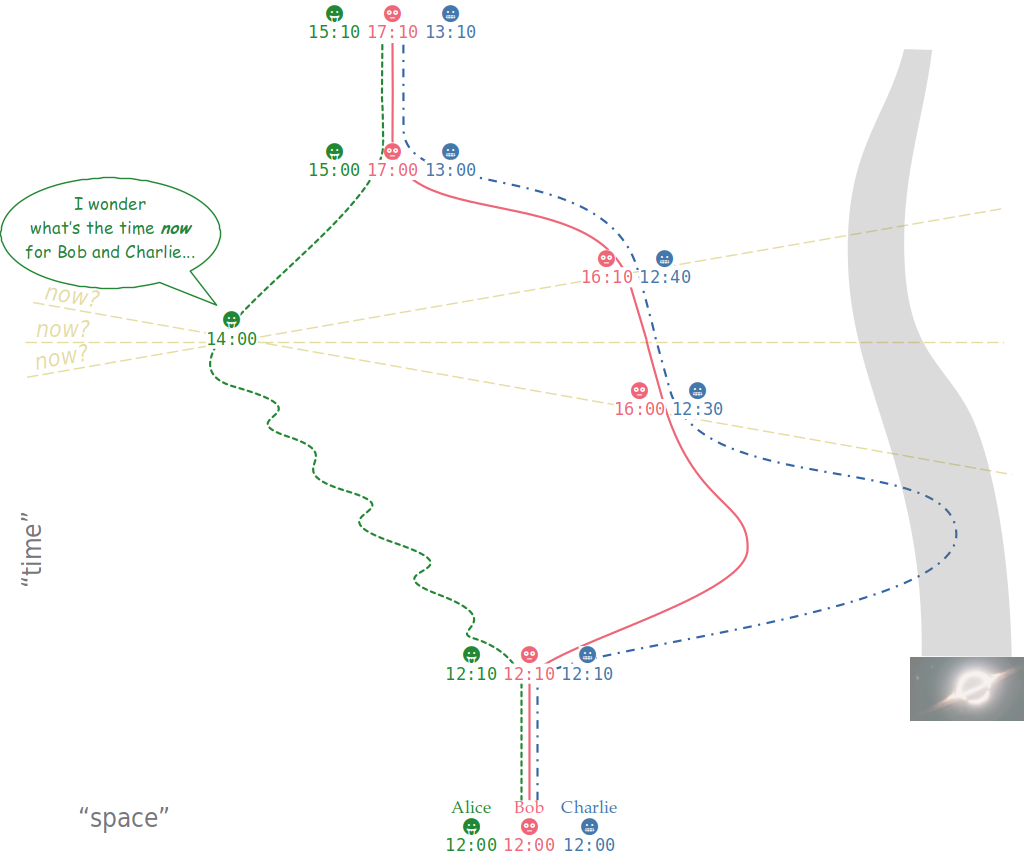
\includegraphics[width=\linewidth]{images/ABC_spacetime.png}
  \caption{Illustration of the experiences of Alice (\textcolor{green}{dashed \faIcon{grin-tongue}}), Bob (\textcolor{red}{solid \faIcon{flushed}}), Charlie (\textcolor{blue}{dot-dashed \faIcon{grimace}}) with time. The page represents a two-dimensional spacetime, and is read from bottom to top.
\\\textbf{Bottom}: Alice, Bob, Charlie stay close and observe their clocks are perfectly synchronized from 12:00 to 12:10, then they separate.
\\\textbf{Right}: Charlie visits a region near a strong \masse\ source. Upon meeting again with Bob, the two notice their clocks differ: 16:00 for Bob, 12:30 for Charlie. Yet this clock difference stays the same while they travel together for \qty{10}{min}.
\\\textbf{Left}: Alice wanders around travelling at high speed with respect to the fixed stars. At some point she wonders what's the time \enquote{now} for Bob and Charlie. Obviously this question doesn't make sense, because
(1)~when Bob and Charlie are together their clocks differ -- impossible to say what's \enquote{the} time at their position; (2)~not clear which instant in Bob \amp\ Charlie's trajectory should be considered as \enquote{now} (\textcolor{yellow}{yellow dashed lines}).
\\\textbf{Top}: When all three meet again, their clocks have completely different readings; and they themselves have aged differently. But their clocks run again at the same rate as long as they stay close.}  \label{fig:ABC_spacetime}
\end{figure}
%\clearpage

Consider for a moment an imaginary world in which these experiments had given a different kind of result. According to Newtonian mechanics, whenever two or more initially synchronized observers like Alice, Bob, Charlie were to meet again, their clocks would always show identical times. If one year, 23 days, 8 hours, 9 minutes, and \num{3.04539928324099266302} seconds had passed for Bob since he last met Alice, he would see that exactly the same amount of time had passed for Alice since their previous meeting. If you think about it, in this case it would have beeen somewhat natural for them to think \enquote{right now, the clock of far-away Charlie must show the same time as ours} (even though they have no real experimental way of confirming that).
% %
% \marginpar{\vspace{-2\baselineskip}\footnotesize\color{mpcolor}\enquote{\emph{%
% The plot for Cesium \textelp{} characterizes the best orbiting clocks in the GPS system. What this means is that after initializing a Cesium clock, and leaving it alone for a day, it should be correct to within \textelp{} 4~nanoseconds. Relativistic effects are huge compared to this.}}\sourceatright{\cites{ashby2003}}
% }
% %

But that's an imaginary world. In our world, what occurs is the more complicated situation with time discrepancies described initially. Only one conclusion can be drawn from these experimental results: \textbf{Time is not some sort of universal quantity. It is, so to speak, \enquote{local} to a person or clock, or to a group of persons or clocks that stick together.} This also means that \emph{it does not make sense} to ask questions like \enquote{what can be the time for far-away Charlie, \emph{right now}?}, or \enquote{what is happening at some other place \emph{right now}?}. The notion of \emph{now} is also local.


The time measured by a specific observer is called the \textbf{proper time} of that observer. Luckily we know more about how much the proper times of separated observers can differ when the observers meet again. According to our current understanding, it turns out that the time differences depend, roughly speaking, on how fast the observers are moving with respect to one another and with respect to the distribution of energy in the universe, and on how much energy is contained in the regions they travel across. The general theory of relativity gives us the equations determining any such proper-time differences. The more an observer's speed is close to the speed of light in vacuum $\yc$, a universal physical constant:
\begin{equation}
  \label{eq:c}
  \yc = \qty{299792458}{m/s}\quad\text{(exactly).}
\end{equation}

The situation depicted in our initial thought-experiment is real. Time discrepancies can be measured, for example, comparing initially synchronized clocks that have been put in aeroplanes flying in different directions. Most importantly, these time discrepancies affect everyday technologies such as the Global Positioning System. Formulae from General Relativity appear in your phone's GPS software; see for instance \sect\,20.3.3.3.3 of the Interface Control Document \texttt{IS-GPS-200} at \url{https://www.gps.gov/technical/icwg/}. Time discrepancies must also be taken into account in the establishment and synchronization of time in our everyday equipment:
\begin{quote}\footnotesize
  In 1976, the International Astronomical Union introduced relativistic concepts of time and the transformations between various time scales and reference systems. \textelp{} Now \textelp{} it is necessary to base all astrometry, reference systems, ephemerides, and observational reduction procedures on consistent relativistic grounds. This means that relativity must be accepted in its entirety, and that concepts, as well as practical problems, must be approached from a relativistic point of view.
  %
  \sourceatright{\parencites{kovalevskyetal2004}}
\end{quote}
%
% \marginpar{\vspace{-6\baselineskip}\footnotesize%
% \color{mpcolor}\enquote{\emph{In 1976, the International Astronomical Union introduced relativistic concepts of time and the transformations between various time scales and reference systems. \textelp{} Now \textelp{} it is necessary to base all astrometry, reference systems, ephemerides, and observational reduction procedures on consistent relativistic grounds. This means that relativity must be accepted in its entirety, and that concepts, as well as practical problems, must be approached from a relativistic point of view.}}\\{\cites{kovalevskyetal2004}}
% }

Note therefore the following curious situation. In setting up a time to meet a friend, you don't need to worry about the discrepancies between your and your friend's proper times: if your friend walks \qty{1000}{m} away from you and then immediately back to you, at \qty{1}{m/s}, then the time elapsed for you will be \qty{1000}{s} (around \qty{17}{min}), but the time elapsed for your friend will be \qty{999.999999999999994437}{s}. That's a difference of less than \qty{e-14}{s}, clearly negligible for the two of you, so you don't need to worry with General Relativity formulae in setting up your meeting time. Yet, if you set up a meeting place via GPS, then the true nature of time and General Relativity formulae become important: if they were not accounted for, you and your friend might end up off your meeting place by \qty{100}{m}.
% In most everyday situations for us, who live on or nearby Earth's surface and move at speeds much smaller than $\yc$ with respect to one another, the discrepancies between our proper times are so small that they cannot be measured with ordinary clocks or with our internal clocks. Consider a person walking \qty{10}{m} away from you and then immediately walking back to you, at \qty{1}{m/s}. The time elapsed for you will be \qty{20}{s}, but for that person will be \qty{19.999999999999999889}{s}, a difference of \qty{e-16}{s}, which is the error of an atomic clock. %%***add ref
% If human beings will still exist in some decades or centuries, in space travel they will have to deal with large proper-time discrepancies also in everyday life.

Luckily there's a way to bypass proper-time discrepancies: instead of referring to my proper time or to your proper time, we can agree on assigning a somewhat arbitrary time label to every event: this is called a \emph{coordinate time} and will be discussed in a couple of sections.
%
\marginpar{\vspace{-7\baselineskip}\centering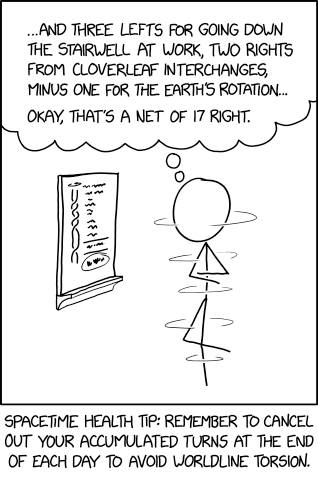
\includegraphics[width=\linewidth]{images/net_rotations.png} \\\footnotesize\color{mpcolor}%
  \url{https://xkcd.com/2882}%
}%
When we use coordinate time, some important physics formulae turn out to be the same no matter whether we use General Relativity or an approximate theory such as Newtonian Mechanics. Thanks to this fact, for the most part of these notes we will not need to deal with proper-time details. But I recommend that you keep in mind how time really works, and the small time discrepancies that exist and occur all the time along your \emph{worldline}.

\smallskip

Time has physical dimension of \textsf{time} and we shall for the most part measure it using the unit \emph{second}, symbol \enquote*{$\unit{s}$}.



\section{Space}
\label{sec:space}

Together with the notion of time, also the notion of space loses some of its traditional intuition. The first problem is that when we speak of the distance of an object, we mean the distance between us and the object \enquote{at the same instant of time}. But as we have seen, there is no correspondence between our \enquote{now} and the object's \enquote{now}. We could bypass this problem by specifying, say, \enquote{when our clock shows time $a$ and the object's clock shows time $b$}. Yet a second problem appears: traditionally, \enquote{distance} is measured along a \emph{straight line} between us and the object. But spacetime is curved. The closest notion to a \enquote{straight line} is that of a \furl{https://mathworld.wolfram.com/Geodesic.html}{\emph{geodesic}}. It turns out, however, that there may be several geodesics connecting us (at our time $a$) and the object (at its time $b$), and the distances along these geodesics may well be different.

Therefore the very notion of \enquote{distance} becomes tricky and has different and non-equivalent definitions. One must be very careful about which definition is being used. As a result, several observers in motion with respect to one another will generally disagree on the dimensions of an approximately rigid object in their vicinity. Luckily if the object is not too far away and if the speeds of the observers relative to one another are not too high, then all differently defined distances have very small discrepancies, and we can just speak of just one unique distance up to some precision. As an example, consider a car moving on a road at \qty{100}{km/h}, or around \qty{28}{m/s}. The car's driver may measure the length of the car to be \qty{4}{m}. A pedestrian that sees the car passing by may instead measure its length to be \qty{3.99999999999998}{m}, clearly a negligible and unmeasurable difference in many ordinary situations.
%
\marginpar{\vspace{-6\baselineskip}\centering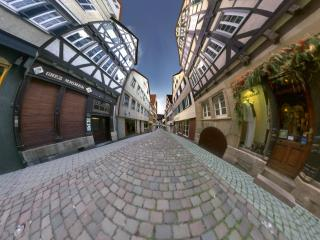
\includegraphics[width=\linewidth]{images/tuebingen.jpg}%
  \\[\jot]\footnotesize\flushleftright\color{mpcolor}How a street in T{\"u}bingen would look like (except for colour and some other features) if we travelled through it at around \qty{240000000}{m/s}. (From \furl{https://www.spacetimetravel.org/}{Relativity visualized}.)%
}%

These peculiarities of space and time also affect, at high speeds, how we \emph{see} objects. You can find beautiful visualizations, both static and animated, at \furl{https://www.spacetimetravel.org/}{Relativity visualized}.


\smallskip

We shall not delve further into these peculiarities of time and space. Keep simply in mind that phenomena happen in \textbf{spacetime}, and that there's no way to attribute a universal time, or a universal position in space, to a physical event. There is one absolute: whoever locally measures the speed of light in empty space, will find \autoref{eq:c}{the value $\yc$}. This value, exact by definition, serves as a way to define a local notion of space and distance.

\smallskip

Space has physical dimension of \textsf{length} and we shall for the most part measure it using the unit \emph{metre}, symbol \enquote*{$\unit{m}$}.


% In Bergen, a distance of 10\,m corresponds to a difference of 0.000\,1\,degree in latitude or longitude


\section{Coordinate systems and events}
\label{sec:coords}

We still need a way for distinguishing physical events and phenomena, and for locating them in spacetime. This is achieved through a \textbf{coordinate system}.

A coordinate system assigns four numerical labels to every point in spacetime.
%
\marginpar{\centering%
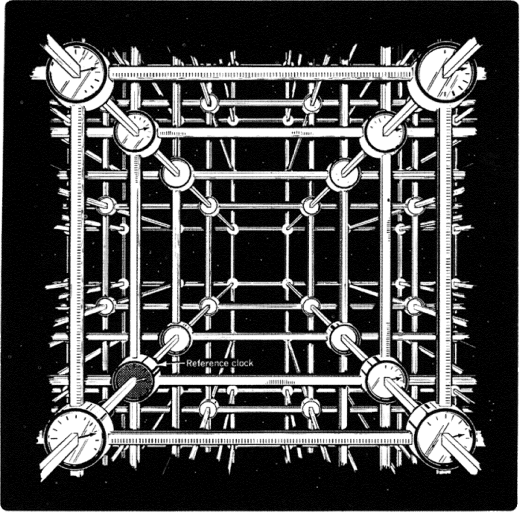
\includegraphics[align=t,width=\linewidth]{images/lattice_meters_clocks2.png}
\\[\jot]\footnotesize\flushleftright\color{mpcolor}%
A lattice of clocks and meters, defining a spacetime coordinate system (from \cites{tayloretal2000})%
}%
Often these labels have some kind of physical meaning -- like the proper time elapsed for a specific clock, or the distance from some event as measured by a specific observer -- but they don't need to.

A coordinate system solves the problem of proper-time and space discrepancies among different observers. To every physical event we assign, by agreement, a \emph{coordinate time} and a \emph{coordinate spatial position}. These coordinates are obviously the same for all observers, because they are decided by agreement. Coordinate time does not have a strict physical meaning, and will generally be different from the proper times measured by different observers. It can nevertheless be used for \enquote{doing physics}, and it is the time we shall most often use in our equations. A coordinate time commonly used for Earth-physics purposes is \furl{https://www.nist.gov/pml/time-and-frequency-division/time-realization/utcnist-time-scale-0/}{Universal Coordinated Time (UTC)}:
%\autocites[]{icwg1983_r2022}
\begin{quote}\footnotesize
  International Atomic Time (TAI) is based on more than 250 atomic clocks distributed worldwide that provide its stability, whereas a small number of primary frequency standards provide its accuracy. Universal Coordinated Time, which is the basis of all legal time scales, is derived from TAI. To allow the construction of TAI and the general dissemination of time, clocks separated by thousands of kilometres must be compared and synchronized. \textelp{} The achieved performances of atomic clocks and time transfer techniques imply that the definition of time scales and the clock comparison procedures must be considered within the framework of General Relativity. \sourceatright{\parencites{petitetal2005}}
%\mbox{}\hfill (\cites{petitetal2005})
\end{quote}
% \begin{figure}[h!]\footnotesize\centering%
% 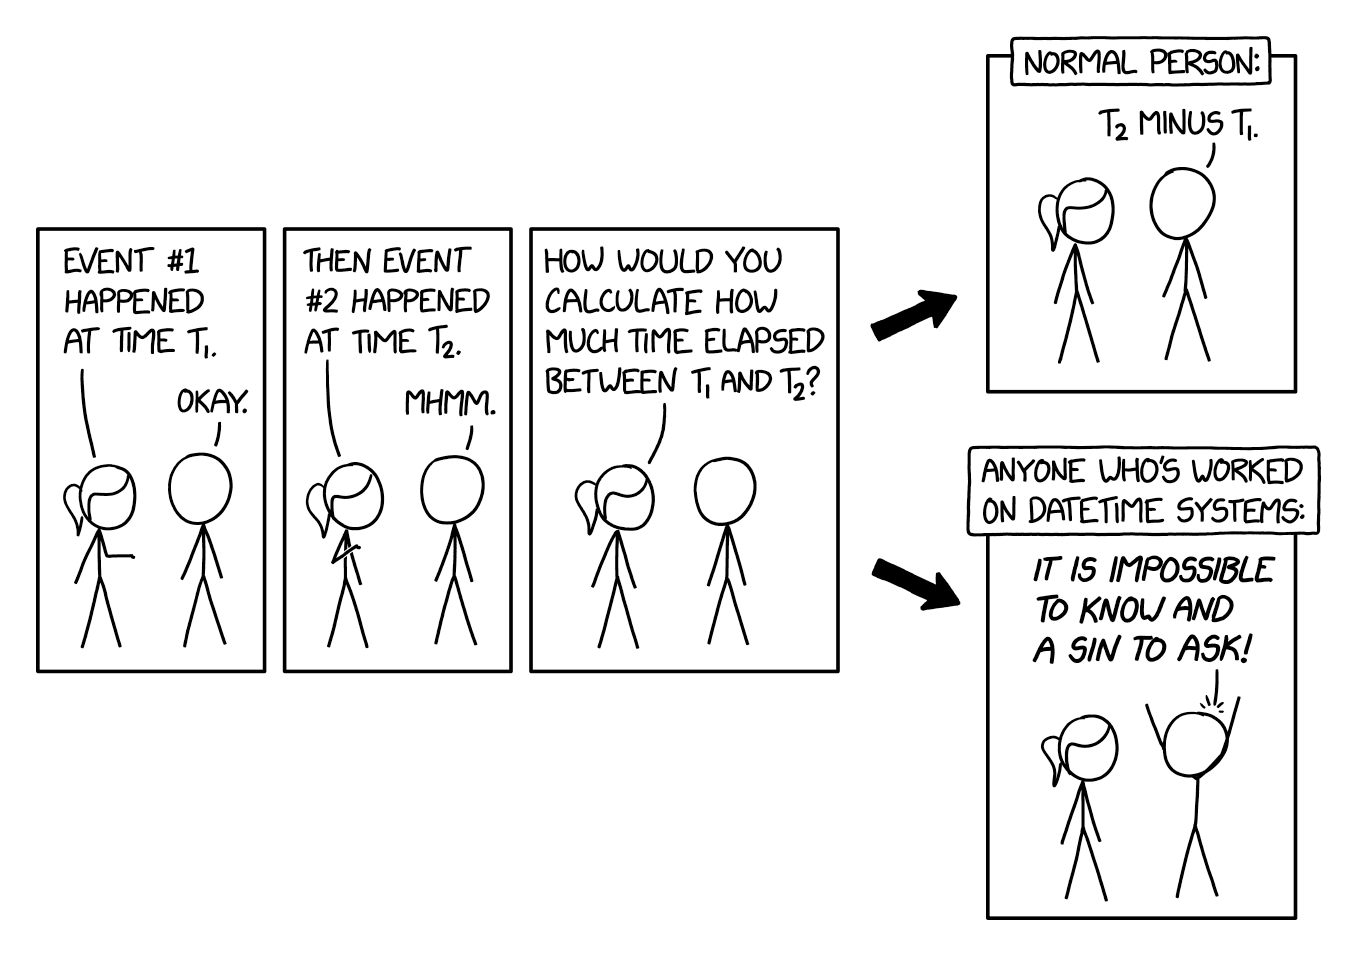
\includegraphics[align=t,width=0.75\linewidth]{images/datetime_2x.png}
% \\%
% \url{https://xkcd.com/2867}
% \end{figure}
The clock on your phone, and on devices synchronized via internet, shows UTC, not your proper time. An observer on Earth at \qty{0}{m} over sea level, and not moving, measures a proper time exactly equal to UTC (besides small variation coming from the movements of Solar System bodies). But observers at other altitudes and observers moving with respect to Earth's surface can measure that their proper times are slightly different from UTC.

Up to now we have often used the word \enquote*{event}, informally taking its meaning for granted. Let's be more precise: we call \textbf{event} or \textbf{spacetime point} an extremely small region of space -- a point -- that only lasts for a very small lapse of time -- an instant. The name \enquote*{event} is used because typically we approximately identify such a point and instant by means of a physical phenomenon of limited spatial extension and short duration, such as the collision of two subatomic particles. The sudden burst of a very small soap bubble can be considered as an event in some circumstances; but something like \enquote{a tennis ball} cannot be considered as an event, mainly because a tennis ball exists for quite a long time, not just for a short instant. From a four-dimensional spacetime point of view,
a tennis ball could be characterized as a line: a \textbf{worldline}.


\smallskip

We shall often denote the four coordinates of a coordinate system by the letters
\begin{equation*}
  (t, x, y, z)
\end{equation*}
where $t$ is a coordinate time, usually UTC, and $(x,y,r)$ determine a spatial position. The triplet of spatial coordinates is often denoted by the vector $\yr$:
\begin{equation*}
  \yr \defd (x,y,z)
  \qquad\text{or}\qquad
  \yr \defd [x,y,z]
  \qquad\text{or}\qquad
  \yr \defd
  \begin{bmatrix}
    x\\y\\z
  \end{bmatrix}
\end{equation*}
use round brackets \enquote*{$()$} or square brackets \enquote*{$[]$}, and horizontal or vertical notation as you prefer.

It is always important to specify how the coordinate system you're using is defined.
The definition of the spatial coordinates $(x,y,z)$ is typically different from problem to problem. We shall typically use coordinates that form $\frac{\pu}{2}\,\unit{rad} \equiv \ang{90}$ angles with one another; but their directions and their origin -- that is, where they have value $x=y=z=\qty{0}{m}$ -- always depend on the problem, so make sure you always specify them.

Whenever we speak of a \enquote{region of space} or of a \enquote{surface in space}, we mean a 3D or 2D region at some specific coordinate time $t$.

\smallskip

Some physical phenomena happen approximately along a line, in one dimension; or on a surface, in two dimensions. In these cases we can omit two or one of the spatial coordinates, assuming they have some constant, unimportant values; and we can simply write, for instance, $(t,x)$ or $(t,x,y)$ as our coordinates.

\begin{exercise}[label={ex:clocks}]
  Consider a clock at rest on the Earth's surface, at a distance $\color{green}r_{\text{e}}$ from the Earth's centre; and a clock on a satellite, for instance a GPS satellite or the \furl{https://www.nasa.gov/international-space-station/}{International Space Station}, right above the first clock, at a distance $\color{red}r_{\text{s}}$ from the Earth's centre. An observer by the clock on Earth measuring a time lapse $\Dt_{\text{e}}$ will see the clock on the satellite has having run for a time lapse $\Dt_{\text{s}}$, and vice versa (note that this \enquote{vice versa} only holds in this specific situation!). The relation between two time lapses is approximately given by
\sidepar{\centering%
  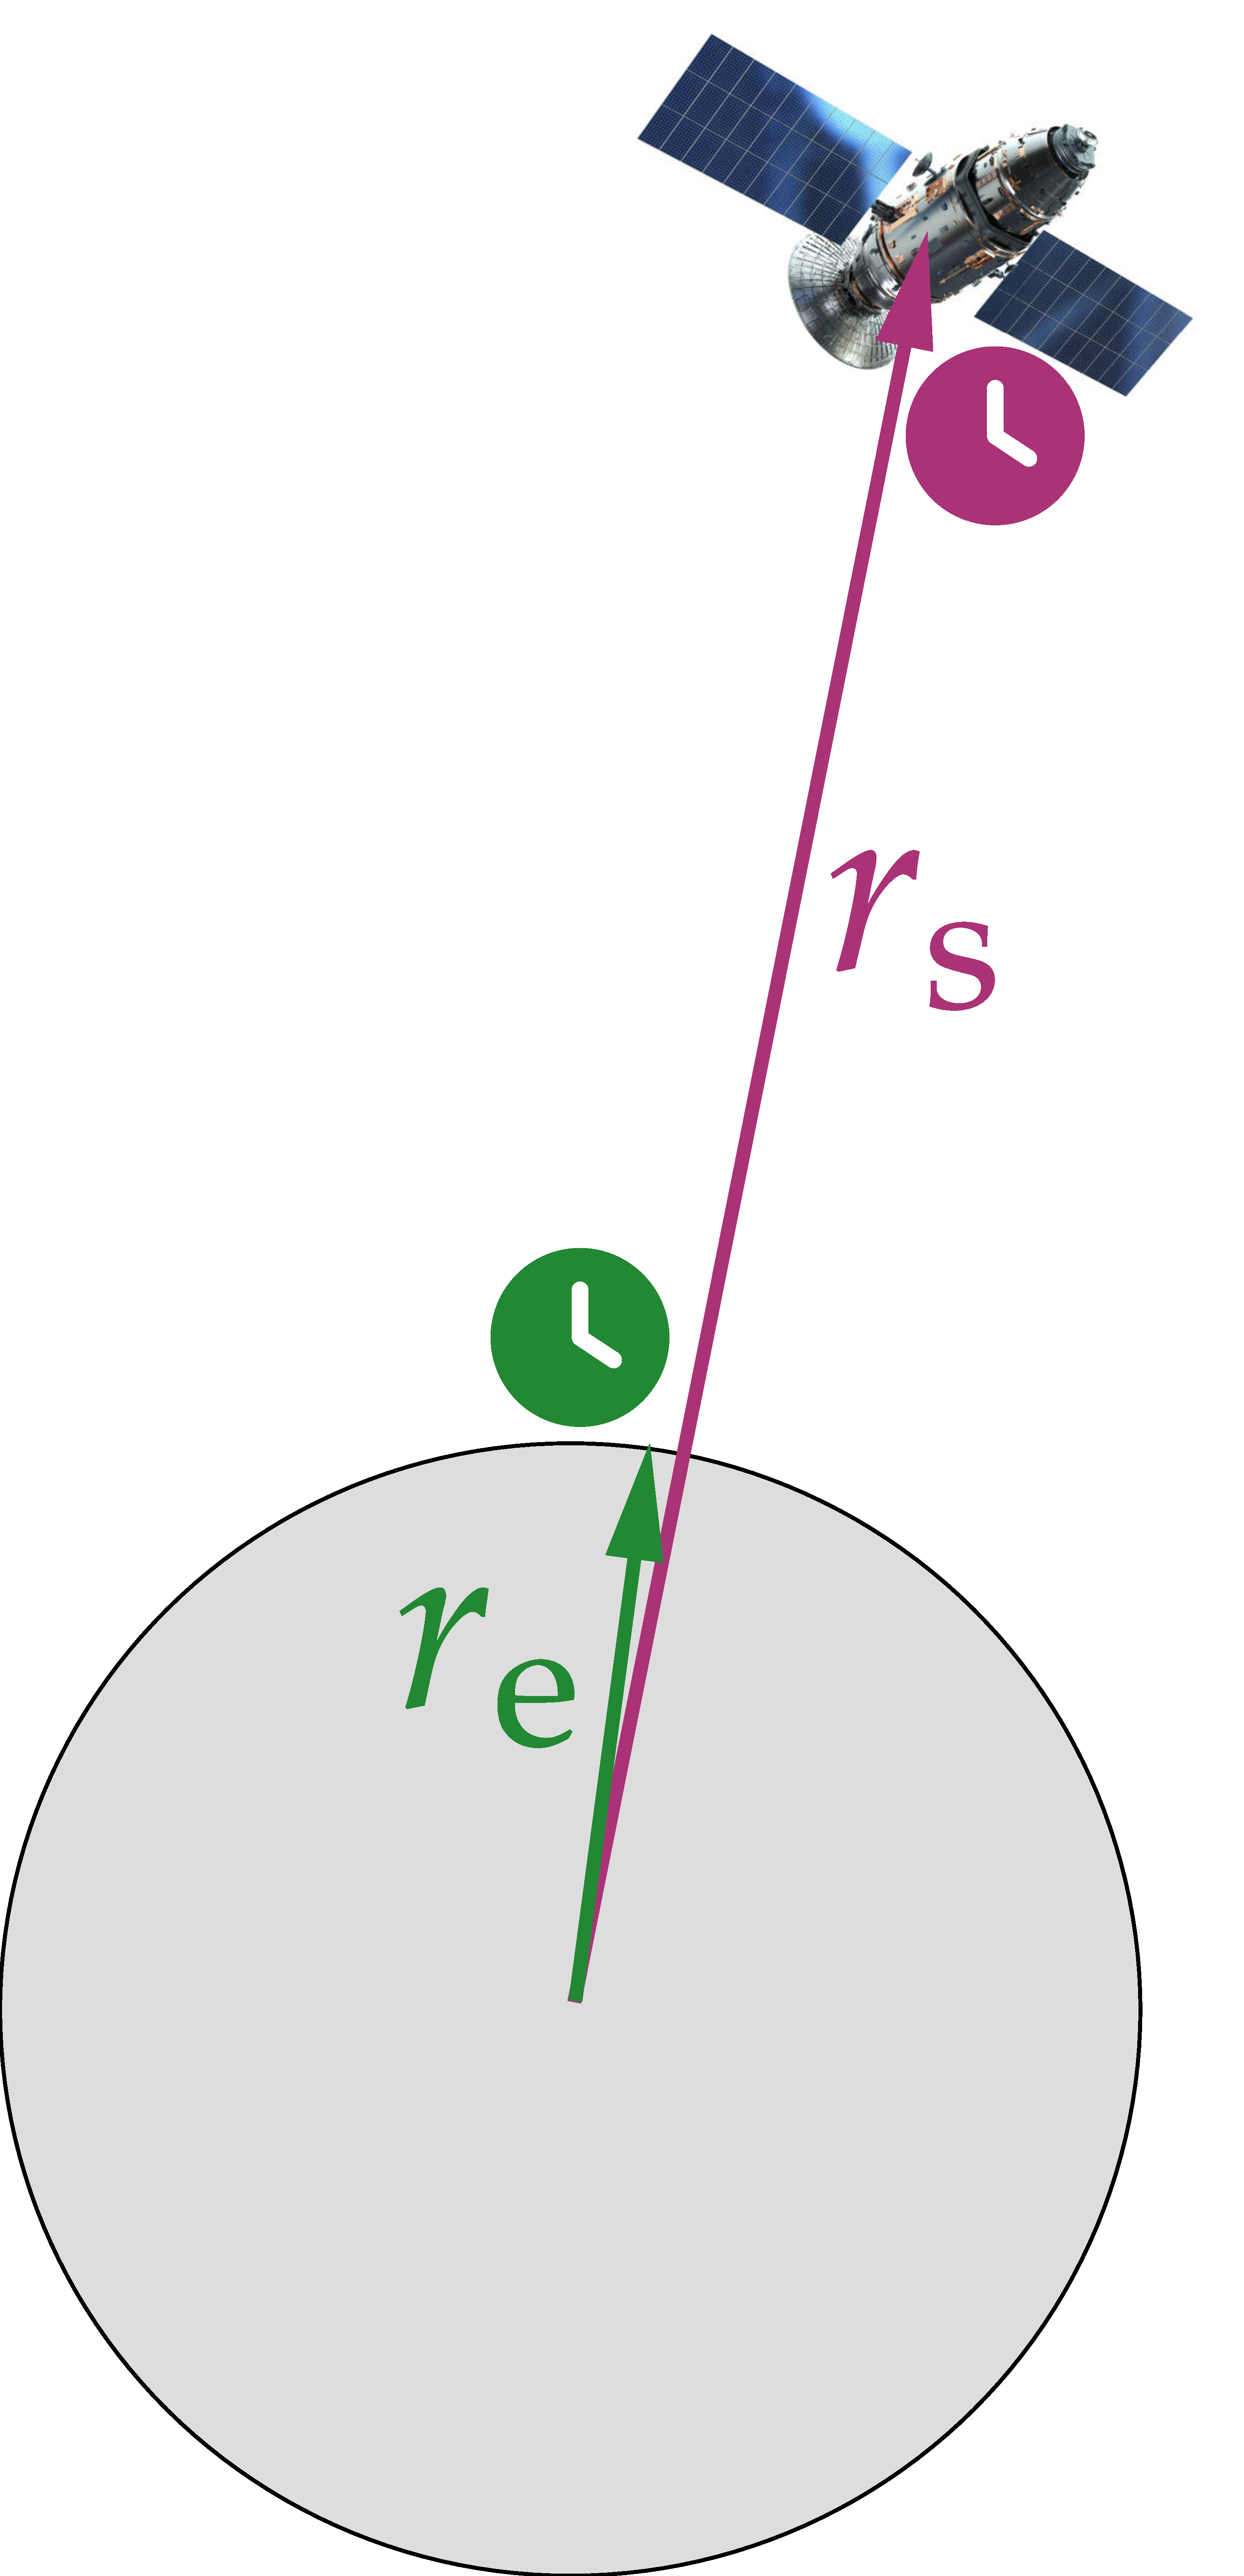
\includegraphics[align=t,width=0.75\linewidth]{images/re_rs.pdf}
}
\begin{equation*}
  \frac{\Dt_{\text{s}}}{\Dt_{\text{e}}} =
  \frac{
    \sqrt{1-2\frac{G}{c^{2}}\frac{M}{r_{s}}}
  }{
    \sqrt{1-2\frac{G}{c^{2}}\frac{M}{r_{e}}}
  }
\end{equation*}
where $G\approx\qty{6.7e-11}{m^{3}/(kg.s^{2})}$, $c=\qty{3.0e8}{m/s}$, and the Earth's mass $M=\qty{6.0e24}{kg}$.



\begin{enumerate}[exerc]
\item\label{item:gps_clock} Take the case of a GPS satellite, with $r_{\text{e}}=\qty{6.4e6}{m}$ and $r_{\text{s}}=\qty{2.6e7}{m}$ (\furl{https://www.nasa.gov/directorates/somd/space-communications-navigation-program/gps/}{NASA data}). If you, on the ground, measure a time lapse of $\Dt_{\text{e}}=\qty{10}{years}$, what's the difference, in seconds, with the time lapse $\Dt_{\text{s}}$ you see on the satellite?

\item\label{item:interstellar} If the time lapses are large compared with the time needed to go from ground to orbit or vice versa, then $\Dt_{\text{s}}/\Dt_{\text{e}}$ is also the ratio between the real \emph{ageing} of a person who's been in orbit and one who's been on the ground, when they meet again.

  Now consider the case with a black hole instead of Earth. The formula above can still be applied as an approximation.

  In the film \furl{https://www.imdb.com/title/tt0816692/}{\emph{Interstellar}}, two
  astronauts go on Miller's planet, at a distance $r_{\text{e}}$ from the black hole Gargantua, and stay there for \qty{3}{hours}, leaving one astronaut in orbit at a distance $r_{\text{s}}\approx \infty$ (the distance is large enough that it can be approximated as infinity). When they meet again, the latter astronaut has aged \emph{23\;years}.
\sidepar{\footnotesize\centering%
\vspace{-7em}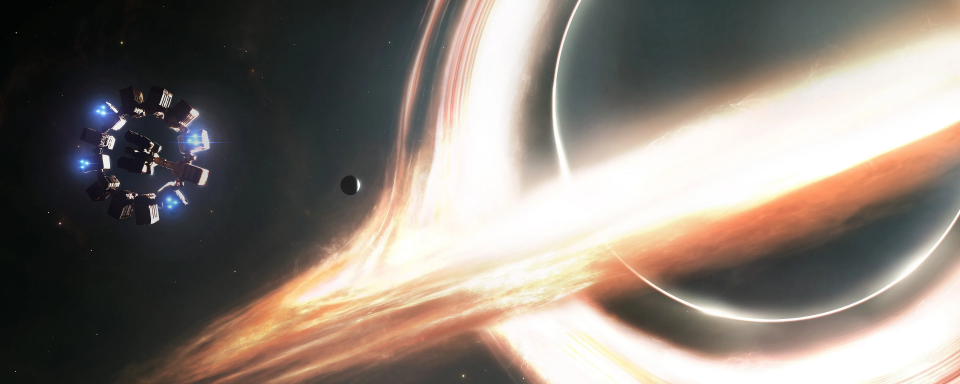
\includegraphics[width=\linewidth]{images/gargantua.png}
}

  Given that Gargantua's mass is $M=\qty{2.0e38}{kg}$, calculate the distance $r_{\text{e}}$ of Miller's planet from the black hole.
\end{enumerate}
\end{exercise}




\section{Velocity and acceleration}
\label{sec:velocity}

In some situations the spatial coordinates $\yr=(x,y,z)$ may turn out to be functions of the time coordinate $t$; the typical example is when we describe how the spatial position of a small body changes with coordinate time. We can write this functional dependence in different ways, for instance
\begin{equation*}
  \yr(t)\quad\text{or}\quad
  \bigl[x(t),\ y(t),\ z(t)\bigr] \ .
\end{equation*}
So $\yr$ is a vector function of time, which simply means that we have a collection of three functions of time.

If we take the derivative of each coordinate with respect to the time $t$, we obtain the \textbf{coordinate velocity}
\begin{equation*}
  \yv(t) \defd \frac{\di}{\di t}\yr(t) = \biggl[\frac{\di}{\di t} x(t),\ \frac{\di}{\di t} y(t),\ \frac{\di}{\di t} z(t)\biggr]
\end{equation*}
which is also a vector.

\begin{definition}{Dot-notation for time derivative}
  The derivative of some quantity with respect to coordinate time is often denoted by a \textbf{dot} over the quantity. So we can also write
  \begin{equation*}
    \yv(t) = \dot{\yr}(t) = \bigl[\dot{x}(t),\ \dot{y}(t),\ \dot{z}(t)\bigr]
  \end{equation*}
\end{definition}

The coordinate velocity is usually different from the \emph{physical velocity}, which an observer would measure using proper time and space, for instance using bouncing light rays. In many everyday situations the difference between coordinate and physical velocity is so small that it can be neglected. But in situations involving subatomic particles at high speed, for example, one must take into account that the two velocities are different.

\smallskip

Taking the time derivative once more we obtain the coordinate acceleration, also a vector:
\begin{equation*}
  \bm{a}(t) \defd \frac{\di}{\di t}\yv(t) =
  \frac{\di^{2}}{\di t^{2}}\yr(t) = \biggl[\frac{\di^{2}}{\di t^{2}} x(t),\ \frac{\di^{2}}{\di t^{2}} y(t),\ \frac{\di^{2}}{\di t^{2}} z(t)\biggr]
\end{equation*}
which is also a vector.

\begin{extra}{Acceleration in relativity theory}
  In relativity theory, acceleration acquires a special physical significance, because it includes the effect of gravity, and its calculation does not involve just a time derivative. For instance, let's say that you are standing still on the ground, and let's use a coordinate system where $x$ points in front of you, $y$ to your left, and $z$ points upwards. Then your coordinate velocity is $\yv=(0,0,0)\:\unit{m/s}$ also according to relativity theory. But the spatial part of your acceleration is approximately $(0,0,9.8)\:\unit{m/s^{2}}$, not zero!

  The definitions and values of acceleration according to relativity theory and according to Newtonian mechanics are therefore quite different even in everyday situations. In these notes we'll mean the Newtonian definition of acceleration, unless stated otherwise.
\end{extra}

\medskip

\begin{exercise}
  \begin{enumerate}[exerc]
  \item Here are the three components of a time-dependent velocity vector; the variable $t$ is the time, and therefore has dimension \textsf{time}. Introduce units \enquote*{\unit{s}} and \enquote*{\unit{m}} appropriately in such a way that the expression is dimensionally correct:
    \begin{equation*}
      \bm{v}(t) = \bigl[4, \cos(3\,t), -\exp(8/t)\bigr]
    \end{equation*}
  \item The position vector of a satellite is given below. Calculate the satellite's velocity and acceleration vectors:
    \begin{equation*}
      \yr(t) =
      \begin{bmatrix}
        \num[exponent-mode=scientific]{20e+6}\,
        \cos\bigl(\frac{t}{\qty{13751}{s}}\bigr)\\[2\jot]
        \num[exponent-mode=scientific]{22e+6}\,
        \sin\bigl(\frac{t}{\qty{13751}{s}}\bigr)\\[2\jot]
        \num{0}
      \end{bmatrix}\:\unit{m}
    \end{equation*}
  \item What is the satellite's velocity at $t=\qty{6875}{s}$? What is the magnitude of the velocity (that is, the speed)?
  \end{enumerate}
\end{exercise}


% \begin{subappendices}
%
% \addsec{\color{green}\faIcon{puzzle-piece}\enspace Exercises\enspace\faIcon{puzzle-piece}}
%
% % \setsecnumformat{E\upshape\oldstylenums{\csname the#1\endcsname\quad}}
% % \setsecnumformat{\sectionname\
% % \oldstylenums{\csname the#1\endcsname\quad}}
%
% \exsubsec{\ref{sec:coords}}
%
% \marginpar{\footnotesize\centering%
%   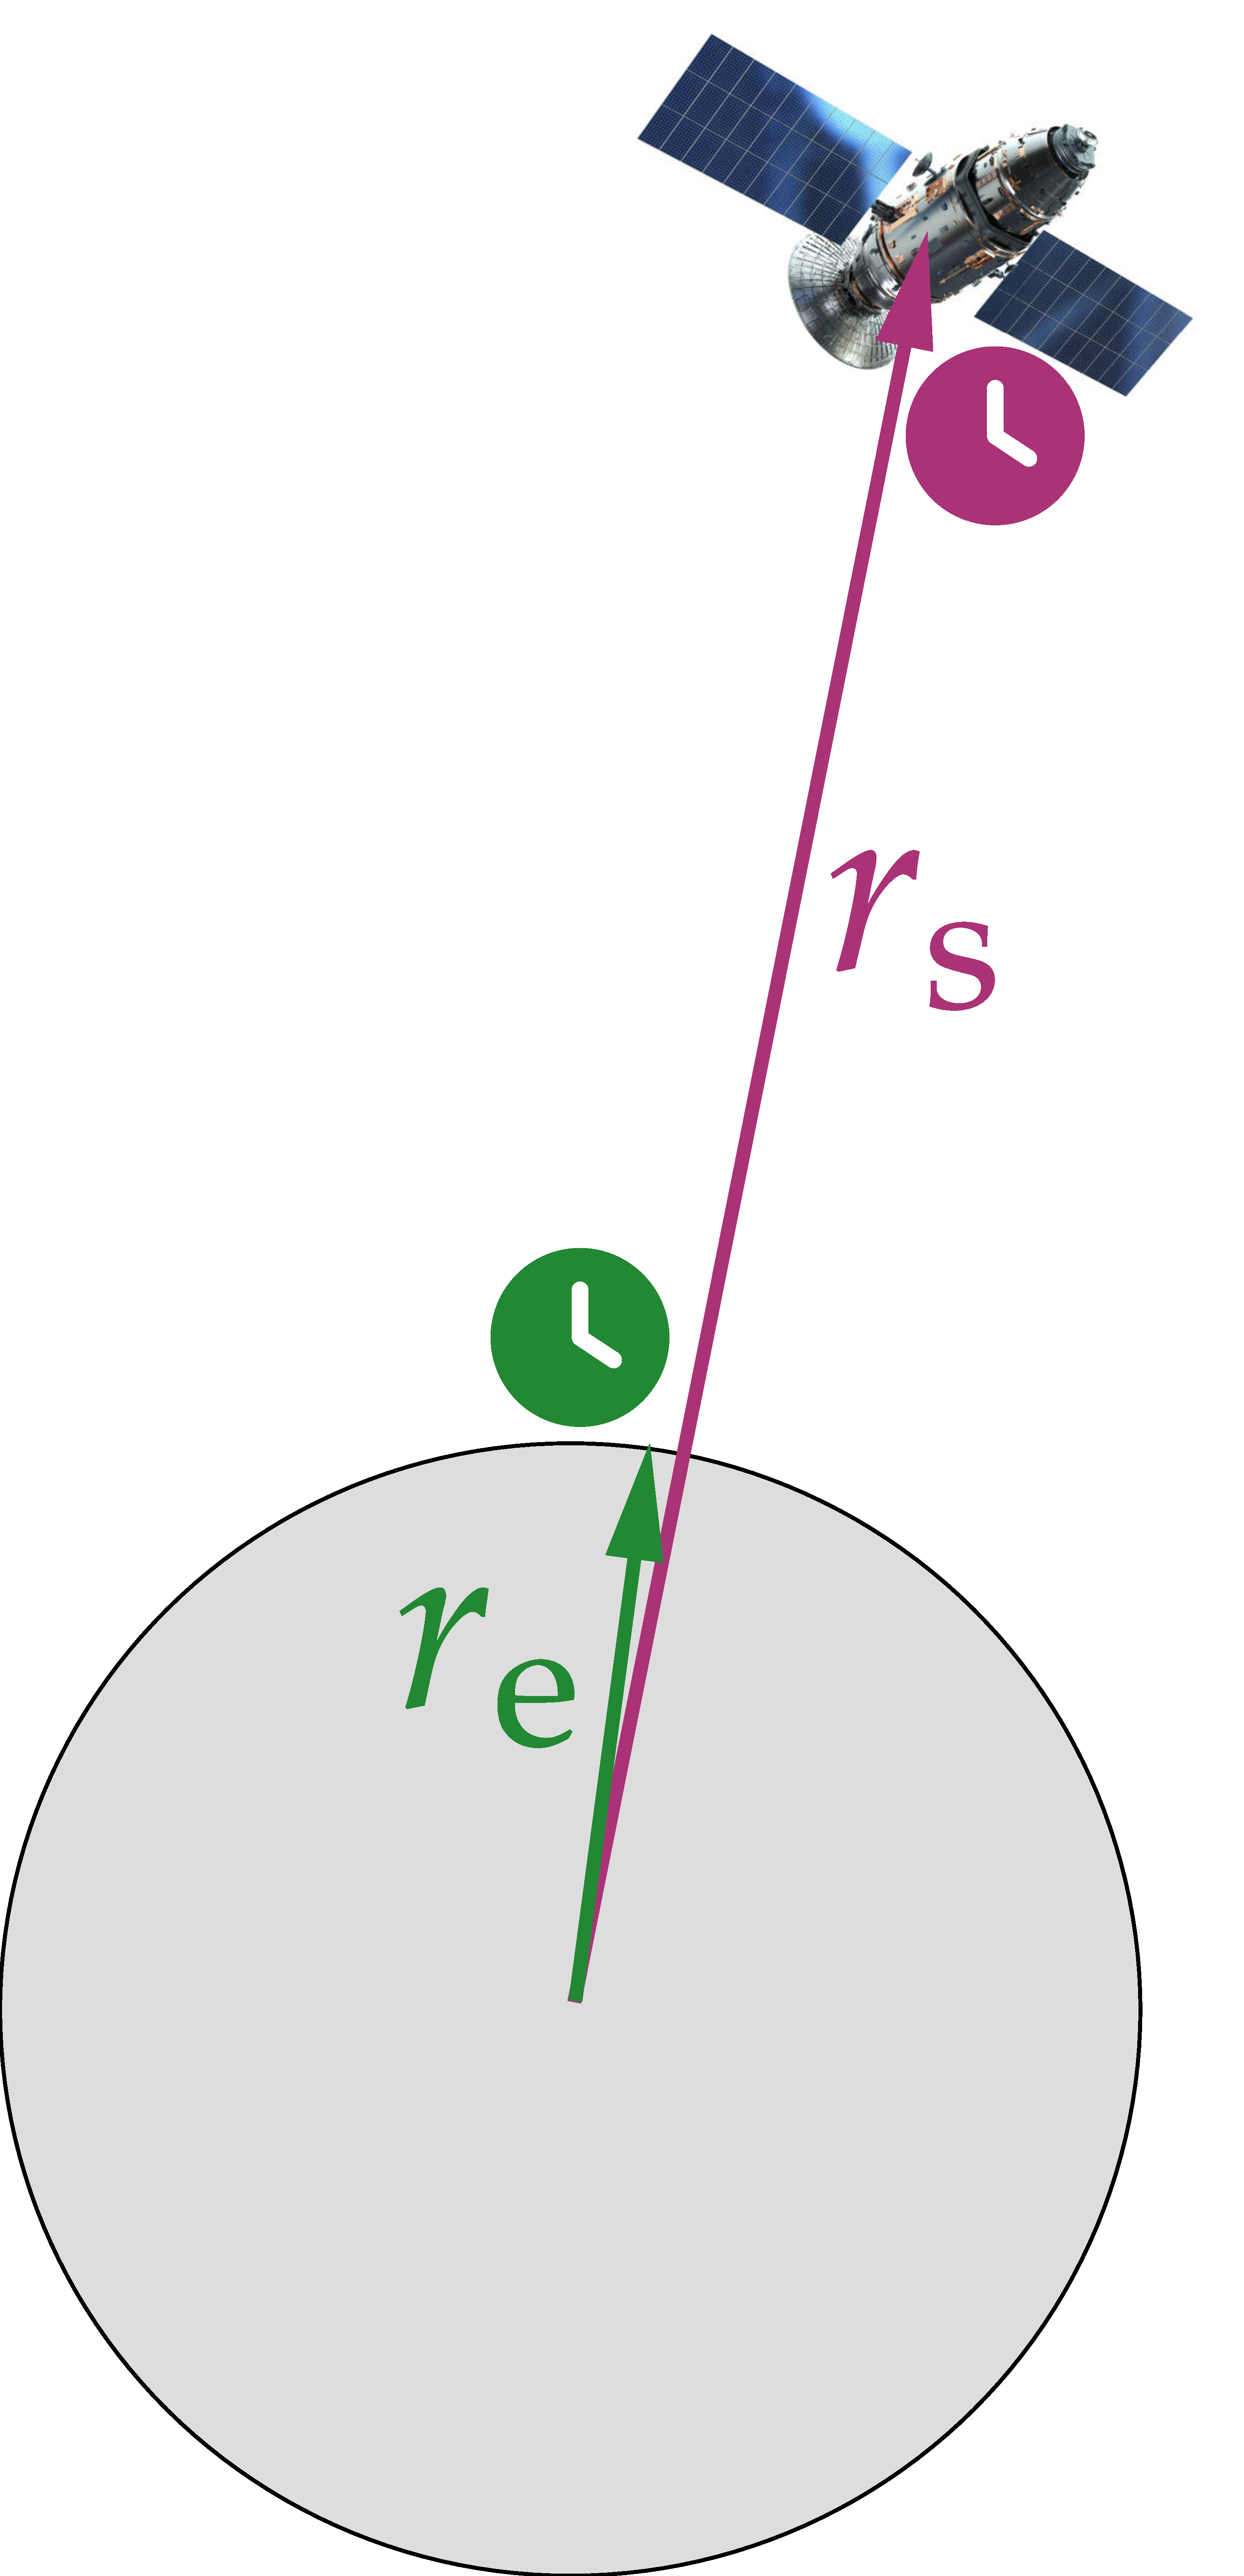
\includegraphics[align=t,width=0.75\linewidth]{images/re_rs.pdf}
% }
%   Consider a clock at rest on the Earth's surface, at a distance $\color{green}r_{\text{e}}$ from the Earth's centre; and a clock on a satellite, for instance a GPS satellite or the \furl{https://www.nasa.gov/international-space-station/}{International Space Station}, right above the first clock, at a distance $\color{red}r_{\text{s}}$ from the Earth's centre. An observer by the clock on Earth measuring a time lapse $\Dt_{\text{e}}$ will see the clock on the satellite has having run for a time lapse $\Dt_{\text{s}}$, and vice versa (note that this \enquote{vice versa} only holds in this specific situation!). The relation between two time lapses is approximately given by
% \begin{equation*}
%   \frac{\Dt_{\text{s}}}{\Dt_{\text{e}}} =
%   \frac{
%     \sqrt{1-\frac{G}{c^{2}}\frac{M}{r_{e}}}
%   }{
%     \sqrt{1-\frac{G}{c^{2}}\frac{M}{r_{s}}}
%   }
% \end{equation*}
% where $G\approx\qty{6.7e-11}{m^{3}/(kg.s^{2})}$, $c=\qty{3.0e8}{m/s}$, and the Earth's mass $M=\qty{6.0e24}{kg}$.
%
%
% \begin{enumerate}[exerc]
% \item Take the case of a GPS satellite, with $r_{\text{e}}=\qty{6.4e6}{m}$ and $r_{\text{s}}=\qty{2.6e7}{m}$ (\furl{https://www.nasa.gov/directorates/somd/space-communications-navigation-program/gps/}{NASA data}). If you, on the ground, measure a time lapse of $\Dt_{\text{e}}=\qty{10}{years}$, what's the difference, in seconds, with the time lapse $\Dt_{\text{s}}$ you see on the satellite?
%
% \item If the time lapses are large compared with the time needed to go from ground to orbit or vice versa, then $\Dt_{\text{s}}/\Dt_{\text{e}}$ is also the ratio between the real \emph{ageing} of a person who's been in orbit and one who's been on the ground, when they meet again.
%
%   Now consider the case with a black hole instead of Earth. The formula above still apply approximately.
%
%   In the movie \furl{https://www.imdb.com/title/tt0816692/}{\emph{Interstellar}}, two
%   astronauts go on Miller's planet, at a distance $r_{\text{e}}$ from the black hole Gargantua, and stay there for \qty{3}{hours}, leaving one astronaut in orbit at a distance $r_{\text{s}}\approx \infty$ (the distance is large enough that it can be approximated as infinity). When they meet again, the latter astronaut has aged \emph{23\;years}.
% \sidepar{\footnotesize\centering%
% \vspace{-10em}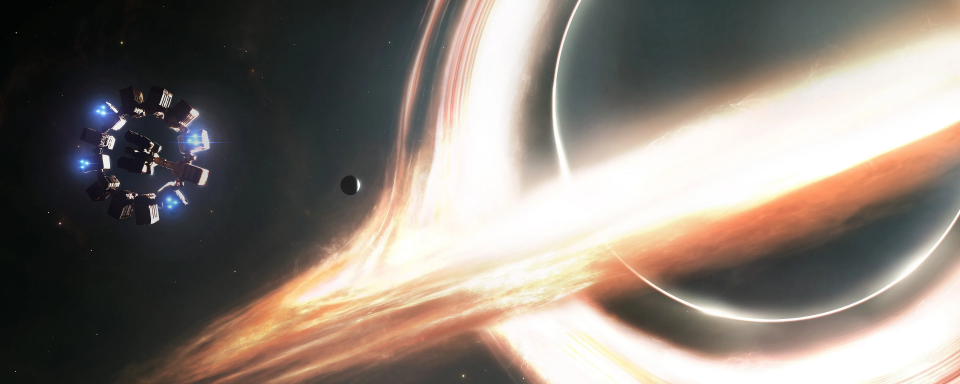
\includegraphics[width=\linewidth]{images/gargantua.png}
% }
%
%   Given that Gargantua's mass is $M=\qty{2.0e38}{kg}$, calculate the distance $r_{\text{e}}$ of Miller's planet from the black hole.
% \end{enumerate}
%
%
%
% \end{subappendices}





\printpagenotes*
\clearpage
\chapter{Main physical quantities}
\label{cha:stuff}

\epigraph{For Euler, clarity was the hallmark of truth. \textelp{} To him we owe also the brilliant imagination of the internal pressure in generality, the pressure field as equipollent to the action of the fluid outside any imaginary closed diaphragm upon that within. \textelp{} I remark upon it in emphasis of the role of imagination and the importance of quantities which can only be thought of and cannot in themselves be measured.}{C. A. Truesdell \cites*{truesdell1956d}}

% \epigraph{if the skill of the mathematician has enabled the experimentalist to see that the quantities which he has measured are connected by necessary relations, the discoveries of physics have revealed to the mathematician new forms of quantities which he could never have imagined for himself.}{J. Clerk Maxwell \cites*{maxwell1870}}


\section[Seven primitive quantities]{Seven primitive quantities: basic properties}
\label{sec:stuff}

Besides time and space, our physics formalism includes seven more quantities that we take as primitive:
\begin{definition}{Seven primitive quantities}
  \begin{center}\bfseries
    matter
    \\ electric charge
    \\ magnetic flux
    \\ energy
    \\ momentum
    \\ angular momentum
    \\ entropy
  \end{center}
\end{definition}
% Technically they are called \emph{fields}, for reasons we shall shortly see.

\medskip

Recall that primitive quantities cannot be defined: we can only try to understand them intuitively. Some of the seven primitive quantities are easier to grasp intuitively than others. But all seven primitive quantities have three basic properties in common:

First of all, for each quantity except the magnetic flux we can ask or measure:
\begin{definition}{The two basic measurements that can be made on the seven quantities}
  \begin{enumerate}[shift,label=\arabic*.]\bfseries
  \item How much of this quantity is in a particular three-dimensional region of space at a particular time instant?

  \item How much of this quantity flows through a particular two-dimensional surface during a particular time lapse?
  \end{enumerate}
\end{definition}
We can ask these questions of any region of space and any time lapse, and the surface in the second question can be moving and deforming. The results of the two measurements above are either (positive or negative) numbers, for scalar quantities; or vectors, for vector quantities.
% This number depends only on the chosen region, surfaces, and times.

We can consider the question about the flow through a surface in the case of a very short lapse of time, and divide the total flow by that lapse. This way we have an alternative form of the second measurement, as flow per unit time:
\begin{definition}{Flux of a substance through a surface}
  \begin{enumerate}[shift,label=\arabic*.]\bfseries
  \item[2b.] How much of this quantity is flowing through a particular two-dimensional surface per unit time, at a particular time instant?
  \end{enumerate}
\end{definition}
This is called the \textbf{flux} of the quantity through that surface.

The third property common to all seven quantities tells how the measurements above combine for several regions of space and several surfaces: by simple addition:
\begin{definition}{Extensivity of the seven quantities,label={def:extensivity}}
\begin{enumerate}[shift,label=\arabic*.]\bfseries
  \item[3.]  If we consider two or more non-overlapping volumes, the amount of quantity in the total volume is equal to the sum of the amounts in the separate volumes.

    If we consider two or more non-overlapping surfaces, the amount of quantity flowing through the total surface is equal to the sum of the amounts flowing through the separate surfaces.
  \end{enumerate}
\end{definition}
We say that each of the seven quantities is an \textbf{extensive} quantity.

We shall later see that analogous properties hold for the magnetic flux, the only difference being that instead of holding in 3 and 2 dimensions, they hold in 2 and 1 dimensions.

\smallskip

The basic measurements above can't in general be made, and don't even make sense, for some other quantities. For instance, we cannot ask \enquote{what's the total amount of temperature in this region?}, or \enquote{how much velocity is flowing through this surface?}.

\smallskip

Thanks to the three properties above, each of the seven quantities can be intuitively visualized as some kind of \enquote{stuff} that fills regions of space or flows through surfaces. This visualization is useful, but also comes with some warnings which we shall discuss later.
% But don't take the word \enquote*{stuff} too literally: I don't necessarily mean concrete objects like a ball, or substances like water.

% For each quantity, we can speak of its \emph{density}, in relation to the question \enquote{how much of it is in a particular region?}; and of its \emph{flux}, in relation to the question \enquote{how much of it flows through a surface during some time?}. The density tells us how much quantity there's in a unit of volume. The flux tells us how much quantity is flowing through a unit of surface in a unit of time. Density and flux can change from spacetime point to spacetime point. We shall discuss them more in detail for each quantity later on. One important aspect to keep in mind is that \emph{the density and flux of each quantity depend on the coordinate system}.

\medskip

What's remarkable about matter, electric charge, magnetic flux, energy, momentum, angular momentum, and entropy, is that \emph{they are common to all our main physical theories}, approximate or not: from Newtonian mechanics to General Relativity and quantum theory; from subatomic scales to cosmological scales. And in all these theories they possess the three basic properties discussed above. The physical meaning and mathematical characterization of these quantities can be slightly different depending on the physical theory and spatial or temporal scale. For example, in quantum theory they are mathematically represented by so-called operators rather than functions; and at molecular scales entropy has a meaning connected with probability theory. Yet, these seven quantities are universal in our present way of doing physics and of describing and understanding physical phenomena all around and within us.

% \begin{critique}
%   \emph{Wait! what about \emph{force}? isn't this a primitive quantity? or maybe it isn't included because it's defined as mass${}\times{}$acceleration?}
%
%   \smallskip
%
% We'll see that \emph{force} is defined as momentum flux; but that in general isn't mass${}\times{}$acceleration.
% \end{critique}

Let us make a first acquaintance with these seven quantities. The discussion that follows is meant as an introduction; we shall repeat and say more about each quantity in later chapters.
%
\marginpar{\vspace{-6\baselineskip}\centering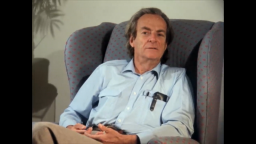
\includegraphics[width=\linewidth]{images/feynman_why2.png}%
\\[\jot]\footnotesize\flushleftright\color{mpcolor}%
Richard Feynman explains the difficulty of \enquote{why} questions in a \furl{https://www.youtube.com/watch?v=nYg6jzotiAc&t=893s}{funny and insightful video}.%
}%
But keep in mind that it is very difficult, if not impossible, to answer questions like \enquote{what \emph{really} is the quantity\textellipsis?}

\section{Matter}
\label{sec:intro_matter}

Matter is a \emph{scalar} quantity, with SI dimension \furl{https://doi.org/10.1351/goldbook.A00297}{\textsf{amount of substance}}, and measured in \furl{https://doi.org/10.1351/goldbook.M03980}{\emph{moles} (\unit{mol})}. Its flux is therefore measured in \emph{moles per second} (\unit{mol/s}). In statistical mechanics and particle physics, matter is often simply counted and so measured in dimensionless units, rather than moles.

\smallskip

Matter is probably the easiest quantity to grasp intuitively: it is what we ordinarily call \enquote{stuff}. % It is called \furl{https://doi.org/10.1351/goldbook.C01039}{\emph{chemical substance}} in chemistry, and \emph{baryons} and \emph{leptons} in particle physics.
It is usually classified into several kinds. The classification depends on the physical phenomena and theory one works with.

A building engineer, for instance, could classify \enquote{matter} into different kinds of \emph{materials} -- such as wood, concrete, steel, sand, plastic, and so on -- keeping track of the amount of each material in different regions of space, its movement, its rate of production and transformation. Each material has different physical properties.

A chemist could classify matter into different \emph{substances} -- such as water, hydrogen, oxygen, carbon dioxide, and so on -- again keeping track of their amounts, movements, production. According to this classification, the \enquote{materials} of the building engineer would be mixtures of the different substances. But note that there is no clear boundary between one classification and the other.

A chemist could also classify matter into different kinds of \emph{atoms} -- such as \furl{https://pubchem.ncbi.nlm.nih.gov/element/Hydrogen}{hydrogen}, \furl{https://pubchem.ncbi.nlm.nih.gov/element/Helium}{helium}, \furl{https://pubchem.ncbi.nlm.nih.gov/element/Lithium}{lithium}, and the other kinds that appear in the \furl{https://iupac.org/what-we-do/periodic-table-of-elements/}{periodic table} -- and seeing substances and materials as combinations of these different atomic kinds of matter. This classification is special because these different kinds have, at least approximately, the property of being \autoref{sec:balance_intro}{conserved}: their amounts in a container or in a region of space can only change if these kinds are entering through an opening in the container or through the boundary of the region of space. In other words, they cannot be created or destroyed. This conservation property is only approximate, however. \furl{https://www.ciaaw.org/radioactive-elements.htm}{Radioactive atoms} can transmute from one kind to another. This possibility is crucial and must be taken into account in phenomena involving \furl{https://www.iaea.org/newscenter/news/what-are-radioactive-sources}{radioactivity}
% \url{https://www.britannica.com/science/radioactivity}
and \furl{https://www.iaea.org/newscenter/news/what-is-nuclear-energy-the-science-of-nuclear-power}{nuclear energy}.

A chemist or a particle physicist may classify matter into fewer different kinds: protons, neutrons, electrons, anti-protons, anti-neutrons, anti-electrons (also called \emph{positrons}), seeing the different atomic kinds as being made of these six basic ones. These kinds may be conserved even when kinds of atoms are not.

But a nuclear or particle physicist knows that the conservation properties of the six kinds above is also only approximate, and there are also other kinds, produced only in special circumstances.

We therefore go down into more and more subtle classifications. This kind of research is still open, but it seems that the total amount of \furl{http://hyperphysics.phy-astr.gsu.edu/hbase/Particles/hadron.html\#c6}{\emph{baryonic}},
% \url{https://www.britannica.com/science/baryon}},
(including protons and neutrons) and \furl{http://hyperphysics.phy-astr.gsu.edu/hbase/Particles/lepton.html\#c1}{\emph{leptonic}} (including electrons) matter is always conserved.
% \url{https://www.britannica.com/science/lepton}},

\medskip

According to the definition of matter that we're adopting, the total amount of some kind of matter in a region can in principle be \emph{negative}. A negative amount simply denotes the presence of \furl{https://www.britannica.com/science/antimatter}{anti-matter}. Anti-matter appears in small amounts in everyday life, for example in connection with common radioactivity processes. It is also created and used in medicine, in \furl{https://www.britannica.com/topic/positron-emission-tomography}{positron-emission tomography (PET)} scans. In ordinary chemical applications, however, all amounts of matter within a region are usually positive or zero.
%
\marginpar{\vspace{-5\baselineskip}\centering%
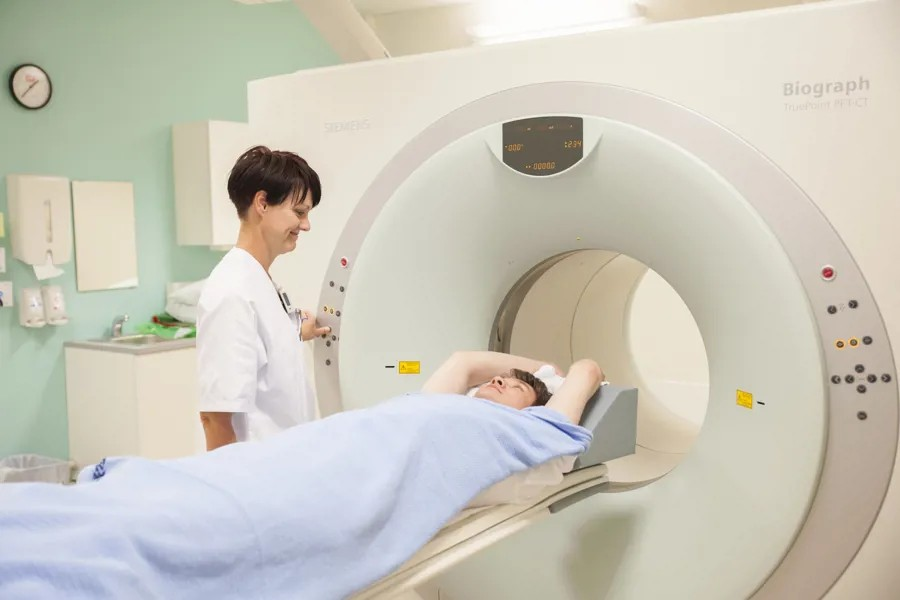
\includegraphics[width=\linewidth]{images/pet_scan_bergen.jpg}%
\\[\jot]\footnotesize\flushleftright\color{mpcolor}%
In positron-emission tomography there is creation of amounts of matter (leptonic matter) that can be considered negative: their \emph{lepton number} is negative (\furl{https://www.helse-bergen.no/avdelinger/radiologisk-avdeling/senter-for-nukleermedisin-og-pet/tilvising-til-pet}{image: Helse Bergen}).%
}%

\medskip

Why do we need to worry about how matter gets classified depending on the application? Because for describing a physical system and predicting its behaviour we usually have to use at least one physical law \emph{for each kind of matter}. So the more kinds of matter we have to keep track of, the more equations we will have.



\begin{definition}{Matter: notation}
  The amount of matter in a region is usually denoted with $\yN$, and flux of matter with $\yJ$. In chemistry we usually specify what kind of matter we are speaking about, writing for instance $\yN_{\mathrm{Ca}}=\qty{5.3}{mol}$, to indicate an amount of $\qty{5.3}{mol}$ of \furl{https://pubchem.ncbi.nlm.nih.gov/element/Calcium}{calcium} atoms.
\end{definition}



\begin{warning}[Ambiguity of the term \enquote*{matter}]
In these notes we use the term \enquote*{matter} in a the generic sense discussed above. But be aware that in specialized applications, this term may have a much more specialized and slightly different meaning. It may even \emph{not} be used at all. In chemical applications, for instance, one typically speaks specifically of \enquote*{compounds}, \enquote*{mixtures}, \enquote*{substances}, \enquote*{elements}, rather than \enquote*{matter}. A particle physicists speaks of \emph{matter} and \emph{anti-matter}, but in the present notes the term \enquote*{matter} refers to both.
\end{warning}


% In these notes we shall usually not consider distinctions between different kinds of matter, making some exceptions for discussions about chemical reactions and nuclear phenomena.

% There are different kinds of matter The distinction into different kinds depends on the physical theory. In most everyday situations, the distinction corresponds to different \furl{https://doi.org/10.1351/goldbook.C01022}{chemical elements}, and each satisfies its own balance. These balances are the basis of \furl{https://doi.org/10.1351/goldbook.S06026}{stoichiometry}. If we observe phenomena like nuclear fission or fusion, however, we notice that the balances of chemical elements are not really satisfied. With such phenomena we make a different distinction of types of matter, for instance \emph{baryons} and \emph{leptons}, and each satisfies again its own balance. It is unclear whether these balances might be broken in other physical phenomena at smaller scales. In these notes we shall usually consider chemical elements as the different kinds of matter, making some exceptions in discussion of nuclear phenomena.

\begin{warning}[Matter is different from mass or energy]
  It is important to clearly distinguish matter from \emph{mass} or \emph{energy}. Mass can be considered a property of matter, but the two are different. In nuclear reactions, for instance, the mass of some amount of matter may change, even if the amount of matter stays the same.

  \smallskip

  As far as we know, the total amount of energy associated with an amount of matter is always positive, whether the amount of matter is positive or negative (antimatter). This is the reason why antimatter \enquote{falls} just like positive matter, a fact that has been experimentally confirmed: see \cites{andersonetal2023}.
\end{warning}

\begin{exercise}
  According to statements on \furl{https://www.symmetrymagazine.org/2009/07/23/antimatter-from-bananas}{symmetrymagazine.org} and \furl{https://www.quantumdiaries.org/2009/07/21/positrons-from-bananas/}{quantumdiaries.org},
  \begin{quote}
    The average banana (rich in potassium) produces a positron roughly once every 75 minutes.
  \end{quote}
  Unfortunately the original site where the this statement was discussed, and the corresponding calculation made, seems not to exist anymore.

\begin{enumerate}[exerc]
\item Do a little research and find out whether this statement is true.
\item From your research, approximately quantify the flux of positrons around an ordinary banana, expressing it in \unit{particles/s}.
\end{enumerate}
\end{exercise}
\marginpar{\vspace{-15em}\footnotesize%
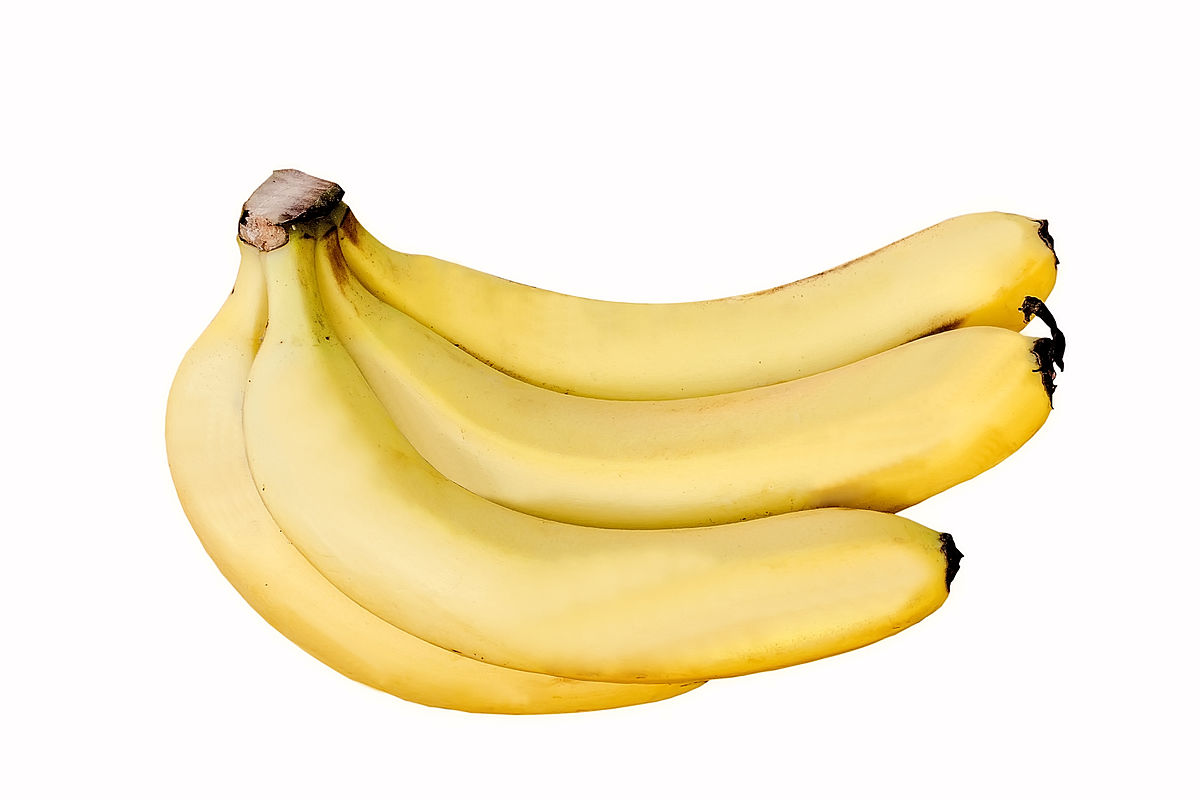
\includegraphics[width=\linewidth]{images/banana.jpg}
\\\color{mpcolor}How many positrons do bananas produce?%
}



\section{Electric charge}
\label{sec:intro_charge}

Electric charge is a \emph{scalar} quantity, with SI dimension \furl{https://doi.org/10.1351/goldbook.E01923}{\textsf{electric charge}} (equivalent to \textsf{electric current}$\times$\textsf{time}), and measured in units of \furl{https://doi.org/10.1351/goldbook.C01365}{\emph{coulombs} (\unit{C})}. Flux of electric charge is called \emph{electric current}, and measured in units of \furl{https://doi.org/10.1351/goldbook.A00300}{\emph{amperes} ($\unit{A} = \unit{C/s}$)}.

Electric charge is a quantity that is easily grasped in our everyday experience, and doesn't need much comments.

\mynotew{To be completed in a later version}



\section{Magnetic flux}
\label{sec:intro_charge}


\marginpar{\vspace{-3\baselineskip}\centering%
%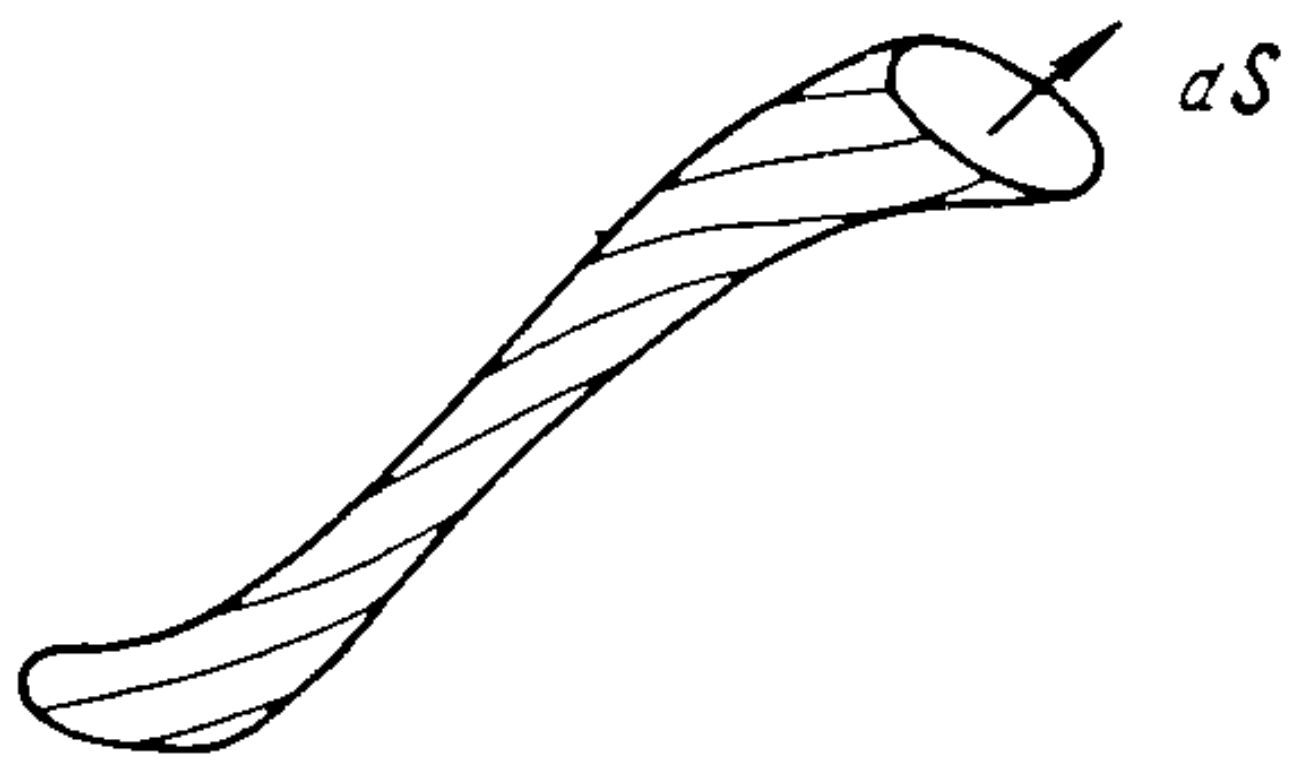
\includegraphics[align=t,width=\linewidth]{images/magnflux1.png}
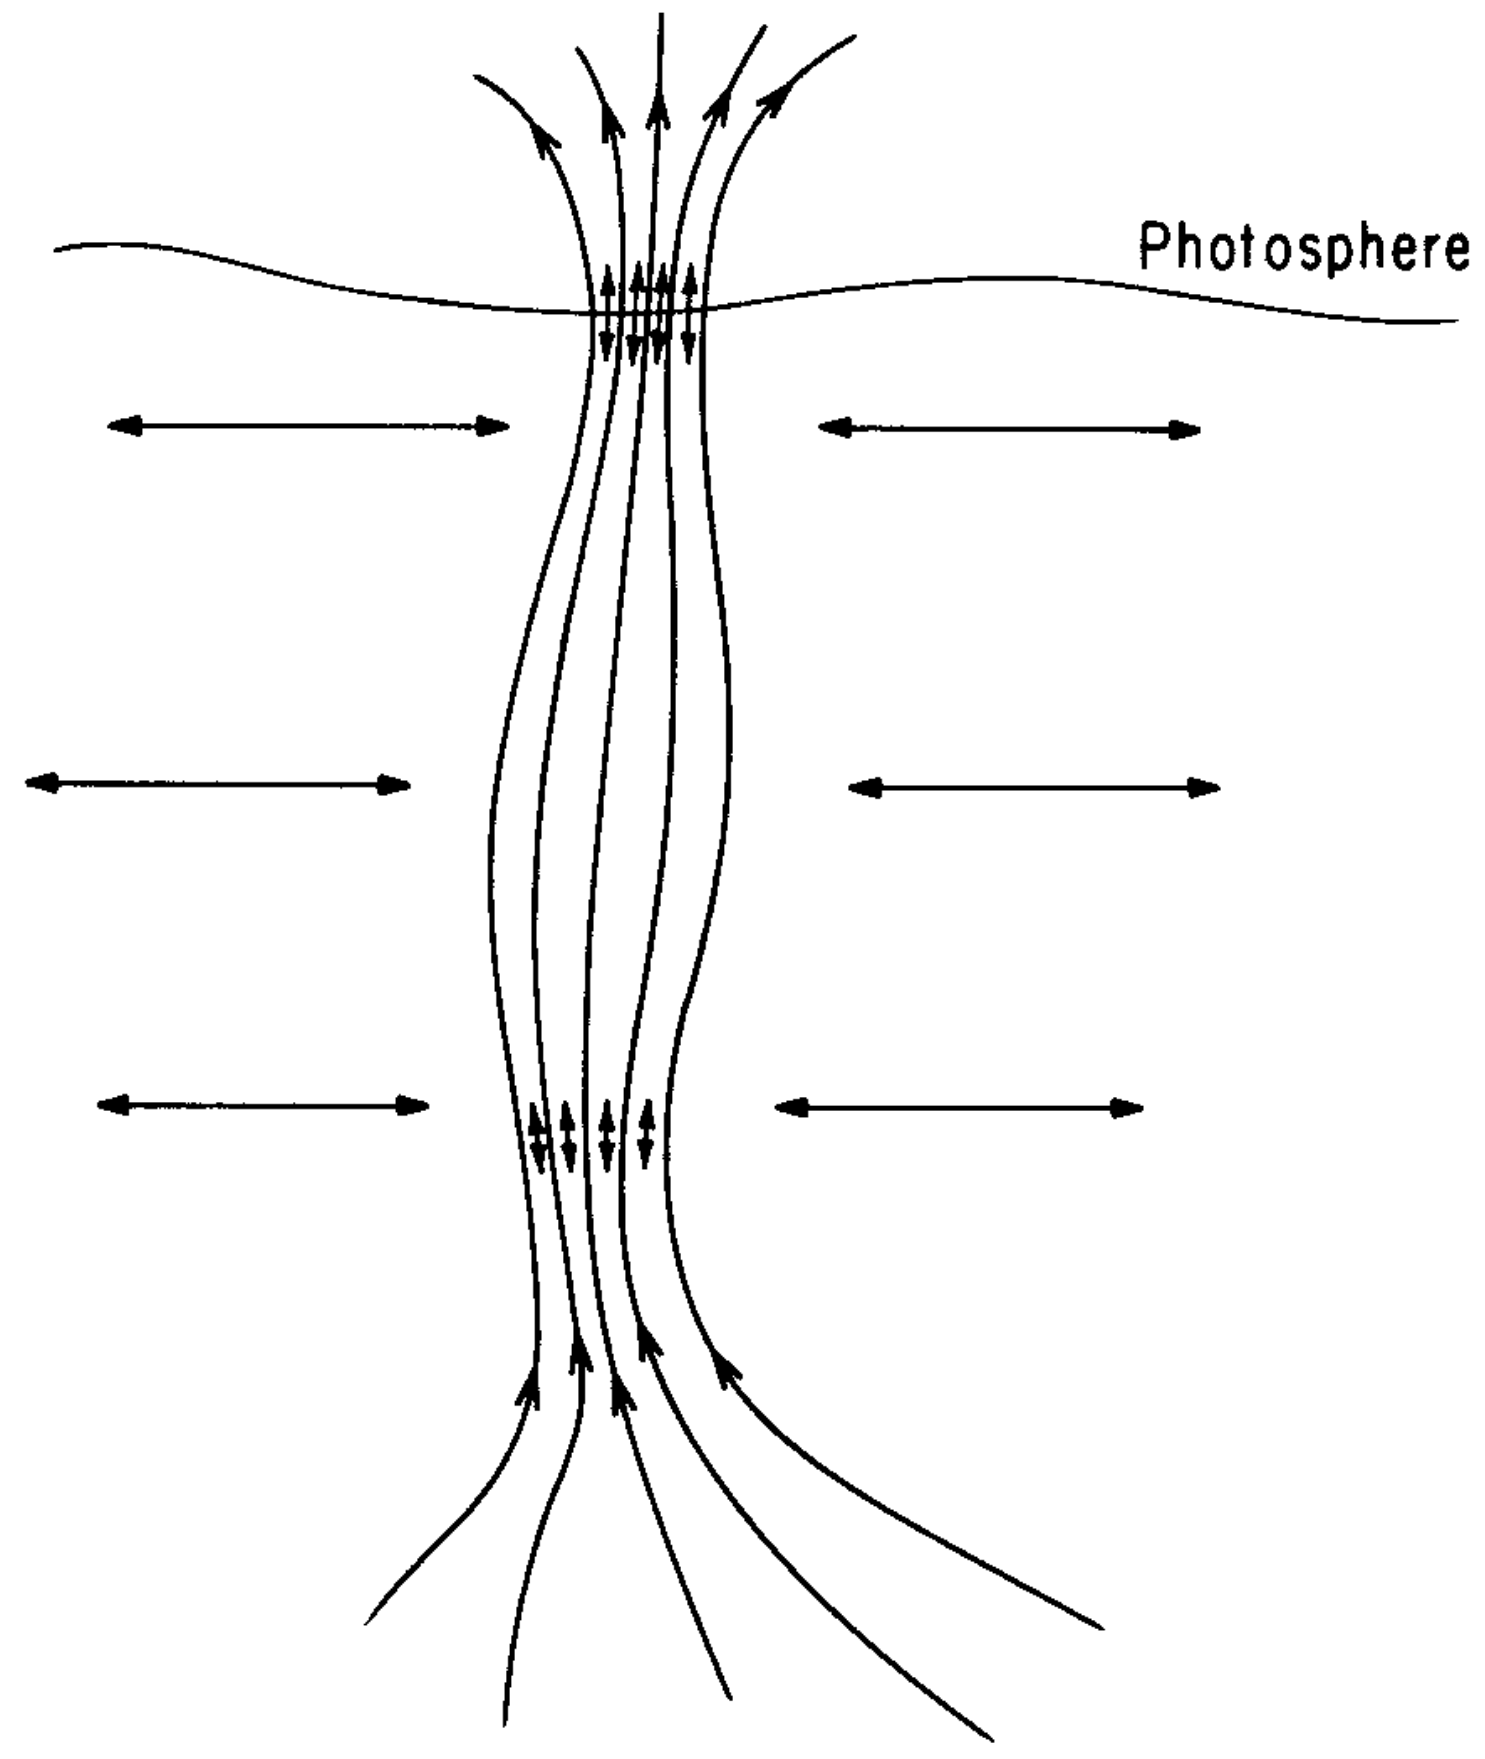
\includegraphics[align=t,width=\linewidth]{images/magnflux2.png}
\\[\jot]\flushleftright\color{mpcolor}\enquote{\emph{%
sketch of the magnetic lines of force in a magnetic filament extending up through the photosphere.}}\sourceatright{\cites{parker1974b}}%
}
Magnetic flux is a \emph{scalar} quantity, with SI dimension \furl{https://doi.org/10.1351/goldbook.M03684}{\textsf{magnetic flux}}, and measured in units of \furl{https://doi.org/10.1351/goldbook.W06666}{\emph{webers} (\unit{Wb})}.
This flux is usually calculated by means of a \emph{vector} quantity called \textsf{magnetic flux density}, measured in units of \furl{https://doi.org/10.1351/goldbook.T06283}{\emph{teslas} (\unit{T})}.

As we shall see in more detail in \chap\,\ref{cha:cons_magnetic}, magnetic flux differs from the other six main quantities in that it answers the two \enquote{how much?} questions \emph{in one lower dimension}: \enquote{How much magnetic flux crosses this surface?} and \enquote{How much magnetic flux crosses this line?}. It also requires a slightly different notion of orientation of a surface.

The \enquote{flux of magnetic flux} is therefore a flow connected to a line, and ordinarily called \textsf{electric potential difference} or \textsf{electric tension}, measured in units of \furl{https://doi.org/10.1351/goldbook.V06634}{\emph{volts} ($\unit{V} = \unit{Wb/s}$)}. This \enquote{flux of a flux} is usually calculated by means of a vector quantity called \textsf{electric field strength}, measured in units of \emph{volt per metre} (\unit{V/m}).

The magnetic flux density and the electric field strength together are usually called \enquote{electromagnetic field}, which is therefore commonly represented by vectors associated to each point in space. But it can also be interpreted and visualized as a collection of moving, oriented magnetic tubes or lines, either closed or extending indefinitely; somewhat analogously to how we visualize matter and charge, as moving blobs or points, but with one more dimension. This interpretation goes back to Faraday \parencites*{faraday1846}, Maxwell \parencites*{maxwell1855b}, and later Dirac \parencites*{dirac1955} among others, and today is conveniently used in some fields such as \furl{https://doi.org/10.1093/acrefore/9780190871994.013.21}{solar physics}, for example to study \furl{https://spaceplace.nasa.gov/solar-activity/}{sunspots} (see Ryutova \cites*{ryutova2015_r2018}).

\mynotew{To be completed in a later version}


\section{Energy}
\label{sec:intro_energy}

Energy is a \emph{scalar} quantity, with SI dimension \textsf{energy}, and measured in units of \emph{joules} (\unit{J}). Its flux is measured in  joules per second, also called \emph{watts} ($\unit{W}=\unit{J/s}$).

Equivalently we can speak of mass, with SI dimension \textsf{mass}, and measured in units of \furl{https://doi.org/10.1351/goldbook.K03391}{\emph{kilograms} (\unit{kg})}; its flux is measured in \emph{kilograms per second} (\unit{kg/s}).

\smallskip

%
\marginpar{\vspace{\baselineskip}\centering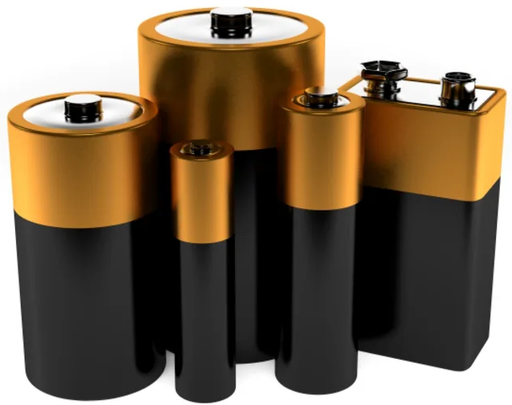
\includegraphics[width=\linewidth]{images/batteries.png}%
}%
The notion of energy is extremely important today, and central in many world-wide discussions and worries -- think of today's \enquote{energy crisis}, the need for \enquote{renewable energy}, and so on. It is somewhat funny that despite its importance it's actually difficult to answer \enquote*{what \emph{is} energy, really?}. Often we speak about energy as something that \enquote{flows}, is \enquote{transported}, \enquote{converted}, \enquote{stored}, and similar visualizations. This intuition will be enough in these notes. The notion of \emph{mass} is also very intuitive in our everyday life; we associate it with the \enquote{resistance} we feel when setting objects into motion, or with the weight of objects.
% relativity says that there's a strong connection between these two associations.

From Relativity Theory -- and experimentally -- we know that \emph{energy and mass are the same quantity}, and in these notes we shall emphasize this experimental fact.


\subsection{Energy and mass are the same}
\label{sec:mass_is_energy}

Let's see some examples of why it is impossible to make a distinction between energy and mass. The following examples have been simplified in some of their aspects, but their main point is valid.

\paragraph{Heated gas.}

Imagine we have a box with a given amount of gas, say \qty{1}{mol} of oxygen molecules. Using an extremely precise weighing scale, we observe that the mass of the gas is, say, exactly
\begin{equation*}
  \qty{0.031999540000000000}{kg} \ .
\end{equation*}
Now we heat the gas, providing \qty{60}{J} of energy, while making sure that not a single molecule of oxygen gets in or out of the box. The temperature of the gas increases by around \qty{3}{K}. We actually observe that the weight measured by the scale increases while we heat the gas, reaching the new value
% cp= 29.4 J/mol/K  cv=21.1
\begin{equation*}
  \qty{0.031999540000000668}{kg} \ .
\end{equation*}
Clearly the mass has increased, but no molecules were added! The additional mass is the \qty{60}{J} of energy that we provided to the gas by heating. Energy has weight, energy is mass.

% Some texts say that \enquote{mass is a form of energy}, but that's incorrect: mass \emph{is} energy, and energy in all its possible forms \emph{is} mass.

\paragraph{Stretched or moving rubber band.}

%
\marginpar{\vspace{\baselineskip}\centering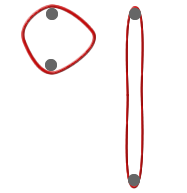
\includegraphics[width=\linewidth]{images/rubberbands.png}%
\\[\jot]\footnotesize\flushleftright\color{mpcolor}When we stretch a rubber band, its mass increases slightly -- even if the amount of rubber remains exactly the same.%
}%
Take a common rubber band, and imagine again that we have an extremely precise weighing scale. The rubber band, unstretched, has a mass of exactly
\begin{equation*}
  \qty{0.000500000000000000000}{kg}\ .
\end{equation*}
Now we stretch the band a little. By doing so we give energy to the band, which is said to acquire \enquote*{elastic energy}. Let's say we have given \qty{0.3}{J} to the band in this way.
% Refer later to elastic constant
% 0.5 * 50 N/m * (0.1 m)^2 \approx 0.3 J
Now we weigh the rubber band again, while stretched. We observe a mass of approximately
\begin{equation*}
  \qty{0.000500000000000003338}{kg} \ .
\end{equation*}
The extremely small difference of around \qty{3e-18}{kg} from the initial mass
is exactly the elastic energy that we provided by stretching.
Energy has weight; energy is mass.

\smallskip

Now set the unstretched band in motion. Owing to the motion, the band is said to have acquired \enquote*{kinetic energy}; let's say an amount \qty{0.3}{J}. If we could weigh the band while in motion (but without moving the weighing scale), we would observe again a mass of approximately
\begin{equation*}
  \qty{0.000500000000000003338}{kg} \ .
%\qty{0.000500000000000002225}{kg}
\end{equation*}
The small difference from the initial mass is the additional kinetic energy of the band. Energy has weight; energy is mass.

% This case is actually connected with the example of the gas above. If we observed the gas at a molecular level, we would interpret the energy of \qty{60}{J} provided to it as additional kinetic energy of its molecules. The increase in weight was exactly this additional kinetic energy.

\paragraph{Fission and atomic bombs.}
\marginpar{\vspace{-2\baselineskip}\centering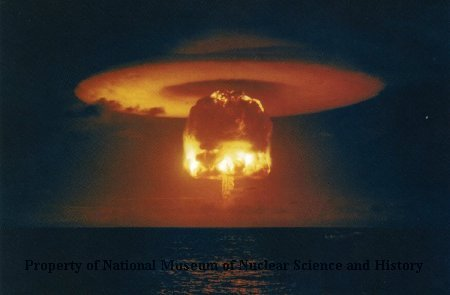
\includegraphics[width=\linewidth]{images/atomicbomb.jpg}%
\\[\jot]\flushleftright\color{mpcolor}\footnotesize\emph{Hydrogen Bomb Test, 1954%
}\\{(\furl{https://nuclearmuseum.pastperfectonline.com/Archive/716477C1-5E7A-485C-8BE1-857919471563}{National Museum of Nuclear Science \amp\ History})}%
}
%
The \furl{https://www.britannica.com/science/nuclear-fission}{atomic bomb} is a dark example of the fact that mass is energy. In phenomena of nuclear fission, we notice a decrease in the weight, measured at rest, of nuclear material before and after the phenomenon of fission. But we also observe that a great amount of (kinetic) energy is released. This amount is exactly equal to the apparently missing weight.

\paragraph{Electric heater.}

As a final example consider a \qty{1000}{W} electric heater, which is radiating \qty{1000}{J} in one second. The heater is also losing around \qty{0.00000000000001}{kg} of mass every second owing to this heat radiation -- although it's also acquiring the same amount of mass as electromagnetic energy.


\subsection{The practical use of the words \enquote*{mass} and \enquote*{energy}}
\label{sec:dist_mass_energy}

From the examples above it becomes clear that energy and mass are two names for the same thing.
%
\marginpar{\vspace{\baselineskip}%
\footnotesize\color{mpcolor}\enquote{\emph{%
we are led to the more general conclusion: The mass of a body is a measure of its energy content; if the energy changes by $L$, the mass changes in the same sense by $L/9\!\cdot\!10^{20}$, if the energy is measured in ergs and the mass in grams.
%\par Perhaps it will prove possible to test this theory using bodies whose energy content is variable to a high degree (e.g., salts of radium).
}}\sourceatright{\cites{einstein1905d}}%
}
%
The equivalence between energy and mass is given by the famous formula $E=m c^{2}$, where $c$ is the speed of light, \eqn~\eqref{eq:c}. In their respective units this gives
\begin{equation*}
  \begin{gathered}
    \qty{1}{kg} = \qty{89875517873681764}{J}\quad\text{(exactly)}
    \\
    \qty{1}{J} \approx \qty{0.0000000000000000111265}{kg}
  \end{gathered}
\end{equation*}
To grasp these numbers, consider that the mass of the rubber band in the example above, \qty{0.5}{g}, is comparable to the energy released by the \furl{https://www.britannica.com/story/atomic-bombing-of-hiroshima}{atomic bomb over Hiroshima}.

But it also becomes clear that in our daily experience we deal with energy-mass in two different ways:

On the one hand, we deal with huge (atom-bomb-like) amounts of energy packed in very small volumes: the huge amounts of energy that go together with objects like pens, keys, bicycles, cars, houses, and so on. We move, push, pull these huge energy amounts from one place to another, and even put them in our pockets. These energy amounts change a little all the time, as in the examples with the rubber band above. But these changes are so small as to be often undetectable with ordinary scales, and negligible for practical purposes. We call \enquote*{mass} any such huge amount of energy, and measure it with a unit -- \unit{kg} -- that doesn't lead to ridiculously large numbers. And we also agree to neglect the imprecision and fluctuation in its measurement, say any imprecision under \qty{0.000001}{\percent}. % This situation is similar to our measuring the power produced by power plants in megawatts (MW). We can say that another power plant constantly produces \qty{500}{MW}; but with this we don't really mean that it produces \emph{exactly} \qty{500000000.000}{W}: there are fluctuations all the time. And we can say that a power plant produces twice as much power, \qty{1000}{MW}, again with the understanding that the ratio is not \emph{exactly} \num{2.000000000000}.

On the other hand, we also deal with the small energy changes and exchanges in all these objects. These energy exchanges that are very important for our daily life: they keep us warm, keep our cells active, make our laptops work. In dealing with these energy exchanges, we don't care about the huge energy reservoirs they come from. So we agree to measure them with a unit -- \unit{J} -- that doesn't lead to ridiculously small numbers. And we also agree not to be precise about the total amount in the reservoir from which these energy bits come from.

As an analogy, think of when we speak about the amount of people in different countries. We can say that in Norway there are \num{5} millions, and in India \num{1500} millions, so in India there are \num{300} times more people. By this we don't mean that in Norway there are \emph{exactly} \num{5000000} people and that India has \emph{exactly} \num{300.000000} times more people. These numbers are changing slightly all the time, but we don't care about differences of 10 or even \num{10000} people. At the same time, if we have three dear friends or relatives visiting us from abroad, then the amount of \num{3} people is now for us very important. And we don't care about how large this amount is, compared to the total population of a country.

\smallskip

The distinction above is of course not clear-cut. In dealing with some physical phenomena, for example with few molecules or with subatomic particles, the fictitious but pragmatic distinction between mass and energy becomes too blurry and not useful anymore. In discussing these phenomena, indeed, one often uses the terms \enquote*{mass} and \enquote*{energy} interchangeably, as well as a common unit for both, such as the \furl{https://home.cern/tags/13-tev}{\emph{electronvolt}}.

\medskip

% From the examples above it is clear that the energy changes that we deal with and use in everyday situations are extremely small changes in mass -- so small that we can't measure them within the precision of ordinary weighing scales. Vice versa, the masses that we ordinarily deal with are huge amounts of energy. If we spoke only of \enquote*{energy} or only of \enquote*{mass} in all situations, and used only one unit, either joules or kilograms, we would have to work with very impractical numbers. \enquote*{Mass} can be considered a convenient term for \enquote*{energy} when huge amounts of it are involved, concentrated in small regions of space, and ordinary small energy changes can be neglected.
In these notes we shall often use the expressions \enquote*{\energym} and \enquote*{\masse} to remind ourselves that these two words denote the same physical thing.

\subsection{Different \enquote*{forms} of energy}
\label{sec:forms_energy}

We often speak of different \emph{forms} of \energym. The most important forms for us will be \textbf{internal energy}, \textbf{kinetic energy}, \textbf{gravitational potential energy}, to be discussed later. Another important one is \emph{electromagnetic energy}.

Later on we shall see that the differences among these energy forms come from the way they are calculated from other quantities, like matter or magnetic flux and electric charge. For example, if we know that in a volume there's an amount of a particular kind of matter, then we know that there must also be an amount of energy, given by a particular formula. And if that matter is moving, then we have to add to the energy an extra amount given by another formula. And if in that volume there's a gravitational field (that is, a particular kind of spacetime curvature), then another extra amount must be added, given by yet another formula. Similarly if we know that an electromagnetic field is in that volume.

We also speak of different forms of flux of energy. The most important for us will be \textbf{heat} and \textbf{mechanical power}. The difference is again in how these fluxes are calculated depending on whether there are also fluxes of matter and of other quantities.

\medskip

The distinctions between different forms of energy also depend on the observation scale and the theory used. For instance, we can observe and describe the water in a glass resting on table, on a scale of centimetres. We see it as a still, uniform fluid. In this description we say that the water has internal energy (or that there's internal energy in the glass). But if we observe and model that same water as a collection of molecules, on a microscopic scale, then we say that it has internal energy \emph{and} kinetic energy, because the molecules are in constant motion. The total amount of energy is the same on the centimetre-scale the  microscopic scale, but its partition into different \enquote{forms} depends on the scale.
%
\marginpar{\vspace{-5\baselineskip}\centering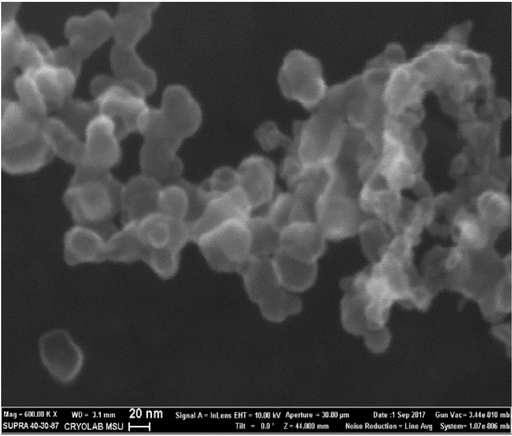
\includegraphics[width=\linewidth]{images/molecules_20nmb.png}%
\\[\jot]\footnotesize\flushleftright\color{mpcolor}\furl{https://doi.org/10.4209/aaqr.2019.04.0177}{Hydrocarbon fuel particles}. The small blobs have size of around \qty{2e-8}{m}.%
}%

The same is true of energy flux: what we call \enquote*{heat} on one observation scale, and appears as a flux of energy not associated with the motion of matter, may instead be called \enquote*{work} on a finer scale, and be associated with the motion of matter. % In phenomena that involve matter and electromagnetic fields, any separation between \enquote*{energy of matter} and \enquote*{energy of electromagnetic field} is often arbitrary.

% \begin{warning}[Amounts of \energym\ are coordinate-dependent]
%   Never change coordinate system in the middle of a calculation of energy change!
%   Although the distinction of energy forms is often useful, it's important to keep in mind that it is not absolute: \emph{it depends on the coordinate system, on the scale of observation, and on the theory used}.
% \end{warning}

% So whenever you hear about a distinction between forms of energy or energy fluxes, pay attentionwhich coordinate system and which observation scale are being used.

% Energy-mass is present wherever there's matter, charge, or magnetic flux, and vice versa. \emph{Its specific relation with these quantities depends on the coordinate system} (\sect\,\ref{sec:coords}) that we choose. It is extremely important to keep in mind this dependence. For instance, in the examples above we said that the unstretched rubber band in motion had a \masse\ of \qty{0.000500000000000002}{kg}; but if we choose a coordinate system in which the band is not moving, its \masse\ would be \qty{0.000500000000000000}{kg}. Owing to this coordinate dependence, and depending on whether matter or magnetic flux is present in a region, we often conveniently partition an amount of energy into different \enquote{forms} like rest energy, internal energy, kinetic energy, gravitational potential energy, electromagnetic energy. This is only a conceptual division.
%
% Also energy flux can be partitioned depending on the coordinate system and on whether there's also a flux of matter. This leads to the important distinction between two forms of energy flux: \textbf{heat} and \textbf{work}.
%
% We shall see later how to define and calculate these different forms of energy and energy flux.

\smallskip

\begin{definition}{Energy-mass: notation}
  The amount of energy in a volume is usually denoted with $\yE$, or with $\yM$ if we describe it as mass. % Internal energy is denoted $\yU$, kinetic energy $\yEk$, potential energy $\yEp$.
  The total flux of energy will be denoted by $\yH$.% ; the flux in the form of heat, by $\yQ$; and in the form of work, by $\yW$.
\end{definition}


\medskip

\begin{exercise}
  In an hour, 14 people exit through a door. Taking the average human weight to be \qty{62}{kg} \parencites{walpoleetal2012}, what's the average \emph{energy} flux, in \unit{J/s}, through that door?
\end{exercise}



% *** we shall see later in \sect

% electron: 8.2e-14 J
% 1e4 J intake
% 1 cal = 4 J
% 1 kg = 9e16 J
% U = 50/2*0.1^2 = 0.25 J = 3e-18 kg

\section{Momentum}
\label{sec:intro_momentum}

Momentum, also called \emph{linear momentum} or \emph{translational momentum} to distinguish it from angular momentum, is a \emph{vector} quantity. Its SI dimension and units can be written in several equivalent ways; we shall keep in mind especially these three:
\begin{equation*}
  \begin{gathered}
    \textsf{force}\times\textsf{time}
    \\\unit{N\cdot s}
  \end{gathered}
\enspace  \equiv\enspace
  \begin{gathered}
  \textsf{mass}\times\textsf{length}/\textsf{time}
    \\\unit{kg\cdot m/s}
  \end{gathered}
\enspace  \equiv\enspace
  \begin{gathered}
  \textsf{energy}\times\textsf{time}/\textsf{length}
    \\\unit{J\cdot s/m}
  \end{gathered}
\end{equation*}
% $\textsf{energy}\times\textsf{time}/\textsf{length}$, and accordingly measured in units of $\emph{joules}\times\emph{seconds}/\emph{metres}$ (\unit{J\cdot s/m}), or equivalently with SI dimension $\textsf{mass}\times\textsf{length}/\textsf{time}$, and accordingly measured in units of $\emph{kilograms}\times\emph{metres}/\emph{seconds}$ (\unit{kg\cdot m/s}).
Since it is a vector quantity, it is usually expressed with three numbers, typically the $x$-, $y$-, and $z$-components. In simplified problems where only one or two dimensions are relevant, only the relevant components are reported.
% \mynotew{use \unit{N\cdot s}}

Momentum is a subtle quantity, even subtler than energy. Textbooks that focus on Newtonian mechanics \emph{define} it as the product of the mass and the velocity of a body, usually written \enquote{$\bm{p}=m\bm{v}$}. This relation, however, is only valid in special circumstances, and cannot be used in many everyday technological applications, especially when electromagnetism is involved. And that relation is actually only an approximation even in the circumstances where it's used.

% First, it is true that where there's matter in motion there's also momentum; but this momentum is given by \enquote*{mass${}\times{}$velocity} only as an approximation. Second, there can be momentum also where there is no matter; for instance where there is magnetic flux. If you prepare a sealed glass box which is completely empty of matter within (you create a vacuum), there still is momentum within the box if light or electromagnetic waves are present. We shall discuss later some technological uses of this fact.

It is therefore convenient to separate our idea of momentum from the idea of \enquote{objects} moving, keeping in mind that the latter idea is just a particular case of momentum. Yet, \emph{momentum is indeed associated with translational motion} of matter and of electromagnetic fields. \emph{Translational} motion is the kind of motion that leads to a \emph{new position} in space. For instance, when you walk from one place to a different one, you have performed translational motion (note that translational motion doesn't need to be in a straight line).% We shall moreover see that there is an important connection between momentum and our intuitive idea of \enquote*{force}.

Just as energy can be mentally visualized as a sort of fluid (although this visualization comes with many warnings), also momentum can actually be visualized as a sort fluid; but you must imagine it as a \enquote{fluid of vectors}.
% \marginpar{%
% 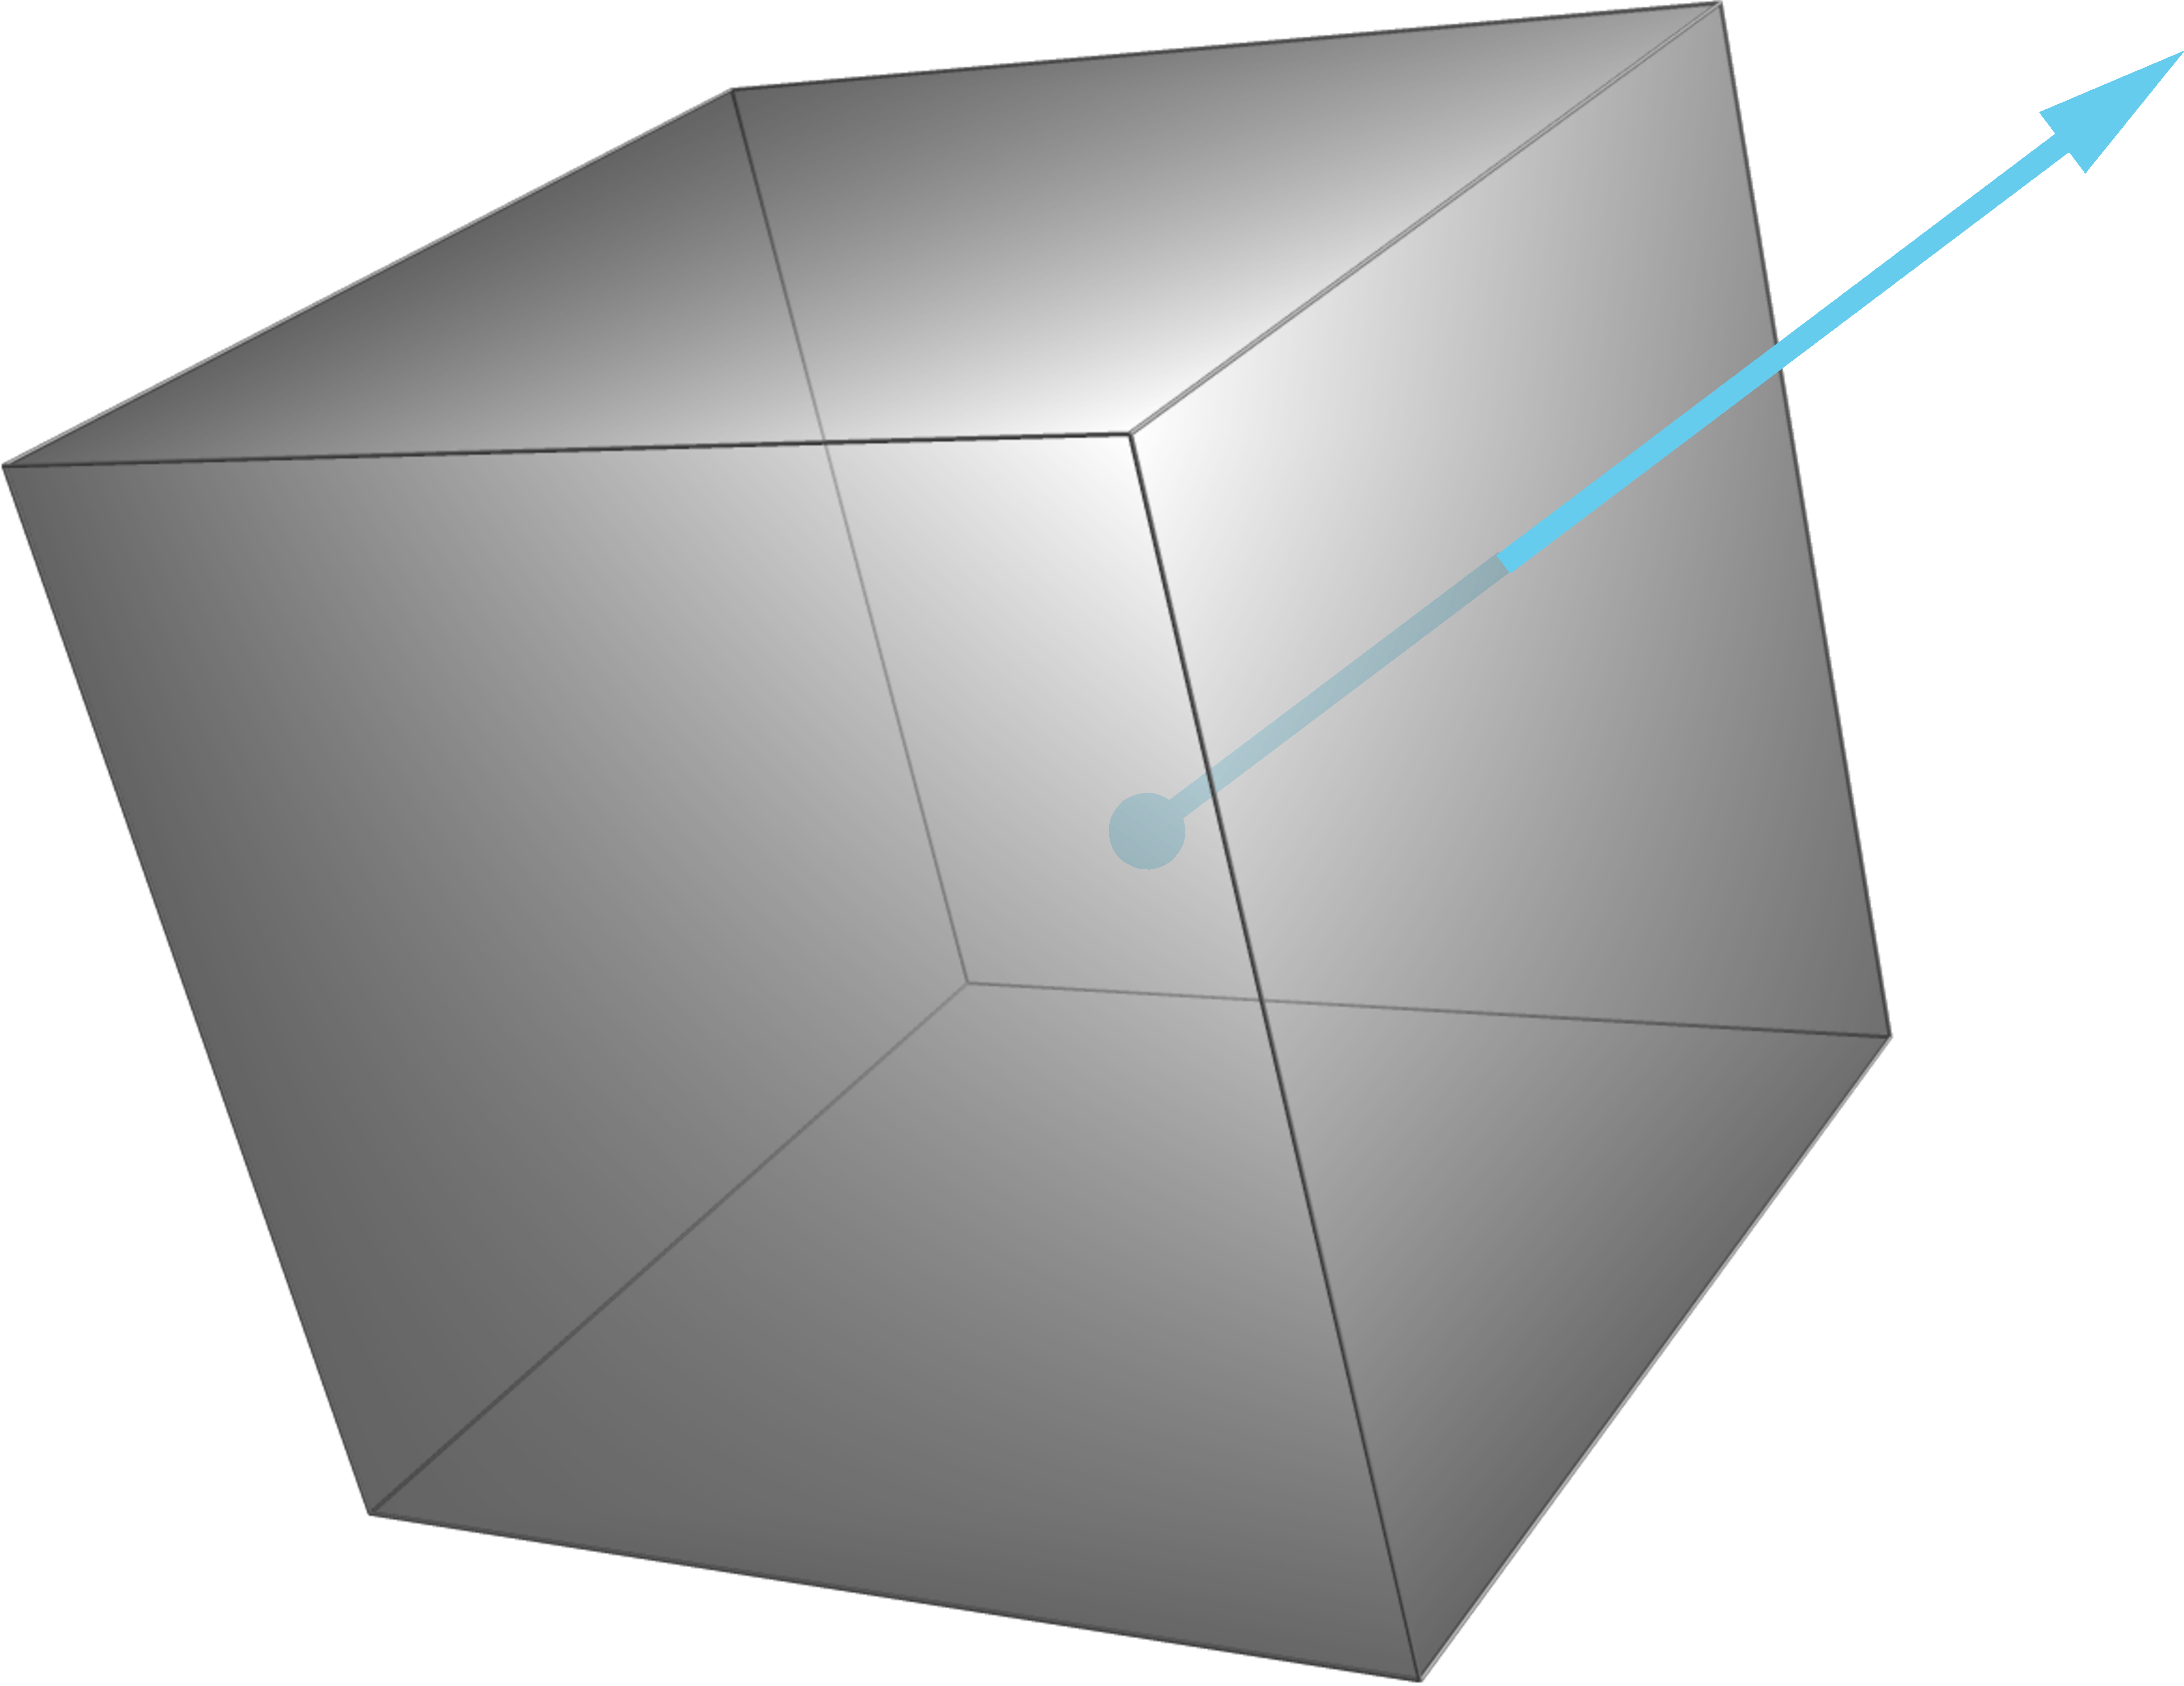
\includegraphics[align=t,width=\linewidth]{images/cubearrow.pdf}
% \\[\jot]\footnotesize\color{mpcolor}The amount of momentum within a volume is represented by a \textcolor{cyan}{(3D) vector}%
% }
%
\marginpar{\vspace{-3\baselineskip}\centering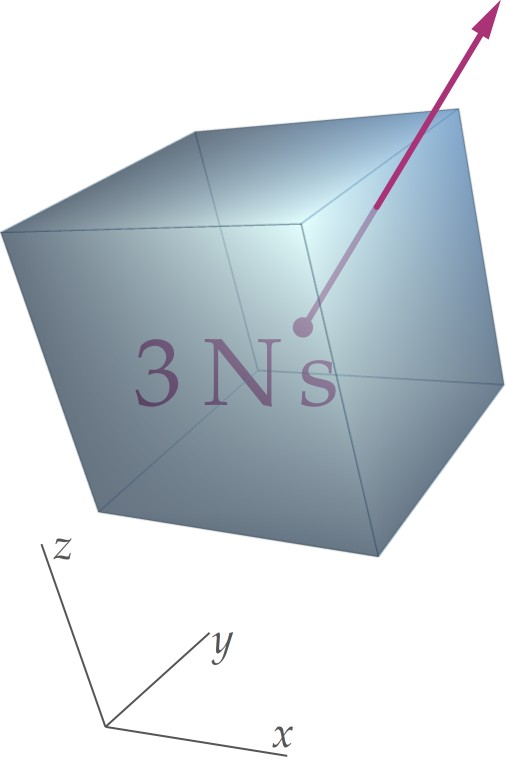
\includegraphics[align=t,width=\linewidth]{images/cube_Ns_coords.jpg}%
\\[\jot]\footnotesize\flushleftright\color{mpcolor}The amount of momentum within a volume at a given instant is represented by a \textcolor{purple}{3D vector}. The magnitude and direction of this vector depend on the coordinate system we're using.%
}%
Given a particular volume at a particular instant in time, and given a coordinate system, we can speak of the total amount of momentum within that volume. This amount is represented by a \emph{vector}. You can imagine a continuous collection of vectors filling the volume, possibly with different directions and small magnitudes; the total momentum is the sum of all these vectors. This visualization obviously comes with many warnings, but it can be very useful if we are careful.

\medskip

Flux of momentum is what we call \textbf{force}. A static force, like the one you exert when you hold a bag, is often mentally visualized as a static vector. In \chap\,\ref{cha:total_flux} we shall discuss a different visualization, in which force is represented as a sort of flow of vectors.

% Force is a notion that we understand intuitively and that we can \enquote{feel} with our own bodies. In Newtonian mechanics it's often taken as primitive, and is represented by a vector. But it can also be defined and interpreted as a \emph{flux of momentum}. This point of view can be very useful and even more intuitive in some situations. We shall discuss it more in depth in \sect\,\mynotew{}.


\begin{definition}{Momentum: notation}
  The amount of momentum in a region is usually denoted with $\yP$. The flux of momentum is also called force and denoted with $\yF$.
\end{definition}



\begin{extra}{Momentum and energy flux are the same}
  According to Relativity Theory, momentum \emph{is} energy flux (such as heat), and energy flux \emph{is} momentum. If we represent momentum with the symbol $\bm{P}$, and energy flux with the symbol $\bm{Q}$, the equivalence between them is given by
  \begin{equation}
    \label{eq:momentum_heat}
    \bm{Q} = \bm{P}c^{2}
  \end{equation}
  Compare this formula with $E=mc^{2}$. From this point of view, you can think of momentum as \enquote{energy in motion}. This is consistent with our discussion about \masse: since mass is energy, the Newtonian expression \enquote{$m\bm{v}$} indicates energy in motion, or a flux of energy. On a sunny day, if you close your eyes and feel the Sun's heat on your face, what you are feeling is actually a flow of momentum. And when you kick a ball, you're setting a huge bundle of energy in motion, and that's why the ball has acquired momentum.
\end{extra}



\section{Angular momentum}
\label{sec:intro_angmomentum}

Angular momentum, also called \emph{moment of momentum} or \emph{rotational momentum}, is a \emph{vector} quantity. Its SI dimension and units can be written in several equivalent ways; we shall keep in mind especially these three:
\begin{equation*}
  \begin{gathered}
    \textsf{force}\times\textsf{length}\times\textsf{time}
    \\\unit{N\cdot m\cdot s}
  \end{gathered}
\enspace  \equiv\enspace
  \begin{gathered}
  \textsf{mass}\times\textsf{length}^{2}/\textsf{time}
    \\\unit{kg\cdot m^{2}/s}
  \end{gathered}
\enspace  \equiv\enspace
  \begin{gathered}
  \textsf{energy}\times\textsf{time}
    \\\unit{J\cdot s}
  \end{gathered}
\end{equation*}
% , with SI dimension $\textsf{energy}\times\textsf{time}$, and accordingly measured in units of $\emph{joules}\times\emph{seconds}$ (\unit{J\cdot s}), or equivalently with SI dimension $\textsf{mass}\times\textsf{length}^{2}/\textsf{time}$, and accordingly measured in units of $\emph{kilograms}\times\emph{metres}^{2}/\emph{seconds}$ (\unit{kg\cdot m^2/s}).
It is usually expressed with three numbers, typically the $x$-, $y$-, and $z$-components.

Angular momentum is probably an even subtler quantity than momentum. Just as momentum is associated with translational motion, angular momentum is associated with \emph{rotational} motion. Rotational motion is the kind of motion that leads to a \emph{new orientation} in space, rather than to a new position. For instance, if you turn to your left or to your right while standing in place, you have performed rotational motion.

There isn't a clear-cut distinction between translational and rotational motion: usually they involve each other to some degree. A translational motion can be interpreted as a rotation around a point that is very far away; and a rotation of an extended object can be interpreted as small translational motions of its parts.

This is the reason why in many situations we can calculate angular momentum in terms of momentum. % so even if we don't fully grasp it intuitively, we can still calculate it
%
\marginpar{\vspace{-4\baselineskip}\centering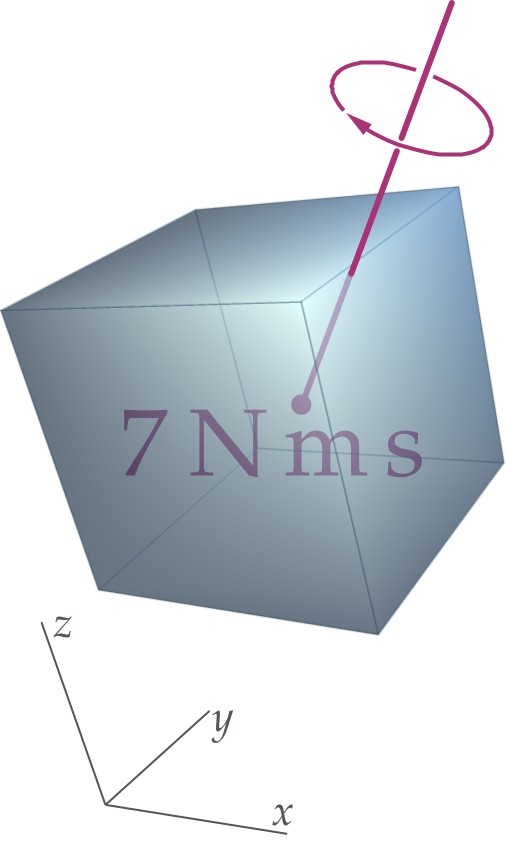
\includegraphics[align=t,width=\linewidth]{images/cube_Nms_coords.jpg}%
  \\[\jot]\footnotesize\flushleftright\color{mpcolor}The amount of angular momentum within a volume at a given instant is represented by a \textcolor{purple}{3D vector} (curious about the little circulation symbol around the vector? then read on). The magnitude and direction of this vector depend on the coordinate system we're using.%
}%
If the momentum in a \emph{small} volume is denoted by the vector $\yP=(P_{x},P_{y},P_{z})$, and the position vector by $\yr=(x,y,z)$, then the angular momentum $\yL=(L_{x}, L_{y}, L_{z})$ \emph{with respect to the origin of coordinates}, in that same volume, is given by the vector product
\begin{subequations}
  \begin{equation}
    \label{eq:ang_momentum_def}
    \begin{gathered}
      \yL = \yr \times \yP
      \\
      \text{or equivalently}\qquad\left\{\enspace
        \begin{aligned}
          L_{x} & = y\,P_{z} - z\,P_{y}
          \\    L_{y} & = z\,P_{x} - x\,P_{z}
          \\    L_{z} & = x\,P_{y} - y\,P_{x}
        \end{aligned}\right.
    \end{gathered}
  \end{equation}
  Instead of calling the components \enquote{$(L_{x}, L_{y}, L_{z})$}, we can also call them \enquote{$(L_{yz}, L_{zx}, L_{xy})$}, as some books do. The last names make the formulae above easier to remember:
  \begin{equation}
    \label{eq:ang_momentum_def_bis}
\left\{\enspace
    \begin{aligned}
      L_{yz} & = y\,P_{z} - z\,P_{y}
      \\    L_{zx} & = z\,P_{x} - x\,P_{z}
      \\    L_{xy} & = x\,P_{y} - y\,P_{x}
    \end{aligned}\right.
\end{equation}
\end{subequations}
Choose whichever you prefer.

Angular momentum is something that is associated not only with ordinary bodies (matter), but also with electromagnetic fields. Just like momentum, also angular momentum can be visualized as a \enquote{fluid of vectors}.
% %
% \marginpar{%
% 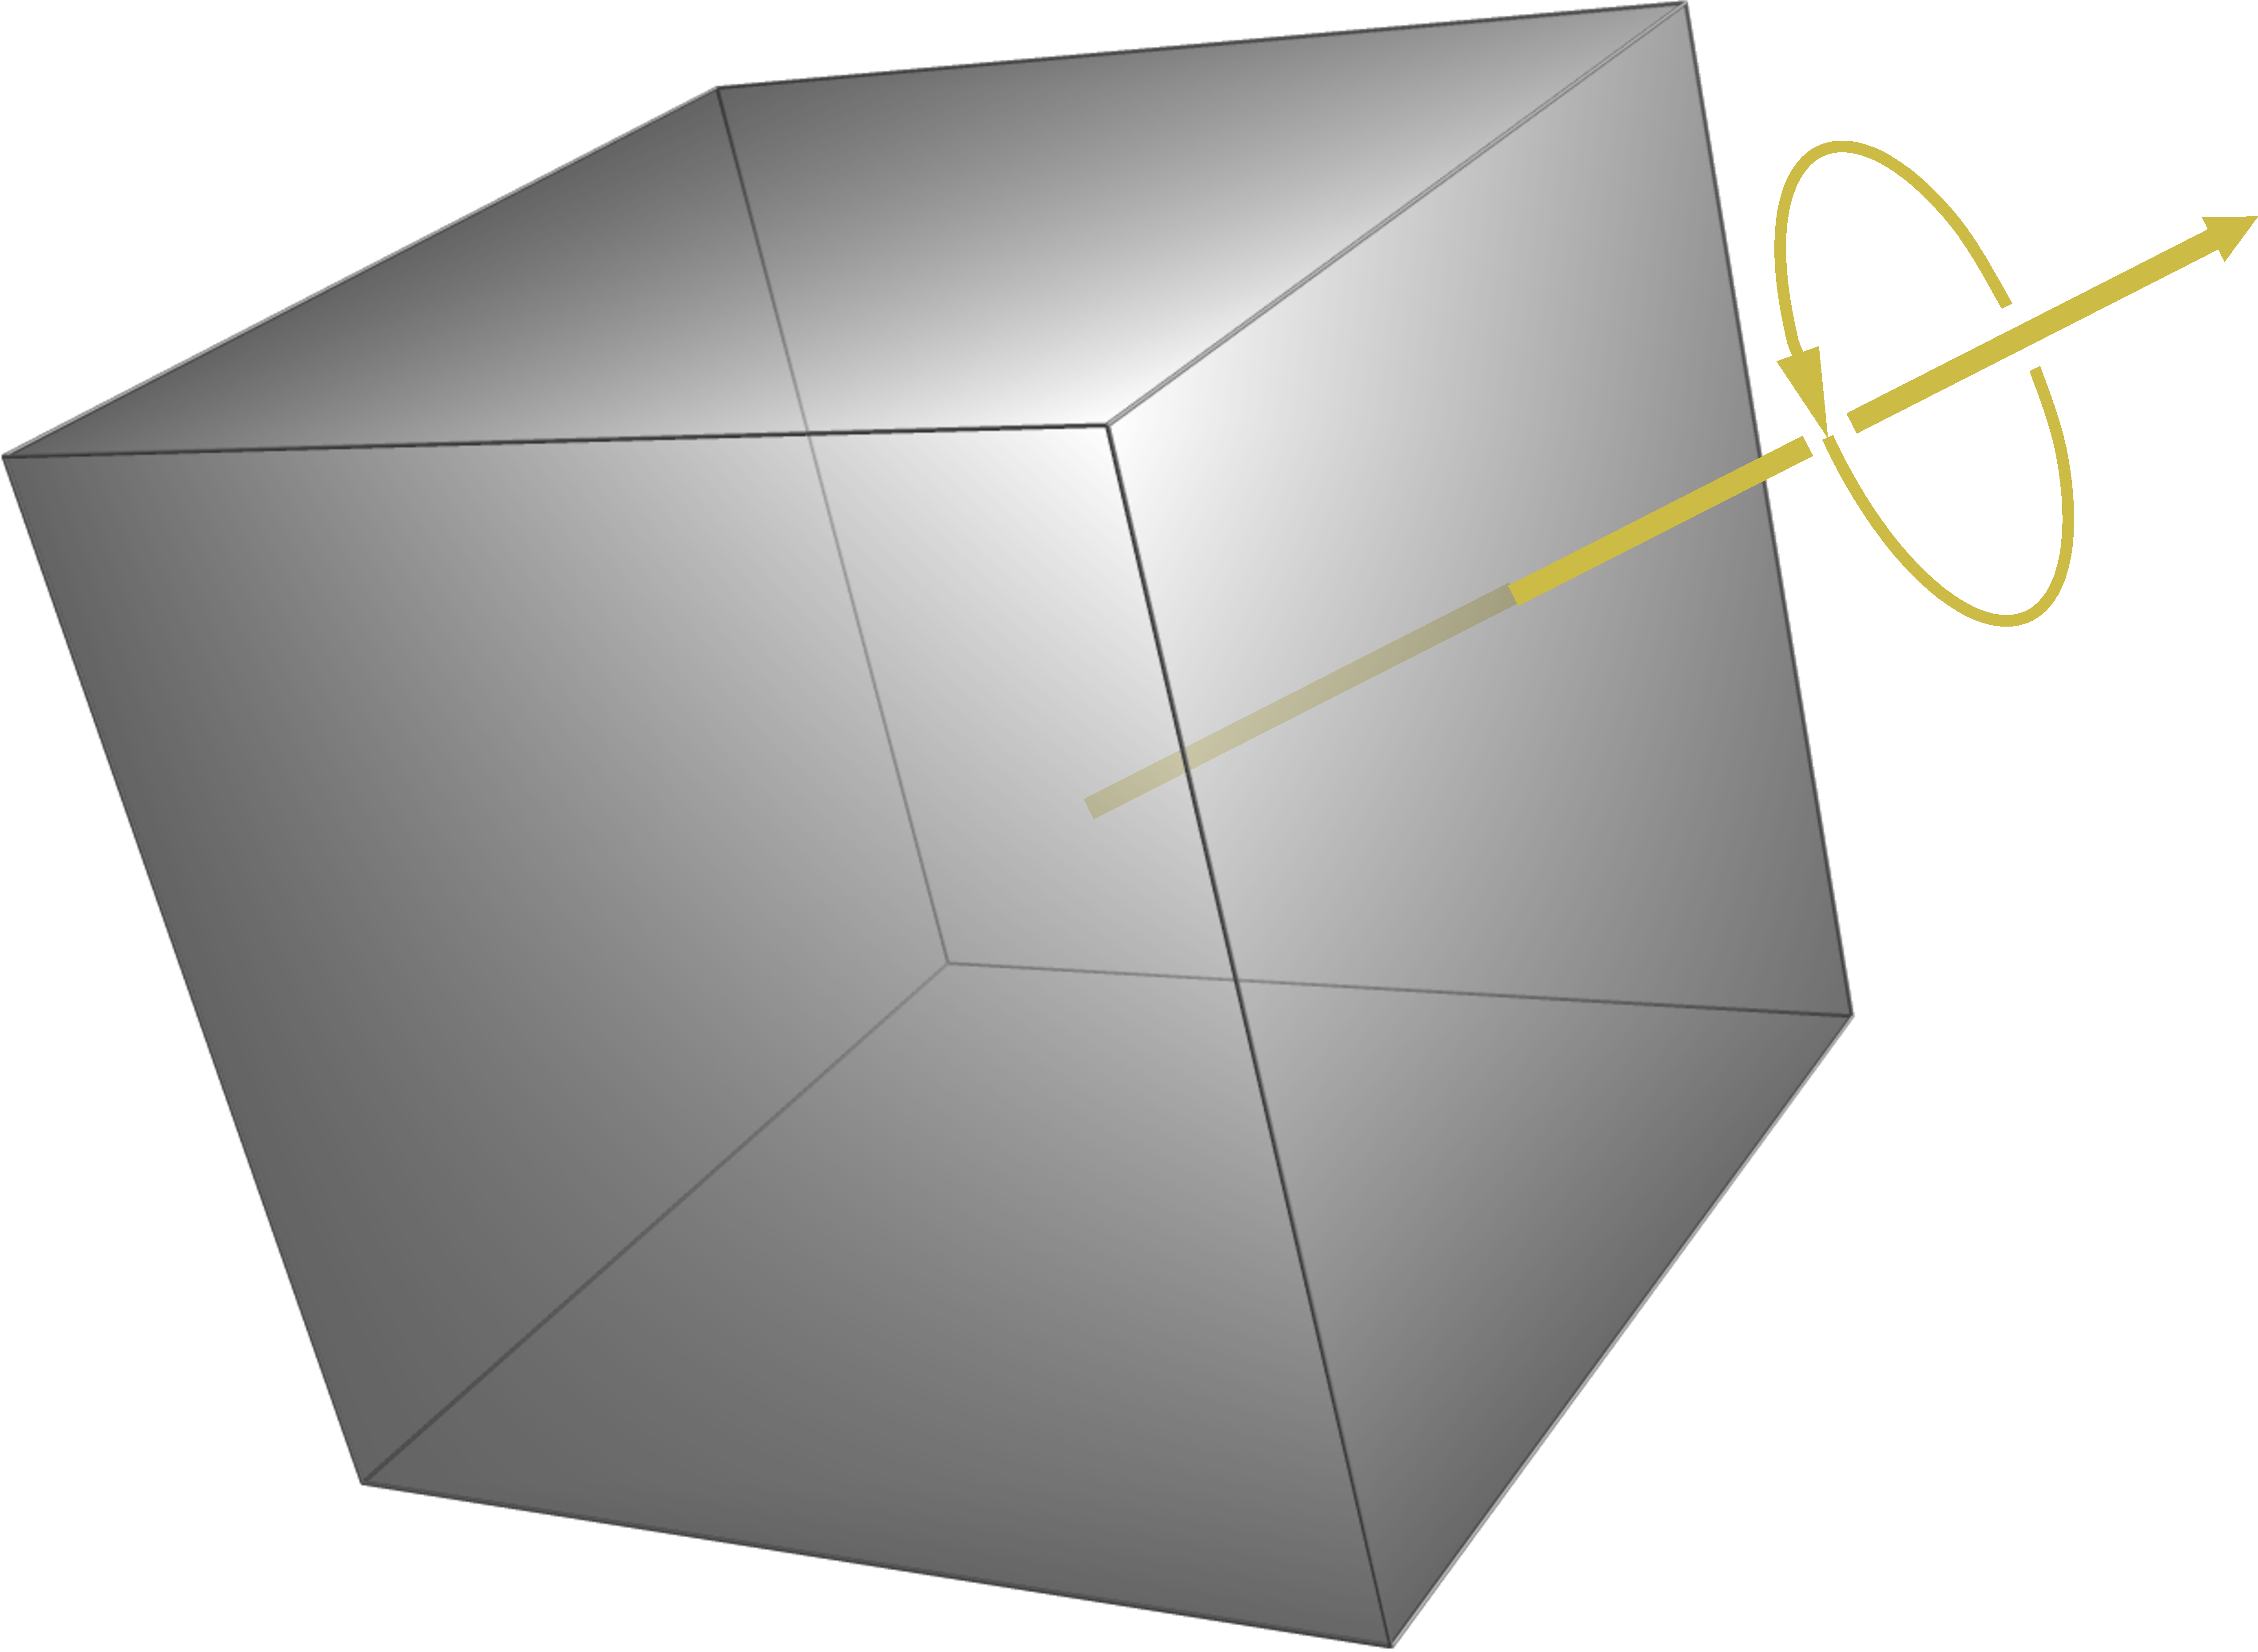
\includegraphics[align=t,width=\linewidth]{images/cubetwistedarrow.pdf}\label{fig:volumetwistedarrow}%
% \\[\jot]\footnotesize\color{mpcolor}The amount of angular momentum within a volume is represented by a \textcolor{yellow}{(3D) vector}. (Curious about the little circulation symbol around the vector? Then read on.)%
% }
Given a particular volume at a particular instant in time, and given a coordinate system, we can speak of the total amount of angular momentum within that volume. This amount is represented by a \emph{vector}.

\smallskip

The flux of angular momentum is also called the \emph{torque}, and bears a relation to the flux of momentum similar to the formula above. If the force -- flux of momentum -- is denoted by the vector $\yF=(F_{x},F_{y},F_{z})$ and the position vector by $\yr=(x,y,z)$, then the flux of angular momentum, or torque, $\yto=(\tau_{x}, \tau_{y}, \tau_{z})$ \emph{with respect to the origin of coordinates} is given by
  \begin{equation}
    \label{eq:torque_def}
    \begin{gathered}
      \yto = \yr \times \yF
      \\[\jot]
      \text{or equivalently}\qquad\left\{\enspace
        \begin{aligned}
          \tau_{x} & = y\,F_{z} - z\,F_{y}
          \\    \tau_{y} & = z\,F_{x} - x\,F_{z}
          \\    \tau_{z} & = x\,F_{y} - y\,F_{x}
        \end{aligned}\right.
      \qquad\text{or}\qquad
      \left\{\enspace
    \begin{aligned}
      \tau_{yz} & = y\,F_{z} - z\,F_{y}
      \\    \tau_{zx} & = z\,F_{x} - x\,F_{z}
      \\    \tau_{xy} & = x\,F_{y} - y\,F_{x}
    \end{aligned}\right.
    \end{gathered}
  \end{equation}

  \bigskip

\marginpar{\vspace{-3\baselineskip}\centering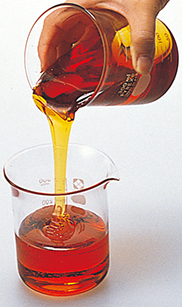
\includegraphics[width=0.67\linewidth]{images/polymer.png}%
\\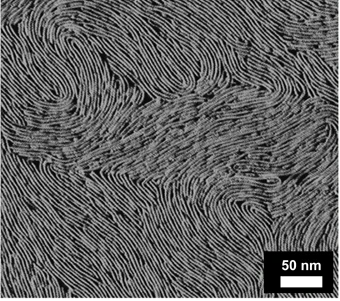
\includegraphics[width=\linewidth]{images/polymer2.png}%
\\[\jot]\flushleftright\footnotesize\color{mpcolor}Some liquid polymers (\textbf{top:} Liquid Diethoxymethane Polysulfide) need to be described with a special kind of angular momentum, owing to their molecular structure (\textbf{bottom}).%
}%
You may wonder:
\enquote{Do we really need angular momentum? after all it just looks like something constructed from momentum}.
The answer is yes, we really need it, for two reasons. First, angular momentum obeys an important universal law which is independent from those obeyed by energy and by momentum (\cites{truesdell1963b_r1968} tells some of the story of how this was discovered). % \mynotew{rephrase this}
Second, for some physical phenomena, for example involving liquid \furl{https://www.britannica.com/science/polymer}{polymers},
% https://www.britannica.com/science/polymer
elementary particles, or electromagnetic radiation, the angular momentum includes an additional part, called \emph{spin} or \emph{intrinsic angular momentum}, that is \emph{not} related to linear momentum. In the present notes we shall not use this more general kind of angular momentum.
% \begin{marginfigure}\footnotesize%
%   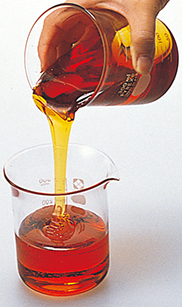
\includegraphics[align=b,width=\linewidth]{images/polymer.png}
% \\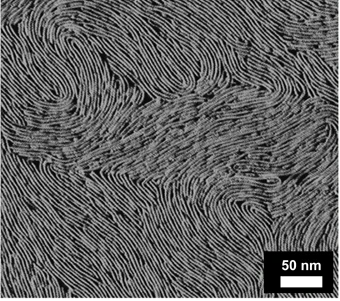
\includegraphics[align=c,width=\linewidth]{images/polymer2.png} \\[\jot]%
% {\color{green}Some liquid polymers (\textbf{top:} Liquid Diethoxymethane Polysulfide) need to be described with a special kind of angular momentum, owing to their molecular structure (\textbf{bottom}).}
% \end{marginfigure}

\smallskip

\begin{definition}{Angular momentum: notation}
  The amount of angular momentum in a region is usually denoted with $\yL$. The torque or flux of angular momentum is denoted with $\yto$.
\end{definition}




\begin{exercise}
  A GPS satellite has, at a given instant, the following position and momentum content:
  \begin{equation*}
    \begin{split}
      \yr &=\bigl[
      \num[exponent-mode=scientific]{1.4e+7}\,,\
      \num[exponent-mode=scientific]{1.6e+7}\,,\
      0\bigr]\:\unit{m}
      \\[\jot]
      \yP &=\bigl[
      \num[exponent-mode=scientific]{-3.1e+6}\,,\
      \num[exponent-mode=scientific]{3.4e+6}\,,\
      0\bigr]\:\unit{N\cdot s}
    \end{split}
  \end{equation*}
  Assuming that the satellite's volume can be considered small enough for the present purpose, calculate the satellite's angular momentum.
\end{exercise}



\subsection{Amounts of energy, momentum, angular momentum are coordinate-dependent}
\label{sec:energy_momentum_angmomentum_coords}


An aspect of energy, momentum, angular momentum that must always be kept in mind is that \textbf{their amounts depends on the coordinate system we're using}. If someone points at a specific region of space at a particular instant, and asks \enquote{how much energy is there?}, we \emph{cannot} give an answer until a coordinate system is specified. Once the coordinate system has been chosen, then a precise and unambiguous answer can be given. The same is true for the flow of energy through a surface, and for the amounts and fluxes of momentum and angular momentum. This also means that observers using different coordinates will usually assign different amounts of energy, momentum, angular momentum to the same regions of spacetime.

This is an important difference between energy, momentum, angular momentum on one side, and matter and electric charge on the other side. \emph{For matter and electric charge, the questions above can be answered unambiguously independently of any spatial coordinate system}.
%
\marginpar{\vspace{-5\baselineskip}\centering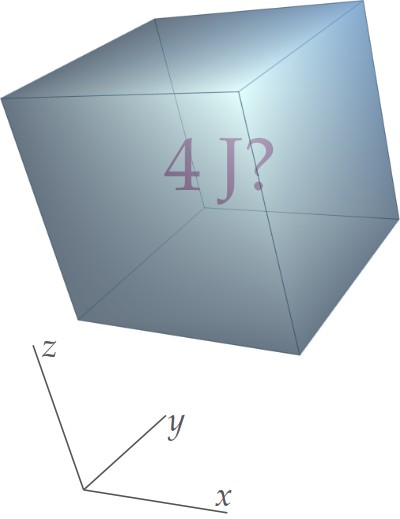
\includegraphics[align=t,width=\linewidth]{images/cube_J_coords.jpg}%
\\[\jot]\footnotesize\flushleftright\color{mpcolor}\enquote{How much energy is there in this volume at this instant?} -- This question cannot be answered until we have specified which coordinate system we're using.%
}

This coordinate-dependence is not a problem: we must always specify our coordinate system anyway, in order to agree on the time and position of physical events. But it can cause problems when we calculate \emph{changes} in energy. If we first calculate or measure some amount of energy in a coordinate system, then we calculate or measure another amount at some later time in a \emph{different} coordinate system, the difference between the two amounts has no meaning whatsoever. In fact it could happen that there's no energy change at all in one coordinate system or in the other: any change we found was just an artefact of mixing up coordinates.

\begin{warning}[{{Amounts of energy, momentum, angular momentum are coordinate-dependent}}]
  Never change coordinate system in the middle of calculations about energy, momentum, or angular momentum!
\end{warning}

% Also the distinction among different forms of energy is coordinate-dependent. For instance, in one coordinate system we can say that a given volume contains only internal energy; but in another coordinate system that same volume can be said to contain internal and kinetic energy.


\bigskip

\begin{extra}{{What are energy, momentum, angular momentum?}}
From the discussions and formulae above, it seems that \energym, momentum, angular momentum are quite closely related to one another. For all three, the amount in a volume or through a surface is undefined unless we specify a coordinate system. And we shall see later that all three satisfy balance laws but not necessarily conservation laws.

  Relativity Theory indeed shows that energy, momentum, angular momentum are different aspects of one single geometric object, called \emph{energy-momentum tensor}. They are like its \enquote{shadows}, that we can observe by looking at it from different points of view in time and space. This is also why their values get intermixed if we change our system of coordinates. %

  General Relativity gives a new meaning to these quantities: they are \emph{particular curvatures of spacetime}. They express how spacetime is curved in different directions. So whenever we measure, say, the energy or the momentum of some object or of some electromagnetic radiation, we are actually measuring how much that object or radiation is curving spacetime in a particular way. % We shall discuss further connections between these three quantities and spacetime in \sect\,\mynotew{}.
\end{extra}
\marginpar{\vspace{-11em}\centering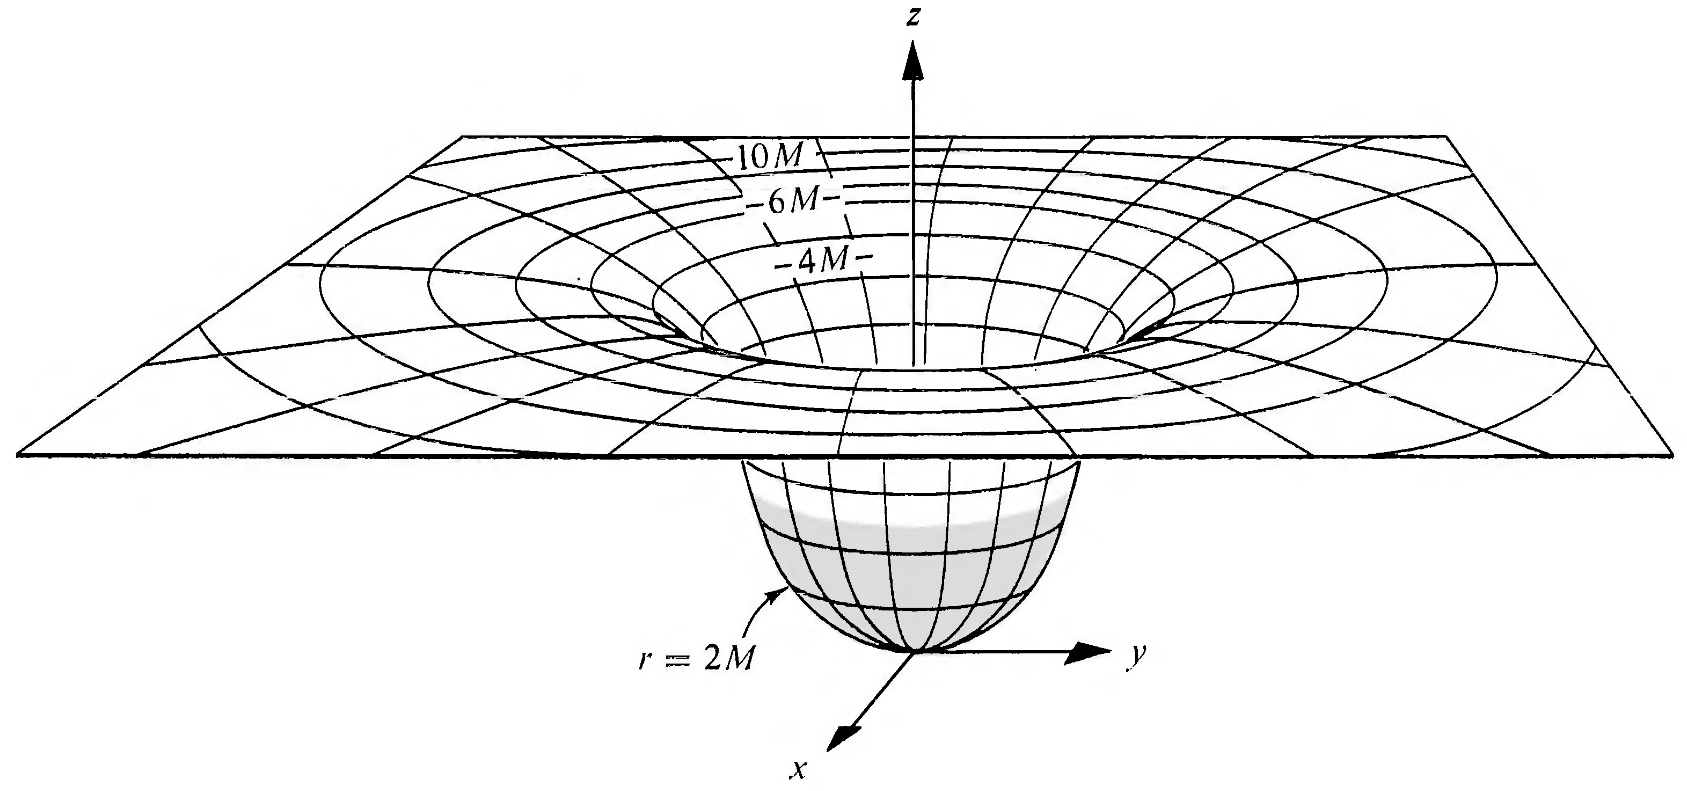
\includegraphics[width=\linewidth]{images/curvature1.png}%
\\[\jot]\footnotesize\flushleftright\color{mpcolor}Energy, momentum, angular momentum are measures of particular curvatures of spacetime.%
}%

\section{Entropy}
\label{sec:intro_entropy}

Entropy is a \emph{scalar} quantity, with SI dimension \textsf{energy$/$temperature}, and measured in units of \furl{https://doi.org/10.1351/goldbook.C01365}{\emph{joules}$/$\emph{kelvins} (\unit{J/K})}. From this definition it would seem that entropy is derived from temperature. However, although \textsf{temperature} is taken as primitive by the SI, the \furl{https://doi.org/10.1351/goldbook.K03374}{definition of temperature} actually depends on a fixed value of \furl{https://doi.org/10.1351/goldbook.B00695}{\emph{Boltzmann's constant}}, which has the dimension of \textsf{entropy}.

Entropy is probably the most difficult quantity to grasp intuitively. Many seemingly intuitive descriptions given in some textbooks are, unfortunately, unhelpful and even misleading.

One particularly misleading intuition is that entropy would be a \enquote{measure of disorder}. Besides the fact that \enquote{disorder} is very vague and subjective, it turns out that some physical phenomena, for example with \furl{https://www.britannica.com/science/liquid-crystal}{liquid crystals}, can be considered more \enquote{disordered}, and yet have \emph{lower} entropy, than others. See also the example in the side figure. We shall discuss more about such phenomena later on.
\marginpar{\vspace{-3\baselineskip}\centering%
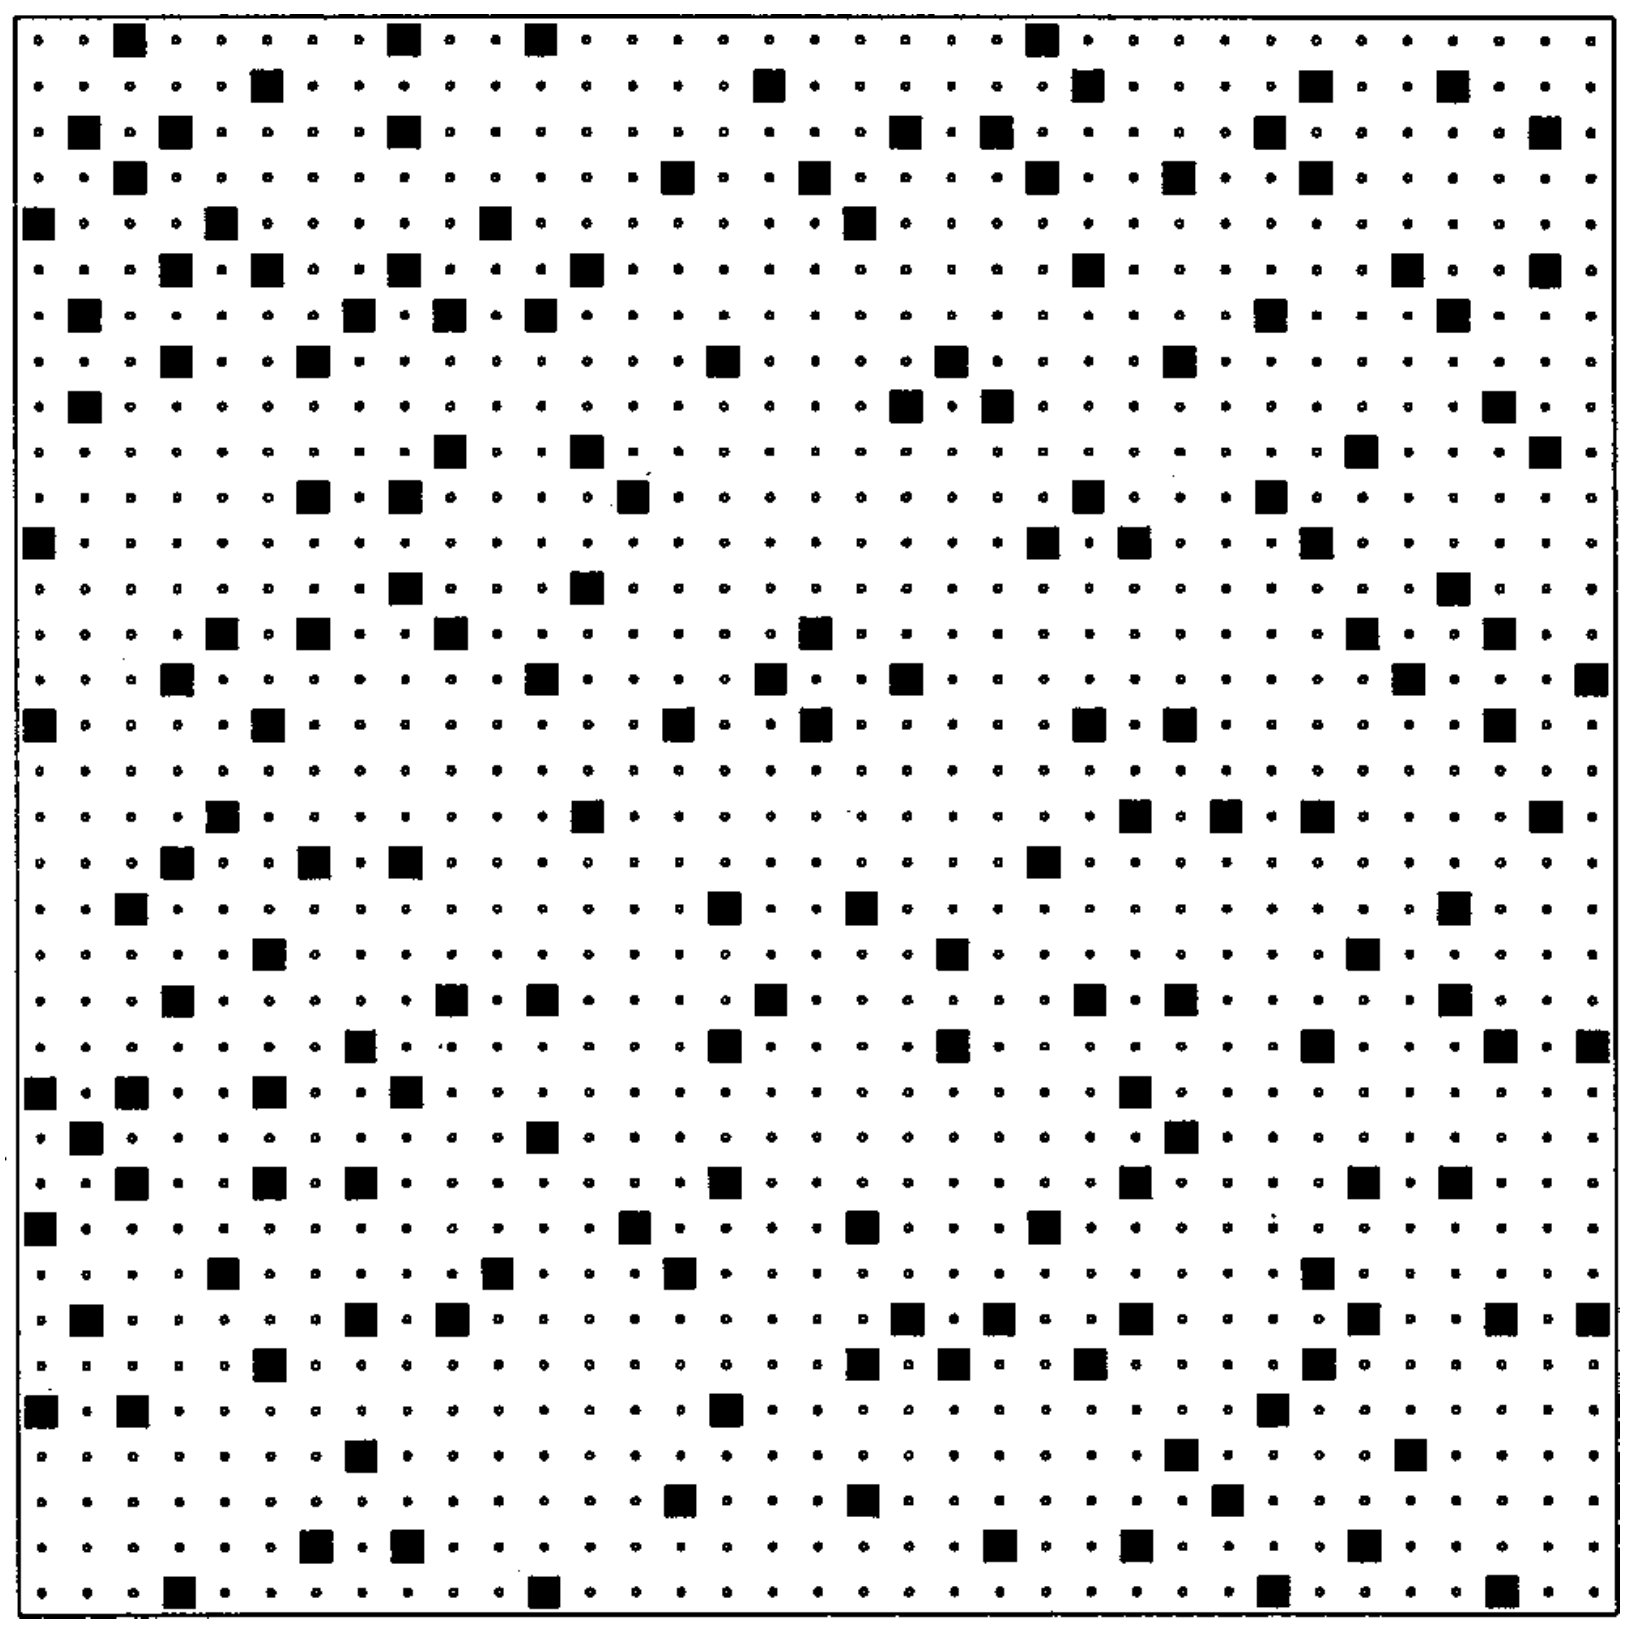
\includegraphics[width=\linewidth]{images/entropy_low.png}\\%
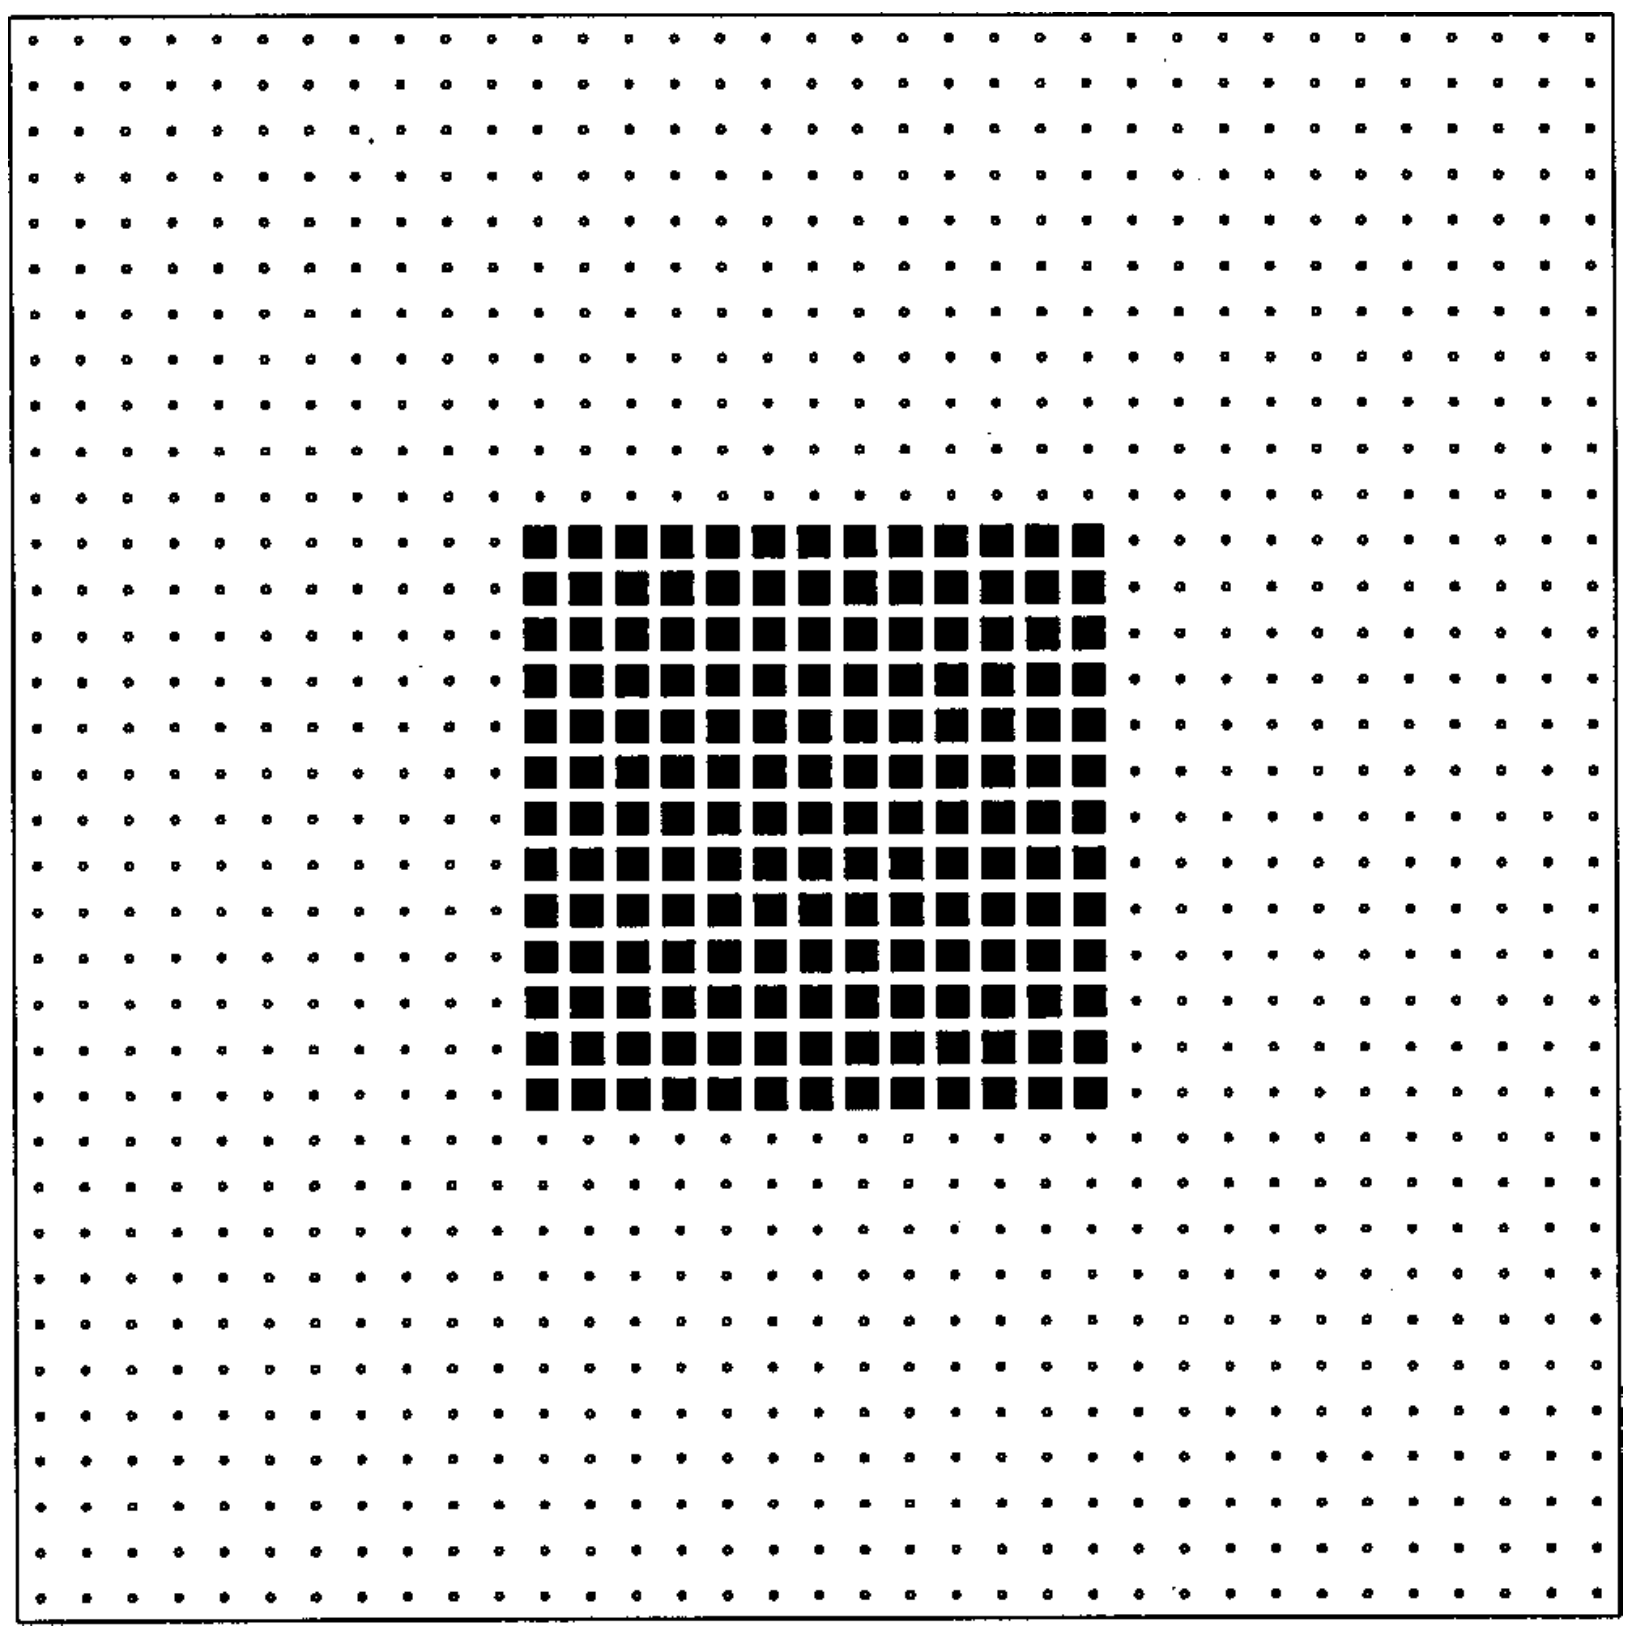
\includegraphics[width=\linewidth]{images/entropy_high.png}
\\[\jot]\flushleftright\footnotesize\color{mpcolor}Microscopic configurations of a lattice gas. \textbf{Left}: a configuration coming from a \emph{low}-entropy state. \textbf{Right}: a configuration coming from a \emph{high}-entropy state \parencites{styer2000}.%
}

In these notes we shall rely on the idea that \emph{entropy expresses a limit on the flux of energy into matter}. Said in simpler but more imprecise words, entropy is a bound on how fast we can heat up a body. We shall develop this idea further later.

One reason why entropy is difficult to grasp intuitively is that it has very different physical and mathematical aspects depending on the spatial scales and physical theory that we use to describe physical phenomena.

In many \enquote{continuum} phenomena, that is, phenomena where the molecular constitution of matter is not visible or not taken into account, entropy is treated as a \enquote{stuff-like} quantity similar to energy or electric charge. But there are difficulties also in this case. For some phenomena, for example involving non-elastic materials such as a simple paper clip, it is possible to introduce several entropies having different values -- and not just because of a change in measuring scale -- all of which can serve their purpose perfectly fine.

In molecular phenomena involving statistical mechanics, on the other hand, entropy is no longer a physical notion, but a \emph{probabilitistic} and \emph{statistical} one, related to guesses and inferences that we make about the physical phenomenon. Yet from many points of view it has roles similar to those of the entropy used in continuum phenomena.

We shall see later that the physical laws for entropy have also a different status with respect to the laws for the other six main quantities: they are, so to speak, \enquote{laws about laws}.

\smallskip

\begin{definition}{Entropy: notation}
  The amount of entropy in a region is usually denoted with $\yS$. We shall see that the flux of entropy is tightly related to heat, and we won't need a special symbol for it.
\end{definition}


\section{Auxiliary quantities}
\label{sec:aux_quantities}

Besides the seven principal quantities, other auxiliary quantities appear in some physical theories. Important examples are \textbf{temperature} and \textbf{strain}. Most auxiliary quantities are not extensive. For instance we cannot ask \enquote{what's the total amount of temperature in this region?}. We shall later discuss and use some auxiliary quantities, especially temperature.

The dimensions, units, and scalar or vector character of all quantities mentioned so far are summarized in table\,\ref{tab:units}.
\begin{table}
  \centering
  \begin{tabular}{lll}
    \hline\\
    \textbf{Quantity}&\textbf{SI Dimension}&\textbf{Unit}
    \\[2\jot]
    Time&\textsf{time}&\emph{second}\;\unit{s}
    \\[\jot]
    Length&\textsf{length}&\emph{metre}\;\unit{m}
    \\[\jot]
    Temperature&\textsf{temperature}&\emph{kelvin}\;\unit{K}
    \\[2\jot]
    Matter&\textsf{amount of substance}&\emph{mole}\;\unit{mol}
    \\[\jot]
    Electric charge&\textsf{electric charge}&\emph{coulomb}\;\unit{C}
    \\[\jot]
    Magnetic flux&\textsf{magnetic flux}&\emph{weber}\;\unit{Wb}
    \\[2\jot]
    Energy&\parbox[t]{10em}{\textsf{energy},\\[0\jot] \textsf{mass}}&\parbox[t]{5em}{\emph{joule}\;\unit{J},\\[0\jot] \emph{kilogram}\;\unit{kg}}
    \\[7\jot]
    \textbf{Momentum}
    &\parbox[t]{10em}{$\textsf{force}\cdot\textsf{time}$,
      \\[0\jot]$\textsf{mass}\cdot\textsf{length}/\textsf{time}$,
      \\[0\jot]$\textsf{energy}\cdot\textsf{time}/\textsf{length}$}
    &\parbox[t]{5em}{\unit{N\cdot s},
      \\[0\jot]\unit{kg\cdot m/s},
      \\[0\jot] \unit{J\cdot s/m}}
    \\[12\jot]
    \textbf{Angular momentum}
    &\parbox[t]{10em}{$\textsf{force}\cdot\textsf{length}\cdot\textsf{time}$,
      \\[0\jot]$\textsf{mass}\cdot\textsf{length}^{2}/\textsf{time}$,
      \\[0\jot]$\textsf{energy}\cdot\textsf{time}$}
    &\parbox[t]{5em}{\unit{N\cdot m\cdot s},
      \\[0\jot]\unit{kg\cdot m^2/s},
      \\[0\jot] \unit{J\cdot s}}
    \\[12\jot]
    Entropy&\textsf{energy$/$temperature}&\unit{J/K}
    \\[2\jot]
    \hline
  \end{tabular}
  \caption{Dimensions and units of the main physical quantities used in these notes. Their fluxes have the dimensions divided by time, and therefore units divided by seconds. Quantities in \textbf{boldface} are vectors, the others are scalars.}\label{tab:units}
\end{table}
% \begin{table}[tb]
%   \centering
%   \begin{tabular}{lll}
%     \hline\\
%     \textbf{Quantity}&\textbf{Geometric character}&\textbf{Unit}
%     \\[2\jot]
%     Time&\textsf{scalar}&\emph{second}\;\unit{s}
%     \\[\jot]
%     Length&\textsf{scalar}&\emph{metre}\;\unit{m}
%     \\[\jot]
%     Temperature&\textsf{scalar}&\emph{kelvin}\;\unit{K}
%     \\[2\jot]\color{green}
%     Matter&\color{green}\textsf{scalar}&\color{green}\emph{mole}\;\unit{mol}
%     \\[\jot]\color{purple}
%     Electric charge&\color{purple}\textsf{scalar}&\color{purple}\emph{coulomb}\;\unit{C}
%     \\[\jot]\color{red}
%     \textbf{Magnetic flux}&\color{red}\textsf{vector}&\color{red}\emph{weber}\;\unit{Wb}
%     \\[\jot]\color{blue}
%     Energy&\color{blue}\textsf{scalar}&\color{blue}\parbox[t]{5em}{\emph{joule}\;\unit{J},\\[0\jot] \emph{kilogram}\;\unit{kg}}
%     \\[5\jot]\color{cyan}
%     \textbf{Momentum}&\color{cyan}\textsf{vector}&\color{cyan}\parbox[t]{5em}{\unit{kg\cdot m/s},\\[0\jot] \unit{J\cdot s/m}}
%     \\[5\jot]\color{yellow}
%     \textbf{Angular momentum}&\color{yellow}\textsf{vector}&\color{yellow}\parbox[t]{5em}{\unit{kg\cdot m^2/s},\\[0\jot] \unit{J\cdot s}}
%     \\[5\jot]\color{midgrey}
%     Entropy&\color{midgrey}\textsf{scalar}&\color{midgrey}\unit{J/K}
%     \\[2\jot]
%     \hline
%   \end{tabular}
%   \caption{Dimensions and units of the main physical quantities used in these notes. Quantities in \textbf{boldface} are vectors, the others are scalars}\label{tab:units}
% \end{table}

\section{Metric}
\label{sec:metric}

A very important quantity constitutes an eighth fundamental building block of all our physical theories: the \textbf{metric}. It is quite different from the seven fundamental quantities, from both a physical and a geometrical point of view.

The metric characterizes our measurements of space and time. It's the object that allows us to calculate how much \emph{physical} time has elapsed, or the \emph{physical} distance between two objects, or the volume (say, in cubic metres) of a three-dimensional region of space, or the area (say, in square metres) of a surface. In General Relativity the metric allows us to calculate the curvature of spacetime.

The metric itself, in the technical sense of the so-called \enquote{metric tensor}, is \emph{not} an extensive quantity. We can't ask \enquote{what's the total amount of metric in this region?}; that would be a meaningless question. There are, however, other quantities which can be derived from the metric and which are extensive. Important examples are the so-called \enquote{volume density} and \enquote{area density}, which are the ones that allow us to calculate volumes and areas.

In the Newtonian approximation, that is, for speeds smaller than the speed of light and low energy densities (hence weak gravitational fields and small spacetime curvature), the metric is just a static, uniform background object, and spacetime has no curvature. This is why we can speak of an \enquote*{absolute time} and \enquote*{absolute distances} in this approximation. In these notes we shall for the most part use this Newtonian approximation.

In General Relativity the metric is a dynamic object instead: it can change in time, and can vary from one region space to another. These changes are determined by the seven fundamental quantities, and the metric, in turn, determines changes in the seven quantities.




\printpagenotes*
\clearpage
\chapter{Volume contents and fluxes}
\label{cha:total_flux}


\epigraph{For the sake of persons of these different types, scientific truth should be presented in different forms, and should be regarded as equally scientific, whether it appears in the robust form and the vivid colouring of a physical illustration, or in the tenuity and paleness of a symbolical expression.%
}{J. Clerk Maxwell \cites*{maxwell1870}}


Recall that the \autoref{cha:stuff}{main seven quantities} -- matter, electric charge, magnetic flux, energy, momentum, angular momentum, and entropy -- have three common properties related to their measurement:
\begin{enumerate}
\item[(1)] We can measure the amount of quantity within a three-dimensional region, at a specific time instant
\item[(2a)] We can measure the amount of quantity flowing through a two-dimensional surface during a time lapse\textellipsis
\item[(2b)] \textellipsis or alternatively we can measure the amount of quantity flowing through a two-dimensional surface \emph{per unit time}, at a particular time instant
\item[(3)]\label{item:extensivity}The amount in a volume consisting of separate volumes is equal to the total of the separate amounts. Similarly for the flux through separate surfaces.
\end{enumerate}

Let's give definite names to the measurements~(1) and~(2b):
\begin{definition}{volume content and flux}
  We can call measurement~(1) the \textbf{volume content} or \textbf{volume integral} of the quantity.

  \smallskip

  We call measurement~(2b) the \textbf{flux} of the quantity through the given surface.% Remember that in order to calculate the flux through a surface we need to specify how that surface is moving.
\end{definition}

\smallskip

These two notions and measurements are very intuitive. It is therefore convenient to base our physics upon them. In this chapter we straighten out some details about their definition and also about our intuition.

\section{Control volumes and control surfaces}
\label{sec:choice_surfaces}

For each of the main seven quantities we can therefore say how much of that quantity is in a given volume, or how much is flowing through a given surface. But how is this volume or surface chosen?

The choice of volume (and therefore of the surface bounding it) for a volume content, and the choice of surface for a flux are \emph{completely arbitrary}, and they can be \emph{imaginary}. Since they are under our control, and they allow us to control how the amounts of the seven quantities change, we call them \textbf{control volumes} and \textbf{control surfaces}.

For example, consider a classroom and the people in it. In your imagination you can divide the classroom into two halves, say the front and the rear half. You can then ask or measure simply by counting:\enspace
\begin{enumerate*}[label=(\arabic*)]
\item how many people are, right now, in the rear half;\enspace
\item how many people are crossing the imaginary division between the front and rear half during one minute, starting from now.
\end{enumerate*}

% The results of the two measurements above are numbers, which in general can be positive or negative, for scalar quantities; or vectors for vector quantities.
% % This number depends only on the chosen region, surfaces, and times.

\smallskip

A control volume and a control surface don't need to be static: they can move and deform:

In the case of a control volume, movement does not matter: the volume content in a control volume \emph{does not depend on the instantaneous motion of the volume}. In fact we can even imagine a control volume that exists for just one time instant.

% 
\marginpar{\vspace{-4\baselineskip}\centering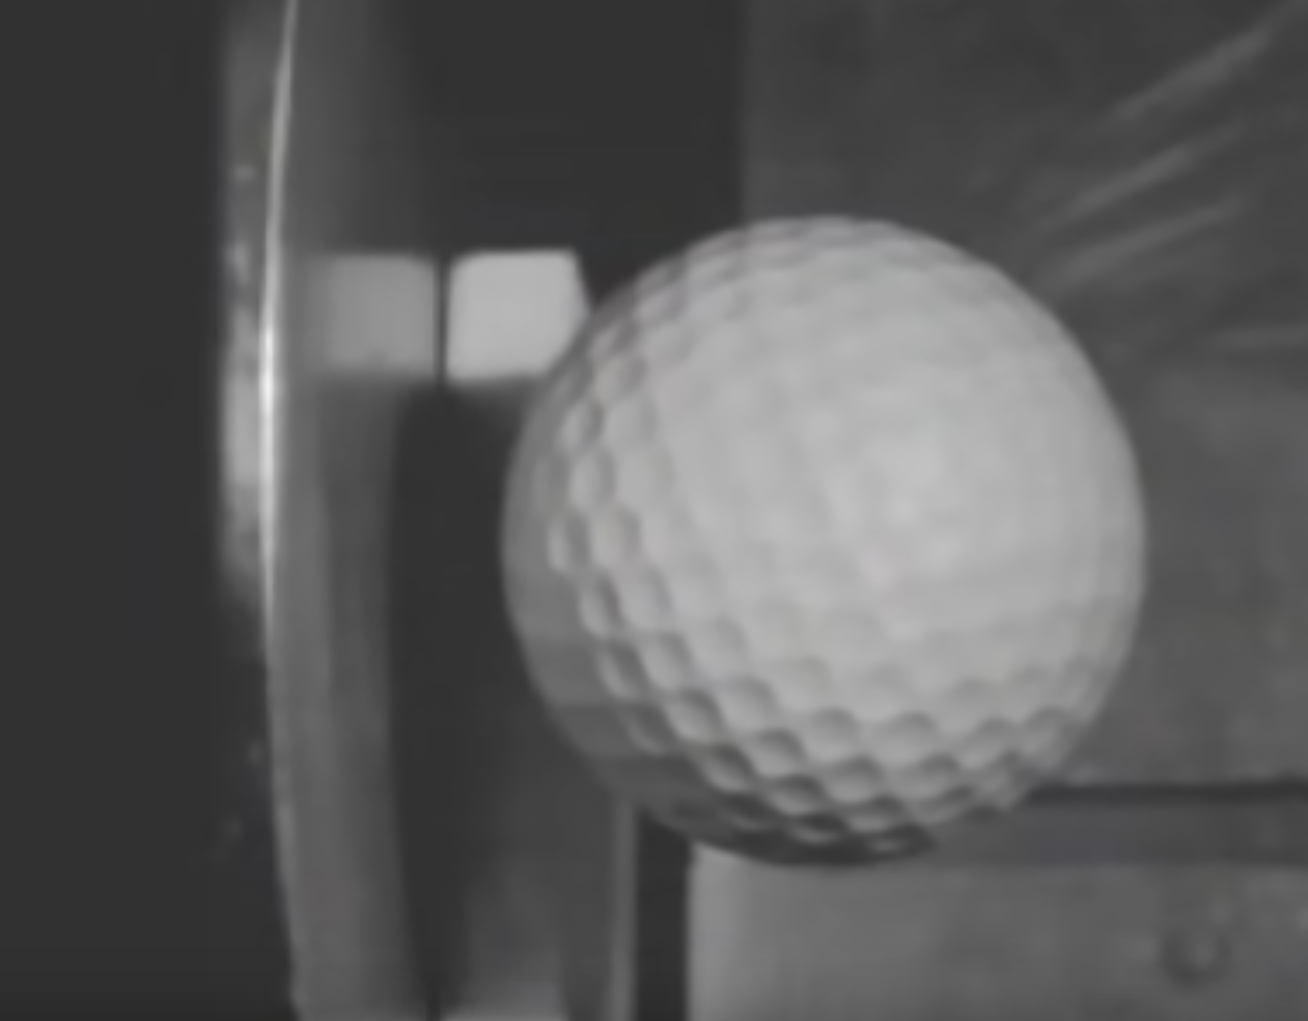
\includegraphics[width=\linewidth]{images/ball_wall.png}%
\\[\jot]\footnotesize\flushleftright\color{mpcolor}The golf ball is moving leftwards. Will it hit the metal surface? We don't know unless we know how the surface is moving.%
}%
In the case of a control surface the situation is different. The flux through a control surface \emph{depends also on the motion of the surface}. As a trivial example, consider a glass surface, and a person on one side of it, moving with a high velocity directed towards the surface. Will the person crash on the glass? We can't say for sure. The glass surface could be a glass wall in a building, which is not moving with respect to the person. In this case the person will likely crash on it. Or the glass surface could be the windscreen of a car, and the person could be the car's driver. In this case the person won't crash on the glass surface, because they're moving together with the same motion. Therefore we can't just imagine a surface that exists for one time instant: we need to imagine it at least for a very short time lapse, and be able to say how it's moving. If someone asks us what's the flux through a control surface at a given instant, but we are not told what's the motion of the surface, then the flux is unknown.


\begin{definition}{Control volume}
  A \textbf{control volume} is an arbitrary three-dimensional region of space at a given (coordinate) time. This region can have any position, shape, and size; it can even consist of several disconnected three-dimensional regions. This region does not need to exist before or after the given time.

  \smallskip

  We can also consider a \emph{temporal sequence} of control volumes, one for each instant of time. They can have positions, shapes, sizes that change smoothly from one time instant to the next. This sequence is often also called \enquote*{control volume} for short (but note the difference from the original meaning, which refers to only one time instant).
\end{definition}
\begin{definition}{Control surface}
  A \textbf{control surface} is an arbitrary two-dimensional region of space at a given (coordinate) time. This region can have any position, shape, and size; it can even consist of several disconnected two-dimensional regions.

  \smallskip

  The instantaneous movement and velocity of such a region is important; therefore this region must, intuitively speaking, exist also an instant right before and right after the given time.

  \smallskip

  We can also consider a \emph{temporal sequence} of control surfaces, one for each instant of time. They can have positions, shapes, sizes that change smoothly from one time instant to the next. This sequence is often also called \enquote*{control surface} for short (but note the difference from the original meaning, which refers to only one time instant).
\end{definition}


The fact that we can choose control volumes and control surfaces arbitrarily gives us a lot of power in solving physics problems and in making predictions. Typically they are chosen so as to simplify the equations that describe the physical situation, to simulate physical phenomena in a more precise way, and to focus on details of interest.
%
\marginpar{\vspace{-3\baselineskip}\centering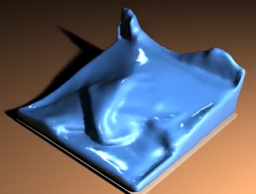
\includegraphics[width=\linewidth]{images/liquidvolume.png}%
\\[\jot]\footnotesize\flushleftright\color{mpcolor}Clever choice of control volumes and surfaces allow us to model and predict complex motions of fluids; \furl{http://www.youtube.com/watch?v=M5xnAdVPbgQ}{see also animation} (\cites{wojtanetal2009})%
}%

When we study some solid object, like a football, a rocket, or a planet, we typically choose a control volume that tightly encloses the object. When we study something flowing or moving, like a fluid material or an electromagnetic field, we typically divide the space of interest into small control volumes and surfaces, constructing a \emph{mesh}; this mesh can even be refined in regions that are of special interest.

\section{Volume content}
\label{sec:intuition_volume}

\subsection{Scalar quantities}

A volume content (or volume integral) for a scalar quantity, for example energy, can be represented like this:
\begin{center}
  
\includegraphics[align=t,height=7em]{images/volumeintegral_8J.pdf}
\end{center}
we have eliminated one spatial dimension for simplicity, considering the analogous two-dimensional idea. The volume is in \textcolor{midgrey}{light grey}, delimited by a closed \textcolor{darkgrey}{darker grey} boundary, and we're indicating that the volume content, that is, the amount of energy within, is \textcolor{blue}{\qty{8}{J}}.

As a visualization device, this representation can be useful. But let's straighten out some of its aspects:
\begin{itemize}[para]
\item Recall that this is a snapshot at a given time instant. So there are \qty{8}{J} of energy in the volume at that instant, but we don't know the situation earlier or later: there could be a different amount of energy, the region might be at a different position and have a different shape, or it might not even exist.

\item Recall that some scalar quantities, like electric charge and in some situations matter (antimatter), can have negative amounts.
\marginpar{\centering%
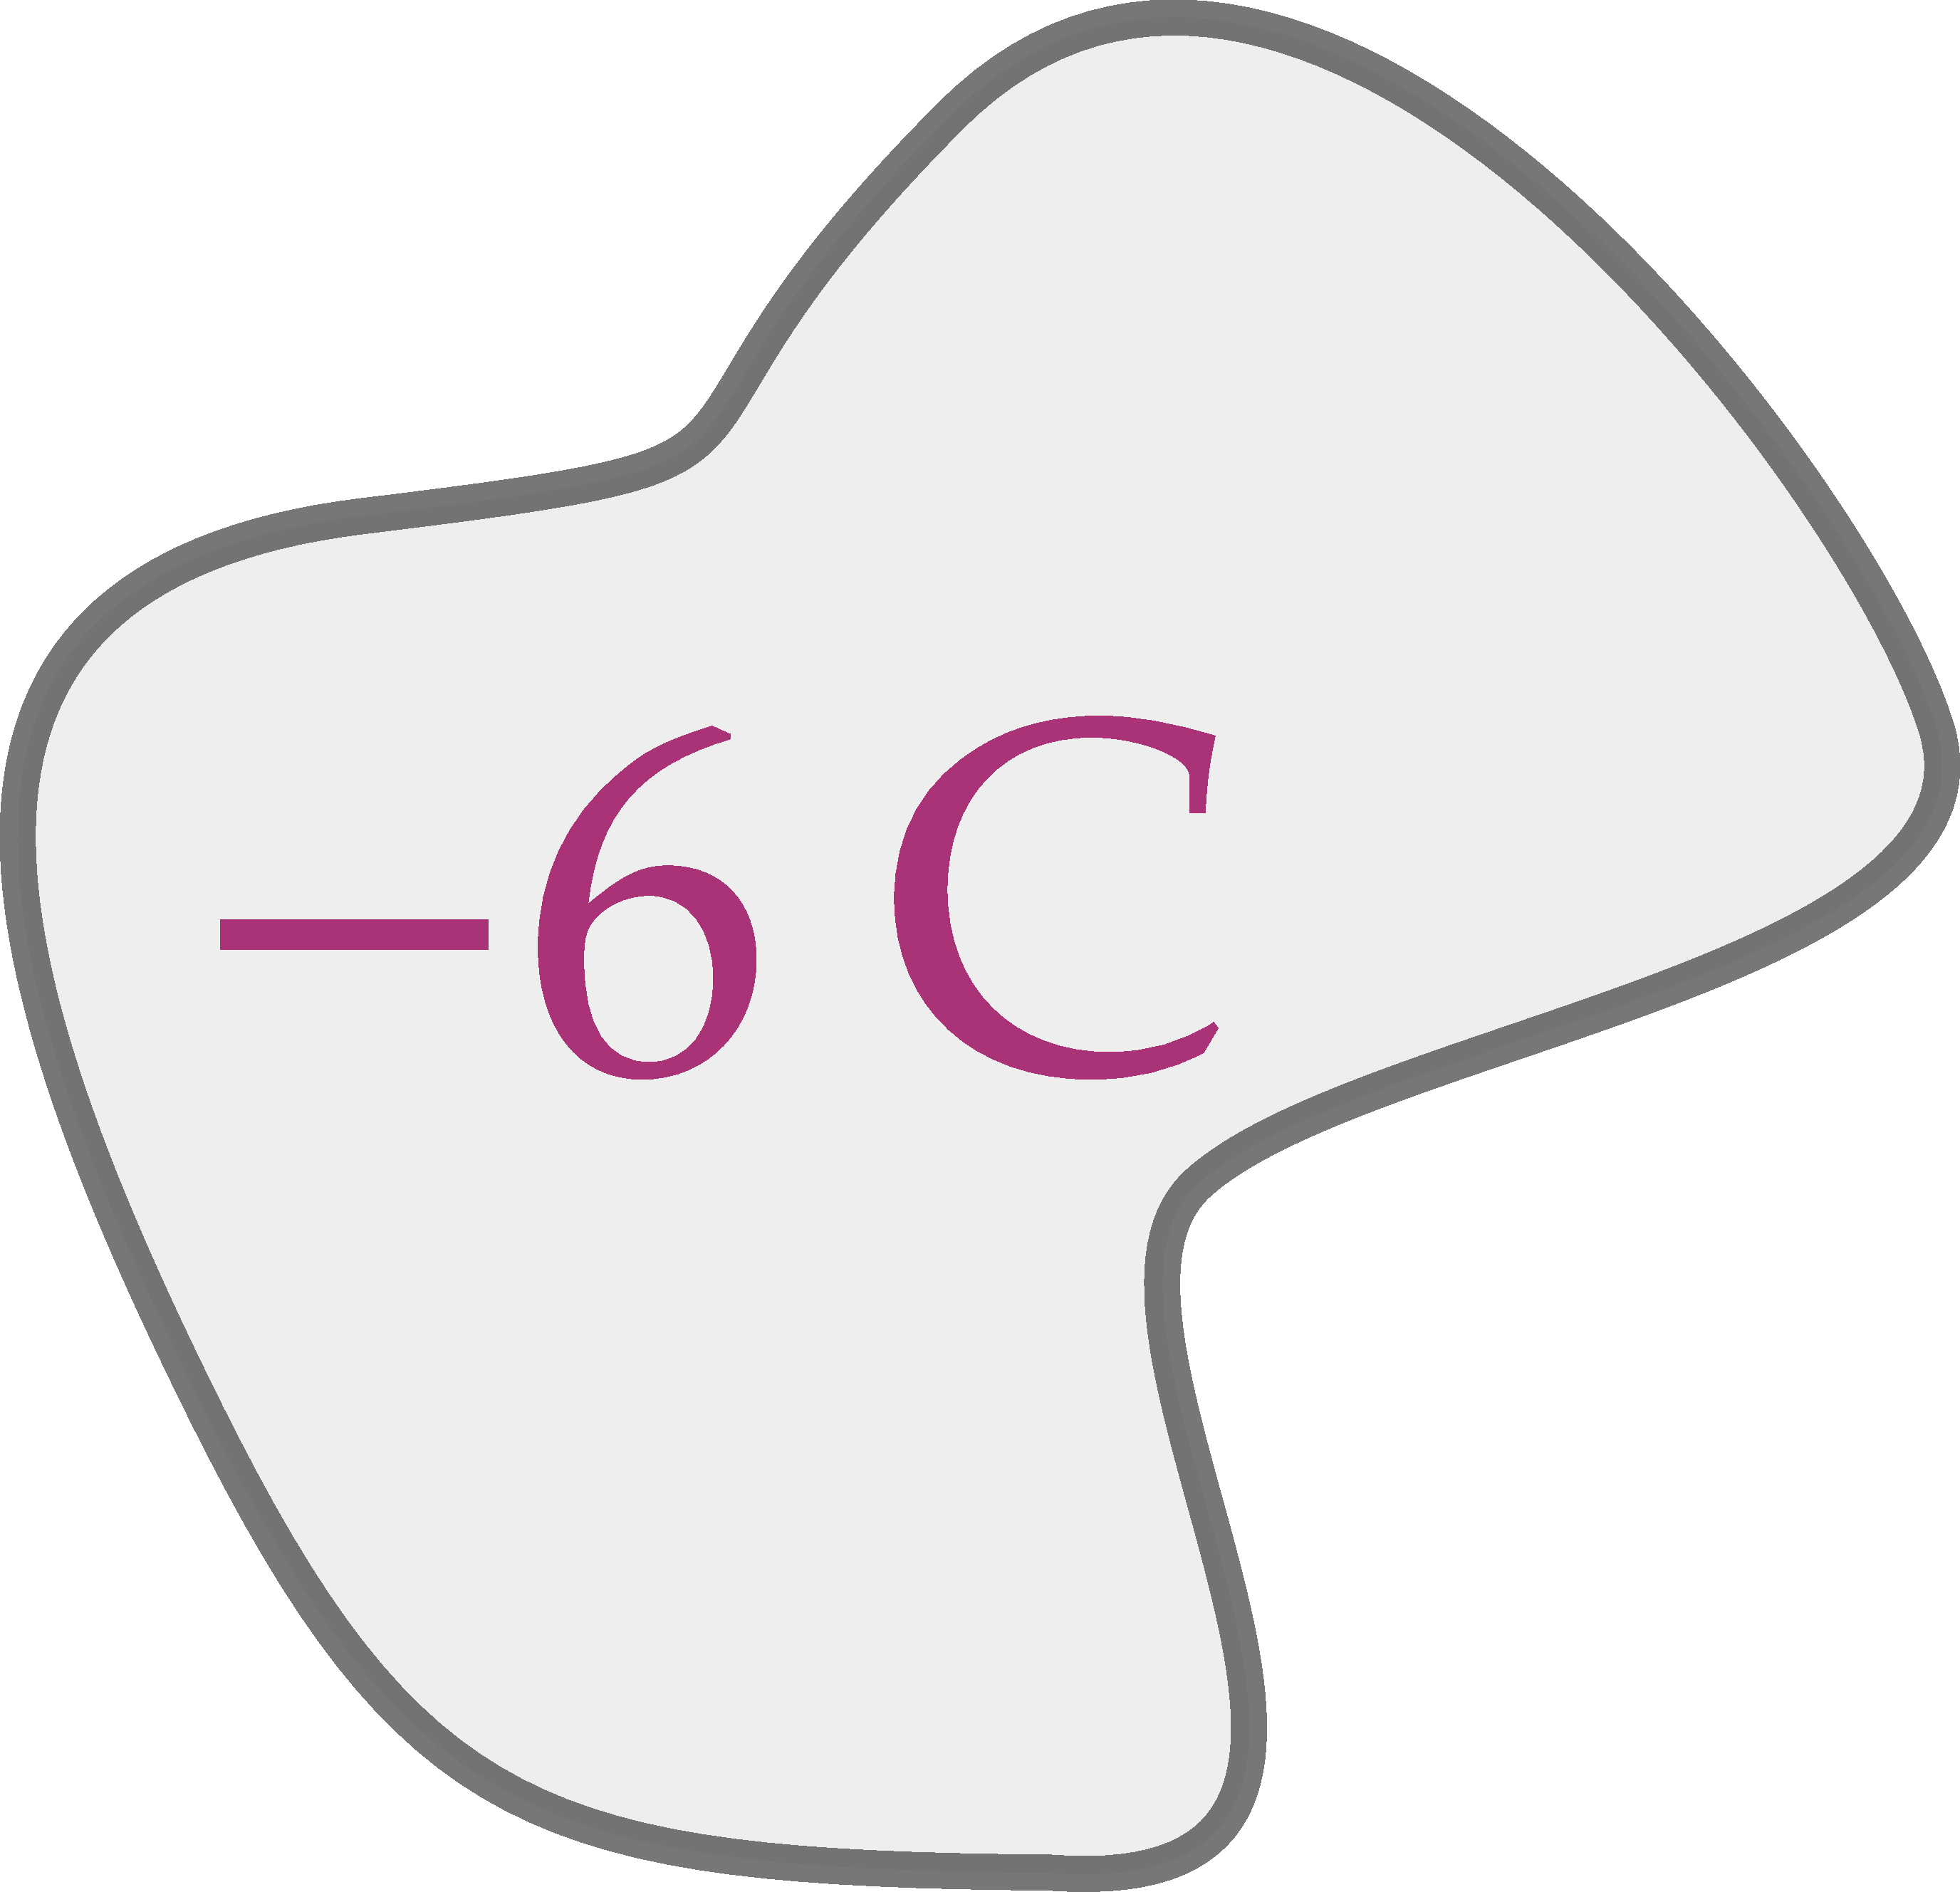
\includegraphics[align=c,width=0.5\linewidth]{images/volumeintegral_6C.pdf}
\\[\jot]\flushleftright\footnotesize\color{mpcolor}A region with a negative amount of charge%
}

\item We must not surmise that the amount of quantity is uniformly distributed within the volume. In fact there could be negative amounts of it in some subvolumes and positive in others. In particular,  even if there is a zero amount of quantity in a volume, some subvolumes could have non-zero amounts: some positive and some negative, so that the total is zero.
  % \begin{warning}
  %  Even if there is a zero amount of quantity in a volume, some subvolumes could have non-zero amounts: some positive and some negative, so that the total is zero.
  % \end{warning}
\end{itemize}

\bigskip

\begin{exercise}
  The volume content of matter in a particular volume is equal to \qty{36}{mol}. Can we conclude that the volume doesn't contain antimatter?
\end{exercise}


\subsection{Vector quantities}\label{sec:volintegral_vector}

A volume content for a vector quantity, for example momentum, can be represented as follows (we still simplify our visualization to two dimensions):
\begin{center}
  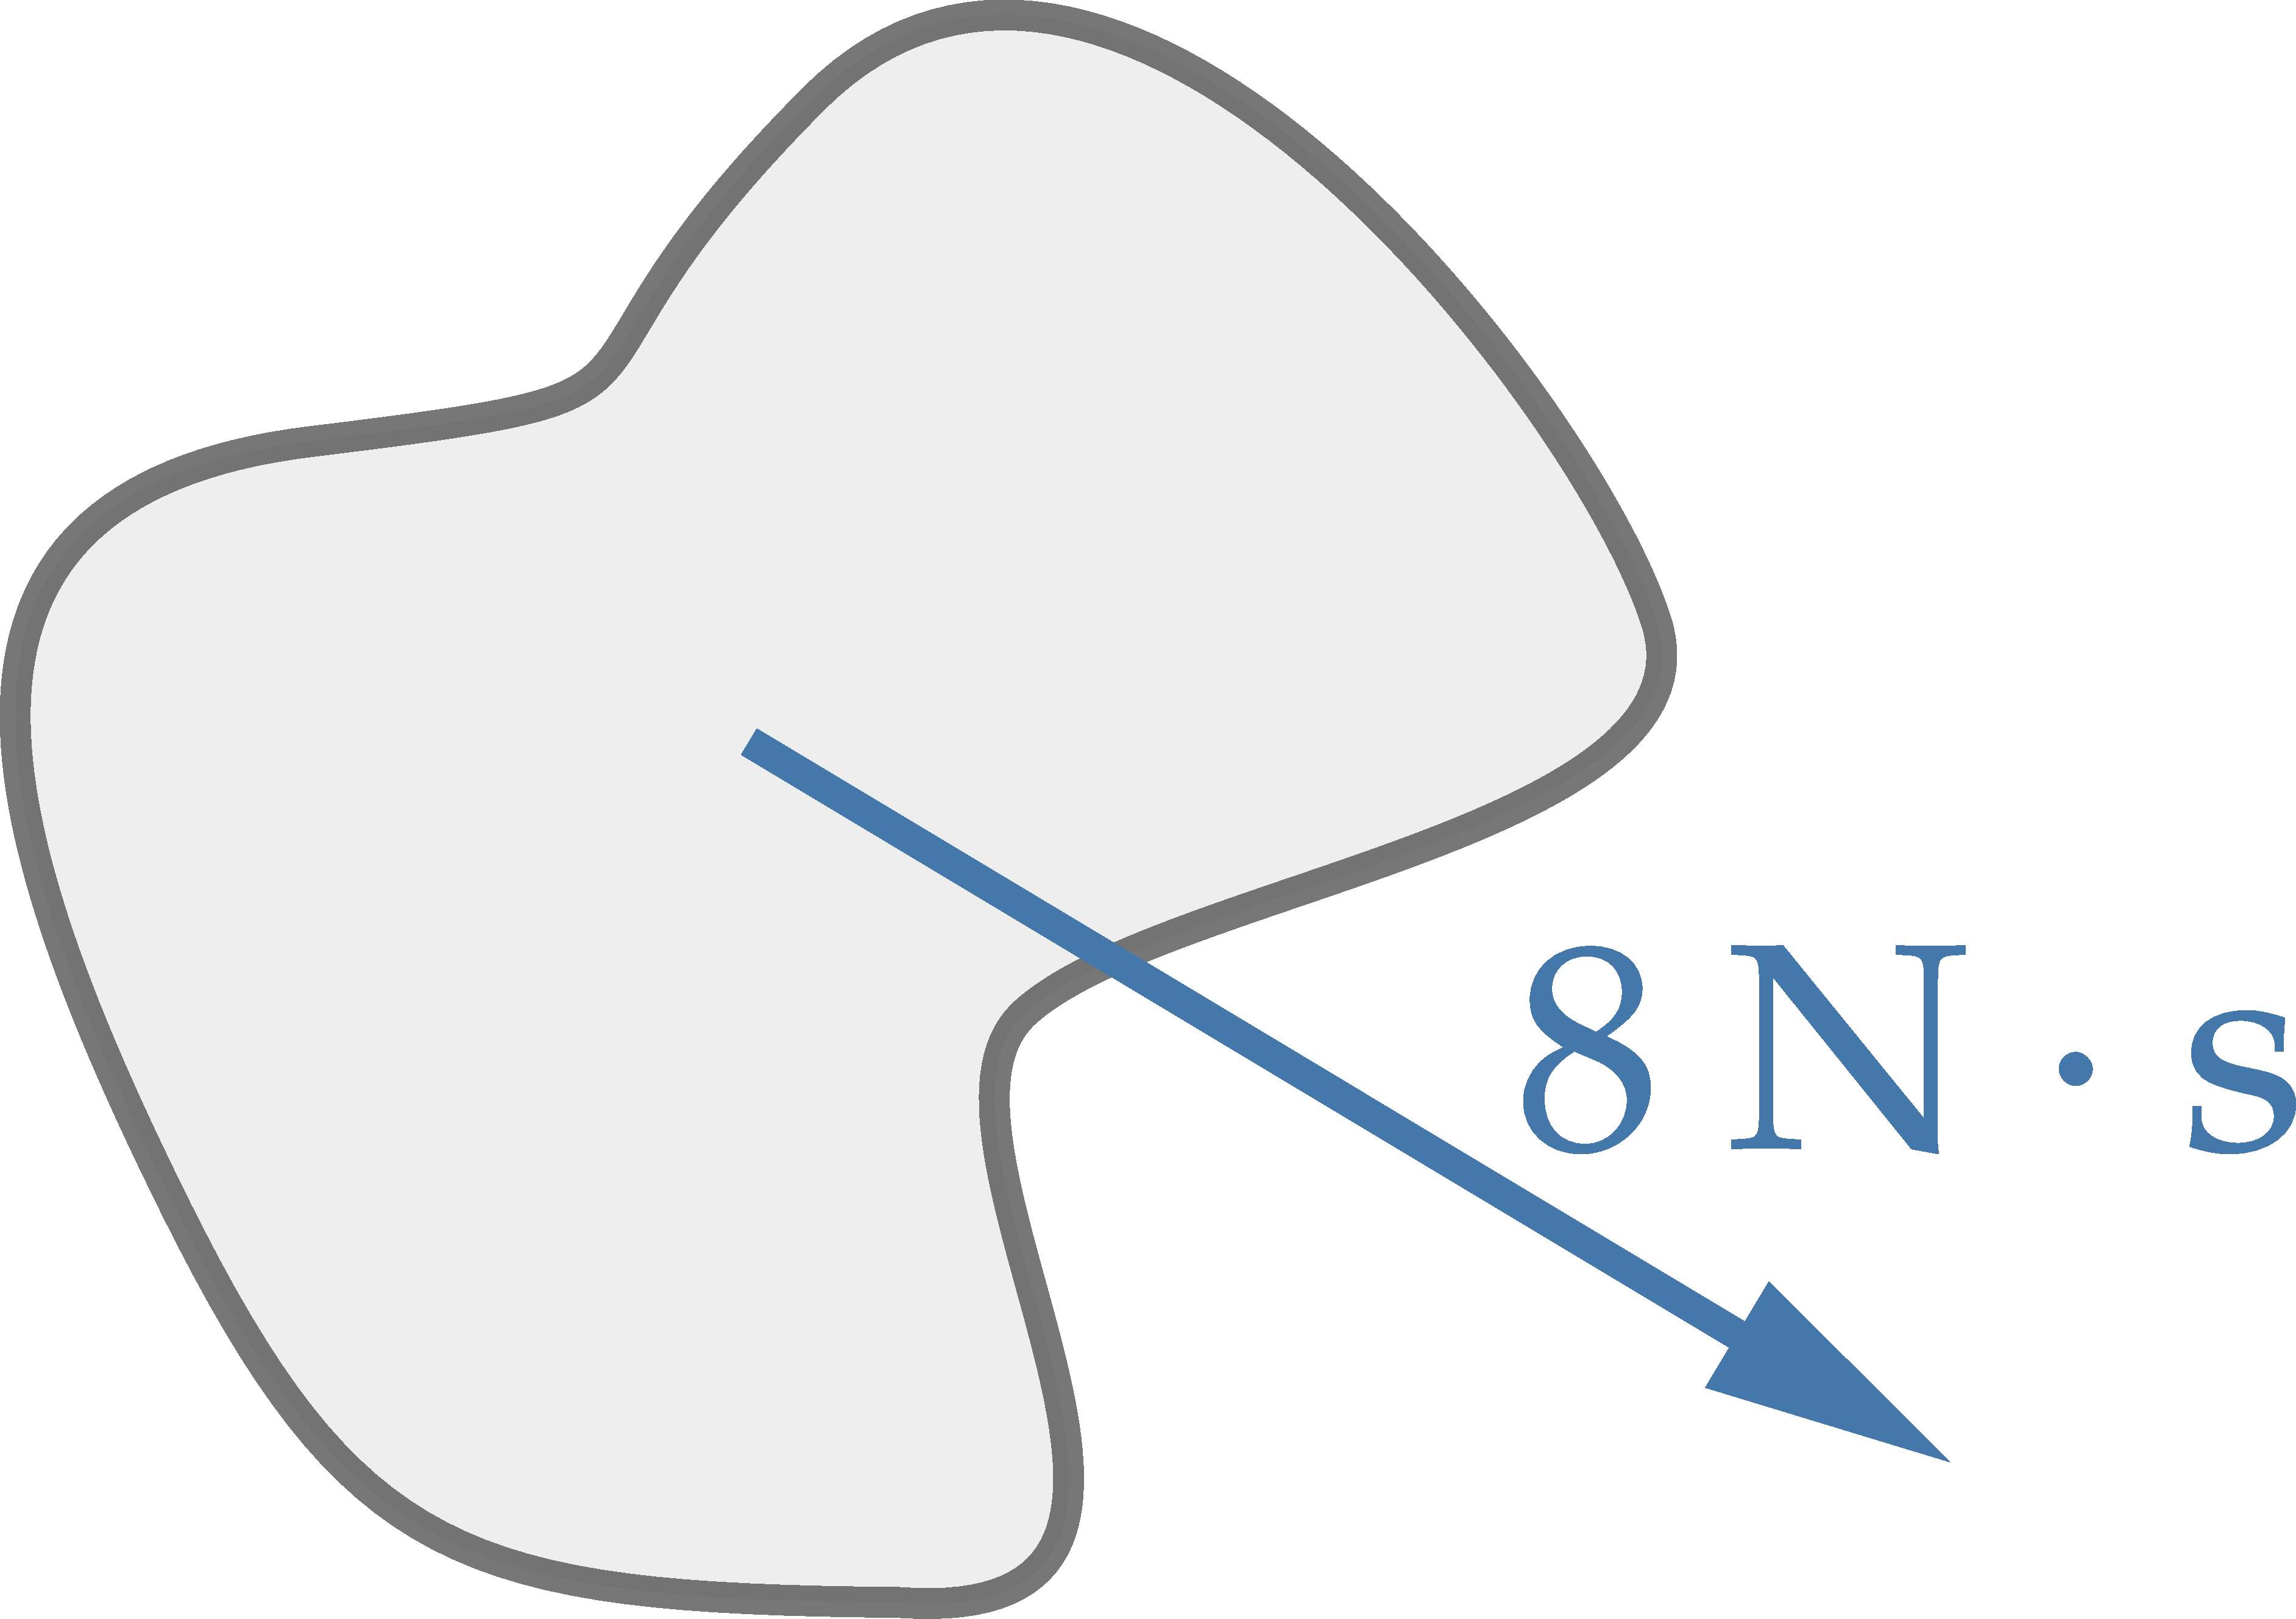
\includegraphics[height=7em]{images/volumeintegral_8Ns.pdf}
\end{center}
% \marginpar{\footnotesize
%   \begin{warning}%[Vector magnitudes are positive]
%     Remember that the \emph{magnitude} of a vector is always positive, and that\quad $\mathord{\mathcolor{purple}{\nwarrow}} = -1\cdot\mathord{\mathcolor{blue}{\searrow}}$
%   \end{warning}
% }
Momentum is a vector quantity, so the total amount in the volume above is a vector. The picture shows the direction and orientation of this vector, and the magnitude of \textcolor{blue}{\qty{8}{N\cdot s}}
is explicitly reported.
\begin{warning}[Vector magnitudes and opposite vectors]
  Remember that the \emph{magnitude} of a vector is always positive, and that\quad $\mathord{\mathcolor{purple}{\nwarrow}} = -1\cdot\mathord{\mathcolor{blue}{\searrow}}$
\end{warning}

The visual representation above is useful, if we keep in mind remarks analogous to the scalar case:
\begin{itemize}
\item This is a time snapshot.
\item\label{item:applicationpoint}The application point of the vector representing the volume content is unimportant: for instance, it doesn't need to be placed at the centre of the volume. The vector refers to the volume as a whole, not to some specific point within.
\item Different subvolumes could have amounts represented by different vectors; only the total vector is represented above.
\end{itemize}
This last remark is especially important when we discuss momentum and angular momentum. As an example, look at the side picture:%\fig~\ref{fig:nonzero_vector_subregions}:
\marginpar{\vspace{-3\baselineskip}\centering%
\includegraphics[width=0.5\linewidth]{images/volumeintegral_N_divided.pdf}
\\[\jot]\flushleftright\footnotesize\color{mpcolor}The whole region has zero volume content. The left and right subregions have non-zero and opposite volume contents.%
}
the volume content for the whole region is \emph{zero}, but its left and right subregions have \emph{non-zero and opposite} volume contents.
% \begin{figure}[h]\centering
%   \includegraphics[height=7em]{images/volumeintegral_N_divided.pdf}
%   \caption{The whole region has zero volume content. The left and right subregions have non-zero and opposite volume contents.}\label{fig:nonzero_vector_subregions}
% \end{figure}

\bigskip


\begin{exercise}
  Recall \emph{extensivity}, the third property of our seven main quantities: the amount in a volume consisting of separate volumes is equal to the total of the separate amounts.

We have a region consisting of two subregions; the amounts of momentum in each subregion are shown below.
  \begin{center}
    \includegraphics[width=0.5\linewidth]{images/exercise_momentumsum.pdf}
  \end{center}
  \begin{enumerate}[exerc]
  \item Write the total momentum in each subregion in component form, $(P_{x}, P_{y})$, according to the coordinate system shown.
  \item Calculate the momentum in the whole region; represent it graphically as vector and write it in component form.
  \end{enumerate}
\end{exercise}

\begin{extra}{Adding vectors in General Relativity}
  We are used to the idea of adding vectors placed at different points in space: we only have to move each vector, keeping it parallel to itself, to a common point; and then add them all at that point with the usual rule.

  This operation \emph{cannot} be done so simply in General Relativity: the notion of parallelism doesn't apply anymore in a simple way, owing to the curvature of spacetime. The addition would lead to different results depending on how we transported the vectors.

  But it is still possible to add the momentum of two different spatial regions, simply because \emph{momentum is defined with respect to a coordinate system}. This coordinate system selects, so to speak, a unique way to transport the momentum vectors to a common point. We are again reminded of the fact that \autoref{sec:energy_momentum_angmomentum_coords}{momentum is a coordinate-dependent quantity}.

  In General Relativity momentum is not really a vector, but just a special triplet of quantities.

  % How can this operation be possible in Newtonian mechanics and in practical applications, then? After all, General Relativity surely applies here! The answer is that the discrepancies of vector transportation are small enough in the neighbourhood of the Earth, as the curvature of spacetime is very small here.
\end{extra}


\section{Flux: scalar quantities}
\label{sec:intuition_fluxes_scalar}

\subsection{Crossing direction and reckoning of scalar fluxes}
\label{sec:flux_scalar_direction}

Earlier we considered the intuitive example of a \autoref{sec:choice_surfaces}{flow of people through an open door}. We may ask how many people crossed the door in a minute, but one more detail about this flow is important: \emph{in which direction did the people cross the door?} This detail is important because, for example, the door leads to a classroom and we need to keep track of how many seats are free. Then we need to know whether each person who crossed the door was \emph{entering} or \emph{leaving} the classroom, keeping track of how many additional people are in the classroom.

\marginpar{\vspace{-4\baselineskip}\centering%
\includegraphics[width=0.5\linewidth]{images/person_enter.pdf}
\\\flushleftright\footnotesize\color{mpcolor}According to the crossing direction indicated by the \textcolor{cyan}{blue wiggly arrow}, the person crossing the door counts as\enspace\enquote*{$+1$}.%

\bigskip

\centering%
\includegraphics[width=0.5\linewidth]{images/person_leave.pdf}
\\\flushleftright\footnotesize\color{mpcolor}According to the crossing direction indicated by the \textcolor{cyan}{blue wiggly arrow}, the person crossing the door counts as\enspace\enquote*{$-1$}.%
}%
In order to do this we can:
\begin{enumerate}[label=\arabic*.]
\item Assign a crossing direction to the door, for instance the direction from outside to inside the classroom.
\item Count as \enquote*{positive} each person who crosses the door in the chosen crossing direction, and as \enquote*{negative} each person who crosses the door in the opposite direction.
\end{enumerate}
The total of this counting tells us the \emph{net} number of people who crossed the door in the chosen direction. If we chose a crossing direction \emph{from outside to inside} the classroom, then this total is the net number of people who
\emph{entered} the classroom. If we chose a crossing direction \emph{from inside to outside} the classroom, then this total is the net number of people who
\emph{left} the classroom.

A flux therefore represents only a \emph{net} amount. Note also that this net amount can be \emph{negative}. For instance if we chose a crossing direction from outside to inside the classroom, and the net amount is $\num{-3}$, then it means that \emph{more people got out than in}. For instance, 9~persons may have entered the room during that minute, and 8~persons left. Or no person may have entered the room, and 3~persons left. In either case, the final situation is that those who got out in that minute were three more than those who got in.

One important aspect of this example and terminology is the following \emph{symmetry}:
\begin{itemize}
\item It is completely arbitrary which crossing direction we choose.
\item If we choose the other crossing direction, then the net amount will switch sign.
\end{itemize}
But the physical situation is still the same of course. Therefore the sentences
\begin{center}
  \enquote{\qty{+5}{persons} \emph{entered} the room}
\end{center}
and
\begin{center}
  \enquote{\qty{-5}{persons} \emph{left} the room}
\end{center}
% \begin{itemize}[nosep]
% \item \qty{+5}{persons} entered the room
% \item \qty{-5}{persons} entered the room
% \item \qty{-5}{persons} exited the room
% \item \qty{+5}{persons} exited the room
% \end{itemize}
are saying exactly the same thing.
% \marginpar{\vspace{-7em}\label{fig:newtonIII}%
% \footnotesize\raggedright\color{mpcolor}\enquote{\emph{\langnohyph{LEX~III. Actioni contrariam semper \amp\ {\ae}qualem esse reactionem\,: sive corporum duorum actiones in se mutuo semper esse {\ae}quales \amp\ in partes contrarias dirigi.}}}
%     \\\sourceatright{\cites{newton1687}}%\cites{newton1687_t1974}
% }%

\medskip

Consider a similar example, but instead of people, think of a quantity that can ordinarily also be \emph{negative}, such as electric charge. Let's choose the door-crossing direction from outside to inside the room. If we're told that a net amount \qty{-5}{C} of charge crossed the door in the chosen direction in one minute, then this could have happened in several ways:\noprelistbreak
\begin{itemize}[nosep]
\item a charge of \qty{-5}{C} was brought into the room
\item a charge of \qty{+5}{C} was brought out of the room
\item a charge of \qty{-2}{C} was brought into the room during the first \qty{30}{s}, and a charge of \qty{+3}{C} was brought out in the remaining \qty{30}{s}
\item a charge of \qty{-2}{C} was brought into the room during the whole minute, and a charge of \qty{+3}{C} was brought out at the same time
\item \textellipsis and many other possible combinations.
\end{itemize}
So the statement that \enquote{the flux of electric charge into the room was \qty{-5}{C} in one minute} does not tell us which of the situations above occurred.

\marginpar{\vspace{\baselineskip}\footnotesize\color{mpcolor}\enquote{\emph{%
      Fechner [in 1845] supposed every current to consist in a streaming of electric charges, the vitreous charges travelling in one direction, and the resinous charges, equal to them in magnitude and number, travelling in the opposite direction with equal velocity.}}\sourceatright{\cites{whittaker1910_r1951}}%
}%
In fact, ordinary electricity in wires was thought for some time to be associated with movements of negative \emph{and} positive charges in opposite directions. Today we know that it consists in the movement of negative charges only.

\medskip

The purpose of the previous examples is to make you aware of some fundamental aspects of what we call \enquote{flux}. These aspects are trivial but important when considering fluxes of physical quantities:
%
\begin{definition}{Fundamental aspects of flux}\label{def:symmetryflux}
  \begin{itemize}[nosep,shift]
  \item A flux in a particular surface-crossing direction only tells us the \emph{net} amount of substance that crosses the surface in that direction in a unit of time.

  \item A flux can be \emph{negative}.

  \item A flux in a particular surface-crossing direction is equivalent to a flux of \emph{opposite} sign in the \emph{opposite} crossing direction.
  \end{itemize}
\end{definition}

\begin{warning}[What a flux value does not tell]
  \begin{itemize}[nosep,shift]
  \item A flux value does not tell us the amount that crossed during shorter times or through different parts of the surface.

\item A flux value does not tell us whether the transfer of the quantity through the surface occurs because the quantity is flowing, or because the surface is moving, or both.
  \end{itemize}
\end{warning}




\subsection{Representation of scalar fluxes}
\label{sec:flux_scalar_representation}

% %
% \marginpar{\vspace{\baselineskip}\centering%
% \includegraphics[width=0.5\linewidth]{images/wiggly_arrow.pdf}
% \\[\jot]\flushleftright\footnotesize\color{mpcolor}We'll use wiggly arrows like this one  to indicate a \emph{crossing direction} through a surface. Keep in mind that these arrows \emph{are not vectors}! They don't have a \enquote*{magnitude} or \enquote*{components}.%
% }
% %

How can we graphically represent the flux of a quantity, in a way that takes care of all its fundamental aspects?

First let's consider a surface through which we're measuring a flux, at a particular instant of time. Here it is represented as line, removing one spatial dimension to simplify the drawing:\noprelistbreak
\begin{center}
  \medskip
  \includegraphics[height=5em]{images/surface_tilted_nocross.pdf}
\end{center}
Keep in mind that the surface could have any other shape, and could also be in motion.

Let's indicate a crossing direction through the surface by one or more wiggly arrows:\noprelistbreak
\begin{center}
  \medskip
  \includegraphics[height=5em]{images/surface_tilted_crossright.pdf}
\end{center}
Keep in mind that these arrows \emph{are not vectors}! They don't have a \enquote*{magnitude} or \enquote*{components}. They simply indicate a sense in which we imagine the surface to be crossed. We could also have used only one wiggly arrow or three instead of two.

A flux of \num{+5} of some scalar quantity through the surface, in the first crossing direction, can then be depicted as follows:\noprelistbreak
\begin{center}
  \medskip
  \includegraphics[height=5em]{images/flux_plus5c.pdf}
\end{center}
This picture says that a net amount of \num{5} has crossed the surface from the left to the right side, in a unit of time. This also means that in a unit of time a net amount of \num{5} has \enquote{disappeared} from the left side of the surface and \enquote{appeared} on the right side.

\medskip

Now consider the opposite crossing direction, depicted like this:\noprelistbreak
\begin{center}
  \medskip
  \includegraphics[height=5em]{images/surface_tilted_crossleft.pdf}
\end{center}
Because of the symmetry of fluxes, we can say that the flux equals \num{-5} in this opposite direction. We depict this as follows:\noprelistbreak
\begin{center}
  \medskip
  \includegraphics[height=5em]{images/flux_minus5c.pdf}
\end{center}
This picture says that a net amount of \num{-5} has crossed the surface from the right to the left side, in a unit of time. This also means that a net amount of \num{-5} has \enquote{disappeared} from the left side of the surface and \enquote{appeared} on the right side, in a unit of time.

But this is indeed exactly the same situation as before. \emph{Both pictures therefore represent the same flux}:\noprelistbreak
\begin{center}\label{fig:scalar_fluxes}
  \bigskip
  \hspace*{\fill}
  \includegraphics[align=c,height=6em]{images/flux_plus5c.pdf}
\qquad{\small is exactly the same as}\qquad
\includegraphics[align=c,height=6em]{images/flux_minus5c.pdf}
%\hfill\includegraphics[height=6em]{images/flux_minusplus5.pdf}
\hspace*{\fill}
\end{center}

\textbf{It is extremely important that you remember that the two kinds of picture above are completely equivalent}. You can always mentally switch from one to the other. A flux in one crossing direction is exactly the same as a flux with opposite sign in the opposite direction.

The two equivalent pictures do \emph{not} say that a given amount is \emph{only} moving from left to right, or vice versa; we have seen that in general we don't know this. Both pictures say that on the left side the amount of quantity has changed by \num{-5}, and on the right side by \num{+5}. In these notes we shall usually display only one of these two equivalent representations.

% The third picture tries to avoid this misleading interpretation by not showing any arrows; it is meant to represent that on the left side the amount of quantity has changed by \textcolor{purple}{\num{-5}}, and on the right side by \textcolor{blue}{\num{+5}}. But also this picture may be misleading in suggesting that \num{+5} crossed left-to-right \emph{and} \num{-5} crossed right-to-left, for a total of \num{+10} left-to-right. Or vice versa it may lead you to sum up the two numbers, in which case you'll always obtain zero! % *****

% The third representation above has one more advantage. Remember that \autoref{sec:choice_surfaces}{a flux through a surface may occur because the surface itself is moving}. The wiggly arrows in the first two representations above may misleadingly suggest that some amount of quantity is \enquote{moving} in their direction, or that the surface itself is moving in that direction. The third, arrow-less representation is less misleading.


\subsection{Scalar fluxes through different surfaces}
\label{sec:surface_change_scalar}

What happens to the value of a flux through a surface, if we consider a \emph{different} surface, maybe intersecting the original one? It's important to keep in mind that
\begin{itemize}[nosep]
\item A flux refers only to a specific surface.
\item The fluxes through two distinct surfaces can be very different, even if the two surfaces are quite close.
\item The flux depends on the motion of the surface. So if we consider the same surface but with a different instantaneous motion, then the flux may be very different.
\end{itemize}


Consider for instance the picture on the side.
%
\marginpar{\vspace{-5\baselineskip}\centering\includegraphics[width=\linewidth]{images/two_surfaces_flux.pdf}%
}%
It depicts two intersecting surfaces (as usual simplified by removing one dimension) and two chosen crossing directions on them. The crossing directions are both roughly rightward. Yet the energy flux through the \textcolor{blue}{solid blue surface} is \textcolor{blue}{\qty{+5}{J/s}}, whereas the energy flux through the \textcolor{purple}{dashed red surface} is \textcolor{purple}{\qty{-1}{J/s}}.

% As another example,
% % %
% % \marginpar{\vspace{-2\baselineskip}\centering\includegraphics[width=0.67\linewidth]{images/two_surfaces_flux_eq.pdf}%
% % }%
% the second side picture shows two similar intersecting surfaces, one fully vertical in \textcolor{blue}{solid blue}, and one fully horizontal in \textcolor{purple}{dashed red}. The energy flux through the first in a rightward direction is \textcolor{blue}{\qty{+3}{J/s}}, and so is the energy flux in an upward direction through the second surface.

\smallskip

There is, however, a relation between the fluxes through surfaces that share a common point. If we know the flux through \emph{three different, small, static} surfaces having a common point, then we can find the flux through any other \emph{small, static} surface passing through that same point. This possibility leads to the representation of flux through a small surface as a \emph{vector}, called \enquote*{flux-density vector}. In these notes we shall not consider flux densities and their vector representation.
% ***** change this if they are added in an "advanced" part.


\subsection{Flux units: scalar quantities}

Remember that the flux of a quantity is defined as an amount of that quantity \emph{per time lapse}. Therefore the physical dimension of the flux is
\begin{equation*}
  \frac{\textsf{quantity}}{\textsf{time}}
\end{equation*}
and its units will be the units of the quantity divided by seconds:
\begin{definition}{units of fluxes of the four scalar quantities}
  \centering
  \begin{tabular*}{\linewidth}{@{\extracolsep{\fill}}lccccc}
    \textbf{quantity}& matter & energy &
    \begin{minipage}{3em}
      \centering electric\\charge
    \end{minipage}
    &
        \begin{minipage}{4em}
      \centering magnetic\\field
    \end{minipage}
 & entropy
    \\[3\jot]
    \textbf{flux units}& \unit{mol/s} & \unit{J/s} & \unit{C/s} & \unit{Wb/s} & \unit{J/(K\cdot s)}
    \\[2\jot]
    \textbf{equivalent units}& \emph{watt} & \emph{ampere} \unit{A} & \unit{W} & \emph{volt} \unit{V} &
  \end{tabular*}
%  \caption{Units of scalar fluxes}
  \label{tab:fluxes_scalar_units}
\end{definition}

\bigskip

After our discussion about the peculiarity of fluxes it's quite easy to work with the fluxes of the four main scalar quantities: matter, electric charge, energy, entropy. Let us add some reminders and remarks about the fluxes of matter and energy.


\subsubsection{Matter flux}
\label{sec:matter_flux}

Remember that \emph{anti}matter \enquote{counts as \num{-1}} for calculating amounts of matter. If \qty{1}{mol} of positrons (anti-electrons) crosses a surface from left to right in \qty{1}{s}, the left-to-right flux of electrons equals \qty{-1}{mol/s} -- note the minus sign. The fact that antimatter is given special names can lead to ambiguities. For instance, if someone asks \enquote{what's the left-to-right flux of \emph{positrons}?}, maybe we should answer \enquote{\qty{1}{mol/s}}, since the question concerned specifically positrons. It's somewhat like asking \enquote{what's the flux of \emph{negative} electric charge?}. In these ambiguous situations it's best to add some explanatory words.

\subsubsection{Energy flux}
\label{sec:energy_flux}
We already mentioned that \autoref{sec:forms_energy}{energy flux can be categorized into different kinds}, depending on whether there are fluxes of other quantities through the same surface. We study the exact definitions and formulae later on. The total flux is given by the sum of all these kinds. For instance, through a horizontal surface we can have a downward energy flux of \qty{3}{J/s} as \emph{heat}, and a downward flux of \qty{-1}{J/s} as \emph{work}. The total downward flux is then \qty{2}{J/s}. The energy flux that you will calculate in the fourth exercise below is called \emph{energy convection}.


\begin{exercise}
    For each question, answer in an \emph{unambiguous} way and sketch a picture representing the flux.
  \begin{enumerate}[exerc]
  \item The two sides of a particular surface are called \enquote*{up} and \enquote*{down}. During \qty{0.2}{s}, an energy of \qty{+3}{J} flows from the up-side to the down-side, and an energy of \qty{-4}{J} flows from the down-side to the up-side. How much is the flux of energy through the surface?
  \item Through the same surface, at a later time, \qty{2}{mol} of neutrons flow from the up- to the down- side in \qty{0.01}{s}, and \qty{2}{mol} of neutrons flow from the down- to the up-side during the same time. How much is the flux of matter through the surface?
  \item The two sides of a surface are called \enquote*{in} and \enquote*{out}. During \qty{0.01}{s} there is a flow of \num{1000} electrons from the in-side to the out-side, and also a flow of \num{1000} \emph{positrons} (anti-electrons) in the same direction. How much is the flux of matter through the surface?
  \item The side picture shows a \textcolor{green}{surface} moving from left to right at a (constant) velocity of \qty{1}{m/s}. The space to its right has two static regions with some amount of \textcolor{blue}{energy} as shown (there's no energy behind to the left of the surface). How much is the flux of energy through the surface in \qty{1}{s}?
  \end{enumerate}
\end{exercise}
%
\marginpar{\vspace{-6\baselineskip}\centering\includegraphics[width=\linewidth]{images/surfacemoving_J.pdf}
}%



\section{Flux: vector quantities}
\label{sec:intuition_fluxes_vector}

\subsection{Crossing direction and reckoning of vector fluxes}
\label{sec:flux_vector_direction}

The flux of a vector quantity is also a vector, because it is given by an amount of that quantity, which is a vector, divided by time, which is a scalar. We can see it as three fluxes of three scalar quantities.

The discussion about the \autoref{sec:flux_scalar_direction}{choice of crossing direction and the symmetry of fluxes} that we made in the case of the flux of a scalar quantity, also applies in an analogous way to the flux of a vector quantity. For instance, if the flux of momentum through a surface in a particular crossing direction is
\begin{equation*}
  (-21, 25, 0)\:\unit{N} \ ,
\end{equation*}
then if we choose the opposite crossing direction the flux is
\begin{equation*}
  -(-21, 25, 0)\:\unit{N} = (+21, -25, 0)\:\unit{N}\ .
\end{equation*}

If we think of vectors as arrows, we must only remember that a minus sign changes their orientation:\noprelistbreak
\begin{equation*}
  \mathord{\nwarrow} \mathrel{\enspace=\enspace} -1\cdot\mathord{\searrow}
\end{equation*}


\subsection{Representation of vector fluxes}
\label{sec:flux_vector_representation}

The graphical representation of the flux of a vector quantity is also analogous to \autoref{sec:flux_scalar_representation}{that for the flux of a scalar quantity}.


Take for instance the following surface with a specified crossing direction:\noprelistbreak
\begin{center}
  \medskip
  \includegraphics[height=5em]{images/surface_tilted_crossright.pdf}
\end{center}
Suppose that with respect to this crossing direction the flux the vector of components\enspace$\mathcolor{blue}{(21, -25, 0)}$:\noprelistbreak
\begin{center}
  \medskip
  \includegraphics[height=4em]{images/vec_NW.pdf}
\end{center}
Then we can depict this flux as follows:\noprelistbreak
\begin{center}
  \medskip
\includegraphics[height=6em]{images/flux_vec_right.pdf}%
\end{center}
This picture says that a net vector amount\enspace\includegraphics[align=c,height=1.5em]{images/vec_NW.pdf}\enspace
has crossed the surface from the left to the right side, in a unit of time. This also means that in a unit of time a net vector amount\enspace\includegraphics[align=c,height=1.5em]{images/vec_NW.pdf}\enspace has \enquote{disappeared} from the left side of the surface and \enquote{appeared} on the right side. (Remember that the \textcolor{cyan}{wavy arrows} are \emph{not} vectors: they only represent a crossing direction.)

If we instead choose the opposite crossing direction:\noprelistbreak
\begin{center}
  \medskip
  \includegraphics[height=5em]{images/surface_tilted_crossleft.pdf}
\end{center}
then the same flux is represented by the opposite vector:\noprelistbreak
\begin{center}
  \medskip
  \includegraphics[height=4em]{images/flux_vec_left.pdf}
\end{center}
This picture says that a net vector amount\enspace\includegraphics[align=c,height=1.5em]{images/vec_SE.pdf}\enspace
has crossed the surface from the right to the left side, in a unit of time. This also means that in a unit of time a net vector amount\enspace\includegraphics[align=c,height=1.5em]{images/vec_SE.pdf}\enspace has \enquote{disappeared} from the right side of the surface and \enquote{appeared} on the left side. But this is the same flux as before, because\enspace\includegraphics[align=c,height=1.5em]{images/vec_SE.pdf}${}= -{}$\includegraphics[align=c,height=1.5em]{images/vec_NW.pdf}.

\emph{Both pictures therefore represent the same flux}:\noprelistbreak
\begin{center}\label{fig:scalar_fluxes}
  \bigskip
\hspace*{\fill}\includegraphics[align=c,height=6em]{images/flux_vec_right.pdf}
\qquad{\small is exactly the same as}\qquad
\includegraphics[align=c,height=6em]{images/flux_vec_left.pdf}
%\hfill\includegraphics[height=6em]{images/flux_minusplus5.pdf}
\hspace*{\fill}
\end{center}

% %
% \marginpar{\vspace{-8\baselineskip}\centering\includegraphics[width=0.5\linewidth]{images/vectorfluxanim.png}%
% \\[\jot]\flushleftright\footnotesize\color{mpcolor}Imagine the \textcolor{blue}{blue upper arrows} moving from left to right, and the \textcolor{purple}{red lower arrows} moving from right to left. \furl{https://pglpm.github.io/7wonders/media/vectorfluxanimsin.webp}{Animated version here}.%
% }%
% As a mental image of a vector flux, you can imagine a moving collection of identical arrows crossing the surface in one direction, together with a moving collection of opposite arrows crossing the surface in the opposite direction.
% \furl{https://pglpm.github.io/7wonders/media/vectorfluxanimsin.webp}{See this link} as an example.

\smallskip

We can of course also explicitly write the numerical values of the vector components:\noprelistbreak
\begin{center}\label{fig:scalar_fluxes}
  \bigskip
  \hspace*{\fill}
  \includegraphics[align=c,height=6em]{images/flux_vec_right_num.pdf}
\qquad{\small is exactly the same as}\qquad
\includegraphics[align=c,height=6em]{images/flux_vec_left_num.pdf}
%\hfill\includegraphics[height=6em]{images/flux_minusplus5.pdf}
\hspace*{\fill}
\end{center}
Both pictures say that the $x$-component of the quantity has changed on the right side of the surface by \num{-21}, and on the left side by \num{+21}; the $y$-component  has changed on the right side by \num{+25}, and on the left side by \num{-25}; and the $z$-component has not changed on either side.

\medskip

An important aspect of vector fluxes that we must try not to get confused about is the application point of the vector (the base point of the arrow). Just as for \autoref{item:applicationpoint}{vector volume contents}, \textbf{the application point of the vector representing the flux is unimportant. The vector refers to one side of the surface as a whole.} So the following four pictures represent exactly the same flux:\noprelistbreak
\begin{center}\label{fig:scalar_fluxes}
  \bigskip
  \hspace*{\fill}
  \includegraphics[align=c,height=6em]{images/flux_vec_right.pdf}
\hfill
\includegraphics[align=c,height=6em]{images/flux_vec_right_alt.pdf}
\hfill
\includegraphics[align=c,height=6em]{images/flux_vec_left.pdf}
\hfill
\includegraphics[align=c,height=6em]{images/flux_vec_left_alt.pdf}
\hspace*{\fill}
\end{center}

\medskip

\begin{exercise}
  A horizontal surface is given, and there is a flux of a vector quantity through it (for the moment we neglect units):
  \begin{enumerate}[label=\arabic*.]
  \item If we take the \emph{downward} crossing direction as \enquote*{positive}, the flux $xyz$-components are $(5,5,0)$. Represent this flux graphically, in the way discussed in the present section. Use the coordinate system\enspace\includegraphics[align=c,height=2em]{images/coords_xy.pdf}\enspace were $y$ points upward.
  \item Taking the same crossing direction, represent graphically the flux $(0,-2,0)$ instead.
  \item Taking the same downward crossing direction, we are now told that there is a flux with components $(1,-2,3)$. What are the components of this flux if we take the \emph{upward} crossing direction as positive?
  \end{enumerate}
\end{exercise}


\medskip

\subsection{Vector fluxes through different surfaces}
\label{sec:surface_change_vector}

We saw that the flux of a scalar quantity can be very different if we take a slightly different surface, or the same surface with a different motion. The same is true of the flux of a vector quantity: in particular, \textbf{the vectors representing the fluxes through two slightly different surfaces can point in completely different directions}.

Here is an example. Take a fixed point $P$. Now take a small vertical surface passing through $P$, and choose a crossing direction from left to right. The flux of a vector quantity (momentum for example) through this quantity could be as in this picture:
\begin{center}
  \includegraphics[align=c,scale=0.08]{images/skewfluxPx.pdf}
% \makebox[0pt][c]{\hspace*{0.5\linewidth}\footnotesize(\furl{https://pglpm.github.io/7wonders/media/skewflux1.webp}{animated version})}
\end{center}
this flux has components $\mathcolor{blue}{(9,-6,0)}$, with magnitude around \num{10.8}.

Now forget about that surface, and take instead a small horizontal surface passing through the same point $P$, and upward crossing direction. The flux of the same quantity through this new surface could be as in this picture:
\begin{center}
  \includegraphics[align=c,scale=0.08]{images/skewfluxPy.pdf}
% \makebox[0pt][c]{\hspace*{0.5\linewidth}\footnotesize(\furl{https://pglpm.github.io/7wonders/media/skewflux2.webp}{animated version})}
\end{center}
it has components $\mathcolor{blue}{(-6,-3,0)}$, with magnitude around \num{6.7}.

Clearly the two vector fluxes through these two surfaces are completely different: they point in different directions and have different magnitudes.

% If we have a vector flux through a particular surface, and we're asked about the flux through a different surface, we might be tempted to \enquote{move} through the new surface the vectors representing the flux through the old one. \emph{We must fully resist this temptation}. It only leads to mistakes.
\begin{warning}[Each surface has a unique flux]
  A flux, scalar or vector, through a particular surface, in general doesn't tell us anything about the flux though another surface, nor about the flux through the same surface but with a different instantaneous motion.
\end{warning}

\subsection{Flux units: vector quantities}

Also for vector quantities the physical dimension of the flux is
\begin{equation*}
  \frac{\textsf{quantity}}{\textsf{time}}
\end{equation*}
and its units will be the units of the quantity divided by seconds:
\begin{definition}{units of fluxes of the three vector quantities}
  \centering
  \begin{tabular*}{\linewidth}{@{\extracolsep{\fill}}lccc}
    \textbf{quantity}& momentum & ang. momentum
    \\[2\jot]
    \textbf{flux units}& \unit{N} & \unit{N\,m}
    \\[2\jot]
    \textbf{equivalent units}& \unit{kg\,m/s}  & \unit{kg\,m^2/s}
  \end{tabular*}
%  \caption{Units of scalar fluxes}
  \label{tab:fluxes_vector_units}
\end{definition}


\section{Flux of momentum: force}
\label{sec:force_is_flux}

We already mentioned that \autoref{sec:intro_momentum}{\textbf{flux of momentum is what we call \enquote*{force}}}. Owing to the importance of the notion of \emph{force} in the many branches of physics which rely on Newtonian mechanics, we must discuss this connection in depth. This connection, as well as the connection to Newton's laws, will become even clearer when we discuss the balance of momentum in \chap\,\ref{cha:bal_momentum}.

\subsection{Units}
\label{sec:units_momflux}

Recall that \autoref{sec:intro_momentum}{momentum can be measured in newton-seconds, \enquote*{\unit{N\cdot s}}}. Its flux, being a momentum per unit time, is therefore measured in newtons, \enquote*{\unit{N}}.

\subsection{Visualizing force as flux of momentum}
\label{sec:visualize_force}

The notion of force is very intuitive. We associate it to the sensations that we feel in our skin, flesh, bones when, for instance, we push against a wall, twist a door knob, push backwards on the ground with our feet to run or jump, or other similar actions. Force is typically represented by a vector, having the direction and orientation of the \enquote{push} or \enquote{pull}, and a magnitude expressing its intensity. \emph{Such a force vector is exactly the vector expressing the flux of momentum}. The two are the same. A force can therefore be also visualized as a flow of momentum. This representation can be illuminating in some physical problems.

As a concrete example, imagine a person pushing against a wall, as in the side picture. In terms of force, we say that \emph{the person's head is exerting a force on the wall}; the vector that represents this pushing force, the \textcolor{purple}{purple arrow} in the picture, has a person$\to$wall orientation.
%
\marginpar{\vspace{-8\baselineskip}\centering\includegraphics[width=0.75\linewidth]{images/person_push_force.pdf}%
}%
% \begin{center}
%     \includegraphics[height=8em]{images/person_push_force.pdf}
% \end{center}

To understand force in terms of momentum flux, let's consider an imaginary surface separating the person and the wall; the \textcolor{yellow}{yellow line} in the pictures below. If we choose a person$\rightsquigarrow$wall crossing direction, indicated by the \textcolor{red}{wiggly red arrow} in the following picture, then the momentum flux has a person$\rightarrow$wall orientation:\noprelistbreak
\begin{center}
  \includegraphics[height=6em]{images/person_push_flux_right.pdf}
\end{center}
This picture says: on the side of the wall, an amount momentum is being added at a given rate; this momentum has a person$\rightarrow$wall orientation.

Because of the symmetry of flux, if we instead choose a wall$\rightsquigarrow$person crossing direction for the separating surface, then the momentum flux has opposite orientation:\noprelistbreak
\begin{center}
  \includegraphics[height=6em]{images/person_push_flux_left.pdf}
\end{center}
This picture says: on the side of the person's head, momentum is being added at a given rate; this momentum has a wall$\rightarrow$person orientation.

Since force and momentum flux are the same thing, the last picture tells us that \emph{the wall is exerting a force on the person's head}; the vector that represents this opposite pushing force has a wall$\to$person orientation. -- But this is \emph{Newton's Third Law}! This example therefore shows that Newton's third law is the expression of the symmetry of fluxes. We shall discuss this fact in the next section.

\medskip

Now let's consider an example involving pulling instead of pushing. Imagine a person pulling a rope fastened somewhere, as in the side picture. In terms of force we say that \emph{the person is exerting a force on the rope}; the vector that represents this force has a rope$\rightarrow$person orientation.
%
\marginpar{\vspace{-4\baselineskip}\centering\includegraphics[width=\linewidth]{images/person_pull_force.pdf}%
}%
% This can be depicted like this:\noprelistbreak
% \begin{center}
%     \includegraphics[height=6em]{images/person_pull_force.pdf}
% \end{center}

In terms of momentum flux, let's consider an imaginary vertical surface between the person's hand and the rope; the \textcolor{yellow}{yellow line} in the pictures below. If we choose an arm$\rightsquigarrow$rope crossing direction, indicated by the \textcolor{red}{wiggly red arrow}, then the momentum flux has a rope$\rightarrow$arm orientation; note the difference from the previous example:\noprelistbreak
\begin{center}
  \includegraphics[height=6em]{images/person_pull_flux_right.pdf}
\end{center}
This picture says: on the side of the rope, an amount momentum is being added at a given rate; this momentum has a rope$\rightarrow$arm orientation.

But again this momentum flux and the previous picture are \emph{completely equivalent} to the following ones, by the symmetry of fluxes:\noprelistbreak
\begin{center}
  \includegraphics[height=6em]{images/person_pull_flux_left.pdf}
\end{center}
This picture says: on the side of the arm, an amount momentum is being added at a given rate; this momentum has an arm$\rightarrow$rope orientation. Again we find Newton's third law: the rope is exerting a force on the person's arm; the vector that represents this opposite pushing force has a rope$\to$arm orientation.

\medskip

A final example illustrates a situation in between the previous two. Consider the foot of a running person, as it pushes on the ground. In terms of momentum flux, consider an imaginary horizontal surface between the runner's foot and the ground; the horizontal \textcolor{yellow}{yellow line} in the pictures below. If we choose a downward crossing direction, the momentum flux is oriented diagonally, downward and backwards, towards the rear of the foot. Because of the symmetry of fluxes, if we choose an upward crossing direction, then the momentum flux has opposite diagonal direction, upward and forward, towards the front of the foo. This momentum flux can be depicted in these two equivalent ways:\noprelistbreak
\begin{center}
  \medskip
\hspace*{\fill}
  \includegraphics[height=6em]{images/foot_shear_flux_down.pdf}
\hfill
  \includegraphics[height=6em]{images/foot_shear_flux_up.pdf}
\hspace*{\fill}
\end{center}
The pictures say: on the side of the ground, an amount momentum is being added at a given rate; this momentum has an diagonal, downward and backward orientation. On the side of the foot, an amount momentum is being added at a given rate; this momentum has an diagonal, upward and forward orientation. Both these are aspects of the same momentum flux.

\subsection{Netwon's Third Law!}
\label{sec:newton_3rd}

%
\marginpar{\vspace{-\baselineskip}%
\raggedright\footnotesize\color{mpcolor}%
% \enquote{\emph{% \langnohyph{LEX~III. Actioni contrariam semper \amp\ {\ae}qualem esse reactionem\,: sive corporum duorum actiones in se mutuo semper esse {\ae}quales \amp\ in partes contrarias dirigi.}}}
% \\[\jot]
\enquote{\emph{LAW~III. To every action there is always opposed an equal reaction: or, the mutual actions of two bodies upon each other are always equal, and directed to contrary parts.}}%
%\\(Original Latin on p.~\pageref{fig:newtonIII})% \cites{newton1687_t1974}
\\\sourceatright{\cites{newton1687}}%
}%
From the examples above, we see that thinking of force as momentum flux automatically leads to \emph{Newton's third law}: if one side is gaining momentum with a given orientation, the other side by symmetry is gaining momentum with the opposite orientation. In other words, if one side is experiencing a force with a given orientation, the other side is experiencing a force with the opposite orientation.

We thus see that Newton's third law is the expression of the symmetry of fluxes \emph{for the specific case of the flux of momentum}. We also realize that this \enquote{law} is more general: it applies not only to force, but also to the flux of all other quantities, even scalar ones.


% \subsection{But is force really \enquote{flowing momentum}?}
% \label{sec:momentum_flow_really}
% 
% You may object: \enquote{OK we can call force a \enquote*{flux of momentum} through a surface; but there isn't any real \emph{flow} occurring, is there?}. A first answer is that this objection and question is partly unanswerable, because it isn't clear what \enquote{really} means.
% 
% But we can also say that many phenomena where we speak about \enquote*{force} do involve a microscopic transport of momentum, in the sense that something that has momentum is moving from one side of the surface to the other.
% 
% For instance, the \furl{https://www.britannica.com/science/viscosity}{viscous force} between two layers of a fluid principally consists, from a molecular point of view, in the movement of the fluid's molecules from one side of the surface to the other. These molecules have momentum, and so they bring their momentum with them from one side to the other, thus changing the total amount of momentum on either side. So this force \enquote{really} is a flow of momentum, the momentum brought about by the flow of molecules.

% Even in situations where there is no flow of molecules, the force between two parts of a material microscopically turns out to be an electromagnetic force. And this force can be seen as the transport of momentum by moving magnetic lines.





\begin{exercise}
  Using your intuition, try to guess the various momentum fluxes (except their magnitudes) between this person and the walls:\noprelistbreak
  \begin{center}
    \includegraphics[width=0.8\linewidth]{images/buster_electric_house.jpg}\\
    {\footnotesize\emph{(Buster Keaton in \furl{https://www.imdb.com/title/tt0013099/}{\enquote*{The Electric House}})}\par}
  \end{center}
\end{exercise}


\section{Pressure, tension, shear force}
\label{sec:pressure_tension_shear}

The examples of the previous section demonstrated a variety of possible orientations of the momentum-flux vector with respect to the surface through which it occurs. Obviously all orientations are possible. Special names are given, however, to momentum flux having three specific orientations: \emph{pressure}, \emph{tension}, and \emph{shear force}.

Take a surface, it doesn't matter whether it's vertical, horizontal, or whether it has some other inclination. Call the surface's sides $A$ and $B$. Consider the crossing directions $A\!\rightsquigarrow\!B$ and $B\!\rightsquigarrow\!A$.

\subsection{Pressure}
\label{sec:pressure}

\textbf{Pressure}, or \emph{compressive momentum flux} or \emph{compressive force}, is a flux of momentum through a surface, which points \emph{away from} the surface.

So in the crossing direction $A\!\rightsquigarrow\!B$, pressure is represented by a vector oriented from $A$ to $B$. Equivalently, in the crossing direction $B\!\rightsquigarrow\!A$ pressure is represented by a vector oriented from $B$ to $A$:\noprelistbreak
\begin{center}\medskip
  \hspace*{\fill}
  \includegraphics[align=c,height=6em]{images/pressure_right.pdf}
  \hfill{\small or equivalently}\hfill
  \includegraphics[align=c,height=6em]{images/pressure_left.pdf}
  \hspace*{\fill}
% \makebox[0pt][c]{\hspace*{0.4\linewidth}\footnotesize(\furl{https://pglpm.github.io/7wonders/media/pressure.webp}{animated version})}
\end{center}
% \marginpar{\vspace{3\baselineskip}\centering%
% \includegraphics[width=\linewidth]{images/balloon.jpg}%
% \\\footnotesize\flushleftright{\color{mpcolor}%
% Spacetime representation of the evolution of a closed control surface, containing some pointlike objects (adapted from \cites{misneretal1970_r2017})}%
% }%


Pressure is the kind of momentum flux that we exert when we \emph{push} on an object, and that air exerts on all objects it surrounds.
% *** mynotew{add example with light and solar sails}
% *** any object in state of \enquote{compression}

\subsection{Tension}
\label{sec:tension}

\textbf{Tension}, or \emph{tensile momentum flux} or \emph{tensile force}, is a flux of momentum through a surface, which points \emph{towards} the surface.

So in the crossing direction $A\!\rightsquigarrow\!B$, tension is represented by a vector oriented from $B$ to $A$. Equivalently, in the crossing direction $B\!\rightsquigarrow\!A$ tension is represented by a vector oriented from $A$ to $B$:\noprelistbreak
\begin{center}\medskip
  \hspace*{\fill}
  \includegraphics[align=c,height=6em]{images/tension_right.pdf}
  \hfill{\small or equivalently}\hfill
  \includegraphics[align=c,height=6em]{images/tension_left.pdf}
  \hspace*{\fill}
% \makebox[0pt][c]{\hspace*{0.4\linewidth}\footnotesize(\furl{https://pglpm.github.io/7wonders/media/tension.webp}{animated version})}
\end{center}

Tension is the kind of momentum flux that we experience in our bones when we \emph{pull} an object, and that occurs in any section of a stretched rubber band.
% *** any object in state of \enquote{tension}

\subsection{Shear force}
\label{sec:shear}

\textbf{Shear force}, or \emph{shearing momentum flux}, is a flux of momentum through a surface, which is \emph{parallel} to the surface.

So in the crossing direction $A\!\rightsquigarrow\!B$ or in the crossing direction $B\!\rightsquigarrow\!A$, shear force is represented by a vector oriented \emph{parallel} to the surface. Obviously the orientation is opposite on the two sides, owing to the symmetry of fluxes:\noprelistbreak
\begin{center}\medskip
  \hspace*{\fill}
  \includegraphics[align=c,height=6em]{images/shearforce_right.pdf}
  \hfill{\small or equivalently}\hfill
  \includegraphics[align=c,height=6em]{images/shearforce_left.pdf}
  \hspace*{\fill}
% \makebox[0pt][c]{\hspace*{0.4\linewidth}\footnotesize(\furl{https://pglpm.github.io/7wonders/media/shearforce.webp}{animated version})}
\end{center}

Shear force is the kind of momentum flux that we experience under our feet when we walk or run, and that occurs between a car's wheels and the ground.
% *** example with beams

\bigskip

In general, a momentum flux won't have any of the three special directions above, but rather a combination of them.


\begin{exercise}
  Using your intuition, try to identify the various momentum fluxes that occur in the different parts of a tower crane. Which of the fluxes are (approximately) compressive, tensile, and shearing?
\end{exercise}
\marginpar{\vspace{-8em}\centering%
\includegraphics[width=\linewidth]{images/towercrane.jpg}
}



\section{Closed control surfaces, influxes, effluxes}
\label{sec:in_out_flux}

We shall often consider \textbf{closed} control surfaces, that is, control surfaces that don't have a rim or border or holes, like the surface of a sphere or of a cube. A closed surface delimits a specific three-dimensional volume, and we can naturally speak of its \textbf{interior} and its \textbf{exterior}. An example (simplified by removing one dimension as usual) is the surface in the side picture.
\marginpar{\centering%
\includegraphics[height=6em]{images/closed_surface.pdf}
}

% \begin{center}
%   \includegraphics[height=6em]{images/closed_surface.pdf}
% \end{center}

We can give two crossing directions to a closed surface: \emph{inward}, from exterior to interior; or \emph{outward}, from interior to exterior. A flux through the surface is usually called \textbf{influx} if we are considering the inward crossing direction, and \textbf{efflux} or \emph{outflux} if we are considering the outward crossing direction. Obviously, by the symmetry of fluxes,
\begin{equation*}
  \text{influx} \equiv -\text{efflux}
  \qquad\qquad
  \text{efflux} \equiv -\text{influx}
\end{equation*}

% Here is a depiction of an \emph{in}flux of \qty{2}{mol/s} of matter (equivalent to an efflux of \qty{-2}{mol/s}):
% \begin{center}
%   \includegraphics[height=7em]{images/closed_flux_mol.pdf}
% \end{center}

% \begin{warning}
%   It makes sense to speak of influx or efflux only for a \emph{closed} surface.
% \end{warning}

The influx and efflux are fluxes \emph{through the whole surface}. Consider for instance these fluxes of energy and of momentum:
\begin{center}
  \hspace*{\fill}
  \includegraphics[align=c,height=7em]{images/efflux_J.pdf}
  \hfill
  \includegraphics[align=c,height=7em]{images/efflux_N.pdf}
  \hspace*{\fill}
\end{center}
In the left picture we have a net efflux of \qty{+5}{J/s} on the whole outer side of the surface. We don't know whether these \qty{5}{J/s} are being evenly distributed all around the surface, or just at particular spots of it. In the right picture we have a vector efflux of \qty{8}{N}, the vector pointing approximately rightward. Again we don't know what are the flux vectors of individual pieces of the surface: the vector in the picture is just their total.

Let's see another example of this fact. The picture below on the left show the \textcolor{cyan}{outward fluxes} through three parts of a closed surface; the picture on the right shows the \textcolor{blue}{total efflux} through the same surface:
\begin{center}
  \hspace*{\fill}
  \includegraphics[align=t,width=0.4\linewidth]{images/flux_closed_3.pdf}
  \hfill
  \includegraphics[align=t,width=0.4\linewidth]{images/flux_closed_3_sum.pdf}
  \hspace*{\fill}
\end{center}
The individual fluxes and the total efflux are consistent, since
\begin{equation*}
  \mathcolor{purple}{(2,-1,0)\:\unit{N}} +
  \mathcolor{purple}{(0,4,0)\:\unit{N}} +
  \mathcolor{purple}{(-2,-1,0)\:\unit{N}} =
  \mathcolor{blue}{(0,2,0)\:\unit{N}}
\end{equation*}



\bigskip

\begin{exercise}
  \begin{enumerate}[para,label=\bfseries\arabic*.]
  \item Are the \textcolor{purple}{four partial effluxes} shown on the left consistent with the \textcolor{blue}{total efflux} shown on the right? Why?:\noprelistbreak
    \begin{center}
  \hspace*{\fill}
  \includegraphics[align=t,scale=0.08]{images/flux_square.pdf}
  \hfill
  \includegraphics[align=t,scale=0.08]{images/flux_square_sum.pdf}
  \hspace*{\fill}
\end{center}

\medskip

\item  Take an imaginary cylindrical surface enclosing one \furl{https://energyeducation.ca/encyclopedia/Control_rod}{control rod} in a \furl{https://www.britannica.com/technology/nuclear-reactor}{nuclear-fission reactor} (see side picture). Let's say that in a reactor there are 20 such rods. Approximately \num{5e19}~neutrons are liberated in a second in the whole reactor by the fission fuel, but 2/3 of these are \emph{absorbed} by the control rods.

  How much, on average, is the \textbf{ef}flux of neutrons (matter) through the surface of one control rod?

  Express the result first in \unit{neutrons/s}, and then in \unit{mol/s}, using the Avogadro constant $$N_{\textrm{A}} = \qty{6.02214076e23}{particles/mol} \ .$$ Be careful about the signs!
  % -1.7e18 n/s
  % -2.8e-6 mol/s
  \end{enumerate}
\end{exercise}
%
\marginpar{\vspace{-20\baselineskip}\centering\includegraphics[width=\linewidth]{images/nuclear_reactor.png}%
}%

% K: 0.86 g/cm^3 = 860 kg/m^3, aw=40*1.66e-27 kg
% 40K: 40+19=59
% NA=6.02214076e23
% 1.29518072289e38 particles/m^3
% 4400 Bq
% 3835e-28 m^2
% (1*pi*0.01)m^2
%
% 500e6 J/s
% 7.2e13 J/kg
% 235 * 1.66e-27 kg/atom
% 3 neutrons/atom
% ((3 / (235 * 1.66e-27)) / 7.2e13) * 500e6
% 5.3405109801e19 neutrons/s
% 1.7801703267e19 neutrons/s at critical
% 8.9008516335e17
% 20 control rods
% approx 1e18 n/s
%
% 3e18 enter


\section{Time-integrated fluxes}
\label{sec:total_flow}

A flux is defined as the amount of a quantity crossing a surface in a short time lapse $\Dt$, divided by that time lapse. Denoting the flux by, say, $\yJ$, this definition also means that the amount of quantity crossing the surface in a short time $\Dt$ is equal to $\yJ\,\Dt$.

Take now a surface that exists between two time instants $\yti$ and $\ytf$; during this time lapse it could also be moving and changing shape. Choose a crossing direction through the surface. At each intermediate time instant $t$ we can then measure the flux of a quantity crossing the surface in that direction, at that instant; denote it by $\yJ(t)$.

The total amount of quantity that crosses the surface between times $\yti$ and $\ytf$ can be found by integrating $\yJ(t)$. That is, we divide the time interval into very short time lapses of length $\Dt$; for each short time lapse we know that the amount that crosses the surface is $\yJ(t)\,\Dt$. The total is obtained by adding these small amounts. As $\Dt$ is considered shorter and shorter, this sum is by definition an integral:
\begin{definition}{Time-integrated flux of a quantity through a surface between two times}
The total amount of quantity crossing a surface (relative to a specified crossing direction) between times $\yti$ and $\ytf$ is called the \textbf{time-integrated flux} and is given by
  \begin{equation}
    \label{eq:total_flow_integral}
     \int_{\yti}^{\ytf}\!\! \yJ(t)\,\di t\ .
  \end{equation}
\end{definition}

The meaning of the integral above should be clear for any scalar quantity, for which the flux is also a scalar. In the case of a vector quantity, for instance momentum, the flux is also a vector, represented by three components. The integral of a vector is obtained by calculating the integral for each component, obtaining three results, which are the components of a new vector. Geometrically this corresponds to summing a large number of very small vectors.

Take the case of momentum, whose flux (force) we denote $\yF=(F_{x}, F_{y}, F_{z})$. The integral of this flux is then
\begin{equation}
  \label{eq:total_flow_integral_vector}
  \int_{\yti}^{\ytf}\!\! \yF(t)\,\di t \defd
  \Biggl(
  \int_{\yti}^{\ytf}\!\! F_{x}(t)\,\di t \ ,\enspace
  \int_{\yti}^{\ytf}\!\! F_{y}(t)\,\di t \ ,\enspace
  \int_{\yti}^{\ytf}\!\! F_{z}(t)\,\di t
  \Biggr) \ .
\end{equation}

\medskip

\begin{warning}[The integrated flux can be zero even with non-zero flux]
  The result of the integral defining the integrated flux can be zero. This means that no \emph{net} amount of quantity crossed the surface between $\yti$ and $\ytf$. Yet the flux $\yJ(t)$ can be non-zero, even at all times; of course it needs to be positive at some times, and negative at others.
\end{warning}
As a simple example, consider a room's door. During one minute, three people enter through the door; during the next minute, three people (not necessarily the same) exit through the door. The total flow of people is zero, but the flux was non-zero during the first minute, and non-zero during the second minute.

\smallskip

\begin{exercise}
  \begin{enumerate}[exerc]
  \item What is the physical dimension of the integrated flux of a quantity?
  \item Suppose that we calculate the integral above for a particular surface in the case of matter, finding a total of $\int_{\yti}^{\ytf}\!\! \yJ(t)\,\di t = \qty{7}{mol}$. Now we change our mind and choose the opposite crossing direction for that surface. How does the result above change?
  \end{enumerate}
\end{exercise}

\section{Fluxes and velocities}
\label{sec:fluxes_velocities}

The idea of flux naturally evokes the idea of movement, and therefore of \emph{velocity}. Is there a relationship between flux and velocity?

The answer is yes: velocity is in fact essentially defined from a flux and a volume content. Consider for example how we measure the velocity of an object: we are actually keeping track of a flow of matter -- the matter that makes up the object -- from a region of space to another.

The rigorous definition of velocity from flux is involved, so here we'll just see a simplified and approximate example of how this definition works. In the following chapters you will not need to remember any particular mathematical definition; just keep in mind that there's a tight connection between velocity, flux, and volume content.

Take an extensive scalar quantity like matter, charge, energy, or entropy. For concreteness let's take matter. Choose a coordinate system $(t,x,y,z)$ and consider a point in space at a specific time.
%
\marginpar{\vspace{0\baselineskip}\centering%
\includegraphics[width=\linewidth]{images/flux_velocity.pdf}
% \\[\jot]\footnotesize\flushleftright%
% {\color{mpcolor}A region with a negative amount of charge}%
}%
Around this point, choose a very small cuboid region, delimited by six small rectangular surfaces: two parallel to the $yz$-coordinate plane, two to the $zx$ one, and two to the $xy$ one (see side picture). The cuboid has volume $V$, and the amount of matter (volume content or integral) in it is $\yN$. The two $yz$ surfaces (one of them is in \textcolor{purple}{dark red} in the picture) have area $A$, approximately the same for both; and there is a flux of matter $\yJ_{x}$ crossing either of these two surfaces in the positive-$x$ direction. These two parallel surfaces have approximately the same area and the same flux because the cuboid region is very small.

The $x$-component of the coordinate velocity of matter in this region is then \emph{defined} as
\begin{equation}
  \label{eq:velocity_from_flux}
  v_{x} \defd \frac{J_{x}/A}{\yN/V}
\end{equation}
with analogous definitions for the $y$- and $z$-components.
% This definition is valid for small velocities and low energy concentrations (hence weak gravitational fields or spacetime curvature).


The velocity $\yv=(v_{x}, v_{y}, v_{z})$ so defined has the following intuitive property. If you choose \emph{any} very small surface centred at this point, and move it with this velocity (and in the direction specified by the velocity), then the matter flux through it is zero. This reflects the intuitive understanding that if a surface is moving together with the matter, at the same speed, then we shouldn't observe any flux through it.

\begin{exercise}
  Try to prove the formula~\eqref{eq:velocity_from_flux} relating flux and velocity in an intuitive way, referring to the picture above.

  As a starting point, consider this question: if the amount of matter $\yN$ in the volume $V$ is moving with velocity $v_{x}$ in the positive-$x$ direction, how much of it will cross the area $A$ during time $\Dt$?
\end{exercise}

\medskip


\begin{extra}{Velocities of objects in General Relativity}
  One consequence of the relationship between velocities and fluxes is that we can define such a velocity for any extensive quantity. So we have a velocity matter from the flux of matter, but also a \enquote{velocity of energy} from the flux of energy.

  In Newtonian approximation these two velocities are equal, so we do not need to distinguish them. In situations where the Newtonian approximation is not valid, on the other hand, we have to take into account the \enquote{velocity of matter} and the \enquote{velocity of energy} separately. This difference is important for instance in the study of plasma in stars and in numerical General Relativity. There is an ongoing discussion as to which of the two velocities is more convenient to use; see for instance \cites{kandusetal2008}, especially the section \emph{Eckart frame versus Landau frame}, which refers to the choice between these two velocities.
\end{extra}

\section{Symbols for volume contents and fluxes}
\label{sec:symbols_volint_flux}

Let us summarize the symbols for volume contents and fluxes of the seven quantities, together with their units, that are used in these notes:
\begin{definition}{Symbols and units of volume contents and fluxes}
  \centering
  \begin{tabular*}{\linewidth}{@{\extracolsep{\fill}}lcll}
    \textbf{quantity}&& \textbf{vol. integral}\enspace[unit] & \textbf{flux}\enspace[unit]
    \\[2\jot]
    matter&& $\yN$\enspace[\unit{mol}] & $\yJ$\enspace[\unit{mol/s}]
    \\[2\jot]
    energy&& $\yE$\enspace[\unit{J}] & $\yH$\enspace[\unit{J/s} \textcolor{grey}{\footnotesize or} \unit{W}]
    \\[2\jot]
    momentum&& $\yP$\enspace[\unit{N\,s}] & $\yF$\enspace[\unit{N}]
    \\[2\jot]
    angular momentum&& $\yL$\enspace[\unit{N\,m\,s}] & $\yto$\enspace[\unit{N\,m}]
    \\[3\jot]
    entropy&& $\yS$\enspace[\unit{J/K}] & $\yB$\enspace[\unit{J/(K\,s)}]
    \\[2\jot]
    electric charge&&$\yC$\enspace[\unit{C}] &$\yI$\enspace[\unit{C/s} \textcolor{grey}{\footnotesize or} \unit{A}]
    \\[2\jot]
    magnetic field&&$\yBf$\enspace[\unit{Wb}] &$\yEv$\enspace[\unit{Wb/s} \textcolor{grey}{\footnotesize or} \unit{V}]
  \end{tabular*}
%  \caption{Units of scalar fluxes}
  \label{tab:symbols_volint_fluxes}
\end{definition}



% \begin{equation*}
%   \incr t =
%   \sqrt{
%     \dfrac{
% 1- \frac{2\,G\,M}{R\,c^{2}}
%     }{
%     1
%     -\frac{v^{2}}{c^{2}}
%     -\frac{2\,G\,M}{(h+R)\,c^{2}}
%     -\frac{2\,G\,M}{(h+R)\,c^{2}}\,\frac{v^{2}}{c^{2}}
%   }}\,\incr\tau
% \end{equation*}
% \begin{equation*}
%   \begin{aligned}
%     M &= \text{mass of planet or star}\\
%     R &= \text{radius of planet or star}\\
%     h &= \text{altitude of satellite from surface of planet or star}\\
%     v &= \text{speed of satellite}\\
%   \end{aligned}
% \end{equation*}

\printpagenotes*
\clearpage
\chapter{Physical laws}
\label{cha:laws}


\epigraph{Every branch of physical science is based on two sets of fundamental equations. The first set is that of basic laws of physics, which are postulated to hold valid for all bodies under all conceivable circumstances \textelp{}. The second set of fundamental equations are the constitutive equations: these are relationships which are not supposed to hold for all bodies, but only to describe the behavior of some restricted class of bodies, or possibly of a larger class of bodies for a more restricted class of phenomena.}{G. Astarita \cites*{astarita1989_r1990}}

\section{Fundamental vs derived laws}
\label{sec:fundamental_derived}

Physical laws, very generally speaking, are mathematical relations between physical quantities. They express that the values of some physical quantities must have particular relationships with the values of others, at least in some circumstances. These values may also refer to different places and different times. We use many physical laws every day without even thinking about them. For example, if in the morning we pack a backpack that ends up weighing \qty{10}{kg}, and we don't open it for the whole day and doesn't have any holes or leaks, then in the evening we expect the backpack to still weigh \qty{10}{kg}. We really have a physical law here: \emph{the weigh at an earlier time must be equal to the weigh at a later time, unless the backpack had holes or leaks}. The \enquote*{weigh at an earlier time} and the \enquote*{weigh at a later time} are two physical quantities; \enquote*{must be equal} is a mathematical relationship; and \enquote*{unless holes or leaks} are the circumstances in which this law applies.

Physical laws can be classified or categorized in many different ways; for instance by the quantities they involve or by the mathematical formulae they contain.

One classification distinguishes between \emph{fundamental} vs \emph{derived} physical laws. This distinction is similar to the one between \autoref{sec:primitives}{primitive and derived quantities}. A law is \enquote*{fundamental} if it is taken as empirically valid, and as the starting point to make predictions or calculate other kinds of consequences. A law is \enquote*{derived} if it can be deduced from other fundamental laws; in a manner of speaking, it doesn't really say anything new that wasn't already a consequence of the fundamental laws. But it may still be very useful. Here is an informal example. Suppose that in particular driving conditions an electric car consumes \qty{6.5}{J} every metre; we express this with a mathematical formula relating consumed energy and travelled distance:
\begin{equation*}
  \text{\footnotesize energy} = \qty{6.5}{J/m} \cdot \text{\footnotesize distance}
\end{equation*}
In the same driving conditions, the car travels \qty{108}{km} every hour; we express this with another mathematical formula relating travelled distance and travel time:
\begin{equation*}
  \text{\footnotesize distance} = \qty{3}{m/s} \cdot \text{\footnotesize time} \ .
\end{equation*}
We consider these two formulae as \enquote{fundamental} because each one give us new information and allow us to make prediction. If we travel \qty{1}{km}, the first formula tells us we'll consume \qty{650}{J}; but it doesn't tells us how long our trip will last. The second formula tells us this: around $\qty{1000}{m}/(\qty{3}{m/s}) \approx \qty{333}{s}$ or \qty{5.5} minutes. We may wonder, however, how much is the energy consumption \emph{per travel time}. This is given by a new formula obtained by combining the two above:
\begin{equation*}
  \text{\footnotesize energy} = \qty{19.5}{J/s}\cdot \text{\footnotesize time}
\end{equation*}
This formula is \enquote*{derived} because we obtained it by combining the previous two. It doesn't tell us anything new that we couldn't find by using the previous two. Yet it is very useful, because it gives us some particular information in a faster way.

\medskip

The distinction between fundamental and derived physical laws is not objective, but mostly a matter of personal choice and convenience. We can often promote a derived law to fundamental, demoting a fundamental to a derived status.
\begin{exercise}
  \begin{enumerate}[exerc]
  \item Take the energy-distance and energy-time relations from the previous electric-car example as fundamental. Show how the distance-time relation can be derived from them.
  \item Now take the distance-time and energy-time relations as fundamental. Show how the energy-distance relation can be derived from them.
  \end{enumerate}
\end{exercise}
It is important to be aware of this, because you'll find texts that present a physical theory as consisting in a collection of fundamental laws, and other texts that present the same physical theory as consisting in a collection of slightly different fundamental laws. There is no contradiction there: it means that some derived laws in one text will be fundamental in another, and vice versa. So to speak, one text may describe the characteristic of the electric car starting from the energy-distance and distance-time relations, while another text starts from the energy-distance and energy-time relations, and another text might start from the distance-time and energy-time relations.

Yet the choice of which laws to take as fundamental is not without consequence. The choice of a particular set of fundamental laws rather than another may suggest new physical ideas and generalizations, leading to the discovery of new physical phenomena.


\section{Universal vs constitutive laws}
\label{sec:universal_constitutive}

A much more important distinction can be made between \emph{universal} physical laws and \emph{constitutive} physical laws. This distinction is more important because it  is determined not by personal choice and convenience, but by experiment:
\begin{definition}{Universal vs constitutive physical laws}
  \begin{itemize}
  \item\textbf{Universal laws} represent universal physical patterns that we observe in all possible physical phenomena, or at least in a very wide range of physical phenomena.
    % We shall see that there is a set of seven fundamental laws that apply on every known scale of space and time, and also across different physical theories.

  \item\textbf{Constitutive relations} are physical laws and physical properties that only apply to particular phenomena, or only on particular scales of time and space, or only in particular approximate physical theories. Constitutive relations express the diversity of physical phenomena that we observe around us, as well as different kinds of approximations that we use in describing physical phenomena. Other names used for this kind of laws are \emph{constitutive equations} and \emph{closure equations}.
  \end{itemize}
\end{definition}

This distinction is very different from the one previously discussed between \enquote*{fundamental} and \enquote*{derived}, from several points of view. First of all, the difference is not a matter of personal choice and convenience: for example, we experimentally see that some physical relation gives correct results when applied to phenomenon \enquote*{$A$} but wrong results when applied to phenomenon \enquote*{$B$}; that relation cannot therefore be a universal law. Second, whereas a derived laws are optional -- a sort of convenient calculation shortcuts, which we can avoid using if we want -- we instead cannot avoid using constitutive relations. Some constitutive relations are always needed, together with universal laws, for the description or prediction of a physical phenomenon.

% The distinction above is simplified as a binary one, but there is really a hierarchy of physical laws that have broader and broader ranges of application. A particular physical law may only be applied to physical phenomenon \enquote*{$A$} but not to phenomenon \enquote*{$B$}; another physical law may be applied to physical phenomena \enquote*{$A$}, \enquote*{$B$}, \enquote*{$C$}, but not to \enquote*{$D$}, and so on.

But are there really universal physical laws, which can be applied to \emph{every} physical phenomenon, without exclusions or exceptions?

The answer is \emph{yes}. We shall meet them in \chap\,\ref{cha:seven_wonders}. Our discussion of physics will indeed completely hinge on them. These universal laws can be applied with some confidence to every new phenomenon we observe, and often allow us to make predictions of at least a qualitative character. We would modify universal laws only as a last resort; so far this has rarely or never been necessary. On the other hand we have a large freedom in modifying constitutive relations, and in proposing new ones to account for newly observed physical phenomena.

\begin{warning}[\enquote*{Fundamental} vs \enquote*{universal} in other texts]
  Be aware that the terms \enquote*{fundamental} and \enquote*{universal} are typically not used in a technically precise sense. Some texts may use \enquote*{fundamental} in the sense of \enquote*{universal} as done here. What is important for you to remember is that there are physical laws that are used in \emph{all} situations, and physical laws that can be used only in a restricted range of situations.
\end{warning}

\section{Balance and conservation laws}
\label{sec:balance_intro}

If we examine the mathematical form and physical meaning of physical laws, it is also possible to distinguish a particular kind of laws, called \emph{balance and conservation laws}. This kind of laws has a special connection with \emph{extensive} quantities, like the \ref{sec:stuff}{seven main quantities} in terms of which we describe physical phenomena.
% How do we describe the patterns, regularities, and diversities that we observe in these phenomena?
% There is a small set of laws that either are fundamental laws or can be derived from fundamental laws, and that have a special mathematical form and physical meaning. They are called \emph{balance laws}:
\begin{definition}{Balance and conservation laws}
  \textbf{Balance laws}, or simply \emph{balances}, have this name because they express a sort of trade-off or \enquote{budget} about extensive physical quantities.

  \textbf{Conservation laws} are a special and important kind of balance laws.
\end{definition}
\marginpar{\vspace{-4\baselineskip}\centering%
\includegraphics[width=\linewidth]{images/physics_vs_magic.png}
\\\footnotesize\color{mpcolor}\url{https://xkcd.com/2904}%
}%

Recall that for extensive quantities we may ask how much of a quantity is there in a particular control volume, or how much is flowing through a particular control surface. Balance and conservation laws express a trade-off between such amounts; for instance they may say how much the amount in a given volume must be, if there is a particular amount in another volume and a particular amount flowing through some surface. Let us study them in detail, starting with conservation laws.


\begin{warning}[\enquote*{Conservation} vs \enquote*{balance} in other texts,label={wa:conservation}]
  Be aware that many texts do \emph{not} distinguish between \enquote*{conservation law} and \enquote*{balance law}, and often use \enquote*{conservation} to mean both; which is unfortunate, since balance is the most general of the two. Always try to infer from the context how these two terms are used.
\end{warning}

In this chapter we shall see how to mathematically express balance and conservation laws, as well as some kinds of constitutive relations.



\section{Conservation laws}
\label{sec:conservation_laws}

Conservation laws tightly connect \autoref{cha:total_flux}{\emph{volume contents} and \emph{fluxes}}. They are intuitively and visually easy to grasp. The archetype is as follows:

Consider a \autoref{sec:in_out_flux}{\emph{closed} control surface} at a (coordinate) time $\yti$, which delimits a control volume. A spherical surface, delimiting a ball-shaped region, is an example. Actually the closed control surface doesn't need to be connected: it could consist of several separate closed control surfaces, each delimiting a different volume.

Starting from time $\yti$, imagine the closed control surface moving and deforming \marginpar{\vspace{-\baselineskip}\centering%
\includegraphics[width=0.245\linewidth]{images/cs1.png}\hfill%
\includegraphics[width=0.245\linewidth]{images/cs2.png}\hfill%
\includegraphics[width=0.245\linewidth]{images/cs3.png}\hfill%
\includegraphics[width=0.245\linewidth]{images/cs4.png}%
\\[\jot]\footnotesize\flushleftright\color{mpcolor}%
Four snapshots of a moving and deforming closed control surface (\furl{https://pglpm.github.io/7wonders/media/volume_moving.gif}{click here for animated version})%
}%
% \marginpar{\vspace{10\baselineskip}\centering%
% \includegraphics[width=\linewidth]{images/surfacemotion1.png}
% \\\includegraphics[width=\linewidth]{images/surfacemotion2.png}
% \\\includegraphics[width=\linewidth]{images/surfacemotion3.png}
% \\\includegraphics[width=\linewidth]{images/surfacemotion4.png}
% \\[\jot]\footnotesize\flushleftright{\color{mpcolor}%
%   Temporal sequence of closed control surfaces, represented by the golf ball's surface (\furl{https://pglpm.github.io/7wonders/media/surfacemotion.mp4}{click here for an animated version})}%
% }%
through time, changing shape and size but remaining closed -- no holes or cuts -- until a later time $\ytf$. At this final time we have a final closed control surface that can be different from the initial one, and at a different position. If we wanted, we could start with a spherical surface delimiting a region the size of a tennis ball, and end with a cubical surface delimiting a region the size of the Sun. The temporal sequence of closed control surfaces delimits a sequence of control volumes; see the sequence on the side picture below as an example.

% The initial and final control volumes and the sequence of control surfaces in between are completely arbitrary. We choose them depending on the phenomenon that we want to study. They do not need to be the surfaces of real objects. For instance we can consider an imaginary cubical surface in the middle of a room, enclosing the air within; or in the middle of a river, enclosing, for an instant, the water within. But sometimes these arbitrary surfaces do coincide with the boundaries of objects. For instance we can consider the outer surface of a tennis ball, and follow it as the ball moves.

Now consider any one of the \autoref{sec:stuff}{seven primitive quantities}, except magnetic flux. Recall that these quantities are \emph{extensive}: we can measure the amount of this quantity in any control volume, and its flux across any control surface. For concreteness let's take \emph{matter}, for which we denote volume contents by $\yN$ and flux by $\yJ$. We make the following measurements:
\begin{itemize}
\item $N(\yti)$: total amount of matter contained within the control volume at time $\yti$.

\item $\yJ(t)$: \emph{\textbf{in}}flux (\autoref{sec:in_out_flux}{flux crossing inwards}) of matter (and antimatter!) through the closed surface at any particular time $t$ between $\yti$ and $\ytf$.

\item $\yN(\ytf)$: total amount of matter contained within the control volume at time $\ytf$.
\end{itemize}

Each of the three amounts above is, in this example, a scalar that can be positive, negative, or zero. For instance we could have:
\begin{equation*}
  \begin{gathered}
    \yti = \text{00:00:00}
    \qquad \ytf = \text{00:00:18}
    \\ \yN(\yti) = \qty{3.50}{mol}
    \qquad \yJ(t) = -0.06\,t\:\unit{mol/s^{2}}
    \qquad \yN(\ytf) = \qty{-6.22}{mol}
  \end{gathered}
\end{equation*}
note that $\yJ(t)$ is given as a function of the time $t$.
% The reason for changing the sign in the third measurement is that the surface is the final one through which we make the measurement; so, in a manner of speaking, this surface \enquote{points inwards through time} from a spacetime perspective.

% ; or a vector. For instance, for matter we could have $\yN(\yti)=\qty{3.5}{mol}$; for energy we could have $\yJ=\qty{-600}{J}$; for momentum we could have $\bm{N}_{2} = (-3.4,0,+5)\,\unit{kg\cdot m/s}$.

\smallskip

With this setup we can introduce two kinds of balance laws.

\begin{definition}{Conservation law in integral form}
  An extensive quantity with volume content $\yN(t)$ and influx $\yJ(t)$ is said to satisfy a \textbf{conservation law}, or to be \textbf{conserved}, if the following equality holds \emph{always}:
  \begin{equation}
    \label{eq:conserved}
    \yN(\ytf) = \yN(\yti) + \int_{\yti}^{\ytf}\!\!\yJ(t)\, \di t
  \end{equation}
\end{definition}
The meaning of the equation above is intuitive: the amount of quantity in the final control volume, $\yN(\ytf)$, must be equal to the amount in the initial control volume, $\yN(\yti)$, plus the total amount (which could be negative) that flowed in through the surface between those times, that is, the integrated flux $\int_{\yti}^{\ytf}\!\!\yJ(t)\, \di t$. Said otherwise, any amount of quantity that appears in (or disappears from) the control volume, must come in (or go out) through the surface; it can't appear or disappear out of nowhere.

A conservation law allows us to make several kinds of predictions or deductions. For example:
\begin{itemize}
\item If we know the amount of quantity within the control surface at $\yti$ and the net amount that crossed the surface between $\yti$ and $\ytf$, then we can predict the amount within the control surface at $\ytf$: this is given by the equation above.
  % \begin{equation*}
  %   \yN(\ytf) = \yN(\yti) + \yJ \ .
  % \end{equation*}

\item If we know the amount of quantity within the control surface at $\yti$ and the one at $\ytf$, then we can deduce the net amount that crossed the surface between the times $\yti$ and $\ytf$:
  \begin{equation*}
    \int_{\yti}^{\ytf}\!\!\yJ(t)\, \di t = \yN(\ytf) - \yN(\yti) \ .
  \end{equation*}

\item If we know the amount of quantity within the surface at $\ytf$ and the net amount that crossed the surface between $\yti$ and $\ytf$, we can deduce the amount initially within the surface, at $\yti$:
  \begin{equation*}
    \yN(\yti) = \yN(\ytf) - \int_{\yti}^{\ytf}\!\!\yJ(t)\, \di t \ .
  \end{equation*}
\end{itemize}

These kinds of predictions and deductions are very powerful because we are fully free to decide the shape and motion of the control surface and volume, as well as the times $\yti$ and $\ytf$.

We unconsciously use
several conservation laws all the time in our everyday life. If a bike tyre is suddenly deflated, we conclude that that air must have got out of it through it surface, which must therefore have a hole or a defective valve; we don't conclude that air \enquote{just disappeared}.
% If you seal a glass in a box, and upon dropping the box you hear that the glass shatters, and see that no holes were formed in the box, then you are sure that all the glass pieces now in the box could be glued together to form the original glass in its entirety.

% \begin{itemize}
% \item If we find a larger amount of the quantity within the surface at $\ytf$ than the one at $\yti$, then the difference must have flowed in through the surface in between those times ($\yN(\ytf)-\yN(\yti) = \yJ$).
% \item If a total positive amount of the quantity is flowing in through the surface between times $\yti$ and $\ytf$, then the amount of quantity within the surface at $\ytf$ must be larger than the one at $\yti$ by this amount ($\yN(\yti)+\yJ = \yN(\ytf)$).
% \end{itemize}
% You can think of other similar interpretations.

%% \mynotew{add more powerful ways by dividing regions, surface, time}

\smallskip

Note that the discussion so far is equally valid for a scalar or a vector quantity (we shall consider vector quantities more in detail in a moment).




\subsection{Differential form of conservation laws}
\label{sec:conservation_laws_diff}

The conservation law
\begin{equation*}
  \yN(\ytf) = \yN(\yti) + \int_{\yti}^{\ytf}\!\!\yJ(t)\, \di t
\end{equation*}
is said to be written in \emph{integral form}, because it contains the integrated flux, necessary to calculate the net amount of quantity that crosses the control surface.

Change the symbol for time $\yti$ simply into $t$, and take $\ytf$ to come after a \emph{very short} lapse of time $\Dt$ after $t$:
\begin{equation*}
  \yti\ \text{becomes}\ t\ ,\quad \ytf\ \text{becomes}\ t+\Dt
\end{equation*}
Then the integrated flux can be approximated by $\int_{t}^{t+\Dt}\!\!\yJ(t)\, \di t \approx \yJ(t)\, \Dt$ (because the flux $\yJ(t)$ is approximately constant in the short time lapse $\Dt$).

\marginpar{%
\footnotesize\flushleftright%
\begin{warning}
  Some mathematical conditions must be satisfied to make these steps; otherwise the derivative below must be carefully defined in a generalized sense.
\end{warning}\par
}%
The conservation law can then be approximated as
\begin{equation*}
  \yN(t+\Dt) \approx \yN(t) + \yJ(t)\, \Dt
\end{equation*}
Now bring the term $\yN(t)$ to the left side, and divide the whole expression by $\Dt$:
\begin{equation*}
  \frac{\yN(t+\Dt) - \yN(t)}{\Dt} \approx \yJ(t)\, \Dt
\end{equation*}
Consider smaller and smaller $\Dt$: then the fraction\enspace$\frac{\yN(t+\Dt)-\yN(t)}{\Dt}$\enspace becomes, by definition, a derivative, and we obtain a new form for the conservation law:
\begin{definition}{Conservation law in differential form}
  A quantity is said to satisfy a \textbf{conservation law} if the following equality holds always:
  \begin{equation}
    \label{eq:conserved_diff}
    \frac{\di\yN(t)}{\di t} = \yJ(t)
  \end{equation}
\end{definition}
This form says that the rate of change of the volume content of a quantity must equal \emph{\textbf{in}}flux of that quantity, that is, the rate at which the quantity is coming in through the control surface.

Both forms, integral and differential, of a conservation law are useful, in different situations. The integral form is obviously useful if we know the total flow during a time lapse but we don't know the flux at each instant. The differential form is often useful for simulating physical processes and make predictions.

\subsection{Example with a moving control surface}
\label{sec:example_conservation_moving}

\marginpar{\centering%
\includegraphics[align=t,width=\linewidth]{images/deflated_tyre.jpg}
% \\[\jot]\footnotesize\flushleftright{\color{mpcolor}%
%   Deflated tyre: did the air within just vanish out of existence?}%
}%
The tube within the tyre of a bicycle has, at a given time, \qty{12.6}{mol} of air.
The bicycle and its tyres moves around, and thirty minutes later the tyre is flat, the inner tube having only \qty{0.5}{mol} of air.

We consider an imaginary, closed control surface wrapping the tube. The control surface deforms just like the tube deforms. The initial control surface has therefore a tubular shape, but the final control surface doesn't.

We assume that air satisfies a conservation law. From the description above we have
\begin{equation*}
  \yti=\qty{0}{s} \ ,\quad
  \ytf=\qty{1800}{s} \ ,\quad
  \yN(\yti)=\qty{12.6}{mol} \ ,\quad
  \yN(\ytf)=\qty{0.5}{mol} \ .
\end{equation*}
The conservation law~\eqref{eq:conserved} allows us to calculate the integrated \textbf{in}flux:
\begin{equation*}
  \begin{split}
    \int_{\yti}^{\ytf}\!\!\yJ(t)\,\di t &= \yN(\ytf) - \yN(\yti)
    \\&= \qty{0.5}{mol} - \qty{12.6}{mol}
    \\&= \qty{-12.1}{mol}
  \end{split}
\end{equation*}

\marginpar{\vspace{-3\baselineskip}\centering%
\includegraphics[width=\linewidth]{images/tyre_hole.jpg}
\\[\jot]\footnotesize\flushleftright\color{mpcolor}%
There's a physical hole in the physical tube, but no holes in the imaginary control surface that wraps the tube%
}%
The negative-signed result says that \qty{12.1}{mol} of air have crossed the moving control surface, in an outward direction, during thirty minutes. Obviously this happened because the tyre tube must have a hole.
Note that this is a physical hole in the physical tube; our control surface is imaginary and doesn't have any holes. It's just a sort of \enquote{border checkpoint} where anything can in principle move through; we only keep count of what's crossing, how much, and how fast.

We see that the fact that air satisfies a conservation law allows us to determine the integrated flux through the control surface. But it doesn't allow us to determine the flux $\yJ(t)$ at every individual time between $\yti$ and $\ytf$. For example, we don't know if there was a larger flux at the beginning than at the end; the tyre may have gone completely flat just after \qty{60}{s}; in that case the flux $\yJ(t)$ was zero for $t>\qty{60}{s}$.

\subsection{Example with a static control surface}
\label{sec:example_conservation_static}

In the previous example we chose a closed control surface that moved and deformed with some object of interest (the tyre tube). But we can also choose a different control surface, for instance a static one.

Consider a block of \qty{53.4}{mol} of ice having cylindrical shape with \qty{1}{m} diameter and \qty{1.226}{m} height. It is falling downward owing to gravity (and in a vacuum). At a particular time it occupies a particular position; after \qty{0.5}{s} it is situated, for an instant, immediately underneath the initial position, as illustrated in the side picture.
\marginpar{\vspace{-3\baselineskip}\centering%
\includegraphics[width=\linewidth]{images/waterblock.pdf}
% \\[\jot]\footnotesize\flushleftright{\color{mpcolor}%
% There's a physical hole in the physical tube, but no holes in the imaginary control surface that wraps the tube}%
}%

Suppose we want to know the net quantity of ice that passed, in a downward direction, across the circular surface separating the initial and final positions. We can calculate this quantity by assuming that ice (as matter) satisfies a conservation law.

We choose a \emph{static} closed control surface of cylindrical shape.
\marginpar{\vspace{3\baselineskip}\centering%
\includegraphics[width=\linewidth]{images/waterblock_control2.pdf}
% \\[\jot]\footnotesize\flushleftright{\color{mpcolor}%
% There's a physical hole in the physical tube, but no holes in the imaginary control surface that wraps the tube}%
}%
This control surface is located in such a way that it wraps the block of ice at the final time; at the initial time, therefore, the control surface is empty. See the side picture, where the control surface is represented by the \textcolor{yellow}{dashed yellow line}. This static control surface consists of three parts: a circular surface at the bottom, a side surface, and a circular surface at the top -- which is the one that interests us.

According to the description above we have
\begin{equation*}
  \yti=\qty{0}{s} \ ,\quad
  \ytf=\qty{0.5}{s} \ ,\quad
  \yN(\yti)=\qty{0}{mol} \ ,\quad
  \yN(\ytf)=\qty{53.4}{mol} \ .
\end{equation*}
From the conservation law~\eqref{eq:conserved} we calculate the integrated \textbf{in}flux:
\begin{equation*}
  \begin{split}
    \int_{\yti}^{\ytf}\!\!\yJ(t)\,\di t &= \yN(\ytf) - \yN(\yti)
    \\&= \qty{53.4}{mol} - \qty{0}{mol}
    \\&= \qty{53.4}{mol}
  \end{split}
\end{equation*}
Note that this is the integrated influx through the \emph{whole} cylindrical surface. The conservation law doesn't tell us anything about the integrated influx through \emph{parts} of the surface. In the present case we provide the extra knowledge that the fluxes through the side and bottom surfaces are zero, between $\yti$ and $\yti$. Then, by the \autoref{def:extensivity}{extensivity property},
\begin{equation*}
  \begin{split}
    \int_{\yti}^{\ytf}\!\!\yJ(t)\,\di t &=
    \int_{\yti}^{\ytf}\!\bigl[\yJ_{\text{top}}(t) +
    \yJ_{\text{side}}(t) +
    \yJ_{\text{bot}}(t)\bigr]\,\di t
    \\
      \qty{53.4}{mol} &=
      \int_{\yti}^{\ytf}\!\bigl[\yJ_{\text{top}}(t) +
      \qty{0}{mol/s} +
      \qty{0}{mol/s}\bigr]\,\di t
  \end{split}
\end{equation*}
from which we find, as was intuitively clear, that the net amount of ice that crossed the top surface in a downward direction is \qty{53.4}{mol}.

\bigskip

\marginpar{\vspace{14\baselineskip}\centering%
\includegraphics[width=\linewidth]{images/room_heater_window.jpg}
}
\marginpar{\vspace{5\baselineskip}\centering%
\includegraphics[width=\linewidth]{images/distillation_column.jpg}
}
\begin{exercise}
{\itshape Solve the following exercises not just by using intuition, but \textbf{by explaining step-by-step how you use a conservation law}, in integral or differential form, to obtain the result:
\begin{itemize}[nosep]
\item what is the relevant time interval (if using the integral form)
\item how you define the closed control surfaces and their movement, as well as any subdivisions of the surfaces
\item what are the volume content and integrated-flux values you know, and which you want to find
\end{itemize}}

\medskip

\begin{enumerate}[exerc]
\item For the present exercise we assume that energy satisfies a conservation law.

  An apartment's room has two identical electric heaters along a wall. An electric heater can be considered as a piece of surface across which energy flows into the room: the energy is entering (in proximity of the electric wires) in the form of electromagnetic energy, and is converted into internal energy (mainly of the room's air) by means of the heater. Suppose that each heater corresponds to an influx of \qty{200}{J/s}.

    The room also has a window, which is the only other part of the room's boundary where energy can flow in or out.

    In one hour we measure that the total amount of energy in the room has not changed. How much is the integrated energy \emph{\textbf{in}}flux through the window during that time?

\medskip

%% *** check realistic values
  \item For the present exercise we assume that \furl{https://pubchem.ncbi.nlm.nih.gov/element/Argon}{argon} atoms satisfy a conservation law.

    A \furl{https://encyclopedia.che.engin.umich.edu/distillation-columns/}{distillation column} in a chemical plant has a constant influx of \qty{2}{mol/s} of argon atoms at one inlet, and a constant outflux of argon atoms, possibly at a different rate, at an outlet. An amount of \qty{500}{mol} of argon is measured in the chamber at a given time, and one minute later the amount is measured to be \qty{620}{mol}. How much is the argon \emph{\textbf{out}}flux (\emph{not} the integrated outflux) at the outlet?
  \end{enumerate}
\end{exercise}




\section{Balance laws}
\label{sec:balance_laws}

Our intuitive understanding of a conserved quantity is that it cannot be \enquote{created} or \enquote{destroyed}. This leads to the definition of a more general law where this condition is not necessarily satisfied.

The setup is just like before: consider an initial and final closed control surfaces and volumes at $\yti$, $\ytf$, and a sequence of closed control surfaces in between. This time let's take \emph{\energym} as a concrete example, with initial volume content $\yE(\yti)$, final volume content $\yE(\ytf)$, and influx $\yH(t)$.

\begin{definition}{Balance law}
  A quantity with volume content $\yE(t)$ and influx $\yH(t)$ is said to satisfy a \textbf{balance law}, or to be \textbf{balanced}, if the following equality holds \emph{always}:
  \begin{equation}
    \label{eq:balanced}
    \yE(\ytf) = \yE(\yti) + \int_{\yti}^{\ytf}\!\!\yH(t)\, \di t + \int_{\yti}^{\ytf}\!\!\yR(t)\,\di t
  \end{equation}
  where $\yR(t)$, called the \textbf{supply} or \textbf{source}, is the amount of quantity created per unit time within the closed control surface at time $t$.
\end{definition}
\marginpar{\vspace{-10\baselineskip}\centering%
\includegraphics[width=\linewidth]{images/tennisball_boundary.png}%
\\[\jot]\footnotesize\flushleftright\color{mpcolor}%
A conservation law only involves what happens within the initial and final control volume (represented by the \textcolor{red}{red hatched} disks), and on the sequence of control surfaces in between (represented by the curved \textcolor{red}{red} contours), but not what happens within the control volumes in between. A balance law instead also involves what happens within the control volumes in between.%
}%
If the quantity is a scalar, then $\yR(t)$ can also be negative, in which case we may call it a \emph{sink} and we say that some of the quantity is being destroyed at time $t$.

The meaning of the equation above is intuitive: the amount of quantity in the final control volume, $\yE(\ytf)$, must be equal to the amount in the initial control volume, $\yE(\yti)$, plus the total amount that flowed in through the surface between those times,  $\int_{\yti}^{\ytf}\!\!\yH(t)\, \di t$, plus the total amount that was created in the volume, $\int_{\yti}^{\ytf}\!\!\yR(t)\, \di t$.

According to the definition above, a \emph{conservation} law is a \emph{special, powerful case} of a balance law: one for which $\yR(t)=0$ \emph{always and everywhere}. That is, there never are sources or sinks of the quantity: the quantity cannot be \emph{created} or \emph{destroyed}: it can only \enquote{move around}.

A conservation law is powerful because the supply $\yR(t)$ is already known and has an extremely simple value (zero). It is also powerful because it allows us to predict the amount of quantity in the final volume by making measurements \emph{only on the surface} during the time lapse. A general balance law, instead, requires us to also make measurements at every point \emph{within the volume} during the time lapse: we must do this to check whether some quantity was created or destroyed within the volume.

\smallskip

For these reasons a balance law is in some respects more trivial than a conservation law. If we measure that\enspace$\yE(\yti) - \yE(\ytf) - \int_{\yti}^{\ytf}\!\yH(t)\, \di t$\enspace is not zero (so there's no conservation law), we can always say that some amount of quantity must have been created or destroyed within the control volume between $\yti$ and $\ytf$.\enspace An extensive quantity can therefore always be said to satisfy a balance. A balance is not trivial, however, if we have some specific physical law that tells us in advance how the amount created or destroyed at each instant, $\yR(t)$, can be calculated.

A conservation law is therefore powerful also because it allows us to predict the amount of quantity in the final volume by making measurements \emph{only on the surface} during the time lapse. A general balance law, instead, requires us to also make measurements at every point \emph{within the volume} during the time lapse.
\begin{warning}[Supplies are very different from fluxes]
  One could object: \enquote{why don't you just put the flux $\yH(t)$ and the supply $\yR(t)$ together, adding the two integrals in equation~\eqref{eq:balanced}? Wouldn't you get
  \begin{equation*}
    \yE(\ytf) = \yE(\yti) + \int_{\yti}^{\ytf}\!\!\bigl[\yH(t)+\yR(t)\bigr]\, \di t = 0
  \end{equation*}
  which looks like a conservation law?}

\smallskip

Unfortunately the mathematical expression above wouldn't be a conservation law, despite its appearance. The point is this: the flux $\yH$ involves only what's happening \emph{on the control surface}; the supply $\yR$, on the other hand, involves what's happening \emph{within the control volumes, at each time}. A conservation law instead does \emph{not} require us to know what's happening within the control volumes, except at the initial and final time.
% Said otherwise, the integral $\int_{\yti}^{\ytf}\!\!\yR(t)\,\di t$ is not an integrated flux.
\end{warning}


% A balance law allows us to make several kinds of predictions or deductions as well. For example:
% \begin{itemize}
% \item If we know the amount of quantity within the surface at $\yti$, the amount that flowed in through the surface between $\yti$ and $\ytf$, and the amount that was created within the surface between $\yti$ and $\ytf$, then we can predict the amount within the surface at $\ytf$:
%   \begin{equation*}
%     \yE(\ytf) = \yE(\yti) + \yH + \yR \ .
%   \end{equation*}
% \end{itemize}
% And similarly as in the other examples for a conservation law. You see that in order to use a balance we need an extra piece of information.

\subsection{Balance law for vector quantities}
\label{sec:balance_laws_vect}

Let us now consider an extensive vector quantity like \emph{momentum}. Denote its initial and final volume contents by $\yP(\yti)$ and $\yP(\ytf)$, and its influx (the force) by $\yF(t)$. These are all time-dependent vectors:
\begin{equation*}
  \yP(t) =
  \begin{bmatrix}
    P_{x}(t)\\
    P_{y}(t)\\
    P_{z}(t)
  \end{bmatrix}
  \qquad
  \yF(t) =
  \begin{bmatrix}
    F_{x}(t)\\
    F_{y}(t)\\
    F_{z}(t)
  \end{bmatrix} \ .
\end{equation*}

The balance law has an analogous form:
\begin{equation}
  \label{eq:balanced_momentum}
  \yP(\ytf) = \yP(\yti) + \int_{\yti}^{\ytf}\!\!\yF(t)\, \di t + \int_{\yti}^{\ytf}\!\!\yG(t)\,\di t
\end{equation}
where the supply
\begin{equation*}
  \yG(t) =
  \begin{bmatrix}
    G_{x}(t)\\
    G_{y}(t)\\
    G_{z}(t)
  \end{bmatrix}
\end{equation*}
is the amount of momentum created per unit time within the control volume at time $t$. This balance corresponds to three equations, one per component:
\begin{equation}
  \label{eq:balanced_momentum_components}
\left\{\   \begin{aligned}
    P_{x}(\ytf) &= P_{x}(\yti) + \int_{\yti}^{\ytf}\!\!F_{x}(t)\, \di t + \int_{\yti}^{\ytf}\!\!G_{x}(t)\,\di t
    \\
    P_{y}(\ytf) &= P_{y}(\yti) + \int_{\yti}^{\ytf}\!\!F_{y}(t)\, \di t + \int_{\yti}^{\ytf}\!\!G_{y}(t)\,\di t
    \\
    P_{z}(\ytf) &= P_{z}(\yti) + \int_{\yti}^{\ytf}\!\!F_{z}(t)\, \di t + \int_{\yti}^{\ytf}\!\!G_{z}(t)\,\di t
  \end{aligned}\right.
\end{equation}




\subsection{Differential form of balance laws}
\label{sec:balance_laws_diff}

By considering a very short time lapse $\Dt$, with reasoning analogous to the case of a conservation law~\eqref{eq:conserved_diff}, we can write a balance law in a different form:
\begin{definition}{Balance law in differential form}
  A quantity is said to satisfy a \textbf{balance law} if the following equality holds \emph{always}:
  \begin{equation}
    \label{eq:balance_diff}
    \frac{\di\yE(t)}{\di t} = \yH(t) + \yR(t)
  \end{equation}

  For a vector quantity such as momentum, the differential form again corresponds to three equations, one per component:
\begin{equation}
      \label{eq:balance_diff_components}
\left\{\   \begin{aligned}
    \frac{\di P_{x}(t)}{\di t} &= F_{x}(t) + G_{x}(t)
\\
    \frac{\di P_{y}(t)}{\di t} &= F_{y}(t) + G_{y}(t)
\\
    \frac{\di P_{z}(t)}{\di t} &= F_{z}(t) + G_{z}(t)
  \end{aligned}\right.
\end{equation}
\end{definition}


\subsection{Example with a moving control surface}
\label{sec:example_balance_vect}

Take a coordinate system $(x,y,z)$ where $y$ has a horizontal direction and $z$ an upward direction. At a particular time instant a tennis ball has momentum\enspace$[0,\num{1.70},\num{0.98}]\:\unit{N\,s}$.\enspace It flies for two seconds.
\marginpar{\centering%
\includegraphics[align=t,width=\linewidth]{images/tennisball.jpg}
% \\[\jot]\footnotesize\flushleftright{\color{mpcolor}%
% There's a physical hole in the physical tube, but no holes in the imaginary control surface that wraps the tube}%
}%
During this time there's a continuous and constant supply of momentum within the ball, equal to\enspace$[0,0,-\num{0.579}]\:\unit{N}$.\enspace No net momentum is leaving or entering the ball in any other way (there is a flux of momentum corresponding to air pressure, but it is such that its total over the whole surface is approximately zero).

We assume that momentum satisfies a balance law. Choose an imaginary, closed control surface that tightly wraps the tennis ball and moves with it. From the description above we have
\begin{equation*}
  \begin{gathered}
    \yti=\qty{0}{s}\ ,\quad
    \ytf=\qty{2}{s}\ ,
        \\[\jot]
    \yP(\yti)=\begin{bmatrix}0\\\num{1.70}\\\num{0.98}\end{bmatrix}\:\unit{N\,s}\ ,
\quad    \yF(t)=\begin{bmatrix}0\\0\\0\end{bmatrix}\:\unit{N}\text{\footnotesize\ (const.)}\ ,\quad
    \yG(t)=\begin{bmatrix}0\\0\\\num{-0.579}\end{bmatrix}\:\unit{N}\text{\footnotesize\ (const.)}\ .
  \end{gathered}
\end{equation*}
The balance law~\eqref{eq:balanced_momentum} allows us to find the amount of momentum in the tennis ball at time $\ytf=\qty{2}{s}$:
% \begin{equation*}
%   \begin{split}
%     \yP(\ytf)
%     &= \yP(\yti)
%     + \int_{\yti}^{\ytf}\!\!\yF(t)\,\di t
%     + \int_{\yti}^{\ytf}\!\!\yG(t)\,\di t
%     \\[\jot]
%     &= \yP(\yti)
%     + \yF\cdot (\ytf-\yti)
%     + \yG\cdot (\ytf-\yti)
%     \\[\jot]
%     &= [0,\num{1.70},\num{0.98}]\:\unit{N\,s}
%     + [0,0,0]\:\unit{N} \cdot \qty{2}{s}
%     + [0,0,\num{-0.579}]\:\unit{N} \cdot \qty{2}{s}
%   \end{split}
% \end{equation*}
\begin{equation*}
  \begin{split}
    \yP(\ytf)
    &= \yP(\yti)
    + \int_{\yti}^{\ytf}\!\!\yF(t)\,\di t
    + \int_{\yti}^{\ytf}\!\!\yG(t)\,\di t
    \\[2\jot]
    &= \yP(\yti)
    + \yF\cdot (\ytf-\yti)
    + \yG\cdot (\ytf-\yti)
    \qquad\qquad\mathrlap{\text{\color{green}\footnotesize(because $\yF$, $\yG$ are constant)}}
    \\[2\jot]
    &= \begin{bmatrix}0\\\num{1.70}\\\num{0.98}\end{bmatrix}\:\unit{N\,s}
    + \begin{bmatrix}0\\0\\0\end{bmatrix}\:\unit{N} \cdot \qty{2}{s}
    + \begin{bmatrix}0\\0\\\num{-0.579}\end{bmatrix}\:\unit{N} \cdot \qty{2}{s}
    \\[2\jot]
    &= \begin{bmatrix}0\\\num{1.70}\\\num{-0.18}\end{bmatrix}\:\unit{N\,s}
  \end{split}
\end{equation*}

We see that two seconds later the ball's momentum has the same $x$- and $y$-component, but its $z$-component points downward -- which means that the ball is moving downward.

\medskip

The description above actually has enough information for applying the balance law in differential form, formula~\eqref{eq:balance_diff_components}, because the value of the influx $\yF$ and supply $\yG$ are given at every time $t$ (they are constant). We find that, at any time $t$ between $\yti$ and $\ytf$, the rate of change of momentum is
\begin{equation*}
  \begin{split}
    \frac{\di\yP(t)}{\di t}
    &= \yF(t)
    + \yG(t)
    \\[2\jot]
    &= \begin{bmatrix}0\\0\\0\end{bmatrix}\:\unit{N}
    + \begin{bmatrix}0\\0\\\num{-0.579}\end{bmatrix}\:\unit{N}
    \\[2\jot]
    &= \begin{bmatrix}0\\0\\\num{-0.579}\end{bmatrix}\:\unit{N}
  \end{split}
\end{equation*}
So we could find the momentum at time $\ytf$, or at any other time between $\yti$ and $\ytf$, by an easy integration:
\begin{equation*}
  \begin{split}
        \yP(\ytf)
    &= \yP(\yti)
    + \int_{\yti}^{\ytf}\! \frac{\di\yP(t)}{\di t}\,\di t
    \\[2\jot]
    &= \begin{bmatrix}0\\\num{1.70}\\\num{0.98}\end{bmatrix}\:\unit{N\,s}
    + \int_{\yti}^{\ytf}
    \begin{bmatrix}0\\0\\\num{-0.579}\end{bmatrix}\:\unit{N}
    \ \di t
    \\[2\jot]
    &= \begin{bmatrix}0\\\num{1.70}\\\num{0.98}\end{bmatrix}\:\unit{N\,s}
    +
    \begin{bmatrix}0\\0\\\num{-0.579}\end{bmatrix}\:\unit{N}
\cdot (\ytf-\yti)
\qquad\qquad\mathrlap{\text{\color{green}\footnotesize(because the integrand is constant)}}
    \\[2\jot]
    &= \begin{bmatrix}0\\\num{1.70}\\\num{0.98}\end{bmatrix}\:\unit{N\,s}
    +
    \begin{bmatrix}0\\0\\\num{-0.579}\end{bmatrix}\:\unit{N}
\cdot \qty{2}{s}
    \\[2\jot]
    &= \begin{bmatrix}0\\\num{1.70}\\\num{-0.18}\end{bmatrix}\:\unit{N\,s}
  \end{split}
\end{equation*}


\subsection{Example with a static control surface}
\label{sec:example_balance_static}

Consider again the \autoref{sec:example_conservation_static}{example of a cylindrical block of ice} moving downward, in a vacuum, during a lapse of time of \qty{0.5}{s}, depicted in the side picture below. In the previous example we discussed the net amount of matter that crosses, in a downward direction, the circular surface separating the initial and final location. Now we are instead interested in the net amount of \emph{momentum} that crosses that surface. We shall therefore use the balance of momentum~\eqref{eq:balanced_momentum}.

Let's try using a strategy analogous to that adopted in the previous example with the conservation of matter, considering a static closed control surface at the final position of the block of ice. In the previous analysis we were given the initial and final contents within the control volume. So suppose we are given this information:
\begin{equation*}
  \yti=\qty{0}{s}\ ,\quad
  \ytf=\qty{0.5}{s}\ , \quad
  \yP(\yti)=\begin{bmatrix}0\\0\\0\end{bmatrix}\:\unit{N\,s}\ ,
  \quad
  \yP(\ytf)=\begin{bmatrix}0\\0\\\num{-4.72}\end{bmatrix}\:\unit{N\,s}\ ,
\end{equation*}
At the initial time $\yti$ the there's no momentum within the control volume, because it's empty. At the final time we are told that the control volume contains a fully downward momentum of magnitude \qty{4.72}{N\,s}.

Unfortunately we can't yet find the integrated flux of momentum: the problem is that we don't have enough data to apply the balance law~\eqref{eq:balanced_momentum}. It is also necessary to know the supply of momentum $\yG(t)$, or at least its time integral. This is an example of what we said previously: \autoref{sec:balance_laws}{balance laws in general require more information} than conservation laws. \marginpar{\vspace{2\baselineskip}\centering%
\includegraphics[width=\linewidth]{images/waterblock_control2.pdf}
% \\[\jot]\footnotesize\flushleftright{\color{mpcolor}%
% There's a physical hole in the physical tube, but no holes in the imaginary control surface that wraps the tube}%
}%

Suppose we are told that the net supply of momentum generated \emph{within the control volume}, during the \qty{0.5}{s}, has magnitude \qty{1.57}{N\,s} and fully downward direction. That is,
\begin{equation*}
  \int_{\yti}^{\ytf}\!\!\yG(t)\,\di t
  =
  \begin{bmatrix}
    0\\0\\\num{-1.57}
  \end{bmatrix}\:\unit{N\,s}
\end{equation*}

Now we can use the balance law~\eqref{eq:balanced_momentum} to find the integrated influx:
\begin{equation*}
  \begin{split}
    \int_{\yti}^{\ytf}\!\!\yF(t)\,\di t
    &=\yP(\ytf) - \yP(\yti)
- \int_{\yti}^{\ytf}\!\!\yG(t)\,\di t
    \\[2\jot]
    &= \begin{bmatrix}0\\0\\\num{-4.72}\end{bmatrix}\:\unit{N\,s}
    - \begin{bmatrix}0\\0\\0\end{bmatrix}\:\unit{N\,s}
    - \begin{bmatrix}0\\0\\\num{-1.57}\end{bmatrix}\:\unit{N\,s}
    \\[2\jot]
    &= \begin{bmatrix}0\\0\\\num{-3.15}\end{bmatrix}\:\unit{N\,s}
  \end{split}
\end{equation*}
% \marginpar{\centering%
% \includegraphics[align=b,width=\linewidth]{images/warning_supply_static.pdf}
% % \\[\jot]\footnotesize\flushleftright{\color{mpcolor}%
% % There's a physical hole in the physical tube, but no holes in the imaginary control surface that wraps the tube}%
% }%

\subsection{Another example with a moving control surface}
\label{sec:ice_moving_surface}

Let us finish with a quick analysis of the block of ice, but using a \emph{moving} control surface instead. We consider one that tightly wraps the block of ice at all times between $\yti$ and $\ytf$.

Note we are using a different control surface and volume from the previous example.
The values of momentum contents and fluxes may therefore be different from the previous ones, which referred to other regions of space. In order not to get confused, we represent the present ones using different symbols -- let's  underline them, for instance (we could use any other graphical symbol, or simply change the letters themselves).

Let's suppose that we want to know how much is the integrated supply of momentum in the present control volume, between times $\yti$ and $\ytf$. In order to find it from the balance of momentum, we need to know the initial and final momentum content, as well as the integrated influx.

We are told that the block initially has zero momentum (because it is dropped and has therefore zero velocity at that instant), and a downward momentum with magnitude \qty{4.72}{N\,s} at the final time. Moreover there is no flux of momentum through a surface that moves along with the block. Our data are therefore
\begin{equation*}
  \begin{gathered}
    \yti=\qty{0}{s}\ ,\quad
    \ytf=\qty{0.5}{s}\ , \quad
    \\[\jot]
    \underline{\yP}(\yti)=\begin{bmatrix}0\\0\\0\end{bmatrix}\:\unit{N\,s}\ ,
    \quad
    \underline{\yP}(\ytf)
    =\begin{bmatrix}0\\0\\\num{-4.72}\end{bmatrix}\:\unit{N\,s}\ ,
    \quad
    \underline{\yF}(t)
    =\begin{bmatrix}0\\0\\0\end{bmatrix}\:\unit{N}\text{\footnotesize\ (const.)} \ .
  \end{gathered}
\end{equation*}

We have enough data to find the integrated supply of momentum generated within the moving control volume:
\begin{equation*}
  \begin{split}
    \int_{\yti}^{\ytf}\!\!\underline{\yG}(t)\,\di t
    &=\underline{\yP}(\ytf) - \underline{\yP}(\yti)
- \int_{\yti}^{\ytf}\!\!\underline{\yF}(t)\,\di t
    \\[2\jot]
    &= \begin{bmatrix}0\\0\\\num{-4.72}\end{bmatrix}\:\unit{N\,s}
    - \begin{bmatrix}0\\0\\0\end{bmatrix}\:\unit{N\,s}
    -  \int_{\yti}^{\ytf}\!\begin{bmatrix}0\\0\\0\end{bmatrix}\:\unit{N}
    \ \di t
    \\[2\jot]
    &= \begin{bmatrix}0\\0\\\num{-4.72}\end{bmatrix}\:\unit{N\,s}
  \end{split}
\end{equation*}

\medskip

Note again how the momentum flux and supply in the present analysis are different from the previous one, because \emph{they refer to different control surfaces and volumes}.  For instance, the integrated flux
\begin{equation*}
  \int_{\yti}^{\ytf}\!\!\yF(t)\,\di t =
  \begin{bmatrix}0\\0\\\num{-3.15}\end{bmatrix}\:\unit{N\,s}
  \enspace\bm{\ne}\enspace
  \int_{\yti}^{\ytf}\!\!\underline{\yF}(t)\,\di t =
  \begin{bmatrix}0\\0\\0\end{bmatrix}\:\unit{N\,s} \ .
\end{equation*}
and also the integrated supply is different:
\begin{equation*}
  \int_{\yti}^{\ytf}\!\!\yG(t)\,\di t =
  \begin{bmatrix}0\\0\\\num{-1.57}\end{bmatrix}\:\unit{N\,s}
  \enspace\bm{\ne}\enspace
  \int_{\yti}^{\ytf}\!\!\underline{\yG}(t)\,\di t =
  \begin{bmatrix}0\\0\\\num{-4.72}\end{bmatrix}\:\unit{N\,s}
\end{equation*}
% \marginpar{\vspace{-8\baselineskip}%
% \includegraphics[width=\linewidth]{images/warning_supply_static.pdf}
% \\[\jot]\footnotesize\flushleftright\color{mpcolor}%
% the illustrations above and below show that integrated flux and supply across the
%
% \\[4em]\includegraphics[width=\linewidth]{images/warning_supply_moving.pdf}
% % \\[\jot]\footnotesize\flushleftright{\color{mpcolor}%
% % There's a physical hole in the physical tube, but no holes in the imaginary control surface that wraps the tube}%
% }%

\begin{warning}[Fluxes and supplies depend on the particular control surface and its motion]
  The integrated flux $\int_{\yti}^{\ytf}\!\!\yF(t)\,\di t$ and integrated supply $\int_{\yti}^{\ytf}\!\!\yG(t)\,\di t$ that appear in conservation and balance laws are strictly dependent on the sequence of closed control surfaces and volumes that we choose.

  Therefore, if we analyse the same physical phenomenon with a new set of control surfaces, in general we cannot expect the results of calculations with the old set to be valid for the new one.
\end{warning}

\smallskip

\begin{exercise}
  Consider once more the block of ice analysed in the previous two examples.

  This time choose a \emph{static} closed control surface that coincides with the \emph{initial} position of the block. This surface therefore includes all ice at time $\yti$, but is empty at time $\ytf$. The initial and final momentum contents are zero.

  Calculate the integrated supply for this new control surface between $\yti$ and $\ytf$.

  \emph{(Hint: consider the results from the example of \sect\,\ref{sec:example_balance_static}, and use the \textbf{symmetry of fluxes} to find the flux through the bottom part of the control surface of the present exercise. Recall also that the fluxes through the side and top surfaces are zero.)}
\end{exercise}

\bigskip

\begin{extra}{Balance laws in General Relativity}
  Conservation and balance laws appear simpler from the point of view of Relativity Theory. From a four-dimensional spacetime perspective, a 3D volume is a region, called \emph{hypersurface}, having one less dimension than spacetime. But a sequence of 2D surfaces through time is also just a region having one less dimension than spacetime -- two spatial dimensions and one temporal one. Thus the distinction between the 3D region at $\yti$, the sequence of 2D surfaces between $\yti$ and $\ytf$, and the 3D region at $\ytf$ disappear: they are seen to be just different parts of the same three-dimensional hypersurface. We perceive some parts of this hypersurface as belonging \enquote{to the same time}, showing their three dimensions all at once; and other parts as extending through time, showing only two dimensions at any time. In fact, different observers make this division in different ways.

  And from a spacetime perspective, the amount of a quantity $\yE(\yti)$ or $\yE(\ytf)$ within a 3D region is seen as a flux through time; so its apparent difference from the flux $\yH$ also disappear. % Their only difference is that the first  ($\yE$) points exclusively in the time direction, while the other ($\yH$) also points partially in a spatial direction.
\end{extra}
\marginpar{\vspace{-15\baselineskip}\centering%
\includegraphics[width=\linewidth]{images/worlddiagram.jpg}%
\\\footnotesize\flushleftright\color{mpcolor}%
Spacetime representation of the evolution of a closed control surface, containing some pointlike objects (adapted from \cites{misneretal1970_r2017})%
}%


\begin{extra}{What about the magnetic flux?}
  In the case of magnetic flux, the idea of a conservation law is analogous, but is formulated with one less spatial dimension: we consider a closed 1D curve at $\yti$, one at $\ytf$, and a sequence in between these times. The magnetic flux turns out to be a quantity for which it's possible to ask how much of it is \enquote{linked} to a closed curve, and how much of it is crossing a closed curve. One way to understand this is to imagine magnetic flux as a bundle of tubes or lines that are either closed or extend to infinity. It is a very fascinating quantity, and one may wonder if other quantities exist which satisfy similar balances even with one less dimension. But we shall not pursue magnetic flux and related topics in these notes.
\end{extra}


% \section{The Seven Wonders of the World}
% \label{sec:seven_wonders}




\section{Constitutive relations}
\label{sec:constitutive}

In the previous sections we have seen several examples of use of conservation and balance laws. They allowed us to determine or predict the amount of quantities in given spatial regions or crossing through surfaces.

% \marginpar{%
% \footnotesize\flushleftright{\color{mpcolor}%
% \emph{\enquote{Having the power of constituting, establishing, or giving formal, definite, or organized existence to something; constructive.}}\\
% \emph{\enquote{That makes a thing what it is; forming an essential part or element; essential.}}%
% \\\sourceatright{(\enquote*{Constitutive}, Oxford English Dictionary)}
% }%
% }%
The examples also showed that extra information is always needed in order to use the balance laws. For instance, in the \autoref{sec:example_balance_vect}{example with the tennis ball} we said that there was no flux of momentum through the moving control surface (the flying ball). In the \autoref{sec:example_balance_static}{example with the block of ice} we said \enquote{where there's no matter, there's no momentum}; and we also said that the flux of momentum was zero on some surfaces, but non-zero on others.
\emph{Well, how did we know?}

This kind of information and physical properties were \emph{not} something we could deduce from the conservation or balance laws.

Indeed those were examples of physical properties that apply, not universally, but only to some specific phenomena, and only to some theory-dependent degree of approximation. They were examples of \emph{constitutive relations}:
\begin{definition}{Constitutive relation}
  A \textbf{constitutive relation}, also called \emph{constitutive equation}, or \emph{closure equation}, or \emph{constitutive property}, is a physical relationship or property that is only true for specific physical phenomena, for specific scales of time and space, and for specific ranges of measurement precision.
\end{definition}


Constitutive relations express the diversity that we observe around us,
for example the fact that a body of water can easily change shape upon movement, as opposed to a block of concrete, which we rely on for its rigidity.
\marginpar{\centering%
\includegraphics[align=t,width=\linewidth]{images/phases_matter2.png}%
\\[\jot]\footnotesize\flushleftright\color{mpcolor}%
Four states of matter (\furl{https://commons.wikimedia.org/wiki/images/File:Four_Fundamental_States_of_Matter.png}{image by Spirit469})%
}%
The differences between states of matter
-- solid, liquid, gas, plasma, and there are others -- arise from different constitutive relations.

Constitutive relations also mark the difference between specialized or approximate physical theories; for example between Newtonian mechanics, which applies only for low speeds and low energy concentrations (hence weak gravitational fields and small spacetime curvature), and General Relativity, which applies on all scales, including cosmological scales.

When we read that a new physical phenomenon has been discovered, usually that means that a new \emph{constitutive relation} has been discovered. Depending on the specific scientific field you'll work in, you'll learn some constitutive relations in more detail than others.

Constitutive relations come in a great variety of mathematical forms. Some of them are simple algebraic relations between the volume content of one quantity and the flux of another. Others involve spatial or time derivatives. Other still involve integrals in space or in time.% ; the latter give rise to physical phenomena that posses \enquote{memory}.

\subsection{Examples}
\label{sec:example_constitutive}

Let us briefly discuss some of the constitutive equations that have silently been used in the examples of the previous sections. All the constitutive relations below are valid only in \enquote{Newtonian approximation}, that is, when speeds are much lower than the speed of light and gravitation is weak.


\begin{description}
\item[Constitutive relation for \masse\ and matter.]
If a small control volume contains an amount of matter $\yN$, then it also contains an amount of \masse\
\begin{equation*}
\yM =  \yrho\yN
\end{equation*}
where $\yrho$, called \emph{molar mass}, is (approximately) a constant that depends on the kind of matter.
 This constitutive relation is the reason why an amount of matter is often quantified in terms of mass.

\item[Constitutive relation for momentum and matter.]\label{item:momentum_mass_velocity} Take a small control volume containing an amount of matter $\yN$ moving with velocity $\yv$ (and recall that \autoref{sec:fluxes_velocities}{there's a connection between velocity and flux of matter}). Then this control volume also contains an amount of momentum
\begin{equation*}
  \yP = \yM\yv \equiv \yrho\,\yN\,\yv
\end{equation*}
%
\marginpar{\vspace{-2\baselineskip}\footnotesize\flushleftright\color{mpcolor}%
This is the famous relation that old textbooks take as the \emph{definition} of momentum.}%


\item[Constitutive relation for supply of momentum.]\label{sec:supply_momentum_gravity}
  If a small control volume contains an amount of \masse\ $\yM$, then it also has a supply of momentum
  \begin{equation*}
    \yG = \yM g  = \yrho\yN\yg
  \end{equation*}
\marginpar{\centering%
\includegraphics[align=t,width=\linewidth]{images/earth_nasa.png}%
\\[\jot]\footnotesize\color{mpcolor}%
(\furl{https://nssdc.gsfc.nasa.gov/imgcat/html/group_page/ER.html}{image from NASA})%
}%
where $\yg$ is a vector that depends on the gravitational field (it expresses spacetime curvature).  This constitutive relation expresses the \emph{gravitational force}.

For physical phenomena on the Earth's surface, the vector $\yg$ is approximately constant: it points towards the ground and has magnitude $g\defd\abs{\yg}\approx \qty{9.8}{N/kg} \equiv \qty{9.8}{m/s^{2}}$. In a coordinate system $(x,y,z)$ where $z$ points upward, it can be written
\begin{equation*}
  \yg = - g \begin{bmatrix}0\\0\\1\end{bmatrix} \ .
\end{equation*}

  For physical phenomena further away from Earth, for instance when dealing with satellite motion, the vector $\yg$ points towards the Earth's centre and has magnitude
  \begin{equation*}
    g = \frac{G M_{\textrm{E}}}{r^{2}}
  \end{equation*}
  where $G=\qty{6.67}{N\,m^{2}/kg^{2}}$ is the gravitational constant, $M_{\textrm{E}}=\qty{5.97e24}{kg}$ is \furl{https://nssdc.gsfc.nasa.gov/planetary/factsheet/earthfact.html}{Earth's mass}, and $r$ is the distance of the control volume from the Earth's centre.

\item[Constitutive relation for \energym\ of matter.]
  Take a small control volume on Earth's surface containing an amount of matter $\yN$, and such that there is no flux of matter across its surface. In a coordinate system $(x,y,z)$ where $z$ points upward, this control volume also contains an amount of \energym
  \begin{equation*}
    \yE = \yE_{0} + \yU + \frac12 \yM v^{2} + \yM g z
  \end{equation*}
  where the first term is a constant zero level of energy, the second term $\yU$ is called \emph{internal energy}, the third is called \emph{kinetic energy}, and the fourth \emph{gravitational potential energy}. The internal energy $\yU$ is typically a function of the amount of matter $\yN$.

  Matter enters this formula also through the constitutive relation $\yM=\yrho\yN$. The zero value $\yE_{0}$ is usually unimportant because we mostly work with energy changes. \autoref{sec:intro_energy}{This value is huge in ordinary situations}.
  % \begin{extra}{Expression for the total \energym}
  %   The full expression for the \energym\ is
  %   \begin{equation*}
  %     \yE \equiv \yM c^{2} = \rho\yN\,c^{2} + \yU + \frac12 \yrho\yN v^{2} + \yrho \yN g h
  %   \end{equation*}
  %   In using the constitutive relations for momentum we usually discard the much smaller terms $\yU+\dotsb$, approximating $\yM\approx \yrho\yN$.
  % \end{extra}

\end{description}



\printpagenotes*
\clearpage
\chapter{The Seven Wonders of the world}
\label{cha:seven_wonders}

\epigraph{\textins{Marco Polo:} \enquote{\textellipsis You take delight not in a city's seven or seventy wonders, but in the answer it gives to a question of yours.}

\medskip

\textins{Kublai Khan:} \enquote{Or the question it asks you, forcing you to answer, like Thebes through the mouth of the Sphinx.}}{I. Calvino \cites*{calvino1972_t1979}}

\section{Seven universal balance laws}
\label{sec:seven_universal}

The reason for introducing the \autoref{sec:stuff}{seven primitive quantities}, which are common to all our main physical theories, is that each of them obeys a \autoref{sec:balance_intro}{balance law}. More precisely: \emph{matter}, \emph{electric charge}, and \emph{magnetic flux} actually obey conservation laws, like \eqn~\eqref{eq:conserved}. Whereas \emph{energy}, \emph{momentum}, \emph{angular momentum}, and \emph{entropy} satisfy balance laws, like \eqn~\eqref{eq:balanced}, that may have a supply; only in special circumstances these quantities also obey conservation laws.

What's remarkable about these seven balance laws?
\begin{itemize}[para]
\item They are known, so far, to be satisfied by \emph{all} physical phenomena, from subatomic scales to cosmological scales. No exceptions are known.
\item They are satisfied in \emph{all} our main physical theories, approximate or not: from Newtonian mechanics to special relativity, from General Relativity to quantum theory.
\item Each one can be expressed by the \emph{same} mathematical equation in all of these theories.
\end{itemize}
In other words they are, as far as we know, \autoref{sec:universal_constitutive}{universal}. These balances are truly the Seven Wonders of the World, even more long-lasting than the \furl{https://education.nationalgeographic.org/resource/seven-wonders-ancient-world/}{traditional \enquote{seven wonders}} or the \furl{https://www.britannica.com/list/new-seven-wonders-of-the-world}{\enquote{new seven wonders}}:

% \calccentering{\unitlength}
% \begin{adjustwidth}{\unitlength}{-\unitlength}
\begin{definition}{The seven universal balance laws, width=\linewidth+\marginparwidth+\marginparsep}
  \centering\large\bfseries\sffamily%\color{blue}
%     \textcolor{green}{Conservation of matter}
% \\ \textcolor{purple}{Conservation of electric charge}
% \\ \textcolor{red}{Conservation of magnetic flux}
% \\ \textcolor{blue}{Balance of energy}
% \\ \textcolor{cyan}{Balance of momentum}
% \\ \textcolor{yellow}{Balance of angular momentum}
% \\ \textcolor{midgrey}{Balance of entropy}
    Conservation of matter
\\ Conservation of electric charge
\\ Conservation of magnetic flux
\\ Balance of energy
\\ Balance of momentum
\\ Balance of angular momentum
\\ Balance of entropy
\end{definition}
% \end{adjustwidth}


These laws appear in all our physical theories and physics formalisms. In some physical theories, such as Newtonian thermo-mechanics, all these balance laws are, or can easily be taken to be, the fundamental laws on which the theory is built. In other theories some of these laws are taken as fundamental, while others are derived from more fundamental laws -- but nevertheless all these balances are still universally satisfied.
%
\marginpar{\footnotesize\flushleftright\color{mpcolor}%
The Einstein equations, which can be deceivingly simply written as
    $$\bm{G}= \tfrac{8\pu\, G}{c^{4}}\bm{T}\ ,$$
    include the balances of energy, momentum, angular momentum as special consequences.%
}%
In General Relativity, for instance, the conservation of matter, electric charge, magnetic flux, and the balance of entropy are taken as fundamental, but the balances of energy, momentum, angular momentum are a \emph{consequence} of the so-called Einstein equations.

\smallskip

It is therefore extremely useful to learn these universal balances, no matter what kind of specialized theory and physical phenomena you may end up working with in the future. You can apply these balances to any kind of physical phenomenon or problem: construction of bridges, control of chemical reactions, operation of GPS navigation and satellites, monitoring of nuclear power plants, sending robots to Mars, collisions of subatomic particles, cosmology. Every physical phenomenon involves at least one of these seven balances in its physical description.

\section{General form of the universal balance laws}
\label{sec:common_formulation}

It is important to always keep in mind the setup that lies behind each universal balance law.

Recall that a balance or conservation law always involves a choice of coordinates $(t,x,y,z)$ (including a coordinate time) and \autoref{sec:conservation_laws}{\emph{sequence of closed control surfaces}}: it states that a particular \enquote{budget} must hold when we check what's within these surfaces and what flows through them.

Also recall that we are free to choose this sequence of closed control surfaces as we please. A balance law is so powerful because it holds no matter what our choice of surfaces is.

The \enquote{budget} involves three amounts:
\begin{description}
\item[volume content:] how much of a quantity is within a control volume;
\item[influx:] how much of a quantity is flowing in through a closed control surface per unit time;
\item[supply:] how much of a quantity is being created or destroyed within a control volume per unit time; this is zero for a conservation law.
\end{description}

The budget is expressed in the following general forms:
\begin{definition}{General form of the universal balance laws}
  \begin{equation*}
    \begin{gathered}[t]
      \underbracket[0pt]{\textsf{\footnotesize vol.\,content}(\ytf) = \textsf{\footnotesize vol.\,content}(\yti) + \int_{\yti}^{\ytf}\!\!\textsf{\footnotesize influx}(t)\,\di t + \int_{\yti}^{\ytf}\!\!\textsf{\footnotesize supply}(t)\,\di t}_{\mathclap{\text{\color{grey}integral form}}}
      \\[2\jot]
      \underbracket[0pt]{\frac{\di\,\textsf{\footnotesize vol.\,content}(t)}{\di t} = \textsf{\footnotesize influx}(t) + \textsf{\footnotesize supply}(t)}_{\mathclap{\text{\color{grey}differential form}}}
    \end{gathered}
  \end{equation*}
  If the $\textsf{\footnotesize supply}(t)$ is always zero, then we have a \emph{conservation law}.

  \smallskip

    The entropy balance is similar, except that its supply is left unspecified and must always be non-negative.

      \smallskip

  \emph{The expressions above are valid in any system of coordinates, and in Newtonian mechanics, General Relativity, and even quantum theory if the symbols are interpreted as so-called statistical operators, which encode probabilistic properties.}
\end{definition}

The individual balances and symbols for matter, momentum, energy, angular momentum, electric charge, magnetic flux, entropy are also presented in table\,\ref{tab:balances} p.\,\pageref{tab:balances}.
\begin{table}[t]
  \centering
    \begin{equation*}
      \begin{aligned}[t]
        &&&\hspace{1em}\text{\footnotesize\color{grey}integral form}
        &&\hspace{-1em}\text{\footnotesize\color{grey}differential form}
        \\[2\jot]
      \rotatebox[origin=c]{90}{\text{\footnotesize\color{midgrey}matter}}&&\yN(\ytf) &=\yN(\yti) + \int_{\yti}^{\ytf}\!\!\yJ(t)\,\di t  +\int_{\yti}^{\ytf}\!\!\ya(t)\,\di t
      &\quad
      \frac{\di\yN(t)}{\di t} &= \yJ(t)  +\ya(t)
      \\[2\jot]
\rotatebox[origin=c]{90}{\text{\footnotesize\color{midgrey}momentum}}&&\yP(\ytf) &= \yP(\yti) + \int_{\yti}^{\ytf}\!\!\yF(t)\,\di t + \int_{\yti}^{\ytf}\!\!\yG(t)\,\di t
      &\quad
      \frac{\di\yP(t)}{\di t} &= \yF(t) + \yG(t)
      \\[2\jot]
\rotatebox[origin=c]{90}{\text{\footnotesize\color{midgrey}energy}}&&\yE(\ytf) &= \yE(\yti) + \int_{\yti}^{\ytf}\!\!\yH(t)\,\di t + \int_{\yti}^{\ytf}\!\!\yR(t)\,\di t
      &\quad
      \frac{\di\yE(t)}{\di t} &= \yH(t) + \yR(t)
      \\[2\jot]
\rotatebox[origin=c]{90}{\text{\footnotesize\color{midgrey}\parbox[c][][c]{5em}{\centering angular\\momentum}}}&&\yL(\ytf) &= \yL(\yti) + \int_{\yti}^{\ytf}\!\!\yto(t)\,\di t + \int_{\yti}^{\ytf}\!\!\ym(t)\,\di t
      &\quad
      \frac{\di\yL(t)}{\di t} &= \yto(t) + \ym(t)
      \\[2\jot]
\rotatebox[origin=c]{90}{\text{\footnotesize\color{midgrey}\parbox[c][][c]{5em}{\centering electric\\charge}}}&&\yC(\ytf) &= \yC(\yti) + \int_{\yti}^{\ytf}\!\!\yI(t)\,\di t
      &\quad
      \frac{\di\yC(t)}{\di t} &= \yI(t)
      \\[2\jot]
\rotatebox[origin=c]{90}{\text{\footnotesize\color{midgrey}\parbox[c][][c]{5em}{\centering magnetic\\flux}}}&&\yBf(\ytf) &= \yBf(\yti) - \int_{\yti}^{\ytf}\!\!\yEv(t)\,\di t
      &\quad
      \frac{\di\yBf(t)}{\di t} &= -\yEv(t)
      \\[2\jot]
\rotatebox[origin=c]{90}{\text{\footnotesize\color{midgrey}entropy}}&&\yS(\ytf) &\ge \yS(\yti) + \int_{\yti}^{\ytf}\!\!\yB(t)\,\di t
&\quad
      \frac{\di\yS(t)}{\di t} &\ge \yB(t)
    \end{aligned}
\end{equation*}
\caption{Five of the seven universal balance laws. These formulae are valid in Newtonian mechanics, General Relativity, and even quantum theory if their symbols are interpreted as \enquote*{statistical operators}.}\label{tab:balances}
\end{table}

\bigskip

\begin{extra}{Concise mathematical form of the universal balances}
The seven balances can be expressed very concisely if we use the language of \furl{http://encyclopediaofmath.org/index.php?title=Differential_form}{\emph{differential forms}}. These are geometric objects that associate a number to any curve, surface, or volume of our choice. In terms of differential forms, even the difference between the \enquote*{integral} and \enquote*{differential} forms of the balance laws disappear. The balances for matter, momentum, energy, angular momentum, electric charge, magnetic flux, entropy then take on these very concise expressions:
\begin{equation*}
  \di\yN=\ya
  \quad
  \di\yE=\yR
  \quad
  \di\yP=\yG
  \quad
  \di\yL=\ym
  \quad
  \di\yC=\yI
  \quad
  \di\yBf=-\yEv
  \quad
  \di\yS\ge0
\end{equation*}

If you want to learn more about differential forms, take a look at the books by Burke \cites*{burke1985_r1987,burke1995} and Bossavit \cites*{bossavit1991}.
\end{extra}




\subsection[Roles of the seven balances]{The seven balances for description and prediction}
\label{sec:role_seven_laws}

The seven universal balances govern every physical phenomenon. Yet this doesn't mean that all of them are always used explicitly in the description or prediction of physical phenomena.

\begin{itemize}[para]
\item For some physical phenomena, all the seven universal balances enter our calculations.
\marginpar{\vspace{-3\baselineskip}\centering%
\includegraphics[height=5em]{images/lighter.jpg}%
\\[\jot]\footnotesize\flushleftright\color{mpcolor}%
The description of how a common lighter works, thanks to \furl{https://www.britannica.com/science/piezoelectricity}{piezoelectricity}, requires more or less all seven universal laws to be explicitly accounted for.%
}%

\item For other physical phenomena, some of the seven balances do not appear \emph{explicitly} in our calculations. But they still enter \emph{implicitly} in the way we choose to set up or describe the phenomenon.

  For example, we may choose control volumes or control surfaces in such a way that some conservation laws are automatically satisfied. A typical case is the choice of control surface around a given object (amount of matter), which guarantees that the law of conservation of matter is automatically satisfied. As another example, sometimes we simplify a physical phenomenon to one spatial dimension only. Think of when we throw a ball vertically in the air, and only consider its height from the ground. In such a case we can make some predictions using only the balance of energy, apparently avoiding the balance of momentum. But in reality, the fact that the ball can be considered as moving vertically is possible because momentum is balanced in the horizontal directions. The balance of momentum is therefore still necessary for this prediction, but it has been silently taken care of.

\item For still other physical phenomena, some of the seven balances may not be required because we do not need the kind of physical information they provide. We saw an example of this with the \autoref{sec:example_conservation_moving}{flat-tyre problem}, where we only used the conservation of matter but we weren't interested in what happened to other quantities like energy or momentum, or in how the tyre was moving.

  Some physical phenomena may be predicted using one particular subset of the seven balances, or alternatively a different subset, as we please. For instance a given problem might be solved using conservation of matter and balance of momentum, or alternatively by using conservation of matter and balance of energy. We shall see examples of all these possibilities in the rest of these notes.
\end{itemize}

\smallskip


But the fact that the seven universal balances govern every physical phenomenon doesn't mean that they can be used alone, by themselves. In the vast majority of cases they need to be augmented by appropriate constitutive equations. We saw examples of this fact in the chapter about \autoref{cha:laws}{physical laws}.


\bigskip

In the next chapters we shall discuss the seven universal balance laws in more detail. For each of them we shall give its mathematical expression, discuss some constitutive relations that are commonly used with it, and examine some example applications.

Note that some constitutive relations will reappear again and again in different chapters, because they connect different quantities, and so must be discussed for each of the quantities they connect.



\section{Numerical time integration and simulations}
\label{sec:numeric_simulation}

% \epigraph{A theory is a mathematical model for an aspect of nature. One good theory extracts and exaggerates some facets of the truth. Another good theory may idealize other facets. A theory cannot duplicate nature, for if it did so in all respects, it would be isomorphic to nature itself and hence useless, a mere repetition of all the complexity which nature presents to us, that very complexity we frame theories to penetrate and set aside.}{C.\,A. Truesdell, III \cites*{truesdelletal1980}}

\subsection{Prediction and forecast}
\label{sec:forecast}

We have mentioned \enquote*{prediction} several times in the present notes: predicting the value of a quantity, predicting a physical behaviour, and so on. What do we mean by \enquote*{prediction}, more exactly? This word is used in mainly two ways in physics; one more general and the other more specific.

In the general sense, \enquote*{predicting} something means managing to find out some piece of information, not by direct observation or measurement, but somehow arriving at it from other information available. For example we can predict that there's a person in a particular room because the light in that room is on, and is never on when it's empty. So we know there's a person there, not because we have taken a look inside and seen the person, but thanks to other information.

As a more physical example, we may be able to predict that the pressure inside a bike tyre has a particular value, just from knowing the volume of the tyre, the amount of air in it, and the air's temperature -- but without directly measuring the pressure with a manometer. Another example is what you did in Exercise~\ref{ex:clocks}-~\ref{item:gps_clock}: you predicted the time lapse of a GPS satellite's clock, by using the time lapse of your own clock and the laws of General Relativity.

In the two examples above, the predictions are about a piece of information -- pressure, time lapse -- that occurs at the same time as the information we have. (We are speaking about \emph{coordinate} time; recall that \autoref{sec:time}{it doesn't make sense to say that two events occur at the same \emph{physical} time}, unless they occur at the same place.)

\smallskip

In a more specific (and technically more correct) sense, we use \enquote*{prediction} to mean that we find out some piece of information occurring at a \emph{later} coordinate time, arriving at it from information occurring at \emph{earlier} coordinate times. Often this means that it would even be impossible to observe that piece of information, because it hasn't happened yet! In this case we can also use the less pretentious term \emph{forecast}.

%
\marginpar{\vspace{-5\baselineskip}\centering%
\includegraphics[width=\linewidth]{images/perseverance_trajectory.jpg}%
\\[\jot]\footnotesize\flushleftright\color{mpcolor}%
Sending probes, such as the \furl{https://mars.nasa.gov/mars2020/}{Perseverance rover}, to other planets requires a careful prediction of the planet's and the probe's trajectories (\furl{https://www.jpl.nasa.gov/news/nasas-perseverance-rover-is-midway-to-mars}{image: NASA})%
}%
\enquote*{Prediction} in this sense, or forecast, is extremely important in our technologies and in human activity in general. We often wish to forecast tomorrow's weather. In designing a bridge, we want to forecast whether it will be able to sustain certain loads. In order to send a probe to Mars, we need to predict where Mars will be, and what trajectory our probe will follow.

\subsection{The special role of the universal balance laws, and finite-difference approximations}
\label{sec:forecast_balances}

When we look at physics from the point of view of prediction, we realize the very special position and role of the universal balance laws. They state that a budget holds among several quantities, and these quantities \emph{refer to different times}. With enough information about some quantities at some earlier times, they therefore determine the values of some quantities at later times.

We shall now discuss the basics of how the universal balances can be applied, together with constitutive relations, to make concrete numerical predictions in actual physical situations.

\smallskip


Recall again the integral and differential forms of a balance law. In the following discussion we shall use the symbols for energy, but the reasoning is valid for any other quantity:
\begin{equation*}
      \underbracket[0pt]{\yE(\ytf) = \yE(\yti) + \int_{\yti}^{\ytf}\!\!\yH(t)\,\di t + \int_{\yti}^{\ytf}\!\!\yR(t)\,\di t}_{\mathclap{\text{\color{grey}integral form}}}
      \qquad%\text{\footnotesize\color{grey}or}
      \qquad
      \underbracket[0pt]{\frac{\di\yE(t)}{\di t} = \yH(t) + \yR(t)}_{\mathclap{\text{\color{grey}differential form}}}
  % \frac{\di\yE(t)}{\di t} - \yH(t) = \yR(t)
\end{equation*}
If $\yR=0$, then this is a conservation law.

From either of these forms we can find an approximate mathematical expression to make predictions about a short instant of time ahead. Let's see how this is done from the integral form.

Suppose that the lapse of time $\Dt$ between $\yti$ and $\ytf$,
\begin{equation*}
  \Dt = \ytf - \yti
\end{equation*}
is extremely short. So short that the flux $\yH(t)$ and the supply $\yR(t)$ don't change appreciably during this time lapse, and we can take them as approximately constant in time:
\begin{equation*}
  \yH(t) \approx \yH(\yti) \qquad
  \yR(t) \approx \yR(\yti) \qquad\text{for all $t$ between $\yti$ and $\ytf$}
\end{equation*}
(if they do change appreciably, then we consider an even shorter $\Dt$). If they are practically constant, then their integrals become
\marginpar{\vspace{\baselineskip}\footnotesize\flushleftright\color{mpcolor}%
Recall that $$\textstyle\int_{a}^{b}\!\!\text{const}\,\di x = \text{const}\cdot(b-a)$$%
}%
\begin{equation*}
  \begin{aligned}
    \int_{\yti}^{\ytf}\!\!\yH(t)\,\di t &\approx
\int_{\yti}^{\ytf}\!\!\yH(\yti)\,\di t =
    \yH(\yti)\,(\ytf-\yti) = \yH(\yti)\,\Dt\\
    \int_{\yti}^{\ytf}\!\!\yR(t)\,\di t &\approx
    \int_{\yti}^{\ytf}\!\!\yR(\yti)\,\di t =
    \yR(\yti)\,(\ytf-\yti) = \yR(\yti)\,\Dt
  \end{aligned}
\end{equation*}
And finally, considering that $\ytf = \yti + \Dt$, the balance law in integral form can be written approximately as
\begin{equation*}
  \underbracket[0pt]{\yE(\yti+\Dt)}_{\color{grey}\mathclap{{}=E(\ytf)}} \approx \yE(\yti) + \underbracket[0pt]{\yH(\yti)\,\Dt}_{\color{grey}\mathclap{{}\approx\int_{\yti}^{\ytf}\!\!\yH(t)\,\di t}} + \underbracket[0pt]{\yR(\yti)\,\Dt}_{\color{grey}\mathclap{{}\approx\int_{\yti}^{\ytf}\!\!\yR(t)\,\di t}}
\end{equation*}
Factoring $\Dt$ we obtain:
\begin{definition}{Finite-difference approximation,label={def:finitedifference}}
  \begin{equation}\label{eq:finite_diff}
    \yE(\yti+\Dt)  \approx \yE(\yti) + [\yH(\yti) + \yR(\yti)]\,\Dt
  \end{equation}
  called a \textbf{finite-difference approximation}.
\end{definition}
This equation says that if we know the value of the volume content $\yE$, the influx $\yH$, and the supply $\yR$ (which is zero for a conservation law) at time $\yti$, then we can predict the value of the volume content a short time later, $\yE(\yti+\Dt)$.

For example, suppose that the total amount of energy in a given control volume at time\enspace$\yti=\qty{20}{s}$\enspace is\enspace$\yE(\yti)=\qty{500}{J}$\,.\enspace At that same time there's a net influx of\enspace$\yH(\yti)= \qty{-30}{J/s}$\enspace into the control volume, and the supply is zero,\enspace$\yR(\yti)=\qty{0}{J/s}$\,.\enspace The amount of energy in the control volume \qty{0.01}{s} later, that is, at time\enspace$\yti+\Dt = \qty{20}{s} + \qty{0.01}{s} = \qty{20.01}{s}$\,,\enspace is then approximately
\begin{equation*}
  \begin{split}
    \yE(\qty{20.01}{s}) &\approx \yE(\yti) + [\yH(\yti) + \yR(\yti)]\,\Dt
    \\
    &\approx \yE(\qty{20}{s}) + [\yH(\qty{20}{s}) +
    \yR(\qty{20}{s})]\cdot\qty{0.01}{s}
    \\
    &\approx \qty{500}{J} + [\qty{-30}{J/s} + \qty{0}{J/s}]\cdot\qty{0.01}{s}
    \\
    &\approx \qty{499.7}{J} \,.
  \end{split}
\end{equation*}
This basic idea is the same as the one behind \furl{https://encyclopediaofmath.org/wiki/Euler_method}{Euler's method}.

\begin{warning}[A control-surface sequence is understood]
  As you recall from the \autoref{eq:conserved}{definition of a conservation or balance law}, we must have chosen a \emph{sequence of closed control surfaces}. How this sequence is chosen must either be clearly stated, or be understood from the context. If this sequence is not specified, the volume contents and fluxes above don't have any clear meaning.
\end{warning}

Keep in mind that the finite-difference approximation~\eqref{eq:finite_diff} that we derived is not the only possible one. They key step in our derivation was the approximation of the integrals appearing in the integral form of the balance law. Other approximation approaches are possible, and they lead to finite-difference approximations of slightly different forms. Entire books are devoted to these approximation schemes, and if you'll work in some physics or engineering fields you'll learn several of them in more detail. Some of these alternative forms lead much better approximations and numerical predictions; but they are more complicated and therefore we don't discuss them here.

\begin{exercise}
  \begin{enumerate}[exerc]
  \item At time\enspace$t=\qty{0}{s}$\enspace the amount of oxygen in a control volume is \qty{0}{mol}, and at that instant there is an influx of \qty{8}{mol/s}. Assume that oxygen satisfies a conservation law, and calculate its amount in the control volume at time\enspace$t'=\qty{0.01}{s}$\,.

  \item Try to obtain the finite-difference approximation starting from the differential form of the balance law instead:
    \begin{equation*}
      \frac{\di\yE(t)}{\di t} = \yH(t) + \yR(t)
    \end{equation*}
Use the fact that the derivative at a given time $\yti$ can be approximately calculated as
    \begin{equation*}
      \frac{\di\yE(\yti)}{\di t} \approx
      \frac{\yE(\yti+\Dt) - \yE(\yti)}{\Dt} \ .
    \end{equation*}
  \end{enumerate}
\end{exercise}

\subsection{Vector quantities}
\label{sec:timestep_vector}

The finite-difference approximation is also valid for the balance law of a vector quantity like momentum. We only have to remember that we have three equations -- one per vector component -- instead of one:
\begin{equation}\label{eq:finite_diff_vect}
  \begin{gathered}
    \yP(\yti+\Dt)  \approx \yP(\yti) + [\yF(\yti) + \yG(\yti)]\,\Dt
    \\[2\jot]
\mathclap{\text{or}\qquad}    \left\{\   \begin{aligned}
        P_{x}(\yti+\Dt)  &\approx P_{x}(\yti) + [F_{x}(\yti) + G_{x}(\yti)]\,\Dt\\
        P_{y}(\yti+\Dt)  &\approx P_{y}(\yti) + [F_{y}(\yti) + G_{y}(\yti)]\,\Dt\\
        P_{z}(\yti+\Dt)  &\approx P_{z}(\yti) + [F_{z}(\yti) + G_{z}(\yti)]\,\Dt
      \end{aligned}\right.
  \end{gathered}
\end{equation}

\begin{exercise}[label={ex:tennisball}]
  \begin{enumerate}[exerc]
  \item Let's follow the flight of a tennis ball by choosing a sequence of closed control surfaces, with corresponding control volumes, that tightly wrap it.

    At time\enspace$\yti=\qty{0}{s}$\enspace the amount of momentum and the supply of momentum in the tennis ball are
    \begin{equation*}
      \yP(\yti) =
      \begin{bmatrix}
        3\\0\\2
      \end{bmatrix}\:\unit{N\,s}
      \qquad
      \yG(\yti) =
      \begin{bmatrix}
        0\\0\\-0.579
      \end{bmatrix}\:\unit{N}
    \end{equation*}
    and the influx of momentum is zero. Calculate the momentum within the control volume\enspace$\qty{0.01}{s}$\enspace later.

  \item The tennis ball has a \masse\enspace$\yM = \qty{0.059}{kg}$\,.\enspace Assume the \autoref{item:momentum_mass_velocity}{constitutive relation for momentum}:
    \begin{equation*}
      \yP = \yM\,\yv
    \end{equation*}
    What was the velocity of the tennis ball at time $\yti$? How much is it \enspace$\qty{0.01}{s}$\enspace later?
  \end{enumerate}
\end{exercise}
\marginpar{\vspace{-15\baselineskip}\centering%
\includegraphics[width=\linewidth]{images/tennisball.jpg}
% \\[\jot]\footnotesize\flushleftright{\color{mpcolor}%
% There's a physical hole in the physical tube, but no holes in the imaginary control surface that wraps the tube}%
}%

\medskip

\subsection{Iterating: numerical time integration and boundary conditions}
\label{sec:timestep_iterate}

The evolution equation~\eqref{eq:finite_diff} can be used iteratively: once we have the volume content $\yE(t+\Dt)$ at time $t+\Dt$, we can use it to find the value at a slightly later time $t+\Dt+\Dt$, and so on:
\begin{equation}\label{eq:timestepped_evolution}
  % \begin{aligned}
  %   \mathcolor{blue}{\yE(t+\Dt)} &
  %   \mathrel{\underset{\mathclap{\color{blue}\displaystyle\searrow}}{\approx}}
  %   \yE(t) + [\yH(t) + \yR(t)]\,\Dt
  %   \\[-\jot]
  %   \mathcolor{red}{\yE(t+2\Dt)}  &
  %   \mathrel{\underset{\mathclap{\color{red}\displaystyle\searrow}}{\approx}}
  %   \mathcolor{blue}{\yE(t+\Dt)} + [\yH(t+\Dt) + \yR(t+\Dt)]\,\Dt
  %   \\[-\jot]
  %   \mathcolor{yellow}{\yE(t+3\Dt)}  &
  %   \mathrel{\underset{\mathclap{\color{yellow}\displaystyle\searrow}}{\approx}}
  %   \mathcolor{red}{\yE(t+2\Dt)} + [\yH(t+2\Dt) + \yR(t+2\Dt)]\,\Dt
  %   \\[-\jot]
  %   &\dotso
  % \end{aligned}
  \begin{aligned}
   \yE\tikzmark{Ea}(t+\Dt) &\approx
    \yE(t) + [\yH(t) + \yR(t)]\,\Dt
    \\[2\jot]
    \yE\tikzmark{bEa}(t+2\Dt)  &\approx
    \tikzmark{Eb}\yE(t+\Dt) + [\yH(t+\Dt) + \yR(t+\Dt)]\,\Dt
    \\[2\jot]
    \yE\tikzmark{cEa}(t+3\Dt)  &\approx
    \tikzmark{bEb}\yE(t+2\Dt) + [\yH(t+2\Dt) + \yR(t+2\Dt)]\,\Dt
    \\[2\jot]
    &\dotso\tikzmark{cEb}
  \end{aligned}
\end{equation}
\begin{tikzpicture}[remember picture]
\draw[overlay,yellow,line width=1pt,-{Stealth[length=10pt, width=5pt]}] (pic cs:Ea) to[out=-45,in=135]  ([shift={(0ex,1.5ex)}]pic cs:Eb);
\draw[overlay,yellow,line width=1pt,-{Stealth[length=10pt, width=5pt]}] (pic cs:bEa) to[out=-45,in=135]  ([shift={(0ex,1.5ex)}]pic cs:bEb);
\draw[overlay,yellow,line width=1pt,-{Stealth[length=10pt, width=5pt]}] (pic cs:cEa) to[out=-45,in=135]  ([shift={(0ex,1.5ex)}]pic cs:cEb);
\end{tikzpicture}
\marginpar{\vspace{-7\baselineskip}\centering%
\includegraphics[width=\linewidth]{images/momentum_timestep2.png}
\\[2\jot]\footnotesize\flushleftright\color{mpcolor}%
\furl{https://github.com/InteractiveComputerGraphics/physics-simulation/blob/5bfb1022ac8b055bf52b197da22b0c2e4122d5f8/examples/particle_system.html\#L181}{Code snippet} from the  \furl{https://interactivecomputergraphics.github.io/physics-simulation/examples/particle_system.html}{\texttt{Particle System} webpage} iterating an evolution equation for momentum%
}%
\begin{definition}{Numerical time integration}
  The numerical calculation of a quantity at successive time steps, with algorithms similar to the one illustrated above, is called \textbf{numerical time integration}, often simply shortened to \emph{integration}.
\end{definition}

\subsection{Boundary conditions and constitutive equations}
\label{sec:boundary_conds}

In order to perform the numerical time integration above, we need to know the new values of influx $\yH$ and supply $\yR$ at all subsequent time steps. These values are \emph{not} given by the evolution equation~\eqref{eq:finite_diff}.

In fact, the evolution equation from a balance or conservation law always gives us the \emph{volume content} at a new time. So it would seem that we have no ways to predict a \emph{flux} or a \emph{supply}. Where do we get these from? There are two possibilities:
\begin{itemize}[para]
\item They are simply assigned at every time step. This may be possible because they are known, measured, or controlled.
  \begin{definition}{Boundary conditions, label={def:boundary_condition}}
    The quantities that we need to specify \emph{at each time} for the prediction or simulation of a physical phenomenon are called \textbf{boundary conditions}, and their values \emph{boundary values}.
  \end{definition}

  For example, for isolated moving objects such as the tennis ball in the last exercise, it is known that the influx of momentum is zero if the object is moving in vacuum, or negligible when moving through air; and the constant value of the momentum supply (the gravitational force) is also known. They are both given as boundary conditions for that specific problem.

\item They can be calculated, by means of \emph{constitutive relations}, from the values of volume contents of other quantities, which are in turn predicted with an evolution equation.

  An example is the \autoref{item:momentum_mass_velocity}{Newtonian constitutive relation for momentum and matter} $\yP = \yM\yv$, briefly discussed previously. It relates the \emph{flux} of matter (\autoref{sec:fluxes_velocities}{which determines the velocity $\yv$}) to the \emph{volume content} of momentum. We shall discuss this relationship more clearly in \sect\,\ref{sec:matter_constitutive}, and explore and use more examples of constitutive relations for the purpose of simulating physical systems.
\end{itemize}

\begin{exercise}[label={ex:tennisball2}]
  In Exercise~\ref{ex:tennisball} you calculated the evolution of the tennis ball's momentum -- all its three components -- for one timestep of \qty{0.01}{s}.

  \begin{enumerate}[exerc]
  \item Write a script, in your preferred programming language, that implements the time-stepped evolution algorithm~\eqref{eq:timestepped_evolution} and evolves all three components of momentum. Assume:
    \begin{itemize}[nosep]
    \item total duration of simulation is \qty{2}{s}
    \item timestep is $\Dt={0.01}{s}$
    \item momentum at initial time $\yti=\qty{0}{s}$ is $\yP(\yti) = [3,0,3]\:\unit{N\,s}$
    \item momentum influx is zero at all times
    \item  momentum supply is $\yG=[0,0,\num{-0.579}]\:\unit{N}$ at all times
    \end{itemize}
    The script should output the values of the three momentum components of the tennis ball at all times; plot each of them against time.

    \smallskip

  \item Recall the constitutive relation $\yP=\yM\yv$ for the tennis ball, with $\yM = \qty{0.059}{kg}$. Use the results of your script to plot the three components of the velocity $\yv$ against time.

    \smallskip

  \item Make your script more general: it should initially ask for (or require as arguments, if implemented as a function):
    \begin{itemize}[nosep]
    \item the desired total simulation time
    \item the timestep $\Dt$ to be used in the algorithm
    \item the initial momentum $\yP(\yti)$
    \item the mass $\yM$ of the tennis ball (or other flying object)
    \end{itemize}
    and then use the constant momentum supply
    \begin{equation*}
      \yG = \yM\cdot [0,0,-9.81]\:\unit{N/kg}
    \end{equation*}
  \end{enumerate}
\end{exercise}
\marginpar{\vspace{-23\baselineskip}\centering%
\includegraphics[width=\linewidth]{images/tennisball.jpg}
% \\[\jot]\footnotesize\flushleftright{\color{mpcolor}%
% There's a physical hole in the physical tube, but no holes in the imaginary control surface that wraps the tube}%
}%

\subsection{Numerical time integration of position}
\label{sec:position_integration}

In many applications we are interested in how the position $\yr$ of a small object, or of a small part of an object, or of a small volume or surface, changes in time. The numerical time integration that we have discussed for the volume contents of physical quantities can be applied in an analogous way to the position vector $\yr$ and its velocity.

The velocity $\yv$ of a point is the time derivative of its position:
$\yv(t) = \frac{\di\yr(t)}{\di t}$.
% \begin{equation*}
%   \yv(t) = \frac{\di\yr(t)}{\di t}
%   \qquad\text{or}\qquad
% \left\{\   \begin{aligned}
%   v_{x}(t) &= \frac{\di x(t)}{\di t}\\
%   v_{y}(t) &= \frac{\di y(t)}{\di t}\\
%   v_{z}(t) &= \frac{\di z(t)}{\di t}
%       \end{aligned}\right.
% \end{equation*}
For a small time step $\Dt$ we can approximately write
\begin{equation*}
  \yv(t) \approx
  \frac{\yr(t+\Dt) - \yr(t)}{\Dt}
\end{equation*}
Multiply by $\Dt$ and keep on the right side only the terms that refer to time $t$. We obtain
\begin{definition}{Time-stepped evolution equation for position}
  \begin{equation}\label{eq:finite_diff}
    \yr(\yti+\Dt)  \approx \yr(\yti) + \yv(\yti)\,\Dt
  \qquad\text{or}\qquad
\left\{\   \begin{aligned}
    x(\yti+\Dt)  &\approx x(\yti) + v_{x}(\yti)\,\Dt\\[\jot]
    y(\yti+\Dt)  &\approx y(\yti) + v_{y}(\yti)\,\Dt\\[\jot]
    z(\yti+\Dt)  &\approx z(\yti) + v_{z}(\yti)\,\Dt
      \end{aligned}\right.
  \end{equation}
\end{definition}
This formula says that if we know the position and the velocity at some time, we can approximately predict the position a short time later. This formula can also be iterated as we did with a general balance law. This way we numerically time-integrate the position $\yr(t)$ and can therefore keep track of and predict the motion of an object.

\smallskip

The numerical time integration of a position vector $\yr(t)$ is often done together with that of momentum $\yP(t)$. Thanks to the constitutive relation $\yP=\yM\yv$, knowledge of the momentum at a later timestep allows us to know the velocity at that timestep. Here is how such an iteration might look like. Suppose that the initial position $\yr$ and momentum $\yP$ are given, and that the influx $\yF$ and supply $\yG$ are known at all times:
\begin{equation}\label{eq:timestep_momentum_position}
  \begin{aligned}[b]
    \yv\tikzmark{va}(\yti)&= \yP(\yti)/\yM
    \\[2\jot]
    \yr\tikzmark{ra}(\yti+\Dt)  &\approx \yr(\yti) + \tikzmark{vb}\yv(\yti)\,\Dt\\
    \yP\tikzmark{pa}(\yti+\Dt)  &\approx \yP(\yti) + [\yF(\yti) + \yG(\yti)]\,\Dt
    \\[4\jot]
    \yv\tikzmark{vva}(\yti+\Dt) &= \tikzmark{pb}\yP(\yti+\Dt)/\yM
     \\[2\jot]
    \yr(\yti+2\Dt)  &\approx \tikzmark{rb}\yr(\yti+\Dt) + \tikzmark{vvb}\yv(\yti+\Dt)\,\Dt\\
    \yP(\yti+2\Dt)  &\approx \tikzmark{pc}\yP(\yti+\Dt) + [\yF(\yti+\Dt) + \yG(\yti+\Dt)]\,\Dt
    \\[4\jot]
    \yv(\yti+2\Dt) &= \yP(\yti+2\Dt)/\yM
    \\[2\jot]
    \yr(\yti+3\Dt)  &\approx \yr(\yti+2\Dt) + \yv(\yti+2\Dt)\,\Dt\\
    \yP(\yti+3\Dt)  &\approx \yP(\yti+2\Dt) + [\yF(\yti+2\Dt) + \yG(\yti+2\Dt)]\,\Dt
    \\[4\jot]
    &\dotso
  \end{aligned}
\end{equation}
\begin{tikzpicture}[remember picture]
\draw[overlay,red,line width=1pt,-{Stealth[length=10pt, width=5pt]}] (pic cs:va) to[out=-45,in=135]  ([shift={(0ex,1ex)}]pic cs:vb);
\draw[overlay,red,line width=1pt,-{Stealth[length=10pt, width=5pt]}] (pic cs:vva) to[out=-45,in=135]  ([shift={(0ex,1ex)}]pic cs:vvb);
\draw[overlay,cyan,line width=1pt,-{Stealth[length=10pt, width=5pt]}] (pic cs:ra) to[out=-45,in=135]  ([shift={(0ex,1ex)}]pic cs:rb);
\draw[overlay,yellow,line width=1pt,-{Stealth[length=10pt, width=5pt]}] (pic cs:pa) to[out=-45,in=135]  ([shift={(0ex,1.5ex)}]pic cs:pb);
\draw[overlay,yellow,line width=1pt,-{Stealth[length=10pt, width=5pt]}] (pic cs:pa) to[out=-45,in=135]  ([shift={(0ex,1.5ex)}]pic cs:pc);
\end{tikzpicture}
Keep in mind that these are vector equations, so each one corresponds to three components.

For some physical phenomena -- such as planets orbiting around a star or satellites around a planet -- the momentum influx $\yF$ or supply $\yG$ may also depend on the position $\yr$. The scheme above works also in these cases.

\subsection{Numerical time integration of position: example}
\label{sec:example_falling_object_timestep}

Let's see an example with a falling object. For simplicity we only consider the $z$-coordinate, pointing upward. The other two coordinates have constant values. Assume these conditions:
\begin{itemize}[nosep]
\item initial time is $\yti=\qty{0}{s}$
\item initial position is $z(\yti)=\qty{5}{m}$
\item initial momentum is $P_{z}(\yti)=\qty{30}{N\,s}$
\item \masse\ of object is $\yM=\qty{4}{kg}$
\item momentum supply, gravity, is $G_{z}=-\yM\cdot\qty{9.81}{N/kg} = \qty{-39.23}{N}$
\item timestep is $\Dt = \qty{0.1}{s}$
\end{itemize}
Then numerical integration up to $t=\qty{0.2}{s}$ looks as follows:\noprelistbreak
\marginpar{\vspace{0\baselineskip}\centering%
\includegraphics[width=\linewidth]{images/plot_tennisball_z.pdf}\\
\includegraphics[width=\linewidth]{images/plot_tennisball_P.pdf}%
\\[\jot]\footnotesize\flushleftright\color{mpcolor}%
Plots of $z(t)$ and $P_{z}(t)$ vs $t$ obtained by continuing the numerical integration for \qty{2}{s}%
}%
\begin{equation*}
  \begin{aligned}
    v_{z}(\qty{0}{s}) &= P_{z}(\qty{0}{s})/\yM\\
    &=\qty{30}{N\,s}/\qty{4}{kg} = \qty{7.50}{m/s}
    \\[2\jot]
    z(\qty{0.1}{s})  &\approx z(\qty{0}{s}) + v_{z}(\qty{0}{s})\,\Dt\\
    &\approx \qty{5}{m} + \qty{7.50}{m/s}\cdot\qty{0.1}{s} = \qty{5.75}{m}
    \\[0.5\jot]
    P_{z}(\qty{0.1}{s})  &\approx P_{z}(\qty{0}{s}) + [F_{z}(\qty{0}{s}) + G_{z}(\qty{0}{s})]\,\Dt \\
    &\approx\qty{30}{N\,s} -\qty{39.23}{N}\cdot\qty{0.1}{s} = \qty{26.08}{N\,s}
    \\[4\jot]
    v_{z}(\qty{0.1}{s}) &= P_{z}(\qty{0.1}{s})/\yM\\
    &=\qty{26.08}{N\,s}/\qty{4}{kg} = \qty{6.52}{m/s}
    \\[2\jot]
    z(\qty{0.2}{s})  &\approx z(\qty{0.1}{s}) + v_{z}(\qty{0.1}{s})\,\Dt\\
    &\approx \qty{5.75}{m} + \qty{6.52}{m/s}\cdot\qty{0.1}{s} = \qty{6.40}{m}
    \\[0.5\jot]
    P_{z}(\qty{0.2}{s})  &\approx P_{z}(\qty{0.1}{s}) + [F_{z}(\qty{0.1}{s}) + G_{z}(\qty{0.1}{s})]\,\Dt\\
    &\approx\qty{26.08}{N\,s} -\qty{39.23}{N}\cdot\qty{0.1}{s} = \qty{22.15}{N\,s}
    \\[3\jot]
    % v_{z}(\qty{0.2}{s}) &= P_{z}(\qty{0.2}{s})/\yM\\
    % &=\qty{22.15}{N\,s}/\qty{4}{kg} = \qty{5.54}{m/s}
    % \\[2\jot]
    &\dotso
  \end{aligned}
\end{equation*}

\begin{exercise}[label={ex:tennisball3}]
  Modify the script you made for part \textbf{1.} of Exercise~\ref{ex:tennisball2}, so that it also evolves the position $\yr(t)$ of the tennis ball.

  Redo the numerical simulation you did for that exercise, with the same numerical parameters, and with an initial position for the tennis ball $\yr(\yti) = [0,0,2]\:\unit{m}$.

  Plot $z(t)$ and $P_{z}(t)$ against the time $t$, similarly to the plots in the margin.
\end{exercise}


\subsection{Applicability of numerical time integration}
\label{sec:applicable_numericintegration}

We have illustrated the numerical-evolution procedure, formulae~\eqref{eq:timestepped_evolution} and~\eqref{eq:timestep_momentum_position}, focusing on momentum and position. But obviously this procedure can be applied to any quantities that satisfy balance laws.% : it could be used to simulate the orbit of a planet or the propagation of an electromagnetic field.

The time-stepping scheme discussed in the previous sections is very crude and quickly leads to increasing numerical errors. See for instance the examples on the \furl{https://interactivecomputergraphics.github.io/physics-simulation/examples/spring_plot.html}{\texttt{Mass-Spring Model} webpage} of \furl{https://interactivecomputergraphics.github.io/physics-simulation/}{\emph{Physics Simulation in Visual Computing}}. More refined and complex schemes are used for concrete applications.

Yet, the simple time-stepping scheme that we have explored remains the core of most numerical-evolution procedures, and allows us to understand how they essentially work.

\subsection{Example script for numerical time integration}
\label{sec:tennisball_script}

We shall come back to numerical time integration in a later chapter, and will approach the problem of writing a simulation script in a more systematic way.

For the moment, here is an example script, written in \furl{https://octave.org/}{Octave} (should also work in MATLAB), that is a solution for Exercise~\ref{ex:tennisball3} p.~\pageref{ex:tennisball3}. \textcolor{blue}{Blue lines} are strictly related to numerical time integration; \textcolor{grey}{grey lines} take care of saving and plotting the results. You can use this script as a starting point for exercises that require scripting in the next chapters.

\smallskip

\marginpar{\vspace{1\baselineskip}\footnotesize\flushleft\color{mpcolor}%
\furl{https://pglpm.github.io/7wonders/code/tennisball.m}{Download \texttt{tennisball.m}}%
}%
\lstinputlisting[style=mycode]{code/tennisball.m}




\printpagenotes*
\clearpage
\chapter{Conservation \amp\ balances of matter}
\label{cha:cons_matter}

\epigraph{\enquote{What you do in this world is a matter of no consequence,} returned my companion, bitterly. \enquote{The question is, what can you make people believe that you have done?\textellipsis}}{Sherlock Holmes (A. C. Doyle) \cites*{doyle1887}}

\section{Formulation and generalities}
\label{sec:cons_matter_formulation}

\begin{definition}{Balance and conservation of matter}
  Volume content: $\yN$\qquad Flux: $\yJ$\qquad Supply: $\ya$

  \begin{equation}
    \label{eq:cons_matter}
      \underbracket[0pt]{\yN(\ytf) =\yN(\yti) + \int_{\yti}^{\ytf}\!\!\yJ(t)\,\di t  \int_{\yti}^{\ytf}\!\!\ya(t)\,\di t}_{\mathclap{\text{\color{grey}integral form}}}
      \qquad\quad
      \underbracket[0pt]{\frac{\di\yN(t)}{\di t} = \yJ(t)  \ya(t)}_{\mathclap{\text{\color{grey}differential form}}}
  \end{equation}
  The supply $\ya$ is usually called \textbf{activity}, and $\ya(t)\equiv 0$ in case of conservation.
\end{definition}

Conservation of matter is a law that we intuitively take for granted and use continuously in our life. The very notion of \enquote*{object} -- including living objects -- is possible thanks to this fundamental regularity of nature: we can speak of objects because they exist for some time and we can follow them as they move in space. % This is possible because the integrated flux through a small surface of the \enquote{stuff} that makes the object equals the amount that disappeared in a nearby small region: we can then say that the \enquote{stuff} has moved.

% In fact even the notion of \emph{velocity} of an object is actually built from the notions of flux and of volume content, but it would make little sense if the flux didn't equal the rate of change of the volume content.
% \begin{extra}{Velocity from flux and volume content}\label{extra:velocity_matter}
%   Suppose we have a coordinate system $(t,x,y,z)$. Consider a small spatial region of cuboid shape delimited by two surfaces having $x$ constant, two having $y$ constant, and two having $z$ constant. The instantaneous velocity component $v_{x}$ is defined as the ratio of:
%   \begin{enumerate*}[label=(\alph*)]
%   \item the flux $\yJ_{x}$ through any of the two $x$-constant surfaces, crossing in the positive-$x$ orientation, divided by surface area $A$, and
%   \item the volume content $\yN$ in the cuboid region, divided by the region's volume $V$:
%   \end{enumerate*}
%   \begin{equation*}
%     v_{x} \defd \frac{\yJ_{x}/A}{\yN/V}
%   \end{equation*}
%   And analogously for the other two velocity components. This relation is valid as a first approximation for enough small velocities and weak gravitational fields (Newtonian approximation).
% \end{extra}

\subsection{Balance vs conservation of matter}
\label{sec:matter_balances}

The law of \emph{conservation} of matter holds, as far as we know, for all kinds of matter \emph{when considered together}. \marginpar{\vspace{-\baselineskip}\footnotesize\flushleftright\color{mpcolor}%
    \emph{\enquote{All these operators conserve \mbox{$B-L$} \textins{number of baryons $B$ minus number of leptons $L$}, so in any superunified theory we expect \mbox{$B-L$} to be conserved\textellipsis}}%
  \sourceatright{\cites{wilczeketal1979}%
}}%
More specifically it seems to hold, even in extreme physical conditions, if we count baryonic and \emph{anti}-leptonic matter as \enquote*{positive} and leptonic and anti-baryonic matter as \enquote*{negative}. As an example, consider a closed surface containing two neutrons (baryon number \num{+1}), and some energy, in such a way that the total electric charge, momentum, and angular momentum are zero. Then it's today considered impossible that the two neutrons could just disappear, and two protons (baryon number \num{+1} each) plus two electrons (lepton number \num{+1} each) appear in their stead, even if energy, momentum, and so on were exactly the same. This is because otherwise we would have first $\yN(\yti) = \num{+2}$ and then $\yN(\ytf) = \num{+2}-\num{2}=0$, without any flux of matter: $\yJ(t)=0$; conservation of matter would be broken.

\smallskip

In many common and important physical situations, conservation laws still hold for different kinds of matter \emph{individually}. This is why we can consider the amounts of different chemical elements -- hydrogen, helium, and so on -- to be individually conserved in chemical reactions happening in a chemical plant.

In other circumstances, however, conservation of these individual kinds of matter does not hold anymore; for example in the previously mentioned \autoref{sec:intro_matter}{phenomena involving radioactive decay and nuclear energy}. Yet in these circumstances we can still apply a \emph{balance} law, with a non-zero supply or sink.

\section{Examples of constitutive relations}
\label{sec:matter_constitutive}

\subsection{Relation between matter and \masse}
\label{sec:const_matter_mass}

The most common constitutive relation used  together with conservation of matter is the one relating an amount of matter $\yN$ with an amount of \masse\ $\yM$.

As far as we know, if a control volume contains an amount of matter $\yN$, then it always also contains an amount of \masse\ $\yM$ (but the opposite is not always true: a control volume can contain \masse\ and no matter). This amount of \masse\ is typically huge when measured in joules. For instance, a volume with $\yN=\qty{1}{mol}$ of water (roughly \qty{2e-5}{m^3} for liquid water) contains approximately $\yM = \qty{1.62e15}{J}$ of \masse.

The amount of \masse\ depends on the kind of matter and on other quantities in that volume, and usually changes with time. These changes, however, are typically \autoref{sec:dist_mass_energy}{extremely small compared to the total amount} -- say much less than \qty{0.00000001}{\percent} in the example above with water! So, as a very good approximation, we can consider this amount as practically constant. The amount of \masse\ $\yM$ is therefore proportional to the amount of matter $\yN$, and we write
\begin{definition}{Mass-energy of matter,label={def:molarmass}}
  \begin{equation*}
\yM =  \yrho\yN
\end{equation*}
where the proportionality factor $\yrho$, called \textbf{molar mass}, depends on the kind of matter and can be taken as practically constant in many applications.
\end{definition}

For instance, in many physical phenomena involving water we assume the constitutive relation above, with a \furl{https://webbook.nist.gov/cgi/inchi/InChI\%3D1S/H2O/h1H2}{water molar-mass constant} of approximately $\yrho_{\mathrm{H_2O}}=\qty{0.0180}{kg/mol}$. If a volume contains $\yN=\qty{20}{mol}$ of water, we usually attribute to it a \masse\ of
\begin{equation*}
  \begin{split}
    \yM &= \yrho_{\mathrm{H_2O}}\, \yN
    \\
    &=\qty{0.0180}{kg/mol} \times \qty{20}{mol}
    \\
    &= \qty{0.36}{kg}\,.
  \end{split}
\end{equation*}

% For instance, the
% \furl{https://webbook.nist.gov/cgi/inchi/InChI\%3D1S/H2O/h1H2}{molar-mass of water} is  $\yrho_{\mathrm{H_2O}}=\qty{0.0180}{kg/mol}$, which means that \qty{1}{mol} of water has a \masse\ of \qty{0.0180}{kg}, or equivalently \qty{1.62e15}{J}.

The exact value of the molar-mass constant depends not only on the substance but also on the context and application: the substance may actually consist of a mixture of different kinds of matter. \enquote*{Air} for example is a mixture of different chemical elements, and their proportion in the mixture may depend on physical conditions such as temperature, and on geographical position.
\marginpar{\vspace{-4\baselineskip}\centering%
\includegraphics[width=\linewidth]{images/water_isotopes.jpg}%
\\[\jot]\footnotesize\flushleftright\color{mpcolor}%
There are several different isotopes of water, with different masses (image from \furl{https://www.usgs.gov/media/images/water-isotopes-diagram}{U.S. Geological Survey})%
}%
\enquote*{Water} is a mixture of different \furl{https://www.britannica.com/science/isotope}{isotopes} (molecules differing in the number of neutrons), and again the mixture proportions may vary with physical conditions.

\medskip

The constant relating \masse\ and amount of matter is the same for volume contents and for fluxes. So to a matter flux $\yJ$ we can associate a \masse\ flux $\yrho\yJ$. For instance, if through a surface there's a flux of $\yJ=\qty{30}{mol/s}$ of water, then we associate to it a mass flux of
$$\yrho_{\mathrm{H_2O}}\,\yJ = \qty{0.0180}{kg/mol} \times \qty{30}{mol/s} = \qty{0.54}{kg/s}\,.$$

\subsection{Conservation of mass: proxy for conservation of matter}
\label{sec:mass_proxy_matter}


In applications where we can consider the molar mass as practically constant, we can then use \enquote*{mass} as a \emph{proxy} for matter, and express the balance of matter~\eqref{eq:cons_matter} as \enquote{conservation of mass} instead: we only need to multiply volume content $\yN$, flux $\yJ$, and supply $\ya$ by the molar-mass $\yrho$ appropriate to that kind of matter.
\begin{warning}[\enquote{Conservation of mass} is a proxy for conservation of matter]
  Keep in mind that many books speak of \enquote{conservation of mass}, but they're using mass as an approximate proxy for matter, in the sense explained above.
\end{warning}

\begin{exercise}
  At a particular time, a party balloon contains \qty{0.012}{kg} of Helium. A minute later, the same balloon contains \qty{0.010}{kg} of helium. Assume conservation of Helium, as well as a \furl{https://webbook.nist.gov/cgi/inchi/InChI\%3D1S/He}{molar-mass for Helium} $\yrho_{\mathrm{He}} = \qty{4e-3}{kg/mol}$.
  \begin{enumerate}[exerc]
  \item How much is the \emph{integrated efflux} of Helium, \textbf{in moles}, through the balloon's surface during the one-minute lapse of time?
  \item Assume that the efflux of Helium was constant in time during the one-minute time lapse. How much was the efflux of Helium, in moles/second?
  \end{enumerate}
\end{exercise}
\marginpar{\vspace{-11\baselineskip}\centering%
\includegraphics[height=7em]{images/helium_balloons.jpg}%
}

\subsection{Radioactive decay}
\label{sec:matter_const_radioactive}

For radioactive substances, for which conservation does not hold for individual kinds of matter, we still have a balance law where the supply $\ya$ has a specific constitutive equation:
\begin{definition}{Matter supply in radioactive decay}
  \begin{equation*}
  \ya(t) =  -\lambda\,\yN(t)
\end{equation*}
where $\lambda$ is positive and called the \textbf{decay constant} of that particular substance. The supply with changed sign, $-\ya$, is usually called \furl{https://goldbook.iupac.org/terms/view/A00114}{\textbf{activity}}.

If there is no influx of matter, $\yJ(t)=0$, the balance law for the substance then takes the form
  \begin{equation*}
  \frac{\di\yN(t)}{\di t} =  -\lambda\,\yN(t)
\end{equation*}
called the \furl{https://www.britannica.com/science/radioactivity/Rates-of-radioactive-transitions\#ref496415}{\emph{law of radioactive decay}}.
\end{definition}
\marginpar{\vspace{-7\baselineskip}\centering%
\includegraphics[width=0.75\linewidth]{images/radioactive.png}%
\\[\jot]\footnotesize\flushleftright\color{mpcolor}%
When we see this symbol we know that there's matter that's only balanced, not conserved -- which involves danger%
}%


\section{Examples of applications}
\label{sec:matter_applic}

\subsection{Rigid-body and particle mechanics}
\label{sec:cons_matter_particle}

In many applications, the law of conservation of matter can be used in such a subtle way that we almost don't notice that we're actually using it.

This happens when we choose closed control surfaces through which there is no flux of matter: $\yJ(t)=0$. For example, in studying solid objects, we choose control surfaces that tightly \enquote{wrap} and follow the object; think of what we did in the tennis-ball examples and exercises of the chapter on \autoref{sec:example_balance_vect}{physical laws}. With this choice, the amount of matter $\yN$ within the control surfaces doesn't change in time, thanks to the law of conservation of matter. So this law is hidden in the fact that we're taking that amount of matter as constant.

% In many applications we set up our description of the physical phenomenon of interest in such a way that the law of conservation of matter is \emph{automatically} satisfied.
% This is achieved by choosing a sequence of closed control surfaces for which the net flux of matter is zero: $\yJ(t)=0$, and therefore the amount of matter in the control volumes is constant. In other words, the control surfaces tightly wrap and follow the moving object of interest. % This procedure is often carried without many comments -- to the point of being almost forgotten at times.

We saw an example of this procedure in the \autoref{sec:example_falling_object_timestep}{numerical evolution of the motion of a falling object}.
% \marginpar{\centering%
% \includegraphics[align=t,width=\linewidth]{images/timesteps.png}%
% \\[2\jot]\footnotesize{\color{mpcolor}%
% Snippet of formula~\eqref{eq:timestep_momentum_position}}%
% }%
Take again a look at the timesteps in formula~\eqref{eq:timestep_momentum_position}:
at each timestep  the mass $\yM$ was assumed to be constant, not changing with time. But  as explained above, \autoref{sec:mass_proxy_matter}{this mass is proportional to the amount of matter}: $\yM = \yrho \yN$. So this assumption was guaranteed, implicitly, by the law of conservation of matter.

% you see that at each timestep we calculate the velocity $\yv$ of matter from the momentum $\yP$, simply dividing by the mass $\yM$. \emph{This mass is assumed to be constant, not changing with time}. But this mass is proportional to the amount of matter: $\yM = \yrho \yN$. We are therefore assuming that the amount of matter $\yN$ doesn't change with time: $\di\yN(t)/\di t = 0$. This assumption is indeed guaranteed by the balance of matter~\eqref{eq:cons_matter}, by choosing a sequence of control surfaces that have no net flux of matter through them: $\yJ(t)=0$; in other words, they tightly wrap and follow the moving object.


\subsection{Chemistry}
\label{sec:cons_matter_chemistry}

One of the main assumptions in chemistry is the \enquote*{permanence of atoms}. This assumption imposes important restrictions in the \furl{https://doi.org/10.1351/goldbook.S06026}{stoichiometry} of chemical reactions, that is, in determining the amounts of products that can appear from given amounts of reactants.
\marginpar{\centering%
\includegraphics[align=t,width=\linewidth]{images/match_reaction.jpg}%
% \\[2\jot]\footnotesize{\color{mpcolor}%
% A match burning}%
}%
For instance, the \furl{https://chem.washington.edu/lecture-demos/match-head-reaction}{match-head reaction}
\begin{equation*}
  3\,\mathrm{P_{4}} + 10\,\mathrm{K\,Cl\,O_{3}}
  \to 3\,\mathrm{P_{4}O_{10}} + 10\,\mathrm{K\,Cl}
  % \mathrm{CH_{3}CHO} \to \mathrm{CH_{4}} + \mathrm{CO}
\end{equation*}
expresses that if 30 moles of oxygen (O) atoms appear among the reactants, they must also appear among the products; same for the 12 moles of \furl{https://pubchem.ncbi.nlm.nih.gov/element/Phosphorus}{phosphorus (P) atoms}, the 10 moles of \furl{https://pubchem.ncbi.nlm.nih.gov/element/Potassium}{potassium (K) atoms}, and so on.

This assumption is simply the statement of conservation of matter, \emph{separately} for each chemical element: since the reaction doesn't let any other matter go in or out, the flux $\yJ$ for each chemical element must be zero. Therefore the amount $\yN$ of each chemical element must be constant: $\di\yN(t)/\di t = \yJ = 0$.

% This assumption is often called \enquote*{conservation of mass}, but, as previously explained, \autoref{sec:cons_matter_formulation}{\enquote{mass} is in this case only a proxy for matter}.
The assumption of the permanence of atoms is only approximate and no longer valid in phenomena for which nuclear physics or particle physics become relevant.

\subsection{Climate}
\label{sec:cons_matter_climate}

The laws of conservation and balances of matter turn out to be very useful also in problems related to climate.

On the Earth's surface and atmosphere we can assume a law of conservation of matter for each of the \furl{https://www.britannica.com/science/isotope/The-discovery-of-isotopes\#ref496311}{stable isotopes} of the chemical elements, for instance the \furl{https://education.jlab.org/itselemental/ele006.html}{two stable carbon isotopes} and the \furl{https://education.jlab.org/itselemental/ele008.html}{three stable oxygen isotopes}. We can therefore follow these isotopes as they flow between different physical systems, like the atmosphere, the oceans, and the biosphere, especially plants -- in practice we are using huge control volumes.

For the radioactive isotopes, the \autoref{sec:matter_const_radioactive}{law of radioactive decay} applies, and from it we can deduce the age of different materials and objects like ice or wood.

%
\marginpar{\vspace{-\baselineskip}\centering%
\includegraphics[width=\linewidth]{images/co2_air.jpg}%
\\[\jot]\footnotesize\flushleftright\color{mpcolor}%
Volume content of $\mathrm{CO_{2}}$ in the atmosphere in the years 1000--2000. By the law of matter conservation, there must have been a net \textbf{in}flux of $\mathrm{CO_{2}}$ into the atmosphere in these years. A vertical line is drawn at year 1769, when James Watt patented his steam engine (from \cites{mackay2008} p.\,6)%
}%
This is how we are able to say that human usage of fossil fuel is an important factor in the increase of carbon dioxide ($\mathrm{CO_{2}}$) in the atmosphere during the past 200 years or so. Take a look at the more detailed explanations given by the \furl{https://gml.noaa.gov/outreach/isotopes/}{Global Monitoring Laboratory}.

% %
% \marginpar{\vspace{1\baselineskip}\centering%
% \includegraphics[width=\linewidth]{images/ice_core.png}%
% \\\footnotesize\color{mpcolor}\url{https://xkcd.com/2902}%
% }%
\begin{exercise}
  Measuring the relative amounts of carbon within an air pocket near the surface of a block of ice, you find that one mole of air contains \qty[print-unity-mantissa=false]{1e-12}{mol} of the radioactive isotope \nuclide[14]{C}. Making an analogous measurement for an air pocket deeper in the ice, you find instead a relative abundance of \qty{2e-13}{mol} of \nuclide[14]{C}. How old is the deeper section of ice?

  Find out the ice's age $t_{\text{ice}}$ by numerically evolving the balance equation
  $$\frac{\di\yN(t)}{\di t} = -\lambda\,\yN(t)$$
  with $\lambda=\qty{0.000122}{yr^{-1}}$, until you reach the amount $\yN(t_{\text{ice}})= \qty{2e-13}{mol}$.
  Use the procedure of \autoref{sec:numeric_simulation}{\eqn~\eqref{eq:finite_diff}}, starting from time $\yti=\qty{0}{yr}$ and $\yN(\yti)=\qty[print-unity-mantissa=false]{1e-12}{mol}$, and assuming that the flow $\yJ(t)$ of \nuclide[14]{C} is zero. You can use a timestep $\Dt = (1/365)\:\unit{yr}$.
\end{exercise}


\subsection{Nozzle flow}
\label{sec:fluid_dyn_areavel}

The law of conservation of matter in its explicit form is at the heart of fluid-dynamic problems. Consider the flow of a fluid (liquid or gas) for instance through a pipe or through a jet engine. When we say that a flow is \textbf{steady} we mean that the volume contents and the fluxes taken for whatever control volumes and surfaces do not change in time (though they may change in space). This condition can be viewed as a constitutive relation.

%
\marginpar{\vspace{-8\baselineskip}\centering%
\includegraphics[height=15em]{images/pipesection.pdf}%
}%
Consider a control volume, for instance the one indicated in \textcolor{cyan}{light blue} in the side picture. The amount of fluid $\yN$ in this volume is constant in time: $\frac{\di\yN(t)}{\di t}=0$. By the law of conservation of matter, the total influx must then be zero:
\begin{equation*}
  0=\frac{\di\yN(t)}{\di t} = \yJ(t)
  % {\color{grey}\underbrace{\color{black}\frac{\di\yN(t)}{\di t}}_{\color{grey}{}=0}\color{black}} = \yJ(t)
  % \qquad\Longrightarrow\qquad
  % \yJ(t) = 0
\end{equation*}
and it is given by the influxes through three surfaces: the side surface, the one at the top, and the one at the bottom. The influx through the side surface is zero. Let us denote the influx through the top surface by $\yJ_{1}$, and the influx through the bottom surface by $\yJ_{2}$. We must therefore have
\begin{equation*}
  0 = \yJ(t) = \yJ_{1}(t) + \yJ_{2}(t)
  \qquad\Longrightarrow\qquad
  \yJ_{1}(t) = -\yJ_{2}(t)
\end{equation*}
%
\marginpar{\vspace{-7\baselineskip}\centering%
\includegraphics[height=12em]{images/jet3.png}%
\\[\jot]\footnotesize\color{mpcolor}%
(image from \furl{https://www.jet-x.org/a8.html}{JetX})%
}%
that is, the influx through the top surface must equal the efflux through the bottom one. This is a very powerful deduction: consider that it is valid at different sections of a jet engine, even if the flow of the fluid is turbulent, and in even more general situations.

\medskip

If the surfaces are small enough, we can also use the \autoref{sec:fluxes_velocities}{connection between flux and velocity}:
\begin{equation*}
  v_{1} = \frac{\yJ_{1}/A_{1}}{\yN/V}
  \qquad
  v_{2} = \frac{-\yJ_{2}/A_{2}}{\yN/V}
\end{equation*}
where $A_{1}, A_{2}$ are  the areas  of the top and bottom surfaces, and $v_{1}, v_{2}$ the \emph{downward} velocities through them (hence the minus sign for the bottom surface). From $\yJ_{1} = -\yJ_{2}$ we then find this important relationship:
\begin{equation*}
  v_{1}\,A_{1} = v_{2}\,A_{2}
\end{equation*}
that is, if the area through which the flux occur decreases, then the velocity of the fluid through it increases, and vice versa.
%
\marginpar{\vspace{-5\baselineskip}\centering%
\includegraphics[width=0.75\linewidth]{images/tap_water.jpg}%
\\[\jot]\footnotesize\flushleftright\color{mpcolor}%
  The thickness and velocity variations of tap water are a consequence of the law of conservation of matter%
}%
This is what we often observe in water running from our taps. We can feel with our fingers that the water stream is slightly faster at the bottom, right before it hits the basin; and at this point the stream usually also thinner than at the top (the presence of an aerator or of turbulence can mask this effect).


\printpagenotes*
\clearpage
\chapter{Balance of momentum}
\label{cha:bal_momentum}

%\vspace{-2\baselineskip}
\epigraph{%
I hold in fact
 \begin{enumerate}[label=(\arabic*),wide,nosep,itemindent=2em]
 \item That small portions of space \emph{are} in fact of a nature analogous to little hills on a surface which is on the average flat; namely, that the ordinary laws of geometry are not valid in them.
 \item That this property of being curved or distorted is continually being passed on from one portion of space to another after the manner of a wave.
 \item That this variation of the curvature of space is what really happens in that phenomenon which we call the \emph{motion of matter}, whether ponderable or etherial.
 \item That in the physical world nothing else takes place but this variation, subject (possibly) to the law of continuity.
 \end{enumerate}
}{W. K. Clifford \cites*{clifford1876}}

% \epigraph{\langnohyph{LEX~II.\\
% Mutationem motus proportionalem esse vi motrici impress{\ae}, \amp\ fieri secundum lineam rectam qua vis illa imprimitur.}}{I. Newton \cites*{newton1687}}

% \marginpar{\vspace{-4\baselineskip}\footnotesize\raggedright\color{mpcolor}%
% % \enquote{\emph{\langnohyph{LEX~II.
% % Mutationem motus proportionalem esse vi motrici impress{\ae}, \amp\ fieri secundum lineam rectam qua vis illa imprimitur.}}}%
% \enquote{\emph{LAW~II. The change of motion is proportional to the motive force impressed; and is made in the direction of the right line in which that force is impressed.}}%
% %\\\sourceatright{\cites{newton1687}}\par %\cites{newton1687_t1974}
% }%


\section{Formulation and generalities}
\label{sec:bal_momentum_formulation}
\begin{definition}{Balance of momentum}
    Volume content: $\yP$\qquad Flux: $\yF$\qquad Supply: $\yG$

  \begin{equation}
    \label{eq:bal_momentum}
      \underbracket[0pt]{\yP(\ytf) = \yP(\yti) + \int_{\yti}^{\ytf}\!\!\yF(t)\,\di t + \int_{\yti}^{\ytf}\!\!\yG(t)\,\di t}_{\mathclap{\text{\color{grey}integral form}}}
      \qquad\quad
      \underbracket[0pt]{\frac{\di\yP(t)}{\di t} = \yF(t) + \yG(t)}_{\mathclap{\text{\color{grey}differential form}}}
  \end{equation}
\end{definition}

Among the seven universal balances, the balance of momentum is probably the one most used in applications where motion or stability are important. Newton's famous \enquote{second law}
%
\marginpar{\vspace{-\baselineskip}\footnotesize\raggedright\color{mpcolor}%
  \enquote{\emph{%
      \langnohyph{LEX~II.
Mutationem motus proportionalem esse vi motrici impress{\ae}, \amp\ fieri secundum lineam rectam qua vis illa imprimitur.}}}
        \\[\jot]
        \enquote{\emph{LAW~II. The change of motion is proportional to the motive force impressed; and is made in the direction of the right line in which that force is impressed.}}
    \\\sourceatright{\cites{newton1687}} %\cites{newton1687_t1974}
}%
is included in this balance as a special case, if we disregard the specific association that Newton made between momentum and velocity.

\begin{warning}[Amounts of momentum depend on the coordinate system]
  Remember that the amount of momentum $\yP$ in a volume, the flux $\yF$ through a surface, and the supply $\yG$ in a volume \textbf{all depend on the specific coordinate system $(t,x,y,z)$}. If we use a different coordinate system, these amounts will be different \emph{for the same volume and surface}. For example, a tennis ball can contain a huge amount of momentum with respect to one coordinate system, and \emph{zero} momentum with respect to another!
\end{warning}

\smallskip

The importance of the balance of momentum comes to a great extent from two kinds of constitutive relations:
\begin{itemize}
\item a small number of constitutive relations that connect the volume content $\yP$ of momentum with the motion and flux of matter and of the electromagnetic field;
\item an amazingly wide variety of constitutive relations that connect, in the most diverse ways, the flux $\yF$ of momentum with many properties of matter, like its extension, deformation, motion, temperature, and the simultaneous presence of charge and electromagnetic field.
\end{itemize}

Through this balance we can therefore describe and predict motions. We saw a concrete example of this application in the \autoref{sec:example_falling_object_timestep}{numerical time integration of the motion of a falling object}.

But this balance is also essential in the opposite problem: when we need to study things that \emph{don't and shouldn't move}, like a building or a bridge. In this case the balance is used to study which momentum fluxes $\yF$ and supply $\yG$ are necessary to ensure that the volume content $\yP$ of momentum is constantly zero.
%
\marginpar{\vspace{-5\baselineskip}\centering%
\includegraphics[width=\linewidth]{images/bryggen.jpg}%
\\[\jot]\footnotesize\flushleftright\color{mpcolor}%
Momentum balance keeps buildings from collapsing (photo: \emph{Bryggen}, Bergen, from \furl{https://whc.unesco.org/en/list/59}{UNESCO World Heritage Centre})%
}%

\section{Examples of constitutive relations}
\label{sec:momentum_constitutive}

\subsection{Newtonian momentum: relation between momentum and matter}
\label{sec:bal_momentum_Newton}

One of the most important constitutive relations is the one connecting momentum with the flux of matter. We have mentioned it several times in the previous chapters, and used it in \autoref{ex:tennisball}{examples of numerical integration}.

Consider a \emph{small} control volume containing an amount of matter $\yN$. From the \autoref{sec:const_matter_mass}{constitutive equation between matter and \masse} we know that this volume also contains an amount of \masse\ $\yM=\yrho\yN$. The matter in this volume also has a velocity $\yv$ (possibly zero), \autoref{sec:fluxes_velocities}{related to its flux}. The \textbf{Newtonian formula for the momentum of matter} then says that the control volume also contains an amount of momentum $\yP$ that is proportional to the \masse\ and the velocity:
\begin{definition}{Newtonian constitutive relation for momentum}
If a control volume contains an amount of matter $\yN$ having \masse\ $\yM$ and velocity $\yv$, then it also contains an amount of momentum
  \begin{equation}
    \label{eq:matter_momentum_Newton}
    \yP = \yM\yv = \yrho\, \frac{V}{A}\,
  \begin{bmatrix}
    J_{x}\\J_{y}\\J_{z}
  \end{bmatrix}
    % \qquad\text{with}\qquad
    % \yM=\yrho\yN
\end{equation}
This relation is only valid for very small areas and volumes (we should take the limit).
\end{definition}

You are probably familiar with the first equality above; old textbook present it as the \emph{definition} of momentum. We know today that this equality is only approximate: it's only valid for small speeds compared to the speed of light, in weak gravitational fields, and when changes in \energym\ are small compared to the total.

\subsection{Hookean spring: relation between momentum flux and distance}
\label{sec:hooke}

\marginpar{\vspace{1\baselineskip}\centering%
\includegraphics[width=0.49\linewidth]{images/elasticband.jpg}%
\includegraphics[width=0.49\linewidth]{images/spring.jpg}%
}%
We are all familiar with elastic bands, springs, and similar objects having the following approximate properties:
\begin{enumerate*}[label=(\alph*)]
\item one of their dimensions is somehow singled out, maybe because more extended, with respect to the other two;
\item if we try to modify their length along that particular dimension, they exert a tension or, in some cases, a pressure;
\item the tension or compression are stronger, the more the extension in that dimension is modified;
\item these objects return to an initial configuration when we don't try to modify their extension.
\end{enumerate*}

We know that \autoref{sec:pressure_tension_shear}{tension and compression are particular kinds of forces, that is, momentum fluxes}. Objects like elastic bands and springs therefore create particular momentum fluxes that are related to their spatial extension. Their behaviour is therefore described by a \emph{constitutive relation about the flux of momentum $\yF$}.

We can approximately treat these objects as control volumes for which the following constitutive properties apply:
\begin{definition}{Hookean spring,label={def:hooke}}
  A \textbf{Hookean spring} is a control volume with the following properties:
  \begin{itemize}[shift]
  \item One dimension has a natural length $\ylo$ that is much larger than the other two, which are usually neglected.
  \item The total amount and supply of momentum $\yP$ within the control volume are negligible.
  \item Across the (small) surfaces orthogonal to main dimension there is an \textbf{ef}flux of momentum equal to
    \begin{equation}
      \label{eq:hooke}
      \yF_{\textrm{e}} = -k\,\ydl
    \end{equation}
    this formula is called \textbf{Hooke's law}.
  \end{itemize}
  $k$ is a constant, called the \textbf{elastic constant} of the spring; $\ydl$ is a vector along the main dimension, with magnitude\enspace$\ydlm = \abs{\yle-\ylo}$\enspace equal to difference between the present length $\yle$ and the natural length $\ylo$; it points \emph{away} from the control volume if $\yle>\ylo$, and \emph{toward} the control volume if $\yle<\ylo$.
  \begin{center}
\includegraphics[width=0.67\linewidth]{images/hooke3.jpg}%
  \end{center}
\end{definition}
%
% \marginpar{\vspace{-6\baselineskip}\centering%
% \includegraphics[width=\linewidth]{images/hooke2.jpg}%
% }%
Note the minus sign in Hooke's law. It means that if the present length is larger than the natural one, $\yle > \ylo$, then there flux of momentum getting out of the spring is oriented towards the spring; that is, the spring exerts a \emph{tensile} force towards itself. And if the present length is smaller than the natural one, $\yle < \ylo$, then the flux of momentum getting out of the spring is oriented away from the spring; that is, the spring exerts a \emph{compressive} force away from itself.

In modelling some physical problems we can put $\ylo=\qty{0}{m}$: this represents that the natural length of the spring is very small compared to usual amounts by which the spring is stretched. Note that in this case the spring always exerts a tension, never a pressure.

\begin{exercise}
  What are the physical dimensions of the elastic constant $k$? in which units could we measure it?
\end{exercise}

\subsection{Non-hookean springs}
\label{sec:nonhooke}

\marginpar{\vspace{\baselineskip}\centering%
\includegraphics[width=\linewidth]{images/rubberbands.png}%
}
Items like rubber bands and strings deviate from Hooke's law in a notable way: they exert a purely tensile force, that is, they effect a tensile flux of momentum, only if they are stretched beyond their natural, relaxed length.

This kind of behaviour can of course be modelled, at least qualitatively, by a constitutive equation like the following:
\begin{definition}{Constitutive equation for rubber bands and strings}
  Suppose that the two extremities of a rubber band have position vectors $\yra$ and $\yrb$, and that the natural length of the rubber band is $\ylo$. Then the momentum \textbf{ef}fluxes at the extremities $\yra$ and $\yrb$ are approximately given by
  \begin{equation}
    \label{eq:nonhooke}
    \yFab =
    \begin{dcases*}
      0\ ,& if\enspace$\abs{\yra - \yrb} \le \ylo$
      \\
      -k\,
      \bigl(\abs{\yra - \yrb} -\ylo \bigr)\,
      \tfrac{\yra-\yrb}{\abs{\yra - \yrb}}\ ,
      & if\enspace$\abs{\yra - \yrb} > \ylo$
    \end{dcases*}
  \end{equation}
  Note that $\tfrac{\yra-\yrb}{\abs{\yra - \yrb}}$ is just a \emph{unit vector} directed from the position $\yrb$ to the position $\yra$.
\end{definition}

A string can be approximately modelled by such a constitutive equation with a large constant $k$.

This constitutive equation is difficult to be used with analytical methods, but can be amenable to numerical time integration

\subsection{Pairwise forces}
\label{sec:pairwise_forces}

A Hookean or non-Hookean \enquote{spring} is modelled as having no \masse\ or momentum of its own. It is essentially a one-dimensional device that effects an \emph{instantaneous} flux of momentum between its two extremities.% , and offers a very simple relation between this flux and the distance between the extremities. This model of a physical object is quite crude but useful in some problems, at least for qualitative analyses. The simple, \emph{linear} relationship between $\yF_{\textrm{e}}$ and $\yle$ is usually only true if $\yle$ is not much different from the natural length $\ylo$.

We can clearly employ this general idea to model other, wildly different, physical phenomena:
\begin{definition}{Pairwise forces}
  Consider a phenomenon where these three main conditions are met:
  \begin{itemize}[shift,noitemsep]
  \item a transfer of momentum occurs between two \emph{separate} control volumes
  \item this transfer can approximately be treated as \emph{instantaneous}
  \item \masse\ and momentum involved in the transfer can be neglected (just like the mass and momentum of a real spring)
  \end{itemize}

  Under these conditions we have a constitutive relation of the general form
  \begin{equation*}
    \label{eq:pairwise}
    \yFab =  f\bigl(\abs{\yra - \yrb}\bigr)\ \tfrac{\yra-\yrb}{\abs{\yra - \yrb}}
  \end{equation*}
  where $f()$ can in principle be any real function.

  \smallskip

  We call this a \textbf{pairwise long-distance force}.
\end{definition}

Among the most important examples of such a constitutive relation is \textbf{Newton's law of gravitation}:
\begin{equation}
  \label{eq:Newton_gravitation}
  \yFab = -G\,\frac{\yMa\,\yMb}{\abs{\yra - \yrb}^{2}}\
  \tfrac{\yra-\yrb}{\abs{\yra - \yrb}}
\end{equation}
Another example is the force of the so-called \emph{Lennard-Jones potential}:
\begin{equation}
  \label{eq:LennardJones}
  \yFab = \frac{\epsilon}{\abs{\yra - \yrb}}\,
  \biggl[
  12\,\biggl(\frac{\sigma}{\abs{\yra - \yrb}}\biggr)^{12}
  -6\,\biggl(\frac{\sigma}{\abs{\yra - \yrb}}\biggr)^{6}
  \biggr]\
  \tfrac{\yra-\yrb}{\abs{\yra - \yrb}}
\end{equation}
Which is often used to model the flux of momentum among molecules of some fluids and solids.

\smallskip

According to General Relativity there cannot be an \emph{instantaneous} transfer of momentum between two spatially separate control volumes. The momentum transfer modelled by pairwise forces actually occurs in a lapse of time, mediated by matter or electromagnetic field present between the two control volumes.

\subsection{Gravity and momentum supply near a planet's surface}
\label{sec:gravity}

According to General Relativity, there can be creation of momentum in a control volume, that is, there can be a momentum supply $\yG$. This supply depends on two aspects: our choice of coordinate system, and the nearby presence of large amounts of \energym, momentum, and of their fluxes. General Relativity also makes it clear that it doesn't make sense to distinguish between these two aspects in a small control volume: if we measure a supply of momentum $\yG$ in a very small region, it could be because of our coordinate system, or because of the nearby presence of \energym\ or momentum. In fact, by changing our coordinate system we can always make the supply to be zero \emph{in a small region} -- but in general not everywhere.

Examples of these kinds of supplies are the \enquote*{gravitational force}, the \enquote*{centrifugal force}, and other forces called \enquote*{inertial}. For example, when we're travelling in a car that speeds up or slows down, we feel a horizontal force pushing us against our seat or pulling us away from it.
%
\marginpar{\vspace{-\baselineskip}\centering%
\includegraphics[width=\linewidth]{images/crashtest.jpg}%
\\[\jot]\footnotesize\flushleftright\color{mpcolor}%
The supply of momentum appearing in a slowed-down car can be deadly real%
}%
That force is a supply of momentum. We feel that supply because our \enquote{force-receptors}, the \furl{https://openbooks.lib.msu.edu/neuroscience/chapter/touch-the-skin/}{mechanoreceptors} in our skin and bones, \emph{measure momentum flux with respect to a coordinate system that is at rest with respect to our body}, that is, a coordinate system where our body has constant coordinates, independent of time. A person on the street that sees us passing by would say that there's no momentum supply (besides the vertical one discussed below), simply because that person is using a different coordinate system.


When we consider physical phenomena that happen close to a planet's surface and involve spatial extensions that are small compared to the planet's size, and we choose a coordinate system fixed with the planet's ground, then we have special supply of momentum:
\begin{definition}{Gravitational force near a planet's surface}\label{def:gravity_surface}
  Take a coordinate system $(t,x,y,z)$ fixed with the ground, with $z$ the vertical coordinate with an upward positive direction. A control volume containing an amount of \masse\ $\yM$ also has a supply of downward momentum, the \textbf{gravitational force}, given by
  \begin{equation}
    \label{eq:gravity_surface}
    \yG = \yM\,\yg\ ,\qquad\text{with}\qquad \yg= -g \begin{bmatrix}0\\0\\1\end{bmatrix} \ ,
  \end{equation}
  where $g$, the \emph{gravitational acceleration}, depends on the planet. On Earth it is approximately
  \begin{equation}
    \label{eq:g_acc}
    g \approx \qty{9.8}{N/kg} \equiv \qty{9.8}{m/s^{2}} \ .
  \end{equation}
  This supply of momentum is approximately constant in time.
\end{definition}


\subsection{Contact forces}
\label{sec:contact_force}

Many physical phenomena involve contact between two or more bulks of matter of different kinds or in different states of motion. Think of a book resting on a table, or a wooden crate pushed across the floor, or a layer of vegetable oil floating above water. The fluxes of momentum that occur through contact surfaces of this kind are called \textbf{contact forces} and have several peculiar features. In some cases they are mathematically quite difficult to describe.

We here discuss some particular constitutive relations for contact forces between rigid bodies, with the following simplifications:
\begin{itemize}[nosep]
\item one of the bodies is at rest in the chosen coordinate system; typically this \enquote*{body} is the ground, floor, or the surface of a table;
\item the contact surface is horizontal, orthogonal to the force of gravity.
\end{itemize}

A contact force in this kind of situations typically has both a component orthogonal to the surface (vertical component), and a component parallel to the surface (horizontal component), so its direction is oblique with respect to the surface. The surface-orthogonal component of a contact force is called \textbf{normal force}, and the surface-parallel component is called \textbf{friction}.

If we simplify the problem to two dimensions with coordinates $(x,z)$, where $x$ is horizontal and $z$ is vertical, upward, then the $z$-component of the contact force is the normal force, and the $x$-component is the friction. Informally we can write
\begin{equation*}
  \textbf{\footnotesize contact force}
  =
  \begin{bmatrix}
    \text{\footnotesize contact force}_{x}
    \\
    \text{\footnotesize contact force}_{z}
  \end{bmatrix}
  =
  \begin{bmatrix}
    \text{\footnotesize friction}
    \\
    \text{\footnotesize normal force}
  \end{bmatrix}
\end{equation*}

In many cases, a contact force $\yFc$ has a constitutive equation of this type:
\begin{equation}\label{eq:contact_force_2D}
  \yFc =
  \begin{bmatrix}
    \pm\yfri\, \yFn \\
    \yFn
  \end{bmatrix}
\end{equation}
where $\yFn$ is the normal force and $\yfri$ is approximately a constant, called \textbf{friction coefficient}. The normal force $\yFn$ has in turn a special expression. Let us examine it first.

\paragraph{Normal force}
\label{sec:normal_force}

The normal components of contact forces are peculiar: their mathematical expression can be said to be determined by the balance of momentum, rather than vice versa.

Consider an object such a book lying on a table, possibly pushed along the table. We \emph{observe} that the vertical position of the book does not change: the book doesn't suddenly sink into the table, nor does it suddenly levitate upwards. Its vertical velocity component is therefore always zero:\enspace$v_{z} = \qty{0}{m/s}$\,.\enspace Using Newton's constitutive relation for momentum $\yP=\yM\yv$, where $\yM$ is the mass of the book, we see that the vertical momentum component is also always zero:\enspace$P_{z}=\yM v_{z} = \qty{0}{N\,s}$\,.\enspace Its time derivative is therefore also zero.

Now consider the sum of all momentum fluxes through the whole surface of the book \emph{except the contact surface}: top surface, side surfaces; call this sum $\yFr$. Consider also the gravitational supply of momentum $\yG=-\yM\,g\,[0,-1]$. Taking the vertical, $z$-component of the balance of momentum we have
\begin{equation*}
  \qty{0}{N} =
  \frac{\di P_{z}}{\di t}
  = \yFn + \yFrz + G_{z}
\qquad  \Longrightarrow\qquad
  \yFn = - \yFrz - G_{z}
\end{equation*}
That is, the normal force is equal to \emph{minus} the sum of all $z$-components of the other momentum fluxes and of the momentum supply:
\begin{definition}{Normal force (horizontal case),label={def:normalforce}}
  In many situations of horizontal contact between two solid bodies, the \textbf{normal force} $\yFn$ is given by
  \begin{equation*}
    \yFn = -\Bigl(\parbox{0.8\linewidth}{\footnotesize sum of $z$-components of momentum fluxes through all other surfaces and of momentum supply}\Bigr)
  \end{equation*}
\end{definition}

The normal force is therefore never needed to predict the behaviour of the vertical momentum of a body. Rather, its mathematical expression comes from the fact that we already know that such momentum is zero and constant. But the value of this force is needed to determine the \emph{horizontal component} of the contact force: the friction, as formula~\eqref{eq:contact_force_2D} shows.

\paragraph{Friction}

When we want to push or drag an object such as a table or large box across the floor, it's a common experience that exerting a small force (say, pushing with a finger) won't move the object. We need to exert a minimal amount of force to set it into motion; and usually this minimal force is the larger, the heavier is the object. It's also a common experience that once we manage to set the object into motion, the force we need to exert to keep it moving with a constant speed can be smaller than the force initially needed to set it into motion.

In both these experiences the total momentum content of the object is not changing (and it is zero in the first experience). In particular, the fact that the \emph{horizontal} component of momentum is not changing, even if we are providing a horizontal momentum flux, means that there is a horizontal momentum flux coming from somewhere else. Obviously it is the horizontal component of the contact force exerted on the object by the floor: the \emph{friction} between object and floor.

Our two experiences illustrate that this friction may be different depending on whether the object is at rest or in motion with respect to the floor. We call it \textbf{static friction} when the object's velocity is zero, and \textbf{kinetic} or \textbf{sliding friction} when the object's velocity is non-zero. Let's see their mathematical expressions.

\paragraph{Static friction}

In our first experience, with the object at rest on the floor, we noticed that the (zero) horizontal momentum does not change if we exert any amount of force smaller than a particular threshold. Reasoning as we did for the normal force, consider again the sum $\yFr$ of all momentum fluxes through the whole surface of the object except the contact surface. Even if not necessary in this specific case, consider also the gravitational supply of momentum $\yG=-\yM\,g\,[0,-1]$. Finally, call $\yFs$ the static friction. Taking the horizontal, $x$-component of the balance of momentum we find
\begin{equation*}
  \qty{0}{N} =
  \frac{\di P_{x}}{\di t}
  = \yFs + \yFrx + G_{x}
\qquad  \Longrightarrow\qquad
  \yFs = - \yFrx - G_{x}
\end{equation*}
Note how it is the balance of momentum that determines the amount of static friction, rather than vice versa, just like it happened for the normal force.

We also said that this friction occurs only as long as the total horizontal force is less that a particular threshold. This threshold turns out to be, approximately:
\begin{itemize}[nosep]
\item independent of the area of the contact surface
\item dependent on the nature of the two materials in contact
\item proportional to the normal force exerted on the object
\end{itemize}
We can express this threshold with the equation
\begin{equation*}
  (\yFs)_{\text{threshold}} = \yfris\, \abs{\yFn} \ .
\end{equation*}

\begin{definition}{Static friction (horizontal case),label={def:staticfriction}}
  In many situations of horizontal contact between two solid bodies, the \textbf{static friction} $\yFs$ is given by
  \begin{equation}\label{eq:staticfriction}
    \yFs =
    \begin{dcases}
      -\yFr
      &\text{if } \abs{\yFr} \le \yfris\, \abs{\yFn}
      \\
      -\ye_{\yFr}\,\yfris\,\abs{\yFn}
      &\text{if } \abs{\yFr} \ge \yfris\, \abs{\yFn}
    \end{dcases}
  \end{equation}
  where
  \begin{equation*}
    \yFr \defd \Bigl(\parbox{0.6\linewidth}{\footnotesize sum of horizontal components of momentum fluxes through all other surfaces}\Bigr) \ ,
  \end{equation*}
  $\yFn$ is the normal force, $\yfris$ is called the \textbf{coefficient of static friction}, and $\ye_{\yFr}$ is a \emph{unit vector} having the same direction as $\yFr$.
\end{definition}

\paragraph{Kinetic friction}

In our second experience, with the object in motion, we noticed that the kinetic friction $\yFk$ exerted by the floor on the object is, approximately:
\begin{itemize}[nosep]
\item constant
\item independent of the area of the contact surface
\item dependent on the nature of the two materials in contact
\item proportional to the normal force exerted on the object
\item opposite to the velocity $\yv$ of the object
\end{itemize}


\begin{definition}{Kinetic friction (horizontal case),label={def:kineticfriction}}
  In many situations of horizontal contact between two solid bodies, the \textbf{kinetic friction} $\yFk$ is given by
  \begin{equation}\label{eq:kineticfriction}
\yFk = -\ye_{\yv}\,\yfrik\,\abs{\yFn}
  \end{equation}
  where $\yfrik$ is the \textbf{coefficient of kinetic friction}, and $\ye_{\yv}$ is a \emph{unit vector} having the same direction as the velocity $\yv$; the minus sign indicates that the kinetic friction $\yFk$ has opposite direction.

  \smallskip

  The formula above is valid only as long as the velocity of the object is not zero.
\end{definition}

Note that the coefficients of static and kinetic friction, $\yfris$ and $\yfrik$, need not have the same value; in many cases the coefficient of kinetic friction is smaller than the other.


%
\marginpar{\vspace{6\baselineskip}\centering%
\includegraphics[width=\linewidth]{images/carpush.jpg}%
}%
\begin{exercise}
  \begin{enumerate}[exerc]
  \item The normal force has physical dimensions of force, SI units \unit{N}. From formulae~\eqref{eq:staticfriction} and \eqref{eq:kineticfriction} find the physical dimensions and units of the coefficients of static and kinetic friction.

  \item Two persons are pushing a parked car (side figure). The car rests on a thin layer of ice that formed on the tarmac. Each person is exerting a horizontal force of \qty{600}{N}. The car has mass \qty{1200}{kg}, and the acceleration of gravity is \qty{9.8}{N/kg}. The coefficient of static friction between the wheel's rubber and ice is $\yfris=0.1$.

    Will the two persons manage to move the car?

  \item Consider the following Octave/MATLAB function to calculate the friction in a numerical simulation in two dimensions with coordinates $(x,z)$:
    \lstinputlisting[style=mycode]{code/friction.m}
Check that this function correctly covers and represents both formulae~\eqref{eq:staticfriction} and \eqref{eq:kineticfriction}.
  \end{enumerate}
\end{exercise}
%
\marginpar{\vspace{-10\baselineskip}\flushleftright\footnotesize\color{mpcolor}%
\texttt{\color{blue}sign()} is defined as
    \begin{equation*}
      \texttt{sign}(x)   \defd   \begin{cases}
        +1 &\text{if } x>0\\
        0 &\text{if } x=0\\
        -1 &\text{if } x<0
      \end{cases}
    \end{equation*}
}%

% You may wonder: why are we going to speak about a new kind of momentum flux now, in a separate section, rather than in the previous section on \autoref{sec:momentum_constitutive}{constitutive relations for momentum fluxes}? It's because contact forces are often not given by constitutive relations, used in predicting how the system will behave. Instead, their expression is in some cases calculated as a consequence of particular \autoref{sec:boundary_conds}{boundary conditions}; and in other cases is a mixture of constitutive relations and boundary conditions. Here is an example of this complex state of affairs.





\section{Examples of applications}
\label{sec:momentum_applic}

\subsection{Statics}
\label{sec:bal_momentum_statics}

As previously mentioned there are situations in which we must study or find which momentum fluxes $\yF$ and supply $\yG$ can make the amount of momentum in a control volume to be zero at all time. This is the domain of the discipline of \furl{https://www.britannica.com/science/statics}{statics}. Let's see a couple of concrete examples.

\smallskip

An object, such as a book, is resting on a table. Which momentum fluxes occur in such a situation?
%
\marginpar{\vspace{-2\baselineskip}\centering%
\includegraphics[width=\linewidth]{images/opmvol1.jpg}%
\\\includegraphics[width=3em]{images/axes.pdf}%
  % \\[\jot]\footnotesize\flushleftright{\color{mpcolor}% The thickness and velocity variations of tap water are a consequence of the law of conservation of matter}%
}%

Let's choose a coordinate system (see side picture) and a static control surface that wraps the object. The total amount of momentum in this control volume is zero and constant:
\begin{equation*}
  \yP(t) = [0\,,0\,,0]\:\unit{N\,s}\enspace\text{(constant)}.
\end{equation*}
We also know that any control volume close to Earth's surface %\autoref{sec:supply_momentum_gravity}{}
has a constant \emph{supply} of momentum, proportional to the \masse\ it contains. Let's say that the supply in this case is
\begin{equation*}
  \yG(t) = [0\,,0\,,\num{-2}]\:\unit{N}\enspace\text{(constant)}.
\end{equation*}
Then \emph{what can the momentum fluxes across different parts of the control surface be?}

A straightforward application of momentum balance in differential form tells us that the \emph{net} \textbf{in}flux of momentum must be
\begin{equation*}
  \begin{split}
    \yF(t) &= \underbracket[0pt]{\frac{\di\yP(t)}{\di t}}_{\color{grey}[0,0,0]\text{ because constant}} - \underbracket[0pt]{\yG(t)}_{\color{grey}[0,0,\num{-2}]\:\unit{N}}
\\[2\jot]
 &=   [0\,,0\,,\num{2}]\:\unit{N}\enspace\text{(constant)}.
  \end{split}
\end{equation*}
Note that this is the only piece of information that the balance of momentum, applied to the chosen closed control surface, can give us. The \autoref{sec:in_out_flux}{influxes through different parts of the control surface could be very different} from this value, which is only their total; but the balance of momentum by itself cannot give us these partial fluxes. We need additional information, which can only come from constitutive relations.

In the present case there's a constitutive relation about the force, through the \emph{whole} surface, exerted by air on the book, which says that such total force is approximately zero:
\begin{equation*} \yF_{\text{air-book}}(t) \approx [0\,,0\,,0]\:\unit{N} \ .
\end{equation*} The only remaining force must be the one between the book and the table: a \autoref{sec:contact_force}{contact force}. So the total influx $\yF(t)$ that appears in the momentum balance must be the sum of these two:
\begin{equation*}
  \yF(t) = \yF_{\text{air-book}}(t) + \yF_{\text{table-book}}(t) \ .
\end{equation*}
From the last three equations we finally find
\begin{equation*} \yF_{\text{table-book}}(t) \approx [0\,,0\,,\num{2}]\:\unit{N}\enspace\text{(constant)}.
\end{equation*}
In other words, there's a flux of \emph{upward} momentum from the table to the book. This is the flux that compensates the \emph{downward} momentum supply in the book, keeping the book's total momentum to zero. This is the \textbf{normal force} discussed in the previous section.

\marginpar{\vspace{+4\baselineskip}\centering%
\includegraphics[width=\linewidth]{images/opmvol2.jpg}%
\\\includegraphics[width=3em]{images/axes.pdf}%
  % \\[\jot]\footnotesize\flushleftright{\color{mpcolor}% The thickness and velocity variations of tap water are a consequence of the law of conservation of matter}%
}%
\begin{exercise}[label={ex:twobooks}]
  Consider two identical books, on top of each other, resting on a table. Choose two static closed control surfaces of cuboid shape, each wrapping one book, and having one side in common (where the two books touch). Assume that the momentum supply in each control volume is $[0\,,0\,,\num{-2}]\:\unit{N}$, constant in time, and make the same assumptions as before regarding the momentum flux across the parts of the surfaces in contact with air.

  Use the balance of momentum with the two control surfaces to find:
\begin{enumerate}[exerc]
\item the flux of momentum between the two books
\item the flux of momentum between the bottom book and the table
\end{enumerate}
  {\itshape answer the questions above not just by using intuition, but \textbf{by explaining step-by-step how you use the balance law and the given assumptions}, in a mathematical deduction.}
\end{exercise}

\subsection{Atmospheric pressure}
\label{sec:bal_momentum_atmosphere}

There is a continuous flux of momentum across any surface that has air on at least one of its sides. Not only any surface where air is in contact with objects, but also any imaginary surface, say in the sky over an open field, with air on both sides. This flux is called \furl{https://www.britannica.com/science/atmospheric-pressure}{\emph{atmospheric pressure}} and has some important constitutive properties:
\begin{itemize}
\item It is always \autoref{sec:pressure}{\emph{compressive}}, that is, its direction is always orthogonal to the surface, and its orientation is the same as the crossing orientation.
\item Its magnitude, for a surface of \qty{1}{m^2} at sea level, is approximately equal to \qty[print-unity-mantissa=false]{1e5}{N} (corresponding to a weight of about \qty{10000}{kg}!).
\item Its magnitude slowly decreases with altitude; that is, a \qty{1}{m^2} surface \qty{1}{km} above the ground will have an atmospheric pressure (momentum flux) lower than a \qty{1}{m^2} surface close to the ground.
\end{itemize}

In examining momentum fluxes for objects on Earth we often neglect the presence of air and atmospheric pressure. We did so in the previous example about a book on a table. The reason is that the \emph{total} momentum flux from atmospheric pressure around an object is usually approximately zero. This happens on account of three factors:
\begin{enumerate*}[label=(\alph*)]
\item there's always at least a thin layer of air around an object; even an object lying on a table or on the ground has a thin layer of air underneath;
\item the atmospheric-pressure momentum flux is always orthogonal to every small piece of surface;
\item its magnitude is approximately the same at the same altitude.
\end{enumerate*}
Together, these factors lead to a zero total when we sum up all the atmospheric-pressure fluxes across the different parts of a surface that encloses an object.

Indeed we suddenly feel the heavy presence of atmospheric pressure when the first or the last of those factors doesn't hold anymore.

For example you may sometime have made the mistake of laying a wide slab of glass, say from a window, upon another, only to find out that you couldn't easily lift it up anymore: the two slabs were sort of \enquote{stuck} together.
%
\marginpar{\vspace{-3\baselineskip}\centering%
\includegraphics[align=t,width=\linewidth]{images/glassslabs.png}%
}%
The reason is that the glass surface is so smooth that effectively there's no space for a thin layer of air between the two glass slabs. So the total momentum flux from air to the upper slab does no longer sum up to zero: there's only a compressive flux of downward momentum from air to the slab across its upper surface. As mentioned, for a \qty{1}{m^2} slab this flux is equivalent to a weight of \qty{10000}{kg}! You can't lift the upper slab, not because it's \enquote{stuck} to the lower one, but because it suddenly has a net force of 10\:tonnes on top (which presses the two glass slabs together even more, and therefore drives out more air between them). The only thing you can do is to try to let air again between the two slabs, for instance moving them to a vertical position, so that there will again be atmospheric pressure on both sides of each slab.

The same phenomenon occurs, in a more useful way, with a suction cup:
%
\marginpar{\vspace{-\baselineskip}\centering%
\includegraphics[align=t,width=\linewidth]{images/sucker.jpg}%
}%
the atmospheric pressure on its two sides is very different, and therefore it receives a net influx of momentum pointing towards the wall. This, in turn, leads to an influx of upward momentum owing to friction (which we'll discuss later), which compensate for the momentum supply from gravity. Thus the cup can stay in place without falling and even support some object.

\smallskip

In some cases the magnitude of the atmospheric pressure is different because of altitude, and this can be exploited for flying, as we discuss below. But in order to do that, try to solve this exercise first:
\begin{exercise}[label={ex:atmosphericpressure}]
  In this exercise we apply a reasoning very similar to that of Exercise~\ref{ex:twobooks}.

  Consider a body of air at rest. Imagine a closed control surface which encloses some of this air. This is analogous to the \autoref{sec:bal_momentum_statics}{example with the book on the table}; now instead of a book we simply have a volume of air, and instead of a table we have air also underneath the volume. For definiteness let's say that the volume is a cuboid with small height $h$ and horizontal base area $A$, so the volume is $h\,A$

  Air is matter, and therefore this control volume has a constant supply of downward momentum owing to gravity. On Earth's surface we can say (this is a constitutive relation) that a volume $h\,A$ of air has a momentum supply with $z$-component approximately equal to
  \begin{equation*}
    G_{z} = -h\cdot A \cdot \qty{11.8}{N/m^{3}}\ .
  \end{equation*}

  Assume that the momentum flux on the lateral surface of the volume is zero.
  \begin{enumerate}[exerc]
  \item Apply the momentum balance, and extensivity of momentum, to find the \textbf{difference in magnitude} between the momentum influx through the bottom of the cuboid and the momentum influx through the top of the cuboid.
    \item Pressure is defined as momentum flux \emph{per unit area}. How much is the pressure difference between the bottom and top of the cuboid of air?
    \item Try to generalize and write an approximate formula of how pressure changes with altitude.
    \end{enumerate}

    {\color{red}\footnotesize\faIcon{exclamation-circle}\enspace The results obtained in this exercise are approximate, because the supply of momentum $\yG$ actually changes with altitude as well, and depends on other quantities such as temperature. But they do have the correct order of magnitude.\par}
\end{exercise}

\subsection{Airborne flight}
\label{sec:bal_momentum_flight}

Airborne flight is a conceptually extremely simple application of momentum balance.
In terms of momentum, the objective of flight is to compensate or over-compensate the constant downward-momentum supply $\yG$ that an object, not touching any other solid object, receives because of gravity. One way to compensate this supply is by creating a \emph{net} influx of upward-momentum, or equivalently a \emph{net} efflux of downward-momentum, between the object and the air or atmosphere that surrounds it. This is airborne flight.

The ways in which such a momentum flux between object and air is realized can be very different:
\begin{description}
\item[Buoyancy]
% 
\marginpar{\vspace{\baselineskip}\centering%
\includegraphics[width=\linewidth]{images/airlander.jpg}%
\\[\jot]\footnotesize\flushleftright\color{mpcolor}%
Airship \emph{Airlander} from \furl{https://www.hybridairvehicles.com/}{Hybrid Air Vehicles}%
}%
  In the preceding section we saw that the magnitude of the compressive momentum flux -- atmospheric pressure -- between air and any object \emph{decreases} with height.
So if the object is large enough compared to its weight, it automatically receives a net influx of upward momentum that can balance its weight. A calculation shows that this net upward force is proportional to the volume of the object, the mass per unit volume of the surrounding air (or atmosphere or other fluid), and the gravitational acceleration; this formula is called \furl{https://www.britannica.com/science/Archimedes-principle}{\enquote*{Archimedes's principle}}. Flight by buoyancy can therefore be achieved by making the object large, light, or both. This is the principle upon which helium-filled party balloons, hot-air balloons, airships, and also submarines, are based.

\item[Soaring]
%
\marginpar{\vspace{\baselineskip}\centering%
\includegraphics[width=\linewidth]{images/hangglider.jpg}%
\\[\jot]\footnotesize\flushleftright\color{mpcolor}%
A hang-glider (image from \furl{https://www.jaerenluftsport.no}{J{\ae}ren Luftsportsklubb})%
}%
Air is not always at rest (with respect to the Earth's surface). Owing to energy flow in the atmosphere and Earth's rotation, bodies of air -- air currents -- can be moving in different directions, including upward. An upward-moving body of air contains a net upward momentum. If an object stops the vertical motion of this air, for example deflecting it horizontally, then by the balance of momentum there must be a flux of upward momentum from the body of air to the object. This upward momentum can compensate the gravity supply of downward momentum, and therefore the object can float or rise. This mechanism is called \furl{https://www.britannica.com/topic/locomotion/Gravitational-gliding\#ref497010}{soaring or gliding} and is used by birds and gliders; it's also the mechanism that lifts a light object like a piece of paper or a feather.

\item[Propelled flight] We can try to create a flow of downward momentum from an object to the surrounding air, even if air is initially at rest. As a result, a body of air surrounding the object will acquire a net, partially downward movement. By the \autoref{def:symmetryflux}{symmetry of fluxes} this also means that momentum with an upward component flows from the air to the object, and this component can compensate the object's weight. This is achieved by birds by flapping their wings, and by aeroplanes and helicopters through horizontally moving wings or blades.
\end{description}

\marginpar{\vspace{3\baselineskip}\centering%
\includegraphics[width=\linewidth]{images/supersonic_airfoil.png}%
\\[\jot]\footnotesize\flushleftright\color{mpcolor}%
Sections of two kinds of wings for supersonic flight \parencites[\sect~26]{leishman2022_r2024}%
}%
\begin{extra}{It's not the difference in air pressure}
  Some texts say that wings can sustain an aeroplane because their cross-section has an asymmetric shape, slightly more bulged upward than downward, leading to a difference in the air pressure between the top and bottom of the wing. This is not true. In fact, aeroplanes with symmetric wings fly as well.
\begin{quote}\footnotesize
the popular theory of lift generation found in many textbooks is completely wrong! The upper surface doesn't have to be longer than the lower surface to generate lift. The lift occurs because the airfoil turns the flow of air and both the lower and upper surface contribute to the turning.\sourceatright{\furl{https://www1.grc.nasa.gov/beginners-guide-to-aeronautics/wing-geometry/}{\emph{Wing geometry}, NASA Glenn Research Center}}
\end{quote}
\end{extra}

% In airborne flight this is done by somehow \emph{deflecting} the air surrounding the object; that is, giving to the surrounding air a downward-momentum. Owing to the \autoref{def:symmetryflux}{symmetry of flux}, this is equivalent to the object's receiving an upward-momentum, which can compensate and even exceed the downward-momentum supply from gravity.

\subsection{Rockets}
\label{sec:bal_momentum_flight}

The flight mechanisms discussed in the previous section rely on the presence of air or some kind of atmosphere around the object, with which a momentum flux can occur. This is not possible in outer space, and such flux may not be enough to lift an object even if air is surrounding it.

Another way of producing an influx of upward momentum is to release matter having downward momentum. As we saw in an \autoref{sec:example_balance_static}{example with a falling block of ice}, if through a surface there's a flux of matter, then there's also a flux of momentum. So if an object manages to realize a strong enough flux of matter through a surface at its bottom, the object itself will experience an influx of upward momentum, which can overcome the object's weight. This is the momentum-flux mechanism employed by rockets.

Obviously the amount of matter in the control volume defining the object will be decreasing, since there's also a negative influx of matter, and the law of conservation of matter must hold as well.

% In order to use the balance of momentum in this application, we need a constitutive relation between the flux of matter and the flux of momentum. In the simple case in which all kinds of motions and fluxes happen only in one direction, say $z$, the relation is as follow:
% \begin{definition}{Constitutive relation for matter flux and momentum flux}
%   Fix a coordinate direction $z$, and suppose that at some instant of time there's a small surface orthogonal to the $z$-axis and moving with velocity $\yvs$ with respect to the coordinate system.
%
%   If there's a flux of matter $\yJ_{z}$ across the surface in the positive-$z$ direction, and the flowing matter has velocity $v_{z}$ with respect to the coordinate system, then there is also a flux of momentum $F_{z}$ given by
%   \begin{equation}
%     \label{eq:matterflux_momentumflux}
%     F_{z} = \yrho\, \yJ_{z}\, (v_{z}-\yvs)
%   \end{equation}
%   where $\yrho$ is the \autoref{def:molarmass}{molar mass} of that kind of matter.
% \end{definition}
% % This constitutive relation makes sense: first, if $v_{z}=\yvs$ it means that the matter and the surface are moving together, so there can't be a flux of momentum across the surface



\subsection{Statics again: cable cars}
\label{sec:bal_momentum_cablecar}

%
\marginpar{\vspace{\baselineskip}\centering%
\includegraphics[width=\linewidth]{images/cable-car3.jpg}%
\\[\jot]\footnotesize\flushleftright\color{mpcolor}%
\furl{https://www.scenicworld.com.au/experience/scenic-skyway}{\emph{Scenic Skyway}} cable car, Australia}%
Consider a cable car suspended on a horizontal cable, and not moving. Which momentum fluxes occur in this situation?

This problem has some similarities with the previous one about the book on a table. Choose a control volume containing the cable car.
\begin{itemize}[nosep]
\item The total momentum in this volume is constantly zero, because the cable car isn't moving
\item There's a constant momentum supply because of gravity; let's say that in this case it's
  \begin{equation*}
    \yG(t) = [0\,,0\,,\num{-8e4}]\:\unit{N}\enspace\text{(constant)}
  \end{equation*}
\item By the balance of momentum, there must then be an influx of upward-momentum of the same magnitude as the supply:
  \begin{equation*}
  \begin{split}
    \yF(t) &= \underbracket[0pt]{\frac{\di\yP(t)}{\di t}}_{\color{grey}[0,0,0]\text{ because constant}} - \underbracket[0pt]{\yG(t)}_{\color{grey}[0,0,\num{-8e4}]\:\unit{N}}
\\[2\jot]
 &=   [0\,,0\,,\num{8e4}]\:\unit{N}\enspace\text{(constant)}.
  \end{split}
\end{equation*}
\item Also in this case the influx through the parts of the control surface in contact with air is practically zero:
  \begin{equation*}
  \yF_{\text{air-car}}(t) \approx [0\,,0\,,0]\:\unit{N} \ .
\end{equation*}
\end{itemize}

All the influx of momentum must therefore come through the cable. But there are some interesting aspects on how this happens. In this case it's interesting to choose a static closed control surface that wraps the car and part of the cables,  \enquote{cutting} the cables in imagination, as illustrated by the \textcolor{red}{red polygon} in the picture below:
\begin{center}
  \includegraphics[align=t,width=\linewidth]{images/cablecardraw.jpg}
\end{center}
This picture also depict, as zoom-ins, the two parts of the imaginary control surface that \enquote{cut} the cable (for simplicity imagine that there's only one cable). The total influx $\yF$ must happen through these two small regions of the surface, in the cable. An interesting question is: \emph{How much is the momentum influx \textbf{through each one?}}. Call these two momentum influxes $\yF_{\text{left}}$ through surface cutting the cable on the left; and $\yF_{\text{right}}$ through surface cutting the cable on the right. Since all these fluxes are constant in time, let's drop the argument \enquote*{$(t)$}; and let's drop the $y$-components, which are all zero.

We know that
\begin{equation*}
  \yF_{\text{left}} + \yF_{\text{right}} = \yF =
  \begin{bsmallmatrix}
    0\\\num{8e4}
  \end{bsmallmatrix}\:\unit{N}
\end{equation*}
from this equation we find
\begin{equation*}
  (\yF_{\text{left}})_{x} = - (\yF_{\text{right}})_{x}
  \qquad
  (\yF_{\text{left}})_{z} = \qty{8e4}{N} - (\yF_{\text{right}})_{z}
\end{equation*}
where \enquote*{$(\dotso)_{x}$} denotes the $x$-component, and similarly for the $z$-component. But this doesn't tell us how much $\yF_{\text{left}}$ and $\yF_{\text{right}}$ are individually. For example we could have
\begin{equation*}
  \yF_{\text{left}} \stackrel{?}{=}
  \begin{bsmallmatrix}
    \num{5}\\ \num{-2e4}
  \end{bsmallmatrix}\:\unit{N}
  \qquad
  \yF_{\text{right}} \stackrel{?}{=}
  \begin{bsmallmatrix}
    \num{-5}\\ \num{20e4}
  \end{bsmallmatrix}\:\unit{N}
\end{equation*}
and the total influx would be the correct one.

We shall see later that the \emph{balance of angular momentum} applied to this problem leads to a further constraint:\enspace$(\yF_{\text{left}})_{z} = (\yF_{\text{right}})_{z}$\,.\enspace So we can conclude that
\begin{equation*}
  (\yF_{\text{left}})_{z} = (\yF_{\text{right}})_{z} = \qty{4e4}{N}
\end{equation*}
that is, each half of the cable is \enquote{taking half of the weight}, as intuitively expected.

The last part of our mystery, about the $x$-components, can be solved thanks to an additional constitutive property:
\begin{definition}{{Momentum flux allowed in cables and ropes}}
  A cable, rope, or similar object can (approximately) only transmit \autoref{sec:tension}{\emph{tensile} momentum flux}, aligned along its axis.
\end{definition}
Pictorially this means that only the momentum flux represented in the left picture below (tension) is physically possible:
\begin{center}
\includegraphics[align=c,width=0.33\linewidth]{images/cabletension.jpg}%
\hfill
\includegraphics[align=c,width=0.22\linewidth]{images/cableshear.jpg}%
\includegraphics[align=c,width=0.22\linewidth]{images/cablepressure.jpg}%
\includegraphics[align=c,width=0.22\linewidth]{images/cablemix.jpg}%
\end{center}
the other three (from left to right: shear, pressure, mixed) are not.

We therefore need to know the directions of the axes of the two parts of the cable. Let's suppose that each part has an inclination of $\qty{0.12}{rad}\approx\qty{6.9}{\degree}$, but in opposite directions. This must then also be the angle between the influx $\yF_{\text{right}}$ and its horizontal component $(\yF_{\text{right}})_{x}$, as in this picture (the angle has been exaggerated for clarity):
\begin{center}
  \includegraphics[width=0.533\linewidth]{images/cableangle2.jpg}
\end{center}
From trigonometry we find
\begin{equation*}
  (\yF_{\text{right}})_{x} =
  (\yF_{\text{right}})_{z}/\tan(\qty{0.12}{rad})
  =  \qty{4e4}{N}/0.12 \approx \qty{3.3e5}{N}
\end{equation*}
and therefore\enspace$(\yF_{\text{left}})_{x} \approx \qty{-3.3e5}{N}$:
\begin{equation*}
  \yF_{\text{left}} \approx
  \begin{bsmallmatrix}
    \num{-3.3e5}\\ \num{4e4}
  \end{bsmallmatrix}\:\unit{N}
  \qquad
  \yF_{\text{right}} \approx
  \begin{bsmallmatrix}
    \num{3.3e5}\\ \num{4e4}
  \end{bsmallmatrix}\:\unit{N}
\end{equation*}
The magnitude of these tensions is also approximately $\abs{\yF_{\text{left}}} = \abs{\yF_{\text{right}}} \approx \qty{3e5}{N}$ or an equivalent weight of 35\,tonnes (this result seems in the correct order of magnitude, comparing with the data in \cites{brownjohn1998}).

In solving the cable-car problem above we used the balance of momentum, but note and keep in mind how that balance alone wasn't enough. We also had to use:
\begin{itemize}[nosep]
\item the balance of angular momentum
\item constitutive relations regarding:
  \begin{itemize}[nosep]
  \item the momentum supply
  \item the amount of momentum flux between air and the cable car
  \item the kind of momentum flux allowed in a cable
  \end{itemize}
\end{itemize}


\subsection{Momentum fluxes in a gas}
\label{sec:momentumflux_gas}

Imagine a rigid box at rest containing an amount of gas, and vacuum outside the box. Let gravity be negligible. It is common knowledge that if we open one side of the box, the gas within gets out. The gas's behaviour is to be contrasted with that of a solid: if the box contained, say, a brick, then the brick would simply stay where it is upon opening one side of the box.

This peculiar behaviour of gases gives us an idea of what kind of momentum fluxes must occur at the boundaries of a control volume containing some gas.

%
\marginpar{\vspace{\baselineskip}\centering%
\includegraphics[width=0.45\linewidth]{images/gasbox_exercise.jpg}%
}
\begin{exercise}
  Before continuing to read, try to figure out by yourself how the momentum fluxes in a gas should be. Formulate some hypotheses at least. Remember that you must first choose some control surfaces first. For instance, think of what kind of momentum flux there could be through control surfaces like the \textcolor{purple}{red dashed lines} in the side illustration:
  \begin{enumerate*}[label=(\alph*)]
  \item at the opened side;
  \item in between the opened side and the middle of the box, parallel to opened side.
  \end{enumerate*}
\end{exercise}

Let us try to infer what are the momentum fluxes through the two horizontal control surfaces depicted in the previous illustration.
%
\marginpar{\vspace{1\baselineskip}\centering%
\includegraphics[width=0.45\linewidth]{images/gasbox_open.jpg}%
\hfill\includegraphics[width=0.45\linewidth]{images/gasbox_closed.jpg}%
\\\footnotesize\color{mpcolor}\makebox[0.45\linewidth]{box opened}%
\hfill\makebox[0.45\linewidth]{box closed}%
}
\begin{itemize}
\item The portion of gas between the two surfaces gets out as soon as we open the upper side of the box. This portion of gas must therefore be receiving outward-oriented momentum. This momentum cannot come from the gravitational momentum supply, because the latter is oriented downward. It must therefore be the result of a momentum flux. This flux cannot be through the surface separating the gas from the vacuum, and it seems implausible that it is a flux through the contact surface with the box. Intuitively we understand that it is a flux coming from the gas further within the box (side picture, left).
\item As long as the upper side of the box is closed, however, portion of gas between the two surfaces stays at rest. The flux of outward-oriented momentum coming from the gas further within the box must therefore be compensated by a flux of inward-oriented momentum that comes from the closed side of the box (side picture, right).
\end{itemize}

%
\marginpar{\vspace{2\baselineskip}\centering%
\includegraphics[width=0.75\linewidth]{images/gas_fluxes.jpg}%
}
Repeating this kind of reasoning with horizontal control surfaces further within the box, and then with vertical control surfaces, we arrive at the following conclusion: through any small control surface delimiting some gas \emph{at rest} there is an influx of inward-oriented momentum. The total momentum within the control volume doesn't change because the influxes from opposite parts of the whole closed control surface cancel each other.
\begin{definition}{Internal pressure,label={def:internal_pressure}}
  The compressive momentum flux that occurs through any control surface that we may choose within a gas is called the \textbf{internal pressure} of the gas. More precisely, the internal pressure is the flux divided by the area through which it occurs.
\end{definition}
In \chap\,\ref{cha:bal_energy} we shall discuss a constitutive relation for the internal pressure of particular kinds of gas.

%
\marginpar{\vspace{0\baselineskip}\centering%
\includegraphics[width=0.45\linewidth]{images/gas_updownfluxes.jpg}%
}
If we consider a collection of parallel control surfaces within a gas, we see that there is a flux of momentum across all of them; this momentum has the same orientation as the chosen crossing direction. In the side illustration, for instance, if we cross the horizontal control surfaces (\textcolor{purple}{red dashed lines}) from bottom to top, we'll measure a flux of upward momentum. By flux symmetry, if we choose the opposite crossing direction, from top to bottom, then we'll measure a flux of downward momentum.

From a molecular point of view, this momentum flux mainly comes from the momentum transported by the molecules that make up the gas. Some molecules are moving with an upward velocity, and therefore each of them has an upward momentum; this upward momentum travels upward, transported by the molecule. Other molecules are moving with a downward velocity, and therefore each of them has a downward momentum, which is also transported downward.

\medskip

At the surface where the gas is in contact with its containing box, the momentum gets transferred to the box. An interesting question then arises. When the box is also at rest, the momentum contained in each portion of it is zero and remains zero. Where does the momentum that it receives from the gas go?
%
\marginpar{\vspace{-4\baselineskip}\centering%
\includegraphics[width=\linewidth]{images/gasbox_fluxes.jpg}%
}%
The answer is that an opposite circulation of momentum takes places through the walls of the box: the momentum that one side of the box receives from the gas is transported to the opposite side, where it is given back to the gas. By the symmetry of fluxes, this circulation can also be visualized in the opposite direction. The flux of momentum along the walls of the box is therefore tensile, or partially tensile and partially shearing. The side picture gives a \emph{qualitative} illustration of the momentum fluxes that occur through various control surfaces at the corner of a box that contains an amount of gas and is surrounded by a vacuum. From a molecular point of view, the flux of momentum through the box occurs not because of transport by molecules, but because of transport by the electromagnetic field that exists with the box's molecules.


\subsection{Hookean spring and harmonic oscillator}
\label{sec:hooke_oscillator}

The physical system composed of two bodies of matter connected by a spring, with the spring modelled by the \autoref{sec:hooke}{Hookean constitutive properties}, is one of particular importance in physics, for several reasons. Its equations can be solved analytically and describe a \furl{https://www.britannica.com/science/mechanics/Simple-harmonic-oscillations\#ref612067}{\emph{harmonic oscillator}}, with a behaviour that can be predicted without numerical time-integration methods. The \emph{mathematical form} of its equations can also be applied to many other physical phenomena involving quantities other than momentum. Hooke's law can sometimes be used as a linear approximation in more complicated systems. And if we consider particular additional forces applied to one or both of the two bodies, we can study simple examples of the important phenomena of \furl{https://www.britannica.com/science/resonance-vibration}{\emph{resonance}} and \furl{https://www.britannica.com/science/damping}{\emph{damping}}.

The Hookean spring and the harmonic oscillator are therefore discussed in detail in essentially all physics textbooks and in specialized treatises. For this reason I won't discuss them here. I recommend that you read the  \furl{https://www.feynmanlectures.caltech.edu/I_21.html}{chapter on the harmonic oscillator} and \furl{https://www.feynmanlectures.caltech.edu/I_23.html}{that on resonance} in Feynman's Lectures, for example.

\smallskip

In these notes, instead, I'd like to discuss  more in detail the role of the balance of momentum and of constitutive relations in this system, as these aspects are often quickly glossed over in other texts.
\begin{exercise}
  Before continuing, try to do on your own the analysis of two small bodies connected by a Hookean spring, as %\autoref{sec:hooke}{}
  previously defined. Consider in particular:
  \begin{itemize}[shift]
  \item How would you set up a coordinate system and closed control surfaces to describe this physical phenomenon? how many control volumes?
  \item How many applications of the balance of momentum would you need to make?
  \item What would be the volume contents, fluxes, and supplies in these balances?
  \item What would be the relevant constitutive relations?
  \item What would be the initial data and the \autoref{sec:boundary_conds}{boundary conditions}?
  \end{itemize}
\end{exercise}

\medskip

We consider two bodies of matter, call them $a$ and $b$, of small extension compared to the distance between them. We attach them at the two ends of a Hookean spring, which for simplicity here we take as having a negligible natural length; that is, $\ylo\approx\qty{0}{m}$. We choose a coordinate system at rest with the Earth's surface; let's denote it $(y,z)$, with $z$ pointing upward. The only momentum supply, if considered, is given by the constitutive equation for gravitational force.

In terms of control surfaces, we have three of them: one tightly enveloping body $a$, one body $b$, and a third enveloping the spring. Let us analyse each one in turn, writing down its relevant balances. Note that all  quantities below, except the masses and the elastic constant $k$, depend on the time $t$.


\begin{description}[itemsep=1ex]
\item[Body $a$:]
  The control volume for body $a$ is small and can be characterized simply by its position vector $\yra$. The mass-energy in this control volume is $\yMa$.

  By construction, \autoref{sec:cons_matter_particle}{conservation of matter automatically holds} for this control volume. It remains, hidden, in the relation between the position and velocity of the control volume: $\yva(t)=\di\yra(t)/\di t$.

  This control volume contains an amount of momentum $\yPa = \yMa\,\yva$, according to the \autoref{sec:bal_momentum_Newton}{Newtonian constitutive equation}.

  We assume that the only momentum flux across the closed control surface occurs on the small portion of surface in common with the control surface for the spring (see \textcolor{purple}{thick red lines} in the side picture below).  Across that small surface there is an \textbf{in}flux $\yFab$. We are using this notation for the fluxes: \enquote*{$\yFab$} is the influx in body $a$ coming from the spring; analogously for $\yFba$ and body $b$.

  If we consider gravity effects, this control volume also has a constant momentum supply $\yGa=-\yMa\,g\,[0,1]$, according to the \autoref{def:gravity_surface}{constitutive equation for gravitational force}.

  For this control volume we have therefore the following momentum balance and constitutive relations:
  \begin{equation*}
 \begin{aligned}
&\text{\footnotesize momentum balance} &\quad&\frac{\di\yPa(t)}{\di t} = \yFab(t) + \yGa(t)
      \\[\jot]
&\text{\footnotesize velocity} &\quad&\frac{\di\yra(t)}{\di t} = \yva(t)
      \\[\jot]
&\text{\footnotesize const. relation} &\quad&\yPa(t) = \yMa\yva(t)
      \\[\jot]
&\text{\footnotesize const. relation} &\quad&\yGa(t) = -\yMa\,g\,[0,1]
    \end{aligned}
  \end{equation*}

\item[Body $b$:] An analogous analysis can be made for the control volume of body $b$. It has position $\yrb$, total \masse\ $\yMb$, total momentum $\yPb=\yMb\,\yvb$.
%
\marginpar{\vspace{-10\baselineskip}\centering%
\includegraphics[height=15em]{images/hooke_controls.jpg}%
\\[\jot]\footnotesize\flushleftright\color{mpcolor}%
Schematics of the analysis. The control volumes are indicated by \textcolor{yellow}{dashed yellow lines}. The surfaces in common between spring and the two bodies are depicted by two \textcolor{purple}{thick red lines}. The fluxes $\yFab$, $\yFba$ happen across these surfaces, but their vectors are placed on the side in the illustration. The vectors representing the velocities $\yva$, $\yvb$, and the momentum supplies $\yGa$, $\yGb$ are omitted for clarity.
}%

  The only momentum flux occurs across the portion of control surface in common with that of the spring; there we have an \textbf{in}flux $\yFba$.

  For this control volume we have the following momentum balance and constitutive relations:
  \begin{equation*}
 \begin{aligned}
&\text{\footnotesize momentum balance} &\quad&\frac{\di\yPb(t)}{\di t} = \yFba(t) + \yGb(t)
      \\[\jot]
&\text{\footnotesize velocity} &\quad&\frac{\di\yrb(t)}{\di t} = \yvb(t)
      \\[\jot]
&\text{\footnotesize const. relation} &\quad&\yPb(t) = \yMb\yvb(t)
      \\[\jot]
&\text{\footnotesize const. relation} &\quad&\yGb(t) = -\yMb\,g\,[0,1]
    \end{aligned}
  \end{equation*}

\item[Spring:]
  The control volume for the spring, %\autoref{sec:hooke}{}
  according to the simplifications typical of Hookean springs, has two negligible dimensions and can be represented by a long, narrow tube extending between the extremities at $\yra$ and $\yrb$. The two surfaces at these extremities are in common with two surfaces of the control volumes for the bodies $a$ and $b$, one surface each. The amount of matter and matter flux in the control volume for the spring are considered to be zero, again according to the simplifications for Hookean springs. The same is true for the total momentum $\yP$ and supply $\yG$, also zero.

  At the surface where the spring is in contact with body $a$ (see side picture above), there is an \textbf{in}flux of momentum for the spring, equal to $-\yFab$. The minus sign comes from the \autoref{def:symmetryflux}{symmetry of fluxes}, because $\yFab$ is the influx for body $a$.

Analogously, at the surface where the spring is in contact with body $b$, there is a momentum influx for the spring equal to $-\yFba$.

  The total momentum influx for the spring is therefore $\yF=-\yFab-\yFba$ by extensivity.

The Hookean constitutive relation~\eqref{eq:hooke} says that the momentum \textbf{ef}flux across one surface, say the one in contact with body $a$, must be
\begin{equation*}
  \yFab = -k\,(\yra-\yrb)
\end{equation*}
because $\yra-\yrb$ is the main length of the control volume for the spring.

The momentum balance and constitutive relations for the control volume of the spring are therefore:
  \begin{equation*}
 \begin{aligned}
&\text{\footnotesize momentum balance} &\quad&\frac{\di\yP(t)}{\di t} = \yF(t) + \yG(t)
      \\[\jot]
&\text{\footnotesize total influx by extensivity} &\quad&\yF(t) = -\yFab(t) - \yFba(t)
      \\[\jot]
&\text{\footnotesize assumption for spring} &\quad&\yP(t) = 0
      \\[\jot]
&\text{\footnotesize assumption for spring} &\quad&\yG(t) = 0
      \\[\jot]
&\text{\footnotesize Hooke const. relation} &\quad&\yFab(t) = -k\,[\yra(t)-\yrb(t)]
    \end{aligned}
  \end{equation*}

  Something peculiar happens in the case of the spring: \textbf{the momentum balance for the spring reduces to a very simple equation:}
  $$0 = \yF = -\yFab-\yFba$$
  We thus find that the effluxes at the extremities of the spring must be opposite:
\begin{equation*}
  \yFab = -\yFba
\end{equation*}
this result is therefore a consequence of momentum balance, \emph{not} of the \enquote*{principle of action and reaction}.

This is of course an approximation. In a more detailed description of this physical system, the momentum balance for the spring would tell us how momentum flows from one end to the other of the spring, over time. In our simplified system we are essentially assuming that this flow is \emph{instantaneous}. This is why we end up with an equation relating two momentum fluxes, $\yFab$ and $\yFba$, \emph{at the same time}.
\end{description}


\smallskip

The setup for the description of this physical system is thus complete. This setup was probably intuitively clear, but I'd like you to stop for a moment and note all the subtle steps and details that it involves. We often \emph{cannot} reason intuitively in the analysis of more complex physical systems, and need to spell out their description step by step, to avoid neglecting important details. It is therefore a good exercise to do this kind of analysis for a simpler system, as we just did.

In this analysis, note how some control volumes have parts of their control surfaces in common. These common surfaces are important because they connect the fluxes of momentum and other quantities between the various control volumes. In modelling extended solids and fluids we often use a \emph{grid} of control volumes, so that the surface of one control volume has regions in common with the surrounding control volumes.

\medskip

The set of equations above is usually solved analytically by introducing two alternative vector variables:
\begin{equation*}
  \yuu \defd \frac{\yMa\,\yra + \yMb\,\yrb}{\yMa+\yMb}
  \qquad
  \yww \defd \yra - \yrb
\end{equation*}
%
\marginpar{\vspace{-12\baselineskip}\centering%
\includegraphics[width=\linewidth]{images/uplot.pdf}%
\\\includegraphics[width=\linewidth]{images/wplot.pdf}%
\\[\jot]\footnotesize\flushleftright\color{mpcolor}%
Every component of $\yuu(t)$ is a linear function of time, and every component of $\yww(t)$ has a harmonic dependence on time with period $\frac{1}{2\,\pu}\sqrt{\frac{\yMa\,\yMb}{k\,(\yMa+\yMb)}}$. The slopes and intercepts of $\yuu(t)$ and the amplitudes and phases of $\yww(t)$ depend on the initial conditions.}%
the first, $\yuu$, is called the \emph{centre of mass} of this physical system. In terms of these variables the whole set of equations above reduces to these two linear differential equations with constant coefficients (each equation is a set of three, one for each component):
\begin{equation*}
  \frac{\di^{2}\yuu(t)}{\di t^{2}} = 0
  \qquad\quad
  \frac{\di^{2}\yww(t)}{\di t^{2}} + k\,\frac{\yMa+\yMb}{\yMa\,\yMb}\,\yww(t) = 0
\end{equation*}
that can be solved analytically.
\begin{exercise}
  Try to refresh your knowledge of linear differential equations with constant coefficients, and find the general solution for the equations above.

  Then express this solution in terms of the positions $\yra$ and $\yrb$.
\end{exercise}


\subsection{Many-body systems}
\label{sec:many-body}

We can obviously consider more than two objects connected by a number of springs or other \autoref{sec:pairwise_forces}{pairwise forces}. The analytical description of such a system becomes quickly intractable. For numerical time integration, however, we only need to add additional lines of code to compute the additional momentum fluxes and timestep the momentum for the individual bodies; this can be done by appropriate \texttt{for}-loops for the pairwise forces and for the momenta.

%
\marginpar{\vspace{-3\baselineskip}\centering%
\includegraphics[width=\linewidth]{images/md_simulation.png}%
\\[\jot]\footnotesize\flushleftright\color{mpcolor}%
Snapshot of a molecular-dynamics simulation from \furl{https://physics.weber.edu/schroeder/md/}{\emph{Interactive Molecular Dynamics}}%
}%
This way we can numerically simulate complex physical phenomena like a planetary system, or a collection of molecules -- thus entering the field of \furl{https://doi.org/10.1351/goldbook.MT06969}{molecular-dynamics simulation}. You can see an example of the latter kind of simulation, using the Lennard-Jones pairwise force of formula~\eqref{eq:LennardJones}, at the \furl{https://physics.weber.edu/schroeder/md/}{\emph{Interactive Molecular Dynamics} webpage}.



\section{Choice of control surfaces and volumes}
\label{sec:momentum_choice_control}

In the preceding examples with the two bodies \amp\ spring, we chose to describe the system by means of three closed control surfaces. We did so because we were interested in the detailed motion of the two bodies with respect to each other, and we were \emph{not} interested in what was happening \emph{within} each body.

In a real physical realization, for instance with two tennis balls connected by a spring, each tennis ball would slightly deform upon receiving momentum flux from the spring. If we were interested in such deformations, we would need to describe each tennis ball by a set of control surfaces and volumes, small enough so as to keep a detailed track of the different momentum contents and momentum fluxes within the ball. This detailed description would also require knowledge of constitutive relations for the ball's material. Analogously for the spring, if we wished to describe it as a real spring made of different, deforming parts.

Yet in other situations we may instead not even be interested in the relative motion of the tennis balls.
%
\marginpar{\vspace{-1\baselineskip}\centering%
\includegraphics[width=\linewidth]{images/spring2Dplot_straight.pdf}%
% \\[\jot]\footnotesize\flushleftright\color{mpcolor}%
% Examples of trajectories of two masses connected by a non-Hookean spring (\textcolor{blue}{}), for different values of parameters and initial conditions.%
}%
For instance,
% in Exercise~\ref{ex:hooke} p.~\pageref{ex:hooke}, with the Hookean spring,
a particular set of initial values $\yra(\yti), \yrb(\yti), \yva(\yti), \yvb(\yti)$ for the tennis balls leads to the trajectories shown in the plot on the side. The distance between the two tennis balls cyclically changes between zero and a maximum value. If we imagine to zoom out from this plot, the positions of the two masses become almost indistinguishable, that is,\enspace$\yra \approx \yrb$\,;\enspace and we see that the system as a whole is essentially moving on a straight line. A zoomed-out plot of $\yra(t)$ or $\yrb(t)$ against time $t$ would also show that its velocity is essentially constant.

In such a situation we would have chosen just \emph{one} closed control surface containing the two bodies and the spring. By the \autoref{def:extensivity}{extensivity property}, the total \masse\ $\yM\tot$, momentum content $\yP\tot$, momentum flux $\yF\tot$, and momentum supply $\yG\tot$ for this closed control surface can be obtained by adding up those of the three original control surfaces, spring+$a$+$b$:
%
\marginpar{\vspace{-2\baselineskip}\centering%
\includegraphics[width=0.75\linewidth]{images/hooke_control1.jpg}%
% \\[\jot]\footnotesize\flushleftright\color{mpcolor}%
}%
\begin{equation*}
  \begin{gathered}
    \yM\tot= 0+\yMa+\yMb\qquad
    \yP\tot=0+\yPa+\yPb\\[\jot]
    \yF\tot=(-\yFab-\yFba)+\yFab+\yFba\qquad
    \yG\tot=0+\yGa+\yGb
  \end{gathered}
\end{equation*}
Note that the total momentum influx is zero:\enspace$\yF\tot=0$\,.\enspace Indeed the only non-zero momentum fluxes occur at the surfaces between each body and the spring -- but in the present description these two surfaces are not considered (just like the momentum fluxes that in reality occur \emph{within} each body were not considered when we chose three control volumes).

Momentum balance also applies to the total control volume:
\begin{equation*}
  \yP\tot(\ytf) = \yP\tot(\yti) + \int_{\yti}^{\ytf}\!\!\yF\tot(t)\,\di t + \int_{\yti}^{\ytf}\!\!\yG\tot(t)\,\di t
\end{equation*}
If the total momentum influx and supplies are zero, then we find\enspace$\yP\tot(\ytf) = \yP\tot(\yti)$\,,\enspace which explains why we found that the velocity for the whole system could be considered as constant.



\section{Numerical time integration: a strategy}
\label{sec:strategy_simulation}

The physical system of two masses connected by a Hookean spring can be solved, and its behaviour predicted, analytically. But finding analytical solutions becomes more difficult or even impossible as soon as we consider \autoref{sec:nonhooke}{non-Hookean springs} and more general constitutive relations, or more masses. We then resort to numerical time-integration methods to predict the behaviour of such systems.

The \autoref{sec:numeric_simulation}{essential idea of such numerical methods} was introduced in an earlier chapter. Let us now apply it to the masses-and-spring system. If we write an algorithm that numerically simulates a Hookean spring, it is then very easy to generalize it to a non-Hookean spring and to even more complex constitutive relations.

% We have now met with the balance of momentum, which is extremely important to predict the motion of objects, and with several examples of constitutive relations relating momentum, matter (its position and velocity), and \masse.

We wrote our \autoref{sec:applicable_numericintegration}{first time-integration algorithm} by proceeding intuitively, without following any particular scheme. Our present physical system involves more quantities and more constitutive equations. It is therefore convenient to find a more systematic way to build a simulation algorithm. Let's see the main steps using the present physical system as an example.

In trying to reach a systematic way we shall also realize again the importance of the universal balance laws.

\subsection{Overview of the relevant equations}
\label{sec:summary_equations_strategy_script}

First we must have a clear list of the balance laws and constitutive relations that apply to the physical system. \autoref{sec:hooke_oscillator}{In our case} they are
\begin{equation*}\label{eq:timestep_hooke}
  \begin{aligned}[b]
\frac{\di\yPa(t)}{\di t} &= \yFab(t) + \yGa(t)
&\qquad&{\text{\footnotesize\color{midgrey}momentum balance for body $a$}}
    \\
\frac{\di\yPb(t)}{\di t} &= \yFba(t) + \yGb(t)
&&{\text{\footnotesize\color{midgrey}momentum balance for body $b$}}
    \\[\jot]
\frac{\di\yra(t)}{\di t} &= \yva(t)
&&{\text{\footnotesize\color{midgrey}velocity of body $a$}}
\\    \frac{\di\yrb(t)}{\di t} &= \yvb(t)
&&{\text{\footnotesize\color{midgrey}velocity of body $b$}}
\\[\jot]
    \yFba(t)  &=-\yFab(t)
&&{\text{\footnotesize\color{midgrey}momentum balance for spring}}
    \\[2\jot]
    \yPa(t) &= \yMa\yva(t)
&&{\text{\footnotesize\color{midgrey}Newtonian momentum body $a$}}
\\        \yPb(t) &= \yMb\yvb(t)
&&{\text{\footnotesize\color{midgrey}Newtonian momentum body $b$}}
    \\[\jot]
    \yGa(t) &= -\yMa\,g\,[0,1]
&&{\text{\footnotesize\color{midgrey}momentum supply body $a$}}
\\      \yGb(t) &= -\yMb\,g\,[0,1]
&&{\text{\footnotesize\color{midgrey}momentum supply body $b$}}
    \\[\jot]
\yFab(t)  &=-k\,[\yra(t)-\yrb(t)]
&&{\text{\footnotesize\color{midgrey}Hooke's law}}
  \end{aligned}
\end{equation*}
where each vector equation represents two equations: one for component $y$, one for $z$. We could have written the balance laws in integral, rather than differential, form. The latter form is simply more compact. Recall the peculiarity about the momentum balance for the spring: since the spring is assumed to always have zero momentum, the balance simplified to the equation\enspace$\yFba(t) =-\yFab(t)$\,,\enspace where no time derivative appear anymore.

In order to do numerical time integration, we approximate the balance laws and the velocities with \autoref{def:finitedifference}{finite-difference approximations}. Our set of equations is therefore rewritten as follows:
\begin{equation*}\label{eq:timestep_hooke_approx}
  \begin{aligned}[b]
    \yPa(t+\Dt)  &\approx \yPa(t) + [\yFab(t) + \yGa(t)]\,\Dt
&\qquad&{\text{\footnotesize\color{midgrey}momentum balance for body $a$}}
    \\
    \yPb(t+\Dt)  &\approx \yPb(t) + [\yFba(t) + \yGb(t)]\,\Dt
&&{\text{\footnotesize\color{midgrey}momentum balance for body $b$}}
    \\[\jot]
    \yra(t+\Dt)  &\approx \yra(t) + \yva(t)\,\Dt
&&{\text{\footnotesize\color{midgrey}velocity of body $a$}}
   \\    \yrb(t+\Dt)  &\approx \yrb(t) + \yvb(t)\,\Dt
&&{\text{\footnotesize\color{midgrey}velocity of body $b$}}
\\[\jot]
    \yFba(t)  &=-\yFab(t)
&&{\text{\footnotesize\color{midgrey}momentum balance for spring}}
    \\[2\jot]
    \yPa(t) &= \yMa\yva(t)
&&{\text{\footnotesize\color{midgrey}Newtonian momentum body $a$}}
\\        \yPb(t) &= \yMb\yvb(t)
&&{\text{\footnotesize\color{midgrey}Newtonian momentum body $b$}}
    \\[\jot]
    \yGa(t) &= -\yMa\,g\,[0,1]
&&{\text{\footnotesize\color{midgrey}momentumsupply body $a$}}
\\      \yGb(t) &= -\yMb\,g\,[0,1]
&&{\text{\footnotesize\color{midgrey}momentum supply body $b$}}
    \\[\jot]
\yFab(t)  &=-k\,[\yra(t)-\yrb(t)]
&&{\text{\footnotesize\color{midgrey}Hooke's law}}
  \end{aligned}
\end{equation*}


This is now our starting point. Let's see a reasoned set of steps to write a script that implements these equations.

\bigskip


\subsection{A strategy for writing a numerical time-integration algorithm}
\label{sec:strategy_scheme}

Our strategy can be divided into six systematic steps, which we reason out now. The script can be written along, as we follow them. After each step, take a look at the example script of Table~\ref{tab:script_strategy} on page~\pageref{tab:script_strategy}, and locate the lines where that step was implemented.


\paragraph{\color{red}0. Find any constants appearing in the equations.}

Constitutive relations typically contain constant quantities, that is, quantities that don't change in time. These constants must be known in order to simulate the system. They are therefore \textbf{declared at the beginning of the script}. In our case the constants are the masses $\yMa$, $\yMb$, the gravitational acceleration $g$, and the elastic constant $k$. Other examples could be fixed lengths, areas, volumes.

The discrete timestep $\Dt$ is also a constant in our scripts. In more advanced techniques, however, the timestep may be \emph{adaptive}, that is, it may change at every iteration, depending on particular conditions. This can lead to smaller numerical errors.

Volume contents, fluxes, and supplies usually depend on time; but in special situations some of them may turn out to be constant as well. In such situations it is computationally efficient to declare them before the time-stepping loop, rather than computing them anew (obtaining always the same value) at each time step. In our case we see that the gravity supplies of the two bodies, $\yGa(t) = -\yMa\,g\,[0,1]$ and $\yGb(t) = -\yMb\,g\,[0,1]$ are constant, because the masses, the gravitational acceleration, and the unit vector $[0,1]$ are constant.
\sidepar{\vspace{-1ex}\footnotesize{\color{red}\faIcon{eye}\faIcon{code}\enspace page\,\pageref{tab:script_strategy}}}


\paragraph{\color{green}1. Find which equations drive the system forward in time.}

Some equations must tell us the values of some quantities at the next time point $t+\Dt$, given quantities at the present time point $t$. They must therefore be written in the \textbf{core of the time-stepping loop}, together with the update of the time variable $t$.

These driving equations easy to identify: \enquote*{$t+\Dt$} appears in them. In our case they are the balances for the momenta $\yPa$, $\yPb$, and the velocity equations for the two bodies, having two coordinate components each.

  The fact that the forward-driving equations are fundamental balances is not a coincidence: as mentioned several times already, \emph{the universal balances are important because they relate later times to earlier times}. This fact becomes especially evident when we write a simulation algorithm.

  In our case there's also one more balance, the momentum balance for the spring, but owing to the special assumptions about the spring (being massless), it simplifies to a same-time equation.
\sidepar{\vspace{-1ex}\footnotesize{\color{green}\faIcon{eye}\faIcon{code}\enspace page\,\pageref{tab:script_strategy}}}


\paragraph{\color{yellow}2. Choose a \emph{state} for the physical system.}

The driving equations in the core lines of the loop calculate later quantities from a particular set of present quantities. We must therefore make sure that the values of these quantities are defined before the core lines, and that they are known before the time-stepping loop begins as well. In our case we see that we need 8 quantities, underlined below, with two components each, for a total of 16 numbers:
\begin{equation*}
  \begin{aligned}[b]
    \yPa(t+\Dt)  &\approx \underbracket[1pt]{\yPa(t)} + [\underbracket[1pt]{\yFab(t)} + \yGa(t)]\,\Dt
    \\
    \yPb(t+\Dt)  &\approx \underbracket[1pt]{\yPb(t)} + [\underbracket[1pt]{\yFba(t)} + \yGb(t)]\,\Dt
    \\[\jot]
    \yra(t+\Dt)  &\approx \underbracket[1pt]{\yra(t)} + \underbracket[1pt]{\yva(t)}\,\Dt
   \\    \yrb(t+\Dt)  &\approx \underbracket[1pt]{\yrb(t)} + \underbracket[1pt]{\yvb(t)}\,\Dt
 \end{aligned}
\end{equation*}
The supplies $\yGa$, $\yGb$ are constant and already declared, so we don't need to worry about them.
  % \begin{equation*}
  %   \begin{gathered}
  %     \yPa\enspace \yFab\enspace \yGa\qquad
  %     \yPb\enspace \yFba\enspace \yGb
  %     \\
  %     \yra\enspace \yva\qquad
  %     \yrb\enspace \yvb\qquad
  %   \end{gathered}
  % \end{equation*}

The eight quantities above are not all independent, thanks to constitutive relations that relate some of them. For instance, if we assign the velocity $\yva$, then the momentum $\yPa$ is  determined by the constitutive relation $\yPa=\yMa\yva$; and if we assign the positions $\yra$, $\yrb$, then the force $\yFab$ is determined by the constitutive relation $\yFab  =-k\,(\yra-\yrb)$.

Our task now is to find a \emph{minimum} set among these quantities, from which all others can be determined via constitutive relations. As a rule of thumb, the number of minimum quantities is given by
\begin{equation*}
  \text{\footnotesize(number needed in driving equations)} -
  \text{\footnotesize(number of same-time relations)}
\end{equation*}
considering all vector components. In our case the same-time relations are four, with two components each:
\begin{equation*}
  \begin{gathered}
    \yFba(t)  =-\yFab(t)
    \\
    \yPa(t) = \yMa\yva(t) \qquad \yPb(t) = \yMb\yvb(t)
    \\
    % \yGa(t) = -\yMa\,g\,[0,1] \qquad \yGb(t) = -\yMb\,g\,[0,1]
    % \\
\yFab(t)  =-k\,[\yra(t)-\yrb(t)]
  \end{gathered}
\end{equation*}
so we should find a minimum set of $(2\times 8) - (2\times 4) = 8$ quantities.

The choice is not unique. Convince yourself that this minimal set could be used:
\begin{equation*}
  \yra\,,\ \yva\,,\enspace\yrb\,,\ \yvb
\end{equation*}
or this:
\begin{equation*}
  \yra\,,\ \yPa\,,\enspace\yFab\,,\ \yvb
\end{equation*}
Usually we prefer a minimal set that consists of easily observable or measurable quantities, like positions, velocities, temperatures. In our case, let us agree to use $\yra, \yva, \yrb,\yrb$; note that each of these has two components: $y_{a},z_{a},y_{b},\dotsc$ and so on, for a total of four.

This minimum set is called the \emph{state} of the physical system:
\begin{definition}{State of a physical system,label={def:state}}
  The \textbf{state} of a physical system is the minimal amount of information needed to drive the system from one time point to the next.

  \smallskip

  It is usually encoded in a minimal set of time-dependent quantities, but the choice of quantities is often not unique. In this case we say that different sets of quantities \emph{represent the same state}.

  \smallskip

  The values of a state at the beginning of a numerical time integration are called \textbf{initial conditions}.
\end{definition}

The state of our system is $\yra, \yva, \yrb,\yrb$. The values of the state at the initial time, that is, the initial conditions, need to be \textbf{declared before the time-stepping loop}, together with the value of the initial time.
\sidepar{\vspace{-1ex}\footnotesize{\color{yellow}\faIcon{eye}\faIcon{code}\enspace page\,\pageref{tab:script_strategy}}}


\paragraph{\color{blue}3. From the state, determine the quantities necessary for forward-driving.}

Recall that the forward-driving equations require, at each time step, the $2\times 8$ quantities
\begin{equation*}
  \yPa(t)\,,\
  \yFab(t)\,,\
  \yPb(t)\,,\
  \yFba(t)\,,\
  \yra(t)\,,\
  \yva(t)\,,\
  \yrb(t)\,,\
  \yvb(t)
\end{equation*}
We must therefore find these from our state, at each new time step, by using any necessary constitutive relations. In our case:
\begin{equation*}
  \begin{aligned}
    \yPa(t) &= \yMa\,\yva(t)\\
    \yFab(t)& =-k\,[\yra(t)-\yrb(t)]\\
    \yPb(t) &= \yMb\,\yvb(t)\\
    \yFba(t) &= -\yFab(t) = -\Bigl(-k\,[\yra(t)-\yrb(t)]\Bigr) \\
    \yra(t) &\quad\text{given}\\
    \yva(t) &\quad\text{given}\\
    \yrb(t) &\quad\text{given}\\
    \yvb(t) &\quad\text{given}
  \end{aligned}
\end{equation*}
Note that to find the force $\yFba$ from the state we needed to use two equations.

In the code, the formulae that calculate the quantities necessary to the forward-driving lines from the state \textbf{need to be written within the time-stepping loop, right before the forward-driving lines}.
\sidepar{\vspace{-1ex}\footnotesize{\color{blue}\faIcon{eye}\faIcon{code}\enspace page\,\pageref{tab:script_strategy}}}


\paragraph{\color{cyan}4. Find the new state from the time-updated quantities.}

The time-stepping loop of our code is now able to determine quantities at a later time $t+\Dt$, given the state at the present time $t$. The quantities that we obtain at the later time are
\begin{equation*}
  \yPa(t+\Dt)\,,\enspace
  \yPb(t+\Dt)\,,\enspace
  \yra(t+\Dt)\,,\enspace
  \yrb(t+\Dt)
\end{equation*}

We now want to be able to start the next loop iteration. The next iteration needs the new value of the state $\yra, \yva, \yrb,\yrb$; but we have $\yPa, \yPb, \yra, \yrb$. We need therefore to \textbf{convert the updated quantities back to the quantities that constitute the state, within the time loop}. This is again done by using same-time equations. In our case we use
\begin{equation*}
  \begin{aligned}
    \yra(t+\Dt) &\quad\text{given}\\
    \yrb(t+\Dt) &\quad\text{given}\\
    \yva(t+\Dt) &= \yPa(t)/\yMa\\
    \yvb(t+\Dt) &= \yPb(t)/\yMb
  \end{aligned}
\end{equation*}

Now are ready to go back to the beginning of the loop!
\sidepar{\vspace{-1ex}\footnotesize{\color{cyan}\faIcon{eye}\faIcon{code}\enspace page\,\pageref{tab:script_strategy}}}


\paragraph{\color{midgrey}5. Decide the condition for stopping the time loop.}

For how long should our simulation run? This obviously depends on the application. We may want to run it for a given amount of time. Or we may want to stop it as soon as some condition is met; for instance, if the position or speed of a body reach particular values. The possibilities are endless.

We insert these conditions in the for- or while-loop, and initialize them as necessary.
\sidepar{\vspace{-1ex}\footnotesize{\color{midgrey}\faIcon{eye}\faIcon{code}\enspace page\,\pageref{tab:script_strategy}}}

\bigskip

After these six steps, the essential part of our numerical-time-integration script is ready. The script will probably need additional lines to perform tasks that depend on the specific problem. For example we may want to store the numerical values of some quantities at different times, for later analysis; or plot some of them as the simulation evolves. The ways these tasks are implemented are often heavily dependent on the programming language, and we therefore cannot discuss them in detail here.


\begin{table}[p]
  \caption{Example script for numerical time integration of the spring\,\amp\,bodies system. The \textcolor{red}{constants}, \textcolor{yellow}{initial values}, and the \textcolor{midgrey}{stop condition} (stop at \qty{10}{s}) can of course be different. Vector components are declared on one line.}\label{tab:script_strategy}

\small
\begin{framed}
\color{red}\begin{verbatim}
%%%% 0.  Constants and timestep
ma = 1;
mb = 1;
g = 9.80665;
k = 4;
Gya = 0; Gza = -ma*g;
Gyb = 0; Gzb = -mb*g;
dt = 0.01;
\end{verbatim}
\vspace{-1.5\baselineskip}
\color{yellow}\begin{verbatim}
%%%% 2.  State: ya,za,vya,vza,yb,zb,vyb,vzb; initial conditions
t = 0;
ya = 0; za = 0;
yb = 0.1; zb = 0.1;
vya = 0; vza = 0;
vyb = 0; vzb = 0.1;
\end{verbatim}
\vspace{-1.5\baselineskip}
\color{midgrey}\begin{verbatim}
%%%% 5.  Condition for stopping loop
while t < 10
\end{verbatim}
\vspace{-1.5\baselineskip}
\color{blue}\begin{verbatim}
    %%%% 3.  Calculate forward-driving quantities from state
    Pya = ma*vya;  Pza = ma*vza;
    Fyab = -k*(ya-yb);  Fzab = -k*(za-zb);
    Pyb = mb*vyb;  Pzb = mb*vzb;
    Fyba = -Fyab;  Fzba = -Fzab;
\end{verbatim}
\vspace{-1.5\baselineskip}
\color{green}\begin{verbatim}
    %%%% 1.  Drive forward in time
    Pya = Pya + (Fyab + Gya)*dt;  Pza = Pza + (Fzab + Gza)*dt;
    Pyb = Pyb + (Fyba + Gyb)*dt;  Pzb = Pzb + (Fzba + Gzb)*dt;
    ya = ya + vya*dt;  za = za + vza*dt;
    yb = yb + vyb*dt;  zb = zb + vzb*dt;
    t = t + dt;
\end{verbatim}
\vspace{-1.5\baselineskip}
\color{cyan}\begin{verbatim}
    %%%% 4.  Calculate new state from forward-driven quantities
    vya = Pya/ma;  vza = Pza/ma;
    vyb = Pyb/mb;  vzb = Pzb/mb;
\end{verbatim}
\vspace{-1.5\baselineskip}
\color{midgrey}\begin{verbatim}
end
\end{verbatim}
%\end{verbatim}
\end{framed}
\end{table}

% For such a scheme we need to \autoref{sec:timestep_vector}{step forward in time the momentum} of both masses using their momentum balances. The momentum balance of the spring is reduced to the equation\enspace$\yFba=-\yFab$\,,\enspace as discussed in the previous section.


\clearpage
\color{black}

\begin{exercise}[label={ex:hooke}]
  % We consider a system like the one discussed in the previous two sections: two small objects attached to a Hookean spring, in the simple case of \textbf{two dimensions}, so that all vectors have two components only, say the $y$ and $z$-components. We also assume that the natural length $\ylo$ of the spring is zero.
  \begin{enumerate}[exerc]
  \item Examine our previous \autoref{sec:tennisball_script}{script \texttt{tennisball.m}} for numerically integrating the motion of a tennis ball, and pinpoint where the six building steps above are implemented.

    Which quantities constitute the \emph{state} in that script?

  \item Implement the pseudo-code of Table~\ref{tab:script_strategy} on page~\pageref{tab:script_strategy} in your preferred programming language.

    Your script should save all or some values of the state $\yra,\yrb,\yva,\yvb$, and their corresponding $t$ values, so that it's possible to plot their time evolution afterwards.

    \smallskip

    {\footnotesize\emph{(If you had difficulties writing your script, for the following exercises you can download and use \furl{https://pglpm.github.io/7wonders/code/hooke_spring.m}{the script \texttt{hooke\_spring.m}}, written for \furl{https://octave.org/}{Octave}/MATLAB, as a starting point.)}\par}


  \item Run your script with the following values:
    \begin{equation*}
      \begin{gathered}
        \yti=\qty{0}{s}
        \qquad
        \ytf=\qty{10}{s}
        \qquad
        \Dt = \qty{0.001}{s}
        \\
        \yMa=\yMb=\qty{2}{kg}
        \qquad
        k=\qty{5}{N/m}
        \\
        \yra(\yti)=[\num{-3},\, \num{0}]\:\unit{m}
        \qquad
        \yrb(\yti)=[\num{3},\, \num{0}]\:\unit{m}
        \\
        \yva(\yti)=[\num{0},\, \num{0}]\:\unit{m/s}
        \qquad
        \yvb(\yti)=[\num{0},\, \num{0}]\:\unit{m/s}
        \\
        \yGa(\yti)=[\num{0},\, \num{0}]\:\unit{N}
        \qquad
        \yGb(\yti)=[\num{0},\, \num{0}]\:\unit{N}
      \end{gathered}
    \end{equation*}

    Plot the $y$-coordinate of body $a$ against time $t$. What kind of time dependence do you observe? can you explain it intuitively?

    Now plot the trajectories of the two bodies, that is, $z_{a}$ against $y_{a}$, and $z_{b}$ against $y_{b}$. What do you observe? can you explain it intuitively?

    Plot, against time $t$, the $y$- and $z$-components of the \emph{total} momentum $\yPa+\yPb$ for the system composed by the two bodies and the spring. How do these component change? Why?

  \item Run the script with the same parameter as before but the following initial velocity values:
    \begin{equation*}
      \begin{gathered}
        \yva(\yti)=[\num{1},\, \num{1}]\:\unit{m/s}
        \qquad
        \yvb(\yti)=[\num{-1},\, \num{-1}]\:\unit{m/s}
      \end{gathered}
    \end{equation*}

    Plot again the $y$-coordinate of body $a$ against time $t$. Is the time dependence different from the previous simulation? How do the trajectories of the two bodies look like this time?

    Plot again the components of the total momentum against time. How do they change? Why have they the same time dependence as before?


      \item Run the script with the following initial velocity values:
    \begin{equation*}
      \begin{gathered}
        \yva(\yti)=[\num{2},\, \num{2}]\:\unit{m/s}
        \qquad
        \yvb(\yti)=[\num{1},\, \num{1}]\:\unit{m/s}
      \end{gathered}
    \end{equation*}

    Plot the trajectories of the two bodies. What do you observe this time?

    How do the components of the total momentum differ from the previous simulation? Try to explain why.

  \item Play with all the parameter values and initial conditions, and see what happens. Before simulating, try to intuitively predict what the behaviour of the system will be.
  \end{enumerate}
\end{exercise}

\subsection{Non-Hookean spring: numerical time integration}
\label{sec:nonHooke_simulation}

The system of two masses connected by a \autoref{sec:nonhooke}{\emph{non-Hookean} spring} with constitutive relation~\eqref{eq:nonhooke} is analytically challenging.
Its numerical solution, however, only involves a change of a couple of lines to the code that you wrote for Exercise~\ref{ex:hooke}.

A small mathematical change in a constitutive relation can lead to a much richer set of behaviours, as the examples in the side plots below show.

\begin{exercise}[label={ex:nonhooke}]
  Modify the script you wrote for Exercise~\ref{ex:hooke} so that the spring is modelled by the non-Hookean constitutive relation~\eqref{eq:nonhooke}. This constitutive relation can be implemented with an \texttt{if}-statement, for instance.

  Then numerically time-integrate the system with the following four different sets of parameters and initial values. Find out which of these correspond to the trajectories shown in the side plots:
\begin{description}[shift,itemsep=\baselineskip]
      \item[Set 1:]
        \begin{equation*}
      \begin{gathered}
        \yti=\qty{0}{s}
        \qquad
        \ytf=\qty{10}{s}
        \qquad
        \Dt = \qty{0.001}{s}
        \\
        \yMa=\qty{0.1}{kg}
        \qquad
        \yMb=\qty{0.1}{kg}
        \qquad
        k=\qty{0.5}{N/m}
        \qquad
        \ylo = \qty{0.5}{m}
        \\
        \yra(\yti)=[\num{-0.3},\, \num{0.3}]\:\unit{m}
        \qquad
        \yrb(\yti)=[\num{0},\, \num{0}]\:\unit{m}
        \\
        \yva(\yti)=[\num{1},\, \num{5}]\:\unit{m/s}
        \qquad
        \yvb(\yti)=[\num{0},\, \num{5}]\:\unit{m/s}
        \\
        \yGa(\yti)= \yMa\cdot[\num{0},\, \num{0}]\:\unit{N/kg}
        \qquad
        \yGb(\yti)=[\num{0},\, \num{0}]\:\unit{N}
      \end{gathered}
    \end{equation*}

  \item[Set 2:]
        \begin{equation*}
      \begin{gathered}
        \yti=\qty{0}{s}
        \qquad
        \ytf=\qty{10}{s}
        \qquad
        \Dt = \qty{0.001}{s}
        \\
        \yMa=\qty{2}{kg}
        \qquad
        \yMb=\qty{2}{kg}
        \qquad
        k=\qty{5}{N/m}
        \qquad
        \ylo = \qty{5}{m}
        \\
        \yra(\yti)=[\num{-3},\, \num{0}]\:\unit{m}
        \qquad
        \yrb(\yti)=[\num{3},\, \num{0}]\:\unit{m}
        \\
        \yva(\yti)=[\num{0},\, \num{0}]\:\unit{m/s}
        \qquad
        \yvb(\yti)=[\num{0},\, \num{0}]\:\unit{m/s}
        \\
        \yGa(\yti)= [\num{0},\, \num{0}]\:\unit{N}
        \qquad
        \yGb(\yti)=[\num{0},\, \num{0}]\:\unit{N}
      \end{gathered}
    \end{equation*}

  \item[Set 3:]
        \begin{equation*}
      \begin{gathered}
        \yti=\qty{0}{s}
        \qquad
        \ytf=\qty{10}{s}
        \qquad
        \Dt = \qty{0.001}{s}
        \\
        \yMa=\qty{1}{kg}
        \qquad
        \yMb=\qty{5000}{kg}
        \qquad
        k=\qty{5000}{N/m}
        \qquad
        \ylo = \qty{5}{m}
        \\
        \yra(\yti)=[\num{-3},\, \num{0}]\:\unit{m}
        \qquad
        \yrb(\yti)=[\num{0},\, \num{0}]\:\unit{m}
        \\
        \yva(\yti)=[\num{0},\, \num{0}]\:\unit{m/s}
        \qquad
        \yvb(\yti)=[\num{0},\, \num{0}]\:\unit{m/s}
        \\
        \yGa(\yti)= -\yMa\,g\,\cdot[0,\, 1]
        \qquad
        \yGb(\yti)=[\num{0},\, \num{0}]\:\unit{N}
      \end{gathered}
    \end{equation*}

  \item[Set 4:]
        \begin{equation*}
      \begin{gathered}
        \yti=\qty{0}{s}
        \qquad
        \ytf=\qty{10}{s}
        \qquad
        \Dt = \qty{0.001}{s}
        \\
        \yMa=\qty{1}{kg}
        \qquad
        \yMb=\qty{5000}{kg}
        \qquad
        k=\qty{5}{N/m}
        \qquad
        \ylo = \qty{5}{m}
        \\
        \yra(\yti)=[\num{-3},\, \num{3}]\:\unit{m}
        \qquad
        \yrb(\yti)=[\num{0},\, \num{0}]\:\unit{m}
        \\
        \yva(\yti)=[\num{0},\, \num{0}]\:\unit{m/s}
        \qquad
        \yvb(\yti)=[\num{0},\, \num{0}]\:\unit{m/s}
        \\
        \yGa(\yti)= \yMa\,g\,\cdot[0,\, 1]
        \qquad
        \yGb(\yti)=[\num{0},\, \num{0}]\:\unit{N}
      \end{gathered}
    \end{equation*}
  \end{description}

  Play with other parameters and initial values!
\end{exercise}
\marginpar{\vspace{-33\baselineskip}\centering%
\includegraphics[width=\linewidth]{images/rubberband2Dplot4.pdf}%
\\[\jot]\includegraphics[width=\linewidth]{images/rubberband2Dplot1.pdf}%
\\[\jot]\includegraphics[width=\linewidth]{images/rubberband2Dplot3.pdf}%
\\[\jot]\footnotesize\flushleftright\color{mpcolor}%
Examples of trajectories of two masses connected by a non-Hookean spring, for different values of parameters and initial conditions. \textcolor{blue}{Mass $a$ in blue}, \textcolor{red}{Mass $b$ in red}%
}%


\medskip

\section{Example script for non-Hookean spring }
\label{sec:nonhooke_script}

Here is an example script that is a solution for Exercise~\ref{ex:nonhooke} p.~\pageref{ex:nonhooke}. It is a generalization of the \autoref{sec:tennisball_script}{\texttt{tennisball.m} script}. \textcolor{blue}{Blue lines} are strictly related to numerical time integration; \textcolor{grey}{grey lines} take care of saving and plotting data.

\smallskip

\marginpar{\vspace{1\baselineskip}\footnotesize\flushleft\color{mpcolor}%
\furl{https://pglpm.github.io/7wonders/code/rubberband2D.m}{Download \texttt{rubberband2D.m}}%
}%
\lstinputlisting[style=mycode]{code/rubberband2D.m}




\printpagenotes*
\clearpage
\chapter{Balance of energy}
\label{cha:bal_energy}

\epigraph{I turned the page. The answer was, for the wind-up toy, ``Energy makes it go.'' And for the boy on the bicycle, ``Energy makes it go.'' For everything, ``\emph{Energy} makes it go.''

\smallskip

Now that doesn't \emph{mean} anything. Suppose it's ``Wakalixes.'' That's the general principle: ``Wakalixes makes it go.'' There's no knowledge coming in. The child doesn't learn anything; it's just a \emph{word}! \textelp{}

\smallskip

It's also not even true that ``energy makes it go,'' because if it stops, you could say, ``energy makes it stop'' just as well.%
}{R. P. Feynman \cites*{feynman1985_r1989}}


\section{Formulation and generalities}
\label{sec:bal_energy_formulation}

\begin{definition}{Balance of energy}
  Volume content: $\yE$\qquad Flux: $\yH$\qquad Supply: $\yR$

  \begin{equation}
    \label{eq:bal_energy}
      \underbracket[0pt]{\yE(\ytf) = \yE(\yti) + \int_{\yti}^{\ytf}\!\!\yH(t)\,\di t + \int_{\yti}^{\ytf}\!\!\yR(t)\,\di t}_{\mathclap{\text{\color{grey}integral form}}}
      \qquad%\text{\footnotesize\color{grey}or}
      \qquad
      \underbracket[0pt]{\frac{\di\yE(t)}{\di t} = \yH(t) + \yR(t)}_{\mathclap{\text{\color{grey}differential form}}}
  \end{equation}
\end{definition}

The balance of energy is extremely important in physical phenomena that underlie many modern (post-\furl{https://www.britannica.com/event/Industrial-Revolution}{industrial revolution}) technologies. It must often be explicitly accounted for, together with the balance of momentum; and it often is the main governing balance, when the balance of momentum can be neglected. It's the relevant balance when we put thick clothes on in order to keep warm, or when we watch a video or do computations on a laptop.

In discussing the \autoref{sec:bal_momentum_formulation}{balance of momentum} we saw that there were just a few constitutive relations for its volume content $\yP$, and a plethora of constitutive relations for its flux $\yF$. In the case of energy there is a great variety of constitutive relations that connect both its volume content $\yE$ and its flux $\yH$ to many other quantities: matter, momentum, angular momentum, \autoref{sec:aux_quantities}{auxiliary quantities} like metric and temperature, and others.

The balance of energy is therefore also very important for numerical time integration. Recall that balance laws, if used alone, allow us to predict \emph{volume contents} at a later time, but not fluxes or supplies. Fluxes and supplies must \autoref{sec:boundary_conds}{either be given as boundary conditions, or predicted by constitutive relations} that connect them to the volume contents of other quantities. The balance and constitutive equations for energy often have this particular \enquote{gluing} role.


\subsection{Definitions of \enquote*{total energy}}
\label{sec:energy_defs}

In the physics literature we can read about energies and energy fluxes having all sorts of names -- \enquote*{internal}, \enquote*{kinetic}, \enquote*{potential}, \enquote*{elastic}, \enquote*{electromagnetic}, and others. We can also read about different kinds of energy balances, which can be related to one another through particular sequences of mathematical steps.

One confusing aspect of such variety is that it becomes unclear what is, and what is not, to be counted as \enquote{energy content}. One example is \enquote*{gravitational potential energy}. Some texts define it as \furl{http://hyperphysics.phy-astr.gsu.edu/hbase/gpot.html}{\enquote{energy an object possesses because of its position in a gravitational field}}, that is, as energy content.
%
\marginpar{\vspace{0\baselineskip}\centering%
\includegraphics[align=c,width=0.495\linewidth]{images/birdetal1.jpg}%
\hfill\includegraphics[align=c,width=0.495\linewidth]{images/birdetal2.jpg}%
\\[\jot]\footnotesize\flushleftright\color{mpcolor}%
Snippets from a formula on p.~330 of %\eqn~(11.1-8) in
\emph{Introductory Transport Phenomena} \parencites{birdetal2015}. This text does not consider gravitational potential energy to be part of the total energy. Compare the expression above on the right with \eqn~\eqref{eq:thermodynamic_energy} on page~\pageref{eq:thermodynamic_energy} below.%
}%
Other texts, especially in fluid dynamics or material science, do not include any gravitational terms in the energy content; related terms appear instead as energy fluxes or supplies. Another example is \enquote*{kinetic energy}, which is sometimes included in the total energy content, and sometimes not, for instance in fluid dynamics.

One can show that all these points of view have mathematically the same consequences. Is the definition of \enquote*{total energy content} arbitrary, then? Yes it is, and relativity theory gives a clear understanding of this arbitrariness.

% Suppose we select either a control surface, possibly moving, within two coordinate times; or a control volume -- that is, a three-dimensional region of spacetime at fixed coordinate $t$. From a spacetime point of view, these are just arbitrary three-dimensional regions chosen within four-dimensional spacetime.
%
% We then ask: \enquote*{how much is the \emph{total} energy that flowed through that surface?} or \enquote*{how much is the \emph{total} energy contained in that volume?}
%
% If we asked these questions for matter or for electric charge instead of energy, then they would have unique and definite answers. All observers, even observers moving almost with the speed of light, would measure the same amounts. The answers would be the same even if there were strong gravitational fields. And these answers would actually be \emph{independent of any choice of coordinates}.
%
% Not so for energy, nor for momentum.
Relativity shows that \emph{the definition of \enquote{total energy} depends on the choice of a reference velocity and a reference clock}. This choice of velocity \amp\ clock can even be different at each spacetime point. Furthermore, this choice is \emph{independent from the choice of a coordinate system}. That is, once we have chosen coordinates $(t,x,y,z)$, we can still choose arbitrary reference velocities and reference clocks to define \enquote*{total energy}.
%
\marginpar{\vspace{-3\baselineskip}\centering%
\includegraphics[width=0.75\linewidth]{images/4vector.pdf}%
\\\footnotesize\flushleftright\color{mpcolor}%
A reference \enquote*{velocity \amp\ clock} is simply a vector with four components in four-dimensional spacetime%
}%


Given a coordinate system $(t,x,y,z)$, one of the following three choices is usually implicitly made, when electromagnetic fields are negligible:
\begin{itemize}
\item[\faIcon{globe}] At each point in space and time we may choose a zero coordinate velocity -- that is, we don't move with respect to the coordinates $(x,y,z)$ -- and we may measure time according to coordinate time $t$. % We call \textbf{total energy} or \textbf{coordinate energy} the energy defined with respect to this velocity \amp\ clock. % In these notes we shall denote its volume content by $\yE$, and its flux by $\yH$.

  In Newtonian approximation, the total energy content defined by this choice includes so-called internal-energy, kinetic-energy, and gravitational-potential-energy terms.

\item[\faIcon{water}] If matter is present, we may choose the matter's velocity (which is \autoref{sec:fluxes_velocities}{related to the matter flux}), and we may measure time according to the proper time of a clock moving together with that body of matter. % We call the energy so defined the \textbf{internal energy} of matter.% , and denote its volume content by $\yU$.

  In Newtonian approximation, the total energy content defined by this choice includes only an internal-energy term.
Note that this energy \emph{cannot} be defined if matter is not present. This definition of energy is often adopted in the description of fluids.


\item[\faIcon{clock}\faIcon{globe}] We may choose a zero coordinate velocity, as in the first case, but measure time according to \autoref{sec:time}{\emph{proper time}} rather than coordinate time $t$. % Energy defined with respect to this reference velocity \amp\ clock is usually different from the previous two definitions. The difference between this energy and internal energy is called \emph{kinetic energy}.% ; we denote its volume content by $\yEk$.
  % The difference between total energy and this energy is called \emph{potential gravitational energy}.% ; we denote its volume content by $\yEp$.

  In Newtonian approximation, the total energy content defined by this choice includes internal-energy and kinetic-energy terms, but no terms related to gravity (this is the choice underlying the formula snippet in the previous side picture).
\end{itemize}

Each of these differently defined energies satisfies a balance law with different fluxes and supplies.
An interesting property of the second definition above is that the gravitational field is completely absent in its volume content, flux, and supply. % Its balance is usually called the \textbf{first law of thermodynamics}. % Otherwise, what appears as volume content in one definition also typically appears, slightly disguised, as flux or supply in another definition.

\smallskip

Note that we do \emph{not} need to use \emph{all} of these differently defined energies at the same time; \emph{one is enough}. Depending on the physical application or problem, one definition can be mathematically more convenient to use than another.

In these notes we shall use the \enquote*{total} or \enquote*{coordinate} energy, because it has the following interesting or convenient features:
\begin{itemize}
\item It is defined anywhere, even where no matter is present.

\item\label{item:energy_no_supply} Its supply is practically zero with coordinate systems and coordinate time typically used for physical phenomena on Earth (\furl{https://itrf.ign.fr/en/background}{International Terrestrial Reference System, ITRS}) or in the solar system (\furl{https://aa.usno.navy.mil/faq/ICRS_doc}{International Celestial Reference System, ICRS}). In other words, this energy practically \emph{satisfies a conservation law} in these common coordinate systems.
%
\marginpar{\vspace{-6\baselineskip}\centering%
\includegraphics[width=\linewidth]{images/icrf3sx.jpg}%
\\[\jot]\footnotesize\flushleftright\color{mpcolor}%
Map of some distant astronomical objects used to define the International Celestial Reference Frame (from \furl{https://hpiers.obspm.fr/icrs-pc/newwww/icrf/index.php}{\emph{The ICRF}})
}%

\item Its volume content % $\yE$
  and flux % $\yH$
  typically contain terms that refer to the motion of matter and to the gravitational field.
\end{itemize}




\begin{warning}[An aspect still rarely discussed]
  Most physics textbooks today unfortunately do not mention the dependence of the energy definition on a reference velocity \amp\ clock; or worse they mix it up with the dependence on coordinate systems. This dependence, however, is as important as the fact that energy and mass are the same thing.
  % This dependence also makes it clear that the difference, say, between \enquote*{internal energy} and \enquote*{kinetic energy} is on a different level from the difference, say, between \enquote*{elastic energy} and \enquote*{electromagnetic energy}. The latter depends on the choice of constitutive relations, rather than on a reference velocity \amp\ clock, and is often only approximate.
\end{warning}

\subsection{Forms of energy}
\label{sec:energy_forms}

Once we have agreed on a definition of \enquote*{total energy content} by means of a  reference velocity \amp\ clock, a distinction is usually further made between different \enquote{forms} of energy,
% allows us to make a distinction between \enquote*{internal}, \enquote*{kinetic}, \enquote*{gravitational-potential} energy. But often we hear about other distinctions between energies, like
for example \enquote*{elastic} or \enquote*{electromagnetic}. This distinction as a different origin: it comes from particular \emph{constitutive relations} that connect the total energy to other quantities like matter, temperature, electromagnetic field. There is a wild variety of such constitutive relations, which depend on the physical phenomenon to be described.

In general it is not possible to separate the dependence of total energy on other quantities into a sum of neatly distinct \enquote{pieces} like:
\begin{equation*}
  \text{\enquote{mechanical energy}} +
  \text{\enquote{thermal energy}} +
  \text{\enquote{electromagnetic energy}} +
\dotsb
\end{equation*}
and say \enquote{this is the energy contributed by matter}, \enquote{this is the energy contributed by the electromagnetic field}, and so on. % So it does not really make sense to speak of \enquote*{energy of matter}, \enquote*{energy of electromagnetic field}, and similar distinctions.
\emph{Energy is a property of the other quantities taken as a whole}.
%
\marginpar{\vspace{-7\baselineskip}\centering%
\includegraphics[width=\linewidth]{images/disc-pickup-guitar.jpg}%
\\[\jot]\footnotesize\flushleftright\color{mpcolor}%
The functioning of a guitar pickup is based on the fact that energy cannot be clearly separated into \enquote*{mechanical} and \enquote*{electromagnetic} (\furl{https://commons.wikimedia.org/wiki/images/File:Piezoelectric_pickup1.jpg}{image by Georg Feitscher})%
}%
The absence of such a separation is the origin of many interesting and useful physical phenomena like \furl{http://hyperphysics.phy-astr.gsu.edu/hbase/Solids/piezo.html}{piezoelectricity} and \furl{http://hyperphysics.phy-astr.gsu.edu/hbase/Solids/magstrict.html}{magnetostriction}.

In some situations, however, it is possible to \emph{approximately} express energy as a sum of terms that depend on particular quantities only. In these cases we can speak for instance of \enquote*{elastic energy}, \enquote*{radiation energy}, and similar expressions denoting the terms in the approximate sum.


\subsection{Is energy conserved?}
\label{sec:energy_conserved}

Energy is \emph{balanced}, but not \emph{conserved}, according to our \autoref{wa:conservation}{definitions of these terms}. This is not a controversial statement: recall that many texts use the term \enquote*{conservation} in the sense of \enquote*{balance}, that is, they are not excluding the presence of a volume supply.
%
\marginpar{\vspace{-\baselineskip}\centering%
\includegraphics[width=\linewidth]{images/batchelor_energy.png}%
\\[\jot]\footnotesize\flushleftright\color{mpcolor}%
Balance of internal energy in a classic text on fluid dynamics (\cites{batchelor1967_r2000} \eqn\,(3.4.3)). The first summand on the right is the energy supply.%
}%
In fluid mechanics, for instance, the internal-energy definition is typically used, and as previously mentioned this energy definition satisfies a balance law, not a conservation law.

The statement \enquote{energy is conserved}, however, is often meant in another sense: if we take a control volume where nothing is flowing in or out -- no energy, matter, electric charge, electromagnetic field, momentum -- then isn't its energy content conserved, constant in time?
% But doesn't the energy that appears as \enquote{supply} come from somewhere else, so it also disappears from somewhere else and its total is the same?

The answer to this question is also no. As far as we know, there is constant creation of energy on cosmological scales, no matter how we choose the reference velocity \amp\ clock for the definition of energy. The total energy of the universe (provided such a notion can be mathematically defined) is therefore not constant.
%
\marginpar{\vspace{0\baselineskip}\centering%
\includegraphics[width=\linewidth]{images/universeexpansion2.jpg}%
\\[\jot]\footnotesize\flushleftright\color{mpcolor}%
Depiction of change of spacetime metric on cosmological scales, in three different coordinate systems (from \cites{davisetal2004})%
}%
The reason is that the metric of the universe is not constant along the time direction -- the so-called \furl{https://www.jpl.nasa.gov/edu/news/2023/7/24/exploring-the-mystery-of-our-expanding-universe/}{expansion of the universe} -- and an energy that is strictly conserved can only be defined if the metric is constant along some time direction:
\begin{quote}\footnotesize
cosmologists have not done a very good job of spreading the word about something that's been well-understood since at least the 1920's: energy is not conserved in General Relativity \sourceatright{\furl{https://www.preposterousuniverse.com/blog/2010/02/22/energy-is-not-conserved/}{Carroll 2010}}
\end{quote}
See \furl{https://www.preposterousuniverse.com/blog/2010/02/22/energy-is-not-conserved/}{Carroll's} and \furl{https://math.ucr.edu/home/baez/physics/Relativity/GR/energy_gr.html}{Baez's} interesting posts about this topic.

\smallskip

Something analogous is true for momentum and angular momentum: they are strictly conserved, that is, their supplies are zero, only if the spacetime metric remains the same in different spatial directions and under rotations. We have therefore this curious difference:
\begin{itemize}
\item On planetary scales the spacetime metric is not quite constant in space but almost constant in time; so momentum and angular momentum are not conserved, but energy approximately is.
\item On cosmological scales the spacetime metric is approximately constant in space but not in time; so momentum and angular momentum are approximately conserved, but energy is not.
\end{itemize}

\medskip

The fact that energy is not conserved, however, does not mean that we could find ways for our cars or laptops to magically operate by themselves. First, the amount of energy supply in our solar system and even in our galaxy is negligible. %\mynotew{***estimate it}
For devices operating in the solar system, any increase in energy content ultimately comes as an energy influx from the Sun. Second, the human problem of \enquote{using energy} is not about energy \emph{creation} but about energy \emph{conversion} from one form to another. This will be the topic of a later chapter.
% \mynotew{add ref here}
% Second, any energy supply is determined by particular constitutive relations. These relations involve influxes of matter and of momentum, so they don't allow for the creation of energy in an isolated system. This is also the reason why we can't have any \enquote{magical} production of internal energy, which as explained above \emph{does} have a supply, ordinarily taken care of in fluid mechanics.
% % Think for instance of the natural supply of momentum that we experience everyday: gravity. It can be conveniently used if we want to move some object to the ground once -- we just let it go, and gravity moves it for us, without us needing to create an influx of downward momentum into the object. But the same supply is an inconvenience when we want to move some object upwards.

\subsection{Temperature}
\label{sec:temperature}

In physical phenomena where the balance of energy must be taken explicitly into account, an \autoref{sec:aux_quantities}{auxiliary quantity} typically appears in our description of the phenomenon: \textbf{temperature}.

We have an intuitive understanding of the notion of \emph{hotness} and \emph{coldness}. Temperature quantifies these notions.
%
\marginpar{\vspace{-\baselineskip}% \centering%
% \includegraphics[width=\linewidth]{images/universeexpansion2.jpg}%
% \\[\jot]
\footnotesize\flushleftright\color{mpcolor}%
\emph{Inventing Temperature} by H.~Chang \parencites*{chang2004} gives a brilliant account of the history of invention of temperature, as well as an interesting portrait of how scientific concepts are born and develop.

\medskip

\emph{Is There a Temperature?} by T.\,S.~Bir{\'o} \parencites*{biro2011} discusses fascinating physical phenomena for which our microscopic understanding of temperature is still incomplete.%
}%
The physical bases and measurement procedures for this quantification are far from trivial, but we shall take them for granted in the present notes.

For some physical phenomena, especially those involving gases, we know that temperature is related to the invisible motion of microscopic parts of matter, such as molecules. But there are also physical phenomena for which our microscopic understanding of temperature is more complex, and in some cases  still unclear.

\smallskip

Temperature is useful because it enters in many constitutive relations involving energy, but is easier to measure than energy. It will thus appear in our equations and in our numerical time-integration procedures.

There are several scales of temperature measurement; of special importance is \furl{https://www.iso.org/obp/ui/\#iso:std:iso:80000:-5:ed-2:v1:en:tab:1}{\textbf{thermodynamic temperature}}, also called \emph{absolute temperature}, which is measured in \emph{kelvins} (\unit{K}). Thermodynamic temperature has the special property of being always positive in most physical phenomena (there are exceptions, especially in some phenomena where \furl{https://www.britannica.com/science/statistical-mechanics}{statistical mechanics} becomes relevant).

In these notes we shall use thermodynamic temperature, denoting it $\yT$. Its relation with Celsius temperature $\yTce$ (measured in \emph{degrees Celsius}, \unit{\degreeCelsius}) is given by
\begin{equation}
  \label{eq:kelvin_celsius}
  \yTce = \yT - \qty{273.15}{K}
\end{equation}
that is, a redefinition of the \enquote{zero} value; for instance\enspace$\qty{25.00}{\degreeCelsius} = \qty{298.15}{K}$\,.\enspace Note that temperature \emph{differences} are the same for the two temperatures: $\incr\yTce = \incr\yT$, because the constant zero-value cancels out.

Temperature generally depends on the place and the time, so it can be a function of the coordinates: $\yT(t, x,y,z)$.

\section{Constitutive relations for energy content}
\label{sec:energy_constitutive}

Energy probably has the greatest variety of constitutive relations for its content and its flux. Whole books are dedicated to the discussion of constitutive relations for energy.

In these notes we shall first restrict our focus on general constitutive relations that can be applied in physical phenomena that involve matter but not electric charge or the electromagnetic field. Then we shall restrict our focus even further, on constitutive relations for specific kinds of matter in particular states, for example ideal gases. Often we shall also simplify the discussion by considering physical phenomena where only one spatial dimension is relevant.

\subsection{Internal, kinetic, gravitational potential energy}
\label{sec:energy_volume_matter}

If a control volume contains matter, and any electric charge or electromagnetic field is negligible, then that control volume also contains an amount of total \energym\  that can be written in a very general form.
\begin{definition}{Energy associated with matter,label={def:energy_volume_matter}}
  Consider a control volume close to Earth's surface and containing an amount of matter $\yN$ but no electric charges or electromagnetic fields. This control volume must also be such that the coordinate velocity $\yv$, \autoref{def:molarmass}{molar mass} $\yrho$ of the matter within, and the $z$-coordinate are approximately the same throughout the volume (this is true, for instance, if the volume is small enough). Then the total \energym\ content in this control volume is given by
  \begin{equation}
    \label{eq:energy_volume_matter}
    \yM c^{2} +  \yU + \frac{1}{2}\yM \yv^{2} + \yM g z
    \qquad\text{with}\quad \yM = \yrho\yN
  \end{equation}
In this expression, $c$ is the speed of light, $g$ is the \autoref{sec:supply_momentum_gravity}{gravitational acceleration}, and we have assumed a coordinate system $(x,y,z)$ with $z$ pointing upwards. % The factor $\yM$ is \autoref{def:molarmass}{connected to the amount of matter} $\yN$ in the volume by $\yM = \yrho\yN$.

    \smallskip

    The term $\yU$ is called \textbf{internal thermodynamic energy} and is given by some further constitutive relation that depends of the physical phenomenon. The terms $\frac{1}{2}\yM \yv^{2}$ and $\yM g z$ are called \textbf{kinetic energy} and \textbf{gravitational potential energy}.

  \smallskip

  Usually we change the \enquote{zero} of \energym\ content, removing the term $\yM c^{2}$ and defining the total energy as
    \begin{equation}
    \label{eq:thermodynamic_energy}
    \yE = \yU + \frac{1}{2}\yM \yv^{2} + \yM g z
  \end{equation}
\end{definition}
The formulae above are valid in Newtonian approximation, for speeds smaller than the speed of light and weak gravitational fields.

As we discussed some chapters ago, \autoref{sec:mass_is_energy}{energy and mass are the same thing}. Formula~\eqref{eq:energy_volume_matter} above is actually also the mass, multiplied by $c^{2}$, contained in the control volume. In these notes we often call only \enquote*{$\yM$} the mass contained in a control volume, but clearly this is an approximation: we are neglecting the terms $(\yU + \frac{1}{2}\yM \yv^{2} + \yM g z)/c^{2}$ because they are extremely small -- there are in fact even smaller terms, coming from relativity theory, that are neglected in the expressions above.

%
\marginpar{\vspace{\baselineskip}%
\footnotesize\flushleftright\color{mpcolor}%
\enquote*{\emph{the \emph{baryon ``mass'' density} $\rho_{0}$, despite its name, and despite the fact it is sometimes even more misleadingly called ``density of rest mass-energy,'' is actually a measure of the number density of baryons $n$, and nothing more. It is defined as the product of $n$ with some standard figure for the mass per baryon, $\mu_{0}$, in some well-defined standard state; thus, $\rho_{0}\equiv n\mu_{0}.$}}\sourceatright{\cites{misneretal1970_r2017} \sect\,39.3}%
}%
In the sum $\yM c^{2} + \yU$ there actually isn't a clear-cut separation between $\yM c^{2}$ and $\yU$, because the constant value of the molar mass density $\yrho$ in $\yM=\yrho\yN$ is arbitrary to some degree. We can for example remove some constant amount $\yUd$ (possibly negative) from the definition of $\yU$, while adding $\yUd/c^{2}$ to the definition of $\yM$:
\begin{equation*}
  \mathcolor{grey}{\underbracket[1pt]{\mathcolor{black}{\bigl(\yM + \tfrac{1}{c^{2}}\yUd\bigr)}}}_{\mathclap{\mathcolor{midgrey}{\text{new $\yM$}}}} c^{2} +
 \mathcolor{grey}{\underbracket[1pt]{\mathcolor{black}{(\yU-\yUd)}}}_{\mathclap{\mathcolor{midgrey}{\text{new $\yU$}}}}
\end{equation*}
The change in $\yM$ is usually negligible, beyond its 9th decimal digit. But the change in $\yU$ can be quite large. This means that we can arbitrarily redefine the \enquote{zero} of the thermodynamic internal energy $\yU$. For water and steam, for instance, $\yU$ is decreed to be zero at a particular physical condition called \furl{http://hyperphysics.phy-astr.gsu.edu/hbase/thermo/pvtsur.html\#c1}{triple point} \parencites{wagneretal1998_r2008}.
\begin{exercise}
  Consider a control volume containing water, with $\yM = \qty{1}{kg}$ and internal energy $\yU=\qty{100000}{J}$. Suppose we want to redefine the internal energy so that it is zero instead. By how much should we redefine $\yM$, so that the sum $\yM c^{2}+\yU$ stays the same?
\end{exercise}

\begin{warning}[Zero-point of internal energy and conservation of matter]
  We must remember that $\yM = \yrho\yN$, so the content of matter $\yN$ and its balance should also enter the discussion. In phenomena where matter and antimatter are both present the zero-point of internal energy cannot be redefined arbitrarily. Usually electric charge and electromagnetic field become important in such phenomena, so the general constitutive relation~\eqref{eq:energy_volume_matter} may not be appropriate anyway.

  The discussion above about the zero-point of internal energy is somewhat imprecise, and meant only to give you an idea of why we can define the zero-point arbitrarily. A rigorous but more complicated analysis would involve the law of conservation of matter, and would show that in appropriate circumstances the zero-point of internal energy mathematically disappears from the balance of matter \parencites{eckart1940c}.
\end{warning}

\medskip

When the total \masse\ is required, for example in the \autoref{eq:matter_momentum_Newton}{Newtonian formula for momentum}, we simply approximate it with $\yM$. But for physical phenomena where energy \emph{exchanges} are important, we change the \enquote{zero} of our energy measurements, shifting it by $\yM c^{2}$, so that energy calculations are numerically more manageable.

This is why we shall use the total energy $\yE$ as defined in formula~\eqref{eq:thermodynamic_energy}:
\begin{equation*}
  \yE = \yU + \frac{1}{2}\yM \yv^{2} + \yM g z
\end{equation*}
Note that in this definition we can still arbitrarily choose the zero of $\yU$.

\medskip

This general constitutive relation applies to a large variety of physical phenomena. But it is of little use unless we specify a detailed constitutive relation for the internal energy $\yU$. The latter can be wildly different depending on the kind and state of matter, as we shall see later.

\subsection{The separation between internal and kinetic energy depends on the observation scale}
\label{sec:dependence_energycontentdivision}

Given a control volume containing matter, at a particular time and in a coordinate system, the amount of \emph{total} energy contained therein is uniquely determined and agreed upon by all researchers, even if one researcher is making measurements on that volume with coarse instruments, and another researcher is making measurements on a molecular scale.

But the separation of this total energy into internal, kinetic, gravitational does \emph{depend on the detail and scale of observation}. For instance, a researcher who describes the matter within the volume as a continuous gas may measure a total energy $\yE=\qty{4000}{J}$, and describe this as a sum of $\yU=\qty{4000}{J}$ internal energy, \qty{0}{J} gravitational potential energy, and \qty{0}{J} kinetic energy. Another researcher, who describes the matter within the same volume as a large number of atoms in motion, also measures a total energy $\yE=\qty{4000}{J}$, but may describe this as a sum of $\yU=\qty{0}{J}$ internal energy, \qty{0}{J} gravitational potential energy, and \qty{4000}{J} kinetic energy, obtained by summing up $\tfrac12\yM\yv^{2}$ for all the atoms in the volume.

The reason of this difference is that the first researcher does not measure any \emph{visible} velocity in the gas: the measuring instruments average it out to zero. This researcher therefore attributes the total energy completely to internal energy, and indeed still detects the atomic motion indirectly, as a \emph{temperature} possessed by the gas. The second researcher, on the other hand, can measure the velocities of the individual atoms, and therefore attributes all the total energy to kinetic energy. For this researcher the gas has no temperature and no internal energy.


\subsection{Examples of the exchange between internal, kinetic, gravitational potential energies}
\label{sec:energy_constitutive_content}

Of importance in physics and engineering applications are not only changes in the total energy $\yE$, but also exchanges among its internal, kinetic, and gravitational terms, even when the total energy is constant. Here are some examples.

\paragraph{Bodies in motion.}

In the preceding chapters we have considered small bodies of matter such as a tennis ball. In many situations where the motion of a body is involved, its internal energy $\yU$ is approximately constant, and therefore we only focus on its kinetic $\tfrac{1}{2}\yM \yv^{2}$ and potential $\yM g z$ energies. An exchange of energy can happen between them. For instance, in a tennis ball falling in a vacuum, the gravitational energy is decreasing while the kinetic energy is increasing at the same rate: the vertical coordinate of the ball is decreasing, and its downward velocity increasing.

In other situations the internal energy is not constant, and there are exchanges among all three energy components, as well as changes in the total energy. A ball bouncing on the floor is an example. We can clearly see that its vertical position $z$, and therefore its gravitational energy $\yM g z$, alternately decreases and increases. The same is true for its velocity $\yv$ and kinetic energy $\tfrac{1}{2}\yM \yv^{2}$, which are zero at the highest and lowest (bouncing) points. But we also observe that the highest vertical position of the ball gets lower and lower, until the ball rests on the floor, which means that its kinetic and gravitational energies are both zero. They have been converted partly in internal energy $\yU$ of the ball, and partly transferred, via energy flux, to the internal energy of the floor.

Another example where this kind of energy conversion and energy flux are important is skydiving. The gravitational energy of a skydiver is obviously decreasing. If it were completely converted to kinetic energy, the skydiver would acquire a dangerously excessive falling speed. Instead, this energy is luckily mainly transferred, via friction, to the internal energy of the surrounding air, and partly converted into internal energy of the skydiver. For this reason the kinetic energy, and therefore the falling velocity, of the skydiver remain constant after some time.
%
\marginpar{\vspace{-7\baselineskip}%\centering%
\includegraphics[width=\linewidth]{images/skydive2.jpg}%
}%

\begin{exercise}
  A skydiver jumps with zero initial velocity at an altitude of \qty{3000}{m}. What would be the skydiver's velocity at \qty{1000}{m}, if there were no changes in internal energy and no energy fluxes?

  Compare the velocity you found and the typical velocity of \qty{200}{km/h} that a skydiver may have at \qty{1000}{m}, when the parachute is deployed.
\end{exercise}

\paragraph{Springs and rubber bands.}

In studying Hookean and non-Hookean springs and rubber bands in \chap\,\ref{cha:bal_momentum}, we said that they are usually modelled as objects without mass. They therefore have negligible kinetic and potential energies. All their energy is therefore internal energy.

\paragraph{Gases.}
Matter in a gaseous state is also often modelled as having negligible mass. All its energy is therefore modelled as internal energy. This is similar to the modelling of objects like springs and rubber bands. An important difference is that the internal energy of gases is typically highly dependent on temperature, whereas the the temperature dependence for springs can be neglected in many applications.

\paragraph{Solids and fluids.}

In modelling extended matter in a solid and fluid state, usually all three forms of energy must be taken into account. They can moreover be quite variable from one small control volume to another. This is why their modelling and simulation can be extremely complex.

\section{Constitutive relations for energy flux}
\label{sec:energy_constitutive_flux}


\subsection{Comments about movement of matter at a surface}
\label{sec:matter_move_surface}

We shall now discuss constitutive relations for energy fluxes through a control surface. These relations are valid under two requirements:
\begin{itemize}[nosep]
\item matter in contact with the control surface has velocity $\yv$
\item there is no flux of matter through the control surface.
\end{itemize}

These two requirements sometimes appear as contradictory at first sight: if there's no flux of matter, then how can matter have a non-zero velocity?

Both conditions can actually coexist, and there are two main ways in which they do. Let's discuss them briefly so that you can at least understand them intuitively.


\subsection{Heat flux and power}
\label{sec:heating_power}

%
\marginpar{\vspace{0\baselineskip}\centering%
\includegraphics[width=\linewidth]{images/illustr_push.jpg}%
% \includegraphics[width=0.49\linewidth]{images/hand_push_door.jpg}%
% \hfill\includegraphics[width=0.49\linewidth]{images/hand_weight2.jpg}%
% \\\includegraphics[width=0.49\linewidth]{images/hammer_iron2.jpg}%
% \hfill\includegraphics[width=0.49\linewidth]{images/hands_pump.jpg}%
% \\[\jot]
% \footnotesize\flushleftright\color{mpcolor}%
% \emph{Inventing Temperature} by H.~Chang \parencites*{chang2004} gives a brilliant account of the history of invention of temperature, as well as an interesting portrait of how scientific concepts are born and develop.%
}%
Think of a person pushing a door or lifting a weight on the palm of their hand, a hammer hitting a piece of hot iron, or a bike-pump piston quickly pressed down. These and many other physical phenomena can be characterized as follows:
\begin{itemize}[nosep]
\item there's a control surface in contact with matter on both sides
\item the control surface may be moving
\item there is no flux of matter through the control surface
\item electric charges and electromagnetic fields are negligible on a macroscopic scale.
\end{itemize}
In situations like these there is a general constitutive formula for the flux of energy through the control surface.
\begin{definition}{Heat flux and power,label={def:heatflux_adiabatic}}
  Consider a control surface, possibly moving, satisfying the conditions above. This control surface must also be such that the velocity $\yv$ of matter in contact with it, is the same at every point of the surface (this is true, for instance, if the surface is small enough).

  \smallskip

  Choose a crossing direction in order to define fluxes. If $\yF$ is the flux of momentum through this control surface, then the energy flux $\yH$ through the surface is given by
\begin{equation}
  \label{eq:heat_power}
  \yH = \yQ + \yF\cdot \yv
  % \yH = \underbracket[0pt]{\yQ}_{\mathclap{\text{\color{grey}\footnotesize heat flux}}} +
  %   \overbracket[0pt]{\yF\cdot \yv}^{\mathclap{\parbox{4em}{\color{grey}\centering\footnotesize mechanical\\ power}}}
\end{equation}
The term $\yQ$ is called the \textbf{heat flux} or \emph{heating}; the  term $\yF\cdot \yv$ is called the \textbf{mechanical power} or \emph{working} transmitted by the force $\yF$.

\smallskip

If the heat flux vanishes, $\yQ=\qty{0}{J/s}$, then the energy flux is called \textbf{adiabatic}.

\smallskip

We can also consider the \autoref{sec:total_flow}{integrated flux} of energy, that is, the total energy that flows through the surface between times $\yti$ and $\ytf$:
\begin{equation*}
  \int_{\yti}^{\ytf}\!\!\yH(t)\,\di t =
  \int_{\yti}^{\ytf}\!\!\yQ(t)\,\di t
  + \int_{\yti}^{\ytf}\!\!\yF(t)\cdot \yv(t)\ \di t
\end{equation*}
The integrated heat flux is called the \textbf{heat} transferred through the surface, and the integrated mechanical power is called the \textbf{mechanical work} done by the force
\end{definition}

\begin{warning}[Tricky points in applying the energy-flux formula,label={warn:energyflux}]
In applying the formula above, keep always in mind the following:
\begin{itemize}
\item The control surface can be purely imaginary, and there is no real physical separation between the matter on its sides.

\item The heat flux could be negative and the mechanical power positive, or vice versa.

\item When we deal with closed control surfaces, the conditions for applying the formula above often do \textbf{not} hold over the whole surface. For instance, the velocity $\yv$ or the heat flux $\yQ$ could be different on different parts the surface.

  To calculate the \emph{total} energy flux in such cases, we  must first divide the closed surface into parts for which the formula above can be applied, then add the results.
\end{itemize}
\end{warning}

The heat flux $\yQ$ can be controlled in some situations, and in that case it is specified as a \autoref{sec:boundary_conds}{boundary condition} in a physical problem or simulation. In other situations it is instead given by a constitutive relation. Analogously for the momentum flux $\yF$: in some situations it's specified as a boundary condition; in others it's given by a constitutive relation, as we saw in \autoref{sec:momentum_constitutive}{many examples} from the previous chapter.


\subsection{The separation between heat and power depends on the observation scale}
\label{sec:dependence_energyfluxdivision}

We have discussed the fact that the total energy content in a control volume doesn't depend on our manner of description and measuring instruments, but the separation into internal and kinetic energy does. A completely analogous situation, and for analogous reasons, occurs for the flux of total energy through a control surface, and its separation into heat flux and mechanical power.

Consider two bodies of matter in contact. For one researcher, who observes these bodies macroscopically, there may be a flux of total energy $\yH=\qty{1}{J/s}$ through the contact surface, and no visible motion of matter. This researcher therefore consider this energy flux to consist completely in a heat flux $\yQ=\qty{1}{J/s}$, and no mechanical power $\yF\cdot\yv$ since the velocity $\yv$ is zero. For another researcher, who can keep track of molecular motions and velocities, the total-energy flux is still $\yH=\qty{1}{J/s}$; but this flux consists completely in \qty{1}{J/s} of mechanical power, obtained by summing up $\yF\cdot\yv$ for all molecules at the contact surface; the heat flux $\yQ$ is zero.

\subsection{Examples of heat and mechanical-power fluxes}
\label{sec:energy_constitutive_flux}

Let us see some examples in which energy flux appears as heat flux, flux of mechanical-power, or both.

\paragraph{Holding a cup of hot tea.}
When we hold a cup of hot tea or coffee,
we can feel a flux of energy
from the cup to our hands. How much of it is heat flux, and how much is mechanical power?

Let's consider a control surface between our hands and the cup, and let's choose a hands${}\to{}$cup crossing direction.
%
\marginpar{\vspace{-4\baselineskip}\centering%
\includegraphics[width=\linewidth]{images/handstea.jpg}%
\\[\jot]\footnotesize\color{mpcolor}%
(Image from \furl{https://bunkajapan.com/blogs/japanese-tea-culture/how-to-hold-a-tea-cup}{\emph{Bunka Japan}})%
}%
There is obviously a momentum flux from our hands to the cup. The cup has a constant downward %\autoref{def:gravity_surface}
{supply of momentum from gravity}, but it isn't falling. This means that there must be a influx of upward momentum. We can also feel the pressure that the cup exerts on our hands; by the symmetry of fluxes this means that there must also be a flux of momentum to the cup that points towards its centre. So the total influx of momentum $\yF$ is not zero. The cup, however, is not moving: its velocity $\yv$ is zero. The mechanical power $\yF\cdot \yv$ is therefore zero as well.

The energy flux through our control surface must therefore be completely in the form of heat flux $\yQ$, and the heat \textbf{in}flux through our control surface is negative, because energy is flowing from the cup to our hands.

If we move the cup around, then its velocity is no longer zero, and some mechanical power $\yF\cdot\yv$ can be transmitted. It shows as an increase in the kinetic energy of the tea, which can even splash out of the cup.

\paragraph{Cooking.}
When we cook something we create a heat \textbf{in}flux into the item being cooked. No mechanical power is transferred, since the velocity of matter is zero.

\paragraph{Spring and body.}
In studying Hookean and non-Hookean springs and rubber bands, we saw that there is a momentum flux from one end of the spring to the body attached at that end. If the momentum influx for the body is $\yF$, and the body is moving with velocity $\yv$, then there is an energy flux into the body, in the form of mechanical power $\yF\cdot \yv$. This energy flux increases the body's kinetic energy $\tfrac12\yM\yv^{2}$.

By the symmetry of fluxes, this same amount of energy flows out of the spring, reducing its internal energy. Any heat flux between the spring and the bodies attached to it is usually negligible.

\paragraph{Gases.}

In describing and using matter in a gaseous state, usually heat flux and mechanical power must both be taken into account. Many physical theories and technologies are indeed focused on the problem of generating \emph{effluxes of power} as large as possible from a body of matter, by providing \emph{influxes of heat} to it.

%
\marginpar{\vspace{2\baselineskip}\centering%-33 at bottom, 2 at top
\includegraphics[width=0.9\linewidth]{images/waterflow_v.pdf}%
}%
\begin{exercise}
  \begin{enumerate}[exerc]
  \item Water is flowing downwards in a pipe, as illustrated in the side picture by the \textcolor{blue}{blue squiggly arrows}. Take a control surface moving with velocity $\yv$ as depicted in \textcolor{purple}{red}. Can we apply  formula~\eqref{eq:heat_power} for the energy flux through this control surface?

  \item Suppose that there is no power $\yF\cdot\yv$ transmitted through a moving control surface. Does this mean that the momentum flux $\yF$ is zero? Or does this mean that the matter's velocity $\yv$ is zero?

  \item\label{item:energyflux_trick} A control surface, with a given crossing direction, is moving with velocity $[0,2,-3]\:\unit{m/s}$. Through this surface we have a heat flux of $\qty{-3}{J/s}$ and a momentum flux of $[1,-2,1]\:\unit{N}$. How much is the energy flux through the surface?

  \item\label{item:bikepump} Consider the control surface that separates air from the piston within a bike pump, schematized by the \textcolor{purple}{red line} in the side illustration. The piston and the gas in contact with it, on the two sides of the control surface, are moving downward with a velocity $[0,0,-0.5]\:\unit{m/s}$. The downward flux of momentum is $[0,0,-20]\:\unit{N}$. The energy flux through this surface is adiabatic. How much is the downward flux of energy through this surface?

  \item Consider again the control surface of question~\ref{item:energyflux_trick} above. We are now told that there is no matter flux through this surface, and the matter in contact with the surface on both sides is moving with the same velocity as the surface. How much is the energy flux through the surface?

  \item Imagine a cylindrical \emph{closed} control surface enveloping the air within the bike pump of question~\ref{item:bikepump} above. The surface previously considered is part of this closed control surface. We are told that across the rest of the closed surface there is a total heat \textbf{ef}flux of \qty{2}{J/s}. How much is the total energy \textbf{in}flux through the closed control surface?
  \end{enumerate}
\end{exercise}
%
\marginpar{\vspace{-19\baselineskip}\centering%-33/-18 at bottom, 2 at top
% \includegraphics[width=0.9\linewidth]{images/waterflow_v.pdf}%
% \\[7\baselineskip]
\includegraphics[height=7\baselineskip]{images/pump_piston.pdf}%
% \includegraphics[width=0.49\linewidth]{images/hand_push_door.jpg}%
% \hfill\includegraphics[width=0.49\linewidth]{images/hand_weight2.jpg}%
% \\\includegraphics[width=0.49\linewidth]{images/hammer_iron2.jpg}%
% \hfill\includegraphics[width=0.49\linewidth]{images/hands_pump.jpg}%
% \\[\jot]
% \footnotesize\flushleftright\color{mpcolor}%
% \emph{Inventing Temperature} by H.~Chang \parencites*{chang2004} gives a brilliant account of the history of invention of temperature, as well as an interesting portrait of how scientific concepts are born and develop.%
}%



\subsection{Summary: energy constitutive relations for matter}
\label{sec:summary_newton_energy}

So far we have discussed two general constitutive relations: one for energy content $\yE$, formula~\eqref{eq:thermodynamic_energy}; and one for energy flux $\yH$, formula~\eqref{eq:heat_power}. We also said that our definition of total energy \autoref{item:energy_no_supply}{approximately satisfies a conservation law}, so the energy supply $\yR$ is zero. Let us rewrite here these constitutive relations, explicitly indicating their time dependence:
\begin{equation*}
  \begin{aligned}
    \yE(t) &=  \yU(t) + \tfrac{1}{2}\yM \yv(t)^{2} + \yM g z(t)
    \\
    \yH(t) &= \yQ(t) + \yF(t)\cdot\yv(t)
    \\
    \yR(t) &= 0
  \end{aligned}
\end{equation*}
Let us recall the physical conditions under which they are valid:
\begin{itemize}[nosep]
\item matter present within and directly outside the control volume
\item control volume and surface such that the matter velocity $\yv$ and molar mass $\yrho$, and therefore also $\yM$, are the same throughout
\item no matter flux through the control surface
\item no electric charges or electromagnetic fields
\item Newtonian approximation, and close to the Earth's surface
\end{itemize}
\begin{warning}[Division of control volume or surface may be necessary]
In some situations we must divide a control volume or closed control surface into several parts where these conditions are valid.
\end{warning}


Under these conditions, the formulae above can be used together with the balance of energy~\eqref{eq:bal_energy} in order to describe many common physical situations, with all sorts of materials, and to make predictions, for instance by \autoref{sec:numeric_simulation}{numerical simulations}. Note how these constitutive formulae connect the fluxes and volume contents of energy, matter, momentum; and they even involve two new auxiliary quantities: the internal energy $\yU$ and the heat flux $\yQ$.

In order to concretely use these constitutive formulae, we need first more specific constitutive relations for the internal energy $\yU$, the heat flux $\yQ$, and the momentum flux $\yF$. The variety of constitutive relations for these three quantities is the subject of \furl{https://www.britannica.com/technology/materials-science}{materials science}, and could fill numerous tomes. Some constitutive relations for these quantities are mathematically extremely complex, involving integrals and partial derivatives; this is no surprise, because they reflect the complexity of the materials they model.

We shall now focus on a set of simple constitutive relations for $\yF,\yU,\yQ$ which can be used in a more restricted but still quite broad range of physical situations, involving gases.

\begin{extra}{What if there's matter flux? Transport terms,label={ex:energy_matter_flux}}
  We have repeated many times that the constitutive relation for the energy flux is through a control surface
  \begin{equation*}
    \yH = \yQ + \yF\cdot\yv
  \end{equation*}
  is only valid when there isn't any flux of matter through that surface. What if there \emph{is} a flux of matter? how does that constitutive relation change?

  There is indeed a more general formula that can be used even when there is a flux of matter through the control surface. To understand it, however, we must:
  \begin{itemize}[shift,nosep]
  \item give the formulae for the fluxes of matter, momentum, energy at the same time
  \item take into account the contents of matter, momentum, energy in a thin control volume connected to the surface
  \item take into account the velocity of the control surface itself.
  \end{itemize}
So the description is somewhat more complicated; you see why we choose to avoid this more general situation in the notes. But here are the fully general formulae, in case you're curious.

  Choose a crossing direction for the surface, and
  \begin{itemize}[shift,nosep]
  \item $\yvs$ is the velocity of the surface
  \item $\yns$ is a \emph{unit} vector orthogonal to the surface, having the same direction as the crossing direction
  \item $A$ is the area of the surface
  \item $V$ is the volume of a thin control volume in contact with the surface
  \item $\yN$, $\yP$, $\yE$ are the matter, momentum, energy contents in that thin control volume
  \item $\yv$ is the velocity of matter in contact with the surface
  \end{itemize}
  Then the fluxes of matter, momentum, energy are given by the following general formulae, if no electromagnetic fields or electric charges are present and in Newtonian approximation:
  \begin{equation*}
    \begin{aligned}
      \yJ &= \frac{A}{V}\,\yN\, \yns\cdot(\yv - \yvs)
      \\
%      \yF &= A\,\yns\cdot\yst + \frac{A}{V}\,\yP\, \yns\cdot(\yv - \yvs)
      \yF &= A\,\yns\cdot\yst + \frac{A}{V}\,\yP\, \yns\cdot(\yv - \yvs)
      \\
      \yH &= \yQ + A\,\yns\cdot\yst\cdot \yv + \frac{A}{V}\,\yE\, \yns\cdot(\yv - \yvs)
    \end{aligned}
  \end{equation*}
  In these formulae, $\yst$ is a 3-by-3 matrix called the \emph{stress tensor} or \emph{pressure tensor}. The terms containing the expression\enspace$\yns\cdot(\yv-\yvs)$\enspace are called \emph{transport terms}, because they originate from the transport of matter through the surface.

  If the flux of matter is zero, $\yJ=0$, then the expression $\yns\cdot(\yv-\yvs)$ must be zero too, and the analogous expressions in the fluxes of momentum and energy are zero as well; all fluxes become much simpler.
\end{extra}

\section{Rigid bodies}
\label{sec:rigid_bodies}

Rigid bodies have very peculiar properties in respect of the balance of energy. A \textbf{rigid body} is a body (of matter) that has constant volume and \emph{shape}; or in other words a body that cannot deform. It can of course move, and in general its amount of matter, \masse, and velocity can be different in different parts of the body;
%
\marginpar{\vspace{-2\baselineskip}\centering%
\includegraphics[width=\linewidth]{images/boomerang.jpg}%
\\[\jot]\footnotesize\flushleftright\color{mpcolor}%
\furl{https://imgur.com/BzcZOvl}{Long exposure of the trajectory of a boomerang outfitted with LEDs}%
}%
think of a boomerang for instance.

The constitutive equations for the energy of a rigid body take on a peculiar form, because of its rigidity:
\begin{itemize}
\item \textbf{the heat flux contributes only to changes in internal energy}
\item  \textbf{the internal energy can only change through heat fluxes}
\item \textbf{the mechanical power contributes only to changes in kinetic \amp\ potential gravitational energy}
\item \textbf{kinetic \amp\ potential gravitational energy can only change through mechanical power}
\end{itemize}

Let's express these conditions mathematically. Consider a control volume containing all or part of a rigid body, and over which the velocity $\yv$ is the same in different sub-volumes, even if it can change with time. The mass and internal energy contained in the control volume are $\yM$ and $\yU$, the total momentum influx and heat flux across the closed control surface are $\yF$ and $\yQ$. Use a vertical coordinate $z$. Then, in integral form:
\begin{subequations}
  \label{eq:rigid_body_energy_int}
  \begin{gather}
    \yU(\ytf) = \yU(\yti) + \int_{\yti}^{\ytf}\!\!\yQ(t)\, \di t
    \\[\jot]
  \label{eq:rigid_body_energy_int_power}
    \tfrac12\yM\yv(\ytf) + \yM g z(\ytf) =
    \tfrac12\yM\yv(\yti) + \yM g z(\yti) +
    \int_{\yti}^{\ytf}\!\!\yF(t)\cdot\yv(t)\ \di t
  \end{gather}
\end{subequations}
or equivalently in differential form:
\begin{subequations}
\label{eq:rigid_body_energy_diff}
  \begin{gather}
    \frac{\di\yU(t)}{\di t} = \yQ(t)
    \\[\jot]
\label{eq:rigid_body_energy_diff_power}
      \frac{\di\bigl[\tfrac12 \yM \yv(t)^{2} + \yM g z(t)\bigr]}{\di t} =
  \yF(t)\cdot \yv(t)
\end{gather}
\end{subequations}

We can say that mechanical and thermal phenomena gets completely separated in a rigid body. This separation does \emph{not} occur for ordinary deformable bodies: in general, mechanical power can produce changes in internal energy.

Moreover, it turns out that \textbf{the equations relating kinetic \amp\ gravitational potential energy can be derived from the balance of momentum}. In other words, formulae~\eqref{eq:rigid_body_energy_int_power} and \eqref{eq:rigid_body_energy_diff_power} above can be derived from the balance of momentum applied to the same control volume: they do not represent some additional physical law.

\smallskip

The special constitutive property of rigid bodies has an important consequence. \emph{If we are not interested in the changes of the internal energy of a rigid body, then we do not need to consider the balance of energy}. The balance of momentum is all we need.

This fact explain why we were able to solve many problems of motion in the previous chapters: many bodies we considered, such as tennis balls or blocks of materials, were practically rigid, and we were not investigating their internal energies. The balance of momentum was therefore sufficient to describe their motion. Springs and rubber bands are \emph{not} rigid, but for them we implicitly assumed that their internal energy was constant, and no heat fluxes occurred.

\smallskip

Rigidity is obviously only an approximation. In fact, General Relativity makes this notion strictly speaking impossible. But in situations where Newtonian approximations apply, the approximation of rigidity makes many physical phenomena much easier to describe.

\section{Constitutive relations for ideal gases}
\label{sec:int_energy_idealgas}

There is a set of simple constitutive relations which can be used as approximations for many gases, especially when they are rarefied, that is, when their amount of matter per unit volume $\yN/V$ is low. We say that these constitutive relations apply to \textbf{ideal gases}. When we say that some material can be modelled as an ideal gas -- or simply say \enquote{it's an ideal gas}, we mean that we can model it with good enough approximation using these relations.

The constitutive relations for ideal gases involve constants and a couple of functions that can be different depending on the kind of gas. So there isn't just one ideal gas, but a family of them. Some texts speak of \emph{the} ideal gas, as if there was only one; but they do so because they discuss properties that are common to all ideal gases.

\smallskip

In discussing the constitutive relations below, we consider a closed control surface that encloses an amount of some ideal gas. We assume that there is no flux of the gas through the enclosing surface, and more generally that the conditions listed in the previous \ref{sec:summary_newton_energy}{summary} are satisfied. These conditions are approximately true for many practical cases, like air under compression or expansion in a bike pump.

If we want to model a body of gas accurately, however, we generally need to use a large number of such control volumes, each one enough small that the conditions above are approximately satisfied within it. This way we can try to simulate many interesting physical behaviours that ideal gases can have, such as turbulence.

% The constitutive relations that we now discuss apply, strictly speaking, to small control volumes, where all quantities within may be considered to have just one value everywhere. Later on we shall nevertheless apply them, as approximations, to larger volumes. It also goes without saying that these constitutive relations are only valid in Newtonian approximation: for small velocities and weak gravitation.

\subsection{Pressure (momentum flux) of an ideal gas}
\label{sec:pressure_ideal_gas}

We previously discussed the peculiar fluxes of momentum that take place in a gas, which we generally call the \autoref{def:internal_pressure}{internal pressure} of the gas. Now we discuss a constitutive relation that connects:
\begin{itemize}[nosep]
\item the flux of momentum $\yF$ through the closed control surface containing an ideal gas
\item the amount of ideal gas within
\item the temperature within
\item the volume enclosed by the control surface
\end{itemize}

This constitutive relation is more easily expressed in terms of the momentum flux through a surface, \emph{divided by the area} of the surface:
\begin{definition}{{Pressure vector, stress vector, pressure}}
  For a control surface of area $A$ where the momentum flux $\yF$ is uniform throughout, and through which \emph{there is no matter flux}, we call \textbf{pressure vector} or \textbf{stress vector} $\ypv$ the momentum flux divided by the area: $\ypv \defd \yF/A$.

  \smallskip

If the momentum flux $\yF$, and therefore the pressure vector, are orthogonal to the surface and point \emph{away from the surface}, then we call \textbf{pressure} the magnitude of the pressure vector, and usually denote it $\ypr$:
\begin{equation}
  \label{eq:pressure_def}
  \ypr \defd \abs{\ypv} \equiv \frac{\abs{\yF}}{A}
\end{equation}
The name \emph{tension} is used instead of \emph{pressure} if the momentum flux points towards the surface. Compare our discussion about \autoref{sec:pressure_tension_shear}{compressive and tensile momentum fluxes}.

\smallskip

Pressure has physical dimensions of force per unit area, with units $\unit{N/m^{2}}$; this unit also called \emph{pascal} (\unit{Pa}).
\end{definition}

\begin{warning}[\enquote*{Pressure} can have many different meanings]
  Be aware that the term \enquote*{pressure} is used in many different and sometimes even opposite ways in the physics literature. Some texts use \enquote*{pressure} to indicate not just the magnitude of $\yF/A$, but the full vector; so for them \enquote*{pressure} is not just a number, but a set of three vector components. Some texts use \enquote*{pressure} to denote the pressure vector; so for them a pressure need not be orthogonal to a control surface. Some texts use \enquote*{pressure} also to indicate \enquote*{tension}, or vice versa.

  So when you read a text that uses or discusses \enquote*{pressure}, make sure to get correctly in which sense the text is using this word.

  In these notes we shall sometimes use \enquote*{pressure} in a slightly different or more general meaning, which should be clear from the context.
\end{warning}


Now that the notion of pressure is introduced, we can formulate a particular constitutive relation for the momentum flux:

\begin{definition}{Ideal-gas law with viscosity,label={def:idealgas_law}}
  If a closed control surface encloses a volume $V$ with an amount $\yN$ of an ideal gas, at uniform temperature $\yT$, and the momentum flux is orthogonal to the surface and uniform throughout, and there is no matter flux through the surface, then the pressure $\ypr$ is given by
  \begin{equation}
    \label{eq:ideal_gas_p}
    \ypr = \frac{R \yN \yT}{V}  - \yvis \frac{1}{V}\frac{\di V}{\di t}
  \end{equation}
  where $\frac{\di V}{\di t}$ is the rate of change of volume, $\yvis$ is a \textbf{viscosity} coefficient, and $R$ is the \furl{https://doi.org/10.1351/goldbook.G02579}{\textbf{molar gas constant}}, having universal value
  \begin{equation*}
    R = \qty{8.31446261815324}{J/(mol\cdot K)}\quad\text{(exactly)}
  \end{equation*}
The equation above is called the \textbf{ideal-gas law with viscosity}.

  \smallskip

  If the surface has area $A$, the magnitude of the momentum flux is therefore $\abs{\yF} = \ypr A$.

  % \medskip
  %
  % If only one dimension of the volume is changing, then the coefficient $\yvis$ is given by
  % \begin{equation}
  %   \label{eq:viscosity_gen}
  %   \yvis = \frac{4}{3}\eta + \zeta
  % \end{equation}
  % where $\eta$ and $\zeta$ are called the \emph{shear} and \emph{bulk} \furl{https://www.britannica.com/science/fluid-mechanics/Viscosity}{viscosity coefficients}. These coefficients are always positive, and usually depend on the temperature.
\end{definition}
Note that the formula above for pressure and momentum flux is only valid for surfaces through which no matter flux occurs.

In the expression above for the pressure you may recognize the famous \enquote{$pV=NRT$} formula, called the \textbf{ideal-gas law}. This famous formula is strictly speaking only valid when the ideal gas is at rest, which means that its volume is not changing, so that $\frac{\di V}{\di t} = 0$.
%
\marginpar{\vspace{-5\baselineskip}\centering%
\includegraphics[width=\linewidth]{images/idealgas_mug.jpg}%
% \\[\jot]\footnotesize\flushleftright{\color{mpcolor}%
% The famous \enquote{$pV=NRT$} formula}%
}%

If the ideal gas is in motion, for instance expanding or contracting and its volume $V$ changes with time, then additional terms must be added to the famous \enquote{$pV=NRT$} formula. This is what we see in the relation~\eqref{eq:ideal_gas_p} above. In many cases these additional terms are extremely small and therefore neglected.

The fact that the viscosity coefficients must be positive is a consequence of the \emph{balance of entropy} -- the second law of thermodynamics -- which we shall discuss later.


\subsection{Internal energy of an ideal gas}
\label{sec:intenergy_ideal_gas}

Next we discuss a constitutive relation that connects the amount of internal energy in the control volume with the amount of ideal gas and its temperature:

\begin{definition}{Internal energy of an ideal gas,label={def:internalenergy_gas}}
  If a small control volume contains an amount $\yN$ of ideal gas at uniform temperature $\yT$, then it also contains an amount of internal energy $\yU$ given by
  \begin{equation}
    \label{eq:int_energy_idealgas}
    \yU = C\,\yN\,\yT
  \end{equation}
  where the constant $C$ depends on the kind of ideal gas and is called \emph{molar heat capacity}.
\end{definition}
This formula is very important: for an ideal gas, the absolute temperature is a direct measure of the internal energy, so it can often be used as a proxy for the latter.

\begin{warning}[Validity of the internal-energy formula]
  \begin{itemize}[shift]
  \item Keep in mind that the particular constitutive relation~\eqref{eq:int_energy_idealgas} is valid for an ideal gas only. The internal energy of a generic material is related to other quantities besides amount of matter and temperature.

  \item Some books express the formula above saying \enquote{the internal energy of an ideal gas depends only on temperature}. This statement is somewhat vague and easy to misunderstand. First, the internal energy clearly \enquote{depends} also on the amount of matter $\yN$. Second, if in some application we express the amount of matter or the temperature as functions of other quantities, such as volume, then the internal energy also becomes a function of those quantities. The formula above can be simply expressed as follow: if we know the amount (and kind) of matter in a volume, and the temperature in that volume, then we also know the amount of internal energy therein.
  \end{itemize}
\end{warning}

\subsection{Heat flux between sides at different temperatures}
\label{sec:heat_flux}

Lastly we discuss a constitutive relation that connects heat flux and temperature. This relation applies to many physical phenomena and materials: not only to ideal gases, but to many other fluids and solids as well.
\begin{definition}{Newton's law of cooling,label={def:newton_cooling}}
  Consider a control surface of area $A$ and call its two sides $a$ and $b$. If the matter on side $a$ has approximately uniform temperature $\yTa$, and the matter on side $b$ has approximately uniform temperature $\yTb$, then the heat flux $\yQ$ in the $a\to b$ crossing direction is given by \textbf{Newton's \enquote*{law of cooling}}:
\begin{equation}
  \label{eq:newton_cooling}
  \yQ = A \yhea\, (\yTa-\yTb)
\end{equation}
where $\yhea$ is called the \emph{coefficient of heat transfer} and depends on the particular physical conditions of the matter on the two sides of the surface. This coefficient is usually positive, and may depend on the temperature.
\end{definition}
%
\marginpar{\vspace{-10\baselineskip}\centering%
\includegraphics[width=\linewidth]{images/newton_cooling.jpg}%
% \\[\jot]\footnotesize\flushleftright\color{mpcolor}%
% NB: if $\yTb >\yTa$, then $\yQ<0$%
}%
The constitutive formula above with $\yhea>0$ says that if the temperature on side $a$ is larger than the one on side $b$, then a positive heat flux occurs from $a$ to $b$. In other words, positive heat flows from the hotter to the colder side of the surface.
% The fact that the thermal-conductivity coefficient can only be positive is a consequence of the \emph{balance of entropy} (second law of thermodynamics), as in the case of the viscosity coefficients.

Newton's law of cooling implies that we can approximately consider temperature as having a jump or discontinuity between the two sides of the surface. In situations where this approximation is too gross, another constitutive equation is often used: \textbf{Fourier's law of heat conduction}, which we can write as
\begin{equation*}
  \yQ = -A k \frac{\de\yT}{\de x}
\end{equation*}
In this expression we imagine the surface to be orthogonal to the $yz$ directions, and the crossing direction to be the positive $x$-direction. The derivative $\frac{\de\yT}{\de x}$ is the gradient of the temperature, expressing how much the temperature changes from one point to another very close one.

Let's make clear that Newton's law of cooling and Fourier's law \emph{are not universal}. There are physical situations and materials for which the heat flux is connected to temperature in more complex ways; and not only to temperature, but also to momentum flux, matter flux, electromagnetic quantities. \furl{https://www.energy.gov/energysaver/thermoelectric-coolers}{Thermoelectric coolers} are an example application of these more complex constitutive relations for the heat flux.

\begin{warning}[Heat can flow from cold to hot]
  Some texts say that \enquote{heat cannot flow from cold to hot}, and present this vague statement as a consequence of, or equivalent to, the second law of thermodynamics. This statement is actually \emph{not} true, from several points of view.

  Heat can flow from cold to hot. An everyday example is a refrigerator:
  \begin{quote}\footnotesize
    It is obvious that, on a macroscopic scale, heat flows from a cold source to a hotter sink in a refrigerator: thus the idea that the second law requires heat to invariably flow from hot to cold is belied by the fact that refrigerators do work.
    \sourceatright{\parencites{astarita1989_r1990}}%
\end{quote}
Even more interesting examples, in which Fourier's law does not apply, occur for materials such as polymers \mynotew{add text and reference}
\end{warning}

\subsection{Other common assumptions about ideal gases}
\label{sec:further_idealgas}

Besides the particular constitutive relations for momentum flux, internal energy, and heat flux just discussed, it is typically assumed that a not-too-large volume of ideal gas has a negligible mass. This is usually a reasonable assumption.
\begin{exercise}
  Calculate the mass of a litre, that is \qty[print-unity-mantissa=false]{1e-3}{m^3}, of air. Use the following information:
  \begin{itemize}[nosep]
  \item the \autoref{def:molarmass}{molar mass} $\yrho$ of air is around \qty{0.03}{kg/mol}; this means that an amount $\yN$ of air has mass $\yM\approx\yrho\yN$
  \item the pressure $\ypr$ of air is around \qty[print-unity-mantissa=false]{1e5}{N/m^2}
  \item take a thermodynamic temperature of air $\yT=\qty{300}{K}$ (around \qty{27}{\degreeCelsius})
  \item pressure, volume, temperature, and amount of air are related by the \autoref{def:idealgas_law}{ideal-gas law}~\eqref{eq:ideal_gas_p}.
  \end{itemize}
\end{exercise}%1.2e-3

If the mass $\yM$ of a volume of ideal gas is assumed to be zero, then four other quantities are zero as well in that volume, at all times:
\begin{itemize}[nosep]
\item the total momentum content $\yP=\yM\yv$
\item the momentum supply from gravity $\yG=\yM\yg$
\item the kinetic energy $\tfrac12\yM\yv^{2}$
\item the gravitational potential energy $\yM g z$
\end{itemize}

This assumption has an important consequence for the balance of momentum of a control volume containing an ideal gas: we have
\begin{equation*}
  \underbracket[0pt]{\frac{\di\yP(t)}{\di t}}_{\mathcolor{midgrey}{{}=0}} =
\yF(t) +
\underbracket[0pt]{\yG(t)}_{\mathcolor{midgrey}{{}=0}}
\qquad\Longrightarrow\qquad
\yF(t) = 0
\end{equation*}
that is, the \emph{total} momentum influx is always zero. But note that \emph{this does not mean that the momentum influx is zero everywhere} across the closed control surface;
%
\marginpar{\vspace{-10\baselineskip}\centering%
\includegraphics[width=0.45\linewidth]{images/idealgas_mominflux.pdf}%
% \\[\jot]\footnotesize\flushleftright\color{mpcolor}%
% NB: if $\yTb >\yTa$, then $\yQ<0$%
}%
it only means that the momentum influxes of opposite parts of the surface cancel out perfectly, as schematized in the side figure.

Remember that when we use the ideal-gas law~\eqref{eq:ideal_gas_p}, we are assuming that \textbf{any small surface of area $A$ of the control volume has a momentum influx $\yF_{A}$ of magnitude}
\begin{equation*}
  F_{A} = A\,\ypr = A\,\frac{R \yN \yT}{V} - A\,\yvis \frac{1}{V}\frac{\di V}{\di t}
\end{equation*}
\textbf{and directed \emph{inwards}}, according to the \autoref{def:idealgas_law}{ideal-gas law}~\eqref{eq:ideal_gas_p}.

\smallskip

Another important consequence of assuming that a volume of ideal gas has zero mass is that \textbf{its total energy is purely internal energy}:
\begin{equation*}
  \yE =
 \underbracket[0pt]{\yU}_{\mathcolor{midgrey}{{}=C N \yT}}
  + \underbracket[0pt]{\tfrac12\yM\yv^{2}}_{\mathcolor{midgrey}{{}=0}}
  + \underbracket[0pt]{\yM g z}_{\mathcolor{midgrey}{{}=0}}
  = C N \yT
\end{equation*}
which also means that any energy influx or efflux only changes the internal energy of the gas.

The masslessness assumption is of course inadequate in some conditions like extremely fast compressions or expansions. In such conditions also the ideal-gas law~\eqref{eq:ideal_gas_p} must be modified.
%% 0.5mv2/(CNT) = 1 when v = 600m/s

% The same assumption \autoref{def:hooke}{was made for springs} and rubber bands, and the same consequences applies here:


% \subsection{Application of the constitutive relations for ideal gases}
% \label{sec:application_constit_idealgas}
%
% Even if the mathematical form of the ideal-gas constitutive relations above is simple, their application can be extremely complex. As already mentioned, these relations only apply to control volumes where the physical characteristics of the gas, like temperature and amount of matter per unit volume, are uniform; that is, they are the same in any sub-volume. If we want to model a body of gas accurately, and simulate phenomena such as turbulence, we therefore need to use a large number of such control volumes.
%
% %
% \marginpar{\vspace{-6\baselineskip}\centering%
% \includegraphics[width=0.3\linewidth]{images/piston_scenario.pdf}%
% \\[\jot]\footnotesize\flushleftright\color{mpcolor}%
% Depiction of our typical setup. The control volume is $V$. The \textcolor{yellow}{yellow} surface on the top has area $A$ and can move vertically with velocity $\yv$. There can be momentum fluxes at the top and bottom surfaces, and heat fluxes at the top, bottom, and side surfaces.%
% }%
% In the applications of the following sections we shall make these assumptions and simplifications:
% \begin{itemize}[nosep]
% \item Only one control volume or closed control surface is used. We assume that relevant quantities such as temperature can be considered uniform within the volume.
% \item Two dimensions of the control volume are fixed. The third, say the vertical one, can be variable. We can for instance assume a cylindrical shape with constant base area $A$ and variable volume $V$.
% \item There is no flux of matter through the closed control surface. The law of conservation of matter is therefore automatically satisfied.
% \item A control volume containing an ideal gas has negligible momentum (analogously to the \autoref{sec:hooke}{assumption for Hookean and non-Hookean springs}).
% \end{itemize}
%
% \bigskip

\section{Example applications: ideal gas and piston}
\label{sec:idealgas_ex}

\subsection{Setup}
\label{sec:idealgas_ex_setup}

One of the simplest system involving an ideal gas consists of a chamber of variable volume, wherein an amount of ideal gas is enclosed, as illustrated in the side picture.
To be more specific we consider a vertical tubular chamber containing an amount $\yN$ of an ideal gas. The \textcolor{midgrey}{dark grey walls} are rigid, the \textcolor{yellow}{yellow piston} can move vertically and has constant mass $\yM$ and constant surface area $A$.
%
\marginpar{\vspace{-4\baselineskip}\centering%
\includegraphics[width=0.8\linewidth]{images/idealgas_piston.pdf}%
}%
The base of the piston is at a height $z(t)$ from the bottom of the chamber. The height and therefore the volume $V(t) = A\,z(t)$ of the chamber can vary with time. We choose a one-dimensional coordinate system $z$; vectors are positive when directed upwards.

Since the piston has mass $\yM$, it also has momentum $\yP=\yM\,v$, according to the Newtonian constitutive relation for momentum, and it may have a vertical gravity momentum supply $\yG = -\yM\,g$.

You may wonder why we need to consider a piston having mass. There are two main reasons. First, in a real situation a piston does have a mass that is non-negligible, compared with the mass of the gas. Second, the assumption that the gas has no mass makes \autoref{sec:further_idealgas}{the balance of momentum become singular}, as discussed in the previous section, and any description and prediction of motion becomes therefore impossible -- unless we add mass somewhere else. The piston is effectively also a proxy for the mass of the gas. We encountered an analogous situation with the spring-and-bodies system.

\subsection{Control volumes \amp\ surfaces}
\label{sec:idealgas_ex_control}

As usual we must choose a set of control volumes and surfaces to describe the physical system, so that we can define the contents, fluxes, and supplies of any relevant balance laws.

A natural choice is a control volume tightly wrapping the piston, and another control volume coinciding with the chamber's walls, containing the gas. The two control volumes have one horizontal surface in common, of area $A$, where the piston is in contact with the gas. Therefore there will be fluxes of quantities between the two control volumes. By the \autoref{def:symmetryflux}{symmetry of fluxes}, the flux $X$ of any quantity from one volume to the other through this surface, corresponds to a flux $-X$ from the second volume to the first.

The control volume of the piston is rigid but movable; its position is determined by the coordinate $z(t)$. The volume $V(t)$ of the chamber can instead change with time, and is related to $z(t)$ by
\begin{equation}\label{eq:Vz_gas}
  V(t) = A\,z(t)
\end{equation}
Although this is a geometric relation, its deeper origin actually lies in the law of conservation of matter, because the shapes and positions of these control volumes are chosen so that matter is automatically conserved.

The vertical velocity $v(t)$ of the piston is given by
\begin{equation*}
  v(t) = \frac{\di z(t)}{\di t}
\end{equation*}
and is positive if the piston is moving upwards. We also define the rate of change of the volume $V(t)$, which turns out to be related to the velocity $v(t)$:
\begin{equation}\label{eq:Vv_gas}
  \frac{\di V(t)}{\di t} = \frac{\di A\, z(t)}{\di t} = A\,v(t)
\end{equation}

\smallskip

Let's now see how the main balances apply to the chosen control volumes of this physical system.

\subsection{Conservation of matter}
\label{sec:idealgas_ex_matter}

As mentioned in the previous section, the control volumes have been chosen so as to automatically satisfy this conservation law. But this law still appears very subtly through the geometric relations~\eqref{eq:Vz_gas} and~\eqref{eq:Vv_gas}. We therefore don't need to worry about its balance, as long as we use those geometric relations.

The constant amount of matter in the piston is such that its mass is $\yM$, and the constant amount of ideal gas in the chamber is $\yN$.

\subsection{Balances of momentum}
\label{sec:idealgas_ex_momentum}

\paragraph{Piston.}

Let's first apply this balance to the control volume of the piston.

The momentum content of the piston is $P(t) = \yM v(t)$, positive when directed upwards.

\medskip

The \emph{total} momentum influx $F(t)$ is the sum of the fluxes through three main surfaces:
\begin{description}
\item[Side:] There usually are \autoref{sec:shear}{shear forces} between the side of the piston and the walls of the chamber, but they are sometimes made negligible, for instance by the use of lubricants. Here we assume that such forces are zero.

\item[Top:] If there's atmosphere above the piston, it exerts a downward force $\yFatm$ approximately constant and equal to
  \begin{equation}
    \label{eq:gas_piston_Fatm}
    \yFatm = - A\cdot\qty[print-unity-mantissa=false]{1e5}{N/m^{2}}
  \end{equation}

\item[Bottom:] The momentum flux through this surface is particularly important, because it's momentum exchanged between the piston and the gas. Denote by $\yFpg(t)$ the flux of momentum from the gas to the piston, and $\yFgp(t)$ the flux of momentum from the piston into the gas. Again by the symmetry of fluxes we have
  \begin{equation*}
%    \label{eq:Fpg_gas}
    \yFpg(t) = -\yFgp(t)
  \end{equation*}
%
\marginpar{\vspace{-4\baselineskip}\centering%
\includegraphics[width=\linewidth]{images/piston_forces.pdf}%
}%

  The momentum influx $\yFgp(t)$ for the gas, being a pressure, always points inwards; in our coordinates it is always negative, downward. The momentum influx $\yFpg(t)$ for the piston is therefore always positive, upward.

  For the moment we don't have any constitutive relation for the influx $\yFpg(t)$, but we shall have one when we examine the control volume of the gas.
\end{description}

The total influx of momentum, or surface force, for the piston is therefore
\begin{equation}
  \label{eq:F_piston}
  F(t) = \yFatm + \yFpg(t)
\end{equation}

\medskip

The gravitational supply of momentum to the piston must be taken into account in our case, because the piston can move vertically. It would have been neglected if the piston had moved horizontally instead. It is given by
\begin{equation}
  \label{eq:piston_G}
  G = -\yM\,g
\end{equation}

\medskip

The equations governing the motion of the piston are therefore
\begin{equation}
  \label{eq:piston_equations}
  \begin{gathered}
    \frac{\di P(t)}{\di t} = F(t) + G(t)
    \\[\jot]
    P(t) = \yM v(t)
    \qquad
    F(t) = \yFatm + \yFpg(t)
    \qquad
    G = -\yM\,g
    \\[\jot]
    \yFatm = - A\cdot\qty[print-unity-mantissa=false]{1e5}{N/m^{2}}
  \end{gathered}
\end{equation}
together with the relation between momentum influxes for piston and gas at the common surface:
  \begin{equation}
    \label{eq:Fpg_gas}
    \yFpg(t) = -\yFgp(t)
  \end{equation}

\bigskip

\paragraph{Ideal gas.}

We are considering the ideal gas to be practically massless; therefore its momentum content and gravitational supply are zero.

\medskip

We saw that when the gas is considered massless, the balance of momentum just becomes a requirement that \autoref{sec:further_idealgas}{the \emph{total} flux of momentum be zero} as well. Also recall that the momentum flowing through a small surface, being a pressure, always has an inward orientation, orthogonal to the surface.

The total momentum influx for the gas takes places through three main surfaces:
\begin{description}
\item[Side:] The influxes on opposite parts of the side surface are equal in magnitude but opposite in orientation, and cancel each other out. The total force through the side surface is therefore zero, and we don't need to keep track of it.

\item[Top:] The gas is in contact with the piston at the top surface. The influx of momentum through the top, $\yFgp$, is therefore equal to minus the momentum flux $\yFpg$ from the gas to the piston. We wrote this in formula~\eqref{eq:Fpg_gas}:
  \begin{equation*}
    \yFpg(t) = -\yFgp(t)
  \end{equation*}

  We have a constitutive relation for the pressure corresponding to this influx: the \autoref{def:idealgas_law}{ideal-gas law}:
  \begin{equation*}
%    \label{eq:gas_top_F}
    \yFgp(t) = -A\,\ypr(t)
    \quad\text{with}\quad
    \ypr(t) = \frac{R \yN \yT(t)}{V(t)}  - \yvis \frac{1}{V(t)}\frac{\di V(t)}{\di t}
  \end{equation*}
  The first equation has a minus sign because the influx always points inward, therefore downward in our case. Note how this constitutive relation brings into play the volume $V(t)$ and the thermodynamic temperature $\yT(t)$ of the ideal gas, both of which can change with time.

\item[Bottom:] It is usually assumed that the chamber containing the ideal gas rests on some support or on the ground. Through the corresponding surface there is therefore an efflux of downward-pointing momentum, as it happened in our analysis of the \autoref{sec:bal_momentum_statics}{books on a table}. The momentum influx at the bottom is opposite to the influx at the top surface. We therefore don't need to keep track of the momentum flux at the bottom.
\end{description}

\medskip

The only equations relevant to the momentum of the gas are therefore
\begin{equation}
  \label{eq:gas_top_F}
  \yFgp(t) = -A\,\ypr(t)
  \qquad
  \ypr(t) = \frac{R \yN \yT(t)}{V(t)}  - \yvis \frac{1}{V(t)}\frac{\di V(t)}{\di t}
\end{equation}
together  with the relation between momentum influxes for piston and gas at the common surface, equation~\eqref{eq:Fpg_gas}.

\subsection{Balances of energy}
\label{sec:idealgas_ex_energy}

\paragraph{Piston.} Let's first consider the control volume of the piston.

We are treating the piston as a \emph{rigid} body. It motion is therefore \autoref{sec:rigid_bodies}{completely determined by the balance of momentum}. We would need to consider the balance of energy for the piston, if we were interested in how its internal energy changes. But in the present problem this is of no interest.

You may object: \enquote{but we expect the gas to exchange heat, possibly with the piston as well}. This is a fully valid and intelligent objection! The gas is indeed likely to exchange energy in the form of heat with the piston, unless we insulate the surface between them and make the energy flux through it \autoref{def:heatflux_adiabatic}{adiabatic}. We are silently making one or both of these assumptions:
\begin{itemize}
\item the area $A$ between piston and gas is small compared to the rest of the gas surface, and can therefore be neglected
\item from the point of view of heat exchange (only), the piston can be considered just like the rigid walls and not treated in a special way.
\end{itemize}

\bigskip

\paragraph{Ideal gas.}

The energy content $\yE(t)$ of the control volume containing the ideal gas \ref{sec:further_idealgas}{amounts only to its internal energy} $\yU(t)$ -- no kinetic or potential energies -- owing to the zero-mass assumption. And we do have a \autoref{def:internalenergy_gas}{constitutive relation for internal energy}, which connects the latter to the amount $\yN$ of gas and to its thermodynamic temperature $\yT(t)$. The energy content is therefore given by
\begin{equation}
  \label{eq:gas_ex_energy}
  \yE(t) = \yU(t) = C\yN\yT(t)
\end{equation}
Keep in mind that this constitutive relation can only be used when the temperature and the amount of matter per volume are approximately the same in every sub-volume.

\medskip

Recall that the energy influx $\yH$ through a surface of area $a$ that satisfies the no-matter-flux and uniform-velocity conditions is given by the general \autoref{def:heatflux_adiabatic}{constitutive equation for energy flux}, together with \autoref{def:newton_cooling}{Newton's law of cooling}:
\begin{equation*}
  \yH(t) = \yQ(t) + \yF(t)\cdot \yv(t)
  \quad\text{with}\quad
  \yQ(t) = a\,\yhea\, [\yTe-\yT(t)]
\end{equation*}
We are calling $\yTe$ the temperature of the walls and piston enclosing the ideal gas, and assuming it to be constant.

The \emph{total} energy influx $\yH(t)$ is the sum of fluxes through two main surfaces:
\begin{description}
\item[Side:] There could be a heat flux through the side walls. Note that as the piston moves up or down, the area of the side walls changes, and this must be taken into account in Newton's law of cooling. For simplicity let's assume that the energy flux through the side walls is adiabatic.

  The momentum flux $\yF_{\text{side}}$ through the side walls is orthogonal to them, according to the ideal-gas law, and therefore horizontal. As the piston moves up or down, we assume that the velocity $\yv$ of the gas is approximately always vertical instead. This means that, on the side walls, the mechanical power $\yF_{\text{side}}\cdot\yv$ is approximately zero, because $\yF_{\text{side}}$ and $\yv$ are orthogonal there.

  We have therefore $\yH_{\text{side}}(t) = 0$.

\item[Bottom:] Let's consider the possibility of a heat flux $\yQb$ through the bottom surface. Since the area $A$ of this surface is constant, this flux is
  \begin{equation*}
    \yQb(t) = A\,\yhea\,[\yTe-\yT(t)]
  \end{equation*}

  The momentum influx $\yF_{\text{bottom}}$ through the bottom wall is directed upward. The velocity of the gas is approximately assumed to be vertical, and we also assume that it is zero at the bottom surface, because the bottom surface is not moving. Otherwise it would mean either that a vacuum is forming right above the surface, or that some gas is passing through it. Neither of these possibilities are contemplated in the present case; they would require different constitutive relations. If the gas velocity at this surface is zero, then the mechanical power is also zero.

  The energy flux through the bottom surface is therefore
  \begin{equation*}
    \yH_{\text{bot}} = \yQb(t) + 0
  \end{equation*}

\item[Top:] We could consider a heat flux through the top surface, between gas and piston. Its formula would be similar to the one for the bottom surface with same area $A$ but possibly different external temperature (the temperature of the piston). For simplicity let's assume that this heat flux is zero.

  The momentum influx $\yFgp(t)$ through the top surface is directed downwards, and has magnitude given by the ideal-gas law. The velocity of the ideal gas at this surface must be equal to that of the surface itself, $v(t)$, otherwise there would either be a vacuum or gas would pass through the piston. At the top surface there is therefore a non-zero mechanical power $\yFgp\cdot\yv$. The energy flux across this surface is therefore
  \begin{equation*}
    \yH_{\text{top}} = 0 + \yFgp(t)\cdot v(t)
  \end{equation*}
where $\yFgp(t)$ is given by formula~\eqref{eq:gas_top_F}.
  % \begin{equation*}
  %   \begin{aligned}
  %     \yH_{\text{top}} = 0 + \yFgp(t)\cdot v(t) &=
  %     -A\,\ypr(t)\cdot v(t)
  %     \\
  %     &= -A\biggl[\frac{R \yN \yT(t)}{V(t)}  -\yvis \frac{1}{V(t)}\frac{\di V(t)}{\di t}\biggr]\cdot v(t)
  %   \end{aligned}
  % \end{equation*}
\end{description}

The total energy influx into the control volume enclosing the ideal gas is therefore
\begin{equation}
  \label{eq:gas_energy_influx}
  \begin{gathered}
    \yH(t) = \yQb(t) + \yFgp(t) \,v(t)
    \\[\jot]\text{with}\hfill
    \\[\jot]
    \yQb(t) = A\,\yhea\,[\yTe-\yT(t)]
    \\
    \yFgp(t) = -A\biggl[\frac{R \yN \yT(t)}{V(t)}  -\yvis \frac{1}{V(t)}\frac{\di V(t)}{\di t}\biggr]
  \end{gathered}
\end{equation}

We finally have all the equations to describe and numerically time-integrate our physical system.

\begin{exercise}
  \begin{enumerate}[exerc]
  \item Use the \autoref{sec:strategy_simulation}{basic script-writing strategy} to write a script that simulates the system of ideal gas \amp\ piston.
  \item What is the \autoref{def:state}{state} of the system?
  \item Simulate the system with the following numerical constants and initial conditions:
    \begin{equation*}
      \begin{gathered}
        \yM = \qty{10}{kg}
        \qquad
        \yN = \qty{0.04}{mol}
        \qquad
        A = \qty{0.01}{m^{2}}
        \qquad
        \yTe = \qty{296.15}{K}
        \\
        C = \qty{20}{J/(mol\cdot K)}
        \quad
        \yvis = \qty{0.00004}{N\,s/m^{2}}
        \quad
        \yhea = \qty{8000}{J/(K\, s\, m^{2})}
        \\
        g = \qty{9.8}{N/kg}
        \qquad
        R = \qty{8.314}{J/(mol\, K)}
        \\
        \yti = \qty{0}{s}
        \qquad
        \ytf = \qty{1}{s}
        \qquad
        \Dt = \qty{0.0001}{s}
        \\
        z(\yti) = \qty{0.1}{m}
        \qquad
        v(\yti) = \qty{0}{m/s}
        \qquad
        T(\yti) = \qty{296.15}{m/s}
      \end{gathered}
    \end{equation*}
    Plot the position $z(t)$ of the piston and the temperature $\yT(t)$ of the ideal gas as functions of time. What do you observe?
  \item Simulate again with the same values as before but a coefficient of heat transfer $\yhea=\qty{0}{J/(K\,s\,m^{2})}$, that is, assuming that all energy fluxes are adiabatic. Plot again position and temperature against time. What do you observe?
  \item Keeping all energy fluxes adiabatic, simulate now by setting the viscosity coefficient $\yvis = \qty{400}{N\,s/m^{2}}$. What do you observe?

  \item Play and simulate with other values!
  \end{enumerate}
\end{exercise}

\bigskip

Here is an example of Octave/MATLAB script for simulating the system of ideal gas and piston and plotting $z(t)$ and $\yT(t)$:

\marginpar{\vspace{1\baselineskip}\footnotesize\flushleft\color{mpcolor}%
\furl{https://pglpm.github.io/7wonders/code/idealgas_piston.m}{Download \texttt{idealgas\_piston.m}}%
}%
\lstinputlisting[style=mycode]{code/idealgas_piston.m}


\section{Surfaces of discontinuity}
\label{sec:jumps}

From our discussion about \autoref{sec:contact_force}{friction}, we know what happens from the point of view of momentum when a person is pushing a heavy object, say a crate, on the floor. The person is providing a constant influx of horizontal momentum $\yFp$ to the crate, but the floor is also providing a horizontal-momentum influx $\yFf$, kinetic friction, having opposite orientation. Suppose that the influx by the person has same magnitude as the friction, $\yFp=-\yFf$. Then the crate will move with constant horizontal velocity $v$, because its time-rate change of horizontal momentum is zero:
\begin{equation*}
  \frac{\di P_{x}(t)}{\di t} = \yFp + \yFf = -\yFf + \yFp = \qty{0}{N} \ .
\end{equation*}
%
\marginpar{\vspace{-6\baselineskip}\centering%
\includegraphics[width=\linewidth]{images/person_friction.jpg}%
}%


Let us consider what happens from the point of view of energy. Through the control surface where the person pushes the crate there's an influx of mechanical power $\yFp\cdot\yv$. Let's say that there's no heat flux, so the energy influx through that surface is
\begin{equation*}
  \yEp = \yFp\cdot v > 0 \ .
\end{equation*}
This energy influx is positive because the force exerted by the person and the velocity have the same orientation.

What about the contact surface of crate and floor? There should be an energy flux through there too. In fact, there must be one if the internal energy $\yU$ of the crate is constant in time: because the crate's kinetic energy $\tfrac12\yM v^{2}$ and gravitational potential energy are also constant, so the total energy content is constant, and therefore the energy flowing in from the push must flow out from somewhere else in this case. Obviously its flowing through the surface between crate and floor. What kind of energy flux occurs there? is it heat? or is it mechanical power?

We don't have a constitutive relation for the energy flux $\yH$ between crate and floor. The relation $\yH = \yQ + \yF\cdot v$ does \emph{not} apply there, because the velocity of matter $v$ is not the same in the proximity of the surface. On the upper side, the matter of the crate is moving with velocity $v$; but on the lower side, the matter of the floor is at rest, with velocity zero.

This contact surface is an example of \emph{surface of discontinuity}
\begin{definition}{Surface of discontinuity}
If the value of a physical quantity $Q$ has two different values as we consider points closer and closer to the two sides of a small control surface, then the latter is called a \textbf{surface of discontinuity for the quantity $Q$}.
\end{definition}
A control surface may be one of discontinuity for some quantity but not for another. In our present example, for instance, we might have the same temperature on the floor and at the bottom of the crate; the contact surface between them is then a surface of discontinuity for the velocity, but not for the temperature.

\smallskip

We shall now learn a technique to deal with surfaces of discontinuity. This technique allows us to extend the application of some constitutive relations also to cases where they at first cannot be applied. Our discussion of the technique is largely intuitive, but it could be made mathematically rigorous.

Imagine to zoom in on the imaginary control surface that separates the crate and the floor. Replace this surface with a very thin imaginary control volume; see side picture. Two sides (\textcolor{red}{light-red dashed lines}) of this control volume have the same extension as the original surface and are parallel to it; but one of the lies completely within the crate, and the other completely within the floor. The lateral sides (\textcolor{purple}{dark-red dashed lines}) of the control volume have a very small height $h$.
%
\marginpar{\vspace{-6\baselineskip}\centering%
\includegraphics[width=\linewidth]{images/hsurface.jpg}%
}%

Consider the fluxes of momentum for this control volume. They can be separated (thanks to extensivity) into three contributions:
\begin{description}
\item[\textcolor{red}{Surface within crate:}] Horizontal momentum, as friction (having leftward orientation in the illustration), is coming from the floor, and is passed on to the upper parts. Through this surface there is therefore an \emph{ef}flux of momentum equal to $\yFf$.

All matter close to this surface has velocity $v$, on both sides, because this surface is completely within the crate. For the energy \emph{ef}flux  $\yHc$ through this surface we can therefore use the constitutive relation
\begin{equation*}
  \yHc = \yQc +\yFf\cdot v
\end{equation*}
where $\yQc$ is a possible upward heat flux.

\item[\textcolor{red}{Surface within floor:}] Horizontal momentum, as friction (having rightward orientation in the illustration), is coming from the crate, and is passed on to the lower parts. Through this surface there is therefore an \emph{ef}flux of momentum equal to $-\yFf$.

  All matter close to this surface has zero velocity, on both sides, because this surface is completely within the floor. For the energy \emph{ef}flux $\yHfl$ through this surface we can therefore use the constitutive relation
\begin{equation*}
  \yHfl = \yQfl
\end{equation*}
where $\yQfl$ is a possible downward heat flux, and there is no mechanical power owing to the zero velocity.

\item[\textcolor{purple}{Side surfaces:}] We imagine to take the height $h$ to be extremely small, so small that the area of the side control surfaces is negligible. All fluxes through these surfaces are, intuitively, negligible.
\end{description}

Now let's examine the balance of energy for this thin control volume. Owing to the very small height $h$, the volume is extremely small. Therefore the energy content $\yE$ and its time-rate of change $\di\yE/\di t$ are, intuitively, negligible. The balance of energy then yields
\begin{equation*}
  \begin{aligned}
    \frac{\di\yE}{\di t} &= -\yHc -\yHfl
    \\[2\jot]
    \qty{0}{J/s}&= - (\yQc + \yFf\cdot v) - \yQfl
  \end{aligned}
\end{equation*}
from which we find
\begin{equation*}
  \begin{aligned}
    \yHc &= -\yHfl \\[\jot]  \yQc + \yFf \cdot v &= -\yQfl
  \end{aligned}
\end{equation*}

This is a very interesting result. Zoom out from the thin control volume, so that it looks like the initial control surface between crate and floor. What happens at this control surface is the following:
\begin{itemize}
\item The \emph{symmetry of fluxes} is still valid: the energy flux from floor to crate, $\yHc$, and the energy flux from crate to floor, $\yHfl$, are equal in magnitude but opposite: $\yHc = -\yHfl$.
\item However, the energy flux appears \emph{on one side (crate) of the surface as heat flux plus mechanical power}, whereas \emph{on the other side (floor) only as heat flux}.
\end{itemize}

This makes sense from a molecular point of view: roughly speaking, the kinetic energy of the visible, coordinated motion of the molecules that make up the crate, is transformed into kinetic energy of the microscopic uncoordinated motion of the molecules that make up the floor. But note the amazing fact that we obtained this result by applying the balance laws, without invoking any molecular picture. In \chap\,\ref{cha:bal_entropy}, about the balance of entropy, we'll also discover that at this kind of surfaces of discontinuity, positive influx of mechanical power on one side can be converted to positive outflux of heat on the other side -- but the opposite conversion cannot happen.

\printpagenotes*
\clearpage
\chapter{Balance of angular momentum}
\label{cha:bal_ang_momentum}

\epigraph{Around the world, around the world}{Daft Punk \cites*{daftpunk2005c}}


\begin{definition}{Balance of angular momentum}
      Volume content: $\yL$\qquad Flux: $\yto$\qquad Supply: $\ym$

  \begin{equation}
    \label{eq:bal_ang_momentum}
      \underbracket[0pt]{\yL(\ytf) = \yL(\yti) + \int_{\yti}^{\ytf}\!\!\yto(t)\,\di t + \int_{\yti}^{\ytf}\!\!\ym(t)\,\di t}_{\mathclap{\text{\color{grey}integral form}}}
      \qquad%\text{\footnotesize\color{grey}or}
      \qquad
      \underbracket[0pt]{\frac{\di\yL(t)}{\di t} = \yto(t) + \ym(t)}_{\mathclap{\text{\color{grey}differential form}}}
  \end{equation}
\end{definition}

\mynotew{To be written in a later version}

\subsection{Angular momentum as a twisted vector}
\label{sec:twisted_vec}

In order to represent angular momentum we can use a kind of vectors different from the arrow-like ones (called \emph{polar} vectors) with which you are probably familiar. They are called \textbf{twisted vectors}, or also \emph{pseudo}-vectors or \emph{axial} vectors or \emph{outer-oriented} vectors. Twisted vectors represent rotations, and therefore have an orientation, not along them, but \emph{around} them:
\begin{center}
\includegraphics[width=0.34\linewidth]{images/io-vector.pdf}%
\hspace*{0.12\linewidth}\includegraphics[width=0.34\linewidth]{images/oo-vector.pdf}%
%
\\\footnotesize
\makebox[0pt][c]{an ordinary vector}\hspace*{0.46\linewidth}\makebox[0pt][c]{a twisted vector}
\end{center}
Their length still represents the magnitude of the vector. They make it immediately clear what is the axis of rotation, and what is the sense of rotation.

The sum of twisted vectors is analogous to the sum of ordinary vectors, with the parallelogram rule:
\begin{center}
\includegraphics[width=0.67\linewidth]{images/tvectorsum.pdf}%
\end{center}

Ordinary vectors and twisted vectors behave very differently if we look at their images through a mirror parallel to their axis: the orientation of ordinary vectors appears unchanged, whereas the orientation of twisted vectors appears \emph{reversed}:
\begin{center}
  \includegraphics[width=0.67\linewidth]{images/mirror.pdf}
\end{center}
this phenomenon reflects the behaviour of rotations under reflections.

For some mysterious reason many books are afraid of using twisted vectors, and rely on ordinary vectors instead,
\marginpar{%
\includegraphics[align=t,width=\linewidth]{images/curlrighthand.png}
% \\[\jot]%
% \footnotesize{\color{mpcolor}The amount of momentum within a volume is represented by a \textcolor{cyan}{(3D) vector}}
}
introducing the \enquote{right-hand rule} to determine the sense of rotation from the arrow of the ordinary vector. If you've ever asked yourself \enquote{why the right hand, and not the left hand?}, the answer is that it's purely a convention; one could have introduced a left-hand rule instead. Using twisted vectors we don't need these arbitrary conventions and mnemonics: the sense of rotation is unequivocally indicated by the twisted vector.

Use whichever vector representation you prefer! % In these notes we shall use a hybrid notation, as in the side picture of p.~\pageref{fig:volumetwistedarrow}, so as to make everybody (or no one) happy.



\printpagenotes*
\clearpage
\chapter{Conservation of electric charge}
\label{cha:cons_charge}

\mynotew{To be written in a later version}


\printpagenotes*
\clearpage
\chapter{Conservation of magnetic flux}
\label{cha:cons_magnetic}

\mynotew{To be written in a later version}




\printpagenotes*
\clearpage
\chapter{Balance of entropy}
\label{cha:bal_entropy}

% \marginpar{\vspace{-5\baselineskip}\mynotew{\color{purple}\textbf{NOTE: this chapter is undergoing some changes. It will include more worked-out examples and some explanations will be made clearer. Please re-check it for changes in the next days (update-time of these notes is always written on the first page).}}
% }

\epigraph{Their various ``second laws'' sound more like warnings or threats than principles of a rational science.}{C.\,A. Truesdell, III \cites*{truesdell1969_r1984}}

\section{Formulation and generalities}
\label{sec:bal_entropy_formulation}


\begin{definition}{Balance of entropy}
  Volume content: $\yS$\qquad Flux: $\yB$


  \begin{equation}
    \label{eq:bal_entropy}
      \underbracket[0pt]{\yS(\ytf) \ge \yS(\yti) + \int_{\yti}^{\ytf}\!\!\yB(t)\,\di t}_{\mathclap{\text{\color{grey}integral form}}}
      \qquad%\text{\footnotesize\color{grey}or}
      \qquad
      \underbracket[0pt]{\frac{\di\yS(t)}{\di t} \ge \yB(t)}_{\mathclap{\text{\color{grey}differential form}}}
  \end{equation}
\end{definition}

% Refer to MacKay

The balance of entropy expresses what's commonly called \enquote{second law of thermodynamics}. Entropy and its balance are successfully used in many applications, but our understanding of them and of their physical foundation is still incomplete. This state of affairs is reflected in the many and wildly different presentations of entropy and its balance: different in wording, mathematical formulation, scope, and sometimes even in physical consequences.

Many textbooks only present limited and special cases of properties and uses of entropy and its balance, and unfortunately they often make these limited, special cases appear as more general, or of broader application, than they actually are. Such textbooks also typically restrict themselves to situations where there the contents of quantities in a control volume do not change with time, and the fluxes are zero. We call this a situation of \emph{equilibrium}. The discipline that studies equilibrium situations is called \emph{thermostatics}.

In these lecture notes, entropy and its balance are presented from a point of view, actively developed and used since the 1960s, having the following features:
\begin{itemize}[nosep]
\item It has been used for many years in concrete technological applications (some examples at NASA: \cites{changetal1971,hughesetal1986,turonetal2004,diosadyetal2018,katoetal2020}),
  % freed2007,
  and in the study complex materials such as polymers and mixtures.
  %(for instance \cites{faria2001}).
\item It has led to new physical constitutive relations, or to the physical and mathematical foundation of existing ones, from first principles.
\item It is formulated with the same mathematics, and at the same mathematical level, as the physics of matter, momentum, angular momentum, energy, and electromagnetism.
\item It includes time-dependent phenomena and is fully connected with phenomena involving the other six basic quantities.
\end{itemize}

In the technical literature the entropy balance above, used in its full generality, goes under the name of \furl{https://encyclopediaofmath.org/wiki/Clausius-Duhem_inequality}{\textbf{Clausius-Duhem inequality}}.


\subsection{Thermodynamic entropy and statistical entropy}
\label{sec:stat_entropy}

One added difficulty is that entropy and its balance can also be approached from a completely different direction, especially when we study physical systems at small scales. It's the approach of \furl{https://plato.stanford.edu/entries/statphys-statmech/}{\emph{statistical mechanics}}, which considers physical situations in where we lack information about initial conditions, or boundary conditions, or constitutive relations. In statistical mechanics, a conceptually different entropy appears, not as a physical quantity, but as a measure of our lack of information about the physical system, in the strict technical sense of \furl{https://www.britannica.com/science/information-theory}{Information Theory}. Also this entropy satisfies a balance law very similar to~\eqref{eq:bal_entropy} above.
\begin{quote}\footnotesize
One of the reasons for the bewilderment which is sometimes felt at an unheralded appearance of the term entropy is the superabundance of objects which bear this name. On the one hand, there is a large choice of macroscopic quantities (functions of state variables) called entropy, on the other hand, a variety of microscopic quantities, similarly named, associated with the logarithm of a probability or the mean value of the logarithm of a density. Each one of these concepts is suited for a specific purpose. More confusing, however, than the lack of imagination in terminology is the fact that several of these distinct concepts, different in meaning and in numerical value, may be significant in a single problem.
\sourceatright{\parencites[\sect~1 p.~323]{grad1961}}
\end{quote}


We thus have a \textbf{thermodynamic entropy} and a \textbf{statistical entropy}. Their fascinating relation is only partly understood, and still the object of some debate. In the present notes we shall focus on \emph{thermodynamic} entropy.

\subsection{Entropy depends on the observation scale}
\label{sec:entropy_obsscale}

The entropy content in a control volume and the entropy flux across a control surface are not uniquely defined; that is, several choices are possible, each one correct in a specific situation. This non-uniqueness is actually two-fold. In the present section we discuss a first sense in which entropy is non-unique; in a later section we'll discuss a second sense.

First let's make clear that the entropy content in a given control volume, and the entropy flux through a given control surface, at a given coordinate time, \emph{do not depend on the coordinate system} chosen. In this regard they are like the content \amp\ flux of matter, electric charge, and magnetic flux; and unlike momentum, angular momentum, and energy.

On the other hand, entropy content \amp\ flux do \emph{depend on the detail and scale of observation} of a physical phenomenon. In this regard they are unlike all other six fundamental quantities, whose \emph{total} content and flux do not depend on the observation scale.

As an example, % of what we mean with \enquote*{detail} and scale of observation
take a control volume containing air. This control volume could be studied, described, and measured in three different ways:
\begin{enumerate*}[label=(\alph*)]
\item as containing a continuous, fluid amount of matter of one kind: \enquote*{air}; \item as containing a continuous, fluid mixture of amounts of matter of different kinds: nitrogen, oxygen, and several others; \item as containing a bunch of molecules in motion.
\end{enumerate*}

The \emph{energy} content measured within this control volume, at a particular time instant, will be exactly the same in all three cases. What changes among them is the \autoref{sec:dependence_energycontentdivision}{division of this total energy into internal and kinetic}, but the total is the same.

The \emph{entropy} content assigned to this control volume, on the other hand, will be different in each case.
\begin{quote}\footnotesize
A given object of study cannot always be assigned a unique value, its ``entropy''. It may have many different entropies, each one worthwhile. The proper choice will depend on the interests of the individual, the particular phenomena under study, the degree of precision available or arbitrarily decided upon, or the method of description which is employed; and each of these criteria is largely subject to the discretion of the individual. \textelp{}


For another example we turn to aerodynamics. The existence of diffusion between oxygen and nitrogen somewhere in a wind tunnel will usually be of no interest. Therefore the aerodynamicist uses an entropy which does not recognize the separate existence of the two elements but only that of ``air''. In other circumstances, the possibility of diffusion between elements with a much smaller mass ratio (e.g., 238/235) may be considered quite relevant.
\sourceatright{\parencites[\sect~1 pp.~323, 325]{grad1961}}
\end{quote}

% For example, a researcher may be studying a given amount of gas, seen as a macroscopic fluid, in a control volume. At a particular time, this researcher measures a total energy content of \qty{3800}{J}, total momentum content of $[0,0,0]\:\unit{N\,s}$, and assigns a total entropy content of \qty{150}{J/K} within the control volume. Another researcher is studying the same gas in the same control volume, but on a molecular scale, thus seeing it as a bunch of molecules in motion. This other researcher also measures, at the same time instant, a total energy content \qty{3800}{J} and total momentum content $[0,0,0]\:\unit{N\,s}$, but may assign a total entropy content of \qty{0}{J/K} (this is correct if this researcher knows the exact positions, velocities, and a couple more characteristics of every molecule in the control volume at that time instant).

We shall now see that this peculiar dependence of entropy on the details and scale of observation actually makes a lot of sense when we understand how the entropy balance is used.


\section{The physical role of the balance of entropy}
\label{sec:entropy_balance_role}

\subsection{Amazing variety of consequences}
\label{sec:amazing_variety_entropy}

The entropy balance~\eqref{eq:bal_entropy} has an apparent peculiarity, compared to the general form of a \autoref{sec:balance_laws}{balance law}: it is not an equality
$$\dotso=\dotso$$
but an \emph{inequality}
$$\dotso\ge\dotso$$
Why? and what are the consequences of this peculiarity?

\smallskip

Many texts and media try to summarize the meaning of the entropy balance and its inequality sign in simple terms. But the reality is that this inequality leads to an amazing variety of very different phenomena, and cannot be summarized in words.

This should not be surprising. Take the %\autoref{sec:bal_momentum_formulation}{}
balance of momentum for example. It leads to all sorts of motions and deformations of objects, but also to the stability of objects: from the extremely complicated motion of the atmosphere to the stillness of a pen resting on a table. This balance law could not be summarized in some simple sentence, like \enquote{objects spontaneously fall downward}. First, such a sentence would be false in many situations: just look at the motion of rocks expelled by a volcano, or at cosmological expansion. Second, it would be useless for precise predictions and numerical simulations.

The same remark holds true for the balance of entropy. This balance also leads to a wild variety of very different physical consequences. The mixing of two liquids can be said to be a consequence of the balance of entropy (together with the other balances).
\marginpar{\vspace{-2\baselineskip}\centering%
\includegraphics[width=\linewidth]{images/mixing.jpg}\\%
\includegraphics[width=\linewidth]{images/life_plant.jpg}%
\\[\jot]\footnotesize\flushleftright\color{mpcolor}%
The mixing of two liquids and the growing of life are both consequences of the second law of thermodynamics.}%
But also the appearance of life on Earth is a consequence of the balance of entropy; and all complex physical mechanisms underlying life are consequences of the balance of entropy, too (together with the other balances). Any simplistic summaries, like common ones mentioning \enquote{tendency to disorder} or \enquote{spontaneously doing this or that} or similar, are
\begin{enumerate*}[label=(\alph*)]
\item simply \emph{false} in many physical situations; \item vague: what does \enquote*{to tend} mean? how is \enquote*{disorder} defined and quantified? to what initial values of position, velocity, and so on, does \enquote*{spontaneous} refer to? what's \enquote*{spontaneous} and what's not? \item useless for quantitative predictions.
\end{enumerate*}


\subsection{Irreversibility}
\label{sec:irreversibility}

From a qualitative point of view, the inequality sign in the balance of entropy expresses \emph{irreversibility}; but we must understand this word in the right way.

Consider first a generic balance or conservation law; let's take conservation of matter for instance:
\begin{equation*}
  \yN(\ytf) = \yN(\yti) + \int_{\yti}^{\ytf}\!\!\yJ(t)\,\di t
\end{equation*}
\marginpar{\vspace{\baselineskip}\centering%
\includegraphics[width=\linewidth]{images/matter_content.jpg}}%
Suppose a control volume contains an amount \qty{20}{mol} of matter. During an interval of time we provide a net flow of matter $\int_{\yti}^{\ytf}\!\!\yJ(t)\,\di t = \qty{3}{mol}$ into the control volume. By the conservation law, at the end we have an amount \qty{23}{mol} of matter in the control volume. This also means that in principle we could revert to an amount of \qty{20}{mol} by providing a \emph{negative} amount of the same flow as before, \qty{-3}{mol}. We can, in principle, change the matter content in the volume between \qty{20}{mol} and \qty{23}{mol} by providing a net flow of \qty{+3}{mol} or its opposite \qty{-3}{mol}. If we consider a balance with a supply, the conclusion remains the same, if we invert also the sign of the supply.

Now consider the balance of entropy with a strict inequality:
\begin{equation*}
  \yS(\ytf) > \yS(\yti) + \int_{\yti}^{\ytf}\!\!\yB(t)\,\di t
\end{equation*}
Suppose a control volume contains an amount \qty{20}{J/K} of entropy. During an interval of time we provide a net flow of entropy $\int_{\yti}^{\ytf}\!\!\yB(t)\,\di t = \qty{3}{J/K}$ into the control volume. By the inequality above, at the end we \emph{cannot} have an amount \qty{23}{J/K} of entropy in the control volume: it will be larger, say \qty{23.1}{J/K}. If we want to revert to an entropy content of \qty{20}{J/K}, then simply reversing the total flow to \qty{-3}{J/K} won't be enough.
%
\marginpar{\vspace{-\baselineskip}\centering%
\includegraphics[width=\linewidth]{images/entropy_content.jpg}}%
In fact, even \qty{-3.1}{J/K} won't be enough, because by the inequality above we must have
\begin{equation*}
  \text{\footnotesize new entropy amount} > \qty{23.1}{J/K} - \qty{3.1}{J/K}
\end{equation*}
and the new entropy content would be more than \qty{20}{J/K}.

This is what we call \textbf{irreversibility}: we cannot revert to a given entropy content in the volume \emph{by inverting the entropy flux}.

\begin{warning}[\enquote*{Irreversibility} does not mean that we cannot revert to a given content]
  Note that the example above does \emph{not} imply that we can never have again an entropy content of \qty{20}{J/K} in the control volume. It is only showing that we cannot achieve this by simply providing an entropy flux opposite in sign to the flux we provided before. The original entropy content can still in principle be re-established; but in order to achieve this we need to providing a larger negative entropy flux than before.

Analogously, the example does \emph{not} imply that the entropy content of a control volume can only increase. The entropy content can very well decrease, provided an enough large negative entropy flow is provided.
\end{warning}

\medskip

In cases where the balance of entropy holds with an equal sign:
\begin{equation*}
  \yS(\ytf) = \yS(\yti) + \int_{\yti}^{\ytf}\!\!\yB(t)\,\di t
\end{equation*}
then we can of course revert to a given entropy content by inverting the entropy flux.

\begin{definition}{Reversible and irreversible processes,label={def:reversible}}
  We call a physical change, process, transformation, or phenomenon between two times $\yti$ and $\ytf$ \textbf{reversible} if it satisfies the balance of entropy with an equal \enquote*{$=$} sign, at least approximately.

  \medskip

  We call it instead \textbf{irreversible} if it satisfies the balance of entropy with a strict inequality \enquote*{$<$} sign.

  \medskip

  There is no clear-cut division between \enquote*{reversible} and \enquote*{irreversible} processes. A process may lead to an entropy content that is \emph{slightly} larger than the one we would have obtained with a perfectly reversible process; but the difference is so small, with respect to our approximations, that it can be neglected. In this case the process is called reversible for all practical purposes. Arguably there are in fact no \emph{exactly} reversible processes in nature.
\end{definition}

\bigskip


\subsection{Entropy balance as a meta-law}
\label{sec:entropy_metalaw}

%% ***add connection with obs scale
One important consequence of the inequality sign in the balance of entropy is that this balance cannot be used in a \autoref{sec:numeric_simulation}{numerical-time-integration} scheme. If we rewrite it in an approximate form for a short timestep $\Dt$:
\begin{equation*}
  \yS(t+\Dt) \gtrsim \yS(t) + \yB(t)\,\Dt
\end{equation*}
this relation doesn't tell us the value of the entropy content at time $t+\Dt$, but only an approximate minimum value that this content could have. As far as we know, it could be much larger than this minimum. For example, if a closed control surface at some time $t$ contains an amount of entropy $\yS(t) = \qty{10}{J/K}$, and the net entropy flux at that time is $\yB(t) = \qty{2}{J/(K\,s)}$, then we can say that a time $\Dt=\qty{0.1}{s}$ after the content should be
\begin{equation*}
  \begin{aligned}
    \yS(t+\Dt) &\gtrsim \yS(t) + \yB(t)\,\Dt\\
    &\gtrsim \qty{10}{J/K} + \qty{2}{J/(K\,s)}\cdot\qty{0.1}{s}\\
    &\gtrsim \qty{10.2}{J/K}
  \end{aligned}
\end{equation*}
This mean that maybe $\yS(t+\Dt) \approx \qty{10.2}{J/K}$, or maybe $\yS(t+\Dt)=\qty{1000}{J/K}$, or maybe even larger values -- the entropy balance doesn't really tell us. This law, therefore, apparently does not allow us to \enquote{drive forward} a physical system.

In fact, when we simulate or predict the behaviour of any physical system, it turns out that we can in principle always do without the balance of entropy. We only need to use the other six balances together with any relevant constitutive equations. The entropy content $\yS$ itself may appear in these constitutive relations, and is often a useful quantity. But the balance of entropy is not used.
% (and, in General Relativity, the equations for the time-evolution of the metric).

What is its physical role of this balance law, then?

\smallskip

The answer is that \emph{the balance of entropy is a \enquote*{meta-law}}. It is not a law directly about physical phenomena, but a \emph{law about laws} of physical phenomena. Roughly speaking, this meta-law determines which constitutive relations are physically admissible and which are not admissible.
\begin{quote}\footnotesize
The subtlety arises, of course, because the second law is an inequality, and therefore only other inequalities can be deduced from it by a purely algebraic procedure. However, \textelp{} one can in fact deduce from the second law, when coupled with appropriate constitutive assumptions, consequences which are equations, not inequalities; the procedure is more a logical than an algebraic one.
\sourceatright{\parencites[\sect~2.4 p.~46]{astarita1989_r1990}}
\end{quote}

In very simple cases this meta-law leads to restrictions on the values of physical coefficients. For example, it's a consequence of the balance of entropy that the viscosity coefficient $\yvis$ in the \autoref{def:idealgas_law}{ideal-gas law} and the coefficient of heat transfer $\yhea$ in \autoref{def:newton_cooling}{Newton's law of cooling} must be positive. We shall see a simple example of how this kind of restrictions come about.

But in more complex cases this meta-law leads to much more powerful results. For example, it can dictate that some constitutive relations cannot contain particular physical quantities as variables. \marginpar{\vspace{-2\baselineskip}\footnotesize\flushleftright\color{blue}%
  \faIcon{user-astronaut}\enspace If you feel adventurous, check the simple examples discussed in Astarita's book, in the section cited in the quote, or in \chap\,2 of \cites{samohyletal1987_r2014}.%
}%
The discussion of these complex and more fascinating cases unfortunately requires much more advanced mathematics, so we can only get a dim glimpse of them in these notes.

\medskip

Considering the role of the entropy balance as a meta-law that decides which constitutive relations are admissible and which aren't, and considering that \autoref{sec:constitutive}{constitutive relations heavily depend} on the scales of time \amp\ space and on the measurement precision with which we describe a physical phenomenon, it then makes sense that the entropy content and the entropy flux should also \autoref{sec:entropy_obsscale}{depend on details and scale of observation}, as discussed in a previous section.


\subsection{Entropy depends on a reference state}
\label{sec:entropy_nonunique}

Besides \autoref{sec:entropy_obsscale}{depending on the observation scale}, entropy additionally depends on the choice of a \emph{reference \autoref{def:state}{state}} of a control volume; that is, on a particular set of values for the minimal number of quantities needed to predict what will happen in the control volume. The reference state is a state to which we assign zero entropy by convention.

% The definitions of angular momentum and of energy depend on particular reference choices. In the case of angular momentum it's a point in space; in the case of energy it's a reference velocity \amp\ clock (a four-dimensional vector in spacetime).

% Let's say that we have agreed on the time \amp\ space scales and on the instrument precision with which we want to describe a physical phenomenon. Let's also say that the balance of entropy has already restricted the kind of constitutive relations we can use -- including the constitutive relation for entropy itself, which will then be related to other quantities.

%
\marginpar{\vspace{0\baselineskip}\centering%
\includegraphics[width=0.5\linewidth]{images/paperclip.jpg}%
\\[\jot]\footnotesize\flushleftright\color{mpcolor}%
The entropies that can be defined for an ordinary paper clip do not differ simply by a constant.}%
For many physical phenomena and materials, a change of the reference state simply shifts all entropy values by a constant amount, so our entropy is defined except for a \enquote*{zero} of its measurement scale. But there are also important and quite common phenomena and materials for which a change of reference state leads to a \emph{different} entropy function -- not just the addition or subtraction of a constant. An ordinary paper clip is a simple example. The non-uniqueness of entropy is also a consequence of the peculiar inequality sign in the balance of entropy.
%
\marginpar{\vspace{-\baselineskip}\footnotesize\flushleftright\color{mpcolor}%
\enquote*{\emph{First, there are bodies which have two entropies \textelp{} whose difference is nonconstant \textelp{}. Second, it can happen that the body does not have a smooth entropy. These two peculiarities are related to the fact that for the entropy we have only an inequality.}}\sourceatright{\cites{silhavy1997} \sect\,7.6}
}%

But this non-uniqueness is not a problem. Any one of the entropies, defined with respect to different reference states, can be used for instance as one of the quantities that define the state of the physical system. The prediction of the physical system's behaviour will be the same.

\section{Examples of constitutive relations}
\label{sec:entropy_constitutive}

We have emphasized that the balance of entropy (together with the other balances) imposes restrictions on the possible constitutive relations between the physical quantities used to model a physical phenomenon. Among such quantities are also the entropy content $\yS$ and entropy flux $\yB$ which enter this very balance (if you think about it, it's extremely intriguing that a physical law manages to determine the expressions of the very terms it contains).

\subsection{Entropy flux, heat, temperature}
\label{sec:entropyflux_const}

The most important constitutive relation for entropy is the one that relates its flux $\yB$ with the \autoref{sec:heating_power}{heat flux} $\yQ$ and the thermodynamic temperature $\yT$.
\begin{definition}{Entropy flux,label={def:entropyflux}}
  Consider a control surface, possibly moving, with an assigned crossing direction, and satisfying the following conditions:
  \begin{itemize}[shift,nosep]
  \item the surface is in contact with matter on both sides
  \item no flux of matter through the surface
  \item no chemical reactions (transformations between matter types) occur across the surface
  \item no electromagnetic phenomena involved
  \item the temperature $\yT$ is the same on every part of the surface
  \item the heat flux through the surface is $\yQ$
  \end{itemize}

\smallskip

  Then across the control surface there is an entropy flux $\yB$ given by
  \begin{equation}
    \label{eq:entropy_flux}
    \yB = \frac{\yQ}{\yT}
  \end{equation}
\end{definition}
This relation has wide applicability, but pay close attention to the conditions for its validity. In particular, it is not correct if there is a net flux of matter through the surface. Nor is it correct if there are opposite fluxes of \emph{different kinds} of matter that cancel each one out -- so the \emph{net} flux is zero -- but chemical reactions are occurring between these different matter kinds. It is also important that the temperature be well-defined and be uniform, that is, have the same value, on the surface and at least in a small spatial region on each side of the surface. If the temperature is not uniform, the surface is usually divided into smaller parts, so that the temperature can be considered uniform in each part separately, and then the total flux is obtained by summation, thanks to \autoref{def:extensivity}{extensivity}.

\marginpar{\vspace{6\baselineskip}\centering%
\includegraphics[width=\linewidth]{images/entropyflux2.jpg}%
}%
\begin{exercise}
  \begin{enumerate}[exerc]
  \item At a particular time instant, across a closed control surface there is a flux of energy as illustrated in the side picture:
    \begin{itemize}[shift]
    \item \textcolor{purple}{through one part} of the surface there is a heat influx of \qty{200}{J/s} and no flux of mechanical power; the temperature around that part is \qty{400}{K}
    \item \textcolor{green}{through one part} there is a \qty{40}{J/s} heat efflux and a \qty{50}{J/s} efflux of mechanical power; the temperature around that part is \qty{150}{K}
    \item \textcolor{blue}{through one part} there is a  \qty{10}{J/s} heat efflux and no flux mechanical power; the temperature around that part is \qty{100}{K}
    \item \textcolor{yellow}{through one part}  there is a  \qty{30}{J/s} influx of mechanical power and no heat flux; the temperature around that part is \qty{100}{K}
    \item \textcolor{midgrey}{through the rest} of the surface there are no energy fluxes of any kind.
    \end{itemize}
    Each part of the surface satisfies the conditions of the constitutive relation~\eqref{eq:entropy_flux}.

    \smallskip

    How much is the \emph{net influx} of entropy through the whole closed control surface?

    \bigskip

  \item Suppose that through a particular control surface, at a given time, there is zero \emph{net} energy flux. The surface satisfies the conditions of the constitutive relation~\eqref{eq:entropy_flux}. Can we say that the entropy flux through that surface is also zero?
  \end{enumerate}
\end{exercise}

\subsection{Entropy of an ideal gas}
\label{sec:entropy_ideal_gas}

In \chap\,\ref{cha:bal_energy} we discussed constitutive relations for \autoref{sec:int_energy_idealgas}{the pressure $\ypr$ and the internal energy $\yU$} of an control volume containing an ideal gas:
\begin{equation*}
  \ypr = \frac{R \yN \yT}{V}  - \yvis \frac{1}{V}\frac{\di V}{\di t} \ ,
  \qquad\qquad
  \yU = C\,\yN\,\yT
\end{equation*}
where $\yN$ is the amount of gas, $\yT$ the temperature of the gas, assumed uniform, $V$ is the volume, and $R$, $C$, $\yvis$ are the molar gas constant, molar heat capacity, and viscosity coefficient.

Under the same conditions of validity for the constitutive relations above, we also have a constitutive relation for the entropy content $\yS$ of the volume of ideal gas:
\begin{definition}{Entropy of an ideal gas}
  If a small control volume contains an amount $\yN$ of ideal gas at uniform temperature $\yT$, then it also contains an amount of entropy $\yS$ given by
  \begin{equation}
    \label{eq:entropy_idealgas}
    \yS = C \yN \ln\frac{\yT}{\yT_{0}} - R \yN \ln\frac{\yN/V}{\yN_{0}/V_{0}}
  \end{equation}
  where $\yT_{0}, \yN_{0}, V_{0}$ are arbitrary reference temperature, amount of matter, and volume.
\end{definition}


\section{Examples of applications}
\label{sec:entropy_applications}

\subsection{Thermal engines}
\label{sec:heat_engine}

Recall that we are completely free in our choice of a \autoref{sec:choice_surfaces}{control volume}: it can have any size and shape, and can move and deform in any way. This freedom is extremely powerful: we can for example imagine a control volume that wraps a very complex engine having moving parts. Through the surface of this control volume we can keep track of any exchanges of matter, momentum, energy between the engine and its exterior; in particular exchanges of heat and of mechanical power. And whatever happens within the engine, that is, within our imaginary control volume, must obey the seven universal balance laws.

This powerful freedom in choosing a control volume, when combined with the balances of entropy and energy, can lead to amazingly general physical results. Thanks to these results we can for example prevent waste of efforts in technological ideas that would eventually turn out to be unfeasible. Let us see a couple of examples.

\smallskip

First of all let's define what we mean by \enquote*{thermal engine}: a device that can absorb or emit both heat and mechanical work, and that can operate repeatedly, in principle forever. A device operated by an electric battery, for instance, is not an engine, because it will cease operating once the battery is exhausted. The ability to operate forever means that at recurring points in time the device must be find itself in the same state, so as to start over.

A thermal engine can also receive or release matter, momentum, angular momentum, and electromagnetic quantities.

\subsection{An impossible thermal engine}
\label{sec:heat_engine1}

Would it be possible to build a thermal engine that takes some energy in the form of heat  from an inlet at constant temperature, and releases energy in the form of work, say by lifting an object?

%
\marginpar{\vspace{\baselineskip}\centering%
\includegraphics[width=\linewidth]{images/engine_1temp.jpg}%
}%
The operation of such an engine is captured in the side picture. Imagine to wrap the engine, no matter how complex it could be, in a closed control surface, defining a control volume. A part (\textcolor{purple}{red}) of the control surface delimits the inlet through which the engine receives a heat flux $\yQ(t)$, possibly variable in time. The temperature $\yT$ at the inlet is \emph{constant} in time. Another part (\textcolor{blue}{blue}) of the control surface delimits the movable components through which the engine is releasing mechanical power $-\yF(t)\cdot\yv(t)$, where $\yF(t)$ is the influx of momentum through that part, and $\yv(t)$ is the velocity of the matter set into motion; both can vary with time. The expression for the mechanical power has a minus sign because it's the power \emph{we} receive, so it's an \emph{ef}flux for the engine. Through the rest (\textcolor{midgrey}{grey}) of the control surface there are \emph{no exchanges of heat}, but there may be fluxes of matter, momentum, angular momentum, and electromagnetic quantities; but we require that over an operation cycle the overall amount of each such flow be zero. Only the fluxes $yQ$ and $-\yF\cdot\yv$ can have a non-zero net amount over an operation cycle.

The engine starts a cycle at time $\yti$ and operates until time $\ytf$, at which time its state is exactly the same as at the initial one, the cycle is complete, and the engine is ready to start a new operation cycle. In a cycle, the total amount of heat $\yhe$ we provide to the engine and the total amount of work $\yW$ we \emph{receive} from it are given, with a shorter notation, by
\begin{equation*}
  \yhe \defd \int_{\yti}^{\ytf}\!\!\yQ(t)\,\di t
  \qquad\qquad
  \yW \defd -\int_{\yti}^{\ytf}\!\!\yF(t)\cdot\yv(t)\ \di t
\end{equation*}
The net amount of energy flowing into the control volume between $\yti$ and $\ytf$ is therefore
\begin{equation*}
  \int_{\yti}^{\ytf}\!\!\yH_{\text{tot}}(t)\,\di t =
  \int_{\yti}^{\ytf}\!\!\yQ(t)\,\di t
  + \int_{\yti}^{\ytf}\!\!\yF(t)\cdot\yv(t)\ \di t
  \equiv \yhe -\yW
\end{equation*}

Let's see what the balance of energy says about such an engine. We have
\begin{equation*}
  \begin{aligned}
    \yU(\ytf) &= \yU(\yti) + \int_{\yti}^{\ytf}\!\!\yH_{\text{tot}}(t)\,\di t
    \\
    &= \yU(\yti) + \yhe - \yW
  \end{aligned}
\end{equation*}
But the state of the engine at $\ytf$ is the same as at $\yti$, therefore the energy content at these two times must be the same: $\yU(\ytf)=\yU(\yti)$. The equation above simplifies to
\begin{equation}\label{eq:engine1_heatwork}
  \yW = \yhe
\end{equation}
that is, the mechanical work produced in a cycle must be equal to the total amount of heat provided in a cycle, as expected. The balance of energy doesn't require more than this.

According to the balance of energy this engine is therefore admissible.

Let's see what the balance of entropy says. We have
\begin{equation*}
  \begin{aligned}
    \yS(\ytf) &\ge \yS(\yti) + \int_{\yti}^{\ytf}\!\!\yB(t)\,\di t
    \\
    &\ge \yS(\yti) + \int_{\yti}^{\ytf}\!\frac{\yQ(t)}{\yT}\,\di t
    \\
    &\ge \yS(\yti) + \frac{\yhe}{\yT}
  \end{aligned}
\end{equation*}
The last step, where the temperature $\yT$ goes out of the time integral, is possible because the temperature is constant, according to our engine design. Also in this case the initial and final entropy content must be the same: $\yS(\ytf)=\yS(\yti)$. The equation above simplifies to
\begin{equation}\label{eq:engine1_heatminus}
  \frac{\yhe}{\yT} \le 0
  \qquad\underbracket[0pt]{\Longrightarrow}_{\text{\color{midgrey}because $\yT>0$}}\qquad
  \yhe \le 0
\end{equation}
This is a remarkable result: \emph{it's impossible to give a positive net amount of heat, in a cycle, to such an engine}; otherwise the entropy-balance law would be broken.

Together with the conclusion~\eqref{eq:engine1_heatwork} from the balance of energy, we also obtain
\begin{equation}
  \label{eq:engine1_noposwork}
  \yW \le 0
\end{equation}
that is, \emph{it's impossible to receive a positive net amount of work, in a cycle, from such an engine}.

We conclude that an engine designed in this way is physically impossible. No matter which kind of ingenious technology or materials we tried to use, we would never be able to cyclically gain positive mechanical work from it.

Note that the opposite use, though, is physically possible: we can, cyclically, provide positive work to the engine and get heat out at a constant temperature. Indeed this is how most heating systems operate.

\medskip

It's important to understand correctly what's possible and what's not. We \emph{can} of course provide positive heat to the device, at a constant temperature, as much as we please. The result above says that \emph{we won't be able to return the device to its initial state} as long as we do so. The incompatibility is between:
\begin{itemize}[nosep]
\item positive net amount of heat
\item constant temperature
\item cyclic operation
\end{itemize}

But note that the converse is possible: we can \emph{absorb} a net amount of heat from the device, at constant temperature, as much as we please, and return the device to its initial state.

\smallskip

We can therefore try a different design, where one of the conditions above is dropped. The ability to operate cyclically is very convenient, so let's try to keep it. What happens if we let heat be exchanged at different temperatures?

\subsection{A possible thermal engine, with limitations}
\label{sec:heat_engine2}

Let modify our original design. Now we allow the exchange of heat to happen at two different temperatures. This could be done by changing the temperature of one part of the surface over time (within a cycle), or by allowing heat to be exchanged at two different inlets, having constant but different temperatures. We choose the second option as it's easier to analyse and lead to the same results as the first.

The new engine design is represented in the side picture. An influx of heat $\yQp(t)$ occurs through a part (\textcolor{purple}{dark red}) of the closed control surface at constant temperature $\yTp$; another influx of heat $\yQm(t)$ occurs through another part (\textcolor{red}{light red}) of the surface at constant temperature $\yTm$. We assume
%
\marginpar{\vspace{-2\baselineskip}\centering%
\includegraphics[width=\linewidth]{images/engine_2temp.jpg}%
}%
\begin{equation*}
  \yTp > \yTm
\end{equation*}
but for the moment we are not making assumptions about $\yQp()$ and $\yQm(t)$; we only require that the net amount of heat provided to the engine in a cycle be positive. Through another, movable part (\textcolor{blue}{blue}) of the control surface the engine is releasing mechanical power $-\yF(t)\cdot\yv(t)$. Through the rest (\textcolor{midgrey}{grey}) of the surface there may be fluxes of matter and other quantities, except heat; but the net flow of such quantities is zero over an operation cycle.

We consider a cycle of the engine between times $\yti$, $\ytf$. Employ again the shorter notation for the time-integrated fluxes:
\begin{equation*}
  \begin{gathered}
    \yhep \defd \int_{\yti}^{\ytf}\!\!\yQp(t)\,\di t
    \qquad\qquad
    \yhem \defd \int_{\yti}^{\ytf}\!\!\yQm(t)\,\di t
    \\
    \yW \defd -\int_{\yti}^{\ytf}\!\!\yF(t)\cdot\yv(t)\ \di t
  \end{gathered}
\end{equation*}
so that the net amount of energy flowing into the control volume in this cycle is
\begin{equation*}
  \int_{\yti}^{\ytf}\!\!\yH_{\text{tot}}(t)\,\di t =
 \yhep + \yhem -\yW
\end{equation*}

The balance of energy applied to the engine's control volume requires that
\begin{equation*}
  \yU(\ytf) = \yU(\yti) + \yhep + \yhem - \yW
\end{equation*}
and since $\yU(\ytf)=\yU(\yti)$ we find
\begin{equation}\label{eq:engine2_heatwork}
  \yW = \yhep + \yhem
\end{equation}
That is, the net work released in a cycle must be equal to the net heat provided, as expected. Note that we would like

The flux of entropy for the engine's control volume is
\begin{equation*}
    \int_{\yti}^{\ytf}\!\!\yB_{\text{tot}}(t)\,\di t =
    \int_{\yti}^{\ytf}\!\frac{\yQp(t)}{\yTp}\,\di t +
    \int_{\yti}^{\ytf}\!\frac{\yQm(t)}{\yTm}\,\di t
\equiv \frac{\yhep}{\yTp} + \frac{\yhem}{\yTm}
\end{equation*}
The balance of entropy applied to the control volume therefore says
\begin{equation*}
    \yS(\ytf) \ge \yS(\yti) + \frac{\yhep}{\yTp} + \frac{\yhem}{\yTm}
\end{equation*}
and since $\yS(\ytf)=\yS(\yti)$ in this operation cycle we finally find
\begin{equation*}
  \frac{\yhep}{\yTp} + \frac{\yhem}{\yTm}  \le 0
\end{equation*}
For this new engine, the entropy balance is not saying that the net amount of heat provided in a cycle cannot be positive. It looks like the new engine design might work.

With a little algebra, and recalling that a thermodynamic temperature $\yTm >0$, we can rewrite the inequality above as follows:
\begin{equation}\label{eq:engine2_heatminus}
  \yhem \le -\frac{\yTm}{\yTp}\yhep
\end{equation}
The fraction $\yTm/\yTp$ is positive; so if $\yhep$ is positive, $\yhem$ must be negative, or vice versa. The entropy balance is therefore saying that \emph{in a cycle, if the net amount of heat exchanged at one inlet is positive, then the net amount exchanged at the other inlet must be negative}.

We wished to have a positive net amount of heat provided to the engine in a cycle, that is,
\begin{equation*}
  \yhep + \yhem > 0
\end{equation*}
This \emph{is} indeed feasible! If $\yhep$ is positive, then $\yhem$ is negative, but its absolute value is less than $\yhep$, because in formula~\eqref{eq:engine2_heatminus} the fraction $\yTm/\yTp$ is less than $1$. Suppose for instance that $\yhep=\qty{8000}{J}$, $\yTp=\qty{400}{K}$, $\yTm=\qty{100}{K}$. Formula~\eqref{eq:engine2_heatminus} then requires
\begin{equation*}
  \yhem \le -\frac{\qty{100}{K}}{\qty{400}{K}}\cdot\qty{8000}{J} = -\qty{2000}{J}
\end{equation*}
and it would be possible to have, say, $\yhem=-\qty{3000}{J}$. The net heat amount provided to the engine in a cycle would then be $\qty{8000}{J}-\qty{3000} = +\qty{5000}{J}$. According to the requirement~\eqref{eq:engine2_heatwork} from the balance of energy, in a cycle we would then gain a net work of \qty{5000}{J}. The new engine design is successful!

\medskip

An interesting question arises: how much work, in a cycle, can we squeeze out of our engine? We see that we are giving an energy amount $\yhep$ as heat to the engine, and the engine is returning to us $\yhem$ as heat and $\yW$ as work. Can we somehow minimize $\yhem$ and maximize $\yW$?

It turns out that the balance of entropy also tells us what's the maximal amount of work that we can obtain from the engine. Combine together the requirements~\eqref{eq:engine2_heatwork} and~\eqref{eq:engine2_heatminus}, by substituting $\yhem$ from the latter into the former:
\begin{equation*}
  \yW = \yhep + \yhem
  \enspace\text{\footnotesize and}\enspace
  \yhem \le -\frac{\yTm}{\yTp}\yhep
\quad\Longrightarrow\quad
  \yW \le \yhep -\frac{\yTm}{\yTp}\yhep
%  =  \biggl(1-\frac{\yTm}{\yTp}\biggr)\,\yhep
\end{equation*}
by using a little algebra we finally find the maximal work obtainable:
\begin{equation}\label{eq:thermal_efficiency}
  \yW \le \biggl(1-\frac{\yTm}{\yTp}\biggr)\,\yhep
\end{equation}
The factor $1-\yTm/\yTp$ is called the \textbf{efficiency} of the thermal engine. Since thermodynamic temperature is positive, the efficiency cannot be greater than $1$.

In order to maximize the amount of work $\yW$ obtained and minimize the amount of heat $\yhem$ received back from the engine, we must try to make the efficiency as close to $1$ as possible. Looking at the fraction $\yTm/\yTp$ we see that there are two main ways, both of which can be pursued:
\begin{itemize}
\item Lower as much as possible, close to \qty{0}{K}, the temperature $\yTm$ at which heat is received back from the engine
\item Increase as much as possible the temperature $\yTp$ at which heat is provided to the engine.
\end{itemize}

\medskip

It is amazing that we can say, beforehand, how much work we can at most get from such an engine, without even knowing or needing to specify what kind of technology, materials, and way of operation it could be based upon. You see the strength of the consequences that the little \enquote{$\ge$} sign in the balance of entropy can have.

The thermal-engine example above also hints at the role of the balance of entropy as a meta-law about constitutive relations. In a real application and construction of an engine, the heat flux $\yQ$ and momentum flux $\yF$ will be concretely specified by constitutive relations; think for instance of \autoref{sec:int_energy_idealgas}{Newton's law of cooling for $\yQ$ or the ideal-gas law for $\yF$}. But if a limitation such as the maximal work efficiency~\eqref{eq:thermal_efficiency}, which we can rewrite in full as
\begin{equation*}
  -\int_{\yti}^{\ytf}\!\!\yF(t)\cdot\yv(t)\ \di t
  \le
  \biggl(1-\frac{\yTm}{\yTp}\biggr)\,
  \int_{\yti}^{\ytf}\!\!\yQp(t)\,\di t \ ,
\end{equation*}
is to be universally valid, then the specific mathematical formulae for $\yQ$ and $\yF$ cannot be whatever. In fact they turn out to have severe restrictions.


\subsection{Constraints on constitutive relations for friction}
\label{sec:friction_entropy}
\mynotew{To be written}



%% \mynotew{add note about allowed flux of matter}


% For elastic materials, a change of the reference state will simply shift all entropy values by a constant amount. For inelastic materials, however, a change of reference state leads to a redefined entropy that depends on time and on other quantities in a different way from the previously defined entropy.
%
%
% %% speak about maths models here
% For some physical materials, within specific ranges of their quantities such as , it happens that all physical phenomena they undergo obey an entropy balance with a strict equality.
% \begin{definition}{Elastic material,label={def:elastic}}
%   A material is called (thermodynamically) \textbf{elastic} if all changes it may undergo are \emph{reversible}.
% \end{definition}
%
% %% *** mynotew{Add pointer to angular momentum}
% The definitions of angular momentum and of energy depend on particular reference choices. In the case of angular momentum it's a point in space; in the case of energy it's a reference velocity \amp\ clock (a four-dimensional vector in spacetime).
%








%% ***meaning: irreversibility, lower/upper bound on something***
%% more on statistical?

%% warning about verbal expressions of second law
%% warning about "spontaneously" (vague, and "life")



\iffalse
\printpagenotes*
\clearpage
\chapter{Constitutive relations}
\label{cha:constitutive}

\mynotew{To be written in a later version}
\fi



%%%% examples use empheq
%   \begin{empheq}[left={\mathllap{\begin{aligned}    \de\yF_{\yc}/\de\yp&=0\text{:} \\
%         \de\yF_{\yc}/\de\ym&=0\text{:}\\ \de\yF_{\yc}/\de\yl&=0\text{:}\end{aligned}}\qquad}\empheqlbrace]{align}
%     \label{eq:con_p}
% %    \de\yF_{\yc}/\de\yp &\equiv
%     -\ln\yp + \ln\yq + \yl\yM + \ym\yu &=0,\\
%     \label{eq:con_u}
% %    \de\yF_{\yc}/\de\ym &\equiv
%     \yu\yp-1 &=0,\\
%     \label{eq:con_l}
%     %\de\yF_{\yc}/\de\yl &\equiv
%     \yM\yp-\yc &=0.
%   \end{empheq}
%%%%
% \begin{empheq}[box=\widefbox]{equation}
%   \label{eq:maxent_question}
%   \p\bigl[\yE{N+1}{k} \bigcond \tsum\yo\yf{N}\in\yA, \yM\bigr] = \mathord{?}
% \end{empheq}


%%\setlength{\intextsep}{0ex}%
%%\setlength{\columnsep}{0ex}%
%\begin{figure}[p!]% with figure[para]
%\item \begin{wrapfigure}[1]{r}[\wrapoverhang]{0.4\linewidth} %
%  \centering\includegraphics[trim={12ex 0 18ex 0},clip,width=\linewidth]{images/maxent_saddle.png}\\
%\caption{caption}\label{fig:comparison_a5}
%\end{figure}% exp_family_maxent.nb


%%%%%%%%%%%%%%%%%%%%%%%%%%%%%%%%%%%%%%%%%%%%%%%%%%%%%%%%%%%%%%%%%%%%%%%%%%%%
%%% Acknowledgements
%%%%%%%%%%%%%%%%%%%%%%%%%%%%%%%%%%%%%%%%%%%%%%%%%%%%%%%%%%%%%%%%%%%%%%%%%%%%
\iffalse
\begin{acknowledgements}
  \ldots to Mari \amp\ Miri for continuous encouragement and affection, and
  to Buster Keaton and Saitama for filling life with awe and inspiration.
  To the developers and maintainers of \LaTeX, Emacs, AUC\TeX, Open Science
  Framework, R, Python, Inkscape, Sci-Hub for making a free and impartial
  scientific exchange possible.
  % Our work was supported by the Trond Mohn Research Foundation, grant number BFS2018TMT07
%\rotatebox{15}{P}\rotatebox{5}{I}\rotatebox{-10}{P}\rotatebox{10}{\reflectbox{P}}\rotatebox{-5}{O}.
%\sourceatright{\autanet}
\mbox{}\hfill\autanet
\end{acknowledgements}
\fi

%%%%%%%%%%%%%%%%%%%%%%%%%%%%%%%%%%%%%%%%%%%%%%%%%%%%%%%%%%%%%%%%%%%%%%%%%%%%
%%% Appendices
%%%%%%%%%%%%%%%%%%%%%%%%%%%%%%%%%%%%%%%%%%%%%%%%%%%%%%%%%%%%%%%%%%%%%%%%%%%%
%\clearpage
% %\renewcommand*{\appendixpagename}{Appendix}
% %\renewcommand*{\appendixname}{Appendix}
% %\appendixpage
% \appendix


%%%%%%%%%%%%%%%%%%%%%%%%%%%%%%%%%%%%%%%%%%%%%%%%%%%%%%%%%%%%%%%%%%%%%%%%%%%%
%%% Postface
%%%%%%%%%%%%%%%%%%%%%%%%%%%%%%%%%%%%%%%%%%%%%%%%%%%%%%%%%%%%%%%%%%%%%%%%%%%%
\printpagenotes*
\clearpage
\addchap{Postface for engineers, physicists, teachers}
\label{cha:postface}

\epigraph{}{\includegraphics[height=2em]{images/jijimuge.pdf}}

The majority of everyday and forefront technologies is based on physical phenomena at the intersection of traditional categories such as \enquote{mechanics}, \enquote{electromagnetics}, \enquote{thermodynamics}. In many cases it is not clear whether these phenomena should be labelled as in one category rather than another. Sometimes such labelling is artificial, more misleading than helpful.
%% add examples; Abraham-Minkowski?

How to prepare physics or engineering students for the myriad of possible physics specializations and applications lying ahead? The problem is not only that the students may not know yet which physics field they'll want to pursue, but also that they'll likely need some knowledge of all other fields anyway. I believe that the best approach is to teach them physical notions and physical mathematical laws that are common to as many physical phenomena as possible, and can be used in as many physical phenomena as possible. Notions and laws that the students will always be able to use afterwards, and upon which the students can build more specialized knowledge.

As pointed out in the \hyperref[cha:preface]{Preface}, \emph{we do actually have such notions and laws}, although some textbooks seem almost to forget their existence:
% The notions and balances of
\begin{itemize}[nosep]
\item what we can call \enquote*{matter} or \enquote*{substance} or \enquote*{particle number}
\item energy
\item momentum
\item angular momentum (including the notion of centre of \masse)
\item electric charge
\item magnetic flux
\item entropy
\end{itemize}
% which can take on several forms and meanings in different fields.
% what we can call \enquote*{matter} or \enquote*{substance} or \enquote*{particle number}, energy, momentum, angular momentum, electric charge, magnetic flux, entropy; and their respective balance laws (including a balance about the centre of mass). 
These quantities and their balances are usually recognized and emphasized in books on continuum physics (non-relativistic as well as relativistic). The classic treatise \emph{The Classical Field Theories} \parencites*{truesdelletal1960} states this programme very clearly:
\begin{quote}
  \emph{Motion}, \emph{stress}, \emph{energy}, \emph{entropy}, and \emph{electromagnetism} are the concepts upon which field theories are constructed. Certain laws of \emph{conservation} or \emph{balance} are laid down as relating these quantities in all cases. These basic principles, which are in integral form, in regions where the variables change sufficiently smoothly are equivalent to differential \emph{field equations} \textelp{}. The field equations \textelp{} form an underdetermined system, insufficient to yield specific answers unless further equations are supplied. Within the embracing concept of the balanced fields, it is possible to define \emph{ideal materials} by certain further conditions. These defining conditions are called \emph{constitutive equations}.
\end{quote}
(As explained in \chap\,\ref{cha:bal_entropy}, the balance of entropy is a \emph{meta}law rather than a law.)

\medskip

Besides being common to \emph{all} physical phenomena, the notions and laws above have outstanding pedagogical features:
\begin{itemize}
\item They are few.
\item They are easy to understand intuitively, being related to the idea of a \enquote{budget} or balance.
\item They can be mathematically expressed by a common formula that is simple and yet can be directly applied, \emph{as-is}, to all physical phenomena and disciplines.
\item And this formula is directly and intuitively connected with the ideas of \emph{prediction} and \emph{simulation}.
\end{itemize}
Thanks to these amazing features, the students can be taught to recognize these notions and their mathematical \enquote{budgets} in the great variety of physical phenomena around them.

What will be left to learn -- probably a lifelong learning -- is the great variety of ways in which these seven basic notions can be mathematically connected to one another. It is this latter variety of \emph{constitutive equations}, which depend on the physical phenomenon, that the students will thereafter specialize into. But note the advantage of having established a foundation of a few simple universal notions: whenever our future engineers and physicists will need to deal with physical phenomena outside their specialization, they will be simply have to learn new ways to connect the physical quantities that \emph{they already know}.

From a pedagogical point of view, one could hardly ask for a better internal simplicity out of a discipline. The present, very imperfect notes try to exploit this pedagogical potential.

\bigskip

Many current physics textbooks take a different approach. They introduce the students to a mixture of some notions and laws that are common to all physical phenomena, together with others notions and laws that are specific to a particular physical field: the Newtonian mechanics of \emph{point-particles}, with its intuition of momentum as \enquote{mass times velocity}. In my opinion this approach has many important drawbacks:

\begin{itemize}
\item The mixture of general and discipline-specific notions is often not clearly separated, and this lack of separation leads to confusion. Momentum as \enquote{mass times velocity} is not universal. \enquote{$\bm{F}=m\bm{a}$} breaks down in many physical phenomena -- which law, if any, is still valid then in its stead? The \enquote{law of action and reaction} is not universal either -- can any similar law be universally extended then? And what happens to angular momentum and its balance then? If an electromagnetic field exerts a force on a mass, is the mass also exerting a force on the electromagnetic field? how can the latter sustain a force?

\item This approach unnecessarily suppresses some useful intuitions that many students have from everyday life, such as the distinction between contact forces and body forces. The students will later have to recover these intuitions as they study more general phenomena.

\item This particular mixture of notions and laws is today used almost only in textbooks, and very little in physical and engineering applications. Students who will research and work in actual mechanics -- buildings, bridges, aeroplanes, fluid flow, and generally extended bodies -- will need to amend their \emph{point-particle} intuitions to a \emph{continuum} one. Students who will research and work in electromagnetics will need to amend their intuition of momentum as \enquote{mass times velocity}. Students who will research in particle physics will also need to amend their intuition of momentum in several different ways. Students who will work in General Relativity will need all these amendments at once. The increasing importance of amending our Newtonian intuition of space and time was discussed in Chapter~\ref{cha:time_space}.
  % 
  \marginpar{\vspace{-6\baselineskip}\footnotesize\color{mpcolor}\enquote{\emph{%
        The plot for Cesium \textelp{} characterizes the best orbiting clocks in the GPS system. What this means is that after initializing a Cesium clock, and leaving it alone for a day, it should be correct to within \textelp{} 4~nanoseconds. Relativistic effects are huge compared to this.}}\sourceatright{\cites{ashby2003}}
  }
  % 

  Newtonian point-mass mechanics is less and less used in astronomy as well. Ephemerides use post-Newtonian approximations of General Relativity \parencites{parketal2021}. NASA and the \furl{https://www.jpl.nasa.gov}{Jet Propulsion Laboratory} by default include relativistic effects \parencites{moyer2000} when they plan or calculate trajectories for Earth, Moon, and beyond. The same general-relativistic formulae are used to calculate and plan spacecraft dynamics, for navigating in \furl{https://csps.aerospace.org/papers/cislunar-development-what-build-and-why}{cis-lunar} or geocentric space as well as for interplanetary missions: the same software is used for navigating in both regimes \parencites{parketal2024}.

\item The students typically end up with the understanding that \enquote{every phenomenon is just a consequence of Newton's laws} and of the second law in particular. This is clearly false: this law is just one out of the six that determine the evolution of physical phenomena.

\item A fault, not of this approach per se, but of the way it is taught, is that students often remain confused about what this all-powerful second law \emph{exactly} say, and about what its precise mathematical expression. Is it \enquote{$\bm{F}=m\bm{a}$} or is it \enquote{$\bm{F}=\di\bm{P}/\di t$}? Why do many extra added terms suddenly appear when this \enquote{second law} is used in continuum mechanics? is it still the same law?

\item Science and education have had the noble tradition of founding their teachings on the notions of the theories that proved to be most correct. That is how we got Newtonian mechanics and electromagnetics in our schools. Today we know that Newtonian mechanics and some of its intuitions are only approximate; whereas the predictions and explanations offered by General Relativity (and quantum theory) keep on being beautifully confirmed. It's time we continue our noble tradition and replace those Newtonian notions that are only approximate with more exact ones.

  % "Yes, NASA/JPL include relativistic effects when we plan or calculate trajectories for Earth, Moon, and beyond.  The same PPN (parameterized post-Newtonian) metric is used to calculate and plan spacecraft dynamics.  For example, if we don’t include the relativistic effect, GPS orbits will be not as good as what we have now." Ryan Park, Group Supervisor of JPL's Solar System Dynamics Group
  % 
  % "Further to what Ryan said, we use the same dynamical models for navigating in cis-lunar or geocentric space as we do for interplanetary missions: the physics doesn’t change between the two regimes, and the same software is use for navigating in both regimes.
  %% \end{itemize}
\end{itemize}

  The student is, in other words, introduced to notions and a physical understanding that are fuzzy, are partially incorrect according to our present understanding of physics, and moreover cannot be used \enquote{as is}, but will instead require revisions --some of which quite drastic (I say this out of my own experience as a physics student, researcher, and teacher).

\medskip

One might hear the argument that the teaching approach via Newtonian point-mass mechanics is closer to \enquote{everyday intuition}. But that's a topsy-turvy argument. Our everyday intuition comes from that teaching approach. As an analogy, someone in the 16th century could have said that it's better to teach the \furl{https://www.britannica.com/science/geocentric-model}{geocentric model} of the solar system, than the heliocentric one, because the former is closer to everyday intuition. Yet our children today quickly develop a heliocentric intuition, simply because it's the one that enters our education from the start. Similar arguments could be made for other concepts, such as energy or the electromagnetic field, that once were not part of everyday intuition, but today are.

\addsec{Validity of the mathematical form of the balance laws in General Relativity}
\label{sec:balances_GR}

These notes state several times that the mathematical form of the equation for balance, for instance
\begin{equation}
  \label{eq:balance_post}
  \frac{\di\yE(t)}{\di t} = \yH(t) + \yR(t)
\end{equation}
or its integral form, is also valid in General Relativity. I would like to give a brief explanation, if not a proof, of this fact for those who are not familiar with General Relativity.

%% Mention densities


\mynotew{To be continued}

The balance equations of the first six quantities are commonly used in numerical relativity for magneto-hydrodynamical problems. Here's an example reproduced from the textbook by \cites{baumgarteetal2010}:
\begin{center}
  \includegraphics[width=\linewidth]{images/baumgartebox.jpg}%
\end{center}
where we have the balances of matter, momentum, energy, and magnetic flux; % (note the supply terms on the right in the balances of momentum and energy);
the balance of angular momentum is satisfied implicitly by the symmetry of the four-stress tensor $T^{ab}$, and the balance of charge by the use of a specific constitutive relation. In another example, \cites{komissarov2005} merges together the balances of momentum and energy:
\begin{center}
  \includegraphics[width=0.75\linewidth]{images/komissarov.png}%
\end{center}

% %
% \marginpar{\vspace{-\baselineskip}\centering%
% \includegraphics[width=\linewidth]{images/komissarov.png}%
% \\[\jot]\footnotesize\flushleftright\color{mpcolor}%
% The equations of balance in numerical relativity.%
% }%

% %
% \marginpar{\vspace{-\baselineskip}\centering%
% \includegraphics[width=\linewidth]{images/baumgartebox.png}%
% \\[\jot]\footnotesize\flushleftright\color{mpcolor}%
% The equations of balance in numerical relativity.%
% }%





\iffalse
Notes for \enquote{postface}:

- diversity of concretely applied physics fields
- common core that is intuitive and can be used immediately
- difference from traditional approach that does not offer anything that can be concretely applied in modern fields
- NASA and general relativity
- Example: force on EM field, \enquote{action and reaction}
- \enquote{action and reaction} not valid for body forces
\fi



%%%%%%%%%%%%%%%%%%%%%%%%%%%%%%%%%%%%%%%%%%%%%%%%%%%%%%%%%%%%%%%%%%%%%%%%%%%%
%%% Bibliography
%%%%%%%%%%%%%%%%%%%%%%%%%%%%%%%%%%%%%%%%%%%%%%%%%%%%%%%%%%%%%%%%%%%%%%%%%%%%
\printpagenotes*
\clearpage
\renewcommand*{\bibmark}{\markboth{\bibname}{}}
\bibmark
\renewcommand*{\finalnamedelim}{\addcomma\space}
\defbibnote{prenote}{
\epigraph{Believe nothing, O monks, merely because you have been told it, or because it is traditional, or because you yourselves have imagined it. Do not believe what your teacher tells you merely out of respect for the teacher.}{attributed to Gautama Buddha}

  {\footnotesize (\enquote{de $X$} is listed under D,
    \enquote{van $X$} under V, and so on, regardless of national
    conventions.)\par}}
% \defbibnote{postnote}{\par\medskip\noindent{\footnotesize% Note:
%     \arxivp \mparcp \philscip \biorxivp}}


\printbibliography[prenote=prenote%,postnote=postnote
]

\end{document}


%%%%%%%%%%%%%%%%%%%%%%%%%%%%%%%%%%%%%%%%%%%%%%%%%%%%%%%%%%%%%%%%%%%%%%%%%%%%
%%%%%%%%%%%%%%%%%%%%%%%%%%%%%%%%%%%%%%%%%%%%%%%%%%%%%%%%%%%%%%%%%%%%%%%%%%%%
%%%%
%%%%                           OLD SNIPPETS
%%%%
%%%%%%%%%%%%%%%%%%%%%%%%%%%%%%%%%%%%%%%%%%%%%%%%%%%%%%%%%%%%%%%%%%%%%%%%%%%%
%%%%%%%%%%%%%%%%%%%%%%%%%%%%%%%%%%%%%%%%%%%%%%%%%%%%%%%%%%%%%%%%%%%%%%%%%%%%



\iffalse
\newpage
\nonoaddchap{Introduction}
\label{sec:intro}

% %\setlength{\beforeepigraphskip}{0pt}
% %\setlength{\afterepigraphskip}{0pt}
\epigraph{The loss implied in such an acquisition can be estimated only by those who have been compelled to unlearn a science that they might at length begin to learn it.}{J. C. Maxwell \cites*{maxwell1878}}



Until some decades ago, the 18th-century physical notions typically taught in introductory Bachelor physics courses were enough to prepare an engineer for future specializations and jobs. Students who wanted to venture into modern theories, such as Relativity, were required to \textbf{re-learn} some of the most important physical notions -- \emph{Energy}, mass, time, entropy above all -- which in these theories are quite different from the 18th-century ones. But at that time the modern theories  still mostly had only theoretical, not practical, importance. So the re-learning efforts of the curious students could perhaps be justified.

%% \mynotew{add about re-learning necessary for continuum mechanics}

\smallskip


% \marginpar{\footnotesize%
% {\color{mpcolor}\enquote{\emph{The achieved performances of atomic clocks and time
% transfer techniques imply that the definition of time scales
% and the clock comparison procedures must be considered
% within the framework of General Relativity}}\sourceatright{\cites{petitetal2005}}}
% }
\marginpar{%
\color{mpcolor}\footnotesize%
    \enquote{\emph{Numerous relativistic issues and effects play roles in the global positioning system, on which millions of drivers, hikers, sailors, and pilots depend to find out where they are. The GPS system is, in effect, a realization of Einstein's view of space and time. Indeed, the system cannot function properly without taking account of fundamental relativistic principles.}}\sourceatright{\cites{ashby2002}}
}
%
That situation has changed today. Modern theories and modern physical notions are an essential part of many everyday technologies, like nuclear reactors and the \furl{https://www.gps.gov}{Global Positioning System} (see the entertaining discussion in \cites[Project~A]{tayloretal2000}, and also \cites{petitetal2005,fliegeletal1996,ashby2002,muelleretal2008}). Modern theories and modern physical notions are required for the development of new technological possibilities, from \furl{https://www.ibm.com/topics/quantum-computing}{quantum computers} to solar sails, such as NASA's \furl{https://www.nasa.gov/mission/acs3/}{Advanced Composite Solar Sail System}. An engineering student (including communication, computer, and data engineering) may likely end up in a job that requires an understanding of modern physical notions. The diffusion of \furl{https://www.ibm.com/topics/large-language-models}{large language models} will moreover lead to a future demand for engineers who actually \textbf{understand} those physical notions, not little monkeys who have been trained to mechanically manipulate some equations while throwing some technobabble around. Automated large language models are faster, cheaper, and more precise in doing this kind of monkey activities. So why should one hire a human to do the same?

While moving from the older to the newer notions often requires re-learning efforts and conceptual re-orientations, the move in the opposite direction is less demanding. The modern physical notions are more encompassing than their 18th-century parents. Their understanding leads to an understanding of their older counterparts as approximate and special cases. Students, moreover, have often been hearing quite early  about the new notions from mass media; for instance about the equivalence of mass and energy, or about the discrepancy in time reckoning by different observers. Owing to this early exposure, students sometimes ask very intelligent and deep questions -- for instance \enquote{\emph{should the mass of the body be included in its internal energy?}} -- when exposed to the old notions.



\medskip

It is therefore high time that introductory Bachelor physics courses be based on modern physical notions. Students should not be required to waste time and mental effort to learn something that they must unlearn and re-learn, only because of the inertia of academia and teachers.

Some teachers say \enquote{it would be too difficult for students to understand modern ideas, because they are too familiar with the old ones. This is why we need to teach the old and slightly incorrect ideas first, and correct them later}. I think that this kind of reasoning is scientifically unacceptable and leads to a vicious circle. Students are unfamiliar with new notions only because they were raised by a generation who was taught old ones. New notions become familiar only after a couple of generations learn them at an early stage. This is obvious if you consider that notions like \enquote{energy}, \enquote{electromagnetic field}, \enquote{vector} are very familiar today, but were absolutely \emph{un}familiar a century or so ago. If we had always taught what's familiar, then we would still be teaching about the \emph{air, earth, water, fire} elements, and that the Sun revolves around the Earth. Arguments in favour of teaching old notions are for the most part just pretexts for laziness.

\medskip

The present lecture notes are an experiment and attempt to introduce classical mechanics and thermodynamics from modern physical notions and viewpoints. The core equations remain the same, but the students should have a broader conception of their meaning and of the symbols that appear in them.

\iffalse % replies from NASA/JPL, 2024-04-12
  "Yes, NASA/JPL include relativistic effects when we plan or calculate trajectories for Earth, Moon, and beyond.  The same PPN (parameterized post-Newtonian) metric is used to calculate and plan spacecraft dynamics.  For example, if we don’t include the relativistic effect, GPS orbits will be not as good as what we have now. 😊" Ryan Park, Group Supervisor of JPL's Solar System Dynamics Group

   "Further to what Ryan said, we use the same dynamical models for navigating in cis-lunar or geocentric space as we do for interplanetary missions: the physics doesn’t change between the two regimes, and the same software is use for navigating in both regimes.

It seems the professor has already found the key document by Moyer, which I would have referenced myself. In fact, I used the relativistic expressions in Moyer’s earlier internal JPL document when I coded up the dynamical models used in our Small Body software, back in the early ‘90s, and the same Moyer expressions were used in JPL navigation software for a couple decades before that (back at least to the ‘70s)." Paul Chodas, JPL's director for the Center of Near Earth Object Studies.
\fi


% ** 6
% *** Importance of physics, necessity of maths: numbers (precision) and formulae (compact relations)
% *** Different languages (show examples) and points of view. What's chosen here
% *** Arena for physics (one point of view): space, time, "stuff"
%

\printpagenotes*
\fi


%% old parts of the book
\iffalse
\printpagenotes*
\clearpage
\nonochapter{Conservation of matter}
\label{ncha:cons_matter}

\epigraph{\emph{%
\enquote{What you do in this world is a matter of no consequence,} returned my companion, bitterly. \enquote{The question is, what can you make people believe that you have done?\textellipsis}%
}}{Sherlock Holmes (A. C. Doyle) \cites*{doyle1887}}

\nonosection{Formulation and generalities}
\label{nsec:cons_matter_formulation}

Choose an arbitrary sequence of closed control surfaces between coordinate times $\yti$ and $\ytf$, enclosing a sequence of control volumes. Denote by $\yN(t)$ and $\yJ(t)$ the amount of matter in the control volume and the influx through the control surface at time $t$. Then the law of \textbf{conservation of matter} is expressed by either of the equations
\begin{definition}{Conservation of matter}
  \begin{equation}
    \label{neq:cons_matter}
    \begin{gathered}
      \underbracket[0pt]{\yN(\ytf) - \yN(\yti) - \int_{\yti}^{\ytf}\!\!\yJ(t)\,\di t = 0}_{\mathclap{\text{\color{grey}integral form}}}
      \qquad%\text{\footnotesize\color{grey}or}
      \qquad
      \underbracket[0pt]{\frac{\di\yN(t)}{\di t} - \yJ(t) = 0}_{\mathclap{\text{\color{grey}differential form}}}
    \end{gathered}
  \end{equation}
\end{definition}

Conservation of matter is a law that we intuitively take for granted and use continuously in our life. The very notion of \enquote*{object} -- including living objects -- is possible thanks to this fundamental regularity of nature: we can speak of objects because they exist for some time and we can follow them as they move in space. % This is possible because the integrated flux through a small surface of the \enquote{stuff} that makes the object equals the amount that disappeared in a nearby small region: we can then say that the \enquote{stuff} has moved.

% In fact even the notion of \emph{velocity} of an object is actually built from the notions of flux and of volume content, but it would make little sense if the flux didn't equal the rate of change of the volume content.
% \begin{extra}{Velocity from flux and volume content}\label{nextra:velocity_matter}
%   Suppose we have a coordinate system $(t,x,y,z)$. Consider a small spatial region of cuboid shape delimited by two surfaces having $x$ constant, two having $y$ constant, and two having $z$ constant. The instantaneous velocity component $v_{x}$ is defined as the ratio of:
%   \begin{enumerate*}[label=(\alph*)]
%   \item the flux $\yJ_{x}$ through any of the two $x$-constant surfaces, crossing in the positive-$x$ orientation, divided by surface area $A$, and
%   \item the volume content $\yN$ in the cuboid region, divided by the region's volume $V$:
%   \end{enumerate*}
%   \begin{equation*}
%     v_{x} \defd \frac{\yJ_{x}/A}{\yN/V}
%   \end{equation*}
%   And analogously for the other two velocity components. This relation is valid as a first approximation for enough small velocities and weak gravitational fields (Newtonian approximation).
% \end{extra}

\nonosubsection{Balances of matter}
\label{nsec:matter_balances}

The law of \emph{conservation} of matter holds, as far as we know, for all kinds of matter \emph{considered together}. \marginpar{\vspace{-\baselineskip}\footnotesize\flushleftright\color{mpcolor}%
    \emph{\enquote{All these operators conserve $B-L$, so in any superunified theory we expect $B-L$ to be conserved\textellipsis}}}%
  \sourceatright{\cites{wilczeketal1979}%
}%
More specifically, it seems to hold in extreme physical conditions if we count baryonic and anti-leptonic matter as \enquote*{positive} and leptonic and anti-baryonic matter as negative.

When we consider different kinds of matter, such as different chemical elements, individual conservation laws still hold and can be applied in many common and important physical situations.

For some kinds of matter, conservation does not hold, however; for example in the previously mentioned {phenomena involving radioactive decay and nuclear energy}. For these kinds of matter we can still apply a \emph{balance} law, with a non-zero supply or sink.


\nonosection{Examples of constitutive relations}
\label{nsec:matter_constitutive}

\nonosubsection{Relation between matter and \masse}
\label{nsec:const_matter_mass}

The most common constitutive relation used  together with conservation of matter is the one relating a constant amount of \masse\ $\yM$ to a particular amount of matter $\yN$:
\begin{definition}{Molar mass}
  \begin{equation}
    \label{neq:molar_mass}
    \yM = \yrho\, \yN
  \end{equation}
  where the proportionality constant $\yrho=\yM/\yN$ is called \textbf{molar-mass constant}, and depends on the kind of matter considered.
\end{definition}

For instance, in many physical phenomena involving water we assume the constitutive relation above, with a
of \furl{https://webbook.nist.gov/cgi/inchi/InChI\%3D1S/H2O/h1H2}{water molar-mass constant} of approximately $\yrho_{\mathrm{H_2O}}=\qty{0.0180}{kg/mol}$. If a volume contains $\yN=\qty{20}{mol}$ of water, we usually attribute to it a \masse\ of
\begin{equation*}
  \begin{split}
    \yM &= \yrho_{\mathrm{H_2O}}\, \yN
    \\
    &=\qty{0.0180}{kg/mol} \times \qty{20}{mol}
    \\
    &= \qty{0.36}{kg}\,.
  \end{split}
\end{equation*}

The exact value of the molar-mass constant depends not only on the substance but also on the context and application: the substance may actually consist of a mixture of different kinds of matter. \enquote*{Air} for example is a mixture of different chemical elements, and their proportion in the mixture may depend on physical conditions such as temperature, and on geographical position.
\marginpar{\vspace{0\baselineskip}\centering%
\includegraphics[width=\linewidth]{images/water_isotopes.jpg}%
\\[\jot]\footnotesize\flushleftright\color{mpcolor}%
There are several different isotopes of water, with different masses (image from \furl{https://www.usgs.gov/media/images/water-isotopes-diagram}{U.S. Geological Survey})%
}%
\enquote*{Water} is a mixture of different \furl{https://www.britannica.com/science/isotope}{isotopes} (molecules differing in the number of neutrons), and again the mixture proportions may vary with physical conditions.

The constant relating \masse\ and amount of matter is the same for volume contents and for fluxes. So to a matter flux $\yJ$ we can associate a \masse\ flux $\yrho\yJ$. For instance, if through a surface there's a flux of $\yJ=\qty{30}{mol/s}$ of water, then we associate to it a mass flux of
$$\yrho_{\mathrm{H_2O}}\,\yJ = \qty{0.0180}{kg/mol} \times \qty{30}{mol/s} = \qty{0.54}{kg/s}\,.$$

\smallskip

Using this constitutive relation we can re-express the conservation of matter in terms of mass. Suppose that for a given kind of matter the proportionality constant is $\yrho$; then conservation of matter implies
\begin{equation*}
  \begin{gathered}
    \yrho\yN(\ytf) - \yrho\yN(\yti) - \int_{\yti}^{\ytf}\!\!\yrho\yJ(t)\,\di t = 0
    \qquad%\text{\footnotesize\color{grey}or}
    \qquad
    \frac{\di\yrho\yN(t)}{\di t} - \yrho\yJ(t) = 0
  \end{gathered}
\end{equation*}
This is the \enquote*{law of conservation of mass}. Keep in mind that this is not a universal law: it's only an approximate law, only valid as long as the constitutive relation between matter and \masse\ is acceptable.

Phenomena for which this constitutive equation is no longer valid appear for example in particle physics, nuclear physics, and astrophysics.

\begin{exercise}
  At a particular time, a party balloon contains \qty{0.012}{kg} of Helium. A minute later, the same balloon contains \qty{0.010}{kg} of helium. Assume conservation of Helium, as well as a constitutive relation between amount and mass with \furl{https://webbook.nist.gov/cgi/inchi/InChI\%3D1S/He}{Helium molar-mass constant} $\yrho_{\mathrm{He}} = \qty{4e-3}{kg/mol}$.
  \begin{enumerate}[exerc]
  \item How much is the \emph{integrated efflux} of Helium, \textbf{in moles}, through the balloon's surface during the one-minute lapse of time?
  \item Assume that the efflux of Helium was constant in time during the one-minute time lapse. How much was the efflux of Helium, in moles/second?
  \end{enumerate}
\end{exercise}
\marginpar{\vspace{-11\baselineskip}\centering%
\includegraphics[height=7em]{images/helium_balloons.jpg}%
}



\nonosubsection{Relation between matter and momentum}
\label{nsec:const_matter_momentum}

Closely related to the previous constitutive relation is the one {relating an amount of matter and an amount of momentum}, briefly discussed before. Let us examine this constitutive relation more thoroughly.

Fix a coordinate system $(t,x,y,z)$. At a given point in space, take a small rectangular control surface of area $A$, with sides parallel to the coordinate axes $y$ and $z$. See side picture below. The surface must \emph{not} be moving in that coordinate system. Through this surface, in the positive-$x$ direction, there's a flux of matter that we denote $J_{x}$.

Construct two more surfaces of area $A$ through the same point in a analogous way: one parallel to the $zx$ axes and one to the $xy$ axes. The matter fluxes through them are $J_{y}$ and $J_{z}$.

Finally take a control volume of cuboid shape that fits the three surfaces. This cuboid has volume $V$, and contains an amount of matter $\yN$ and an amount of momentum $\yP$. Recall the {association between the matter flux} through the first surface and the velocity component $v_{x} \equiv \frac{J_{x}/A}{\yN/V}$, and similarly for the other two surfaces.

% Take a small control volume of cuboid shape, with side surfaces \emph{not moving} in the coordinate system $(t,x,y,z)$, and parallel to the $yz$-, $zx$-, and $xy$-coordinates. The cuboid has volume $V$ and each side surface has area $A$.
%
%   The control volume contains an amount of matter $\yN$. The flux across the side parallel to $yz$, in the positive-$x$ direction, is $\yJ_{x}$; and similarly for the other two directions. Remember from \sect\,\ref{nsec:fluxes_velocities} that we can consider the matter in the control volume as moving with velocity
%   \begin{equation*}
%     \yv = (v_{x}, v_{y}, v_{z}) = \frac{V}{A\,\yN}\, (\yJ_{x}, \yJ_{y}, \yJ_{z})
%   \end{equation*}
%
%   Then this control volume also contains an amount of momentum
% \marginpar{%
%     \footnotesize\flushleftright{\color{mpcolor}%
%       This is the famous relation that old textbooks take as the \emph{definition} of momentum.}}%
% \begin{equation*}
%   \yP = \yM\yv \equiv \yrho\,\yN\,\yv \equiv \yrho\, \frac{V}{A}\,
%   \begin{bmatrix}
%     J_{x}\\J_{y}\\J_{z}
%   \end{bmatrix}
% \end{equation*}
% The relation \enquote{$\yP=\yM\yv$} is the traditional one; but we see that it is completely equivalent to a relation between momentum and \emph{flux} of matter.

Assume that the constitutive relation between matter and mass, previously discussed, is valid, and associates a \masse\ $\yM=\yrho\yN$ to the amount of matter $\yN$.

\marginpar{\vspace{\baselineskip}\centering%
\includegraphics[width=\linewidth]{images/Px_Jx2.pdf}%
% \\[\jot]\footnotesize\flushleftright{\color{mpcolor}%
% }%
}%
\begin{definition}{Newtonian constitutive relation for momentum}
The \textbf{Newtonian relation for the momentum of matter} is a constitutive relation saying that the flux and velocity of matter and the volume content of momentum are proportional:
  \begin{equation}
    \label{neq:matter_momentum_Newton}
    \yP = \yM\yv = \yrho\, \frac{V}{A}\,
  \begin{bmatrix}
    J_{x}\\J_{y}\\J_{z}
  \end{bmatrix}
    % \qquad\text{with}\qquad
    % \yM=\yrho\yN
  \end{equation}
\end{definition}
This relation is only valid for very small areas and volumes (we should really take a limit), so small that the flux of matter or the volume content of momentum wouldn't change if we choose a surface and a volume in slightly different positions.

\bigskip

An analogous constitutive relation also exists between \emph{flux} of momentum and flux and volume content of matter. Its most general formulation involves many mathematical terms, so let's consider a simplified situation instead.
\begin{definition}{Convective flux of momentum (special case)}
Through the $yz$-surface above there's a flux of momentum
  \begin{equation}
    \label{neq:matterflux_force_Newton}
    \yF_{\text{conv}} = \yrho J_{x}\,\yv \equiv
    \yrho\, \frac{V}{A}\,\frac{J_{x}}{\yN}\,
  \begin{bmatrix}
    J_{x}\\J_{y}\\J_{z}
  \end{bmatrix}
    % \qquad\text{\color{midgrey}(also equivalent to\enspace$\yF=\yM\yv\,\yJ_{x}/\yN$)}
  \end{equation}
  called a \textbf{convective flux}. Analogous relations hold for the surfaces parallel to the $zx$ and $xy$ coordinates.
\end{definition}
\begin{warning}
  Usually there are additional, non-convective flows of momentum (forces) associated with matter, as we shall see later.
\end{warning}

These constitutive relations are only approximate and become incorrect when the speeds involved are close to the speed of light or the energy concentrations are so high to create strong gravitational fields (high spacetime curvature), or when some kind of electromagnetic phenomena are also involved.

In particular, according to the Newtonian constitutive relation, \emph{momentum and velocity of matter are always parallel}, because they are two vectors that differ by a multiplicative scalar. In general this is not exactly true: momentum can have a different direction from velocity. In General Relativity one must often take this fact into account.

\begin{extra}{More symmetric relation between mass \amp\ momentum and matter}
  When we work with \emph{densities}, which express the amounts of a quantity per unit volume or per unit surface, the relation between \masse\ \amp\ momentum on one side, and matter \amp\ its flux on the other, becomes more explicit and symmetric. We have
  \begin{equation*}
    \ym = \rho\yn \qquad \yp = \rho\yj
  \end{equation*}
  where $\ym$ and $\yp$ are the mass and momentum densities, and $\yn$ and $\yj$ are the matter and matter-flux densities.
\end{extra}


\smallskip

\begin{exercise}
  The side picture illustrates the section of a river. The river has an approximately \emph{steady flow} of water; this means that if we choose a static control volume anywhere in the river, such as the one in the depicted section, the amount of water $\yN$ therein is \emph{constant in time}.

  Assume that
  \begin{enumerate*}[label=(\alph*)]
  \item water satisfies conservation of matter;
  \item the amount of water in the illustrated volume is $\yN=\qty{4e5}{mol}$;
  \item water only flows across the imaginary vertical surfaces that delimit the river section on the front and back of the picture, cutting across the river.
  \end{enumerate*}
  \begin{enumerate}[exerc]
  \item What can you say about the two fluxes across the two imaginary vertical surfaces, each considered as crossed from right to left in the picture? Can you find their numerical values?

  \item You are told that the illustrated volume of water has total momentum $P=\qty{21600}{N\,s}$, directed from left to right perpendicularly to the imaginary vertical surfaces. Assuming the Newtonian constitutive relation for momentum, and the molar-mass constant $\yrho_{\mathrm{H_2O}}=\qty{0.0180}{kg/mol}$, can you find the values of the fluxes from the previous question?
  \end{enumerate}
\end{exercise}
\marginpar{\vspace{-19\baselineskip}\centering%
\includegraphics[width=\linewidth]{images/riverbed3.png}%
\\[\jot]\footnotesize\flushleftright\color{mpcolor}%
(Illustration by \furl{https://dribbble.com/squarefountain}{Cathryn Briggs})%
}%

\nonosubsection{Gas pressure}
\label{nsec:matter_const_thermodynamics}

In the previous section we saw a constitutive relation between matter and \emph{flux} of momentum, which we called \enquote*{convective flux}. It is a flux that's always present whenever there's matter in motion.

In some circumstances, matter gives rise to a flux of momentum even when it is not in (visible) motion. In such cases it is said to be in a \furl{https://www.britannica.com/science/gas-state-of-matter}{\emph{gaseous} state}. The most cogent example is the air around us, which has a continuous flux of momentum, of approximately \qty[print-unity-mantissa=false]{1e5}{N} on every square-metre of surface, called \furl{https://www.britannica.com/science/atmospheric-pressure}{\emph{atmospheric pressure}}. This flux is always {\emph{compressive}} and occurs through any surface: any imaginary surface within the body of air itself, and any real surface between air and any other object.

\smallskip

For some kinds of matter in a gaseous state, the magnitude of their compressive flux of momentum $\yF_{\text{press}}$ can be approximated by the formula:
% \marginpar{\vspace{3\baselineskip}\centering%
% \includegraphics[width=\linewidth]{images/idealgas_mug.jpg}%
% % \\[\jot]\footnotesize\flushleftright{\color{mpcolor}%
% % The famous \enquote{$pV=NRT$} formula}%
% }%
\begin{definition}{Ideal-gas law}
  \begin{equation*}
    \frac{F_{\text{press}}}{A} = R\,\yT\,\frac{\yN}{V}
  \end{equation*}
  called the \textbf{ideal-gas law}, where $A$ is the area through which the momentum flux occurs, $V$ is the volume of a small region adjacent to the area, $\yN$ is the amount of matter in that volume, $\yT$ is its temperature, and $$R = \qty{8.31446261815324}{N\,m/(K\,mol)}\qquad\text{(exactly)}$$ is the \furl{https://www.britannica.com/science/universal-gas-constant}{molar gas constant}. The ratio $\yF_{\text{press}}/A$ of force and area is called \emph{pressure}.
\end{definition}
\marginpar{\vspace{-13\baselineskip}\centering%
\includegraphics[width=\linewidth]{images/barometer.jpg}%
\\[\jot]\footnotesize\flushleftright\color{mpcolor}%
  A barometer for measuring atmospheric pressure (image from \furl{https://education.nationalgeographic.org/resource/atmospheric-pressure/}{National Geographic})%
}%
This law is very important in thermodynamics and chemistry, even if it's only an approximation.

\nonosubsection{Radioactive decay}
\label{nsec:matter_const_radioactive}

For radioactive substances, for which conservation of mass does not hold, we still have a balance law where the {supply}, which we can denote with the symbol $-\ya$, has a specific constitutive equation:
\begin{definition}{Matter supply in radioactive decay}
  \begin{equation*}
  -\ya(t) =  -\lambda\,\yN(t)
\end{equation*}
where $\lambda$ is positive and called the \textbf{decay constant} of that particular substance. The supply with changed sign, $-\ya$, is usually called \furl{https://goldbook.iupac.org/terms/view/A00114}{\textbf{activity}}.

If there is no influx of matter, $\yJ(t)=0$, the balance law for the substance then takes the form
  \begin{equation*}
  \frac{\di\yN(t)}{\di t} =  -\lambda\,\yN(t)
\end{equation*}
called the \furl{https://www.britannica.com/science/radioactivity/Rates-of-radioactive-transitions\#ref496415}{\emph{law of radioactive decay}}.
\end{definition}
\marginpar{\vspace{-13\baselineskip}\centering%
\includegraphics[width=0.75\linewidth]{images/radioactive.png}%
\\[\jot]\footnotesize\flushleftright\color{mpcolor}%
When we see this symbol we know that there's matter that's only balanced, not conserved -- which involves danger%
}%

\nonosection{Examples of applications}
\label{nsec:matter_applic}

\nonosubsection{Rigid-body and particle mechanics}
\label{nsec:cons_matter_particle}

In many applications we set up our description of the physical phenomenon of interest in such a way that the law of conservation of matter is automatically satisfied. This is achieved by choosing a sequence of closed control surfaces for which the flux of matter is zero, and therefore the amount of matter in the control volumes is constant. This procedure is often carried without many comments -- to the point of being almost forgotten at times.

We saw an example of this procedure in the {numerical evolution of the motion of a falling object}.
\marginpar{\centering%
\includegraphics[align=t,width=\linewidth]{images/timesteps.png}%
\\[2\jot]\footnotesize\color{mpcolor}%
Snippet of formula~\eqref{eq:timestep_momentum_position}%
}%
Take again a look at the timesteps in formula~\eqref{eq:timestep_momentum_position}: you see that at each timestep we calculate the velocity $\yv$ of matter from the momentum $\yP$, simply dividing by the mass $\yM$. \emph{This mass is assumed to be constant, not changing with time}. But this mass is proportional to the amount of matter: $\yM = \yrho \yN$. We are therefore assuming that the amount of matter $\yN$ doesn't change with time: $\di\yN(t)/\di t = 0$. This assumption is indeed guaranteed by the balance of matter~\eqref{neq:cons_matter}, by choosing a sequence of control surfaces that have no net flux of matter through them: $\yJ(t)=0$; in other words, they tightly wrap and follow the moving object.


\nonosubsection{Chemistry}
\label{nsec:cons_matter_chemistry}

One of the main assumptions in chemistry is the \enquote*{permanence of atoms}. This assumption imposes important restrictions in the \furl{https://doi.org/10.1351/goldbook.S06026}{stoichiometry} of chemical reactions, that is, in determining the amounts of products that can appear from given amounts of reactants.
\marginpar{\centering%
\includegraphics[align=t,width=\linewidth]{images/match_reaction.jpg}%
% \\[2\jot]\footnotesize{\color{mpcolor}%
% A match burning}%
}%
For instance, the \furl{https://chem.washington.edu/lecture-demos/match-head-reaction}{match-head reaction}
\begin{equation*}
  3\,\mathrm{P_{4}} + 10\,\mathrm{K\,Cl\,O_{3}}
  \to 3\,\mathrm{P_{4}O_{10}} + 10\,\mathrm{K\,Cl}
  % \mathrm{CH_{3}CHO} \to \mathrm{CH_{4}} + \mathrm{CO}
\end{equation*}
expresses that if 30 moles of oxygen (O) atoms appear among the reactants, they must also appear among the products; same for the 12 moles of \furl{https://pubchem.ncbi.nlm.nih.gov/element/Phosphorus}{phosphorus (P) atoms}, the 10 moles of \furl{https://pubchem.ncbi.nlm.nih.gov/element/Potassium}{potassium (K) atoms}, and so on.

This assumption is simply the statement of conservation of matter, \emph{separately} for each chemical element: since the reaction doesn't let any other matter go in or out, the flux $\yJ$ for each chemical element must be zero. Therefore the amount $\yN$ of each chemical element must be constant: $\di\yN(t)/\di t = \yJ = 0$.

This assumption is often called \enquote*{conservation of mass}, but, as previously explained, \autoref{nsec:cons_matter_formulation}{\enquote{mass} is in this case only a proxy for matter}. The assumption of the permanence of atoms is only approximate and no longer valid in phenomena for which nuclear physics or particle physics become relevant.

\nonosubsection{Climate}
\label{nsec:cons_matter_climate}

The laws of conservation and balances of matter turn out to be very useful also in problems related to climate.

On the Earth's surface and atmosphere we can assume a law of conservation of matter for each of the \furl{https://www.britannica.com/science/isotope/The-discovery-of-isotopes\#ref496311}{stable isotopes} of the chemical elements, for instance the \furl{https://education.jlab.org/itselemental/ele006.html}{two stable carbon isotopes} and the \furl{https://education.jlab.org/itselemental/ele008.html}{three stable oxygen isotopes}. We can therefore follow these isotopes as they flow between different physical systems, like the atmosphere, the oceans, and the biosphere, especially plants -- in practice we are using huge control volumes.

For the radioactive isotopes, the \autoref{sec:matter_const_radioactive}{law of radioactive decay} applies, and from it we can deduce the age of different materials and objects like ice or wood.

% %
% \marginpar{\centering%
% \includegraphics[align=t,width=\linewidth]{images/carbon_cycle.jpg}%
% \\[2\jot]\footnotesize\flushleftright{\color{mpcolor}%
%   The fluxes of carbon across the \enquote*{control volumes} of atmosphere, oceans, and other environments (image from \furl{https://gml.noaa.gov/outreach/isotopes/}{Global Monitoring Laboratory})}%
% }%
This is how we are able to say that human usage of fossil fuel is an important factor in the increase of carbon dioxide ($\mathrm{CO_{2}}$) in the atmosphere during the past 200 years or so. Take a look at the more detailed explanations given by the \furl{https://gml.noaa.gov/outreach/isotopes/}{Global Monitoring Laboratory}.

%
\marginpar{\vspace{2\baselineskip}\centering%
\includegraphics[width=\linewidth]{images/ice_core.png}%
\\\footnotesize\color{mpcolor}\url{https://xkcd.com/2902}%
}%
\begin{exercise}
  Measuring the relative amounts of carbon within an air pocket near the surface of a block of ice, you find that one mole of air contains \qty[print-unity-mantissa=false]{1e-12}{mol} of the radioactive isotope \nuclide[14]{C}. Making an analogous measurement for an air pocket deeper in the ice, you find instead a relative abundance of \qty{2e-13}{mol} of \nuclide[14]{C}. How old is the deeper section of ice?

  Find out the ice's age $t_{\text{ice}}$ by numerically evolving the balance equation
  $$\frac{\di\yN(t)}{\di t} = -\lambda\,\yN(t)$$
  with $\lambda=\qty{0.000122}{yr^{-1}}$, until you reach the amount $\yN(t_{\text{ice}})= \qty{2e-13}{mol}$.
  Use the procedure of \autoref{sec:numeric_simulation}{\eqn~\eqref{eq:finite_diff}}, starting from time $\yti=\qty{0}{yr}$ and $\yN(\yti)=\qty[print-unity-mantissa=false]{1e-12}{mol}$, and assuming that the flow $\yJ(t)$ of \nuclide[14]{C} is zero. You can use a timestep $\Dt = (1/365)\:\unit{yr}$.
\end{exercise}


\nonosubsection{Fluid dynamics}
\label{nsec:fluid_dyn_areavel}

The law of conservation of matter in its explicit form is at the heart of fluid-dynamic problems. Consider the flow of a fluid (liquid or gas) for instance through a pipe or through a jet engine. When we say that a flow is \textbf{steady} we mean that the volume contents and the fluxes taken for whatever control volumes and surfaces do not change in time (though they may change in space). This condition can be viewed as a constitutive relation.

%
\marginpar{\vspace{-\baselineskip}\centering%
\includegraphics[height=15em]{images/pipesection.pdf}%
}%
Consider a control volume, for instance the one indicated in \textcolor{cyan}{light blue} in the side picture. The amount of fluid $\yN$ in this volume is constant in time: $\frac{\di\yN(t)}{\di t}=0$. By the law of conservation of matter, the total influx must then be zero:
\begin{equation*}
  {\color{grey}\underbrace{\color{black}\frac{\di\yN(t)}{\di t}}_{\color{grey}{}=0}\color{black}} - \yJ(t) = 0
  \qquad\Longrightarrow\qquad
  \yJ(t) = 0
\end{equation*}
and it is given by the influxes through three surfaces: the side surface, the one at the top, and the one at the bottom. The influx through the side surface is zero. Let us denote the influx through the top surface by $\yJ_{1}$, and the influx through the bottom surface by $\yJ_{2}$. We must therefore have
\begin{equation*}
  0 = \yJ(t) = \yJ_{1}(t) + \yJ_{2}(t)
  \qquad\Longrightarrow\qquad
  \yJ_{1}(t) = -\yJ_{2}(t)
\end{equation*}
%
\marginpar{\centering%
\includegraphics[align=t,width=\linewidth]{images/jet1.png}%
\\[\jot]\footnotesize\color{mpcolor}%
(image from \furl{https://www.jet-x.org/a8.html}{JetX})%
}%
that is, the influx through the top surface must equal the efflux through the bottom one.
This is a very powerful deduction: consider that it is valid even if the flow of the fluid is turbulent, and it is valid in more general situations such as at different sections of a jet engine.

\medskip

If the surfaces are small enough, we can also use the {connection between flux and velocity}:
\begin{equation*}
  v_{1} = \frac{\yJ_{1}/A_{1}}{\yN/V}
  \qquad
  v_{2} = \frac{-\yJ_{2}/A_{2}}{\yN/V}
\end{equation*}
where $A_{1}, A_{2}$ are  the areas  of the top and bottom surfaces, and $v_{1}, v_{2}$ the \emph{downward} velocities through them (hence the minus sign for the bottom surface). From $\yJ_{1} = -\yJ_{2}$ we then find this important relationship:
\begin{equation*}
  v_{1}\,A_{1} = v_{2}\,A_{2}
\end{equation*}
that is, if the area through which the flux occur decreases, then the velocity of the fluid through it increases, and vice versa.
%
\marginpar{\vspace{-7\baselineskip}\centering%
\includegraphics[width=0.5\linewidth]{images/tap_water.jpg}%
\\[\jot]\footnotesize\flushleftright\color{mpcolor}%
The thickness and velocity variations of tap water are a consequence of the law of conservation of matter%
}%
This is  what we often observe in running water from our taps.

\bigskip



%%%***venturi tube


\printpagenotes*
\clearpage
\nonochapter{Balance of energy}
\label{ncha:bal_energy}

\printpagenotes*
\clearpage
\nonochapter{Balance of momentum}
\label{ncha:bal_momentum}

\epigraph{\emph{%
I hold in fact
 \begin{enumerate}[label=(\arabic*),wide,itemindent=2em]
 \item That small portions of space \emph{are} in fact of a nature analogous to little hills on a surface which is on the average flat; namely, that the ordinary laws of geometry are not valid in them.
 \item That this property of being curved or distorted is continually being passed on from one portion of space to another after the manner of a wave.
 \item That this variation of the curvature of space is what really happens in that phenomenon which we call the \emph{motion of matter}, whether ponderable or etherial.
 \item That in the physical world nothing else takes place but this variation, subject (possibly) to the law of continuity.
 \end{enumerate}
}}{W. K. Clifford \cites*{clifford1876}}


\printpagenotes*
\clearpage
\nonochapter{Balance of angular momentum}
\label{ncha:bal_ang_momentum}

% \printpagenotes*
% \clearpage
% \nonochapter{Conservation of electric charge and magnetic flux}
% \label{ncha:cons_charge_magneticflux}
%
% \printpagenotes*
% \clearpage
% \nonochapter{Balance of entropy}
% \label{ncha:bal_entropy}





\smallskip


\printpagenotes*
\clearpage
\nonochapter{Densities and flux-densities}
\label{ncha:density_fluxdensity}


How do we mathematically represent the seven main quantities? We said that, for each, we can ask \emph{how much in this region?} and \emph{how much through this surface during this time?} We must therefore use mathematical objects that allow us to answer these two questions. These objects are the \emph{density} and the \emph{flux vector}. The idea behind them is quite simple.
%Let us take the quantity \emph{matter} as an example.


\begin{definition}{Density}
  Take a point in spacetime with coordinates $(\yti,\yxi,\yyi,\yzi)$. At the instant $\yti$, imagine a very small cuboid centred at $(\yxi,\yyi,\yzi)$, with sides aligned with the coordinate axes $x,y,z$ and of lengths $\Dx$, $\Dy$, $\Dz$. Then we have
  \begin{equation}
    \label{neq:density_expl}
    \text{\small amount of quantity in cuboid} =
    n(\yti,\yxi,\yyi,\yzi)\, \Dx\, \Dy\, \Dz \ .
  \end{equation}
  where $n(\yti,\yxi,\yyi,\yzi)$ is the \textbf{density} at the spacetime point $(\yti,\yxi,\yyi,\yzi)$.
\end{definition}
The density tells us how much quantity there's in a unit of volume. As the notation suggests, it is a function of the coordinates, that is, of time and spatial position. This functional dependence reflects the fact that we can have a larger amount of a quantity concentrated in some regions at some times, than in other regions or at other times.

In order to calculate the total amount of the quantity in an arbitrary 3D region, we simply divide it into very small cuboids similar to the one above. For each cuboid we calculate the respective amount; this amount will generally be different from cuboid to cuboid, because the value of the density $n(t,x,y,z)$ will be different at each cuboid's centre. Then we sum up all these amounts.

\begin{extra}{Isn't this an integral?}
  You probably recognize this procedure as the description of integration. Indeed we can write:
  \begin{equation}
    \label{neq:density_integral}
    \text{\small total amount of quantity in 3D region} =
    \iiint\limits_{\mathclap{\text{3D region}}}n(t,x,y,z)\, \di x\, \di y\, \di z \ .
  \end{equation}
\end{extra}
Clearly we must know the value of the density $n$ at all points within the region, in order to calculate the total amount. Note that if the quantity is absent in some subregion, then $n(\dotso)=0$ there.

\medskip


\begin{warning}[Do not confuse flux with movement]
  Flux
\end{warning}

For the flux of the quantity through a surface we consider three different cases:
\begin{definition}{$x$-Flux}
  Take again a point in spacetime with coordinates $(\yti,\yxi,\yyi,\yzi)$. Keeping $\yxi$ fixed, imagine a very small rectangular surface centred at $(\yxi,\yyi,\yzi)$, with sides aligned with the coordinate axes $y,z$ and of lengths $\Dy$, $\Dz$. Imagine that this surface exists for a lapse of time $\Dt$ around the time $\yti$. Then we have
  \begin{equation}
    \label{neq:xflux_expl}
    \left.\parbox[c]{10em}{\small amount of quantity\\ through rectangle $\Dy\,\Dz$\\ towards positive $x$\\during time lapse }\right\} =
    j_{x}(\yti,\yxi,\yyi,\yzi)\, \Dt\, \Dy\, \Dz \ .
  \end{equation}
  where $j_{x}(\yti,\yxi,\yyi,\yzi)$ is the \textbf{$x$-flux} at the spacetime point $(\yti,\yxi,\yyi,\yzi)$.
\end{definition}
The $x$-flux tells us how much quantity is flowing in a unit of time through a unit of surface parallel to $y,z$. Also the $x$-flux is a function of the coordinates, because the flux could be larger through some surfaces at some times, than through other surfaces at other times. If the quantity is flowing in the negative $x$ direction, then $j_{x}$ will be negative; and clearly if no quantity is flowing through the small rectangle, then $j_{x}=0$.

In an analogous way we define a $y$-flux and a $z$-flux:

\begin{definition}{$y$-Flux}
  \begin{equation}
    \label{neq:yflux_expl}
    \left.\parbox[c]{10em}{\small amount of quantity\\ through rectangle $\Dz\,\Dy$\\ towards positive $y$\\during time lapse }\right\} =
    j_{y}(\yti,\yxi,\yyi,\yzi)\, \Dt\, \Dz\, \Dy \ .
  \end{equation}
\end{definition}
\begin{definition}{$z$-Flux}
  \begin{equation}
    \label{neq:zflux_expl}
    \left.\parbox[c]{10em}{\small amount of quantity\\ through rectangle $\Dx\,\Dy$\\ towards positive $z$\\during time lapse }\right\} =
    j_{z}(\yti,\yxi,\yyi,\yzi)\, \Dt\, \Dx\, \Dy \ .
  \end{equation}
\end{definition}

The three fluxes can be grouped into the \textbf{flux vector}
\begin{equation}
  \label{neq:flux_vector}
  \bm{j}(t,x,y,z) \defd
  \bigl(j_{x}(t,x,y,z),\ j_{y}(t,x,y,z),\ j_{z}(t,x,y,z)\bigr)
\end{equation}

In order to calculate the total amount of the quantity through an arbitrary sequence of 2D surfaces during a time lapse, we simply divide the total time into very brief time lapses, and for each of these we approximate the surface with very small rectangles aligned along the three axes. For each such lapse and rectangle we calculate the respective flux amount, using $j_{x}$, $j_{y}$, or $j_{z}$ depending on the orientation of the rectangle. Then we sum up all these amounts.
\begin{extra}
  This is also the description of an integration, which can be written
  \begin{multline}
    \label{neq:flux_integral}
    \text{\small total amount of quantity through sequence of surfaces} = {}\\
    \begin{multlined}[b][0.9\linewidth]
      \iiint j_{x}(t,x,y,z)\, \di t\, \di y\, \di z +{}
      \\\iiint j_{y}(t,x,y,z)\, \di t\, \di z\, \di y +{}
      \\\iiint j_{z}(t,x,y,z)\, \di t\, \di x\, \di y
    \end{multlined}
  \end{multline}

  We shall not have to calculate density integrals~\eqref{neq:density_integral} and flux integrals~\eqref{neq:flux_integral} in these notes. In concrete physics problems these integrals are often difficult to calculate, and require advanced mathematical techniques and specialized software. But if you'll ever end up working in fields like computational fluid dynamics, atmospheric or ocean modelling, or numerical relativity, then you shall probably encounter them again.
\end{extra}

\medskip

The definitions above of density and flux are appropriate if the quantity in question is a scalar. For vector quantities like momentum and angular momentum, the density is a vector, and each of the three fluxes is a vector as well.
% For instance, for matter we could have $\yN(\yti)=\qty{3.5}{mol}$, and for energy we could have $\yJ=\qty{-600}{J}$. For momentum and angular momentum, each of the three amounts is instead a vector, of appropriate physical dimensions, that can have any magnitude and direction or components. For instance, for momentum we could have $\bm{N}_{2} = (-3.4,0,+5)\,\unit{kg\cdot m/s}$.

%% ***
% The flux tells us how much quantity is flowing through a unit of surface in a unit of time. Density and flux can change from spacetime point to spacetime point. We shall discuss them more in detail for each quantity later on. One important aspect to keep in mind is that \emph{the density and flux of each quantity depend on the coordinate system}.



\nonosection{Balance laws expressed with derivatives}
\label{nsec:balance_derivative}

In \chap\,\ref{ncha:density_fluxdensity} we saw that each of the main seven quantities is represented by a density and by a flux vector, which allow us to calculate the amount of quantity within a 3D region at a particular time, an flowing through a 2D surface during an time interval. These amounts are exactly what $\yN(\yti)$, $\yN(\ytf)$, $\yJ$ express. Therefore, a conservation or balance law must also give some relationship between density and flux vector.

The way to find such relationship is intuitive and mathematically simple, if only a bit lengthy. The idea is to formulate the balance law for a very simple case, the same simple set-up that we used in \chap\,\ref{ncha:density_fluxdensity} to introduce density and flux.

Take a point in spacetime with coordinates $(t,x,y,z)$. We apply the conservation law~\eqref{eq:conserved} to the following situation:
\begin{itemize}
\item[$\yN(\yti)$:] Choose an initial time $\yti=t-\Dth$, slightly before $t$, and a cuboid region centred at $(x,y,)$ with sides $\Dx$, $\Dy$, $\Dz$. The total amount of the quantity within this region is given, adapting formula~\eqref{neq:density_expl}, by
  \begin{equation}
    \label{neq:C1dens}
    \yN(\yti) = n\bigl(t-\Dth, x,y,z\bigr)\,\Dx\,\Dy\,\Dz \ .
  \end{equation}

\item[$\yN(\ytf)$:] Choose a final time $\ytf = t+\Dth$, slightly after $t$, and a cuboid region centred at $(x,y,)$ with sides $\Dx$, $\Dy$, $\Dz$. The total amount of the quantity within this region is given, adapting formula~\eqref{neq:density_expl}, by
  \begin{equation}
    \label{neq:C2dens}
    \yN(\ytf) = n\bigl(t+\Dth, x,y,z\bigr)\,\Dx\,\Dy\,\Dz \ .
  \end{equation}

\item[$\yJ$:] We calculate the flux separately through the six rectangular surfaces bounding the small cuboid region:
  \begin{itemize}
  \item[$\yJ_{x}$:] First choose a rectangular surface centred slightly to one side of the point $(x,y,z)$: at $(x-\Dxh, y, z)$, with sides parallel to $y,z$ and lengths $\Dy, \Dz$. We keep this surface constant for the small duration $\Dt$. The $x$-flux through this rectangle, towards positive $x$, during $\Dt$, is according to formula~\eqref{neq:xflux_expl}
    \begin{equation*}
      \label{neq:Fxfluxn}
     \yJ_{x}^{\text{in}} = j_{x}\bigl(t, x-\Dxh, y, z\bigr)\,\Dt\,\Dy\,\Dz \ .
    \end{equation*}
    Now choose the rectangular surface parallel to the previous one, but on the other side of the point $(x,y,z)$, centred at $(x+\Dxh, y, z)$. The $x$-flux through this rectangle, towards positive $x$, during $\Dt$, is
    \begin{equation*}
      \label{neq:Fxfluxp}
      \yJ_{x}^{\text{out}} = j_{x}\bigl(t, x+\Dxh, y, z\bigr)\,\Dt\,\Dy\,\Dz \ .
    \end{equation*}
    Note that the flux $\yJ_{x}^{\text{in}}$ points to the interior of the 3D region, towards its centre $(x,y,z)$; whereas $\yJ_{x}^{\text{out}}$ points to the exterior, away from the centre. The total flux into the region is therefore given by their difference:
    \begin{equation}
      \label{neq:Fxflux}
      \begin{split}
        \yJ_{x} &= \yJ_{x}^{\text{in}} - \yJ_{x}^{\text{out}}
        \\&= \bigl[ j_{x}\bigl(t, x-\Dxh, y, z\bigr) - j_{x}\bigl(t, x+\Dxh, y, z\bigr)\bigr]
        \,\Dt\,\Dy\,\Dz
      \end{split}
    \end{equation}

  \item[$\yJ_{y}, \yJ_{z}$:] An analogous reasoning can be made to find the total flux through the other four surfaces, two parallel to $z,y$ and two to $x,y$. We find
    \begin{align}
      \label{neq:Fyflux}
      \begin{split}
        \yJ_{y} &= \yJ_{y}^{\text{in}} - \yJ_{y}^{\text{out}}
        \\&= \bigl[ j_{y}\bigl(t, x, y-\Dyh, z\bigr) - j_{x}\bigl(t, x, y+\Dyh, z\bigr)\bigr]
        \,\Dt\,\Dz\,\Dx
      \end{split}
      \\[3\jot]
      \label{neq:Fzflux}
      \begin{split}
        \yJ_{z} &= \yJ_{z}^{\text{in}} - \yJ_{z}^{\text{out}}
        \\&= \bigl[ j_{z}\bigl(t, x, y, z-\Dzh\bigr) - j_{x}\bigl(t, x, y, z+\Dzh\bigr)\bigr]
        \,\Dt\,\Dx\,\Dy
      \end{split}
    \end{align}
  \end{itemize}
The total flux into the region during the time interval $\Dt$ is finally the sum of the three above:
\begin{equation}
  \label{neq:Fflux}
  \yJ = \yJ_{x} + \yJ_{y} + \yJ_{z}
\end{equation}
\end{itemize}

Up to now we have only chosen arbitrary surfaces, regions, and a time interval. Now let's assume that the corresponding amounts and fluxes satisfy a balance law like~\eqref{eq:conserved}. Putting together the puzzle pieces we find
\begin{multline*}
  \label{neq:balance_pieces}
    \mathcolor{blue}{\yN(\ytf)} -\mathcolor{green}{\yN(\yti)} - \mathcolor{red}{\yJ} = 0 \qquad     \Longrightarrow
    \\[2\jot]
    \left.\begin{aligned}
      &\mathcolor{blue}{n\bigl(t+\Dth, x,y,z\bigr)\,\Dx\,\Dy\,\Dz}
      - \mathcolor{green}{n\bigl(t-\Dth, x,y,z\bigr)\,\Dx\,\Dy\,\Dz}
      \\[\jot]\quad&\color{red}-\bigl[ j_{x}\bigl(t, x-\Dxh, y, z\bigr) - j_{x}\bigl(t, x+\Dxh, y, z\bigr)\bigr]
      \,\Dt\,\Dy\,\Dz
      \\[\jot]\quad&\color{red}-\bigl[ j_{y}\bigl(t, x, y-\Dyh, z\bigr) - j_{x}\bigl(t, x, y+\Dyh, z\bigr)\bigr]
      \,\Dt\,\Dz\,\Dx
      \\[\jot]\quad&\color{red}-\bigl[ j_{z}\bigl(t, x, y, z-\Dzh\bigr) - j_{x}\bigl(t, x, y, z+\Dzh\bigr)\bigr]
      \,\Dt\,\Dx\,\Dy
    \end{aligned}\enspace\right\}=0
\end{multline*}
This expression is quite long, but it should be intuitively understandable if you try to identify the individual summed terms.

Now we take the last, long expression -- which is an equality -- and divide its left and right sides by $\Dt\,\Dx\,\Dy\,\Dz$. Note that many of the \enquote{$\incr$} factors simplify out. We arrive at this:
\begin{equation*}
  \label{neq:balance_deriv_incr}
  \left.\begin{aligned}
      &\frac{n\bigl(t+\Dth, x,y,z\bigr)
      -n\bigl(t+\Dth, x,y,z\bigr)}{\Dt}
      \\[\jot]\quad&+\frac{j_{x}\bigl(t, x+\Dxh, y, z\bigr) - j_{x}\bigl(t, x-\Dxh, y, z\bigr)}{\Dx}
      \\[\jot]\quad&+\frac{j_{y}\bigl(t, x, y+\Dyh, z\bigr) - j_{y}\bigl(t, x, y-\Dyh, z\bigr)}{\Dy}
      \\[\jot]\quad&+\frac{j_{z}\bigl(t, x,y,z+\Dzh\bigr) - j_{z}\bigl(t, x,y,z-\Dzh\bigr)}{\Dz}
    \end{aligned}\enspace\right\}=0 \ .
\end{equation*}
Still a long expression; but examine each fraction: we have a difference between a term calculated at some point, and one calculated at some point plus an increment \enquote{${}\incr$}; this difference is then divided by that increment. This is the definition of \emph{partial derivative}, that is, the derivative with respect to one variable, while keeping the other variables fixed. The short symbol for this is \enquote{$\frac{\de\dotso}{\de\dotso}$}, so we can simply write
\begin{definition}{Conservation law in derivative form}
  \begin{equation}
    \label{neq:balance_deriv}
    \frac{\de n}{\de t}%(t,x,y,z)
    +\frac{\de j_{x}}{\de x}%(t,x,y,z)
    +\frac{\de j_{y}}{\de y}%(t,x,y,z)
    +\frac{\de j_{z}}{\de z}%(t,x,y,z)
    = 0
  \end{equation}
\end{definition}
Let's make a simple check to see if this formula makes sense, in a simple one-dimensional case where we disregard the $y,z$ coordinates (let's say their fluxes are zero), so that the balance law becomes
\begin{equation*}
  \frac{\de n}{\de t} + \frac{\de j_{x}}{\de x} = 0 \ .
\end{equation*}
\marginpar{\footnotesize%
\includegraphics[align=t,width=\linewidth]{images/ddxflux.pdf}
}
Suppose that the derivative of the $x$-flux is positive: $\frac{\de j_{x}}{\de x} > 0$. This means that the $x$-flux increases as we move from $x$ to $x+\Dx$, as shown in the side figure. The $x$-flux at $x$ is bringing some amount of quantity into the region of interest, the $x$-flux at  $x+\Dx$ is taking a larger amount out of that region. Therefore, during the short time $\Dt$ in which this flux takes place, the total amount of quantity within the region will decrease. But the total amount is given by $n(t)$, which is therefore decreasing with time. This means that its time derivative is negative: $\frac{\de n}{\de t} < 0$. This agrees with balance law above: the sum of the two derivatives must be zero, so if one is positive, the other must be negative.

\medskip

Balance laws like~\eqref{neq:balance_deriv} are the basis of many important computational and simulation methods in a huge variety of physical applications: simulation of the ocean around an offshore oil platform, of wind in a wind farm, of air around an aeroplane's wing, of earthquakes, of electromagnetic-wave propagation, of oscillations in a suspension bridge, of percolation of fluids through terrain, of chemical reactions, of energy transfer\textellipsis The list could go on for pages!

The basic idea for using a balance law for a simulation is easy to understand. Take again the simpler one-dimensional formula without $y,z$ coordinates, and rewrite it remembering the basic meaning of the derivative:
\begin{equation*}
  \frac{n(t+\Dt,x)-n(t,x)}{\Dt} + \frac{j_{x}(t, x+\Dxh)-j_{x}(t,x-\Dxh)}{\Dx} = 0
\end{equation*}
Suppose we know all quantities at time $t$; we can then find the density $n$ at time $t+\Dt$. Leave it on the left side and bring all other terms on the right side, multiplying them by $\Dt$:
\begin{equation*}
  n(t+\Dt,x) =
  \Dt\,\biggl[ n(t,x) - \frac{j_{x}(t, x+\Dxh)-j_{x}(t,x-\Dxh)}{\Dx} \biggr]
\end{equation*}
which is essentially \furl{https://mathworld.wolfram.com/EulerForwardMethod.html}{Euler's method}.

This formula can then be used iteratively to find the density $n$ at later times. As a simple simulation set-up, we consider a region of space of interest and divide it into cells of width $\Dx$. We also treat time in steps of $\Dt$. Then the iterative procedure goes as follows:
\begin{myframe}
  \begin{enumerate}[label=\arabic*.,ref=\arabic*]
  \item \emph{Initial values:} Assign the value of $n$ at each $x$-cell at the initial time.
  \item\label{nitem:timestep} \emph{For-loop in $x$:} for each $x$-cell, calculate the value of $n$ at $t+\Dt$, using the formula above.
  \item Increase time by $\Dt$.
  \item Go to~\ref{nitem:timestep}.
  \end{enumerate}
\end{myframe}

For example, suppose we have two $x$-cells of width $\Dx=1$: one centred at $x_{1}$ and the other at $x_{2} = x_{1}+1$. There are three boundaries: the leftmost at $x_{1}-\tfrac12$, one between the cells at $x_{1}+\tfrac12 \equiv x_{2}-\tfrac12$, and the rightmost at $x_{2}+\tfrac12$. Then we have the following steps:

{\small

\begin{enumerate}[label=\arabic*.]
\item Assign the values $n(\yti,x_{1}), n(\yti,x_{2})$ of $n$ at $x_{1}$ and $x_{2}$ at time $\yti$.

\item Assign the values $$j_{x}\bigl(\yti,x_{1}-\tfrac12\bigr)\ , \enspace j_{x}\bigl(\yti,x_{1}+\tfrac12\bigr)\ , \enspace j_{x}\bigl(\yti,x_{2}+\tfrac12\bigr)$$
  of the fluxes at the three boundaries at time $\yti$.

\item Calculate the values of $n$ at $x_{1}$ and $x_{2}$ at time $\yti=\yti+\Dt$, for instance
  $$ n(\yti,x_{1}) =
  \Dt\,\biggl[ n(\yti,x_{1}) - \frac{j_{x}(\yti, x_{1}+\tfrac12)-j_{x}(\yti,x_{1}-\tfrac12)}{\Dx} \biggr] \ .$$
  Note that we have all quantities required on the right side.

\item Assign the values $$j_{x}\bigl(\yti,x_{1}-\tfrac12\bigr)\ , \enspace j_{x}\bigl(\yti,x_{1}+\tfrac12\bigr)\ , \enspace j_{x}\bigl(\yti,x_{2}+\tfrac12\bigr)$$
  of the fluxes at the three boundaries at time $\yti$.

\item Calculate the values of $n$ at $x_{1}$ and $x_{2}$ at time $\ytf=\yti+\Dt$, for instance
  $$ n(\ytf,x_{1}) =
  \Dt\,\biggl[ n(\yti,x_{1}) - \frac{j_{x}(\yti, x_{1}+\tfrac12)-j_{x}(\yti,x_{1}-\tfrac12)}{\Dx} \biggr] \ .$$
  Note that we have again all quantities required on the right side.

\item And so on.
\end{enumerate}

}

This routine requires us \emph{to know the flux at each $x$-cell and at each time}. But we shall soon see that this requirement can be bypassed.

The rudimentary routine above is the basis from which more precise and complex simulation routines are developed.

\begin{exercise}
  Write a script, in your preferred programming language, that implements the simulation routine above in an $x$-grid with four cells $x=1,\ \dotsc,\ x=4$. Take a grid size $\Dx=1$ and time step $\Dt=1$. We can imagine that the quantity in question is electric charge. Use the following initial values for $n(t,x)$ at $t=0$:
  \begin{equation*}
    n(t\mo0, x\mo1)=7\ ,\enspace
    n(t\mo0, x\mo2)=0\ ,\enspace
    n(t\mo0, x\mo3)=0\ ,\enspace
    n(t\mo0, x\mo4)=7
  \end{equation*}
  and assume the flux is, at each time $t$:
  \begin{multline*}
      j_{x}(t, x\mo0.5)=0\ ,\\
      j_{x}(t, x\mo1.5)=+2\ ,\enspace
      j_{x}(t, x\mo2.5)=0\ ,\enspace
      j_{x}(t, x\mo3.5)=-2\ ,\\
      j_{x}(t, x\mo4.5)=0 \ .
    \end{multline*}

    Questions and tasks:
    \begin{enumerate}[exerc]
    \item Which time evolution for $n$ do you observe? Does it make sense, given the fluxes above?
    \item Feel free to try out or generalize your script with:
      \begin{itemize}[shift]
      \item different initial values
      \item different fluxes
      \item an explicit formula for the flux, for instance
        \begin{equation*}
          j_{x}(t,x) = 8\,x^{3} - 60\,x^{2} + 118\,x - 45
        \end{equation*}
      \item time-dependent fluxes
      \item more cells
      \item two or three dimensions, including $y$- or $z$-fluxes
      \end{itemize}
    \end{enumerate}

\end{exercise}



\printpagenotes*
\clearpage
\nonochapter{Matter}
\label{ncha:matter}

Matter is probably the easiest quantity to grasp intuitively; it's what we can really call \enquote{stuff}. % It is called \furl{https://doi.org/10.1351/goldbook.C01039}{\emph{chemical substance}} in chemistry, and \emph{baryons} and \emph{leptons} in particle physics.
It is important to clearly distinguish matter from \emph{mass}: mass can be considered a property of matter, but the two are different: for example, the mass of some amount of matter may change, even if the amount of matter stays the same.

There are different kinds of matter, each of which satisfies a balance relation. The distinction into different kinds depends on the physical theory. In most everyday situations, the distinction corresponds to different \furl{https://doi.org/10.1351/goldbook.C01022}{chemical elements}, and each satisfies its own balance. These balances are the basis of \furl{https://doi.org/10.1351/goldbook.S06026}{stoichiometry}. If we observe phenomena like nuclear fission or fusion, however, we notice that the balances of chemical elements are not really satisfied. With such phenomena we make a different distinction of types of matter, for instance \emph{baryons} and \emph{leptons}, and each satisfies again its own balance. It is unclear whether these balances might be broken in other physical phenomena at smaller scales. In these notes we shall usually consider chemical elements as the different kinds of matter, making some exceptions in discussion of nuclear phenomena.



\nonosection{Electric charge and magnetic flux}
\label{nsec:charge_magnetic}



\nonosection{Magnetic flux}
\label{nsec:magneticflux}

\nonosection{Energy}
\label{nsec:energy}

\nonosection{Momentum}
\label{nsec:momentum}

\nonosection{Angular momentum}
\label{nsec:rotmomentum}

\nonosection{Entropy}
\label{nsec:entropy}






%
% ** 8
% *** Structure of physical laws:
% **** fundamental
% **** constitutive
% **** boundary & initial conditions
% *** Conservation and balance laws
% *** Seven wonders of the world: geometric meaning; maths translation
% *** Why different phenomena and how to make predictions: Constitutive equations
% *** Conservation of amount of matter
% **** examples
%
% ** 9
% *** Energy: characteristics
% **** coordinate-dependent
% **** mass is energy, energy is mass
% **** matter: necessity of separation between "bulk" (mass) and small changes (energies); examples
% *** Balance of energy
% **** energy is only balanced; cosmology
%
% ** 10
% *** Momentum: characteristics
% **** coordinate-dependent
% **** momentum is energy flow, and vice versa
% **** matter: necessity of separation between "bulk" (momentum) and small changes (heat); examples
% *** Balance of momentum
% *** Force is momentum current; examples (diSessa)
%
% ** 11
% *** Angular momentum
% *** Balance of angular momentum
% *** Interlude: Conservation of charge and of magnetic flux
% *** Balance of entropy; "second law"
%
% ** 12
% *** _Special constitutive equations of Newtonian mechanics:_
% *** Momentum \propto matter flux; difference in relativity
% *** Forms of energy beside the "bulk"
% **** kinetic
% **** potential gravitational
% **** internal; several types (including chemical, elastic, etc)
% *** TODO Check work and heat
%
% ** 13
% *** _Example systems and problems_
%
% ** 14
% *** Temperature
% *** Entropy flux is (energy flux)/(temperature)
%
% ** 15
% *** Constitutive equations for internal energy: ideal gas (with dV/dt term)
% *** _Example systems and problems_
%
% ** 16
% *** Other examples: GPS?




\iffalse
\marginpar{\footnotesize%
\includegraphics[align=t,width=\linewidth]{images/eg_languages.png}
\\[\jot]\color{mpcolor}\enquote{\emph{%
}}\sourceatright{\cites{}}
}
\fi




\printpagenotes*
\clearpage

\nonochapter{Thermodynamics}
\label{ncha:thermodynamics}

\nonosection{Notes on \enquote{quasi-static} processes}
\label{nsec:quasistatic}

In general, none of the statements "reversible${}\Rightarrow{}$quasi-static" or "quasi-static${}\Rightarrow{}$reversible"
is true.

A counterexample to the second implication are systems with internal state variables, which cannot be made non-dissipative, no matter how slowed-down they are. See the discussion and mathematical analysis in Astarita \sect\,2.5.


A counterexample to the first implication is a system of spins in a crystal lattice. It is possible to \emph{reversibly} bring the system form an equilibrium state to another with opposite temperature by reversing the external magnetic field \emph{as fast as possible} -- and therefore \emph{not} through a quasi-static process. In fact it is key here that the process be \emph{not}-quasi-static, but as fast as possible, because a slow change of the external magnetic field would lead to an irreversible process with dissipation. For more details see the discussion in Buchdahl, Lecture~20.

The point is that for some systems a \emph{fast} change can actually prevent the onset of dissipative phenomena, and so the process needs to be fast if we want it to be reversible. Adiabatic processes often also need to be fast (as a curious historical fact, Truesdell \amp\ Bharatha, Preface p.~xii, remark that \enquote{In introducing what we today call an `adiabatic process', Laplace called it `a sudden compression', in which he was followed by Carnot}).

In fact, clearly non-quasi-static phenomena like \emph{explosions} can in some circumstances be described by \emph{reversible} processes! This is possible if the explosion involves many shock waves, as explained by Oppenheim, chap.~1 p.~63:
\begin{quote}
  If there is more than one shock, the losses in available energy are diminished, so that in the limit, with an infinite number of shocks, they become negligible, and the process acquires the character of a thermodynamically optimal, i.e., reversible, change of state. The study of explosion processes reveals that, indeed, they are associated not with one but with a multitude of shocks.
\end{quote}
For explosions see also the mathematical analysis by Dunwoody: \emph{Explosion and implosion in a mixture of chemically reacting ideal gases}, where again reversible-process equations are used.

A caveat about reversible and quasi-static associations is given by Ericksen (\sect\,1.2):
\begin{quote}
  Some tend to associate nearly reversible processes with those taking place very slowly -- the "quasi-static" processes. This probably stems, at least in part, from experience with classical theories of heat conduction, viscosity, and so on. However, a ball made of silly putty behaves almost reversibly when bounced rapidly and various other high polymers have similar predilections. So, it seems prudent to be open-minded in considering what may be reversible processes for particular systems.
\end{quote}
He later discusses (\sect\,3.1) the case of bars subjected to dead loads, for which we can have reversible processes under sudden jumps in elongation. He concludes (p.~46) that \enquote{the sudden jump provides an example of a process that is reversible but not reasonably considered to be quasi-static}.

\medskip

But there's an important question that underlies our discussion: what do we actually mean by \enquote{quasi-static}? We need to specify a time scale, otherwise the term is undefined. For example, a geological process (say, tectonic motion) can be considered as quasi-static -- or even completely static -- on time scales of minutes or days; but it is not quasi-static on time scales of millions of years.

Whether a process is reversible or not, within any tolerance needed, is an experimental question. We can measure any relevant quantities, say pressure $p$ and exchanged heat $q$, under the process, and compare them with those, $p^*$ and $q^*$, determined by the equations for a reversible process. We may find for example that at all times
$$\biggl\lvert\frac{p - p^*}{p^*}\biggr\rvert < 0.001 \ ,
\quad
\biggl\lvert\frac{q - q^*}{q^*}\biggr\rvert < 0.001
$$
and conclude that the process is reversible, if relative discrepancies of $0.1\%$ or less are negligible in our concrete application.

But suppose that someone tells us \enquote{if you want the process to be reversible, you must make sure that it is quasi-static}. Alright, but how much is \enquote{quasi-static}? is it OK if the piston moves with a speed of 1~cm/s? or is that too much? How about 1~mm/s? -- In fact we may find that for some kind of fluid 1~cm/s is absolutely acceptable for the process to be reversible, whereas for another kind of fluid that speed would lead (at the same temperature) to an irreversible process.

You see how this imprecise situation can lead to circular definitions: "if the process is irreversible, then it means it isn't quasi-static" -- but then we are actually \emph{defining} "quasi-static" in terms of "reversible"! Any statement of the kind "reversible${}\Rightarrow{}$quasi-static" or "quasi-static${}\Rightarrow{}$reversible" then becomes not a matter of experimental verification, but of pure \emph{semantics}. At this point we can simply get rid of "quasi-static" terminology since it doesn't bring any new physics to the table. This circularity is admitted for example by Callen in discussing irreversible gas expansion (Problem 4.2-3 p.~99):

\begin{quote}
  The fact that $dS > 0$ whereas $dQ = 0$ is inconsistent with the presumptive applicability of the relation $dQ = T\,dS$ to all quasi-static processes. We define (by somewhat circular logic!) the continuous free expansion process as being "essentially irreversible" and \emph{non-quasi-static}.
\end{quote}

A similar criticism can be read in Astarita, \sect\,2.9, p. 62, where he also provides a mathematical quantification of quasi-static, similar to the one given above for reversibility:

\begin{quote}
  Often this point is circumvented by bringing in another difficult concept,
  that of a quasi-static transformation, which proceeds "through a sequence of
  equilibrium states." Quasi-static is an impressive word, but the only meaning
  which can be attached to it is the less impressive word "slow" -- and how can
  one speak of slowness without implying the concept of time? How slow is slow
  enough? If one chooses to develop a thermodynamic theory (rather than a
  thermostatic one), the answer is easy. For instance, in the case of a system where
  the state is $V, T, \dot{V}$ [the last is the rate of change of $V$], one needs to assume that [the non-equilibrium pressure] $p(V,T,\dot{V})$ is a Taylor-series expandable
  at $\dot{V} = 0$ to obtain [that
  $$
  p = p^* + \frac{\partial p}{\partial \dot{V}}\biggl\lvert_{\dot{V}=0}\dot{V} + \mathrm{O}(\dot{V}^2) \ ,
  $$
  where $p^* = p(V,T,0)$ is the pressure at equilibrium]. One then reaches the conclusion that if the
  condition
  $$\dot{V} \ll \frac{p^*}{\partial p/\partial \dot{V}\lvert_{\dot{V}=0}}
  $$
  is satisfied, then indeed the difference between $p$ and $p^*$ is negligibly small as compared to $p^*$, and thus the process can be regarded as a quasi-static one.
\end{quote}

Criticisms against the fuzzy notion of "quasi-static" have appeared in many other works. Truesdell \amp\ Bharatha (Preface p.~xii), make the historical remark that "the 'quasi-static process' was barely mentioned for the first time in 1853 and was altogether foreign to the early work [in thermodynamics]". See also the mathematical analysis by Serrin: \emph{On the elementary thermodynamics of quasi-static systems and other remarks}.

\medskip

I also want to point out that "quasi-static" in some works has specific meanings somewhat unrelated to the discussion above. For example that the rate of increase of the total kinetic energy $K$ of the system is negligible, so that the law of energy balance, which in its full generality is
$$ \frac{\mathrm{d}(U+K)}{\mathrm{d}t}  = Q + W$$
(that is, the rate of increase of internal energy $U$ and kinetic energy is equal to the heat rate $Q$ and work rate $W$ provided to the system) can be approximated by
$$ \frac{\mathrm{d}U}{\mathrm{d}t}  = Q + W \ .$$
Or that similar inertial terms in the motion of the system are negligible. See for example the book by Day, chap.~2.

But note that such definitions of "quasi-static" have, again, \emph{no} a-priori relation with reversibility.

\medskip

Finally, the equation $\mathrm{d}S = Q/T$ is only valid for a process that is:
\begin{itemize}
\item reversible (by definition),
\item closed (no exchange of mass),
\item with a homogeneous surface temperature,
\item without bulk heating (as instead happens in a microwave oven).
\end{itemize}
Under the last three conditions we have in general that $\mathrm{d}S \ge Q/T$; when the equality sign is satisfied, then the process is \emph{defined} as reversible. See Astarita, \sect\,1.5, or M{\"u}ller \amp\ M{\"u}ller, for the different forms of the second law under different circumstances. This equation may be valid in quasi-static and non-quasi-static processes, as explained above.



\begin{equation*}
      \frac{\di\yN(t)}{\di t}- \yJ(t) = 0
\end{equation*}

\begin{equation*}
      \frac{\di\yN(t)}{\di t}- \yJ(t) = -\ya(t)
\end{equation*}

\begin{equation*}
      \frac{\di\yE(t)}{\di t}- \yH(t) = \yR(t)
\end{equation*}

\begin{equation*}
      \frac{\di\yP(t)}{\di t}- \yF(t) = \yG(t)
\end{equation*}

\begin{equation*}
      \frac{\di\yL(t)}{\di t}- \yto(t) = \ym(t)
\end{equation*}

% \begin{equation*}
%       \frac{\di q(t)}{\di t}- I(t) = 0
% \end{equation*}

% \begin{equation*}
%       \frac{\di\bm{B}(t)}{\di t}- \yJ(t) = 0
% \end{equation*}

\begin{equation*}
      \frac{\di\yS(t)}{\di t}- \frac{\yH(t)}{T(t)} \ge 0
\end{equation*}

\fi

% ### References ###

% I recommend you do your own reading and eventually reach your own conclusions about your question.

% * Astarita: [*Thermodynamics: An Advanced Textbook for Chemical Engineers*](https://doi.org/10.1007/978-1-4899-0771-4).

% * Buchdahl: [*Twenty Lectures on Thermodynamics*](https://doi.org/10.1016/C2013-0-02649-7).

% * Callen: [*Thermodynamics: an introduction to the physical theories of equilibrium thermostatics and irreversible thermodynamics*](https://books.google.com/books/about/Thermodynamics_an_Introduction_to_the_Ph.html?id=V_1LzQEACAAJ) (Wiley 1960).

% * Day: [*Heat Conduction Within Linear Thermoelasticity*](https://doi.org/10.1007/978-1-4613-9555-3).

% * Dunwoody: [*Explosion and implosion in a mixture of chemically reacting ideal gases*](https://doi.org/10.1007/BF02133864).

% * Ericksen: [*Introduction to the Thermodynamics of Solids*](http://d-nb.info/95351451X/04) (Springer 1998).

% * M{\"u}ller, M{\"u}ller: [*Fundamentals of Thermodynamics and Applications: With Historical Annotations and Many Citations from Avogadro to Zermelo*](https://doi.org/10.1007/978-3-540-74648-5). This is book with a large amount of concrete applications (from jet engines to pneumatic compressors) of thermodynamics and thermostatics.

% * Oppenheim: [*Introduction to Gasdynamics of Explosions*](https://doi.org/10.1007/978-3-7091-4364-3).

% * Serrin: *On the elementary thermodynamics of quasi-static systems and other remarks*, in Brock (ed.): [*Thermoelastic Problems and the Thermodynamics of Continua*](https://books.google.com/books/about/Thermoelastic_Problems_and_the_Thermodyn.html?id=I_1QAAAAMAAJ) (American Society of Mechanical Engineers, 1995).

% * Truesdell, Bharatha: [*The Concepts and Logic of Classical Thermodynamics as a Theory of Heat Engines*](https://doi.org/10.1007/978-3-642-81077-0).












%%%%%%%%%%%%%%%%%%%%%%%%%%%%%%%%%%%%%%%%%%%%%%%%%%%%%%%%%%%%%%%%%%%%%%%%%%%%
%%% Cut text (won't be compiled)
%%%%%%%%%%%%%%%%%%%%%%%%%%%%%%%%%%%%%%%%%%%%%%%%%%%%%%%%%%%%%%%%%%%%%%%%%%%%

The theory of relativity -- by which we mean _general_ relativity in these notes -- is now more than 100 years old. And yet, its equations are today necessary for many common technologies, like nuclear reactors and the [Global Positioning System](https://www.gps.gov); and some of the phenomena it predicts, like [black holes](https://spaceplace.nasa.gov/black-holes) and [gravitational waves](https://spaceplace.nasa.gov/gravitational-waves), have been experimentally detected only more than 100 years after its birth.

Relativity theory is based on ideas and notions that are in some respects different from classical Newtonian physics. Some of these ideas are common knowledge today; for example the fact that mass is a form of energy, and that gravitational force comes from the curvature of spacetime.

Seeing the practical importance of relativity in today's technology, its presence in common knowledge, and its age, it is surprising that 1st-year undergraduate physics courses still teach old and not-quite-correct ideas and notions.

Some teachers say "it would be too difficult for students to understand relativity ideas, because they are too familiar with the old ones. This is why we need to teach the old and slightly incorrect ideas first, and correct them later". I think that this kind of reasoning is scientifically unacceptable and leads to a vicious circle. Students are unfamiliar with the new scientific ideas only because they were raised by a generation who was taught the old ideas. New ideas become familiar if we have a couple of generations that learn them early. This is quite obvious if you think that ideas like energy and electromagnetic fields are very familiar today, but were absolutely _un_familiar centuries ago. If we were always to teach what's familiar, then we would still be teaching about the "elements" _air_, _earth_, _water_, _fire_, and that the Sun revolves around the Earth.

It is moreover not fully true that the new ideas are unfamiliar to students; quite the opposite. Students know, for example, about the equivalence between mass and energy. When the students see how these notions are presented as very distinct things in 1st-year physics, they get slightly confused. Indeed many students end up asking very intelligent questions, for instance "should the mass of the body be included in its internal energy?".

I therefore think that it is due time to replace the old ideas and notions still taught in 1st-year undergraduate physics with the new ones. Maybe one or two generations of students will face some discomfort in this transition, but the subsequent generations will enjoy the benefits. Instead of wasting time learning partly incorrect ideas and correcting them later (as if our lifespans were infinite), students should learn correct ideas at the very start, in order to directly use or deepen them later.

But the discomfort of this transition is not so great, after all. Many important notions from relativistic physics can be introduced in classical physics in a simple and natural way. Most maths and symbols remain practically the same, but we can attach to them more correct meanings.

These lecture notes are an attempt at making such a transition.

---------------------------------------------------

\usepackage[no-files]{xsim}
\DeclareExerciseEnvironmentTemplate{tcolorbox}
{%
\tcolorbox[
breakable ,
boxrule=0mm ,
colback = yellow!10!white ,
colframe = white ,
colbacktitle = yellow ,
coltitle = black ,
title =
\textbf{\small\GetExerciseName~\GetExerciseProperty{counter}}%
\GetExercisePropertyT{subtitle}{ \textit{\PropertyValue}}%
\IfInsideSolutionF{%
\GetExercisePropertyT{points}{ % notice the space
(%
\printgoal{\PropertyValue}
\IfExerciseGoalSingularTF{points}
{\XSIMtranslate{point}}
{\XSIMtranslate{points}}%
)%
}%
}%
]%
\small}
{\endtcolorbox}
\DeclareExerciseType{myexercise}{
exercise-env = myexercise ,
solution-env = answer ,
exercise-name = \faIcon{wrench} Exercise ,
solution-name = Answer ,
exercise-template = tcolorbox ,
solution-template = tcolorbox
}

----



First of all let's consider a scalar quantity. Our discussion will be valid for any one of the three scalar quantities (matter, electric charge, entropy) among the seven, but if you want you can think of a concrete example, say \emph{matter}.

A first mental picture of the volume content of matter in a region might look like this:
\begin{center}
  \includegraphics[align=t,height=7em]{images/volumeintegral.pdf}
\end{center}
we have eliminated one spatial dimension for simplicity, and considered the analogous two-dimensional idea. The region is in \textcolor{blue}{light blue}, delimited by a closed \textcolor{cyan} boundary. This is a snapshot at a given time instant. The number of points inside the boundary gives us an idea of the amount of matter that's within the region at this instant. Actually the points do more: they give us the idea that there's a higher amount of matter in some sub-regions, and lower amount in others. This is extra information that we don't need right now but will be useful later.

As a mental picture, this can be a good start. Let's straighten out some of its aspects.

The first aspect of the picture that we must be cautious about is the discreteness of the points. Sure, in some physical situations matter can be considered discrete; the points might represent atoms for instance. But in many common situations it's more advantageous to think of matter as being \emph{continuously distributed} within the region, even if it can be absent in some subregions, and if its \emph{density} may be higher or lower here or there. In this case the points in the picture only give us a qualitative indication of the density, they don't represent real discrete bunches of matter. Also, matter was here taken only as a concrete example; the quantity in question could be \emph{energy} instead, which is often continuously distributed.

The second aspect is that some of the quantity within the region might be positive, and some negative. This is commonly true for electric charge, and can be true for matter as well (antimatter). We could represent this by using \textcolor{red}{red} points for the subregions containing quantity of negative sign, like negative electric charge or antimatter:
\begin{center}
  \includegraphics[align=t,height=7em]{images/volumeintegral_neg.pdf}
\end{center}
Now we realize something important: \emph{the total amount of a quantity in a region can be zero, and yet the amount in subregions can be non-zero.}

So if we measure the total amount of a quantity in a region and find a value of zero, we still don't know what are the amounts within different subregions: some of them could be positive and other negative; unless we have physical grounds to rule out this possibility, of course. This lack of information is \emph{not} necessarily a difficulty when solving physical problems. But you must take it into consideration when forming mental pictures of the situation, and make allowance for the various possibilities. For instance, imagine that there's a lot of positive and a lot of negative quantity in the region; what you know is the difference or discrepancy between the two.
\marginpar{\footnotesize%
\includegraphics[align=t,width=\linewidth]{images/equivalent_VI.pdf}
% \\[\jot]%
% {\color{mpcolor}\enquote{\emph{%
% }}\sourceatright{\cites{}}}
}



The total is given by the sum of positive and negative amounts, and it could even be zero!


----



  , and we say that through this surface\noprelistbreak
\begin{center}%\color{green}
  there is a flux of momentum from the person to the wall,\\
  and the flux vector has a \textcolor{blue}{person$\rightarrow$wall orientation}
\end{center}

\noindent{this also mean that which, zooming in, can be depicted like this:\noprelistbreak
  \begin{center}
        \includegraphics[width=1\marginparwidth]{images/person_push_flux.pdf}
  \end{center}
}

\bigskip

In the rest of these notes we shall use the terms \enquote*{momentum flux} and \enquote*{force} interchangeably, as synonymous words for the same thing. You can choose the mental representation that you prefer for this; but I recommend that you keep in mind the flux visualization. If a physics problem involving forces seems tricky, try to visualize them as momentum flow: suddenly the problem might become clearer.




% Suppose that at a given time instant we have this surface:
% \begin{center}
%   \includegraphics[height=7em]{images/fluxsurface.pdf}
% \end{center}
% where we have again eliminated one spatial dimension for simplicity. We want to visualize and graphically represent the fact that there's a flux of \textcolor{blue}{\qty{8}{J/s}} across this surface, from its left side to its right side.
%
% One first visualization that comes to mind is this:
% \begin{center}
%   \includegraphics[align=c,height=7em]{images/flux_2J.pdf}
% \end{center}
% It conveys the correct information, but it's also misleading in several respects:
% \begin{itemize}[para]
% \item This is a snapshot at a given time instant. An instant earlier or later, the surface might be at a different position and with a different shape. The \textcolor{blue}{blue wiggly arrow} might suggest that the surface is at rest, while something crosses it.
%
% \item A flux, properly speaking,
% \marginpar{\footnotesize%
%   {\color{mpcolor}\enquote{\emph{%
% Fechner [in 1845] supposed every current to consist in a streaming of electric charges, the vitreous charges travelling in one direction, and the resinous charges, equal to them in magnitude and number, travelling in the opposite direction with equal velocity.}}\sourceatright{\cites{whittaker1910_r1951}}}
% }
% says that after a very small time interval there's a lower amount of a quantity on one side of a surface, and a larger amount on the other. \emph{But it doesn't say anything about a \enquote{left-to-right movement} of the quantity, or a right-to-left one}. In our example it could be that \textcolor{purple}{\qty{-4}{J/s}} of energy \enquote{moved} from right to left; or even that \qty{+7}{J/s} moved from left to right, and \qty{-3}{J/s} from right to left, possibly across different parts of the surface. All these possibilities correspond to the same flux. Moreover, \emph{the description of this situation depends on the coordinate system}: in one coordinate system the surface may be at rest, but in another it may be moving.
% \end{itemize}
%
% Therefore we see that the flux of our example could be happening in several ways. Four equivalent ways are illustrated in \fig~\ref{nfig:flux_interpretation}; combination of those are also possible.
% \begin{figure}[h]\centering
% \begin{tabularx}{\linewidth}{|X|X|X|X|}
% \centering  \includegraphics[align=t,height=21em]{images/flux_pq.pdf}
% &
% \centering   \includegraphics[align=t,height=21em]{images/flux_ps.pdf}
% &
% \centering   \includegraphics[align=t,height=21em]{images/flux_mq.pdf}
% &
% \centering   \includegraphics[align=t,height=21em]{images/flux_ms.pdf}
%   \end{tabularx}
%   \caption{Four allusive depictions of the same flux}\label{nfig:flux_interpretation}
% \end{figure}
%
% \medskip
%
% \begin{samepage}
%   In view of these possibilities, a less misleading representation of the flux in our example could be as follows:
%   \begin{center}
%     \includegraphics[height=7em]{images/flux_both.pdf}
%   \end{center}
% \end{samepage}
% This picture says that there's an energy change of \qty{-4}{J/s} on the left side of the surface, and of \qty{+4}{J/s} on the right. Note that \textbf{the amounts indicated on the two sides must have equal magnitude but opposite sign}, otherwise the picture doesn't make sense. The absence of arrows prevents unwarranted conclusions about \enquote{what's moving}. If we know that the surface is moving in a particular way, then arrows could of course be added to indicate this movement.
%
% \smallskip
%
% Please feel free to use the graphical representation and mental visualization that you prefer. The ones above are just suggestions. The real goal of the discussion above was to make you are aware of the subtleties regarding flux, so that you don't make wrong assumptions and jump to wrong conclusions when solving physics problems.
%
% \bigskip
%
% % Our discussion shows an important mathematical and physical symmetry of the flux of a scalar quantity:
% % \begin{definition}{Every flux is the same as the opposite flux in the opposite direction}
% %   A flux of a given sign in a particular surface-crossing direction is equivalent to a flux of opposite sign in the opposite crossing direction.
% % \end{definition}
% %
% \begin{exercise}
%   The volume content of matter in a particular volume is equal to \qty{36}{mol}. Can we conclude that the volume doesn't contain antimatter?
% \end{exercise}


% add extra about quantum field theory \mynotew{}


\nonosection{Intuition and visualization for vector quantities}
\label{nsec:intuition_vector}

Let's now consider the vector quantities momentum and angular momentum.

\nonosubsection{Volume contents}



\bigskip

\nonosubsection{Fluxes}

For the visualization and mental representation of the flux of a vector quantity we must pay attention to analogous warnings as for a scalar quantity. Consider again our example surface
\begin{center}
  \includegraphics[height=4em]{images/fluxsurface.pdf}
\end{center}
and suppose we are told that there's a flux of momentum through it, from left to right, {having the following direction and orientation:\noprelistbreak%
\begin{center}
  \includegraphics[height=4em]{images/vec_NW.pdf}
\end{center}
}
\noindent with magnitude \textcolor{blue}{\qty{6}{N}}.

\begin{warning}[Vector flux and crossing direction are two separate things]
  The vector that represents the flux, like the one above, and the surface-crossing direction, say left-to-right, are completely separate and independent things. In particular, they can have completely different directions.
\end{warning}

\smallskip

We could visualize the flux above as follows:
\begin{center}
  \includegraphics[height=5em]{images/flux_vector_shift.pdf}
\end{center}
with the familiar warning that the surface could be moving. But the following visualization also corresponds to exactly the same flux:
\begin{center}
  \includegraphics[height=5em]{images/flux_vector_shift_neg.pdf}
\end{center}
What happens in either illustration is that there's a change equal to a vectorial amount\enspace\includegraphics[align=c,height=2em]{images/vec_NW.pdf}\enspace of magnitude \qty{6}{N} on the \emph{right} of the surface, and a change equal to the \emph{opposite} vectorial amount\enspace\includegraphics[align=c,height=2em]{images/vec_SE.pdf}\enspace of the same magnitude on the \emph{left} of the surface.

{A less misleading representation of the flux in our example could therefore be like this:\noprelistbreak%
  \begin{center}
    \includegraphics[height=7em]{images/flux_vec_both.pdf}
  \end{center}
}
\noindent This picture says that there's a momentum change of a particular direction, orientation, magnitude on the left side of the surface, and an opposite momentum change on the right side of the surface. Note that \textbf{the vectors indicated on the two sides must be opposite and have equal magnitude}, otherwise the picture doesn't make sense.

An animated representation or mental visualization can also be quite illuminating. You can see one \furl{https://pglpm.github.io/7wonders/media/vectorfluxanimation.webp}{at this link}.

\nonosection{The symmetry of fluxes}
\label{nsec:fluxes_symmetry}

Our discussion about fluxes of scalar and vector quantities, and their graphical representation, for instance
\begin{center}\hspace*{\fill}
  \includegraphics[height=7em]{images/flux_both.pdf}
  \hfill \includegraphics[height=7em]{images/flux_vec_both.pdf} \hspace*{\fill}
\end{center}
shows an important mathematical and physical symmetry of the flux of a quantity.

The \emph{sign} of the flux is determined by the direction in which we imagine to cross the surface. In the first picture above, if we are imagining to cross the surface from left to right, then the energy flux is \textcolor{blue}{\qty{+4}{J/s}}; and if we are imagining to cross the surface from right to left, then the energy flux is \textcolor{purple}{\qty{-4}{J/s}}. Analogously for the vector flux in the second picture above, where the minus sign corresponds to flipping the vector.

The crossing direction is arbitrary, completely left to us (just like the surface itself is arbitrary). It is therefore always important, when we report a flux through a surface, to state which crossing direction we have agreed upon.

We can state this symmetry as follows:
\marginpar{\footnotesize\raggedright%
  \color{mpcolor}\enquote{\emph{%
        \langnohyph{LEX~III. Actioni contrariam semper \amp\ {\ae}qualem esse reactionem\,: sive corporum duorum actiones in se mutuo semper esse {\ae}quales \amp\ in partes contrarias dirigi.}}}
        \\[\jot]
        \enquote{\emph{LAW~III. To every action there is always opposed an equal reaction: or, the mutual actions of two bodies upon each other are always equal, and directed to contrary parts.}}
    \\\sourceatright{\cites{newton1687}} %\cites{newton1687_t1974}
}%
\begin{definition}{Every flux is the same as the opposite flux in the opposite direction}
  A flux  in a particular surface-crossing direction is equivalent to a flux of opposite sign in the opposite crossing direction.
\end{definition}
This statement may sound familiar. Indeed \emph{it includes Newton's famous third law, the \enquote{principle of action and reaction}, as a special case}. Newton's third law is the expression of the symmetry of vector fluxes, but for the specific case of the flux of momentum, that is, force. Now we see that this property is more general: it applies not only to force, but also to the flux of angular momentum (torque), and to the flux of scalar quantities as well.

\bigskip

% \mynotew{Section on not making conclusions about a flux through a surface from flux through another}

----

In the previous section we saw that a balance law can be used to predict how the density of a quantity changes with time. But we also saw that in order to make such prediction we need to already know what the \emph{future} fluxes of the quantity will be, throughout the region of interest. This doesn't sound like a great achievement: to predict the future, we need the future. The situation doesn't improve if we have two or more quantities that satisfy balance laws: we shall need to know in advance the fluxes of each.

It turns out, however, that there are physical laws which \emph{relate the densities of some quantities to the fluxes of others}. Such relations can potentially allow us to calculate the time evolution without knowing the fluxes in advance. Roughly, the basic idea is as follows: From the density of one quantity, we calculate the fluxes of the second quantity, and use them to predict its density at a later time. Once we know this density, we use it to calculate the new fluxes of the first quantity, and therefore its density at a later time; and so on. This cross-prediction does not fully eliminate the necessity of specifying some future quantities in advance; but the remaining ones that we need to specify are often in our control. Indeed this is how we can predict how a physical system will respond to influences controlled by us.

Physical laws of this kind turn out not to be universal: they depend on, or are \furl{https://www.merriam-webster.com/dictionary/constitutive}{\enquote*{constitutive}} of, the particular physical phenomenon and the physical theory being used. For this reason they are called \textbf{constitutive relations} or \textbf{constitutive equations}. In some fields they are called \textbf{closure equations}, because they allow us to \enquote{close} the system of balance equations in such a way that it can be used for future predictions without knowing in advance the future value of some quantities.

Constitutive relations express the diversity that we observe around us, for example the different behaviours of a drop of water, which obeys some constitutive relations, as compared with a block of wood, which obeys others. They also mark the difference between specialized or approximate physical theories, for example between Newtonian mechanics, which is based on particular approximate constitutive relations, and General Relativity, which is based on different and more exact constitutive relations. Depending on the specific scientific field you'll work in, you'll learn some constitutive relations in more detail than others.

Constitutive relations come in a great variety of mathematical forms. Some of them are simple algebraic relations between the density of one quantity and the flux of another. Others involve spatial or time derivatives. Other still involve integrals in space or in time.% ; the latter give rise to physical phenomena that posses \enquote{memory}.

\mynotew{Add examples of laws that reduce to the balances: Bernoulli, Poynting?, mechanical-energy-work theorem}

----

The control volumes for the two bodies contain amounts of momentum $\yPa = \yMa\,\yva$, $\yPb=\yMb\,\yvb$, according to the \autoref{sec:bal_momentum_Newton}{Newtonian constitutive equation}. We assume no momentum fluxes across the closed control surfaces, except across the narrow parts in contact with the control volume of the spring, where the momentum \textbf{in}fluxes are $\yFab$ for body $a$ and $\yFba$ for body $b$ (see side picture below). We are using this notation for the fluxes: \enquote*{$\yFab$} means that it's the influx into body $a$, coming from the spring that connects it to body $b$.

If we consider gravity effects, the control volumes of the two bodies might also have constant momentum supplies $\yGa=\yMa\,\yg$, $\yGb=\yMb\,\yg$ according to the \autoref{def:gravity_surface}{constitutive equation for gravitational force}.  Let's omit these supplies for simplicity.

The control volume for the spring contains no momentum $\yP$ and has no supply $\yG$, according to the Hookean constitutive properties. At the two narrow surfaces in contact with the bodies (see side picture), it has momentum \textbf{in}fluxes $-\yFab$ and $-\yFba$, owing to the \autoref{def:symmetryflux}{symmetry of fluxes}. The total momentum influx is therefore $\yF=-\yFab-\yFab$ by extensivity.

Note that all the quantities so far, except the masses, depend on the time $t$.

The Hookean constitutive relation~\eqref{eq:hooke} says that the momentum \textbf{ef}flux across one surface, say the one in contact with body $a$, must be
\begin{equation*}
  \yFab = -k\,(\yra-\yrb)
\end{equation*}
because $\yra-\yrb$ is the main length of the control volume for the spring.

Now let's apply balances and constitutive equations to the three control volumes:
  \begin{equation*}
 \begin{aligned}
&\text{\footnotesize momentum balance} &\quad&\frac{\di\yPa(t)}{\di t} = \yFab(t) + \yGa(t)
      \\[\jot]
&\text{\footnotesize const. equation} &\quad&\yPa(t) = \yMa\yva(t)
      \\[\jot]
&\text{\footnotesize boundary condition} &\quad&\yGa(t) = 0
    \end{aligned}
  \end{equation*}

  \begin{equation*}
 \begin{aligned}
&\text{\footnotesize momentum balance} &\quad&\frac{\di\yPb(t)}{\di t} = \yFba(t) + \yGb(t)
      \\[\jot]
&\text{\footnotesize const. equation} &\quad&\yPb(t) = \yMb\yvb(t)
      \\[\jot]
&\text{\footnotesize boundary condition} &\quad&\yGb(t) = 0
    \end{aligned}
  \end{equation*}

  \begin{equation*}
 \begin{aligned}
&\text{\footnotesize momentum balance} &\quad&\frac{\di\yP(t)}{\di t} = \yF(t) + \yG(t)
      \\[\jot]
&\text{\footnotesize total influx by extensivity} &\quad&\yF(t) = -\yFab(t) - \yFba(t)
      \\[\jot]
&\text{\footnotesize Hooke const. equation} &\quad&\yP(t) = 0
      \\[\jot]
&\text{\footnotesize Hooke const. equation} &\quad&\yG(t) = 0
      \\[\jot]
&\text{\footnotesize Hooke const. equation} &\quad&\yFab(t) = -k\,[\yra(t)-\yrb(t)]
    \end{aligned}
  \end{equation*}



----
LINKS
nuclear reaction:
https://www.britannica.com/technology/nuclear-reactor/Liquid-metal-reactors
https://www.energy.gov/ne/nuclear-fuel-facts-uranium
https://www.energy.gov/ne/articles/nuclear-101-how-does-nuclear-reactor-work
https://www.world-nuclear.org/information-library/nuclear-fuel-cycle/introduction/physics-of-nuclear-energy.aspx
http://large.stanford.edu/courses/2011/ph241/grayson1/ % boron

----
density: Q/V
flux, flow: Q(area)/t
flux density: Q(area)/(A.t)
or surface ... density

$$
P_{x} = \yM\,v_{x} +
\frac{1}{c^{2}}\bigl(
\yH_{x} +
\tfrac12 \yM\,v_{x}\,\yv^{2}
+ \yM\,v_{x}\,\yE/V
+ 3\,\yM\,g\,v_{x}
\bigr)
$$

$$
\begin{gathered}
  \yP(t+\Dt) = \yP(t) + \int_{t}^{\mathrlap{t+\Dt}}\!\yF(t)\,\di t + \int_{t}^{\mathrlap{t+\Dt}}\!\yG(t)\,\di t
  \\
  \yF(t) = 0
  \\
  \yG(t) = \dotso
\end{gathered}
$$

$$
\begin{aligned}
  &\yP_a(t+\Dt) = \yP_a(t) + \int_{t}^{\mathrlap{t+\Dt}}\!\yF_a(t)\,\di t + \int_{t}^{\mathrlap{t+\Dt}}\!\yG_a(t)\,\di t
  \\
  &\yP_b(t+\Dt) = \yP_b(t) + \int_{t}^{\mathrlap{t+\Dt}}\!\yF_b(t)\,\di t + \int_{t}^{\mathrlap{t+\Dt}}\!\yG_b(t)\,\di t
  \\
  &\yF_{b}(t) = -\yF_{a}
  \\
  &\yF_{a}(t) = -k\, (z_{a}-z_{b})
  \\
  &\yP_{a} = \yMa v_{a}
  \\
  &\yP_{b} = \yMb v_{b}
  \\
  &\yG_{a}(t) = \dotso
  \\
  &\yG_{b}(t) = \dotso
\end{aligned}
$$

$$
\begin{aligned}
  &\yP_a(t+\Dt) = \yP_a(t) + \int_{t}^{\mathrlap{t+\Dt}}\!\yF_a(t)\,\di t + \int_{t}^{\mathrlap{t+\Dt}}\!\yG_a(t)\,\di t
  \\
  &\yP_b(t+\Dt) = \yP_b(t) + \int_{t}^{\mathrlap{t+\Dt}}\!\yF_b(t)\,\di t + \int_{t}^{\mathrlap{t+\Dt}}\!\yG_b(t)\,\di t
  \\
  &\yP_c(t+\Dt) = \yP_c(t) + \int_{t}^{\mathrlap{t+\Dt}}\!\yF_c(t)\,\di t + \int_{t}^{\mathrlap{t+\Dt}}\!\yG_c(t)\,\di t
  \\
  &\yF_{b}(t) = -\yF_{a}
  \\
  &\yF_{a}(t) = -k\, (\yr_{a}-\yr_{b})
  \\
  &\yP_{a} = \yMa \yv_{a}
  \\
  &\yP_{b} = \yMb \yv_{b}
  \\
  &\yG_{a}(t) = \dotso
  \\
  &\yG_{b}(t) = \dotso
\end{aligned}
$$

$$
\begin{aligned}
  &\yP_a(t+\Dt) = \yP_a(t) + \int_{t}^{\mathrlap{t+\Dt}}\!\yF_a(t)\,\di t + \int_{t}^{\mathrlap{t+\Dt}}\!\yG_a(t)\,\di t
  \\
  &\yP_b(t+\Dt) = \yP_b(t) + \int_{t}^{\mathrlap{t+\Dt}}\!\yF_b(t)\,\di t + \int_{t}^{\mathrlap{t+\Dt}}\!\yG_b(t)\,\di t
  \\
  &\yP_c(t+\Dt) = \yP_c(t) + \int_{t}^{\mathrlap{t+\Dt}}\!\yF_c(t)\,\di t + \int_{t}^{\mathrlap{t+\Dt}}\!\yG_c(t)\,\di t
  \\
  &\yF_{ba}(t) = -\yF_{ab}
  \\
  &\yF_{ca}(t) = -\yF_{ac}
  \\
  &\yF_{bc}(t) = -\yF_{cb}
  \\
  &\yF_{ab}(t) = -k\, (\yr_{a}-\yr_{b})
  \\
  &\yF_{ac}(t) = -k\, (\yr_{a}-\yr_{c})
  \\
  &\yF_{cb}(t) = -k\, (\yr_{c}-\yr_{b})
  \\
  &\yP_{a} = \yMa \yv_{a}
  \\
  &\yP_{b} = \yMb \yv_{b}
  \\
  &\yP_{c} = \yMb \yv_{c}
  \\
  &\yG_{a}(t) = \dotso
  \\
  &\yG_{b}(t) = \dotso
  \\
  &\yG_{c}(t) = \dotso
\end{aligned}
$$


$$
\yF_{\text{Earth-Sun}} =
-G\frac{\yM_{\text{Sun}}\,\yM_{\text{Earth}}}{\abs{\yr_{\text{Earth}} - \yr_{\text{Sun}}}^2}\,
 \biggl[
 \tfrac{\yr_{\text{Earth}} - \yr_{\text{Sun}}}{\abs{\yr_{\text{Earth}} - \yr_{\text{Sun}}}}
 +2\,
 \yv_{\text{Earth}} \times \Bigl(\yv_{\text{Sun}} \times
 \tfrac{\yr_{\text{Earth}} - \yr_{\text{Sun}}}{\abs{\yr_{\text{Earth}} - \yr_{\text{Sun}}}}
\Bigr)
 \biggr]
 $$

 ------------

 % We shall see that the energy content within a control volume and the energy flux through a control surface can depend on many other quantities like matter content and flux, momentum content and flux, electric charge and electromagnetic field, and auxiliary quantities such as temperature. This dependence can be wildly different, depending on the physical phenomenon.

Keep in mind that these expressions denote particular mathematical parts and don't really mean that energy can ultimately be divided that way.

In the previous section we divided energy into \enquote*{internal}, \enquote*{kinetic}, and \enquote*{gravitational}. That division, however, comes from different references for the definition of energy and does not imply separate dependence on matter, electromagnetic field, and so on. Internal, kinetic, and gravitational energy will in general all depend on all other relevant quantities.

% No, according to our present knowledge. First of all, recall that \autoref{wa:conservation}{many texts use the term \enquote*{conservation} in the sense of \enquote*{balance}} as defined in the present notes. So when they speak of \enquote{energy conservation} they don't exclude the presence of an energy supply, the creation of energy within a volume.
% In fluid mechanics, for instance, we usually describe physical phenomena using the internal-energy definition, and as mentioned above this energy definition satisfies a balance law, not a conservation law.



\end{itemize}
We thus have the relation
\begin{multline*}
  \label{eq:energy_division}
  % \yE = \yU + \yEk + \yEp
  \text{\enquote*{coordinate} energy} ={}\\
  \text{internal energy} +
  \text{kinetic energy} +
  \text{gravitational potential energy}
\end{multline*}

% %
% \marginpar{\vspace{\baselineskip}%
%   \footnotesize\flushleftright\color{mpcolor}%
%   \enquote{\emph{a distinction is made between the principle of conservation of energy and the first law of thermodynamics, the two being identical only when matter is at rest}} \sourceatright{\cites{eckart1940c}}%
% }%


% It is this variety of choices that leads to the variety of \enquote{kinds} of energy.
% %
% \marginpar{\vspace{\baselineskip}%
% \footnotesize\flushleftright\color{red}%
% \faIcon{exclamation-circle}\enspace Some texts say that different definitions of energy correspond to different choices of coordinate systems, but that is not correct.%
% }%

\nonosection{The Newtonian balance of energy for matter}
\label{sec:newton_balance_energy}

We have thus far discussed two general families of constitutive relations, one for the energy content $\yE$, formula~\eqref{eq:thermodynamic_energy} and one for the energy flux $\yH$, formula~\eqref{eq:heat_power}, which can be applied to a control volume:
\begin{equation*}
  \begin{gathered}
    \yE = \yU + \tfrac12 \yM \yv^{2} + \yM g z
    \\
    \yH = \yQ + \yF\cdot\yv
  \end{gathered}
\end{equation*}
Let us recall the conditions under which they are valid:
\begin{itemize}[nosep]
\item matter present within and directly outside the control volume
\item control volume small enough  to consider the velocity $\yv$ the same throughout
\item no matter flux through the surface of the control volume
\item no electric charges or electromagnetic fields
\item Newtonian approximation, and close to the Earth's surface
\end{itemize}
We also said that \autoref{item:energy_no_supply}{our definition of energy approximately satisfies a conservation law}, so the energy supply is zero: $\yR=0$.

We can insert these expressions for $\yE,\yH,\yR$ in the equation of energy balance~\eqref{eq:bal_energy}, obtaining these specialized integral and differential forms of the energy balance:
\begin{equation}
  \label{eq:bal_energy_newton}
  \begin{gathered}
      \begin{multlined}[0.9\linewidth]
        \yU(\ytf) + \tfrac12 \yM \yv^{2}(\ytf) + \yM g z(\ytf) ={}\\
        \yU(\yti) + \tfrac12 \yM \yv^{2}(\yti) + \yM g z(\yti)
        + \int_{\yti}^{\ytf}\!\!
        \bigl[\yQ(t) + \yF(t)\cdot\yv(t)\bigr]\,\di t
      \end{multlined}
    \\[4\jot]
      \frac{\di\bigl[\yU(t) + \tfrac12 \yM \yv^{2}(t) + \yM g z(t)\bigr]}{\di t} =
      \yQ(t) + \yF(t)\cdot\yv(t)
  \end{gathered}
\end{equation}





\nonosubsection{The \enquote{work-energy theorem}}
\label{sec:workenergy_thm}

Let us consider, at a particular time $t$, a control volume containing a body of matter with total \masse\ $\yM$ and having the same velocity $\yv(t)$ everywhere. In other words, if we measure the velocity of matter in a small portion of the volume, we find $\yv(t)$; if we measure the velocity in another small portion, we find $\yv(t)$ as well; and so on.

In Newtonian approximation and in absence of charges and electromagnetic fields, the total momentum in the control volume is $\yP(t)=\yM\yv(t)$. Suppose that there's a total influx of momentum $\yF$ through the surface of the control volume; and there's a constant momentum supply $\yG(t) = \yM g\, [0,0,1]$ from gravity. We have chosen coordinates $(x,y,z)$ with $z$ pointing upwards.

The differential form of the balance of momentum is therefore
\begin{equation*}
  \begin{aligned}[b]
    \frac{\di\yP(t)}{\di t} &= \yF(t) + \yG(t)
\\
    \frac{\di\yM \yv(t)}{\di t} &= \yF(t) + \yM g\, [0,0,1]
  \end{aligned}
\end{equation*}
Multiply the left and right sides of this equation by $\yv(t) = [v_{x}(t), v_{y}(t), v_{z}(t)]$, using the dot-product:
\begin{equation}
    \label{eq:balance_mom_wethm}
  \frac{\di\yM \yv(t)}{\di t} \cdot \yv(t) = \yF(t)\cdot \yv(t) + \yM g\, [0,0,1]\cdot \yv(t)
\end{equation}

Now note the following equalities:
\begin{equation*}
  \begin{gathered}
    [0,0,1]\cdot\yv(t) = [0,0,1]\cdot [v_{x}(t), v_{y}(t), v_{z}(t)] = v_{z}(t)
    = \frac{\di z(t)}{\di t}
    \\[2\jot]
    \frac{\di \yv(t)^{2}}{\di t} =
  \frac{\di[\yv(t) \cdot \yv(t)]}{\di t} =
  \frac{\di\yv(t)}{\di t} \cdot \yv(t) + \yv(t)\cdot \frac{\di\yv(t)}{\di t}
  =
  2\frac{\di\yv(t)}{\di t} \cdot \yv(t)
  \end{gathered}
\end{equation*}
\marginpar{\vspace{-3\baselineskip}%
\footnotesize\flushleftright\color{mpcolor}%
the equalities come from the product rule of the derivative and the commutativity property of the dot-product%
}%
Multiplying the first set of equalities above by the constant $\yM g$, and the second by the constant $\tfrac12 \yM$, we find
\begin{equation*}
  \begin{gathered}
    \yM g\,[0,0,1]\cdot\yv(t)
    = \frac{\di\yM g z(t)}{\di t}
    \\[2\jot]
    \frac{\di \tfrac12 \yM \yv(t)^{2}}{\di t} =
  \frac{\di\yM\yv(t)}{\di t} \cdot \yv(t)
  \end{gathered}
\end{equation*}
We can now replace these equalities in formula~\eqref{eq:balance_mom_wethm}, the balance of momentum that we dot-multiplied by the velocity, and bring the last term on the right to the left. We obtain this equation:
\begin{equation}
  \label{eq:wethm}
  \frac{\di\bigl[\tfrac12 \yM \yv(t)^{2} + \yM g z(t)\bigr]}{\di t} =
  \yF(t)\cdot \yv(t)
\end{equation}
which is usually called \enquote{\textbf{work-energy theorem}}.

The equation above is very peculiar. On the left side, within the time derivative, w see the kinetic energy and gravitational potential energy; so this is almost the full energy content $\yE$ given by the general constitutive relation~\eqref{eq:thermodynamic_energy}, except that the internal energy $\yU$ is missing. On the right side we see the mechanical power; so this is almost the full energy flux $\yH$ given by the general constitutive relation~\eqref{eq:heat_power}, except that the heat flux $\yQ$ is missing.

$$\yFn = \frac{\di P_{z}}{\di t} - \bigl(F_{z}\bigr)_{\text{other}} - G_{z}$$


------


In \chap\,\ref{cha:stuff} we introduced seven main quantities in terms of which we describe physical phenomena. How do we describe the patterns, regularities, and diversities that we observe in these phenomena? This is the role of \emph{physical laws}. Different physics formalisms express physical laws in different ways, even if the actual physical phenomenon is exactly the same. In the formalism that we are using we distinguish between two kinds of physical laws:
\begin{definition}{Two kinds of physical laws}
  \begin{itemize}
  \item\textbf{Fundamental laws} represent universal patterns that we observe everywhere, and that are taken as the basic mathematical equations in a physical theory.
    % We shall see that there is a set of seven fundamental laws that apply on every known scale of space and time, and also across different physical theories.

  \item\textbf{constitutive relations} or \textbf{properties} only apply to particular phenomena, only on particular time \amp\ space scales, only in particular theories. They express the diversity that we observe around us, and different kinds of approximations that we use in describing physical phenomena.
  \end{itemize}
\end{definition}

This distinction it's important. The fundamental laws can be applied with some confidence to every new phenomenon we observe, and often allow us to make predictions of at least a qualitative character. As far as we know there is a very small number of fundamental laws. We only modify them as a last resort (and so far this has rarely or never been necessary). We have a lot of freedom in modifying constitutive relations instead, and in proposing new ones to account for newly observed physical phenomena.

------

baryonic and leptonic matter, independently of the kinds into which it can be classified, is always conserved.


Often the classification is related to whether the different kinds of matter under consideration are at least approximately \autoref{sec:balance_intro}{conserved}, as we'll discuss later.

In everyday phenomena not involving \furl{https://www.iaea.org/newscenter/news/what-are-radioactive-sources}{radioactivity}
% \url{https://www.britannica.com/science/radioactivity}
or \furl{https://www.iaea.org/newscenter/news/what-is-nuclear-energy-the-science-of-nuclear-power}{nuclear energy},
% \url{https://www.britannica.com/science/nuclear-fission}
matter is classified into different kinds, approximately corresponding to the non-\furl{https://www.ciaaw.org/radioactive-elements.htm}{radioactive} chemical elements: \furl{https://pubchem.ncbi.nlm.nih.gov/element/Hydrogen}{hydrogen}, \furl{https://pubchem.ncbi.nlm.nih.gov/element/Helium}{helium}, \furl{https://pubchem.ncbi.nlm.nih.gov/element/Lithium}{lithium}, and so on. %\furl{https://doi.org/10.1351/goldbook.C01022}{}.
Note that some common everyday devices, such as smoke detectors, do involve radioactivity.

In phenomena involving radioactivity or nuclear energy, the different kinds of matter correspond approximately to \furl{http://hyperphysics.phy-astr.gsu.edu/hbase/Particles/hadron.html\#c6}{\emph{baryons}},
% \url{https://www.britannica.com/science/baryon}},
like protons and neutrons; and \furl{http://hyperphysics.phy-astr.gsu.edu/hbase/Particles/lepton.html\#c1}{\emph{leptons}},
% \url{https://www.britannica.com/science/lepton}},
such as electrons. In particle physics, even more subtle classifications of matter are made, into kinds that seem to be conserved, like electronic-leptons, muonic-leptons, and others. This kind of research is still open, but it seems that the total amount of baryonic and leptonic matter, independently of the kinds into which it can be classified, is always conserved. Note that we're using the term \enquote*{matter} in a sense that includes anti-matter, such as positrons.

----

Consider these two representations:\noprelistbreak
\begin{center}\label{fig:scalar_fluxes}
  \bigskip
\hspace*{\fill}\includegraphics[height=6em]{images/flux_plus5c.pdf}
\hfill\includegraphics[height=6em]{images/flux_minus5c.pdf}
%\hfill\includegraphics[height=6em]{images/flux_minusplus5.pdf}
\hspace*{\fill}
\end{center}
In both pictures, the \textcolor{midgrey}{grey straight line} represents a surface (simplified to two dimensions) through which we're measuring a flux. The \textcolor{cyan}{light-blue wiggly arrows $\rightsquigarrow$} represent the chosen crossing direction: left-to-right in the first picture, right-to-left in the second. Note that it doesn't matter whether we draw one wiggly arrow (as in the pictures above), or one, or three or more. The signed number in \textcolor{blue}{blue} represents the net amount crossing the surface according to the chosen direction. \emph{Both pictures therefore represent the same flux}:\noprelistbreak
\begin{center}\label{fig:scalar_fluxes}
  \bigskip
\hspace*{\fill}\includegraphics[align=c,height=6em]{images/flux_plus5c.pdf}
\qquad{\small is exactly the same as}\qquad
\includegraphics[align=c,height=6em]{images/flux_minus5c.pdf}
%\hfill\includegraphics[height=6em]{images/flux_minusplus5.pdf}
\hspace*{\fill}
\end{center}

-----

(Remember that the \textcolor{cyan}{wavy arrows} are \emph{not} vectors: they only represent a crossing direction.)

The situation in the case of vector fluxes can require a little more thinking and attention, because it's easy to get confused between the crossing direction for the surface, and the direction suggested by the vector flux -- which are completely separate things. For this reason a good graphical representation of a vector flux is this, analogous to \autoref{fig:scalar_fluxes}{the third representation for scalar fluxes}:\noprelistbreak
\begin{center}
\hspace*{\fill}
\includegraphics[height=6em]{images/flux_vec_right.pdf}%
\hfill
\includegraphics[height=6em]{images/flux_vec_left.pdf}%
\hspace*{\fill}
\end{center}
The \textcolor{midgrey}{grey straight line} represents a surface through which we're measuring the flux of a vector quantity; on the left side of the surface, the amount of quantity has changed by plus\enspace\includegraphics[align=c,height=1.5em]{images/vec_NW.pdf}\enspace and on the right side by plus\enspace\includegraphics[align=c,height=1.5em]{images/vec_SE.pdf}\:.
Obviously these two changes have equal magnitude but are opposite.



%%%% symbols

matter_supply
momentum_supply
energy_flux
energy_supply
entropy_flux
entropy_supply
magneticflux_flux
area
length
heat



a
A
b
B
c
C
d
D
e
E energy_content
f
F momentum_flux
g
G
h
H
i
I charge_flux
j
J matter_flux
k
K
l
L
m
M
n
N matter_content
o
O
p pressure
P momentum_content
q
Q charge_content
r
R
s
S entropy_content
t time
T temperature
u
U
v
V volume
w
W
x position
X
y position
Y
z position
Z

α
Α XX
β
Β XX
γ
Γ
δ
Δ
ε
Ε XX
ζ
Ζ XX
η
Η XX
θ
Θ
ι
Ι XX
κ
Κ XX
λ
Λ
μ
Μ XX
ν
Ν XX
ξ
Ξ
ο
Ο XX
π
Π
ρ
Ρ XX
σ
Σ
τ
Τ XX
υ
Υ XX
φ
Φ magneticflux_content
χ
Χ XX
ψ
Ψ
ω
Ω

Approx. pointwise const. relations between energy-momentum and matter:

E = c^2 \rho N + \eps N + \rho (|J|^2)/(2N) - \rho N W

Hx = c^2 \rho Jx + qx + Jx.Sx/N + Jx/N (\eps N + \rho |J|^2/(2N) - \rho N W)
   = qx + Jx.Sx/N + Jx/N E

Px = \rho Jx
Fx = Sxx + \rho Jx^2/N
   = Sxx + Jx/N Px
Fy = Sxy + \rho Jx Jy/N
   = Sxy + Jy/N Px
Fz = Sxz + \rho Jx Jz/N
   = Sxz + Jz/N Px



%% TODOs:
%% - add explanation of "body" as control volume with no matter flux
%% - also of point mass
%% - example with bullet in wooden block?
%% - treat conservation of matter with N as sum of different kinds
%% and rephrase the "balance"
%% - quote Carter
%% - reference to articles on notion of state
%%
%% Motivation:
%% force of matter on EM field
%% Quote about JPL using post-Newtonian
%% "Newton's law" means two very different maths formulae

% \begin{figure}
% \centering
% \hspace*{\fill}{ILLUSTRATION 1} \hfill {ILLUSTRATION 2}\hspace*{\fill}
% \end{figure}

%%% Local Variables:
%%% mode: LaTeX
%%% TeX-PDF-mode: t
%%% TeX-master: t
%%% End:
